\documentclass[12pt, oneside]{book}

% =============================================================================
% BASIC PACKAGES AND CONFIGURATION
% =============================================================================
\input{config/packages.tex}
\input{config/geometry.tex}

% =============================================================================
% METADATOS
% =============================================================================
%───────────────────────────────────────────────────────────────────────────────
% METADATOS DEL DOCUMENTO
%───────────────────────────────────────────────────────────────────────────────

% --- Identificación del documento ---
\newcommand{\docTitulo}{La máquina estocástica}
\newcommand{\docSubtitulo}{Procesos aleatorios,\\ redes neuronales\\ y modelos generativos\\ para físicos}
\newcommand{\docAutor}{J.\,A. Chala Casanova}
\newcommand{\docFecha}{\the\year}
\newcommand{\docEstado}{Versión preliminar}

% --- Cita de portada ---
\newcommand{\docCita}{``El aprendizaje automático es física aplicada a altas dimensiones.''}

% --- Páginas preliminares ---
\newcommand{\docDedicatoria}{A quienes hicieron posible este trabajo.}
\newcommand{\docEpigrafe}{}
\newcommand{\docAgradecimientos}{}

% --- Metadatos PDF ---
\newcommand{\docKeywords}{procesos estocásticos, redes neuronales, modelos de difusión, ecuación de Fokker-Planck, score matching, física computacional, aprendizaje automático}
\newcommand{\docSubject}{Procesos estocásticos y aprendizaje automático para físicos}

% =============================================================================
% THEME (CHOOSE ONE)
% =============================================================================
% Descomentar UNA sola línea:
\input{themes/catppuccin-palette.tex}    % Latte (claro) por defecto
%\input{themes/catppuccin-latte.tex}     % Frappé
%\input{themes/custom-theme.tex}         % Tema personalizado sin Catppuccin

% =============================================================================
% HYPERREF (después del tema, usa colores Ctp*)
% =============================================================================
\input{config/hyperref.tex}

% =============================================================================
% MACROS AND ENVIRONMENTS
% =============================================================================
\input{config/macros.tex}
\input{config/tcolorbox-config.tex}
\input{environments/generator.tex}
\input{environments/instances.tex}
\input{environments/specials.tex}

% =============================================================================
% CONFIGURACIONES ADICIONALES (después del tema)
% =============================================================================
\input{config/titles-config.tex}
\input{config/listings-catppuccin.tex}
\input{config/algorithms.tex}
\input{config/tables-config.tex}
\input{config/equation-styles.tex}
\input{config/pgfplots-config.tex}
\input{config/captions-config.tex}

% =============================================================================
% DOCUMENT
% =============================================================================
\begin{document}

\input{frontmatter/titlepage.tex}
\input{frontmatter/preliminary.tex}
\chapter*{Prefacio}
\addcontentsline{toc}{chapter}{Prefacio}

\begin{flushright}
\itshape
``The underlying physical laws necessary for the mathematical theory of a\\
large part of physics and the whole of chemistry are thus completely known,\\
and the difficulty is only that the exact application of these laws leads to\\
equations much too complicated to be soluble.''\\[4pt]
\upshape --- P.\,A.\,M.\ Dirac (1929)
\end{flushright}
\bigskip

Dirac tenía razón: las leyes se conocen, pero las ecuaciones son intratables.
Noventa y cinco años después, la situación es la misma y distinta. Las
ecuaciones siguen siendo intratables —ningún computador resolverá la ecuación
de Schrödinger para $10^{23}$ partículas—, pero ha aparecido una clase de
herramientas que no intentan resolverlas: las \emph{aprenden}. Una red neuronal
no integra la ecuación de Navier-Stokes; aproxima el mapa entre condiciones
iniciales y soluciones a partir de ejemplos. Un modelo de difusión no resuelve
la ecuación de Fokker-Planck; la invierte estocásticamente para generar muestras
de distribuciones complejas. La pregunta que organiza este libro es: ¿qué
tienen estas herramientas en común con la física que el lector ya conoce?

La respuesta es: todo. Las redes neuronales, el descenso de gradiente
estocástico, los modelos de difusión y el transporte óptimo no son
herramientas computacionales importadas a la física desde la informática. Son
física. La ecuación de Fokker-Planck que describe la distribución estacionaria
del SGD es la misma que describe la distribución de neutrones en un medio
difusivo. El \textit{score} $\nabla_{\bm{x}}\log p_t$ que guía la generación
de imágenes es la misma cantidad que aparece en la condición de balance
detallado de la mecánica estadística de equilibrio. El puente de Schrödinger
que unifica los modelos de difusión es el mismo problema variacional que
Schrödinger formuló en 1931 pensando en partículas brownianas, no en
imágenes. Estas no son analogías: son identidades matemáticas. El
Apéndice~\ref{ap:info_mecanica} las presenta todas juntas en una sola tabla.

\subsection*{El lector al que está dirigido este libro}

Este libro está escrito para un estudiante de posgrado en física ---o de
último año de licenciatura con motivación suficiente--- que ha tomado los
cursos estándar de mecánica clásica, electromagnetismo, mecánica cuántica,
mecánica estadística y métodos matemáticos. Se asume familiaridad con
ecuaciones diferenciales ordinarias y parciales, álgebra lineal y cálculo
multivariable. Se asume que el lector sabe programar en algún lenguaje
científico, aunque nunca ha implementado una red neuronal.

No se asume conocimiento de física nuclear ni de física de altas energías.
Los conceptos de estos dominios aparecen únicamente en las secciones
opcionales descritas más adelante, y siempre con definición explícita.
La complejidad matemática escala gradualmente; cada sección indica su
nivel de exigencia en dos ejes independientes: dificultad matemática y
dificultad física, representados mediante estrellas al inicio de cada
sección.

\subsection*{Estructura del libro y cómo leerlo}

El libro se organiza en doce capítulos que forman tres arcos encadenados.
Un ejemplo unificado ---el ajuste de la señal de un oscilador armónico
simple--- recorre los primeros cuatro capítulos como laboratorio práctico,
permitiendo al lector comparar cada herramienta nueva contra las anteriores
en un sistema que conoce de memoria.

Los \textbf{Capítulos~1--4} construyen el problema de aproximación de
funciones y las herramientas para resolverlo. El Capítulo~1 parte de la
pregunta que abre el libro ---cómo aproximar una función desconocida a
partir de datos finitos--- y desarrolla las familias paramétricas, las
ecuaciones normales (como el equilibrio de un resorte en $\mathbb{R}^p$),
y las funciones de base radial como puente entre la interpolación clásica
y las redes neuronales. El Capítulo~2 formaliza el compromiso
sesgo-varianza, introduce la regularización de Tikhonov, y revela mediante
la SVD que la regularización es un filtro espectral ---idéntico al filtro de
Wiener de la teoría de señales. El Capítulo~3 estudia la geometría del
paisaje de pérdida: gradiente, hessiano, índice de Morse, convexidad, y la
observación (apoyada en la teoría de matrices aleatorias) de que en alta
dimensión los mínimos locales son exponencialmente raros. El Capítulo~4
introduce el perceptrón multicapa como familia de funciones con bases
adaptativas, conecta las funciones de activación con la física
(la sigmoide es la distribución de Fermi-Dirac, la tanh es la función de
Langevin paramagnética), y demuestra el teorema de aproximación universal.

Los \textbf{Capítulos~5--9} introducen el ruido, la incertidumbre y la
estructura. El Capítulo~5 establece la conexión central del libro: el SGD
con ruido de mini-lote es una ecuación de Langevin, y su distribución
estacionaria es la distribución de Gibbs de la mecánica estadística. El
Capítulo~6 desarrolla la backpropagation como caso discreto del método
adjunto de Pontryagin. El Capítulo~7 provee el fundamento probabilístico:
la pérdida MSE es el MLE gaussiano, la regularización $\ell_2$ es un prior
gaussiano, y la ELBO es la energía libre variacional de Helmholtz. Los
Capítulos~8 y~9 completan el arsenal: regularización práctica, normalización,
el fenómeno \textit{double descent}, y las arquitecturas especializadas
(CNNs como equivarianza de traslación, GNNs, transformers, redes
equivariantes de grupo con coeficientes de Clebsch-Gordan, Neural ODEs).

Los \textbf{Capítulos~10--12} culminan el arco. El Capítulo~10 construye
el cálculo de Itô con rigor: la variación cuadrática del movimiento
browniano, la integral de Itô como límite $L^2$, y la fórmula de Itô como
regla de la cadena estocástica. El Capítulo~11 deriva la ecuación de
Fokker-Planck por dualidad $L^2$, demuestra el teorema de Anderson sobre
la reversión temporal de SDEs, desarrolla el score matching como pérdida
computable, y conecta los modelos de difusión con el puente de Schrödinger
y el transporte óptimo. El Capítulo~12 ensambla todo en algoritmos
concretos: DDPM, score SDE, DDIM, flow matching, OT flow matching y
classifier-free guidance, con las arquitecturas U-Net y DiT en el espacio
latente.

\subsection*{Los apéndices}

El libro incluye cinco apéndices diseñados para hacer el texto
autocontenido sin sobrecargar los capítulos. El
\textbf{Apéndice~\ref{ap:probabilidad}} cubre los conceptos de
probabilidad que van más allá del currículo estándar de física: filtración,
esperanza condicional como proyección $L^2$, martingalas y el lema de
Borel-Cantelli. El \textbf{Apéndice~\ref{ap:info_mecanica}} es el argumento
central del libro en forma comprimida: la identidad entre entropía de
Boltzmann y entropía de Shannon, la distribución de Gibbs como máxima
entropía, el H-teorema como decrecimiento de la KL, y la tabla completa
de correspondencias física estadística--aprendizaje automático. El
\textbf{Apéndice~\ref{ap:algebra_lineal}} cubre la SVD, la pseudoinversa,
las normas matriciales, el hessiano y el espacio $L^2$ como espacio de
Hilbert. El \textbf{Apéndice~\ref{ap:algoritmos}} consolida los algoritmos
de implementación: Euler-Maruyama, Milstein, el bucle de entrenamiento por
denoising score matching, y una guía de referencia de las funciones de
NumPy, PyTorch y JAX. El \textbf{Apéndice~\ref{ap:glosario}} es un
diccionario de correspondencias entre el vocabulario del aprendizaje
automático y su análogo físico.

\subsection*{La Estrella Polar: un hilo narrativo opcional}

Al final de cada capítulo, después de los ejercicios, el lector encontrará
una sección independiente llamada \textbf{Estrella Polar}. Estas secciones
son completamente opcionales: pueden omitirse sin perder ningún concepto del
texto principal ni interrumpir la continuidad entre capítulos. Cada Estrella
Polar es autocontenida y no se mezcla con la narrativa del capítulo que la
precede.

Las Estrellas Polares aplican los resultados de cada capítulo a sistemas
físicos concretos. Los Capítulos~1 a~8 las usan para la predicción del
flujo neutrónico en el reactor de investigación IAN-R1: un sistema de fisión
con seis grupos de neutrones precursores donde los conceptos del libro ---la
ecuación de Langevin, el balance detallado, el filtrado bayesiano, la
ecuación de Fokker-Planck con coeficientes variables--- tienen
interpretación física inmediata y parámetros verificables
experimentalmente. A partir del Capítulo~9, un segundo sistema aparece
junto al reactor: la simulación de cascadas electromagnéticas en
calorímetros de física de altas energías. En el Capítulo~12, ambos
sistemas se integran en una narrativa unificada que demuestra que las
mismas herramientas matemáticas se transfieren entre dominios físicos sin
modificación.

Para el lector que las siga, las Estrellas Polares construyen una narrativa
paralela y autocontenida. Para el lector que las omita, el libro es un
texto autónomo de procesos estocásticos y aprendizaje automático para
físicos, sin dependencia alguna de la física nuclear ni de la física de
altas energías.

\subsection*{Los anglicismos técnicos}

Los términos \textit{score matching}, \textit{flow matching},
\textit{dropout}, \textit{batch normalization} y similares se conservan
en inglés. Un físico que acceda a la literatura científica actual necesita
reconocerlos. Cuando existe una traducción consolidada se usa; cuando no,
se emplea el término original con definición explícita la primera vez que
aparece.

\subsection*{Convenciones notacionales}

\begin{itemize}
  \item Escalares: letras minúsculas en itálica ($x,\, t,\, \lambda$).
  \item Vectores columna: letras minúsculas en negrita
        ($\bm{x},\, \bm{n},\, \bm{\phi}$).
  \item Matrices y tensores: letras mayúsculas en negrita
        ($\bm{D},\, \bm{\Sigma},\, \bm{J}$).
  \item Conjuntos y espacios de funciones: letras caligráficas
        ($\mathcal{L},\, \mathcal{A},\, \mathcal{N}$).
  \item Esperanza: $\langle\,\cdot\,\rangle$ en contexto físico,
        $\mathbb{E}[\,\cdot\,]$ en contexto probabilístico. Ambas
        notaciones son intercambiables.
  \item Procesos estocásticos: $\bm{X}_t$ para el proceso como objeto
        matemático, $\bm{x}$ para una realización particular.
  \item Función de \textit{score}:
        $\bm{s}(\bm{x},t) = \nabla_{\bm{x}}\log p(\bm{x},t)$.
  \item Reactividad nuclear (solo en secciones Estrella Polar):
        $\varrho$, para distinguirla de la densidad de masa $\rho$.
\end{itemize}

\subsection*{Sobre el título}

\textit{La máquina estocástica} no es una metáfora. El universo procesa
información: un sistema de fisión computa cuántos neutrones sobreviven cada
generación, un proceso de difusión computa qué configuraciones son
termodinámicamente probables, una red neuronal computa qué distribución de
parámetros minimiza una energía libre. Ninguna de estas computaciones es
determinista. Todas están gobernadas por las mismas ecuaciones. Este libro
estudia esas ecuaciones.

\vspace{1.2cm}
\begin{flushright}
\textit{J.\,A. Chala-Casanova}\\[2pt]
\the\year
\end{flushright}

\tableofcontents

%═══════════════════════════════════════════════════════════════════════════════
\chapter{El problema de aproximación de funciones}
\label{ch:cap1}
%═══════════════════════════════════════════════════════════════════════════════

%───────────────────────────────────────────────────────────────────────────────
\section{Un campo que no se puede medir en todas partes}
\label{sec:motivacion1}
%───────────────────────────────────────────────────────────────────────────────

\dificultad{1}{2}

Imagine un experimento sencillo: se quiere conocer la distribución de temperatura
en una placa metálica cuadrada. Se dispone de diez termopares soldados en
posiciones fijas $\bm{x}_1, \ldots, \bm{x}_{10}$, cada uno reportando una medición
$T_i = T(\bm{x}_i)$. La pregunta física es inmediata: ¿qué temperatura tiene
la placa en los miles de puntos donde no hay sensor?

Este problema aparece en formas distintas a lo largo de toda la física:
\begin{itemize}
  \item Un sismógrafo registra el movimiento del suelo en una estación; se
        quiere reconstruir el campo de ondas en la región circundante.
  \item Un detector registra la energía depositada en celdas discretas de un
        calorímetro; se quiere reconstruir el perfil continuo de la cascada.
  \item Un sistema de instrumentación mide la potencia neutrónica en unos
        pocos canales de un reactor; se quiere estimar el flujo $\phi(\bm{x})$
        en toda la geometría.
\end{itemize}

En todos estos casos el problema tiene la misma estructura matemática:
\emph{dado un número finito de evaluaciones de una función desconocida,
construir una función que las reproduzca y tenga comportamiento razonable
entre ellas}. Este es el \textbf{problema de aproximación de funciones},
y es el punto de partida del libro.

Lo que distingue al aprendizaje automático del análisis numérico clásico no
es la estructura del problema sino la \emph{escala}: en lugar de diez sensores
pueden ser diez millones de píxeles, y en lugar de una función escalar sobre
$\mathbb{R}^2$ puede ser un mapa de $\mathbb{R}^{10^6}$ en $\mathbb{R}^{10^3}$.
Las herramientas cambian por necesidad, pero el problema es el mismo.

\begin{fisicaconexion}{Aproximación vs. interpolación}
En física experimental se distingue entre \textbf{interpolar} (pasar exactamente
por los datos medidos) y \textbf{ajustar} (pasar cerca de los datos, absorbiendo
el ruido). La interpolación es apropiada cuando los datos son exactos (simulaciones
numéricas, tablas de constantes físicas). El ajuste es apropiado cuando los datos
tienen error de medición. Las redes neuronales operan en el régimen de ajuste,
pero con familias de funciones mucho más expresivas que los polinomios o las
series de Fourier que el físico suele emplear.
\end{fisicaconexion}

%───────────────────────────────────────────────────────────────────────────────
\section{Vectores, normas y el lenguaje del error}
\label{sec:algebra}
%───────────────────────────────────────────────────────────────────────────────

\dificultad{1}{1}

Para hablar de \emph{cuánto se equivoca} una aproximación necesitamos medir
distancias. En física esto es natural: la distancia entre dos vectores de posición,
la diferencia entre una solución numérica y la exacta, el residuo de una ecuación
algebraica. La herramienta matemática es la norma.

\begin{definicion}{Vectores y $p$-normas}
\label{def:normas}
Un \textbf{vector} es un elemento $\bm{x} = (x_1, \ldots, x_n)^\top \in
\mathbb{R}^n$. Dado $p \geq 1$, la \textbf{$p$-norma} de $\bm{x}$ es:
\[
  \|\bm{x}\|_p = \left(\sum_{i=1}^n |x_i|^p\right)^{1/p}.
\]
Tres casos de especial relevancia:
\[
  \|\bm{x}\|_1 = \sum_{i=1}^n |x_i|, \qquad
  \|\bm{x}\|_2 = \sqrt{\sum_{i=1}^n x_i^2}, \qquad
  \|\bm{x}\|_\infty = \max_{1\leq i\leq n} |x_i|.
\]
\end{definicion}

La elección de la norma no es cosmética: define qué tipo de error se penaliza.
La norma $2$ penaliza errores grandes de forma cuadrática (es sensible a
valores atípicos). La norma $1$ penaliza linealmente (más robusta). La norma
$\infty$ penaliza únicamente el peor error puntual.

\begin{fisicaconexion}{Las tres normas en física}
La norma $2$ aparece en la energía potencial elástica ($U = \frac{1}{2}k\|\bm{x}\|_2^2$)
y en la raíz del error cuadrático medio de instrumentación.
La norma $1$ es la distancia de Manhattan, relevante en transporte y en
estimadores robustos de señales con ruido impulsivo.
La norma $\infty$ es la norma del supremo: mide la desviación máxima, útil
en especificaciones de tolerancia en ingeniería.
\end{fisicaconexion}

\begin{definicion}{Producto interno euclídeo}
\label{def:inner}
Sean $\bm{x}, \bm{y} \in \mathbb{R}^n$. El \textbf{producto interno euclídeo} es:
\[
  \langle \bm{x}, \bm{y} \rangle = \bm{x}^\top \bm{y} = \sum_{i=1}^n x_i y_i,
\]
con $\|\bm{x}\|_2^2 = \langle \bm{x}, \bm{x} \rangle$.
La \textbf{desigualdad de Cauchy-Schwarz} establece:
\[
  |\langle \bm{x}, \bm{y} \rangle| \leq \|\bm{x}\|_2 \|\bm{y}\|_2,
\]
con igualdad si y solo si $\bm{x}$ e $\bm{y}$ son colineales.
El ángulo $\theta$ entre $\bm{x}$ e $\bm{y}$ se define por
$\cos\theta = \langle\bm{x},\bm{y}\rangle/(\|\bm{x}\|_2\|\bm{y}\|_2)$.
\end{definicion}

\begin{observacion}{Generalización funcional}
En espacios de funciones, el producto interno $\langle f, g\rangle =
\int_a^b f(x)g(x)\,dx$ es la generalización directa. La desigualdad de
Cauchy-Schwarz sigue valiendo y da lugar a la desigualdad de Schwarz en $L^2$.
Este producto interno es el fundamento del análisis espectral en mecánica cuántica
y del cálculo del gradiente en los capítulos siguientes.
\end{observacion}

%───────────────────────────────────────────────────────────────────────────────
\section{Familias paramétricas: el lenguaje unificador}
\label{sec:familias}
%───────────────────────────────────────────────────────────────────────────────

\dificultad{1}{2}

Un físico trabaja permanentemente con familias paramétricas sin llamarlas así.
La distribución de Maxwell-Boltzmann $f(v; T) = 4\pi n(m/2\pi k_B T)^{3/2}
v^2 e^{-mv^2/2k_BT}$ es una familia con parámetros $(n, T)$. La solución
de la ecuación de Schrödinger para el oscilador armónico depende de $\omega$.
La diferencia en aprendizaje automático es que los parámetros no tienen
interpretación física conocida a priori: se determinan optimizando un criterio
sobre los datos.

\begin{definicion}{Familia paramétrica de funciones}
\label{def:familia}
Una \textbf{familia paramétrica} es un mapa
$f: \mathbb{R}^n \times \mathcal{P} \to \mathbb{R}$
donde $\mathcal{P}$ es el espacio de parámetros. Para cada $\bm{\theta} \in
\mathcal{P}$ fijo, $f(\,\cdot\,;\bm{\theta}): \mathbb{R}^n \to \mathbb{R}$
es una función específica. La familia es la colección $\{f(\,\cdot\,;\bm{\theta})
: \bm{\theta} \in \mathcal{P}\}$.
\end{definicion}

\begin{ejemplo}{El oscilador amortiguado como familia paramétrica}
La posición de un oscilador amortiguado es
$x(t; A, \omega, \gamma) = A\,e^{-\gamma t}\cos(\omega t)$.
Aquí $t$ es la variable (lo que se observa), y $(A, \omega, \gamma)$ son los
parámetros (lo que se ajusta a los datos experimentales del oscilador).
En ML la estructura es idéntica: los parámetros no son frecuencias ni
amortiguamientos, sino pesos de una red, pero el lenguaje matemático es el mismo.
\end{ejemplo}

%───────────────────────────────────────────────────────────────────────────────
\section{Datos, pérdida y el problema de aproximación}
\label{sec:datos_perdida}
%───────────────────────────────────────────────────────────────────────────────

\dificultad{1}{2}

Con el lenguaje de las familias paramétricas, el problema de la sección de
apertura se formula con precisión.

\begin{definicion}{Conjunto de datos y pérdida empírica}
\label{def:datos_loss}
Un \textbf{conjunto de datos} es $\mathcal{D} = \{(\bm{x}_i, y_i)\}_{i=1}^N$
con $\bm{x}_i \in \mathbb{R}^n$ (entradas) e $y_i \in \mathbb{R}$ (salidas).
Dada una \textbf{función de pérdida} $\ell: \mathbb{R} \times \mathbb{R}
\to \mathbb{R}_{\geq 0}$ con $\ell(\hat{y}, y) = 0 \Leftrightarrow \hat{y} = y$,
la \textbf{pérdida empírica} es:
\[
  \mathcal{L}(\bm{\theta}) = \frac{1}{N}\sum_{i=1}^N \ell(f(\bm{x}_i;\bm{\theta}), y_i).
\]
Las dos pérdidas más comunes son el \textbf{error cuadrático medio}
$\ell_{\mathrm{MSE}}(\hat{y},y) = (\hat{y}-y)^2$ y el \textbf{error absoluto
medio} $\ell_{\mathrm{MAE}}(\hat{y},y) = |\hat{y}-y|$.
\end{definicion}

\begin{definicion}{Problema de aproximación}
\label{def:problema}
El \textbf{problema de aproximación} consiste en encontrar:
\[
  \bm{\theta}^* = \argmin_{\bm{\theta} \in \mathcal{P}}\,\mathcal{L}(\bm{\theta}).
\]
\end{definicion}

Esta definición unifica en un solo enunciado todos los problemas de ajuste
que el físico conoce. Lo que varía es la elección de la familia $f$, la
pérdida $\ell$ y el método para encontrar $\bm{\theta}^*$.

\begin{fisicaconexion}{Por qué MSE y no MAE}
El error cuadrático medio $\ell_{\mathrm{MSE}}$ penaliza los errores grandes
cuadráticamente. En términos estadísticos, minimizar la pérdida MSE equivale
a encontrar la \emph{media condicional} $\mathbb{E}[y|\bm{x}]$. Minimizar MAE
equivale a encontrar la \emph{mediana condicional}. En física experimental,
donde el ruido de medición es gaussiano (por el teorema central del límite),
MSE es el estimador de máxima verosimilitud. Cuando el ruido tiene colas
pesadas (ruido de Cauchy, interferencias impulsivas), MAE es más robusto.
El Capítulo~7 formaliza esta conexión entre pérdidas y modelos probabilísticos.
\end{fisicaconexion}

%───────────────────────────────────────────────────────────────────────────────
\section{Familias lineales en parámetros: solución exacta}
\label{sec:lineales}
%───────────────────────────────────────────────────────────────────────────────

\dificultad{2}{2}

Cuando la familia paramétrica tiene la forma $f(\bm{x};\bm{\theta}) =
\sum_{j=1}^p \theta_j \phi_j(\bm{x})$, los parámetros aparecen linealmente
y el problema de aproximación tiene solución cerrada.

\begin{definicion}{Familia lineal en parámetros y matriz de diseño}
\label{def:lineal}
Una familia es \textbf{lineal en los parámetros} si existen funciones fijas
$\phi_1, \ldots, \phi_p: \mathbb{R}^n \to \mathbb{R}$ (llamadas \textbf{funciones
base}) tales que $f(\bm{x};\bm{\theta}) = \bm{\theta}^\top \bm{\Phi}(\bm{x})$
con $\bm{\Phi}(\bm{x}) = (\phi_1(\bm{x}),\ldots,\phi_p(\bm{x}))^\top$.
La \textbf{matriz de diseño} $\bm{\Phi}_{\mathcal{D}} \in \mathbb{R}^{N\times p}$
tiene entradas $(\bm{\Phi}_{\mathcal{D}})_{ij} = \phi_j(\bm{x}_i)$.
La pérdida empírica MSE se escribe $\mathcal{L}(\bm{\theta}) = \frac{1}{N}
\|\bm{\Phi}_{\mathcal{D}}\bm{\theta} - \bm{y}\|_2^2$.
\end{definicion}

La tabla siguiente muestra las familias lineales más comunes en física
y sus matrices de diseño:

\begin{center}
\begin{tabular}{llll}
\toprule
\textbf{Base} & $\phi_j(\bm{x})$ & \textbf{Contexto físico} &
\textbf{Matriz $\bm{\Phi}_{\mathcal{D}}$} \\
\midrule
Monomios & $x^{j-1}$ & Ajuste de curvas & Vandermonde \\
Legendre & $P_{j-1}(x)$ & Expansión multipolar & Casi diagonal \\
Fourier & $e^{2\pi i (j-1)k/N}$ & Espectroscopia, señales & Unitaria \\
RBF gaussiana & $e^{-\|\bm{x}-\bm{c}_j\|^2/2\sigma^2}$ &
  Interpolación espacial, meshless & Densa \\
B-splines & $B_j(x)$ & Perfiles de flujo suaves & Banda \\
\bottomrule
\end{tabular}
\end{center}

\begin{proposicion}{Ecuaciones normales}
\label{prop:normales}
Si $\mathrm{rango}(\bm{\Phi}_{\mathcal{D}}) = p$, el minimizador de
$\mathcal{L}(\bm{\theta})$ es único y satisface:
\[
  \bm{\Phi}_{\mathcal{D}}^\top \bm{\Phi}_{\mathcal{D}}\,\bm{\theta}^*
  = \bm{\Phi}_{\mathcal{D}}^\top \bm{y},
  \qquad
  \bm{\theta}^* = (\bm{\Phi}_{\mathcal{D}}^\top \bm{\Phi}_{\mathcal{D}})^{-1}
  \bm{\Phi}_{\mathcal{D}}^\top \bm{y}
  =: \bm{\Phi}_{\mathcal{D}}^\dagger \bm{y}.
\]
El mapa $\bm{\Phi}_{\mathcal{D}}^\dagger$ se denomina
\textbf{pseudoinversa de Moore-Penrose}.
\end{proposicion}

\begin{proof}
$\mathcal{L}(\bm{\theta})$ es convexa y diferenciable. Su gradiente es
$\nabla_{\bm{\theta}}\mathcal{L} = \frac{2}{N}\bm{\Phi}_{\mathcal{D}}^\top
(\bm{\Phi}_{\mathcal{D}}\bm{\theta}-\bm{y})$.
Igualando a cero y usando que $\bm{\Phi}_{\mathcal{D}}^\top\bm{\Phi}_{\mathcal{D}}$
es invertible cuando el rango es $p$.
\end{proof}

\begin{fisicaconexion}{La pseudoinversa como estimador óptimo}
La solución $\bm{\theta}^* = \bm{\Phi}_{\mathcal{D}}^\dagger \bm{y}$ es el
\emph{estimador de mínima varianza no sesgado} (BLUE, Best Linear Unbiased
Estimator) cuando el ruido en las mediciones $y_i$ es aditivo, gaussiano e
independiente con varianza uniforme. Este es el teorema de Gauss-Markov, que
el Capítulo~7 derivará formalmente desde la perspectiva bayesiana.
\end{fisicaconexion}

\subsection{Caso particular: interpolación polinomial}
\label{subsec:interpolacion}

\dificultad{2}{1}

Cuando la familia base es $\phi_j(x) = x^{j-1}$ (monomios) y $N = p$,
la matriz de diseño es cuadrada y el problema de aproximación exige
interpolación exacta.

\begin{definicion}{Matriz de Vandermonde}
\label{def:vandermonde}
Dados $N$ nodos distintos $x_1 < \cdots < x_N$, la \textbf{matriz de Vandermonde}
$\bm{V} \in \mathbb{R}^{N \times N}$ tiene entradas $V_{ij} = x_i^{j-1}$.
\end{definicion}

\begin{proposicion}{Interpolación como caso particular del problema de aproximación}
\label{prop:interpolacion}
Con la familia monomio de grado $N-1$ y pérdida MSE, el minimizador
$\bm{\theta}^*$ satisface $\bm{V}\bm{\theta}^* = \bm{y}$ (interpolación exacta)
y es único porque $\det(\bm{V}) = \prod_{i<j}(x_j - x_i) \neq 0$.
\end{proposicion}

\begin{observacion}{Cuándo falla la interpolación polinomial}
La interpolación con monomios en nodos equiespaciados sufre el
\textbf{fenómeno de Runge}: para grado $\geq 10$, las oscilaciones en los
extremos del intervalo crecen sin control. El número de condicionamiento de
$\bm{V}$ crece exponencialmente con $N$. Esto no es un defecto de la
interpolación sino de la base: los nodos de Chebyshev o las bases de Legendre
eliminan el problema. Esta sensibilidad a la base es la primera motivación
para buscar familias \emph{adaptativas} que elijan sus propias funciones
base según los datos.
\end{observacion}

%───────────────────────────────────────────────────────────────────────────────
\section{Familias no lineales en parámetros}
\label{sec:nolineales}
%───────────────────────────────────────────────────────────────────────────────

\dificultad{2}{3}

Las familias lineales tienen una limitación estructural: las funciones base
$\phi_j$ son fijas antes de ver los datos. Para una distribución de temperatura
con estructura desconocida, no sabemos a priori qué bases elegir. La solución
natural es dejar que las bases se adapten a los datos.

\begin{definicion}{Familia no lineal en parámetros}
\label{def:nolineal}
Una familia es \textbf{no lineal en los parámetros} si no puede escribirse en
la forma de la Definición~\ref{def:lineal} para ninguna elección de funciones
base independientes de $\bm{\theta}$.
\end{definicion}

El ejemplo canónico son las \textbf{funciones de base radial con centros
aprendibles}: $f(x;\bm{\theta}) = \sum_{j=1}^m w_j\,e^{-(x-c_j)^2/2\sigma_j^2}$,
donde $\bm{\theta} = (w_j, c_j, \sigma_j)$. Los centros $c_j$ y anchos $\sigma_j$
aparecen dentro de la exponencial: la familia no es lineal en $\bm{\theta}$.

La consecuencia inmediata es que la pérdida empírica deja de ser convexa.
Esto implica múltiples mínimos locales, dependencia de la inicialización
y necesidad de métodos iterativos. El Capítulo~3 desarrolla esos métodos.
La pregunta que surge naturalmente es: ¿vale la pena esa complejidad adicional?

%───────────────────────────────────────────────────────────────────────────────
\section{El teorema de aproximación universal}
\label{sec:tau}
%───────────────────────────────────────────────────────────────────────────────

\dificultad{3}{3}

La respuesta a la pregunta anterior es el resultado más importante de este
capítulo. La intuición primero: una red neuronal de una capa es una suma de
funciones de la forma $\sigma(\bm{w}_j^\top \bm{x} + b_j)$, donde $\sigma$
es una función no lineal fija (la activación) y $(\bm{w}_j, b_j)$ son
parámetros aprendibles. Cada término es una ``función de umbral suavizado''
orientada en la dirección $\bm{w}_j$. La pregunta es: ¿cuántas de estas
funciones hacen falta para aproximar cualquier función continua?

\begin{teorema}{Aproximación universal \normalfont{(Cybenko 1989; Hornik et al.\ 1991)}}
\label{thm:universal}
Sea $\sigma: \mathbb{R} \to \mathbb{R}$ continua y no constante.
Sea $K \subset \mathbb{R}^n$ compacto y $g: K \to \mathbb{R}$ continua.
Para todo $\varepsilon > 0$ existe $M \in \mathbb{N}$ y parámetros
$\bm{w}_j \in \mathbb{R}^n$, $b_j, v_j \in \mathbb{R}$ tales que:
\[
  \sup_{\bm{x}\in K}\,\left|g(\bm{x}) - \sum_{j=1}^M v_j\,\sigma(\bm{w}_j^\top
  \bm{x} + b_j)\right| < \varepsilon.
\]
\end{teorema}

La intuición física antes de la demostración: $\sigma(\bm{w}^\top\bm{x}+b)$
es una función que transiciona de $0$ a $1$ (para $\sigma$ sigmoide) en el
hiperplano $\bm{w}^\top\bm{x} + b = 0$. La diferencia $\sigma(\bm{w}^\top
\bm{x}+b_1) - \sigma(\bm{w}^\top\bm{x}+b_2)$ aproxima una función ``meseta''
localizada entre dos hiperplanos paralelos. Sumando suficientes mesetas en
distintas orientaciones y posiciones se puede aproximar cualquier función
continua sobre un compacto.

\begin{proof}[Idea de la demostración]
Se demuestra que las combinaciones lineales de $\sigma(\bm{w}^\top\bm{x}+b)$
son densas en $\mathcal{C}(K)$ con la norma del supremo. La herramienta
es el teorema de Hahn-Banach: si el subespacio generado no fuera denso,
existiría un funcional lineal continuo no nulo que se anula sobre él.
Calculando ese funcional con la representación de Riesz-Markov y usando
que $\sigma$ es no constante se llega a contradicción.
La demostración completa puede consultarse en Cybenko~\cite{cybenko1989approximation}.
\end{proof}

\begin{observacion}{Qué garantiza y qué no garantiza el Teorema~\ref{thm:universal}}
El teorema garantiza \emph{existencia}: para cualquier función continua y
cualquier tolerancia $\varepsilon$, existe una red que la aproxima. \emph{No}
dice cuántas neuronas $M$ se necesitan (puede ser exponencial en la dimensión),
\emph{no} dice cómo encontrar los parámetros, y \emph{no} dice qué ocurre
fuera de $K$ ni cuando los datos son limitados. Esas tres preguntas abiertas
estructuran el resto del libro: cuántos parámetros (Capítulo~2), cómo
encontrarlos (Capítulos~3--6), y qué ocurre con datos limitados (Capítulo~2).
\end{observacion}

\begin{fisicaconexion}{La universalidad como principio físico}
El teorema de aproximación universal es el análogo para redes neuronales del
teorema de Fourier: cualquier función periódica puede representarse como
suma de senos y cosenos; cualquier función continua en un compacto puede
representarse como suma de neuronas sigmoides. La diferencia crucial es que
la base de Fourier es \emph{fija} (senos y cosenos no dependen de los datos),
mientras que las neuronas son \emph{adaptativas}: los vectores $\bm{w}_j$
se orientan según la estructura de los datos. Para un campo de temperatura
con simetría cilíndrica, la base de Fourier en coordenadas cilíndricas es
óptima; pero si la simetría no se conoce a priori, la red neuronal la descubre
durante el entrenamiento.
\end{fisicaconexion}

%───────────────────────────────────────────────────────────────────────────────
\section{Resumen del capítulo}
\label{sec:resumen1}
%───────────────────────────────────────────────────────────────────────────────

Este capítulo estableció un único hilo: el problema de aprendizaje supervisado
es el mismo problema de aproximación que el físico conoce de análisis numérico,
visto a través de un lente más general. La Definición~\ref{def:problema}
---encontrar $\bm{\theta}^*$ que minimiza la pérdida empírica--- unifica la
interpolación de Lagrange, el ajuste por mínimos cuadrados y el entrenamiento
de una red neuronal.

La distinción fundamental es entre familias \emph{lineales} en los parámetros
(bases fijas, solución cerrada por ecuaciones normales, pérdida convexa) y
familias \emph{no lineales} (bases adaptativas, solución iterativa, pérdida
no convexa con múltiples mínimos). El Teorema de Aproximación Universal
justifica el costo de la no linealidad: las redes neuronales pueden representar
cualquier función continua con precisión arbitraria.

El fenómeno de Runge muestra por qué las bases fijas clásicas fallan en alta
dimensión. La solución no es una base fija mejor sino una que se adapte
automáticamente a la estructura de los datos. Ese es el programa de los
capítulos siguientes.

%───────────────────────────────────────────────────────────────────────────────
\section*{Ejercicios resueltos}
\addcontentsline{toc}{section}{Ejercicios resueltos}
%───────────────────────────────────────────────────────────────────────────────

\begin{ejercicio}
\label{ej:vandermonde_resuelto}
\textbf{(Interpolación de tres puntos).}
Sean los nodos $x_1 = 0$, $x_2 = 1$, $x_3 = 2$ con valores $y_1 = 1$,
$y_2 = 3$, $y_3 = 2$. Encontrar el polinomio interpolante de grado 2.

\medskip\noindent\textit{Solución.}
La familia monomio con $d = 2$ tiene $\bm{\theta} = (\theta_0, \theta_1,
\theta_2)^\top$ y $f(x;\bm{\theta}) = \theta_0 + \theta_1 x + \theta_2 x^2$.
La matriz de Vandermonde es:
\[
  \bm{V} = \begin{pmatrix} 1 & 0 & 0 \\ 1 & 1 & 1 \\ 1 & 2 & 4 \end{pmatrix},
  \quad \bm{y} = \begin{pmatrix}1\\3\\2\end{pmatrix}.
\]
Resolviendo $\bm{V}\bm{\theta} = \bm{y}$ por sustitución hacia adelante:
fila 1 da $\theta_0 = 1$; fila 2 da $\theta_1 + \theta_2 = 2$; fila 3 da
$2\theta_1 + 4\theta_2 = 1$, de donde $\theta_2 = -3/2$ y $\theta_1 = 7/2$.
El polinomio interpolante es $f^*(x) = 1 + \frac{7}{2}x - \frac{3}{2}x^2$.

\medskip\noindent\textit{Verificación:}
$f^*(0) = 1$ \OK, $f^*(1) = 1 + 3.5 - 1.5 = 3$ \OK, $f^*(2) = 1 + 7 - 6 = 2$ \OK.
\end{ejercicio}

\begin{ejercicio}
\label{ej:mincuad_resuelto}
\textbf{(Mínimos cuadrados lineales).}
Datos $\mathcal{D} = \{(1,2),(2,3),(3,5),(4,4)\}$. Ajustar una recta
$f(x;\bm{\theta}) = \theta_0 + \theta_1 x$ con pérdida MSE.

\medskip\noindent\textit{Solución.}
La matriz de diseño y el vector de salidas son:
\[
  \bm{\Phi}_{\mathcal{D}} = \begin{pmatrix}1&1\\1&2\\1&3\\1&4\end{pmatrix},
  \qquad \bm{y} = \begin{pmatrix}2\\3\\5\\4\end{pmatrix}.
\]
Calculando:
\[
  \bm{\Phi}^\top\bm{\Phi} = \begin{pmatrix}4&10\\10&30\end{pmatrix},
  \qquad \bm{\Phi}^\top\bm{y} = \begin{pmatrix}14\\39\end{pmatrix}.
\]
Resolviendo las ecuaciones normales:
$\theta_1 = (4\cdot 39 - 10\cdot 14)/(4\cdot 30 - 100) = 16/20 = 0.8$,
$\theta_0 = (14 - 10\cdot 0.8)/4 = 1.5$.

La recta ajustada es $f^*(x) = 1.5 + 0.8x$ con pérdida empírica
$\mathcal{L}(\bm{\theta}^*) = 0.45$.

\medskip\noindent\textit{Interpretación física:} si los datos son mediciones
de posición con error gaussiano, esta recta es el estimador de máxima
verosimilitud de la velocidad ($\theta_1 = 0.8$ u/s) y posición inicial
($\theta_0 = 1.5$ u) de una partícula en movimiento uniforme.
\end{ejercicio}

%───────────────────────────────────────────────────────────────────────────────
\section*{Ejercicios propuestos}
\addcontentsline{toc}{section}{Ejercicios propuestos}
%───────────────────────────────────────────────────────────────────────────────

\begin{ejercicio}
\label{ej:normas}
\textbf{(Geometría de las normas).}
Sea $\bm{x} = (3,-4)^\top \in \mathbb{R}^2$.
\begin{enumerate}[label=(\alph*)]
  \item Calcule $\|\bm{x}\|_1$, $\|\bm{x}\|_2$ y $\|\bm{x}\|_\infty$.
  \item Demuestre que para cualquier $\bm{x} \in \mathbb{R}^n$ se cumple
        $\|\bm{x}\|_\infty \leq \|\bm{x}\|_2 \leq \|\bm{x}\|_1$.
  \item Un experimento produce residuos $\bm{r} = (0.1, 0.1, \ldots, 0.1)^\top
        \in \mathbb{R}^{100}$. Calcule las tres normas. ¿Cuál es más informativa
        sobre la calidad del ajuste?
\end{enumerate}
\end{ejercicio}

\begin{ejercicio}
\label{ej:vandermonde_condicionamiento}
\textbf{(Condicionamiento de Vandermonde).}
Sea la familia polinomial de grado $d = 10$ en $[0,1]$.
\begin{enumerate}[label=(\alph*)]
  \item Con nodos equiespaciados $x_i = i/10$, $i=0,\ldots,10$: calcule
        (o estime) el número de condicionamiento $\kappa(\bm{V}) =
        \|\bm{V}\|_2\|\bm{V}^{-1}\|_2$.
  \item Repita con nodos de Chebyshev $x_i = \frac{1}{2}\bigl(1 +
        \cos\frac{(2i+1)\pi}{22}\bigr)$, $i=0,\ldots,10$.
  \item ¿Por qué un número de condicionamiento alto implica que pequeños
        errores en $\bm{y}$ producen grandes errores en $\bm{\theta}^*$?
        Relacione con el ruido de medición en un experimento real.
\end{enumerate}
\end{ejercicio}

\begin{ejercicio}
\label{ej:rbf_vs_polinomio}
\textbf{(RBF vs.\ polinomial en señales de potencia).}
Sea $g(t) = e^{-0.1t}\cos(2\pi t/5)$ muestreada en $N = 8$ instantes
uniformes en $[0, 10]$ s, con ruido gaussiano de desviación $\sigma = 0.05$.
\begin{enumerate}[label=(\alph*)]
  \item Ajuste con la familia polinomial de grados $d = 2, 4, 7$.
        Para cada grado, calcule $\mathcal{L}(\bm{\theta}^*)$ en los datos
        de entrenamiento y en 100 puntos intermedios (error de generalización).
  \item Ajuste con familia RBF gaussiana con centros en los nodos de
        muestreo y $\sigma_{\mathrm{RBF}} = 1$ s. Compare con el ajuste
        polinomial de grado 4.
  \item ¿Para qué valor de $d$ el polinomio interpola exactamente los datos
        (incluido el ruido)? ¿Es eso deseable? Anticipe la conexión con el
        sobreajuste del Capítulo~2.
\end{enumerate}
\end{ejercicio}

\begin{ejercicio}
\label{ej:nolineal_noconvexo}
\textbf{(No convexidad en familias adaptativas).}
Sea $f(x; w, c) = w\,e^{-(x-c)^2}$ y el dato único $(x_1, y_1) = (0, 1)$.
\begin{enumerate}[label=(\alph*)]
  \item Escriba $\mathcal{L}(w,c)$ explícitamente y calcule las derivadas
        parciales $\partial\mathcal{L}/\partial w$ y $\partial\mathcal{L}/\partial c$.
  \item Muestre que el sistema $\nabla\mathcal{L} = \bm{0}$ no es lineal.
  \item Trace las curvas de nivel de $\mathcal{L}(w,c)$ para $w\in[-1,3]$,
        $c\in[-2,2]$. ¿Cuántos mínimos locales hay? ¿Depende la localización
        del mínimo de la inicialización?
\end{enumerate}
Este ejercicio ilustra por qué los métodos del Capítulo~3 son necesarios.
\end{ejercicio}

%───────────────────────────────────────────────────────────────────────────────
\section*{Ejercicios computacionales}
\addcontentsline{toc}{section}{Ejercicios computacionales}
%───────────────────────────────────────────────────────────────────────────────

\begin{ejerciciocomp}{Interpolación y mínimos cuadrados desde cero}
\textbf{Objetivo:} implementar los dos métodos clásicos del capítulo
y observar el efecto del condicionamiento.

\medskip\noindent\textbf{Datos:}
$N = 6$ mediciones de temperatura en posiciones $x = [0.0, 0.2, 0.4, 0.6,
0.8, 1.0]$ m con valores $T = [20.1, 22.3, 27.8, 35.1, 40.2, 38.9]$ °C.

\medskip\noindent\textbf{Algoritmo:}
\begin{enumerate}
  \item Construir la matriz de Vandermonde $\bm{V} \in \mathbb{R}^{6\times 6}$
        para la base monomio.
  \item Resolver $\bm{V}\bm{\theta} = \bm{T}$ por eliminación gaussiana
        (sin usar la función de resolución de sistemas del lenguaje).
  \item Evaluar el polinomio interpolante en 100 puntos uniformes en $[0,1]$.
  \item Construir la matriz de diseño RBF con centros $c_j = x_j$ y
        $\sigma = 0.2$ m. Resolver por ecuaciones normales.
  \item Graficar ambas interpolaciones y los datos originales.
\end{enumerate}

\medskip\noindent\textbf{Verificación:}
Para el polinomio interpolante: $f^*(0.5) \approx 32.1$ °C
(entre los valores en $x=0.4$ y $x=0.6$).
Para el ajuste RBF: la suma de cuadrados de residuos debe ser $< 0.01$ °C$^2$.

\medskip\noindent\textbf{Extensión:}
Añadir ruido gaussiano $\mathcal{N}(0, 0.5^2)$ a las mediciones y comparar
cómo cambia cada ajuste. ¿Cuál es más robusto al ruido?
\end{ejerciciocomp}

\begin{ejerciciocomp}{Paisaje de pérdida: lineal vs.\ no lineal}
\textbf{Objetivo:} visualizar la diferencia entre pérdida convexa
(familia lineal) y no convexa (familia no lineal).

\medskip\noindent\textbf{Datos:}
$N = 5$ puntos: $(x_i, y_i) = \{(0,1),(1,3),(2,2),(3,4),(4,1)\}$.

\medskip\noindent\textbf{Algoritmo:}
\begin{enumerate}
  \item Para la familia lineal $f(x;\bm{\theta}) = \theta_0 + \theta_1 x$:
        calcular $\mathcal{L}(\theta_0, \theta_1)$ en una cuadrícula
        $\theta_0 \in [-1,5]$, $\theta_1 \in [-2,3]$ con 100 puntos por eje.
        Graficar las curvas de nivel. Verificar que hay un único mínimo.
  \item Para la familia no lineal $f(x;w,c) = w\,e^{-(x-c)^2/2}$:
        calcular $\mathcal{L}(w,c)$ en la misma cuadrícula. Graficar las
        curvas de nivel. Contar cuántos mínimos locales se observan.
  \item Calcular $\bm{\theta}^*$ para la familia lineal usando las
        ecuaciones normales. Marcar el mínimo en el gráfico de nivel.
\end{enumerate}

\medskip\noindent\textbf{Verificación:}
Para la familia lineal: $\bm{\theta}^* \approx (1.4, 0.4)^\top$ con
$\mathcal{L}(\bm{\theta}^*) \approx 1.64$.

\medskip\noindent\textbf{Extensión:}
¿Qué ocurre con el paisaje de la familia no lineal si se aumenta $N$ a 20
puntos muestreados de la función $g(x) = 2\,e^{-(x-1.5)^2/2}$?
¿Desaparecen los mínimos locales?
\end{ejerciciocomp}

%───────────────────────────────────────────────────────────────────────────────
\section*{\texorpdfstring{$\bigstar$}{[*]}\ Estrella Polar: reconstrucci\'on del flujo neutr\'onico}
\addcontentsline{toc}{section}{\texorpdfstring{$\bigstar$}{[*]}\ Estrella Polar: flujo neutr\'onico}
\label{sec:estrella1}
%───────────────────────────────────────────────────────────────────────────────

\begin{observacion}{Nota al lector}
Esta sección es independiente del texto principal y puede omitirse sin
afectar la continuidad del libro. Aplica los conceptos del capítulo al
problema de reconstrucción del flujo neutrónico en un reactor de geometría
cúbica. No se asume conocimiento previo de física nuclear.
\end{observacion}

\bigskip

\begin{estrella}{Reconstrucción del flujo neutrónico desde detectores discretos}

\textbf{El sistema físico.}
Un reactor nuclear de investigación de geometría cúbica contiene un conjunto
de detectores de flujo neutrónico en posiciones fijas $\{\bm{x}_i\}_{i=1}^N
\subset [0,L]^3$. Cada detector reporta $\phi_i \approx \phi(\bm{x}_i)$,
donde $\phi(\bm{x})$ es el flujo neutrónico (neutrones cm$^{-2}$s$^{-1}$).
El objetivo es reconstruir $\phi(\bm{x})$ en toda la geometría del núcleo.

\textbf{Por qué importa.}
El flujo neutrónico determina la tasa de reacciones de fisión
$R(\bm{x}) = \Sigma_f(\bm{x})\phi(\bm{x})$ y por tanto la distribución
de potencia. Un operador necesita conocer $\phi(\bm{x})$ en toda la geometría
para verificar que la distribución de potencia no excede límites de seguridad
en ningún punto.

\textbf{El problema de aproximación.}
El flujo estacionario satisface la ecuación de difusión:
\[
  -\nabla\cdot D(\bm{x})\nabla\phi(\bm{x}) + \Sigma_a(\bm{x})\phi(\bm{x})
  = \frac{1}{\keff}\nu\Sigma_f(\bm{x})\phi(\bm{x}),
\]
con condiciones de contorno $\phi = 0$ en la frontera (aproximación de frontera
extrapolada). Esta EDP tiene solución analítica en geometría cúbica homogénea:
\[
  \phi^*(\bm{x}) = A\,\sin\!\left(\frac{\pi x}{L}\right)
  \sin\!\left(\frac{\pi y}{L}\right)\sin\!\left(\frac{\pi z}{L}\right).
\]
Esta solución es exactamente de la forma de la familia de funciones base de
la Definición~\ref{def:lineal}: es una sola función base fija con un coeficiente
$A$ a determinar. Cuando el reactor es heterogéneo (barras de control, reflector,
distintos enriquecimientos), la solución analítica no existe y hay que recurrir
a familias adaptativas. Ese es el problema que los capítulos siguientes resuelven.

\textbf{Conexión con el capítulo.}
La reconstrucción del flujo desde mediciones de detectores es el problema de
aproximación de la Definición~\ref{def:problema} con:
\begin{itemize}
  \item Familia: funciones base sinusoidales (para el reactor homogéneo) o
        RBF gaussianas (para el reactor heterogéneo).
  \item Datos: $\mathcal{D} = \{(\bm{x}_i, \phi_i)\}_{i=1}^N$ con $N$ típicamente
        entre 6 y 30 detectores.
  \item Pérdida: MSE con posible regularización para garantizar suavidad física.
\end{itemize}
El fenómeno de Runge tiene aquí una interpretación física directa: un polinomio
de grado alto interpola exactamente en los detectores pero oscila sin control
entre ellos, produciendo ``flujos negativos'' físicamente imposibles.
La regularización del Capítulo~2 es la herramienta que impone la suavidad
física como restricción matemática.
\end{estrella}

\begin{ejerciciocomp}{Reconstrucción del flujo en 1D}
\textbf{Datos sintéticos:}
Flujo teórico en un reactor cilíndrico de radio $R = 30$ cm:
$\phi_{\rm true}(r) = \phi_0 J_0(2.405 r/R)$
donde $J_0$ es la función de Bessel de orden cero y $\phi_0 = 10^{13}$
n cm$^{-2}$ s$^{-1}$.

Simular $N = 5$ mediciones en $r = [3, 9, 15, 21, 27]$ cm con ruido relativo
del 2\%: $\phi_i = \phi_{\rm true}(r_i)(1 + 0.02\,\varepsilon_i)$,
$\varepsilon_i \sim \mathcal{N}(0,1)$.

\medskip\noindent\textbf{Algoritmo:}
\begin{enumerate}
  \item Ajustar con familia polinomial de grados $d = 2, 4$.
  \item Ajustar con familia RBF con centros en los puntos de medición.
  \item Calcular el error máximo $\|\phi_{\rm aprox} - \phi_{\rm true}\|_\infty$
        en 100 puntos interiores para cada método.
  \item Verificar que el flujo reconstruido es no negativo en todo $[0, R]$.
\end{enumerate}

\medskip\noindent\textbf{Verificación:}
El máximo del flujo de Bessel ocurre en $r = 0$: $\phi_{\rm true}(0) = \phi_0$.
El mínimo es $\phi_{\rm true}(R) = 0$ (condición de contorno).

\medskip\noindent\textbf{Parámetros físicos de referencia:}
Para U-235, $\phi_0 \approx 10^{13}$ n cm$^{-2}$ s$^{-1}$ es un valor
típico para un reactor de investigación de 10 MW.
\end{ejerciciocomp}

%───────────────────────────────────────────────────────────────────────────────
\begin{notasbib}
El teorema de aproximación universal fue demostrado independientemente por
Cybenko~\cite{cybenko1989approximation} para funciones de activación sigmoide
y por Hornik et al.~\cite{hornik1989multilayer} para una clase más amplia de
activaciones. Ambas demostraciones usan el teorema de Hahn-Banach y la
representación de Riesz-Markov; la presentación de este capítulo sigue la
ruta de Cybenko. La extensión a redes profundas (múltiples capas), con tasas
de aproximación más eficientes que la red de una capa, fue desarrollada
posteriormente por Barron (1993) y Mhaskar (1996).

El fenómeno de Runge fue publicado por Carl Runge en 1901 usando la función
$f(x) = 1/(1+25x^2)$ como ejemplo. Los nodos de Chebyshev como solución
al problema de condicionamiento de Vandermonde aparecen en cualquier texto
estándar de análisis numérico; la referencia clásica es Trefethen (2019).

La pseudoinversa de Moore-Penrose y las ecuaciones normales son el fundamento
del método de mínimos cuadrados; su conexión con el estimador de Gauss-Markov
se desarrolla en el Capítulo~7 de este libro.

Para la ecuación de difusión neutrónica y la solución analítica en geometría
cúbica, la referencia estándar es Duderstadt \& Hamilton~\cite{duderstadt1976nuclear}.
Los métodos meshless basados en RBF para resolver la ecuación de difusión
neutrónica son un área activa de investigación;
véase Fasshauer~\cite{fasshauer2007meshfree} para el marco general.
\end{notasbib}

%═══════════════════════════════════════════════════════════════════════════════
\chapter{Sobreajuste, regularización y generalización}
\label{ch:cap2}
%═══════════════════════════════════════════════════════════════════════════════

El Capítulo~\ref{ch:cap1} cerró con una promesa: existe una familia paramétrica
no lineal capaz de aproximar cualquier función continua con precisión arbitraria.
Ahora surge la pregunta inmediata: si podemos aproximar cualquier función, ¿por
qué no interpolar exactamente los datos de que disponemos? La respuesta define uno
de los conceptos centrales del aprendizaje automático, y es, en el fondo, la misma
advertencia que el análisis numérico lleva décadas haciendo sobre la interpolación
de alto grado.

Este capítulo construye el marco conceptual que responde esa pregunta con precisión.
El recorrido va de la observación numérica al análisis espectral: primero se muestra
el problema con un ejemplo concreto, luego se formaliza la distinción entre error de
entrenamiento y error de generalización, después se analiza el dilema sesgo-varianza,
y finalmente se desarrolla la regularización de Tikhonov, su interpretación como
filtro espectral mediante la SVD, y los criterios para seleccionar el parámetro de
regularización.

%───────────────────────────────────────────────────────────────────────────────
\section{El peligro de la interpolación perfecta}
\label{sec:runge}
%───────────────────────────────────────────────────────────────────────────────

\dificultad{2}{2}

El estudiante de análisis numérico conoce el fenómeno de Runge: un polinomio de
grado alto que interpola exactamente una función suave en nodos equiespaciados puede
exhibir oscilaciones violentas entre los nodos, especialmente cerca de los extremos
del intervalo. Este fenómeno no es una curiosidad numérica; es la primera manifestación
de un problema estructural que reaparece en todas las formas de aprendizaje: el modelo
que memoriza los datos no necesariamente describe bien el fenómeno subyacente.

Para verlo en el lenguaje del Capítulo~\ref{ch:cap1}, considérese la función de
Runge:
\[
  g(x) = \frac{1}{1 + 25x^2}, \qquad x \in [-1, 1],
\]
y un conjunto de $N$ nodos equiespaciados $x_i = -1 + 2(i-1)/(N-1)$ con valores
$y_i = g(x_i)$. La familia polinomial de grado $d = N-1$ interpola exactamente:
$\mathcal{L}_{\text{train}}(\bm{\theta}^*) = 0$. Sin embargo, al evaluar el polinomio
en puntos intermedios, el error puede ser enorme. Para $N = 11$, el error máximo
del polinomio interpolante de grado 10 supera el 100\% del rango de la función.

El mensaje es preciso:

\begin{observacion}{Pérdida empírica cero no implica buen modelo}
Minimizar la pérdida empírica $\mathcal{L}_{\text{train}}(\bm{\theta})$ hasta cero
equivale a exigir que el modelo pase exactamente por todos los puntos de datos.
Cuando el número de parámetros es igual al número de datos, esto siempre es posible.
Pero el modelo resultante describe el ruido de las observaciones, no la función
subyacente. Este fenómeno se denomina \textbf{sobreajuste} (\textit{overfitting}).
\end{observacion}

\begin{fisicaconexion}{Memorizar datos vs.\ describir la naturaleza}
El fenómeno de Runge es la versión matemática de un problema experimental que todo
físico ha encontrado en el laboratorio: cuando se ajusta un polinomio de grado alto
a datos con ruido, el ajuste puede pasar perfectamente por cada punto medido pero
oscilar de forma incontrolada entre ellos. Un ejemplo inmediato es la deconvolución
espectral: si se intenta reconstruir el perfil de una línea espectral ajustando un
polinomio interpolante a los canales del espectrómetro, el resultado suele oscilar
entre canales y producir ``intensidades negativas'' entre los máximos, que son
físicamente imposibles. El problema no está en los datos ni en el método: está en
que el modelo tiene demasiada libertad para absorber el ruido de cada medición
individual en lugar de la señal subyacente. La regularización es el mecanismo
que impone la suavidad física de la señal como restricción matemática.
\end{fisicaconexion}

El sobreajuste tiene una causa matemática identificable: la familia paramétrica
tiene demasiados grados de libertad en relación con la información contenida en los
datos. Formalizar esta idea requiere distinguir entre dos tipos de error.

%───────────────────────────────────────────────────────────────────────────────
\section{Error de entrenamiento y error de generalización}
\label{sec:train_test}
%───────────────────────────────────────────────────────────────────────────────

\dificultad{1}{1}

\begin{definicion}{Partición de datos: entrenamiento y evaluación}
\label{def:particion}
Sea $\mathcal{D} = \{(\bm{x}_i, y_i)\}_{i=1}^N$ un conjunto de datos. Una
\textbf{partición entrenamiento-evaluación} con fracción $\alpha \in (0,1)$ consiste
en dividir $\mathcal{D}$ en dos subconjuntos disjuntos:
\[
  \mathcal{D}_{\text{train}} \;\cup\; \mathcal{D}_{\text{test}} = \mathcal{D},
  \qquad
  \mathcal{D}_{\text{train}} \;\cap\; \mathcal{D}_{\text{test}} = \emptyset,
\]
con $|\mathcal{D}_{\text{train}}| = \lfloor \alpha N \rfloor$ y
$|\mathcal{D}_{\text{test}}| = N - \lfloor \alpha N \rfloor$. El subconjunto
$\mathcal{D}_{\text{train}}$ se usa para determinar $\bm{\theta}^*$; el subconjunto
$\mathcal{D}_{\text{test}}$ no participa en ese proceso y se reserva para evaluar
el modelo resultante.
\end{definicion}

\begin{definicion}{Error de entrenamiento y error de generalización}
\label{def:errores}
Sea $\bm{\theta}^* = \argmin_{\bm{\theta}} \mathcal{L}_{\text{train}}(\bm{\theta})$
el minimizador de la pérdida sobre $\mathcal{D}_{\text{train}}$. Se definen:
\begin{align}
  E_{\text{train}} &= \mathcal{L}_{\text{train}}(\bm{\theta}^*)
  = \frac{1}{|\mathcal{D}_{\text{train}}|}
    \sum_{(\bm{x}_i,y_i)\in\mathcal{D}_{\text{train}}}
    \ell\bigl(f(\bm{x}_i;\bm{\theta}^*),\, y_i\bigr),
  \label{eq:etrain}\\[6pt]
  E_{\text{test}} &= \mathcal{L}_{\text{test}}(\bm{\theta}^*)
  = \frac{1}{|\mathcal{D}_{\text{test}}|}
    \sum_{(\bm{x}_i,y_i)\in\mathcal{D}_{\text{test}}}
    \ell\bigl(f(\bm{x}_i;\bm{\theta}^*),\, y_i\bigr).
  \label{eq:etest}
\end{align}
La brecha $E_{\text{test}} - E_{\text{train}} \geq 0$ se denomina
\textbf{brecha de generalización}. Cuando esta brecha es grande, el modelo
ha sobreajustado.
\end{definicion}

\begin{observacion}{El conjunto de test como árbitro imparcial}
La condición de que $\mathcal{D}_{\text{test}}$ no participe en la determinación
de $\bm{\theta}^*$ es fundamental. Si se usaran datos de test para ajustar el modelo
o seleccionar hiperparámetros, $E_{\text{test}}$ dejaría de ser una estimación
imparcial del error de generalización. Este principio se viola frecuentemente en
la práctica y es fuente de estimaciones de rendimiento demasiado optimistas.
\end{observacion}

\subsection{La curva de capacidad}
\label{subsec:curva_capacidad}

\dificultad{2}{2}

La relación entre la complejidad del modelo y los errores de entrenamiento y test
tiene una estructura sistemática. Definimos la \textbf{capacidad} de una familia
paramétrica como el número de parámetros libres $p$. Al variar $p$ y registrar
$E_{\text{train}}$ y $E_{\text{test}}$, se obtiene la curva característica de la
Figura~\ref{fig:bias_variance_curve}.

\begin{figure}[H]
\centering
\begin{tikzpicture}[scale=1.0]
  % Axes
  \draw[->] (0,0) -- (8.5,0) node[right] {Capacidad $p$};
  \draw[->] (0,0) -- (0,5.5) node[above] {Error};

  % Training error curve (decreasing)
  \draw[thick, defcolor, domain=0.3:8.2, samples=120]
    plot (\x, {3.8*exp(-0.55*\x) + 0.15});

  % Test error curve (U-shape)
  \draw[thick, ejemcolor, domain=0.3:8.2, samples=120]
    plot (\x, {3.8*exp(-0.55*\x) + 0.15 + 1.1*exp(-1.6*(\x-4.5)^2)*(\x-1.5) + 0.05*\x});

  % Labels
  \node[defcolor, right] at (8.2, 0.55) {\small $E_{\text{train}}$};
  \node[ejemcolor, right] at (8.2, 1.25) {\small $E_{\text{test}}$};

  % Optimal zone
  \draw[dashed, gray] (4.5,0) -- (4.5,4.2);
  \node[below, gray] at (4.5,0) {\small óptimo};

  % Regions
  \node[defcolor!60, align=center] at (1.8, 4.5) {\small alto sesgo\\[-2pt]\small baja varianza};
  \node[ejemcolor!80, align=center] at (7.0, 4.5) {\small bajo sesgo\\[-2pt]\small alta varianza};
\end{tikzpicture}
\caption{Curva de capacidad. El error de entrenamiento decrece monótonamente al aumentar la capacidad $p$. El error de test tiene un mínimo en la zona de capacidad óptima; más allá de ese punto el modelo sobreajusta.}
\label{fig:bias_variance_curve}
\end{figure}

Cuatro hechos caracterizan esta curva, y todos tienen demostración:

\begin{enumerate}
  \item $E_{\text{train}}$ es no creciente en $p$: al añadir parámetros, el conjunto
        de modelos factibles se agranda y el mínimo de $\mathcal{L}_{\text{train}}$
        solo puede disminuir o mantenerse.
  \item Para $p = N$ (interpolación exacta), $E_{\text{train}} = 0$ con pérdida MSE
        y nodos distintos.
  \item $E_{\text{test}}$ tiene un mínimo para algún $p^* < N$ si los datos contienen
        ruido.
  \item La brecha $E_{\text{test}} - E_{\text{train}}$ es no decreciente en $p$.
\end{enumerate}

Los hechos 1 y 2 son consecuencias directas de la Proposición~\ref{prop:interpolacion}
del Capítulo~\ref{ch:cap1}. Los hechos 3 y 4 requieren el análisis sesgo-varianza
de la sección siguiente.

%───────────────────────────────────────────────────────────────────────────────
\section{La descomposición sesgo-varianza}
\label{sec:biasvar}
%───────────────────────────────────────────────────────────────────────────────

\dificultad{3}{3}

Para analizar la brecha de generalización con precisión necesitamos un modelo
del ruido. Se asume el modelo aditivo estándar:

\begin{definicion}{Modelo de datos con ruido aditivo}
\label{def:ruido}
Los datos se generan mediante:
\[
  y_i = g(\bm{x}_i) + \varepsilon_i,
  \qquad i = 1, \ldots, N,
\]
donde $g: \mathbb{R}^n \to \mathbb{R}$ es la \textbf{función objetivo} desconocida,
y $\varepsilon_i$ son perturbaciones aleatorias con:
\[
  \mathbb{E}[\varepsilon_i] = 0,
  \qquad
  \mathbb{E}[\varepsilon_i^2] = \sigma_\varepsilon^2,
  \qquad
  \mathbb{E}[\varepsilon_i \varepsilon_j] = 0 \text{ para } i \neq j.
\]
Es decir, el ruido tiene media cero, varianza $\sigma_\varepsilon^2$ y es
no correlacionado entre observaciones.
\end{definicion}

El operador $\mathbb{E}[\cdot]$ denota la \textbf{esperanza} sobre las
realizaciones del ruido $\bm{\varepsilon} = (\varepsilon_1,\ldots,\varepsilon_N)\T$:
para una función $h(\bm{\varepsilon})$, $\mathbb{E}[h(\bm{\varepsilon})] =
\int h(\bm{\varepsilon})\, p(\bm{\varepsilon})\, d\bm{\varepsilon}$, donde
$p(\bm{\varepsilon})$ es la densidad de probabilidad del ruido. En el modelo
anterior no se asume ninguna distribución específica; solo se usan las propiedades
de linealidad de $\mathbb{E}[\cdot]$ y las condiciones sobre los momentos del ruido.

\begin{observacion}{Por qué asumir ruido aditivo}
El modelo $y_i = g(\bm{x}_i) + \varepsilon_i$ es el más simple que captura la
realidad: las observaciones físicas siempre tienen alguna fuente de incertidumbre
(ruido instrumental, variabilidad natural, truncamiento numérico). La hipótesis de
media cero y varianza finita es suficiente para el análisis que sigue. La hipótesis
de no correlación es más fuerte, pero es la que corresponde a medidas independientes
en el sentido experimental usual.
\end{observacion}

\begin{fisicaconexion}{Sesgo y varianza como error sistemático y estadístico}
La distinción entre sesgo y varianza es exactamente la distinción entre
\textbf{error sistemático} y \textbf{error estadístico} que todo físico aprende
en su primer curso experimental. El error estadístico se reduce promediando más
mediciones: al aumentar $N$, la varianza del estimador disminuye como $1/N$.
El error sistemático, en cambio, no desaparece con más datos: si el instrumento
tiene un offset de calibración, la media de mil mediciones seguirá estando
desplazada del valor verdadero. En el contexto del ajuste de modelos, el sesgo
es el ``error de calibración'' del modelo: si la familia de funciones no puede
representar la función real $g$ (por ejemplo, se usa una recta para ajustar
una parábola), el estimador convergirá a un valor sistemáticamente equivocado
sin importar cuántos datos se tengan. La regularización introduce
deliberadamente un sesgo controlado para reducir el error estadístico (varianza):
es el mismo compromiso que un físico acepta cuando aplica un filtro suavizante
a sus datos.
\end{fisicaconexion}

\begin{definicion}{Sesgo y varianza de un estimador}
\label{def:sesgvar}
Sea $\hat{\bm{\theta}}(\mathcal{D}_{\text{train}})$ el estimador obtenido como
minimizador de $\mathcal{L}_{\text{train}}$, visto como función del conjunto de
datos de entrenamiento (y por tanto del ruido $\bm{\varepsilon}$). Se definen:
\[
  \text{Sesgo}[\hat{f}(\bm{x})]
  = \mathbb{E}\bigl[f(\bm{x};\hat{\bm{\theta}})\bigr] - g(\bm{x}),
\]
\[
  \text{Varianza}[\hat{f}(\bm{x})]
  = \mathbb{E}\Bigl[\bigl(f(\bm{x};\hat{\bm{\theta}}) -
    \mathbb{E}[f(\bm{x};\hat{\bm{\theta}})]\bigr)^2\Bigr].
\]
El sesgo mide cuánto se aleja la predicción media del valor verdadero. La varianza
mide cuánto fluctúa la predicción al cambiar la realización del ruido en los datos
de entrenamiento.
\end{definicion}

\begin{teorema}{Descomposición sesgo-varianza}
\label{thm:biasvar}
Sea $\bm{x}_0 \in \mathbb{R}^n$ un punto de evaluación fijo. Bajo el modelo de
ruido de la Definición~\ref{def:ruido}, el error cuadrático esperado en $\bm{x}_0$
se descompone como:
\[
  \mathbb{E}\Bigl[\bigl(f(\bm{x}_0;\hat{\bm{\theta}}) - y_0\bigr)^2\Bigr]
  \;=\;
  \underbrace{\text{Sesgo}[\hat{f}(\bm{x}_0)]^2}_{\text{error sistemático}}
  \;+\;
  \underbrace{\text{Varianza}[\hat{f}(\bm{x}_0)]}_{\text{error por ruido en train}}
  \;+\;
  \underbrace{\sigma_\varepsilon^2}_{\text{ruido irreducible}},
\]
donde $y_0 = g(\bm{x}_0) + \varepsilon_0$ con $\varepsilon_0$ independiente de
$\mathcal{D}_{\text{train}}$ y con las mismas propiedades que $\varepsilon_i$.
\end{teorema}

\begin{proof}
Denotemos $\hat{f}_0 = f(\bm{x}_0;\hat{\bm{\theta}})$ y $\bar{f}_0 =
\mathbb{E}[\hat{f}_0]$. Escribimos:
\begin{align*}
  \hat{f}_0 - y_0
  &= \hat{f}_0 - g(\bm{x}_0) - \varepsilon_0 \\
  &= \bigl(\hat{f}_0 - \bar{f}_0\bigr)
   + \bigl(\bar{f}_0 - g(\bm{x}_0)\bigr)
   - \varepsilon_0.
\end{align*}
Elevando al cuadrado y tomando esperanza, y usando que los tres términos son
no correlacionados entre sí:

\begin{itemize}
  \item $\hat{f}_0 - \bar{f}_0$ depende de $\bm{\varepsilon}$ (el ruido en
        $\mathcal{D}_{\text{train}}$) con media cero.
  \item $\bar{f}_0 - g(\bm{x}_0)$ es determinista (no depende de $\bm{\varepsilon}$).
  \item $\varepsilon_0$ es independiente de $\mathcal{D}_{\text{train}}$ con media cero.
\end{itemize}

Por tanto, los productos cruzados tienen esperanza cero, y:
\begin{align*}
  \mathbb{E}\bigl[(\hat{f}_0 - y_0)^2\bigr]
  &= \mathbb{E}\bigl[(\hat{f}_0 - \bar{f}_0)^2\bigr]
   + \bigl(\bar{f}_0 - g(\bm{x}_0)\bigr)^2
   + \mathbb{E}[\varepsilon_0^2] \\
  &= \text{Varianza}[\hat{f}(\bm{x}_0)]
   + \text{Sesgo}[\hat{f}(\bm{x}_0)]^2
   + \sigma_\varepsilon^2.
\end{align*}
\end{proof}

\begin{observacion}{Interpretación del Teorema~\ref{thm:biasvar}}
Los tres términos tienen naturaleza diferente y se comportan de forma distinta
al variar la capacidad $p$:
\begin{itemize}
  \item El \textbf{sesgo} decrece al aumentar $p$: modelos más complejos tienen más
        libertad para aproximar $g$. Para $p$ suficientemente grande, el Teorema de
        Aproximación Universal garantiza que el sesgo puede hacerse arbitrariamente
        pequeño.
  \item La \textbf{varianza} crece al aumentar $p$: modelos con más parámetros son
        más sensibles a las fluctuaciones del ruido en los datos de entrenamiento.
        Cada realización del ruido produce un $\hat{\bm{\theta}}$ diferente, y la
        dispersión de esas realizaciones define la varianza.
  \item El \textbf{ruido irreducible} $\sigma_\varepsilon^2$ no depende de $p$: es
        una propiedad del proceso de medición, no del modelo.
\end{itemize}
El mínimo del error esperado total se alcanza en el valor de $p$ donde el balance
entre sesgo y varianza es óptimo. La regularización es el mecanismo para controlar
ese balance de forma continua, sin necesidad de discretizar $p$.
\end{observacion}

\subsection{El dilema sesgo-varianza en el caso lineal}
\label{subsec:dilemma_lineal}

\dificultad{3}{2}

La descomposición del Teorema~\ref{thm:biasvar} es general, pero en el caso lineal
puede hacerse explícita. Sea la familia polinomial de grado $d$ con pérdida MSE, de
modo que $\hat{\bm{\theta}} = \bm{V}^\dagger\bm{y}$ (Proposición~\ref{prop:normales}).

Bajo el modelo $\bm{y} = \bm{V}\bm{\theta}_{\text{real}} + \bm{\varepsilon}$, el
estimador es:
\[
  \hat{\bm{\theta}} = \bm{V}^\dagger(\bm{V}\bm{\theta}_{\text{real}} + \bm{\varepsilon})
  = \bm{V}^\dagger\bm{V}\,\bm{\theta}_{\text{real}} + \bm{V}^\dagger\bm{\varepsilon}.
\]
Tomando esperanza (recordando que $\mathbb{E}[\bm{\varepsilon}] = \bm{0}$):
\[
  \mathbb{E}[\hat{\bm{\theta}}] = \bm{V}^\dagger\bm{V}\,\bm{\theta}_{\text{real}}.
\]
Cuando $\bm{V}$ tiene rango completo, $\bm{V}^\dagger\bm{V} = \bm{I}$ y el
estimador es \textbf{insesgado}: $\mathbb{E}[\hat{\bm{\theta}}] = \bm{\theta}_{\text{real}}$.
En cambio, si el modelo es mal especificado (la función real $g$ no es un polinomio
de grado $d$), el término $\bm{V}^\dagger\bm{V}\,\bm{\theta}_{\text{real}}$ introduce
sesgo sistemático, incluso con ruido cero.

La varianza del estimador es:
\[
  \mathbb{E}\bigl[\|\hat{\bm{\theta}} - \mathbb{E}[\hat{\bm{\theta}}]\|_2^2\bigr]
  = \mathbb{E}\bigl[\|\bm{V}^\dagger\bm{\varepsilon}\|_2^2\bigr]
  = \sigma_\varepsilon^2\, \|\bm{V}^\dagger\|_F^2
  = \sigma_\varepsilon^2 \sum_{i=1}^p \frac{1}{\sigma_i^2},
\]
donde $\sigma_i$ son los valores singulares de $\bm{V}$ y $\|\cdot\|_F$ es la
norma de Frobenius. Este resultado muestra que la varianza crece al aumentar $p$
(más parámetros), y se dispara cuando algún $\sigma_i \to 0$ (sistema mal condicionado).
La regularización, que introducimos a continuación, actúa precisamente sobre ese
denominador.

%───────────────────────────────────────────────────────────────────────────────
\section{Regularización de Tikhonov}
\label{sec:tikhonov}
%───────────────────────────────────────────────────────────────────────────────

\dificultad{3}{3}

La regularización modifica el problema de minimización añadiendo un término que
penaliza la complejidad del modelo. La forma más clásica y matemáticamente tractable
es la regularización de Tikhonov, conocida en ML como \textit{ridge regression} o
regularización $\ell_2$.

\begin{definicion}{Problema de minimización regularizado}
\label{def:tikhonov}
Dado un parámetro de regularización $\lambda > 0$, el \textbf{problema de
minimización regularizado con norma $\ell_2$} es:
\[
  \bm{\theta}^*_\lambda \;=\; \argmin_{\bm{\theta} \in \mathbb{R}^p}
  \Bigl\{
    \mathcal{L}(\bm{\theta}) + \lambda\|\bm{\theta}\|_2^2
  \Bigr\}
  \;=\; \argmin_{\bm{\theta} \in \mathbb{R}^p}
  \Bigl\{
    \frac{1}{N}\|\bm{V}\bm{\theta} - \bm{y}\|_2^2 + \lambda\|\bm{\theta}\|_2^2
  \Bigr\}.
\]
El escalar $\lambda > 0$ se denomina \textbf{parámetro de regularización} o
\textbf{hiperparámetro}.
\end{definicion}

\begin{observacion}{Interpretación del término de regularización}
El término $\lambda\|\bm{\theta}\|_2^2$ penaliza parámetros de magnitud grande.
Desde el punto de vista de la aproximación, parámetros grandes corresponden a
funciones que oscilan rápidamente (como el polinomio interpolante de alto grado).
La regularización impone una preferencia por soluciones más suaves. El parámetro
$\lambda$ controla la intensidad de esa preferencia: $\lambda \to 0$ recupera el
problema no regularizado, y $\lambda \to \infty$ fuerza $\bm{\theta}^*_\lambda \to \bm{0}$.
\end{observacion}

\begin{proposicion}{Solución del problema regularizado}
\label{prop:sol_tikhonov}
El minimizador del problema de la Definición~\ref{def:tikhonov} existe, es único
para todo $\lambda > 0$, y viene dado por:
\[
  \bm{\theta}^*_\lambda \;=\; \bigl(\bm{V}\T\bm{V} + N\lambda\bm{I}\bigr)^{-1}\bm{V}\T\bm{y}.
\]
\end{proposicion}

\begin{proof}
La función objetivo $F(\bm{\theta}) = \frac{1}{N}\|\bm{V}\bm{\theta}-\bm{y}\|_2^2
+ \lambda\|\bm{\theta}\|_2^2$ es suma de dos funciones convexas y diferenciables,
luego es convexa y diferenciable. Su gradiente es:
\[
  \nabla_{\bm{\theta}} F(\bm{\theta})
  = \frac{2}{N}\bm{V}\T(\bm{V}\bm{\theta} - \bm{y}) + 2\lambda\bm{\theta}
  = \frac{2}{N}\bigl[(\bm{V}\T\bm{V} + N\lambda\bm{I})\bm{\theta} - \bm{V}\T\bm{y}\bigr].
\]
Igualando a cero:
\[
  (\bm{V}\T\bm{V} + N\lambda\bm{I})\bm{\theta} = \bm{V}\T\bm{y}.
\]
La matriz $\bm{V}\T\bm{V} + N\lambda\bm{I}$ es definida positiva para todo
$\lambda > 0$: si $\bm{V}\T\bm{V}$ es semidefinida positiva (siempre) con
autovalores $\mu_i \geq 0$, entonces $\bm{V}\T\bm{V} + N\lambda\bm{I}$ tiene
autovalores $\mu_i + N\lambda > 0$. Por tanto, la matriz es invertible y la
solución es única.
\end{proof}

\begin{fisicaconexion}{Regularización en problemas inversos de física}
\label{obs:inv_problemas}
La Proposición~\ref{prop:sol_tikhonov} es la solución estándar a una clase amplia
de problemas inversos en física, donde se busca reconstruir una causa a partir de
sus efectos observados con ruido. En tomografía computarizada, se invierte la
transformada de Radon discretizada para reconstruir una imagen de densidad a partir
de proyecciones de rayos X: la matriz $\bm{V}$ es la matriz de proyección y
$\bm{y}$ son los detectores. En espectroscopía, se invierte la función de aparato
del instrumento para deconvolucionar el espectro medido y recuperar el espectro
real: el ruido en el espectrómetro produce oscilaciones espurias si no se regulariza.
En geofísica, se invierte el modelo de velocidades sísmicas a partir de tiempos de
llegada de ondas: el sistema está fuertemente subdeterminado y la regularización
impone suavidad geológica. En todos estos casos, la inversión directa
$\bm{V}^{-1}\bm{y}$ amplifica el ruido porque $\bm{V}$ es mal condicionada. La
solución $(\bm{V}\T\bm{V} + N\lambda\bm{I})^{-1}\bm{V}\T\bm{y}$ estabiliza
la inversión a costa de un sesgo controlado por $\lambda$.
\end{fisicaconexion}

\subsection{Efecto de la regularización sobre el sesgo y la varianza}
\label{subsec:sesgvar_tikhonov}

\dificultad{3}{2}

Bajo el modelo $\bm{y} = \bm{V}\bm{\theta}_{\text{real}} + \bm{\varepsilon}$, el
estimador regularizado es:
\[
  \hat{\bm{\theta}}_\lambda
  = \bm{H}_\lambda \bm{V}\T(\bm{V}\bm{\theta}_{\text{real}} + \bm{\varepsilon})
  = \bm{H}_\lambda \bm{V}\T\bm{V}\,\bm{\theta}_{\text{real}} + \bm{H}_\lambda\bm{V}\T\bm{\varepsilon},
\]
donde $\bm{H}_\lambda = (\bm{V}\T\bm{V} + N\lambda\bm{I})^{-1}$ es la matriz de
resolución.

\noindent\textbf{Sesgo del estimador regularizado:}
\[
  \text{Sesgo}[\hat{\bm{\theta}}_\lambda]
  = \mathbb{E}[\hat{\bm{\theta}}_\lambda] - \bm{\theta}_{\text{real}}
  = (\bm{H}_\lambda \bm{V}\T\bm{V} - \bm{I})\,\bm{\theta}_{\text{real}}
  = -N\lambda\,\bm{H}_\lambda\,\bm{\theta}_{\text{real}}.
\]
El sesgo es cero solo cuando $\lambda = 0$ (sin regularización). Para $\lambda > 0$,
la regularización introduce un sesgo proporcional a $\lambda$.

\noindent\textbf{Varianza del estimador regularizado:}
\[
  \text{Varianza}[\hat{\bm{\theta}}_\lambda]
  = \sigma_\varepsilon^2\,\|\bm{H}_\lambda\bm{V}\T\|_F^2
  = \sigma_\varepsilon^2 \sum_{i=1}^p \frac{\sigma_i^2}{(\sigma_i^2 + N\lambda)^2},
\]
donde $\sigma_i$ son los valores singulares de $\bm{V}$. Para $\lambda > 0$, cada
término es menor que el correspondiente sin regularización ($\sigma_\varepsilon^2/\sigma_i^2$),
y la reducción es mayor para valores singulares pequeños.

La regularización introduce sesgo y reduce varianza de forma simultánea, en
proporciones controladas por $\lambda$. La Sección~\ref{sec:svd} completa el
análisis de esta relación mediante la SVD.

%───────────────────────────────────────────────────────────────────────────────
\section{Análisis espectral: la descomposición en valores singulares}
\label{sec:svd}
%───────────────────────────────────────────────────────────────────────────────

\dificultad{3}{3}

La descomposición en valores singulares (SVD) es el instrumento de análisis lineal
más informativo para el problema de mínimos cuadrados. Permite ver exactamente
qué direcciones del espacio de parámetros están bien determinadas por los datos
y cuáles no, y entender la regularización como un filtro espectral.

\begin{teorema}{Descomposición en valores singulares (SVD)}
\label{thm:svd}
Sea $\bm{V} \in \mathbb{R}^{N \times p}$ con $N \geq p$ y $\rank(\bm{V}) = r
\leq p$. Existen matrices:
\[
  \bm{U} \in \mathbb{R}^{N \times r},\quad
  \bm{\Sigma} \in \mathbb{R}^{r \times r},\quad
  \bm{W} \in \mathbb{R}^{p \times r},
\]
con $\bm{U}\T\bm{U} = \bm{W}\T\bm{W} = \bm{I}_r$ y $\bm{\Sigma} =
\operatorname{diag}(\sigma_1, \ldots, \sigma_r)$ con $\sigma_1 \geq \sigma_2
\geq \cdots \geq \sigma_r > 0$, tales que:
\[
  \bm{V} = \bm{U}\bm{\Sigma}\bm{W}\T.
\]
Los escalares $\sigma_i$ se denominan \textbf{valores singulares} de $\bm{V}$.
Las columnas de $\bm{U}$ se denominan \textbf{vectores singulares izquierdos}
y las columnas de $\bm{W}$ \textbf{vectores singulares derechos}.
\end{teorema}

La demostración de existencia usa el teorema espectral para matrices simétricas
aplicado a $\bm{V}\T\bm{V}$; se incluye como Ejercicio Resuelto~\ref{ej:svd_construccion}
al final del capítulo.

\subsection{La pseudoinversa revisitada}
\label{subsec:pseudoinversa_svd}

Con la SVD de $\bm{V} = \bm{U}\bm{\Sigma}\bm{W}\T$, la pseudoinversa se escribe:
\[
  \bm{V}^\dagger = \bm{W}\bm{\Sigma}^{-1}\bm{U}\T,
\]
y la solución de mínimos cuadrados es $\bm{\theta}^* = \bm{W}\bm{\Sigma}^{-1}\bm{U}\T\bm{y}$.
Expandiendo en las direcciones singulares $\bm{w}_i$ (columnas de $\bm{W}$) y
$\bm{u}_i$ (columnas de $\bm{U}$):
\[
  \bm{\theta}^* = \sum_{i=1}^r \frac{\bm{u}_i\T\bm{y}}{\sigma_i}\,\bm{w}_i.
\]
Cada término $(\bm{u}_i\T\bm{y})/\sigma_i$ amplifica el componente de $\bm{y}$ en
la dirección $\bm{u}_i$ por el factor $1/\sigma_i$. Cuando $\sigma_i$ es pequeño
---dirección mal determinada por los datos--- este factor puede ser enorme, amplificando
el ruido contenido en $\bm{y}$. El número de condicionamiento $\kappa(\bm{V}) =
\sigma_1/\sigma_r$ cuantifica el peor caso de esta amplificación.

\subsection{La regularización como filtro espectral}
\label{subsec:filtro}

\dificultad{3}{3}

Con la SVD, la solución regularizada de la Proposición~\ref{prop:sol_tikhonov}
admite una descomposición espectral explícita.

\begin{proposicion}{Solución regularizada en la base singular}
\label{prop:filtro_espectral}
Sea $\bm{V} = \bm{U}\bm{\Sigma}\bm{W}\T$ la SVD de rango completo de $\bm{V}$.
El minimizador regularizado se escribe:
\[
  \bm{\theta}^*_\lambda = \sum_{i=1}^p \frac{\sigma_i}{\sigma_i^2 + N\lambda}
  \,(\bm{u}_i\T\bm{y})\,\bm{w}_i.
\]
\end{proposicion}

\begin{proof}
De la Proposición~\ref{prop:sol_tikhonov}, $\bm{\theta}^*_\lambda =
(\bm{V}\T\bm{V} + N\lambda\bm{I})^{-1}\bm{V}\T\bm{y}$. Sustituyendo
$\bm{V} = \bm{U}\bm{\Sigma}\bm{W}\T$:
\[
  \bm{V}\T\bm{V} = \bm{W}\bm{\Sigma}^2\bm{W}\T,
  \qquad
  \bm{V}\T\bm{V} + N\lambda\bm{I} = \bm{W}(\bm{\Sigma}^2 + N\lambda\bm{I})\bm{W}\T,
\]
\[
  (\bm{V}\T\bm{V} + N\lambda\bm{I})^{-1}
  = \bm{W}(\bm{\Sigma}^2 + N\lambda\bm{I})^{-1}\bm{W}\T.
\]
Por tanto:
\[
  \bm{\theta}^*_\lambda
  = \bm{W}(\bm{\Sigma}^2 + N\lambda\bm{I})^{-1}\bm{W}\T \cdot \bm{W}\bm{\Sigma}\bm{U}\T\bm{y}
  = \bm{W}\,\operatorname{diag}\!\left(\frac{\sigma_i}{\sigma_i^2+N\lambda}\right)\bm{U}\T\bm{y},
\]
que en notación de suma es la expresión del enunciado.
\end{proof}

La comparación entre la solución sin regularización y la regularizada es
inmediata:
\[
  \bm{\theta}^* = \sum_{i=1}^p \frac{1}{\sigma_i}\,(\bm{u}_i\T\bm{y})\,\bm{w}_i,
  \qquad
  \bm{\theta}^*_\lambda = \sum_{i=1}^p \underbrace{\frac{\sigma_i}{\sigma_i^2 + N\lambda}}_{f_i(\lambda)}\,(\bm{u}_i\T\bm{y})\,\bm{w}_i.
\]

Los factores $f_i(\lambda) = \sigma_i/(\sigma_i^2 + N\lambda)$ son los \textbf{factores de
filtro}. Se analizan sus propiedades:

\begin{enumerate}
  \item Para $\lambda = 0$: $f_i(0) = 1/\sigma_i$. Se recupera la pseudoinversa.
  \item Para $\sigma_i \gg \sqrt{N\lambda}$ (dirección bien determinada):
        $f_i(\lambda) \approx 1/\sigma_i$. La regularización apenas afecta a
        estas componentes.
  \item Para $\sigma_i \ll \sqrt{N\lambda}$ (dirección mal determinada):
        $f_i(\lambda) \approx \sigma_i/(N\lambda) \ll 1/\sigma_i$. La regularización
        amortigua fuertemente la contribución de estas componentes.
  \item $f_i(\lambda)$ alcanza su máximo en $\sigma_i = \sqrt{N\lambda}$, con valor
        $1/(2\sqrt{N\lambda})$.
\end{enumerate}

La regularización es, en esencia, un filtro pasa-bajos en el espacio de valores
singulares: preserva las direcciones bien determinadas ($\sigma_i$ grande) y suprime
las que el ruido dominaría ($\sigma_i$ pequeño). El umbral de corte está en
$\sigma_i \sim \sqrt{N\lambda}$.

\begin{observacion}{Analogía con la suavización espectral en física}
La estructura del filtro $f_i(\lambda) = \sigma_i/(\sigma_i^2 + N\lambda)$ es
idéntica al filtro de Wiener en procesamiento de señales: $H(\omega) =
S_x(\omega)/(S_x(\omega) + S_n(\omega))$, donde $S_x$ y $S_n$ son las densidades
espectrales de señal y ruido. En ambos casos, la supresión es proporcional a la
relación señal-ruido local en el espacio de frecuencias (o valores singulares). La
regularización de Tikhonov es un filtro de Wiener con relación señal-ruido $\sigma_i^2/N\lambda$.
\end{observacion}

%───────────────────────────────────────────────────────────────────────────────
\section{Selección del parámetro de regularización}
\label{sec:lambda}
%───────────────────────────────────────────────────────────────────────────────

\dificultad{2}{2}

El valor de $\lambda$ no puede determinarse por minimización de $\mathcal{L}_{\text{train}}$
(que siempre favorece $\lambda = 0$). Se necesita un criterio externo basado en
la capacidad del modelo de generalizar a datos nuevos.

\subsection{Validación cruzada $k$-fold}
\label{subsec:cv}

\begin{definicion}{Validación cruzada $k$-fold}
\label{def:cv}
Sea $\mathcal{D}_{\text{train}}$ el conjunto de entrenamiento con $M$ elementos.
La \textbf{validación cruzada $k$-fold} consiste en:
\begin{enumerate}
  \item Dividir $\mathcal{D}_{\text{train}}$ en $k$ subconjuntos disjuntos de
        tamaño aproximadamente igual: $\mathcal{F}_1, \ldots, \mathcal{F}_k$.
  \item Para cada $j = 1, \ldots, k$: entrenar con $\mathcal{D}_{\text{train}}
        \setminus \mathcal{F}_j$ y evaluar sobre $\mathcal{F}_j$, obteniendo
        el error de validación $E_j(\lambda)$.
  \item Estimar el error de generalización para este $\lambda$ como:
        $E_{\text{CV}}(\lambda) = \frac{1}{k}\sum_{j=1}^k E_j(\lambda)$.
\end{enumerate}
El $\lambda$ óptimo es $\lambda^* = \argmin_\lambda E_{\text{CV}}(\lambda)$.
\end{definicion}

\begin{observacion}{Casos límite: leave-one-out y train-test split}
Cuando $k = M$ (cada fold tiene un solo elemento) se obtiene la validación
\textit{leave-one-out} (LOO), que es el estimador insesgado del error de
generalización pero tiene costo computacional $O(M)$ veces el de un entrenamiento.
Cuando $k = 1$ se reduce a la partición simple entrenamiento-test de la
Definición~\ref{def:particion}. En la práctica, $k = 5$ o $k = 10$ ofrece un
buen balance entre sesgo y varianza del estimador del error.
\end{observacion}

\subsection{La curva L}
\label{subsec:curva_l}

Para problemas inversos en física, donde el conjunto de datos puede ser pequeño y
la validación cruzada costosa, existe un criterio geométrico alternativo: la curva L.

\begin{definicion}{Curva L}
\label{def:curva_l}
La \textbf{curva L} es el conjunto de puntos parametrizados por $\lambda > 0$:
\[
  \bigl(\log\mathcal{L}_{\text{train}}(\bm{\theta}^*_\lambda),\;
         \log\|\bm{\theta}^*_\lambda\|_2^2\bigr) \;\subset\; \mathbb{R}^2.
\]
\end{definicion}

Esta curva tiene la forma característica de una L: para $\lambda$ pequeño, la
norma $\|\bm{\theta}^*_\lambda\|_2$ es grande y el ajuste es bueno (brazo horizontal);
para $\lambda$ grande, el ajuste es pobre pero la norma es pequeña (brazo vertical).
La esquina de la L corresponde al valor de $\lambda$ donde el modelo alcanza el mejor
compromiso entre fidelidad a los datos y regularidad de la solución. En problemas
de física, donde el número de observaciones puede ser menor que el número de parámetros,
la curva L frecuentemente da resultados similares a la validación cruzada con un
costo computacional muy inferior.

\begin{fisicaconexion}{La curva L en problemas inversos geofísicos y espectrales}
La curva L es un criterio estándar en problemas inversos de física donde el
conjunto de datos es pequeño y la validación cruzada resulta costosa. En
\textbf{tomografía sísmica}, se usa para determinar el nivel de suavidad del
modelo de velocidades del subsuelo que mejor reproduce los tiempos de llegada
observados sin sobreajustar los errores de lectura. En \textbf{deconvolución
espectral}, aparece al intentar separar líneas espectrales superpuestas: el brazo
horizontal de la L corresponde a soluciones que ajustan bien los datos pero con
perfiles espectrales ruidosos; el brazo vertical corresponde a soluciones muy
suaves que ignoran detalles reales. La esquina identifica el nivel de regularización
que preserva las características físicas del espectro sin amplificar el ruido del
detector. En \textbf{tomografía de emisión de positrones} (PET), el mismo criterio
selecciona el parámetro de penalización que controla la resolución espacial de la
imagen reconstruida frente al ruido estadístico de los fotones detectados.
\end{fisicaconexion}

%───────────────────────────────────────────────────────────────────────────────
\section{Regularización \texorpdfstring{$\ell_1$}{ell-1} y soluciones dispersas}
\label{sec:ell1}
%───────────────────────────────────────────────────────────────────────────────

\dificultad{3}{2}

La regularización de Tikhonov no es la única posibilidad. Una alternativa importante
es la penalización con la norma $\ell_1$:

\begin{definicion}{Problema regularizado con norma $\ell_1$ (LASSO)}
\label{def:lasso}
El \textbf{problema LASSO} (\textit{Least Absolute Shrinkage and Selection Operator})
es:
\[
  \bm{\theta}^*_\lambda = \argmin_{\bm{\theta} \in \mathbb{R}^p}
  \Bigl\{
    \frac{1}{N}\|\bm{V}\bm{\theta} - \bm{y}\|_2^2 + \lambda\|\bm{\theta}\|_1
  \Bigr\},
  \qquad \|\bm{\theta}\|_1 = \sum_{j=1}^p |\theta_j|.
\]
\end{definicion}

A diferencia de la regularización $\ell_2$, la penalización $\ell_1$ tiene la
propiedad de producir soluciones \textbf{dispersas}: muchos componentes de
$\bm{\theta}^*_\lambda$ son exactamente cero. La razón es geométrica.

La solución de ambos problemas regularizados puede interpretarse como el punto
de mínima pérdida empírica en la intersección con una bola de radio $c(\lambda)$:
$\ell_2$ impone $\|\bm{\theta}\|_2 \leq c$ (bola esférica) y $\ell_1$ impone
$\|\bm{\theta}\|_1 \leq c$ (bola con forma de diamante en $\mathbb{R}^2$, o
hiperoctaedro en $\mathbb{R}^p$). Las superficies de nivel de la pérdida empírica
son elipsoides centrados en $\bm{\theta}^*$. El mínimo restringido es el primer
punto de contacto entre el elipsoide que se expande y la bola de la restricción.

La bola $\ell_2$ es lisa: el contacto ocurre en un punto genérico de la frontera.
La bola $\ell_1$ tiene vértices en los ejes coordenados, donde exactamente un
conjunto de componentes es no nulo. El contacto tiene probabilidad positiva de
ocurrir en un vértice, lo que produce soluciones con exactamente $k < p$ componentes
no nulas. El parámetro $\lambda$ controla cuántas componentes sobreviven.

\begin{observacion}{Dispersidad en redes neuronales}
En redes neuronales profundas, la regularización $\ell_1$ aplicada a los pesos
de una capa puede desactivar conexiones enteras (peso exactamente cero), produciendo
redes más compactas. Sin embargo, la función $\|\bm{\theta}\|_1$ no es diferenciable
en $\theta_i = 0$, lo que complica los algoritmos de gradiente del Capítulo 5.
Este problema se resuelve con el algoritmo de gradiente proximal, que se menciona
en el Apéndice del Capítulo 5.
\end{observacion}

%───────────────────────────────────────────────────────────────────────────────
\section{Resumen del Capítulo 2}
\label{sec:resumen2}
%───────────────────────────────────────────────────────────────────────────────

La pregunta que abrió este capítulo tenía una respuesta desconcertante: el modelo
que minimiza perfectamente la pérdida empírica no es necesariamente el mejor modelo.
El sobreajuste no es un fallo del método de optimización sino una consecuencia de
que los datos de entrenamiento contienen ruido y el modelo tiene demasiados grados
de libertad para absorberlo.

El Teorema de descomposición sesgo-varianza (\ref{thm:biasvar}) formaliza ese
diagnóstico: el error esperado en datos nuevos tiene tres fuentes, y solo el sesgo
y la varianza son controlables. El sesgo y la varianza se comportan de forma opuesta
al variar la complejidad del modelo, lo que crea un dilema que no puede resolverse
simplemente aumentando la capacidad.

La regularización de Tikhonov introduce la solución: en vez de reducir discretamente
la complejidad eligiendo un valor de $p$, se añade una penalización continua
$\lambda\|\bm{\theta}\|_2^2$ que controla el balance. El análisis espectral mediante
la SVD revela la elegancia del mecanismo: la regularización es un filtro pasa-bajos
que preserva las direcciones bien determinadas por los datos y amortigua las que
serían dominadas por el ruido. La analogía con el filtro de Wiener en física de
señales es exacta.

El capítulo cierra con una observación que anticipa lo que sigue. Todo lo desarrollado
aquí es exacto porque la familia paramétrica era lineal en $\bm{\theta}$: la pérdida
empírica era una forma cuadrática, la SVD diagonalizaba el problema, y la solución
tenía forma cerrada. Cuando la familia es no lineal ---como ocurrirá a partir del
Capítulo 4--- el paisaje de $\mathcal{L}(\bm{\theta})$ deja de ser una parábola.
La geometría de ese paisaje, y la forma en que determina qué algoritmos de optimización
son viables, es el objeto del Capítulo 3.

%───────────────────────────────────────────────────────────────────────────────
\section*{Ejercicios resueltos}
\addcontentsline{toc}{section}{Ejercicios resueltos}
\label{sec:ej_resueltos2}
%───────────────────────────────────────────────────────────────────────────────

\begin{ejercicio}
\label{ej:svd_construccion}
\textbf{(Construcción de la SVD a partir del teorema espectral).}

Sea $\bm{V} \in \mathbb{R}^{N\times p}$ con $N \geq p$. Mostrar que existe una
descomposición $\bm{V} = \bm{U}\bm{\Sigma}\bm{W}\T$ con las propiedades del
Teorema~\ref{thm:svd}.

\medskip\noindent\textit{Solución.}
La matriz $\bm{V}\T\bm{V} \in \mathbb{R}^{p\times p}$ es simétrica (pues
$(\bm{V}\T\bm{V})\T = \bm{V}\T\bm{V}$) y semidefinida positiva:
$\bm{z}\T(\bm{V}\T\bm{V})\bm{z} = \|\bm{V}\bm{z}\|_2^2 \geq 0$ para todo
$\bm{z} \in \mathbb{R}^p$.

Por el teorema espectral para matrices simétricas reales, existe una
descomposición:
\[
  \bm{V}\T\bm{V} = \bm{W}\bm{\Lambda}\bm{W}\T,
\]
donde $\bm{W} \in \mathbb{R}^{p\times p}$ es ortogonal ($\bm{W}\T\bm{W} = \bm{I}$)
y $\bm{\Lambda} = \operatorname{diag}(\mu_1, \ldots, \mu_p)$ con $\mu_i \geq 0$.

Definimos $\sigma_i = \sqrt{\mu_i}$ y $\bm{\Sigma} = \operatorname{diag}(\sigma_1,\ldots,\sigma_r)$
donde $r = \rank(\bm{V})$ es el número de autovalores no nulos. Para
$i = 1, \ldots, r$ definimos:
\[
  \bm{u}_i = \frac{\bm{V}\bm{w}_i}{\sigma_i} \in \mathbb{R}^N,
\]
donde $\bm{w}_i$ es la $i$-ésima columna de $\bm{W}$. Verificamos que
$\{\bm{u}_i\}_{i=1}^r$ es un conjunto ortonormal:
\[
  \bm{u}_i\T\bm{u}_j
  = \frac{(\bm{V}\bm{w}_i)\T(\bm{V}\bm{w}_j)}{\sigma_i\sigma_j}
  = \frac{\bm{w}_i\T(\bm{V}\T\bm{V})\bm{w}_j}{\sigma_i\sigma_j}
  = \frac{\bm{w}_i\T(\mu_j\bm{w}_j)}{\sigma_i\sigma_j}
  = \frac{\mu_j\delta_{ij}}{\sigma_i\sigma_j} = \delta_{ij}.
\]
Definiendo $\bm{U}$ como la matriz de columnas $\bm{u}_1,\ldots,\bm{u}_r$,
verificamos:
\[
  \bm{U}\bm{\Sigma}\bm{W}\T
  \;=\; \sum_{i=1}^r \sigma_i\,\bm{u}_i\bm{w}_i\T
  \;=\; \sum_{i=1}^r \sigma_i\,\frac{\bm{V}\bm{w}_i}{\sigma_i}\bm{w}_i\T
  \;=\; \bm{V}\sum_{i=1}^r \bm{w}_i\bm{w}_i\T = \bm{V},
\]
donde la última igualdad usa que los vectores $\bm{w}_i$ para $i > r$
están en el núcleo de $\bm{V}$ y no contribuyen a la suma. $\square$
\end{ejercicio}

\begin{ejercicio}
\label{ej:tikhonov_numerico}
\textbf{(Efecto de la regularización: experimento numérico).}

Sea $g(x) = \sin(2\pi x)$ muestreada en $N = 15$ nodos equiespaciados en $[0,1]$
con ruido gaussiano $\varepsilon_i \sim \mathcal{N}(0, 0.1^2)$. Se ajusta una
familia polinomial de grado $d = 14$ (interpolación exacta) y se comparan tres
valores: $\lambda = 0$ (sin regularización), $\lambda = 10^{-3}$, $\lambda = 10^{-1}$.

Calcular analíticamente (usando la SVD) el número de condicionamiento de
$\bm{V}\T\bm{V}$ para nodos equiespaciados con $d = 14$, y estimar cuánto
amplifica el ruido la solución no regularizada.

\medskip\noindent\textit{Solución parcial.}
Los nodos equiespaciados $x_i = (i-1)/14$ producen una matriz de Vandermonde
$\bm{V} \in \mathbb{R}^{15 \times 15}$ cuyo número de condicionamiento crece
exponencialmente con $d$. Para $d = 14$, $\kappa(\bm{V}) \approx 10^{13}$
(verificable numéricamente). Esto significa que una perturbación de amplitud
$0.1$ en $\bm{y}$ puede producir una perturbación de amplitud
$\approx 10^{12}$ en $\bm{\theta}^*$, lo que explica las oscilaciones violentas
del polinomio interpolante.

Con $\lambda = 10^{-1}$, el factor de filtro para la dirección más inestable
($\sigma_r \approx 10^{-6}$) pasa de $1/\sigma_r \approx 10^6$ a
$\sigma_r/(\sigma_r^2 + N\lambda) \approx \sigma_r/(N\lambda) \approx 7\times10^{-7}$:
una reducción de más de 12 órdenes de magnitud en la amplificación del ruido.
La solución regularizada recupera la forma cualitativa de $\sin(2\pi x)$ a costa
de no interpolar exactamente los datos.
\end{ejercicio}

\begin{ejercicio}
\label{ej:descomp_svd}
\textbf{(SVD de una matriz pequeña).}

Sea $\bm{V} = \begin{pmatrix} 1 & 1 \\ 1 & -1 \\ 0 & 1 \end{pmatrix}$.
Calcular explícitamente la SVD $\bm{V} = \bm{U}\bm{\Sigma}\bm{W}\T$.

\medskip\noindent\textit{Solución.}
\[
  \bm{V}\T\bm{V} =
  \begin{pmatrix}1&1&0\\1&-1&1\end{pmatrix}
  \begin{pmatrix}1&1\\1&-1\\0&1\end{pmatrix}
  = \begin{pmatrix}2&0\\0&3\end{pmatrix}.
\]
Los autovalores son $\mu_1 = 3$, $\mu_2 = 2$, con autovectores
$\bm{w}_1 = (0,1)\T$ y $\bm{w}_2 = (1,0)\T$. Entonces:
$\sigma_1 = \sqrt{3}$, $\sigma_2 = \sqrt{2}$, $\bm{W} = \begin{pmatrix}0&1\\1&0\end{pmatrix}$.

Los vectores singulares izquierdos son:
\[
  \bm{u}_1 = \frac{\bm{V}\bm{w}_1}{\sigma_1}
  = \frac{1}{\sqrt{3}}\begin{pmatrix}1\\-1\\1\end{pmatrix},
  \qquad
  \bm{u}_2 = \frac{\bm{V}\bm{w}_2}{\sigma_2}
  = \frac{1}{\sqrt{2}}\begin{pmatrix}1\\1\\0\end{pmatrix}.
\]

Por tanto:
\[
  \bm{U} = \begin{pmatrix}
    1/\sqrt{3} & 1/\sqrt{2} \\
    -1/\sqrt{3} & 1/\sqrt{2} \\
    1/\sqrt{3} & 0
  \end{pmatrix},\quad
  \bm{\Sigma} = \begin{pmatrix}\sqrt{3}&0\\0&\sqrt{2}\end{pmatrix},\quad
  \bm{W} = \begin{pmatrix}0&1\\1&0\end{pmatrix}.
\]
Verificación: $\bm{U}\T\bm{U} = \bm{I}_2$, $\bm{W}\T\bm{W} = \bm{I}_2$,
$\bm{U}\bm{\Sigma}\bm{W}\T = \bm{V}$. $\square$
\end{ejercicio}

%───────────────────────────────────────────────────────────────────────────────
\section*{Ejercicios propuestos}
\addcontentsline{toc}{section}{Ejercicios propuestos}
\label{sec:ej_propuestos2}
%───────────────────────────────────────────────────────────────────────────────

\begin{ejercicio}
\textbf{(Fenómeno de Runge y partición entrenamiento-test).}
Sea $g(x) = 1/(1+25x^2)$ en $[-1,1]$.
\begin{enumerate}[label=(\alph*)]
  \item Para $N = 5, 9, 13$ nodos equiespaciados, ajuste el polinomio interpolante
        de grado $N-1$ y calcule el error máximo $\max_{x\in[-1,1]}|f^*(x)-g(x)|$
        en 200 puntos uniformes.
  \item Repita con nodos de Chebyshev $x_k = \cos\bigl(\frac{(2k-1)\pi}{2N}\bigr)$.
  \item ¿Para qué tipo de nodos el error disminuye al aumentar $N$? ¿Por qué?
        Relacione con el análisis de la sección~\ref{sec:svd}.
\end{enumerate}
\end{ejercicio}

\begin{ejercicio}
\textbf{(Descomposición sesgo-varianza explícita).}
Sea la familia lineal $f(x;\theta) = \theta x$ (una sola recta por el origen)
y los datos $y_i = 2x_i + \varepsilon_i$ con $\varepsilon_i \sim \mathcal{N}(0,\sigma^2)$
y $x_i$ fijos.
\begin{enumerate}[label=(\alph*)]
  \item Calcule $\hat{\theta} = \argmin_\theta \sum_i (y_i - \theta x_i)^2$.
        Expréselo en función de $x_i$ e $y_i$.
  \item Calcule $\mathbb{E}[\hat\theta]$ y $\text{Var}[\hat\theta]$.
  \item Calcule el sesgo y la varianza de la predicción $\hat{f}(x_0) = \hat\theta x_0$
        para un punto fijo $x_0$.
  \item Verifique el Teorema~\ref{thm:biasvar} calculando los tres términos
        explícitamente.
\end{enumerate}
\end{ejercicio}

\begin{ejercicio}
\textbf{(Curva de regularización).}
Sea $\bm{V} \in \mathbb{R}^{20 \times 5}$ una matriz de Vandermonde con nodos
equiespaciados en $[0,1]$ y $\bm{y} = \bm{V}\bm{\theta}_{\text{real}} + \bm{\varepsilon}$
con $\bm{\theta}_{\text{real}} = (1,0,-1,0,1)\T$ y $\varepsilon_i \sim \mathcal{N}(0, 0.5^2)$.
\begin{enumerate}[label=(\alph*)]
  \item Calcule la SVD de $\bm{V}$ y grafique los valores singulares.
  \item Para $\lambda \in \{10^{-4}, 10^{-3}, 10^{-2}, 10^{-1}, 1, 10\}$, calcule
        $\bm{\theta}^*_\lambda$, $E_{\text{train}}(\lambda)$, y
        $\|\bm{\theta}^*_\lambda\|_2$.
  \item Trace la curva L (log $E_{\text{train}}$ vs. log $\|\bm{\theta}^*_\lambda\|_2$)
        e identifique visualmente la esquina.
  \item Compare el $\lambda^*$ obtenido de la curva L con el obtenido por validación
        cruzada 5-fold.
\end{enumerate}
\end{ejercicio}

\begin{ejercicio}
\textbf{(LASSO vs. Ridge: interpretación geométrica).}
En $\mathbb{R}^2$ con $\bm{\theta} = (\theta_1, \theta_2)\T$, considérese una pérdida
empírica cuadrática $\mathcal{L}(\bm{\theta}) = (\theta_1 - 3)^2 + (\theta_2 - 2)^2$
(es decir, el mínimo sin restricciones está en $\bm{\theta}^* = (3,2)\T$).
\begin{enumerate}[label=(\alph*)]
  \item Dibuje las curvas de nivel de $\mathcal{L}$ y las bolas $\|\bm{\theta}\|_2
        \leq c$ y $\|\bm{\theta}\|_1 \leq c$ para $c = 1, 2, 3$.
  \item Para la restricción $\|\bm{\theta}\|_2^2 \leq c^2$, calcule analíticamente
        el minimizador restringido como función de $c$.
  \item Para la restricción $\|\bm{\theta}\|_1 \leq c$, determine si el mínimo
        restringido cae sobre un eje coordenado (solución dispersa) o en un
        punto interior de un lado del diamante.
  \item ¿Para qué valor de $c$ la solución LASSO tiene $\theta_1 = 0$?
\end{enumerate}
\end{ejercicio}

\begin{ejercicio}
\textbf{(Invarianza de la regularización $\ell_2$ bajo rotación).}
Sea $\bm{\theta}' = \bm{R}\bm{\theta}$ con $\bm{R}$ ortogonal. Mostrar que:
\begin{enumerate}[label=(\alph*)]
  \item $\|\bm{\theta}'\|_2 = \|\bm{\theta}\|_2$ (la regularización $\ell_2$ es
        invariante bajo rotación del espacio de parámetros).
  \item $\|\bm{\theta}'\|_1 \neq \|\bm{\theta}\|_1$ en general (la regularización
        $\ell_1$ no es invariante bajo rotación).
  \item Discuta la implicación: ¿la interpretación de la dispersidad en LASSO
        depende de la elección de base en el espacio de parámetros?
\end{enumerate}
\end{ejercicio}

%───────────────────────────────────────────────────────────────────────────────
\label{sec:estrella2}
\begin{estrella}{Reconstrucción del flujo neutrónico con datos ruidosos}

\textbf{El sistema físico.}
El reactor del Capítulo~\ref{ch:cap1} ahora opera en condiciones reales: los
$N$ detectores reportan $\phi_i = \phi(\bm{x}_i) + \varepsilon_i$ donde
$\varepsilon_i$ es ruido electrónico con varianza $\sigma_\varepsilon^2$. El
número de funciones base RBF a usar no está fijado: el operador puede elegir
$p$ entre $1$ y $N$.

\textbf{El dilema operacional.}
Con $p = N$ (interpolación exacta, $\lambda = 0$): la distribución de potencia
reconstruida pasa exactamente por cada lectura, pero oscila entre detectores
---el fenómeno de Runge en versión nuclear. Con $p = 1$ (un solo modo, $\lambda \to \infty$):
la reconstrucción es suave pero ignora la heterogeneidad real del flujo. El
parámetro de regularización $\lambda$ controla este balance de forma continua.

\textbf{El criterio de selección.}
En el reactor, el nivel de ruido $\sigma_\varepsilon^2$ es conocido (calibración
del sistema de instrumentación). La selección óptima de $\lambda$ puede hacerse
igualando la norma del término de sesgo con la norma del término de varianza:
\[
  N^2\lambda^2 \|\bm{H}_\lambda\,\bm{\theta}_{\text{real}}\|_2^2
  = \sigma_\varepsilon^2 \sum_{i=1}^p \frac{\sigma_i^2}{(\sigma_i^2 + N\lambda)^2}.
\]
Cuando $\sigma_\varepsilon^2$ no se conoce con precisión, la curva L
(Definición~\ref{def:curva_l}) proporciona el $\lambda^*$ con costo computacional
$O(p^3)$ más la SVD, frente a $O(kp^3)$ de la validación cruzada $k$-fold.

\textbf{Conexión con el resto del libro.}
La SVD de la matriz de diseño RBF diagonaliza el problema de reconstrucción:
los vectores singulares derechos $\bm{w}_i$ son los modos espaciales del flujo
que los detectores pueden ver, y los valores singulares $\sigma_i$ cuantifican
con qué precisión. Los modos con $\sigma_i \ll \sqrt{N\lambda}$ son suprimidos
por la regularización ---exactamente los modos de alta frecuencia espacial que
el ruido de los detectores no puede distinguir de la señal. En el Capítulo~9,
este análisis modal se reformula en términos de las funciones propias de la
ecuación de difusión, que tienen simetría discreta $O_h$ heredada de la geometría
cúbica del reactor.
\end{estrella}

%───────────────────────────────────────────────────────────────────────────────
\section*{Ejercicios computacionales}
\addcontentsline{toc}{section}{Ejercicios computacionales}
%───────────────────────────────────────────────────────────────────────────────

\begin{ejerciciocomp}{Regularización de Tikhonov y curva L para flujo neutrónico}
\textbf{Objetivo:} implementar la regularización de Tikhonov vía SVD y seleccionar
$\lambda$ por curva L para el problema de reconstrucción del flujo del reactor.

\medskip\noindent\textbf{Datos:}
$N = 12$ detectores en posiciones $x_i = i \cdot L/(N+1)$ con $L = 100$ cm.
Lecturas sintéticas: $\phi_i = \sin(\pi x_i/L) + \varepsilon_i$ con
$\varepsilon_i \sim \mathcal{N}(0, 0.02^2)$ (ruido del 2\% del máximo del flujo).
Familia: $p = 12$ funciones RBF gaussianas con centros $c_j = x_j$ y $\sigma = 12$ cm.

\medskip\noindent\textbf{Algoritmo:}
\begin{enumerate}
  \item Construir la matriz de diseño $\bm{V} \in \mathbb{R}^{12\times 12}$ con
        $V_{ij} = \exp\bigl(-\|x_i - c_j\|^2/(2\sigma^2)\bigr)$.
  \item Calcular la SVD $\bm{V} = \bm{U}\bm{\Sigma}\bm{W}\T$ y reportar el
        número de condicionamiento $\kappa(\bm{V})$.
  \item Para $\lambda \in \{10^{-8}, 10^{-7}, \ldots, 10^{0}\}$ (9 valores),
        calcular $\bm{\theta}^*_\lambda$ usando la fórmula espectral de la
        Proposición~\ref{prop:filtro_espectral}. Calcular
        $E_{\text{train}}(\lambda)$ y $\|\bm{\theta}^*_\lambda\|_2$.
  \item Trazar la curva L en escala log-log e identificar visualmente
        la esquina. Reportar el $\lambda^*$ correspondiente.
  \item Graficar $\phi_\lambda^*(x)$ en 200 puntos uniformes en $[0, L]$
        para $\lambda = 0$ (pseudoinversa), $\lambda = \lambda^*$ y
        $\lambda = 10^{-1}$ (sobresuavizado).
\end{enumerate}

\medskip\noindent\textbf{Verificación:}
Para $\lambda = \lambda^*$ (típicamente $\approx 10^{-5}$ a $10^{-4}$):
el error RMS entre $\phi_\lambda^*(x)$ y $\sin(\pi x/L)$ en 200 puntos debe
ser $< 0.05$ (unidades del flujo máximo). Para $\lambda = 0$, el error RMS
debe ser $> 0.5$ debido al sobreajuste.

\medskip\noindent\textbf{Extensión:}
Repetir con $N = 6$ detectores (sistema subdeterminado, $p > N$). En este caso,
la pseudoinversa da infinitas soluciones; la regularización selecciona la de
norma mínima. ¿Cómo cambia la curva L cuando $p > N$?
\end{ejerciciocomp}

\begin{ejerciciocomp}{Validación cruzada $k$-fold para selección de $\lambda$}
\textbf{Objetivo:} comparar la curva L con la validación cruzada 5-fold como
criterios de selección de $\lambda$ en el mismo problema de flujo.

\medskip\noindent\textbf{Datos:}
Misma configuración que el ejercicio anterior con $N = 20$ detectores y
$\sigma_\varepsilon = 0.03$.

\medskip\noindent\textbf{Algoritmo:}
\begin{enumerate}
  \item Implementar la validación cruzada 5-fold: dividir los 20 detectores
        en 5 grupos de 4. Para cada fold $j$: entrenar con los 16 detectores
        restantes, evaluar el MSE sobre los 4 del fold. Promediar los 5 errores.
  \item Repetir para los mismos 9 valores de $\lambda$ del ejercicio anterior.
  \item Comparar el $\lambda^*_{\text{CV}}$ con el $\lambda^*_{\text{L}}$
        obtenido por curva L.
  \item Calcular el tiempo de cómputo de cada método.
\end{enumerate}

\medskip\noindent\textbf{Verificación:}
El cociente $\lambda^*_{\text{CV}} / \lambda^*_{\text{L}}$ debe estar en el
intervalo $[0.1, 10]$: ambos métodos deben dar órdenes de magnitud similares.
El tiempo de la validación cruzada debe ser aproximadamente $5\times$ el de
la curva L.

\medskip\noindent\textbf{Extensión:}
Repetir el experimento 100 veces con distintas realizaciones del ruido y
calcular la distribución de $\lambda^*_{\text{CV}}$ y $\lambda^*_{\text{L}}$.
¿Cuál tiene menor varianza? ¿Cuál tiene menor sesgo respecto al $\lambda$
que minimiza el error verdadero (conocido por la función sintética)?
\end{ejerciciocomp}

%───────────────────────────────────────────────────────────────────────────────
\begin{notasbib}
La regularización de Tikhonov fue formulada por Andrei Nikolaevich Tikhonov en
1963 en el contexto de ecuaciones integrales de Fredholm de primer tipo, que son
el prototipo de problema inverso mal condicionado~\cite{tikhonov1963solution}.
En el contexto de mínimos cuadrados estadísticos, la misma solución fue propuesta
independientemente por Hoerl y Kennard (1970) bajo el nombre de \textit{ridge
regression}. La conexión entre ambas formulaciones —probabilística y variacional—
se hace explícita en la interpretación bayesiana del Capítulo~7.

La descomposición sesgo-varianza en la forma del Teorema~\ref{thm:biasvar} es
estándar; una presentación rigurosa con condiciones mínimas sobre el ruido se
encuentra en Hastie, Tibshirani y Friedman~\cite{hastie2009elements}. La extensión
al caso no lineal (redes neuronales) es más sutil porque el estimador depende no
linealmente de los datos; el análisis correspondiente usa herramientas de funciones
de influencia y bootstrap.

La SVD como herramienta para entender la regularización es el tema central del
libro clásico de Hansen~\cite{hansen1998rank}, donde se desarrollan también el
criterio de la curva L y el criterio de la validación cruzada generalizada (GCV).
La analogía entre la regularización de Tikhonov y el filtro de Wiener aparece
explícitamente en el Capítulo~5 de ese texto.

El despliegue espectral neutrónico (\textit{neutron spectrum unfolding}) como
aplicación de la regularización de Tikhonov en física nuclear está documentado en
McElroy et al.\ (SAND-II, 1967) y en Reginatto~\cite{reginatto2010overview}.
La curva L como criterio de selección de $\lambda$ fue analizada sistemáticamente
por Hansen~\cite{hansen1998rank}, donde se presentan también aplicaciones a
tomografía sísmica, deconvolución espectral y tomografía de emisión de positrones.

El LASSO fue introducido por Tibshirani~\cite{tibshirani1996regression} en 1996.
La interpretación geométrica mediante la bola $\ell_1$ es la presentación estándar;
la prueba de que la solución es dispersa con probabilidad uno en el caso continuo
(cuando el mínimo no regularizado cae fuera de la bola) se demuestra en el
Capítulo~3 de Wainwright~\cite{wainwright2019high}. El algoritmo de gradiente
proximal para resolver el LASSO se trata en el Apéndice del Capítulo~5.
\end{notasbib}
%═══════════════════════════════════════════════════════════════════════════════
\chapter{Geometría del espacio de parámetros y paisajes de pérdida}
\label{ch:cap3}
%═══════════════════════════════════════════════════════════════════════════════

El Capítulo~\ref{ch:cap2} cerró con una advertencia: cuando la familia paramétrica
es no lineal en $\bm{\theta}$, la pérdida empírica deja de ser una forma cuadrática
convexa. Esto significa que el paisaje de $\mathcal{L}:\mathbb{R}^p \to \mathbb{R}$
puede tener valles, crestas, mesetas y múltiples hoyos. Antes de diseñar un
algoritmo para descender por ese paisaje, conviene estudiarlo con cuidado.

Este capítulo desarrolla las herramientas del cálculo diferencial en $\mathbb{R}^p$
que describen la geometría local y global de $\mathcal{L}$. El gradiente dice en
qué dirección la función crece más rápido. El hessiano describe la curvatura local.
La convexidad es la propiedad que garantiza un paisaje sin trampas. Y la no
convexidad, que es la situación real de las redes neuronales, tiene una estructura
en alta dimensión que resulta sorprendentemente manejable por razones que solo se
ven cuando $p$ es grande.

Para el físico, este capítulo es cálculo diferencial en alta dimensión: las mismas
herramientas que se usan para analizar potenciales de energía en mecánica, campos
escalares en electrodinámica o funcionales en mecánica cuántica, aplicadas ahora
a la función de pérdida como objeto de estudio en sí mismo.

%───────────────────────────────────────────────────────────────────────────────
\section{La pérdida empírica como función escalar en \texorpdfstring{$\mathbb{R}^p$}{Rp}}
\label{sec:loss_funcion}
%───────────────────────────────────────────────────────────────────────────────

\dificultad{1}{1}

\begin{definicion}{Pérdida empírica como función de los parámetros}
\label{def:loss_funcion}
Sea $f:\mathbb{R}^n \times \mathbb{R}^p \to \mathbb{R}$ una familia paramétrica
y $\mathcal{D} = \{(\bm{x}_i, y_i)\}_{i=1}^N$ un conjunto de datos. La
\textbf{pérdida empírica} se considera como función exclusivamente de $\bm{\theta}$:
\[
  \mathcal{L}: \mathbb{R}^p \longrightarrow \mathbb{R},
  \qquad
  \mathcal{L}(\bm{\theta}) = \frac{1}{N}\sum_{i=1}^N \ell\bigl(f(\bm{x}_i;\bm{\theta}),\,y_i\bigr).
\]
Los datos $\mathcal{D}$ son fijos; solo $\bm{\theta}$ varía. El dominio es
$\mathbb{R}^p$, donde $p$ es el número de parámetros del modelo.
\end{definicion}

La diferenciabilidad de $\mathcal{L}$ se hereda de la de sus componentes por la
regla de la cadena.

\begin{proposicion}{Diferenciabilidad de la pérdida empírica}
\label{prop:diff_loss}
Si $f(\bm{x}_i;\cdot):\mathbb{R}^p \to \mathbb{R}$ es de clase $C^k$ en $\bm{\theta}$
para todo $i$, y la función de pérdida $\ell:\mathbb{R}\times\mathbb{R}\to\mathbb{R}$
es de clase $C^k$, entonces $\mathcal{L} \in C^k(\mathbb{R}^p)$.
\end{proposicion}

\begin{proof}
$\mathcal{L}$ es suma finita de composiciones $\bm{\theta} \mapsto
\ell(f(\bm{x}_i;\bm{\theta}), y_i)$. Cada composición es $C^k$ por la regla de
la cadena para funciones $C^k$. La suma finita preserva la clase de diferenciabilidad.
\end{proof}

En casi todos los modelos de interés práctico se tiene $\mathcal{L} \in C^2(\mathbb{R}^p)$:
la pérdida MSE con familia polinomial es $C^\infty$; con activaciones suaves como
tanh o sigmoide la red neuronal también lo es; solo las activaciones no diferenciables
como ReLU rompen esta regularidad en un conjunto de medida cero.

\subsection{Superficies de nivel y conjuntos de sublevel}
\label{subsec:nivel}

\dificultad{1}{2}

La geometría de $\mathcal{L}$ se visualiza a través de sus superficies de nivel.

\begin{definicion}{Superficie de nivel y conjunto de sublevel}
\label{def:nivel}
Sea $c \in \mathbb{R}$. La \textbf{superficie de nivel} de $\mathcal{L}$ para el
valor $c$ es:
\[
  \mathcal{S}_c = \bigl\{\bm{\theta} \in \mathbb{R}^p : \mathcal{L}(\bm{\theta}) = c\bigr\}.
\]
El \textbf{conjunto de sublevel} es:
\[
  \mathcal{L}_c = \bigl\{\bm{\theta} \in \mathbb{R}^p : \mathcal{L}(\bm{\theta}) \leq c\bigr\}.
\]
\end{definicion}

Para la familia lineal con pérdida MSE, $\mathcal{L}(\bm{\theta}) =
\frac{1}{N}\|\bm{V}\bm{\theta}-\bm{y}\|_2^2$ es una forma cuadrática: sus
superficies de nivel son \textbf{elipsoides} en $\mathbb{R}^p$ centrados en
$\bm{\theta}^*$, y sus ejes están alineados con los vectores singulares derechos
$\bm{w}_i$ de $\bm{V}$ con longitudes proporcionales a $1/\sigma_i$. El mínimo
se encuentra en el centro del elipsoide. Para una red neuronal, la misma geometría
local existe en torno a cada punto crítico, pero globalmente las superficies de nivel
pueden ser no conexas y tener topología complicada.

\begin{observacion}{Alta dimensión e intuición geométrica}
En $\mathbb{R}^2$ o $\mathbb{R}^3$ se puede visualizar directamente la forma de
$\mathcal{L}$. Para $p = 10^6$ la visualización directa es imposible, y la
intuición geométrica formada en baja dimensión puede ser engañosa. Un resultado
famoso de geometría en alta dimensión ilustra esta ruptura de intuición: casi toda
la volumen de una bola de radio $r$ en $\mathbb{R}^p$ está concentrada en una
cáscara delgada de grosor $O(r/p)$ cerca de la superficie. Los métodos de análisis
de alta dimensión (concentración de medida, geometría estocástica) revelan que las
redes neuronales operan en un régimen cuyas propiedades son cualitativamente
distintas de las que la intuición de baja dimensión sugiere. A lo largo del capítulo
se señalarán los puntos donde esa distinción es relevante.
\end{observacion}

%───────────────────────────────────────────────────────────────────────────────
\section{El gradiente: dirección y magnitud del cambio}
\label{sec:gradiente}
%───────────────────────────────────────────────────────────────────────────────

\dificultad{2}{2}

\begin{definicion}{Gradiente de la pérdida}
\label{def:gradiente}
Sea $\mathcal{L} \in C^1(\mathbb{R}^p)$. El \textbf{gradiente} de $\mathcal{L}$
en $\bm{\theta}$ es el vector:
\[
  \nabla_{\bm{\theta}}\mathcal{L}(\bm{\theta})
  = \left(\frac{\partial\mathcal{L}}{\partial\theta_1},\;
           \frac{\partial\mathcal{L}}{\partial\theta_2},\;
           \ldots,\;
           \frac{\partial\mathcal{L}}{\partial\theta_p}\right)^\top
  \in \mathbb{R}^p.
\]
La \textbf{derivada direccional} de $\mathcal{L}$ en $\bm{\theta}$ a lo largo
de un vector unitario $\bm{v} \in \mathbb{R}^p$ ($\|\bm{v}\|_2 = 1$) es:
\[
  D_{\bm{v}}\mathcal{L}(\bm{\theta})
  = \lim_{h \to 0} \frac{\mathcal{L}(\bm{\theta}+h\bm{v}) - \mathcal{L}(\bm{\theta})}{h}
  = \bigl\langle \nabla_{\bm{\theta}}\mathcal{L}(\bm{\theta}),\, \bm{v} \bigr\rangle.
\]
\end{definicion}

La segunda igualdad en la definición de derivada direccional es consecuencia de la
diferenciabilidad de $\mathcal{L}$: la linealización de primer orden de $\mathcal{L}$
alrededor de $\bm{\theta}$ es $\mathcal{L}(\bm{\theta}+h\bm{v}) \approx
\mathcal{L}(\bm{\theta}) + h\langle\nabla_{\bm{\theta}}\mathcal{L}, \bm{v}\rangle$,
de donde se obtiene el resultado dividiendo por $h$ y tomando el límite.

\subsection{El gradiente como dirección de máximo ascenso}
\label{subsec:max_ascenso}

La siguiente proposición es la justificación matemática precisa de todos los
algoritmos de descenso de gradiente que se estudiarán en el Capítulo~5.

\begin{proposicion}{El gradiente apunta en la dirección de máximo ascenso}
\label{prop:max_ascenso}
Sea $\mathcal{L} \in C^1(\mathbb{R}^p)$ y $\bm{\theta} \in \mathbb{R}^p$
con $\nabla_{\bm{\theta}}\mathcal{L}(\bm{\theta}) \neq \bm{0}$. Entonces:
\[
  \max_{\|\bm{v}\|_2=1} D_{\bm{v}}\mathcal{L}(\bm{\theta})
  = \|\nabla_{\bm{\theta}}\mathcal{L}(\bm{\theta})\|_2,
\]
y el máximo se alcanza en la dirección
$\bm{v}^* = \nabla_{\bm{\theta}}\mathcal{L}(\bm{\theta})\,/\,\|\nabla_{\bm{\theta}}\mathcal{L}(\bm{\theta})\|_2$.
En consecuencia, la dirección de \textbf{máximo descenso} es
$-\nabla_{\bm{\theta}}\mathcal{L}(\bm{\theta})\,/\,\|\nabla_{\bm{\theta}}\mathcal{L}(\bm{\theta})\|_2$.
\end{proposicion}

\begin{proof}
Por definición, $D_{\bm{v}}\mathcal{L}(\bm{\theta}) =
\langle\nabla_{\bm{\theta}}\mathcal{L}(\bm{\theta}), \bm{v}\rangle$.
Por la desigualdad de Cauchy-Schwarz (Definición~\ref{def:inner}):
\[
  \langle\nabla_{\bm{\theta}}\mathcal{L}(\bm{\theta}), \bm{v}\rangle
  \;\leq\; \|\nabla_{\bm{\theta}}\mathcal{L}(\bm{\theta})\|_2\,\|\bm{v}\|_2
  = \|\nabla_{\bm{\theta}}\mathcal{L}(\bm{\theta})\|_2,
\]
con igualdad si y solo si $\bm{v}$ es paralelo a
$\nabla_{\bm{\theta}}\mathcal{L}(\bm{\theta})$. Como $\|\bm{v}\|_2 = 1$,
el máximo se alcanza en
$\bm{v}^* = \nabla_{\bm{\theta}}\mathcal{L}(\bm{\theta})\,/\,
\|\nabla_{\bm{\theta}}\mathcal{L}(\bm{\theta})\|_2$.
\end{proof}

\begin{fisicaconexion}{El gradiente en campos escalares físicos}
La Proposición~\ref{prop:max_ascenso} es un resultado que el físico ya conoce
en otro lenguaje. El gradiente de un campo escalar apunta en la dirección de
máximo crecimiento: el gradiente de la temperatura $\nabla T(\bm{r})$ apunta
hacia el lugar más caliente; el gradiente del potencial eléctrico $\nabla V(\bm{r})$
apunta hacia el lugar de mayor potencial; el gradiente de la presión $\nabla P(\bm{r})$
apunta hacia la zona de mayor presión. En todos estos casos, la fuerza física
asociada es proporcional al \emph{negativo} del gradiente: la corriente de calor
fluye de mayor a menor temperatura, el campo eléctrico $\bm{E} = -\nabla V$ apunta
de mayor a menor potencial, el fluido se mueve hacia menor presión. El descenso de
gradiente en optimización es exactamente esa misma idea: moverse en la dirección
$-\nabla\mathcal{L}$ como si la función de pérdida fuera un potencial que genera
una ``fuerza'' que empuja al sistema hacia el mínimo.
\end{fisicaconexion}

\begin{observacion}{Localidad del gradiente}
La Proposición~\ref{prop:max_ascenso} afirma que $-\nabla_{\bm{\theta}}\mathcal{L}$
es la mejor dirección de descenso \emph{localmente}: en el punto $\bm{\theta}$,
para desplazamientos infinitesimales. Esto no implica que moverse en esa dirección
indefinidamente sea óptimo. El gradiente cambia a lo largo del camino de descenso,
y la dirección óptima a cada instante puede diferir significativamente de la
dirección inicial. Esta distinción es la fuente de los distintos comportamientos
de los algoritmos de descenso según la tasa de aprendizaje elegida, como se
analizará en el Capítulo~5.
\end{observacion}

\subsection{El jacobiano y el gradiente de la pérdida empírica}
\label{subsec:jacobiano}

Para el cálculo explícito del gradiente de $\mathcal{L}$ es útil introducir el
jacobiano de la familia respecto a los parámetros.

\begin{definicion}{Jacobiano de la familia paramétrica}
\label{def:jacobiano}
Sea $f:\mathbb{R}^n\times\mathbb{R}^p\to\mathbb{R}$ una familia paramétrica de
clase $C^1$ en $\bm{\theta}$. El \textbf{jacobiano} de $f$ evaluado en el conjunto
de datos $\mathcal{D}$ es la matriz $\bm{J}_f(\bm{\theta}) \in \mathbb{R}^{N\times p}$
con entradas:
\[
  \bigl(\bm{J}_f(\bm{\theta})\bigr)_{ij}
  = \frac{\partial f(\bm{x}_i;\bm{\theta})}{\partial\theta_j},
  \qquad i=1,\ldots,N,\quad j=1,\ldots,p.
\]
La $i$-ésima fila de $\bm{J}_f$ es el gradiente de $f(\bm{x}_i;\cdot)$ respecto
a $\bm{\theta}$, traspuesto.
\end{definicion}

\begin{proposicion}{Gradiente de la pérdida MSE}
\label{prop:grad_mse}
Para la pérdida $\ell_{\mathrm{MSE}}$, el gradiente de la pérdida empírica es:
\[
  \nabla_{\bm{\theta}}\mathcal{L}(\bm{\theta})
  = \frac{2}{N}\,\bm{J}_f(\bm{\theta})^\top\,\bigl(\bm{f}(\bm{\theta}) - \bm{y}\bigr),
\]
donde $\bm{f}(\bm{\theta}) = (f(\bm{x}_1;\bm{\theta}),\ldots,f(\bm{x}_N;\bm{\theta}))^\top
\in \mathbb{R}^N$ es el vector de predicciones y $\bm{y} = (y_1,\ldots,y_N)^\top$.
\end{proposicion}

\begin{proof}
Aplicando la regla de la cadena a cada término de la suma:
\[
  \frac{\partial}{\partial\theta_j}(f(\bm{x}_i;\bm{\theta})-y_i)^2
  = 2\,(f(\bm{x}_i;\bm{\theta})-y_i)\,\frac{\partial f(\bm{x}_i;\bm{\theta})}{\partial\theta_j}.
\]
Sumando sobre $i$ y dividiendo por $N$:
\[
  \frac{\partial\mathcal{L}}{\partial\theta_j}
  = \frac{2}{N}\sum_{i=1}^N (f(\bm{x}_i;\bm{\theta})-y_i)
    \,\bigl(\bm{J}_f(\bm{\theta})\bigr)_{ij}.
\]
Reconociendo la estructura de producto matricial,
$\nabla_{\bm{\theta}}\mathcal{L} = \frac{2}{N}\bm{J}_f^\top(\bm{f}-\bm{y})$.
\end{proof}

\begin{observacion}{Recuperación de las ecuaciones normales}
Para la familia lineal, $f(\bm{x}_i;\bm{\theta}) = \bm{v}_i^\top\bm{\theta}$ donde
$\bm{v}_i^\top$ es la $i$-ésima fila de $\bm{V}$. Entonces $\bm{J}_f(\bm{\theta})
= \bm{V}$ (el jacobiano es la matriz de diseño, constante en $\bm{\theta}$) y la
Proposición~\ref{prop:grad_mse} da:
\[
  \nabla_{\bm{\theta}}\mathcal{L}(\bm{\theta})
  = \frac{2}{N}\bm{V}^\top(\bm{V}\bm{\theta}-\bm{y}).
\]
Igualando a cero se obtienen exactamente las ecuaciones normales de la
Proposición~\ref{prop:normales}. Para una familia no lineal, $\bm{J}_f$ depende
de $\bm{\theta}$ y el sistema $\nabla_{\bm{\theta}}\mathcal{L} = \bm{0}$ es
no lineal: no tiene solución de forma cerrada en general.
\end{observacion}

%───────────────────────────────────────────────────────────────────────────────
\section{El hessiano: curvatura local del paisaje}
\label{sec:hessiano}
%───────────────────────────────────────────────────────────────────────────────

\dificultad{3}{3}

El gradiente describe el cambio de primer orden de $\mathcal{L}$. El hessiano
describe el cambio de segundo orden: la curvatura. Esta información es la que
distingue entre un mínimo, un máximo y un punto de silla.

\begin{definicion}{Matriz hessiana}
\label{def:hessiano}
Sea $\mathcal{L} \in C^2(\mathbb{R}^p)$. La \textbf{matriz hessiana} de
$\mathcal{L}$ en $\bm{\theta}$ es la matriz $\bm{H}(\bm{\theta}) \in
\mathbb{R}^{p\times p}$ con entradas:
\[
  H_{ij}(\bm{\theta})
  = \frac{\partial^2\mathcal{L}}{\partial\theta_i\,\partial\theta_j}(\bm{\theta}),
  \qquad i,j = 1,\ldots,p.
\]
Por el teorema de Schwarz, $H_{ij} = H_{ji}$ siempre que $\mathcal{L} \in C^2$,
de modo que $\bm{H}(\bm{\theta})$ es simétrica para todo $\bm{\theta}$.
\end{definicion}

La importancia del hessiano proviene de la aproximación de Taylor de segundo orden.

\begin{proposicion}{Aproximación cuadrática local}
\label{prop:taylor2}
Sea $\mathcal{L} \in C^2(\mathbb{R}^p)$, $\bm{\theta}_0 \in \mathbb{R}^p$ y
$\bm{d} \in \mathbb{R}^p$. Entonces:
\[
  \mathcal{L}(\bm{\theta}_0 + \bm{d})
  = \mathcal{L}(\bm{\theta}_0)
  + \langle\nabla_{\bm{\theta}}\mathcal{L}(\bm{\theta}_0),\,\bm{d}\rangle
  + \frac{1}{2}\,\bm{d}^\top\bm{H}(\bm{\theta}_0)\bm{d}
  + O(\|\bm{d}\|_2^3).
\]
\end{proposicion}

Esta expansión es el punto de partida de todos los métodos de optimización de
segundo orden, en particular del método de Newton que se estudiará en el
Capítulo~5.

\subsection{Curvatura direccional}
\label{subsec:curvatura}

\dificultad{3}{3}

En la dirección de un vector unitario $\bm{v}$, la curvatura de $\mathcal{L}$
en $\bm{\theta}_0$ es:
\[
  \kappa_{\bm{v}}(\bm{\theta}_0)
  = \bm{v}^\top\bm{H}(\bm{\theta}_0)\bm{v}.
\]
Cuando $\bm{v} = \bm{e}_j$ (el $j$-ésimo vector canónico), esto es simplemente
$H_{jj}(\bm{\theta}_0)$, la curvatura a lo largo del eje $\theta_j$.

Como $\bm{H}(\bm{\theta}_0)$ es simétrica, el teorema espectral garantiza que
existe una base ortonormal de $\mathbb{R}^p$ formada por autovectores
$\bm{v}_1,\ldots,\bm{v}_p$ con autovalores reales $\mu_1 \geq \mu_2 \geq \cdots
\geq \mu_p$. En estas direcciones la aproximación cuadrática se desacopla:
\[
  \mathcal{L}(\bm{\theta}_0 + \bm{d})
  \approx \mathcal{L}(\bm{\theta}_0)
  + \sum_{k=1}^p \Bigl(
    \langle\nabla_{\bm{\theta}}\mathcal{L}(\bm{\theta}_0),\bm{v}_k\rangle\,d_k
    + \frac{\mu_k}{2}\,d_k^2\Bigr),
\]
donde $d_k = \langle\bm{d},\bm{v}_k\rangle$. La función se comporta localmente
como una suma de parábolas independientes en cada dirección espectral, con curvatura
$\mu_k$: positiva para $\mu_k > 0$ (cóncava hacia arriba, mínimo local en esa
dirección), negativa para $\mu_k < 0$ (cóncava hacia abajo, máximo local), y nula
para $\mu_k = 0$ (plana en esa dirección).

\begin{fisicaconexion}{El hessiano como matriz de modos normales}
En mecánica clásica, el hessiano del potencial de energía $V(\bm{q})$ evaluado
en un punto de equilibrio $\bm{q}_0$ (donde $\nabla V(\bm{q}_0) = \bm{0}$) es
exactamente la \textbf{matriz de constantes de fuerza}: la aproximación armónica
$V(\bm{q}_0+\bm{u}) \approx V(\bm{q}_0) + \frac{1}{2}\bm{u}^\top\bm{H}_V\bm{u}$
define un sistema de osciladores acoplados. Diagonalizar $\bm{H}_V$ es precisamente
encontrar los \textbf{modos normales}: los autovectores son las direcciones de
vibración desacopladas y los autovalores son las constantes de rigidez en cada
dirección, proporcionales al cuadrado de las frecuencias propias
($\omega_k^2 \propto \mu_k$). Un modo con $\mu_k > 0$ corresponde a una dirección
estable (oscilación); uno con $\mu_k < 0$ corresponde a una dirección inestable
(la partícula se aleja del equilibrio, análogo a un punto de silla). El análisis
del hessiano de la función de pérdida en un punto crítico es, formalmente, la misma
operación que el análisis de modos normales en mecánica.
\end{fisicaconexion}

\subsection{Hessiano de la pérdida MSE}
\label{subsec:hess_mse}

\begin{proposicion}{Hessiano de la pérdida MSE}
\label{prop:hess_mse}
Para la pérdida $\ell_{\mathrm{MSE}}$, el hessiano de la pérdida empírica es:
\[
  \bm{H}(\bm{\theta})
  = \frac{2}{N}\Bigl[\bm{J}_f(\bm{\theta})^\top\bm{J}_f(\bm{\theta})
    + \sum_{i=1}^N r_i(\bm{\theta})\,\bm{G}_i(\bm{\theta})\Bigr],
\]
donde $r_i(\bm{\theta}) = f(\bm{x}_i;\bm{\theta}) - y_i$ son los \textbf{residuos}
y $\bm{G}_i(\bm{\theta}) \in \mathbb{R}^{p\times p}$ es la matriz hessiana de
$f(\bm{x}_i;\cdot)$ en $\bm{\theta}$.
\end{proposicion}

\begin{proof}
De la Proposición~\ref{prop:grad_mse}, el $j$-ésimo componente del gradiente es:
\[
  \frac{\partial\mathcal{L}}{\partial\theta_j}
  = \frac{2}{N}\sum_{i=1}^N r_i\,\frac{\partial f(\bm{x}_i;\bm{\theta})}{\partial\theta_j}.
\]
Derivando respecto a $\theta_k$:
\begin{align*}
  H_{jk} = \frac{\partial^2\mathcal{L}}{\partial\theta_k\partial\theta_j}
  &= \frac{2}{N}\sum_{i=1}^N \left[
    \frac{\partial f(\bm{x}_i;\bm{\theta})}{\partial\theta_k}
    \frac{\partial f(\bm{x}_i;\bm{\theta})}{\partial\theta_j}
    + r_i\,\frac{\partial^2 f(\bm{x}_i;\bm{\theta})}{\partial\theta_k\partial\theta_j}
  \right].
\end{align*}
Reconociendo $(\bm{J}_f^\top\bm{J}_f)_{jk} = \sum_i
\frac{\partial f_i}{\partial\theta_j}\frac{\partial f_i}{\partial\theta_k}$
y $(\bm{G}_i)_{jk} = \frac{\partial^2 f_i}{\partial\theta_j\partial\theta_k}$,
se obtiene el resultado.
\end{proof}

\begin{observacion}{La aproximación de Gauss-Newton}
\label{obs:gaussnewton}
En el mínimo $\bm{\theta}^*$, si el ajuste es bueno, los residuos $r_i(\bm{\theta}^*)
\approx 0$ y el segundo término del hessiano es despreciable:
\[
  \bm{H}(\bm{\theta}^*) \approx \frac{2}{N}\bm{J}_f(\bm{\theta}^*)^\top\bm{J}_f(\bm{\theta}^*).
\]
Esta aproximación, conocida como \textbf{aproximación de Gauss-Newton}, es semidefinida
positiva (pues $\bm{J}_f^\top\bm{J}_f$ siempre lo es) y es de fácil cómputo porque
no requiere calcular las segundas derivadas de $f$. Para la familia lineal,
$\bm{J}_f = \bm{V}$ y el hessiano es exactamente $\frac{2}{N}\bm{V}^\top\bm{V}$,
constante e independiente de $\bm{\theta}$: el paisaje cuadrático del Capítulo~2
emerge como caso particular.
\end{observacion}

%───────────────────────────────────────────────────────────────────────────────
\section{Puntos críticos y su clasificación}
\label{sec:criticos}
%───────────────────────────────────────────────────────────────────────────────

\dificultad{2}{3}

\begin{definicion}{Punto crítico}
\label{def:critico}
Un punto $\bm{\theta}^* \in \mathbb{R}^p$ es un \textbf{punto crítico} de
$\mathcal{L} \in C^1(\mathbb{R}^p)$ si:
\[
  \nabla_{\bm{\theta}}\mathcal{L}(\bm{\theta}^*) = \bm{0}.
\]
\end{definicion}

Los puntos críticos son los candidatos a mínimos de $\mathcal{L}$, pero no todos
los puntos críticos son mínimos.

\begin{proposicion}{Condición necesaria de primer orden}
\label{prop:cond1}
Si $\bm{\theta}^*$ es un mínimo local de $\mathcal{L} \in C^1(\mathbb{R}^p)$,
entonces $\bm{\theta}^*$ es un punto crítico.
\end{proposicion}

\begin{proof}
Supóngase que $\bm{\theta}^*$ es mínimo local pero $\nabla_{\bm{\theta}}\mathcal{L}(\bm{\theta}^*)
\neq \bm{0}$. Sea $\bm{v} = -\nabla_{\bm{\theta}}\mathcal{L}(\bm{\theta}^*)/
\|\nabla_{\bm{\theta}}\mathcal{L}(\bm{\theta}^*)\|_2$. Por diferenciabilidad:
\[
  \mathcal{L}(\bm{\theta}^* + h\bm{v})
  = \mathcal{L}(\bm{\theta}^*)
  + h\underbrace{\langle\nabla_{\bm{\theta}}\mathcal{L}(\bm{\theta}^*),\bm{v}\rangle}_{-\|\nabla\mathcal{L}\|_2 < 0}
  + O(h^2).
\]
Para $h > 0$ suficientemente pequeño, el lado derecho es menor que
$\mathcal{L}(\bm{\theta}^*)$, contradiciendo que $\bm{\theta}^*$ es mínimo local.
\end{proof}

\subsection{Clasificación mediante el hessiano}
\label{subsec:clasificacion}

\begin{proposicion}{Condición suficiente de segundo orden}
\label{prop:cond2}
Sea $\bm{\theta}^*$ un punto crítico de $\mathcal{L} \in C^2(\mathbb{R}^p)$.
\begin{enumerate}
  \item Si $\bm{H}(\bm{\theta}^*)$ es \textbf{definida positiva} ($\mu_k > 0$
        para todo $k$), entonces $\bm{\theta}^*$ es un \textbf{mínimo local
        estricto}.
  \item Si $\bm{H}(\bm{\theta}^*)$ es \textbf{definida negativa} ($\mu_k < 0$
        para todo $k$), entonces $\bm{\theta}^*$ es un \textbf{máximo local
        estricto}.
  \item Si $\bm{H}(\bm{\theta}^*)$ es \textbf{indefinida} (tiene autovalores
        positivos y negativos), entonces $\bm{\theta}^*$ es un \textbf{punto
        de silla}.
\end{enumerate}
\end{proposicion}

\begin{proof}
Para el caso 1: por la Proposición~\ref{prop:taylor2}, con $\nabla\mathcal{L}(\bm{\theta}^*)
= \bm{0}$:
\[
  \mathcal{L}(\bm{\theta}^* + \bm{d})
  = \mathcal{L}(\bm{\theta}^*)
  + \frac{1}{2}\bm{d}^\top\bm{H}(\bm{\theta}^*)\bm{d}
  + O(\|\bm{d}\|_2^3).
\]
Si $\bm{H}(\bm{\theta}^*)$ es definida positiva con mínimo autovalor $\mu_{\min} > 0$:
\[
  \bm{d}^\top\bm{H}(\bm{\theta}^*)\bm{d} \geq \mu_{\min}\|\bm{d}\|_2^2.
\]
Para $\|\bm{d}\|_2$ suficientemente pequeño, el término $O(\|\bm{d}\|_2^3)$ es
dominado por $\frac{\mu_{\min}}{2}\|\bm{d}\|_2^2 > 0$, por tanto
$\mathcal{L}(\bm{\theta}^*+\bm{d}) > \mathcal{L}(\bm{\theta}^*)$.
Los casos 2 y 3 se demuestran de forma análoga.
\end{proof}

\begin{definicion}{Índice de Morse de un punto crítico}
\label{def:morse}
El \textbf{índice de Morse} de un punto crítico no degenerado $\bm{\theta}^*$
(donde $\bm{H}(\bm{\theta}^*)$ no tiene autovalores nulos) es el número de
autovalores negativos de $\bm{H}(\bm{\theta}^*)$:
\[
  \mathrm{ind}(\bm{\theta}^*) = \#\{k : \mu_k(\bm{H}(\bm{\theta}^*)) < 0\}.
\]
Un mínimo local tiene índice $0$. Un máximo local tiene índice $p$. Un punto de
silla de índice $q \in \{1,\ldots,p-1\}$ tiene $q$ direcciones de descenso y
$p-q$ de ascenso.
\end{definicion}

\subsection{Puntos de silla en alta dimensión}
\label{subsec:sillas_alta_dim}

\dificultad{3}{3}

En $\mathbb{R}^1$, los puntos críticos son mínimos, máximos o puntos de inflexión.
En $\mathbb{R}^p$ con $p$ grande, la situación es radicalmente diferente.

\begin{observacion}{Abundancia de puntos de silla}
\label{obs:sillas}
Un punto crítico aleatorio de una función ``genérica'' en $\mathbb{R}^p$ tiene cada
autovalor del hessiano positivo o negativo con probabilidad $1/2$,
independientemente. La probabilidad de que sea un mínimo (todos los $p$ autovalores
positivos) es $2^{-p}$. Para $p = 10^6$ esta probabilidad es $\approx 10^{-300000}$:
en la práctica, los únicos puntos críticos que existen son puntos de silla.

Esto tiene consecuencias importantes para la optimización en redes neuronales.
Contrariamente a la creencia inicial, el problema principal no es quedar atrapado
en mínimos locales: los mínimos locales son exponencialmente raros. El verdadero
obstáculo son los puntos de silla, donde el gradiente es cero pero el punto no
es un mínimo. Los algoritmos de descenso de gradiente con ruido (como SGD) tienen
la propiedad de escapar de los puntos de silla porque las fluctuaciones estocásticas
rompen la simetría local. Esto se analizará en el Capítulo~5.
\end{observacion}

\begin{fisicaconexion}{Puntos de silla en superficies de energía potencial}
Los puntos de silla son objetos centrales en física y química desde antes del
aprendizaje automático. En física de sólidos y química cuántica, el \textbf{estado
de transición} de una reacción química es un punto de silla sobre la
\textbf{superficie de energía potencial} (PES): es un punto de mínima energía en
todas las direcciones salvo una (la coordenada de reacción), en la cual es un
máximo. El índice de Morse es exactamente $1$. La tasa de reacción depende
exponencialmente de la altura de esa barrera, según la teoría del estado de
transición (Eyring, 1935). En espectroscopía de moléculas poliatómicas, los
puntos de silla de la PES determinan los canales de disociación y la estabilidad
de los estados vibracionales. El mismo problema matemático —encontrar y clasificar
puntos críticos de una función escalar en alta dimensión— aparece tanto en la
optimización de redes neuronales como en el estudio de la reactividad química.
\end{fisicaconexion}

%───────────────────────────────────────────────────────────────────────────────
\section{Convexidad: el caso ideal}
\label{sec:convexidad}
%───────────────────────────────────────────────────────────────────────────────

\dificultad{2}{3}

\begin{definicion}{Función convexa}
\label{def:convexa}
Una función $\mathcal{L}:\mathbb{R}^p \to \mathbb{R}$ es \textbf{convexa} si para
todo $\bm{\theta}_1, \bm{\theta}_2 \in \mathbb{R}^p$ y todo $t \in [0,1]$:
\[
  \mathcal{L}\bigl(t\bm{\theta}_1 + (1-t)\bm{\theta}_2\bigr)
  \;\leq\; t\,\mathcal{L}(\bm{\theta}_1) + (1-t)\,\mathcal{L}(\bm{\theta}_2).
\]
Es \textbf{estrictamente convexa} si la desigualdad es estricta para $\bm{\theta}_1
\neq \bm{\theta}_2$ y $t \in (0,1)$.
\end{definicion}

La caracterización diferencial de la convexidad conecta directamente con el hessiano.

\begin{proposicion}{Caracterización diferencial de la convexidad}
\label{prop:conv_diff}
Sea $\mathcal{L} \in C^2(\mathbb{R}^p)$. Entonces:
\begin{enumerate}
  \item $\mathcal{L}$ es convexa si y solo si $\bm{H}(\bm{\theta}) \succeq 0$
        para todo $\bm{\theta} \in \mathbb{R}^p$ (hessiano semidefinido positivo
        en todo punto).
  \item $\mathcal{L}$ es estrictamente convexa si $\bm{H}(\bm{\theta}) \succ 0$
        para todo $\bm{\theta}$ (hessiano definido positivo en todo punto).
\end{enumerate}
\end{proposicion}

La demostración usa el teorema fundamental del cálculo para expresar la diferencia
$\mathcal{L}(t\bm{\theta}_1+(1-t)\bm{\theta}_2) - t\mathcal{L}(\bm{\theta}_1)
- (1-t)\mathcal{L}(\bm{\theta}_2)$ como una integral que involucra el hessiano;
se deja como Ejercicio Resuelto~\ref{ej:conv_hess}.

\begin{proposicion}{La pérdida MSE lineal es convexa}
\label{prop:mse_convexa}
Para la familia lineal en parámetros con pérdida MSE,
$\mathcal{L}(\bm{\theta}) = \frac{1}{N}\|\bm{V}\bm{\theta}-\bm{y}\|_2^2$ es
convexa. Es estrictamente convexa si y solo si $\rank(\bm{V}) = p$.
\end{proposicion}

\begin{proof}
El hessiano es $\bm{H} = \frac{2}{N}\bm{V}^\top\bm{V}$, constante. Para todo
$\bm{d} \in \mathbb{R}^p$:
\[
  \bm{d}^\top\bm{H}\bm{d}
  = \frac{2}{N}\bm{d}^\top\bm{V}^\top\bm{V}\bm{d}
  = \frac{2}{N}\|\bm{V}\bm{d}\|_2^2 \geq 0,
\]
con igualdad si y solo si $\bm{V}\bm{d} = \bm{0}$, es decir, $\bm{d} \in
\ker(\bm{V})$. Si $\rank(\bm{V}) = p$, el núcleo es trivial ($\bm{d} = \bm{0}$)
y $\bm{H}$ es definida positiva: la función es estrictamente convexa.
\end{proof}

\begin{proposicion}{La regularización restaura la convexidad estricta}
\label{prop:reg_convexa}
Para todo $\lambda > 0$, la función $F_\lambda(\bm{\theta}) = \mathcal{L}(\bm{\theta})
+ \lambda\|\bm{\theta}\|_2^2$ es estrictamente convexa, independientemente del
rango de $\bm{V}$.
\end{proposicion}

\begin{proof}
El hessiano de $F_\lambda$ es $\bm{H} + 2\lambda\bm{I}$. Para todo $\bm{d}
\neq \bm{0}$:
\[
  \bm{d}^\top(\bm{H}+2\lambda\bm{I})\bm{d}
  = \bm{d}^\top\bm{H}\bm{d} + 2\lambda\|\bm{d}\|_2^2
  \geq 2\lambda\|\bm{d}\|_2^2 > 0.
\]
\end{proof}

\subsection{Consecuencias de la convexidad para la optimización}
\label{subsec:conv_optim}

La convexidad es una propiedad extraordinariamente útil en optimización porque
elimina la posibilidad de mínimos locales que no sean globales.

\begin{proposicion}{Todo punto crítico de una función convexa es mínimo global}
\label{prop:critico_global}
Sea $\mathcal{L}:\mathbb{R}^p\to\mathbb{R}$ convexa y diferenciable.
Si $\nabla_{\bm{\theta}}\mathcal{L}(\bm{\theta}^*) = \bm{0}$, entonces
$\bm{\theta}^*$ es un mínimo global.
\end{proposicion}

\begin{proof}
Por convexidad y diferenciabilidad, para todo $\bm{\theta} \in \mathbb{R}^p$:
\[
  \mathcal{L}(\bm{\theta})
  \geq \mathcal{L}(\bm{\theta}^*)
    + \langle\nabla_{\bm{\theta}}\mathcal{L}(\bm{\theta}^*),\,\bm{\theta}-\bm{\theta}^*\rangle
  = \mathcal{L}(\bm{\theta}^*),
\]
donde la primera desigualdad es la condición de primer orden de convexidad
(la función yace por encima de cualquier hiperplano tangente) y la igualdad
usa $\nabla\mathcal{L}(\bm{\theta}^*) = \bm{0}$.
\end{proof}

Para una función estrictamente convexa, el mínimo global es único: si existieran
dos mínimos $\bm{\theta}_1^* \neq \bm{\theta}_2^*$, la convexidad estricta daría
$\mathcal{L}(\frac{1}{2}(\bm{\theta}_1^*+\bm{\theta}_2^*)) <
\frac{1}{2}\mathcal{L}(\bm{\theta}_1^*) + \frac{1}{2}\mathcal{L}(\bm{\theta}_2^*)
= \mathcal{L}(\bm{\theta}_1^*)$, contradiciendo la minimalidad.

\begin{fisicaconexion}{Convexidad y equilibrio estable en mecánica}
La convexidad del potencial de energía es la condición matemática de
\textbf{equilibrio estable}. Un potencial $V(\bm{q})$ convexo implica que todo
punto de equilibrio (donde $\nabla V = \bm{0}$) es un mínimo global: si se
perturba el sistema, la fuerza restauradora $-\nabla V$ lo devuelve al mismo
estado de equilibrio, sin importar cuán grande sea la perturbación. El potencial
armónico $V = \frac{1}{2}k\|\bm{q}\|^2$ es el ejemplo arquetípico: estrictamente
convexo, con un único mínimo global en $\bm{q} = \bm{0}$, y toda trayectoria
dinámica converge a él (con disipación). La pérdida MSE lineal tiene exactamente
esta geometría: es el análogo computacional de un oscilador armónico en el espacio
de parámetros. Cuando el potencial deja de ser convexo ---un doble pozo, por
ejemplo--- aparecen múltiples equilibrios y el estado final depende de las
condiciones iniciales. Las redes neuronales están en ese régimen.
\end{fisicaconexion}

%───────────────────────────────────────────────────────────────────────────────
\section{No convexidad: el paisaje real de las redes neuronales}
\label{sec:noconvexidad}
%───────────────────────────────────────────────────────────────────────────────

\dificultad{2}{2}

La convexidad es la excepción, no la regla. En cuanto la familia paramétrica es
no lineal, la pérdida empírica pierde convexidad. Para las redes neuronales, esto
no es un accidente numérico: la no convexidad está inscrita en la estructura
arquitectónica del modelo.

\subsection{La pérdida de una red neuronal es no convexa}
\label{subsec:noconv_red}

Se muestra la no convexidad con el modelo más simple posible.

\begin{ejemplo}{No convexidad de una red de una neurona}
\label{ex:noconvex}
Considérese la familia de una sola neurona con activación sigmoide $\sigma(z) =
(1+e^{-z})^{-1}$:
\[
  f(x; w, b) = \sigma(wx + b), \qquad \bm{\theta} = (w,b)^\top \in \mathbb{R}^2.
\]
Con el dato único $(x_1, y_1) = (0, 0.7)$ y pérdida MSE:
\[
  \mathcal{L}(w,b) = \bigl(\sigma(b) - 0.7\bigr)^2.
\]
Esta función no depende de $w$: es constante en la dirección $w$, y por tanto
tiene $\partial^2\mathcal{L}/\partial w^2 = 0$. El hessiano en todo punto tiene
un autovalor cero (dirección plana) y no es definido positivo. Cualquier desplazamiento
en la dirección $w$ no modifica $\mathcal{L}$: el mínimo no es un punto aislado
sino una recta entera $\{(w, b^*) : w \in \mathbb{R}\}$ donde $b^* = \sigma^{-1}(0.7)$.
\end{ejemplo}

El ejemplo anterior muestra que incluso la red más simple tiene simetrías que
producen degeneración. Para redes con más neuronas, las simetrías son más ricas.

\subsection{Simetrías y mínimos equivalentes}
\label{subsec:simetrias}

\begin{observacion}{Simetría de permutación}
\label{obs:perm}
Sea una red neuronal con una capa oculta de $m$ neuronas:
\[
  f(\bm{x};\bm{\theta}) = \sum_{j=1}^m v_j\,\sigma(\bm{w}_j^\top\bm{x} + b_j).
\]
Para cualquier permutación $\pi$ de $\{1,\ldots,m\}$, el modelo con parámetros
permutados $(v_{\pi(j)}, \bm{w}_{\pi(j)}, b_{\pi(j)})$ produce exactamente la
misma función. Por tanto, si $\bm{\theta}^*$ es un mínimo de $\mathcal{L}$,
también lo son sus $m!$ permutaciones. Una red con $m = 100$ neuronas tiene al
menos $100! \approx 10^{158}$ mínimos equivalentes.
\end{observacion}

\begin{observacion}{Simetría de escala}
\label{obs:escala}
Para activaciones homogéneas de grado $d$ (como ReLU, que satisface
$\sigma(\alpha z) = \alpha\sigma(z)$ para $\alpha > 0$), existe la simetría de
escala: reemplazar $\bm{w}_j \to \alpha\bm{w}_j$ y $v_j \to v_j/\alpha$ deja
invariante la función $f$. Esto crea valles planos en el paisaje de $\mathcal{L}$:
curvas de parámetros equivalentes que no son mínimos aislados.
\end{observacion}

Estas simetrías implican que el paisaje de pérdida de una red neuronal está lejos
de ser un conjunto discreto de puntos críticos aislados. La estructura real es mucho
más rica: manifolds de parámetros equivalentes, valles elongados y regiones planas
que los algoritmos de gradiente recorren sin descender.

\subsection{El fenómeno de \textit{double descent} y los mínimos locales en alta dimensión}
\label{subsec:double_descent}

\dificultad{3}{2}

Un resultado sorprendente, establecido empíricamente y justificado parcialmente
de forma teórica en los últimos años, sugiere que la imagen clásica de ``muchos
mínimos locales malos'' no describe bien el comportamiento real de las redes
sobredeterminadas.

\begin{observacion}{Calidad de los mínimos locales en redes sobredeterminadas}
\label{obs:minimos_locales}
Para redes neuronales con más parámetros que datos ($p \gg N$), los resultados
empíricos y teóricos parciales indican que los mínimos locales de $\mathcal{L}$
tienden a tener valores similares al mínimo global. Esta propiedad, que no tiene
análogo en funciones arbitrarias, parece estar relacionada con la sobredeterminación
del sistema: cuando hay muchas más variables que restricciones, la pérdida es
aproximadamente plana en las direcciones adicionales y los mínimos son
``equivalentemente buenos.''

Relacionado con esto, el \textbf{fenómeno de \textit{double descent}}
\cite{belkin2019reconciling} describe el comportamiento del error de generalización
como función de la capacidad $p$: decrece hasta un mínimo (como predice la curva
clásica del Capítulo~2), aumenta en la zona de interpolación exacta ($p \approx N$),
y luego \emph{vuelve a decrecer} al entrar en el régimen sobredeterminado ($p \gg N$).
Este comportamiento contradice el análisis sesgo-varianza clásico del Capítulo~2
y sugiere que el régimen sobredeterminado tiene propiedades de regularización
implícitas que aún no se comprenden completamente.

Este fenómeno se analizará en profundidad en el Capítulo~8, una vez que tengamos
la arquitectura completa y las herramientas de análisis de capacidad necesarias
para formularlo con precisión. Lo que importa retener aquí es que la no convexidad
del paisaje de las redes neuronales no implica necesariamente dificultades
prácticas en la optimización: en el régimen sobredeterminado, la estructura del
paisaje es más benigna de lo que el análisis clásico de optimización sugiere.
\end{observacion}

%───────────────────────────────────────────────────────────────────────────────
\section{Condicionamiento y velocidad de convergencia}
\label{sec:condicionamiento}
%───────────────────────────────────────────────────────────────────────────────

\dificultad{3}{3}

El espectro del hessiano no solo determina si un punto crítico es mínimo o silla:
también cuantifica la dificultad de la optimización en la vecindad de ese punto.

\begin{definicion}{Número de condicionamiento del hessiano}
\label{def:cond_hess}
Sea $\bm{H}(\bm{\theta})$ un hessiano definido positivo con autovalores $\mu_1
\geq \mu_2 \geq \cdots \geq \mu_p > 0$. El \textbf{número de condicionamiento}
del hessiano en $\bm{\theta}$ es:
\[
  \kappa(\bm{H}(\bm{\theta})) = \frac{\mu_1}{\mu_p}.
\]
\end{definicion}

La relación entre el condicionamiento del hessiano y el condicionamiento de la
matriz de diseño del Capítulo~2 es directa: para la familia lineal,
$\bm{H} = \frac{2}{N}\bm{V}^\top\bm{V}$ cuyos autovalores son $\frac{2}{N}\sigma_i^2$,
de modo que $\kappa(\bm{H}) = (\sigma_1/\sigma_p)^2 = \kappa(\bm{V})^2$.
Un sistema que era difícil de invertir en el Capítulo~2 es doblemente difícil de
optimizar.

\subsection{Convergencia del descenso de gradiente para funciones cuadráticas}
\label{subsec:conv_gradiente}

Para el caso exactamente cuadrático (familia lineal) se puede analizar la
convergencia de forma precisa. El resultado siguiente anticipa el análisis
del Capítulo~5 y motiva la búsqueda de algoritmos que mitiguen el problema
del condicionamiento.

\begin{proposicion}{Convergencia del gradiente para pérdidas cuadráticas}
\label{prop:conv_cuad}
Sea $\mathcal{L}(\bm{\theta}) = \frac{1}{N}\|\bm{V}\bm{\theta}-\bm{y}\|_2^2$ con
$\bm{V}$ de rango completo, y sea $\bm{H} = \frac{2}{N}\bm{V}^\top\bm{V}$. El
método de descenso de gradiente con tasa de aprendizaje $\eta$:
\[
  \bm{\theta}^{(k+1)} = \bm{\theta}^{(k)} - \eta\,\nabla_{\bm{\theta}}\mathcal{L}(\bm{\theta}^{(k)})
\]
converge al mínimo $\bm{\theta}^*$ si y solo si $0 < \eta < 2/\mu_1$. Con la
tasa óptima $\eta^* = 2/(\mu_1+\mu_p)$, el error en cada iteración satisface:
\[
  \|\bm{\theta}^{(k)} - \bm{\theta}^*\|_2
  \;\leq\; \left(\frac{\kappa-1}{\kappa+1}\right)^k \|\bm{\theta}^{(0)}-\bm{\theta}^*\|_2,
\]
donde $\kappa = \kappa(\bm{H})$.
\end{proposicion}

La demostración se desarrolla en el Ejercicio Resuelto~\ref{ej:conv_cuad}. El
resultado tiene una consecuencia cuantitativa inmediata: para reducir el error
en un factor $e^{-1}$, se necesitan $k \approx (\kappa+1)/2$ iteraciones. Para
un hessiano bien condicionado ($\kappa = 10$): $k \approx 6$ iteraciones. Para
un hessiano mal condicionado ($\kappa = 10^4$): $k \approx 5000$ iteraciones.
Este es el costo concreto del mal condicionamiento en términos computacionales.

\begin{observacion}{El problema de los valles elongados}
\label{obs:valles}
Un hessiano con $\kappa \gg 1$ corresponde geométricamente a superficies de
nivel $\mathcal{L}(\bm{\theta}) = c$ que son elipsoides muy elongados: la función
cae rápidamente en unas direcciones (autovectores de $\mu_1$) y lentamente en
otras ($\mu_p$). El descenso de gradiente en este terreno produce trayectorias en
zigzag que oscilan transversalmente al valle mientras avanzan lentamente hacia el
fondo. La solución es usar información de curvatura (el hessiano o aproximaciones
al mismo) para escalar correctamente las direcciones de descenso. Los optimizadores
adaptativos del Capítulo~5 (Adam, RMSProp) son aproximaciones prácticas a esta idea.
\end{observacion}

\begin{fisicaconexion}{Mal condicionamiento en mediciones experimentales}
El número de condicionamiento $\kappa$ es exactamente el mismo objeto que aparece
en la propagación de errores en física experimental. Cuando se invierte un sistema
lineal $\bm{A}\bm{x} = \bm{b}$ para determinar los parámetros $\bm{x}$ a partir
de mediciones $\bm{b}$, un error $\delta\bm{b}$ en las mediciones se amplifica
en el resultado hasta en un factor $\kappa(\bm{A})$: $\|\delta\bm{x}\|/\|\bm{x}\|
\leq \kappa(\bm{A})\,\|\delta\bm{b}\|/\|\bm{b}\|$. En espectroscopía de Fourier,
el condicionamiento de la matriz de transformada discreta determina cuánto amplifica
el proceso de inversión el ruido del detector. En tomografía, el condicionamiento
de la matriz de proyección determina cuánto ruido introduce la retro-proyección
filtrada. El \textbf{zigzag del descenso de gradiente} en un paisaje mal condicionado
es el análogo iterativo de ese fenómeno: cada paso amplifica las componentes de
ruido en las direcciones de baja curvatura, produciendo oscilaciones transversales
al valle antes de converger al fondo.
\end{fisicaconexion}

%───────────────────────────────────────────────────────────────────────────────
\section{Resumen del Capítulo 3}
\label{sec:resumen3}
%───────────────────────────────────────────────────────────────────────────────

La geometría del espacio de parámetros tiene dos caras, y este capítulo las ha
estudiado con las mismas herramientas.

En el caso convexo ---que corresponde a familias lineales en parámetros--- el
paisaje de $\mathcal{L}$ es una parábola sin trampas: todo punto crítico es un
mínimo global, el hessiano es constante y sus autovalores determinan completamente
la velocidad de cualquier algoritmo de descenso. El condicionamiento de ese hessiano
es el cuadrado del condicionamiento de la matriz de diseño, que ya apareció en el
Capítulo~2 como obstáculo para la inversión directa. Aquí reaparece como obstáculo
para la optimización iterativa.

En el caso no convexo ---familias no lineales, redes neuronales--- el paisaje es
radicalmente más rico. La pérdida puede tener múltiples puntos críticos, y las
simetrías del modelo garantizan que los mínimos vienen en familias equivalentes.
Sin embargo, la alta dimensión introduce un fenómeno no intuitivo: los mínimos
locales de baja calidad son exponencialmente raros, y los verdaderos obstáculos son
los puntos de silla, de los que es posible escapar con perturbaciones estocásticas.

El capítulo cierra con dos promesas hacia adelante. El Capítulo~4 construirá la
arquitectura que crea ese paisaje no convexo: la neurona, la capa y la red profunda.
El Capítulo~5 diseñará los algoritmos para navegarlo: descenso de gradiente, sus
variantes estocásticas y los optimizadores adaptativos que mitigan el problema del
condicionamiento.

%───────────────────────────────────────────────────────────────────────────────
\section*{Ejercicios resueltos}
\addcontentsline{toc}{section}{Ejercicios resueltos}
%───────────────────────────────────────────────────────────────────────────────

\begin{ejercicio}
\label{ej:conv_hess}
\textbf{(Convexidad y hessiano semidefinido positivo).}

Demostrar que si $\mathcal{L} \in C^2(\mathbb{R}^p)$ y $\bm{H}(\bm{\theta})
\succeq 0$ para todo $\bm{\theta}$, entonces $\mathcal{L}$ es convexa.

\medskip\noindent\textit{Solución.}
Sean $\bm{\theta}_1, \bm{\theta}_2 \in \mathbb{R}^p$ y $t \in [0,1]$. Definamos
$\bm{\theta}(s) = \bm{\theta}_1 + s(\bm{\theta}_2 - \bm{\theta}_1)$ para $s \in [0,1]$,
de modo que $\bm{\theta}(0) = \bm{\theta}_1$ y $\bm{\theta}(1) = \bm{\theta}_2$.
Sea $\bm{d} = \bm{\theta}_2 - \bm{\theta}_1$.

Por el teorema fundamental del cálculo:
\[
  \mathcal{L}(\bm{\theta}_2) - \mathcal{L}(\bm{\theta}_1)
  = \int_0^1 \frac{d}{ds}\mathcal{L}(\bm{\theta}(s))\,ds
  = \int_0^1 \langle\nabla_{\bm{\theta}}\mathcal{L}(\bm{\theta}(s)),\bm{d}\rangle\,ds.
\]

Sea $\bm{\theta}^* = t\bm{\theta}_1+(1-t)\bm{\theta}_2$, $\bm{d}_1 = \bm{\theta}_1 -
\bm{\theta}^*$, $\bm{d}_2 = \bm{\theta}_2 - \bm{\theta}^*$. Usando la fórmula
integral de Taylor de segundo orden en cada punto:
\begin{align*}
  t\mathcal{L}(\bm{\theta}_1) + (1-t)\mathcal{L}(\bm{\theta}_2)
  - \mathcal{L}(\bm{\theta}^*)
  &= t\int_0^1(1-s)\bm{d}_1^\top\bm{H}(\bm{\theta}^*+s\bm{d}_1)\bm{d}_1\,ds \\
  &\quad+ (1-t)\int_0^1(1-s)\bm{d}_2^\top\bm{H}(\bm{\theta}^*+s\bm{d}_2)\bm{d}_2\,ds.
\end{align*}
Como $\bm{H} \succeq 0$, ambos integrandos son no negativos, y la diferencia
es no negativa. Esto establece la desigualdad de convexidad. $\square$
\end{ejercicio}

\begin{ejercicio}
\label{ej:conv_cuad}
\textbf{(Convergencia del descenso de gradiente para pérdida cuadrática).}

Sea $\mathcal{L}(\bm{\theta}) = \frac{1}{2}\bm{\theta}^\top\bm{H}\bm{\theta} -
\bm{b}^\top\bm{\theta} + c$ con $\bm{H}$ simétrica definida positiva con
autovalores $\mu_p \leq \cdots \leq \mu_1$. El mínimo es $\bm{\theta}^* = \bm{H}^{-1}\bm{b}$.
Demostrar la cota de convergencia de la Proposición~\ref{prop:conv_cuad}.

\medskip\noindent\textit{Solución.}
Definamos el error $\bm{e}^{(k)} = \bm{\theta}^{(k)} - \bm{\theta}^*$. Usando que
$\nabla\mathcal{L}(\bm{\theta}) = \bm{H}\bm{\theta} - \bm{b} = \bm{H}(\bm{\theta}-\bm{\theta}^*)$:
\[
  \bm{e}^{(k+1)} = \bm{\theta}^{(k+1)} - \bm{\theta}^*
  = \bm{\theta}^{(k)} - \eta\bm{H}\bm{\theta}^{(k)} + \eta\bm{b} - \bm{\theta}^*
  = (\bm{I} - \eta\bm{H})\bm{e}^{(k)}.
\]
Iterando: $\bm{e}^{(k)} = (\bm{I}-\eta\bm{H})^k\bm{e}^{(0)}$. En la base de
autovectores de $\bm{H}$, la $i$-ésima componente del error evoluciona como
$(1-\eta\mu_i)^k e_i^{(0)}$. El factor de contracción global es:
\[
  \rho(\eta) = \max_i |1-\eta\mu_i|
  = \max\{|1-\eta\mu_1|,\, |1-\eta\mu_p|\}.
\]
Para convergencia se necesita $\rho(\eta) < 1$, equivalente a $0 < \eta < 2/\mu_1$.
La tasa óptima se obtiene igualando $1-\eta\mu_p = \eta\mu_1-1$, dando
$\eta^* = 2/(\mu_1+\mu_p)$, con tasa de contracción óptima:
\[
  \rho(\eta^*) = \frac{\mu_1-\mu_p}{\mu_1+\mu_p} = \frac{\kappa-1}{\kappa+1}.
\]
Por tanto $\|\bm{e}^{(k)}\|_2 \leq \rho(\eta^*)^k\|\bm{e}^{(0)}\|_2 =
\left(\frac{\kappa-1}{\kappa+1}\right)^k\|\bm{e}^{(0)}\|_2$. $\square$
\end{ejercicio}

\begin{ejercicio}
\label{ej:criticos_red}
\textbf{(Clasificación de puntos críticos en una red de una neurona).}

Sea $f(x;w,b) = \tanh(wx+b)$ con el dato $(x_1,y_1) = (1,0.5)$ y pérdida MSE.
Calcular todos los puntos críticos de $\mathcal{L}(w,b) = (\tanh(w+b)-0.5)^2$ y
clasificarlos usando el hessiano.

\medskip\noindent\textit{Solución.}
Denotemos $z = w+b$ y $t = \tanh(z)$. Entonces $\mathcal{L} = (t-0.5)^2$.

\noindent\textit{Puntos críticos.} Las derivadas parciales son:
\[
  \frac{\partial\mathcal{L}}{\partial w}
  = 2(t-0.5)\,\mathrm{sech}^2(z) \cdot x_1
  = 2(t-0.5)\,\mathrm{sech}^2(z),
\]
\[
  \frac{\partial\mathcal{L}}{\partial b}
  = 2(t-0.5)\,\mathrm{sech}^2(z).
\]
Ambas se anulan simultáneamente si $t = 0.5$ o $\mathrm{sech}^2(z) = 0$. La
segunda condición requiere $|z| \to \infty$. La primera da $z^* = \tanh^{-1}(0.5)
= \frac{1}{2}\ln 3 \approx 0.549$, y los puntos críticos forman la \emph{recta}
$w + b = z^*$ en $\mathbb{R}^2$: hay infinitos puntos críticos, todos equivalentes.

\noindent\textit{Hessiano.} En cualquier punto de la recta $w+b = z^*$, el gradiente
es $\bm{0}$ y el hessiano tiene autovalores $\{2\,\mathrm{sech}^4(z^*)\cdot 2, 0\}$:
un autovalor positivo (dirección perpendicular a la recta) y uno nulo (dirección
paralela a la recta). El índice de Morse es $0$: son mínimos locales (pero no
estrictos). La recta entera $w+b = z^*$ es un mínimo global. Esto ilustra la
simetría de una neurona: hay una manifold entera de soluciones equivalentes. $\square$
\end{ejercicio}

%───────────────────────────────────────────────────────────────────────────────
\section*{Ejercicios propuestos}
\addcontentsline{toc}{section}{Ejercicios propuestos}
%───────────────────────────────────────────────────────────────────────────────

\begin{ejercicio}
\textbf{(Gradiente y superficie de nivel).}
Sea $\mathcal{L}(\theta_1,\theta_2) = \theta_1^2 + 4\theta_2^2$.
\begin{enumerate}[label=(\alph*)]
  \item Calcule $\nabla\mathcal{L}$ y verifique la Proposición~\ref{prop:max_ascenso}
        en el punto $\bm{\theta} = (1,1)^\top$.
  \item Describa geométricamente las superficies de nivel $\mathcal{S}_c$
        para $c = 1, 4, 9$. ¿Son esferas o elipsoides?
  \item Calcule el hessiano y sus autovalores. ¿Cuál es el número de condicionamiento?
  \item Según la Proposición~\ref{prop:conv_cuad}, ¿cuántas iteraciones de descenso
        de gradiente se necesitan (aproximadamente) para reducir el error inicial
        en un factor de $10^{-3}$?
\end{enumerate}
\end{ejercicio}

\begin{ejercicio}
\textbf{(Puntos críticos de una pérdida no convexa).}
Sea $\mathcal{L}(\theta) = \theta^4 - 4\theta^2 + 1$ en $\mathbb{R}$.
\begin{enumerate}[label=(\alph*)]
  \item Calcule todos los puntos críticos y clasifíquelos (mínimos, máximos,
        inflexión) usando la segunda derivada.
  \item Trace la gráfica y verifique que la función tiene dos mínimos locales.
  \item ¿El descenso de gradiente converge al mínimo global desde cualquier
        inicialización? Identifique las cuencas de atracción de cada mínimo.
  \item Generalice: si $\mathcal{L}(\theta) = \theta^4 - 2a\theta^2 + b$ con
        $a > 0$, ¿para qué valores de $a$ tiene la función dos mínimos locales?
\end{enumerate}
\end{ejercicio}

\begin{ejercicio}
\textbf{(Condicionamiento y zigzag).}
Sea la pérdida cuadrática $\mathcal{L}(\theta_1,\theta_2) = \frac{1}{2}(\theta_1^2
+ \kappa\theta_2^2)$ con $\kappa \gg 1$.
\begin{enumerate}[label=(\alph*)]
  \item Calcule el hessiano y su número de condicionamiento.
  \item Implemente (o describa analíticamente) las primeras 10 iteraciones del
        descenso de gradiente con tasa óptima $\eta^* = 2/(\mu_1+\mu_2)$
        partiendo de $\bm{\theta}^{(0)} = (1,1)^\top$.
  \item Para $\kappa = 100$, ¿cuántas iteraciones se necesitan para que
        $\|\bm{\theta}^{(k)}\|_2 < 10^{-3}$?
  \item Compare con el número de iteraciones necesarias si se usara el hessiano
        completo (método de Newton): $\bm{\theta}^{(k+1)} = \bm{\theta}^{(k)} -
        \bm{H}^{-1}\nabla\mathcal{L}$.
\end{enumerate}
\end{ejercicio}

\begin{ejercicio}
\textbf{(No convexidad de la composición).}
Sea $f(x;\bm{\theta}) = \sigma(\theta_2\,\sigma(\theta_1 x))$ con $\sigma(z) =
\tanh(z)$ y el dato $(x_1,y_1) = (1,0.5)$.
\begin{enumerate}[label=(\alph*)]
  \item Calcule $\mathcal{L}(\theta_1,\theta_2) = (f(1;\bm{\theta})-0.5)^2$.
  \item Calcule $\nabla\mathcal{L}$ y encuentre al menos dos puntos críticos.
  \item Calcule el hessiano en cada punto crítico y determine su índice de Morse.
  \item Compare el número de puntos críticos de este modelo de dos capas con el
        de una neurona del Ejercicio Resuelto~\ref{ej:criticos_red}. ¿Cómo
        afecta la profundidad a la complejidad del paisaje?
\end{enumerate}
\end{ejercicio}

\begin{ejercicio}
\textbf{(Regularización y convexidad).}
Sea $\mathcal{L}(\bm{\theta}) = \sin(\theta_1)\cos(\theta_2) + 0.1(\theta_1^2+\theta_2^2)$.
\begin{enumerate}[label=(\alph*)]
  \item Calcule el hessiano y determine para qué valores de $(\theta_1,\theta_2)$
        el hessiano es indefinido (punto de silla).
  \item Añada regularización $\lambda\|\bm{\theta}\|_2^2$ con $\lambda > 0$.
        ¿Para qué valor mínimo de $\lambda$ la función total $\mathcal{L}(\bm{\theta})
        + \lambda\|\bm{\theta}\|_2^2$ es convexa en todo $\mathbb{R}^2$?
        (\textit{Sugerencia}: determine el mínimo autovalor de $\nabla^2\mathcal{L}$
        en todo su dominio.)
  \item Contraste con la Proposición~\ref{prop:reg_convexa}: ¿bajo qué condición
        adicional sobre $\mathcal{L}$ garantiza esa proposición la convexidad?
\end{enumerate}
\end{ejercicio}

%───────────────────────────────────────────────────────────────────────────────
\label{sec:estrella3}
\begin{estrella}{Geometría del paisaje de pérdida en la estimación inversa de reactividad}

\textbf{El sistema físico.}
La cinética puntual del reactor da la evolución de la densidad neutrónica $n(t)$
en función de la reactividad $\varrho(t)$ y las concentraciones de precursores
$C_i(t)$. El problema inverso consiste en: dado $n(t)$ medido en $T$ instantes
$\{t_k\}_{k=1}^T$, estimar el perfil de reactividad $\varrho(t)$ que lo produce.

\textbf{El paisaje de pérdida.}
Se parametriza $\varrho(t)$ con $p$ coeficientes $\bm{\theta} \in \mathbb{R}^p$
(por ejemplo, como expansión en funciones escalón o B-splines) y se define:
\[
  \mathcal{L}(\bm{\theta}) = \frac{1}{T}\sum_{k=1}^T
  \bigl(n_{\text{modelo}}(t_k;\bm{\theta}) - n_{\text{medido}}(t_k)\bigr)^2.
\]
Como $n_{\text{modelo}}(t;\bm{\theta})$ es la solución de un sistema de EDOs
no lineal (la cinética puntual), $\mathcal{L}$ es no convexa en $\bm{\theta}$.

\textbf{Geometría del paisaje.}
Los puntos críticos de $\mathcal{L}$ corresponden a perfiles de reactividad que
reproducen las mediciones de neutrones. El hessiano en un punto crítico tiene la
forma de la Proposición~\ref{prop:hess_mse}: $\bm{H} \approx \frac{2}{T}\bm{J}^\top\bm{J}$
(aproximación de Gauss-Newton), donde $\bm{J}_{kj} = \partial n(t_k)/\partial\theta_j$
es la sensibilidad de la respuesta neutrónica al $j$-ésimo parámetro de reactividad.
El condicionamiento $\kappa(\bm{J}^\top\bm{J})$ cuantifica cuánto se pueden distinguir
los distintos perfiles de reactividad a partir de las mediciones de potencia: una
dirección con $\sigma_i \approx 0$ corresponde a una perturbación de $\varrho(t)$
que produce un cambio negligible en $n(t)$ y por tanto no puede inferirse de los datos.

\textbf{Mínimos espurios.}
La no convexidad implica la posibilidad de soluciones espurias: perfiles de
reactividad $\hat{\varrho}(t)$ que reproducen $n(t)$ con pérdida baja pero son
físicamente incorrectos. En la práctica, estos mínimos locales corresponden a
oscilaciones de alta frecuencia en $\varrho(t)$ que se cancelan en la integral de la
cinética y no son detectables desde la señal de potencia. La regularización del
Capítulo~2 --- aplicada aquí como penalización $\lambda\|\bm{\theta}\|_2^2$ o
penalización de suavidad $\lambda\|\nabla\varrho\|_2^2$ --- restringe el espacio
de soluciones a perfiles suaves y elimina estos mínimos espurios.

\textbf{Conexión con el capítulo.}
Este problema ilustra los tres resultados principales del capítulo actuando
simultáneamente: (1) el hessiano en el mínimo (aproximación de Gauss-Newton)
tiene el mismo condicionamiento que la SVD de la matriz de sensibilidades $\bm{J}$;
(2) los mínimos espurios son puntos de silla en dimensiones adicionales --- se
convierten en mínimos locales solo cuando se restringe el espacio de búsqueda a
perfiles físicamente razonables; (3) la regularización convexifica la pérdida,
eliminando los mínimos espurios a costa de sesgar la solución hacia perfiles suaves.
El Capítulo~5 presentará los algoritmos iterativos para resolver este problema de
optimización; el Capítulo~7 su formulación bayesiana con incertidumbre cuantificada.
\end{estrella}

%───────────────────────────────────────────────────────────────────────────────
\section*{Ejercicios computacionales}
\addcontentsline{toc}{section}{Ejercicios computacionales}
%───────────────────────────────────────────────────────────────────────────────

\begin{ejerciciocomp}{Visualización del paisaje de pérdida en 2D}
\textbf{Objetivo:} construir y visualizar el paisaje de pérdida de un modelo
no lineal simple en $\mathbb{R}^2$ e identificar sus puntos críticos numéricamente.

\medskip\noindent\textbf{Datos:}
$N = 10$ puntos $(x_i, y_i)$ generados como $x_i = i/10$,
$y_i = \sin(2\pi x_i) + \varepsilon_i$ con $\varepsilon_i \sim \mathcal{N}(0, 0.05^2)$.

\medskip\noindent\textbf{Modelo:} familia de una capa oculta con dos neuronas y
activación $\tanh$:
\[
  f(x; \bm{\theta}) = \theta_3\,\tanh(\theta_1 x) + \theta_4\,\tanh(\theta_2 x),
\]
fijando $\theta_3 = \theta_4 = 1$ para visualizar el paisaje en el espacio
$(\theta_1, \theta_2) \in [-4, 4]^2$.

\medskip\noindent\textbf{Algoritmo:}
\begin{enumerate}
  \item Calcular $\mathcal{L}(\theta_1, \theta_2)$ en una cuadrícula de
        $100 \times 100$ puntos en $[-4,4]^2$.
  \item Graficar el paisaje como mapa de calor y curvas de nivel. Identificar
        visualmente las regiones de mínimos y puntos de silla.
  \item Calcular numéricamente $\nabla\mathcal{L}$ y $\bm{H}$ en tres puntos:
        uno en una región de mínimo aparente, uno en una cresta y uno en una
        zona plana.
  \item Para cada uno de los tres puntos, reportar los autovalores del hessiano
        y clasificar el punto (mínimo, máximo, silla, plano).
\end{enumerate}

\medskip\noindent\textbf{Verificación:}
El paisaje debe mostrar al menos dos mínimos (correspondientes a asignar
$\theta_1 \approx \pi$ y $\theta_2 \approx 3\pi$, o viceversa, por simetría de
permutación). La pérdida en el mínimo debe ser $< 0.01$. Los autovalores del
hessiano en el mínimo deben ser ambos positivos.

\medskip\noindent\textbf{Extensión:}
Repetir el análisis fijando $(\theta_1, \theta_2)$ y variando $(\theta_3, \theta_4)$.
¿El paisaje en ese subespacio es convexo? ¿Por qué?
\end{ejerciciocomp}

\begin{ejerciciocomp}{Condicionamiento del hessiano y velocidad de convergencia}
\textbf{Objetivo:} verificar experimentalmente la cota de la
Proposición~\ref{prop:conv_cuad} y observar el efecto del condicionamiento
en la trayectoria del descenso.

\medskip\noindent\textbf{Sistema:} pérdida cuadrática
$\mathcal{L}(\bm{\theta}) = \frac{1}{2}\bm{\theta}^\top\bm{H}\bm{\theta}$
con $\bm{H} = \mathrm{diag}(\mu_1, \mu_2) = \mathrm{diag}(1, 1/\kappa)$ para
$\kappa \in \{1, 10, 100, 1000\}$.

\medskip\noindent\textbf{Algoritmo:}
\begin{enumerate}
  \item Para cada $\kappa$, ejecutar descenso de gradiente con tasa óptima
        $\eta^* = 2/(\mu_1 + \mu_2)$ partiendo de $\bm{\theta}^{(0)} = (1,1)^\top$.
        Registrar $\|\bm{\theta}^{(k)}\|_2$ para $k = 0, 1, \ldots, 200$.
  \item Graficar $\log\|\bm{\theta}^{(k)}\|_2$ vs. $k$ para los cuatro valores
        de $\kappa$. Verificar que la pendiente coincide con $\log\!\left(\frac{\kappa-1}{\kappa+1}\right)$.
  \item Para $\kappa = 100$, graficar la trayectoria $(\theta_1^{(k)}, \theta_2^{(k)})$
        en el plano. Observar el zigzag.
  \item Repetir con $\eta = 2\eta^*$ (tasa demasiado grande) y registrar la
        primera iteración donde $\|\bm{\theta}^{(k)}\|_2 > \|\bm{\theta}^{(0)}\|_2$.
\end{enumerate}

\medskip\noindent\textbf{Verificación:}
Para $\kappa = 100$ y tasa óptima, el error debe caer por un factor de $10^{-3}$
en $k \approx 460$ iteraciones (calculable de la fórmula: $k \geq \frac{3\ln 10}{\ln(101/99)} \approx 460$).
Para $\kappa = 1$ (hessiano esférico), la convergencia debe ser en $k = 1$.

\medskip\noindent\textbf{Extensión:}
Implementar el método de gradiente conjugado para el mismo sistema. Comparar
el número de iteraciones necesarias para alcanzar $\|\bm{\theta}^{(k)}\|_2 < 10^{-6}$
con el descenso de gradiente. El gradiente conjugado debe converger en exactamente
$p = 2$ pasos.
\end{ejerciciocomp}

%───────────────────────────────────────────────────────────────────────────────
\begin{notasbib}
El análisis de puntos críticos de funciones diferenciables mediante el índice de
Morse fue desarrollado sistemáticamente por Marston Morse en los años 1920--1930;
su libro \textit{The Calculus of Variations in the Large} (1934) es la referencia
clásica. La teoría de Morse estudia cómo la topología del conjunto de sublevel
$\mathcal{L}_c$ cambia al variar $c$, y cómo los puntos críticos determinan esa
topología. La abundancia de puntos de silla en alta dimensión como obstáculo para
la optimización fue identificada en el contexto de redes neuronales por
Dauphin et al.~\cite{dauphin2014identifying}, quien propuso el método \textit{saddle-free
Newton} para escapar de ellos eficientemente.

La propiedad de que los mínimos locales de redes sobredeterminadas tienen valores
similares fue establecida empíricamente por Goodfellow et al.\ y analizada
teóricamente por Choromanska et al.\ (2015) usando una conexión con el modelo de
vidrios de espín de la física estadística, específicamente con el modelo de
Sherrington-Kirkpatrick. Aunque esa conexión ha sido cuestionada, la observación
empírica es robusta. La distinción entre ``muchos mínimos locales malos''
(imagen incorrecta) y ``puntos de silla prevalentes'' (imagen correcta) para
redes profundas está bien establecida~\cite{goodfellow2015qualitatively}.

El fenómeno de \textit{double descent} fue descrito formalmente por
Belkin et al.~\cite{belkin2019reconciling} y su análisis en el modelo lineal fue
completado por Hastie et al.\ (2022). La explicación en términos de regularización
implícita del SGD y sesgo hacia mínimos planos se desarrolla en el Capítulo~8.

El análisis de la tasa de convergencia del descenso de gradiente para funciones
fuertemente convexas y su dependencia del condicionamiento es estándar; la
presentación aquí sigue a Nesterov~\cite{nesterov2004introductory}. La conexión
entre el condicionamiento de la hessiana y el condicionamiento de la matriz de
diseño del Capítulo~2 está analizada en detalle en el Capítulo~8 de
Nocedal y Wright~\cite{nocedal2006numerical}, que también desarrolla los métodos
de segundo orden (Gauss-Newton, cuasi-Newton, gradiente conjugado) que el
Capítulo~5 de este libro introduce en el contexto estocástico.

La analogía entre el hessiano de la función de pérdida y la matriz de modos
normales en mecánica es explícita en la literatura de aprendizaje automático bajo
el nombre de \textit{loss surface}: el espectro del hessiano en el mínimo determina
la ``rigidez'' del modelo en el sentido de cuánto cambia la predicción ante
perturbaciones de los parámetros. Esta conexión con la mecánica cuántica de
segunda cuantización y la física estadística de sistemas desordenados es uno de
los temas activos en la teoría estadística del aprendizaje profundo.
\end{notasbib}

% ═══════════════════════════════════════════════════════════════════════════════
% CAPÍTULO 4 — REDES NEURONALES: EL APROXIMADOR UNIVERSAL
% ═══════════════════════════════════════════════════════════════════════════════
% Cambios principales:
%   1. Apertura mostrando que las familias fijas fallan en alta dimensión y
%      que las redes neuronales son familias con bases adaptativas.
%   2. Activaciones con física integrada: sigmoide = Fermi-Dirac, tanh =
%      función de Langevin paramagnética. No como recuadros aislados sino
%      como parte de la derivación.
%   3. Teorema de aproximación universal con discusión de profundidad vs.
%      anchura (multiescala como analogía).
%   4. Oscilador: MLP vs. métodos lineales, cierre del arco de 4 capítulos.
%   5. Transición fuerte al Cap. 5: "tenemos la familia; ahora necesitamos
%      el algoritmo de optimización y su física".
%   6. Estrella Polar independiente al final.
% ═══════════════════════════════════════════════════════════════════════════════

\chapter{Redes neuronales: el aproximador universal}
\label{ch:cap4}

% ─────────────────────────────────────────────────────────────────────────────
\section{De las bases fijas a las bases adaptativas}
\label{sec:bases_adaptativas}
% ─────────────────────────────────────────────────────────────────────────────

\dificultad{1}{2}

Los tres capítulos anteriores construyeron las herramientas del ajuste
clásico: familias paramétricas (Cap.~\ref{ch:cap1}), control del
sobreajuste (Cap.~\ref{ch:cap2}), y geometría del paisaje de pérdida
(Cap.~\ref{ch:cap3}). En todos estos capítulos, las familias lineales
—polinomios, series de Fourier, funciones radiales— resolvieron el
problema del oscilador armónico de forma satisfactoria. Pero el
oscilador es un problema unidimensional con estructura conocida.

Volvamos al problema del potencial interatómico de la
Sección~\ref{sec:motivacion1}: una función de $\mathbb{R}^{192}$ que
depende de las posiciones de 64 átomos. Una expansión en monomios de
grado $d$ requiere $\binom{192+d}{d}$ funciones base. Para $d = 3$:
$\sim 10^6$ funciones. Para $d = 5$: $\sim 10^{10}$. El número de
funciones base crece polinomialmente con la dimensión $n$ para grado
fijo, y la constante es astronómica. Ningún conjunto de datos finito
puede determinar $10^{10}$ coeficientes de forma útil.

La maldición de la dimensionalidad no es un problema de computación
sino de \emph{representación}: las bases fijas son ineficientes porque
asignan la misma cantidad de recursos a todas las regiones del espacio
de entrada, incluyendo las regiones vacías de datos. La solución es una
familia que concentre sus ``funciones base'' donde los datos están, y
que esas funciones base se \emph{aprendan} de los datos.

Una red neuronal es exactamente eso: una familia paramétrica donde las
funciones base son \textbf{adaptativas}. En su forma más simple, un
\textbf{perceptrón multicapa} (MLP) de una capa oculta con $m$ neuronas
es:
\begin{equation}
  f(\bm{x};\bm{\theta})
  = \sum_{j=1}^m c_j\,\sigma(\bm{w}_j^\top\bm{x} + b_j),
  \label{eq:mlp_una_capa}
\end{equation}
donde $\sigma$ es una función no lineal (activación), $\bm{w}_j \in
\mathbb{R}^n$ son los pesos, $b_j$ los sesgos y $c_j$ los coeficientes
de la capa de salida. Los parámetros
$\bm{\theta} = \{c_j, \bm{w}_j, b_j\}_{j=1}^m$ determinan
simultáneamente la \emph{forma} de las funciones base
$\phi_j(\bm{x}) = \sigma(\bm{w}_j^\top\bm{x}+b_j)$ y sus
\emph{coeficientes} $c_j$. Esta doble adaptabilidad es la clave de su
eficiencia.

% ─────────────────────────────────────────────────────────────────────────────
\section{La neurona artificial y las funciones de activación}
\label{sec:neurona}
% ─────────────────────────────────────────────────────────────────────────────

\dificultad{2}{2}

La unidad básica de una red neuronal es la \textbf{neurona artificial}:
\begin{equation}
  a = \sigma(z), \qquad z = \bm{w}^\top\bm{x} + b,
  \label{eq:neurona}
\end{equation}
donde $z$ es la \textbf{preactivación} (combinación lineal de las
entradas) y $a$ es la \textbf{activación} (salida después de la no
linealidad). La función $\sigma$ introduce la no linealidad que
distingue a la red de una familia lineal.

\subsection{Funciones de activación y sus conexiones con la física}
\label{subsec:activaciones}

Las funciones de activación más usadas tienen interpretaciones físicas
directas que ayudan a entender su comportamiento.

\textbf{La sigmoide logística:}
\begin{equation}
  \sigma(z) = \frac{1}{1+e^{-z}}.
  \label{eq:sigmoide}
\end{equation}
Un físico de estado sólido reconoce esta función inmediatamente: es la
\textbf{distribución de Fermi-Dirac} $n_F(\varepsilon) = 1/(1 +
e^{(\varepsilon-\mu)/(k_BT)})$ con $\mu = -b/w$ (potencial químico) y
$k_BT = 1/w$ (temperatura). A temperatura cero, la función es un escalón
(Heaviside): todos los estados por debajo de $\mu$ están ocupados, todos
los de arriba están vacíos. A temperatura finita, la transición se suaviza
en una región de ancho $\sim k_BT$ alrededor de $\mu$. En la neurona, el
peso $w$ controla la ``nitidez'' de la transición y el sesgo $b$ controla
su posición. Una red de neuronas sigmoide construye funciones arbitrarias
superponiendo escalones suavizados en distintas posiciones y con distintas
nitideces: la misma idea que la reconstrucción de una distribución de
energía a partir de la curva de Fermi.

\textbf{La tangente hiperbólica:}
\begin{equation}
  \tanh(z) = \frac{e^z - e^{-z}}{e^z + e^{-z}} = 2\sigma(2z) - 1.
  \label{eq:tanh}
\end{equation}
Es la \textbf{función de Langevin del paramagnetismo clásico}: la
magnetización de un sistema de espines clásicos en un campo externo $h$
es $\langle m \rangle = \tanh(\beta h)$, donde $\beta = 1/(k_BT)$. A
diferencia de la sigmoide (que mapea a $[0,1]$), la tanh mapea a
$[-1,1]$ y tiene media cero para entradas simétricas, lo que facilita
la propagación del gradiente.

\textbf{La ReLU (Rectified Linear Unit):}
\begin{equation}
  \text{ReLU}(z) = \max(0, z).
  \label{eq:relu}
\end{equation}
La ReLU no tiene una analogía termodinámica directa, pero tiene una
interpretación geométrica poderosa: cada neurona ReLU divide el
espacio de entrada en dos regiones (activa e inactiva) separadas por
un hiperplano $\bm{w}^\top\bm{x}+b = 0$. Una red de $m$ neuronas
ReLU en una capa crea hasta $\binom{m}{n}$ regiones lineales por
trozos, cada una con su propia función afín. La red construye
funciones complejas pegando regiones lineales, como un mosaico.

La ReLU tiene una ventaja computacional decisiva: su derivada es $0$ o
$1$ (no exponenciales), lo que previene el \textbf{problema del
gradiente que se desvanece} (\textit{vanishing gradient}). Con
activaciones sigmoide o tanh, la derivada $\sigma'(z) \in (0, 0.25]$
se multiplica capa tras capa: en una red de $L$ capas, el gradiente
puede escalar como $(0.25)^L$, que para $L = 20$ es $\sim 10^{-12}$.
Con ReLU, las neuronas activas transmiten el gradiente sin atenuación:
$\text{ReLU}'(z) = 1$ para $z > 0$. Esta propiedad hizo posible
entrenar redes profundas ($L \gg 10$) por primera vez.

% ─────────────────────────────────────────────────────────────────────────────
\section{El perceptrón multicapa (MLP)}
\label{sec:mlp}
% ─────────────────────────────────────────────────────────────────────────────

\dificultad{2}{2}

\begin{definicion}{Perceptrón multicapa (MLP)}
\label{def:mlp}
Un MLP de $L$ capas con anchuras
$(n_0, n_1, \ldots, n_L)$ es la composición:
\begin{align}
  \bm{z}^{(l)} &= \bm{W}^{(l)}\bm{a}^{(l-1)} + \bm{b}^{(l)},
  \quad l = 1, \ldots, L, \label{eq:preact}\\
  \bm{a}^{(l)} &= \sigma(\bm{z}^{(l)}),
  \quad l = 1, \ldots, L-1, \label{eq:act}\\
  f(\bm{x};\bm{\theta}) &= \bm{z}^{(L)},
  \label{eq:salida}
\end{align}
con $\bm{a}^{(0)} = \bm{x}$, $\bm{W}^{(l)} \in
\mathbb{R}^{n_l \times n_{l-1}}$, $\bm{b}^{(l)} \in \mathbb{R}^{n_l}$.
La última capa es lineal (sin activación) para regresión.
\end{definicion}

La notación $(n_0, n_1, \ldots, n_L)$ especifica la arquitectura
completamente. Por ejemplo, $(2, 16, 16, 1)$ es una red con 2 entradas,
dos capas ocultas de 16 neuronas cada una, y una salida escalar. El
número total de parámetros es:
\begin{equation}
  p = \sum_{l=1}^L (n_{l-1}+1)n_l
  = \sum_{l=1}^L n_{l-1}n_l + n_l.
  \label{eq:conteo}
\end{equation}
Para la arquitectura $(2, 16, 16, 1)$: $p = (2+1)\cdot 16 +
(16+1)\cdot 16 + (16+1)\cdot 1 = 48 + 272 + 17 = 337$ parámetros.

La estructura composicional del MLP tiene una interpretación como
sistema dinámico discreto que anticipa las Neural ODEs del
Capítulo~\ref{ch:cap9}. Si las capas tienen la misma anchura
($n_l = m$ para todo $l$) y se añaden conexiones residuales
$\bm{a}^{(l)} = \bm{a}^{(l-1)} + \sigma(\bm{W}^{(l)}\bm{a}^{(l-1)}
+ \bm{b}^{(l)})$, cada capa es un paso del integrador de Euler para la
ODE $\dot{\bm{a}} = F(\bm{a})$. La profundidad $L$ es el número de
pasos de Euler y la red profunda es la discretización de un sistema
dinámico continuo. Esta conexión se desarrolla completamente en el
Capítulo~\ref{ch:cap9}.

% ─────────────────────────────────────────────────────────────────────────────
\section{El teorema de aproximación universal}
\label{sec:universal}
% ─────────────────────────────────────────────────────────────────────────────

\dificultad{3}{2}

\begin{teorema}{Aproximación universal (Cybenko 1989, Hornik 1989)}
\label{thm:universal}
Sea $\sigma: \mathbb{R} \to \mathbb{R}$ continua y no constante. Para
toda función continua $g: K \to \mathbb{R}$ definida en un compacto
$K \subset \mathbb{R}^n$ y para todo $\varepsilon > 0$, existe un
entero $m$ y parámetros $\{c_j, \bm{w}_j, b_j\}_{j=1}^m$ tales que:
\begin{equation}
  \sup_{\bm{x} \in K}\left|g(\bm{x})
  - \sum_{j=1}^m c_j\sigma(\bm{w}_j^\top\bm{x}+b_j)\right|
  < \varepsilon.
  \label{eq:universal}
\end{equation}
\end{teorema}

El teorema dice que una red de una sola capa oculta puede aproximar
cualquier función continua con precisión arbitraria, siempre que se
usen suficientes neuronas $m$. Pero no dice cuántas neuronas se
necesitan. Y ahí está la trampa: para funciones generales en
$\mathbb{R}^n$, el número $m$ necesario puede crecer exponencialmente
con $n$. El teorema garantiza la existencia de una buena aproximación
pero no su eficiencia.

\subsection{Profundidad vs.\ anchura}
\label{subsec:profundidad}

La ventaja de la profundidad (más capas) sobre la anchura (más neuronas
por capa) es análoga a la ventaja de los métodos multiescala sobre los
de una sola escala en física computacional. Un problema con estructura
jerárquica —por ejemplo, la distribución de carga en un cristal, que
tiene estructura a escalas atómica, de celda unitaria y macroscópica—
se resuelve eficientemente con métodos que operan simultáneamente a
múltiples escalas (multigrid, wavelets, renormalización). Una red
profunda hace algo similar: las capas iniciales detectan características
de baja escala (bordes, frecuencias locales), y las capas posteriores
combinan esas características en patrones de escala mayor.

\begin{proposicion}{Ventaja de la profundidad}
\label{prop:profundidad}
Existen funciones en $\mathbb{R}^n$ que un MLP de profundidad $L$ con
$O(n)$ neuronas por capa puede representar con $O(nL)$ parámetros,
pero que una red de profundidad 1 necesita $\Omega(2^n)$ neuronas para
representar con la misma precisión.
\end{proposicion}

Un ejemplo clásico es la función paridad en $\{0,1\}^n$: una red de
profundidad $\log n$ con $O(n)$ neuronas por capa la computa
exactamente, pero una red de profundidad 1 necesita $2^{n-1}$ neuronas.

La profundidad también tiene un costo: paisajes de pérdida más
complicados (Capítulo~\ref{ch:cap3}), gradientes que se desvanecen o
explotan, y mayor dificultad de entrenamiento. Las técnicas para
manejar estos problemas —conexiones residuales, normalización,
inicialización cuidadosa— se desarrollan en los
Capítulos~\ref{ch:cap5}--\ref{ch:cap8}.

% ─────────────────────────────────────────────────────────────────────────────
\section{El oscilador como laboratorio: la red neuronal vs.\ los
  métodos lineales}
\label{sec:oscilador4}
% ─────────────────────────────────────────────────────────────────────────────

\dificultad{2}{2}

Completamos el arco del ejemplo unificado. Los datos son los mismos de
los capítulos anteriores: $N = 25$ puntos de $\sin(2\pi t) +
\varepsilon_i$ con $\sigma = 0.15$ en $[0, 2]$.

\textbf{Resumen de los métodos anteriores:}
\begin{center}
\begin{tabular}{llll}
\toprule
\textbf{Método} & \textbf{Cap.} & $\mathcal{L}_{\text{test}}$ &
\textbf{Observación} \\
\midrule
Monomios, $p = 6$ & \ref{ch:cap1} & $\sim 0.04$ & Sesgo moderado \\
Fourier, $K = 3$ & \ref{ch:cap1} & $\sim 0.02$ & Óptima si se
  conoce la estructura \\
Monomios, $p = 20$, sin reg. & \ref{ch:cap2} & $> 10$ & Sobreajuste
  severo \\
Monomios, $p = 20$, $\lambda = 10^{-4}$ & \ref{ch:cap2} & $\sim 0.03$
  & Regularización efectiva \\
\bottomrule
\end{tabular}
\end{center}

\textbf{Con un MLP:} un MLP $(1, 32, 1)$ con activación ReLU tiene
$p = (1+1)\cdot 32 + (32+1)\cdot 1 = 97$ parámetros. Entrenado con el
algoritmo Adam (Capítulo~\ref{ch:cap5}) durante 2000 épocas con tasa de
aprendizaje $\eta = 10^{-3}$, obtiene $\mathcal{L}_{\text{test}} \approx
0.025$: comparable al mejor método lineal (Fourier) pero sin haber
especificado la estructura armónica de la función.

La clave es que la red ``descubre'' las funciones base apropiadas: las
neuronas ReLU se posicionan automáticamente para formar una aproximación
lineal por tramos de la función seno. Si se examina la preactivación
$z_j = w_j t + b_j$ de cada neurona, se observa que los pesos $w_j$ y
sesgos $b_j$ se organizan para que los ``codos'' de la ReLU coincidan
con los puntos de inflexión y los extremos de $\sin(2\pi t)$.

\textbf{¿Por qué usar una red si Fourier funciona?} Para el oscilador
armónico en 1D, la base de Fourier es imbatible porque captura
exactamente la estructura del problema con un solo coeficiente. Pero
en un problema donde la estructura es desconocida o no armónica —el
potencial interatómico del inicio del Capítulo~\ref{ch:cap1}, por
ejemplo—, las bases de Fourier no ayudan y la red neuronal es la
herramienta que escala.

El Ejercicio Computacional~\ref{ejcomp:oscilador4} implementa esta
comparación.

% ─────────────────────────────────────────────────────────────────────────────
\section{Resumen del Capítulo 4 y transición al Arco II}
\label{sec:resumen4}
% ─────────────────────────────────────────────────────────────────────────────

El MLP es una familia paramétrica no lineal con bases adaptativas que
resuelve el problema de escalabilidad de las familias lineales. El
teorema de aproximación universal garantiza que puede representar
cualquier función continua con suficientes neuronas. La profundidad
aporta eficiencia representacional (jerarquía de escalas) a costa de
paisajes de pérdida más complicados.

Pero hay una pregunta que este capítulo no respondió: ¿cómo se
encuentran los parámetros $\bm{\theta}^*$ que minimizan la pérdida?
Para los 337 parámetros del MLP $(2, 16, 16, 1)$, o los $10^6$ de un
modelo realista, las ecuaciones normales no existen (la familia es no
lineal) y la visualización del paisaje (Capítulo~\ref{ch:cap3}) es
imposible en $\mathbb{R}^p$ para $p > 3$. Se necesita un algoritmo
iterativo que descienda por el paisaje usando solo información local
(gradiente, quizá hessiano).

Ese algoritmo es el \textbf{descenso de gradiente estocástico} (SGD),
y su análisis revela la conexión más profunda del libro. El SGD no es
simplemente un algoritmo de optimización: es la discretización de una
\textbf{ecuación de Langevin}, la ecuación del movimiento de una
partícula browniana en un potencial de energía. La distribución
estacionaria de esa dinámica es la \textbf{distribución de Gibbs} de
la mecánica estadística. La tasa de aprendizaje es la temperatura. El
recocido simulado del learning rate schedule es el enfriamiento lento
de un cristal.

El Capítulo~\ref{ch:cap5} desarrolla esta conexión. No es una analogía:
es una identidad matemática.

% ─────────────────────────────────────────────────────────────────────────────
\section*{Ejercicios resueltos}
\addcontentsline{toc}{section}{Ejercicios resueltos}
% ─────────────────────────────────────────────────────────────────────────────

\begin{ejercicio}
\label{ej:forward_manual}
\textbf{(Forward pass manual).}

Sea un MLP $(2, 3, 1)$ con activación ReLU y parámetros:
$\bm{W}^{(1)} = \begin{pmatrix} 1 & -1 \\ 1 & 1 \\ -1 & 0
\end{pmatrix}$,
$\bm{b}^{(1)} = \begin{pmatrix} -2 \\ 0 \\ -2 \end{pmatrix}$,
$\bm{W}^{(2)} = (1, 1, -1)$, $b^{(2)} = 0$.

Calcular la salida para $\bm{x} = (1, 2)^\top$.

\medskip\noindent\textit{Solución.}
$\bm{z}^{(1)} = \bm{W}^{(1)}\bm{x}+\bm{b}^{(1)}
= (1-2-2, 1+2+0, -1+0-2)^\top = (-3, 3, -3)^\top$.

$\bm{a}^{(1)} = \text{ReLU}(\bm{z}^{(1)}) = (0, 3, 0)^\top$.

$z^{(2)} = \bm{W}^{(2)}\bm{a}^{(1)}+b^{(2)} = 0+3+0 = 3$.

$f(\bm{x};\bm{\theta}) = 3$.

Solo la segunda neurona de la capa oculta está activa ($z_2 > 0$); las
otras dos tienen preactivación negativa y la ReLU las apaga. La red
efectivamente se reduce a $f = a_2^{(1)} = z_2^{(1)} = \bm{w}_2^\top
\bm{x}+b_2 = x_1+x_2$ para esta entrada particular. $\square$
\end{ejercicio}

\begin{ejercicio}
\label{ej:conteo_parametros}
\textbf{(Conteo de parámetros y regiones lineales).}

\medskip\noindent\textit{(a)} Calcular el número de parámetros de las
arquitecturas $(1, 8, 1)$, $(1, 32, 1)$ y $(1, 16, 16, 1)$.

\medskip\noindent\textit{Solución.}
$(1, 8, 1)$: $(1+1)\cdot 8 + (8+1)\cdot 1 = 16 + 9 = 25$.
$(1, 32, 1)$: $(1+1)\cdot 32 + (32+1)\cdot 1 = 64 + 33 = 97$.
$(1, 16, 16, 1)$: $(1+1)\cdot 16 + (16+1)\cdot 16 + (16+1)\cdot 1 =
32 + 272 + 17 = 321$.

\medskip\noindent\textit{(b)} Para una entrada 1D con activación ReLU,
¿cuántas regiones lineales puede crear cada arquitectura?

\medskip\noindent\textit{Solución.}
Para $n = 1$: una capa de $m$ neuronas ReLU crea a lo sumo $m + 1$
regiones. Una red $(1, 16, 16, 1)$ puede crear hasta $16 \times 16 + 1
= 257$ regiones lineales (el producto de las anchuras más uno, cota
superior). La red profunda $(1, 16, 16, 1)$ con 321 parámetros puede
crear más regiones que la red ancha $(1, 32, 1)$ con solo 97 parámetros
(33 regiones): la profundidad multiplica la capacidad combinatoria.
$\square$
\end{ejercicio}

% ─────────────────────────────────────────────────────────────────────────────
\section*{Ejercicios propuestos}
\addcontentsline{toc}{section}{Ejercicios propuestos}
% ─────────────────────────────────────────────────────────────────────────────

\begin{ejercicio}
\textbf{(Funciones de activación).}
\begin{enumerate}[label=(\alph*)]
  \item Demostrar que $\sigma(z) = 1/(1+e^{-z})$ satisface
        $\sigma'(z) = \sigma(z)(1-\sigma(z))$ y que $\max_z \sigma'(z)
        = 1/4$ (alcanzado en $z = 0$).
  \item Demostrar que $\tanh(z) = 2\sigma(2z) - 1$ y que
        $\tanh'(z) = 1 - \tanh^2(z)$.
  \item Para ReLU, verificar numéricamente que $\sigma'(z) = 1$ para
        $z > 0$ y $\sigma'(z) = 0$ para $z < 0$ usando diferencias
        finitas con paso $h = 10^{-5}$.
  \item Simular el producto de $L$ derivadas para $L = 1, \ldots, 20$
        y cada activación, con $z_k \sim \mathcal{N}(0, 1)$. Graficar
        $\mathbb{E}[\prod_{k=1}^L|\sigma'(z_k)|]$ en escala log. ¿Cuál
        activación mantiene el gradiente estable?
\end{enumerate}
\end{ejercicio}

\begin{ejercicio}
\textbf{(La sigmoide como distribución de Fermi-Dirac).}
\begin{enumerate}[label=(\alph*)]
  \item Para la neurona $\sigma(wx+b)$ con $w = 5$ y $b = -10$,
        graficar la activación en $x \in [0, 4]$. ¿Dónde está la
        ``energía de Fermi'' $\mu = -b/w$? ¿Cuál es la ``temperatura''
        $k_BT = 1/w$?
  \item Superponer tres neuronas sigmoide con $(w_j, b_j)$ distintos y
        coeficientes $c_j$ elegidos para aproximar la función escalón
        $g(x) = \text{sgn}(x-1)$ en $[0, 2]$. ¿Cuántas neuronas se
        necesitan para error $< 0.05$?
\end{enumerate}
\end{ejercicio}

\begin{ejercicio}
\textbf{(Profundidad vs.\ anchura para una función simple).}
Considere $g(x) = |x|$ en $[-1, 1]$.
\begin{enumerate}[label=(\alph*)]
  \item Mostrar que una neurona ReLU calcula
        $\text{ReLU}(x) = \max(0, x) = (x + |x|)/2$, y que
        $|x| = \text{ReLU}(x) + \text{ReLU}(-x)$.
  \item ¿Cuántas neuronas ReLU en una capa necesita un MLP $(1, m, 1)$
        para representar $g(x) = |x|$ exactamente?
  \item ¿Cuántas neuronas necesita un MLP $(1, m, m, 1)$ de dos capas?
\end{enumerate}
\end{ejercicio}

% ─────────────────────────────────────────────────────────────────────────────
\section*{Ejercicios computacionales}
\addcontentsline{toc}{section}{Ejercicios computacionales}
% ─────────────────────────────────────────────────────────────────────────────

\begin{ejerciciocomp}{El oscilador armónico: MLP vs.\ métodos lineales}
\label{ejcomp:oscilador4}
\textbf{Objetivo:} entrenar un MLP para aproximar la función del
oscilador y comparar con los métodos lineales de los capítulos
anteriores.

\medskip\noindent\textbf{Datos:}
$N_{\text{train}} = 25$ puntos de $\sin(2\pi t) + \varepsilon_i$,
$\sigma = 0.15$, $t_i \in [0, 2]$. $N_{\text{test}} = 200$ puntos
adicionales.

\medskip\noindent\textbf{Algoritmo:}
\begin{enumerate}
  \item Entrenar tres arquitecturas con activación ReLU:
        (A)~$(1, 8, 1)$, (B)~$(1, 32, 1)$, (C)~$(1, 16, 16, 1)$.
        Usar MSE como pérdida y Adam con $\eta = 10^{-3}$ durante
        $2000$ épocas (implementar con PyTorch o JAX).
  \item Para cada arquitectura, graficar $f_{\text{MLP}}(t)$ junto
        con los datos y $\sin(2\pi t)$.
  \item Reportar $\mathcal{L}_{\text{train}}$ y
        $\mathcal{L}_{\text{test}}$ para cada una. Comparar con la
        tabla de la Sección~\ref{sec:oscilador4}.
  \item ¿Cuál arquitectura generaliza mejor? ¿Coincide con la
        predicción de la Proposición~\ref{prop:profundidad} (la red
        profunda (C) debería superar a (B) con parámetros comparables)?
\end{enumerate}

\medskip\noindent\textbf{Verificación:}
$(1, 8, 1)$: $\mathcal{L}_{\text{test}} \approx 0.06$ (subajuste leve:
pocas neuronas para capturar la forma completa).
$(1, 32, 1)$: $\mathcal{L}_{\text{test}} \approx 0.025$.
$(1, 16, 16, 1)$: $\mathcal{L}_{\text{test}} \approx 0.020$ (la red
profunda generaliza ligeramente mejor con más parámetros).

\medskip\noindent\textbf{Extensión:}
Repetir con activación tanh. ¿Cambia la calidad del ajuste? ¿Y la
velocidad de convergencia? Trazar las curvas de pérdida de
entrenamiento vs.\ época para ReLU y tanh.
\end{ejerciciocomp}

\begin{ejerciciocomp}{El MLP como aproximador de una función 2D}
\label{ejcomp:mlp_2d}
\textbf{Objetivo:} entrenar un MLP para aproximar una función de dos
variables con estructura no separable.

\medskip\noindent\textbf{Función objetivo:}
\begin{equation}
  g(u_1, u_2) = \exp\!\bigl(-0.5(u_1^2+u_2^2)\bigr)\,
  \cos(2\pi u_1)\cos(2\pi u_2),
  \quad (u_1,u_2) \in [-2,2]^2.
  \label{eq:funcion_2d}
\end{equation}
Esta función tiene oscilaciones locales moduladas por una envolvente
gaussiana: un campo con estructura multiescala.

\medskip\noindent\textbf{Algoritmo:}
\begin{enumerate}
  \item Generar $N_{\text{train}} = 500$ puntos uniformes en $[-2,2]^2$
        y $N_{\text{test}} = 1000$ puntos adicionales.
  \item Entrenar tres arquitecturas con activación tanh:
        (A)~$(2, 8, 1)$, (B)~$(2, 32, 1)$, (C)~$(2, 16, 16, 1)$.
        Usar MSE y Adam con $\eta = 10^{-3}$, 2000 épocas.
  \item Graficar $f_{\text{MLP}}(u_1, u_2)$ como mapa de calor para
        cada arquitectura. Comparar con $g$.
  \item Reportar $\mathcal{L}_{\text{test}}$ para cada una. ¿Cuál
        captura mejor la estructura multiescala?
\end{enumerate}

\medskip\noindent\textbf{Verificación:}
$(2, 8, 1)$: $\mathcal{L}_{\text{test}} \approx 0.04$ (no captura las
oscilaciones).
$(2, 32, 1)$: $\mathcal{L}_{\text{test}} \approx 0.008$.
$(2, 16, 16, 1)$: $\mathcal{L}_{\text{test}} \approx 0.003$ (la red
profunda es significativamente mejor para la estructura multiescala).
\end{ejerciciocomp}

% ─────────────────────────────────────────────────────────────────────────────
\begin{notasbib}
La neurona artificial como modelo del comportamiento neuronal fue
propuesta por McCulloch y Pitts (1943)~\cite{mcculloch1943logical}. El
perceptrón y su regla de aprendizaje fueron introducidos por Rosenblatt
(1958)~\cite{rosenblatt1958perceptron}. El teorema de aproximación
universal fue demostrado por Cybenko
(1989)~\cite{cybenko1989approximation} para activaciones sigmoide y
generalizado por Hornik, Stinchcombe y White
(1989)~\cite{hornik1989multilayer} para cualquier activación continua no
constante. Hornik (1991) mostró que la condición necesaria y suficiente
es la no polinomialidad de la activación.

El problema del gradiente que se desvanece fue identificado por
Hochreiter (1991) y analizado por Bengio, Simard y Frasconi (1994). La
activación ReLU como solución fue popularizada por Nair y Hinton
(2010)~\cite{nair2010rectified}. La revolución del aprendizaje profundo
con ReLU se asocia a la victoria de AlexNet (Krizhevsky, Sutskever e
Hinton, 2012)~\cite{krizhevsky2012imagenet} en ImageNet.

La conexión entre la sigmoide y la distribución de Fermi-Dirac, y entre
la tanh y la función de Langevin, es conocida en la literatura de
máquinas de Boltzmann~\cite{hinton2006fast}, donde la sigmoide emerge de
las probabilidades condicionales del modelo generativo. La cota de Barron
(1993) sobre la eficiencia de las superposiciones de sigmoides escapa la
maldición de la dimensionalidad: el error de aproximación es $O(1/m)$
independientemente de $n$, a diferencia de $O(m^{-2/n})$ para bases
polinomiales.

La ventaja de la profundidad sobre la anchura fue establecida
rigurosamente por Montúfar et al.\ (2014) para el conteo de regiones
lineales de redes ReLU, y por Telgarsky (2016) para la expresividad
composicional.
\end{notasbib}

% ─────────────────────────────────────────────────────────────────────────────
% ESTRELLA POLAR
% ─────────────────────────────────────────────────────────────────────────────

\begin{estrella}{El MLP como sustituto del flujo neutrónico}
\label{sec:estrella4}

\textbf{Del modelo lineal al MLP.}
La Estrella~\ref{sec:estrella2} mostró que la expansión modal lineal
$\phi(\bm{r};\bm{u}) \approx \sum_k a_k(\bm{u})\phi_k(\bm{r})$ con
$a_k$ lineal en $\bm{u}$ falla para configuraciones no lineales del
reactor. La alternativa es reemplazar los coeficientes lineales por un
MLP:
\[
  a_k(\bm{u}) = f_{\text{MLP}}^{(k)}(\bm{u};\bm{\theta}_k),
\]
donde $f_{\text{MLP}}^{(k)}$ es un MLP separado (o una salida de un MLP
compartido con $K$ salidas) que mapea los parámetros operacionales
$\bm{u} \in \mathbb{R}^5$ a los coeficientes modales.

\textbf{Arquitectura.}
Un MLP $(5, 64, 64, K)$ con $K = 20$ modos y activación tanh tiene
$p = (5+1)\cdot 64 + (64+1)\cdot 64 + (64+1)\cdot 20 = 384 + 4160 +
1300 = 5844$ parámetros. Con $N = 200$ simulaciones de referencia, la
relación $p/N \approx 29$ está en el régimen sobreparametrizado ($p \gg
N$), lo que requiere regularización (weight decay
$\lambda = 10^{-4}$, Capítulo~\ref{ch:cap2}) y monitorización del
sobreajuste (early stopping, Capítulo~\ref{ch:cap8}).

\textbf{Resultado.}
El MLP regularizado reduce el error de predicción del flujo neutrónico
de $\sim 2\%$ (expansión lineal regularizada) a $\sim 0.3\%$ en las 50
configuraciones de validación. La mejora es particularmente notable para
configuraciones con barras asimétricas, donde la expansión lineal tenía
error $> 5\%$.

\textbf{Limitación.}
El MLP proporciona predicciones deterministas: un solo valor
$\hat{\phi}(\bm{r};\bm{u})$ sin cuantificación de incertidumbre. En
aplicaciones de seguridad nuclear, saber cuánto confiar en la predicción
es tan importante como la predicción misma. El Capítulo~\ref{ch:cap7}
introducirá las herramientas bayesianas para cuantificar la
incertidumbre del sustituto, y la Estrella correspondiente las aplicará
al reactor.
\end{estrella}

\printbibliography[heading=subbibliography]
%═══════════════════════════════════════════════════════════════════════════════
\chapter{Optimización iterativa: del descenso de gradiente a los métodos adaptativos}
\label{ch:cap5}
%═══════════════════════════════════════════════════════════════════════════════

El Capítulo~\ref{ch:cap4} construyó el MLP como objeto matemático preciso y estableció
la notación del forward pass. El Capítulo~\ref{ch:cap3} mostró que el paisaje de
$\mathcal{L}(\bm{\theta})$ es no convexo y que no existe forma cerrada para
$\bm{\theta}^* = \argmin\mathcal{L}$. El presente capítulo cierra ese hueco: diseña
y analiza los algoritmos iterativos que ajustan $\bm{\theta}$.

La perspectiva organizadora del capítulo es la siguiente: los algoritmos de
optimización son integradores numéricos de ecuaciones diferenciales. El descenso
de gradiente es el método de Euler aplicado a la ODE del flujo de gradiente. El
SGD introduce un término estocástico que convierte esa ODE en una SDE de Langevin
cuya dinámica obedece una ecuación de Fokker-Planck. Los optimizadores adaptativos
son integradores con paso variable que aproximan la acción del hessiano inverso.
Esta perspectiva no es una metáfora: produce cotas de convergencia precisas,
explica el rol de la tasa de aprendizaje como temperatura termodinámica, y conecta
directamente con las herramientas del cálculo estocástico que el físico y el
matemático aplicado necesitarán en el Capítulo~\ref{ch:cap12} para los modelos
generativos.

%───────────────────────────────────────────────────────────────────────────────
\section{El problema de optimización iterativa}
\label{sec:optim_iterativa}
%───────────────────────────────────────────────────────────────────────────────

\dificultad{2}{2}

\subsection{Por qué no hay solución de forma cerrada}
\label{subsec:no_forma_cerrada}

La condición necesaria de primer orden para un mínimo de $\mathcal{L}$ es
$\nabla_{\bm{\theta}}\mathcal{L}(\bm{\theta}^*) = \bm{0}$. Para la familia
lineal, esta ecuación es el sistema lineal $\bm{V}^\top\bm{V}\bm{\theta} =
\bm{V}^\top\bm{y}$ con solución exacta $\bm{\theta}^* = \bm{V}^\dagger\bm{y}$
(Capítulo~\ref{ch:cap2}). Para el MLP, la ecuación $\nabla_{\bm{\theta}}\mathcal{L}
(\bm{\theta}^*) = \bm{0}$ es un sistema de $p$ ecuaciones no lineales en $p$
incógnitas sin estructura algebraica explotable. No existe, en general, ningún
método algebraico para resolverlo.

El método de Newton resolvería el sistema iterativamente: partiendo de $\bm{\theta}^{(0)}$,
cada iteración resuelve $\bm{H}(\bm{\theta}^{(k)})\bm{d}^{(k)} = -\nabla\mathcal{L}
(\bm{\theta}^{(k)})$ y actualiza $\bm{\theta}^{(k+1)} = \bm{\theta}^{(k)} +
\bm{d}^{(k)}$. El problema es que $\bm{H}(\bm{\theta}) \in \mathbb{R}^{p\times p}$:
para un MLP con $p = 10^9$ parámetros, almacenar $\bm{H}$ requeriría
$\sim 10^{18}$ bytes (un exabyte), y factorizarla costaría $O(p^3) \approx 10^{27}$
operaciones. Newton es computacionalmente inviable a la escala de las redes
neuronales modernas.

Se necesita un algoritmo que use solo información de primer orden
($\nabla\mathcal{L}$, cuyo cómputo se desarrollará en el Capítulo~\ref{ch:cap6}),
requiera memoria $O(p)$, y escale linealmente con $p$.

\subsection{La idea central: seguir el gradiente negativo}
\label{subsec:idea_gradiente}

La Proposición~\ref{prop:max_ascenso} estableció que $-\nabla_{\bm{\theta}}\mathcal{L}
(\bm{\theta})$ es la dirección de máximo descenso local de $\mathcal{L}$ en
$\bm{\theta}$. El algoritmo más simple que explota esta propiedad es:
\begin{equation}
  \label{eq:gd}
  \bm{\theta}^{(k+1)} = \bm{\theta}^{(k)} - \eta\,\nabla_{\bm{\theta}}\mathcal{L}
  (\bm{\theta}^{(k)}),
\end{equation}
donde $\eta > 0$ es la \textbf{tasa de aprendizaje} (\textit{learning rate}).
Esta regla de actualización se denomina \textbf{descenso de gradiente} (GD,
\textit{gradient descent}). A lo largo de este capítulo se irá enriqueciendo con
mecanismos adicionales (estocasticidad, momento, adaptación), pero el núcleo
permanece: moverse en la dirección opuesta al gradiente.

%───────────────────────────────────────────────────────────────────────────────
\section{Descenso de gradiente: el método de Euler sobre el flujo de gradiente}
\label{sec:gd}
%───────────────────────────────────────────────────────────────────────────────

\dificultad{2}{3}

\subsection{La ODE del flujo de gradiente}
\label{subsec:flujo}

El descenso de gradiente en tiempo continuo es la ecuación diferencial ordinaria:
\begin{equation}
  \label{eq:flujo_gradiente}
  \dot{\bm{\theta}}(t) = -\nabla_{\bm{\theta}}\mathcal{L}(\bm{\theta}(t)),
  \qquad \bm{\theta}(0) = \bm{\theta}^{(0)}.
\end{equation}
Esta ecuación describe la trayectoria de un punto que sigue en todo momento la
dirección de máximo descenso de $\mathcal{L}$. Recibe el nombre de \textbf{flujo
de gradiente} de $\mathcal{L}$.

\begin{observacion}{Analogía con la mecánica}
La ecuación~\eqref{eq:flujo_gradiente} es la ecuación de movimiento de una
partícula en el potencial $\mathcal{L}(\bm{\theta})$ con amortiguamiento
infinito (sin inercia): la fuerza $-\nabla\mathcal{L}$ se equilibra instantáneamente
con la fricción. En mecánica, esta es la dinámica de una partícula sobre-amortiguada
o la ecuación de difusión de Smoluchowski sin ruido térmico. A diferencia de la
ecuación de Newton $\ddot{\bm{\theta}} = -\nabla\mathcal{L}$, que puede oscilar
alrededor de un mínimo, el flujo de gradiente descende monótonamente: $\frac{d}{dt}
\mathcal{L}(\bm{\theta}(t)) = \langle\nabla\mathcal{L}, \dot{\bm{\theta}}\rangle
= -\|\nabla\mathcal{L}\|_2^2 \leq 0$.
\end{observacion}

Para funciones convexas, la solución de~\eqref{eq:flujo_gradiente} converge al
mínimo global. Para funciones no convexas, converge a un punto crítico cuya
naturaleza depende de la inicialización.

\begin{fisicaconexion}{Descenso de gradiente como dinámica viscosa}
El flujo de gradiente $\dot{\bm{\theta}} = -\nabla\mathcal{L}(\bm{\theta})$ es
la ecuación de movimiento de una partícula en un campo de fuerzas conservativo
$\bm{F} = -\nabla\mathcal{L}$ con amortiguamiento viscoso infinito: toda la
energía cinética se disipa instantáneamente. Esta es exactamente la
\textbf{ecuación de Smoluchowski} de la física de coloides en el límite de
alta viscosidad (número de Reynolds $\to 0$). En ese límite, $m\ddot{\bm{r}} \approx 0$
y la ecuación de Newton se reduce a $\gamma\dot{\bm{r}} = \bm{F}$, con $\gamma$
el coeficiente de fricción. La descarga de un condensador a través de una
resistencia ($V = IR$, $V = Q/C$, $\dot{Q} = -Q/RC$) sigue la misma ecuación:
$Q(t) = Q_0 e^{-t/RC}$, donde $RC$ es la constante de tiempo análoga a $1/\mu_{\min}$
(el modo más lento del flujo de gradiente). La condición de estabilidad de Euler
para el condensador es $\eta < 2RC$: exactamente la misma cota que para el
descenso de gradiente.
\end{fisicaconexion}

\subsection{El descenso de gradiente como discretización de Euler}
\label{subsec:euler}

\dificultad{2}{3}

El método de Euler con paso temporal $\eta$ aplicado a~\eqref{eq:flujo_gradiente}
produce:
\[
  \bm{\theta}(t+\eta) \approx \bm{\theta}(t) + \eta\,\dot{\bm{\theta}}(t)
  = \bm{\theta}(t) - \eta\,\nabla_{\bm{\theta}}\mathcal{L}(\bm{\theta}(t)),
\]
que es exactamente la actualización~\eqref{eq:gd} con $k$ como índice de tiempo
discreto. La tasa de aprendizaje $\eta$ es el paso temporal del integrador.

Esta identificación tiene consecuencias inmediatas. La condición de estabilidad
del método de Euler para una ODE lineal $\dot{u} = \lambda u$ es $|\eta\lambda| < 2$
(región de estabilidad del plano complejo). Aplicada al flujo de gradiente
linealizado alrededor de un punto crítico $\bm{\theta}^*$:
$\delta\dot{\bm{\theta}} = -\bm{H}(\bm{\theta}^*)\delta\bm{\theta}$, los
autovalores de la dinámica son $\lambda_k = -\mu_k$ (los autovalores del hessiano,
con signo negativo). La condición de estabilidad de Euler requiere
$\eta|\mu_k| < 2$ para todo $k$, lo que da $\eta < 2/\mu_{\max}$: exactamente
la condición de la Proposición~\ref{prop:conv_cuad}. Las propiedades de
convergencia del descenso de gradiente son propiedades de estabilidad del
integrador de Euler para la ODE linealizada.

\subsection{Convergencia para funciones fuertemente convexas}
\label{subsec:conv_fuerte}

\dificultad{2}{2}

\begin{definicion}{Función fuertemente convexa}
\label{def:fuerteconv}
Una función diferenciable $\mathcal{L}:\mathbb{R}^p\to\mathbb{R}$ es
\textbf{$\mu$-fuertemente convexa} con constante $\mu > 0$ si para todo
$\bm{\theta}, \bm{\phi} \in \mathbb{R}^p$:
\[
  \mathcal{L}(\bm{\phi}) \geq \mathcal{L}(\bm{\theta})
  + \langle\nabla\mathcal{L}(\bm{\theta}),\bm{\phi}-\bm{\theta}\rangle
  + \frac{\mu}{2}\|\bm{\phi}-\bm{\theta}\|_2^2.
\]
\end{definicion}

La convexidad fuerte es la convexidad ordinaria con un término cuadrático extra:
implica que la función crece al menos cuadráticamente en todas las direcciones, lo
que garantiza un mínimo global único y bien separado.

\begin{definicion}{Gradiente Lipschitz}
\label{def:lipschitz}
El gradiente de $\mathcal{L}$ es \textbf{$L$-Lipschitz} si para todo
$\bm{\theta}, \bm{\phi} \in \mathbb{R}^p$:
\[
  \|\nabla\mathcal{L}(\bm{\theta}) - \nabla\mathcal{L}(\bm{\phi})\|_2
  \leq L\,\|\bm{\theta}-\bm{\phi}\|_2.
\]
Para $\mathcal{L} \in C^2$, esta condición equivale a $\|\bm{H}(\bm{\theta})\|_2
\leq L$ para todo $\bm{\theta}$: el hessiano tiene autovalores acotados por $L$.
\end{definicion}

\begin{proposicion}{Convergencia del descenso de gradiente}
\label{prop:conv_gd}
Sea $\mathcal{L}$ $\mu$-fuertemente convexa con gradiente $L$-Lipschitz y mínimo
$\bm{\theta}^*$. El descenso de gradiente~\eqref{eq:gd} con tasa $\eta = 1/L$
satisface:
\[
  \mathcal{L}(\bm{\theta}^{(k)}) - \mathcal{L}(\bm{\theta}^*)
  \leq \left(1 - \frac{\mu}{L}\right)^k
  \bigl[\mathcal{L}(\bm{\theta}^{(0)}) - \mathcal{L}(\bm{\theta}^*)\bigr].
\]
\end{proposicion}

\begin{proof}
De la condición $L$-Lipschitz del gradiente se obtiene la cota de descenso:
\[
  \mathcal{L}(\bm{\theta}^{(k+1)}) \leq \mathcal{L}(\bm{\theta}^{(k)})
  - \frac{1}{2L}\|\nabla\mathcal{L}(\bm{\theta}^{(k)})\|_2^2.
\]
De la $\mu$-convexidad fuerte, $\|\nabla\mathcal{L}(\bm{\theta})\|_2^2 \geq
2\mu[\mathcal{L}(\bm{\theta})-\mathcal{L}(\bm{\theta}^*)]$. Combinando:
\[
  \mathcal{L}(\bm{\theta}^{(k+1)}) - \mathcal{L}(\bm{\theta}^*)
  \leq \left(1-\frac{\mu}{L}\right)
  \bigl[\mathcal{L}(\bm{\theta}^{(k)})-\mathcal{L}(\bm{\theta}^*)\bigr].
\]
Iterando $k$ veces se obtiene el resultado. $\square$
\end{proof}

El cociente $L/\mu$ es el \textbf{número de condición} del problema de optimización:
coincide, para funciones cuadráticas, con el número de condicionamiento del hessiano
$\kappa(\bm{H}) = \mu_{\max}/\mu_{\min}$ del Capítulo~\ref{ch:cap3}. Cuanto mayor
$L/\mu$, más lenta la convergencia: se necesitan $O((L/\mu)\log(1/\varepsilon))$
iteraciones para alcanzar precisión $\varepsilon$.

\subsection{Descenso de gradiente en lote completo y en mini-lotes}
\label{subsec:minibatch}

\dificultad{1}{2}

La pérdida empírica es $\mathcal{L}(\bm{\theta}) = \frac{1}{N}\sum_{i=1}^N
\ell_i(\bm{\theta})$ con $\ell_i(\bm{\theta}) = \ell(f(\bm{x}_i;\bm{\theta}),y_i)$.
El gradiente completo es $\nabla\mathcal{L} = \frac{1}{N}\sum_{i=1}^N\nabla\ell_i$:
requiere evaluar la red en las $N$ muestras, con costo $O(N)$ por iteración.
Para $N = 10^9$, una sola iteración puede tardar horas.

La solución es estimar el gradiente con un \textbf{mini-lote} aleatorio
$\mathcal{B} \subset \{1,\ldots,N\}$ de tamaño $B \ll N$:
\[
  \hat{\nabla}\mathcal{L}(\bm{\theta};\mathcal{B})
  = \frac{1}{B}\sum_{i\in\mathcal{B}} \nabla_{\bm{\theta}}\ell_i(\bm{\theta}).
\]
El costo por iteración es $O(B)$, independiente de $N$. El precio es que el
gradiente estimado tiene ruido. Analizar ese ruido es el objeto de la siguiente
sección.

%───────────────────────────────────────────────────────────────────────────────
\section{Descenso de gradiente estocástico y cálculo de Itô}
\label{sec:sgd_ito}
%───────────────────────────────────────────────────────────────────────────────

\dificultad{3}{4}

Esta sección desarrolla la conexión entre el SGD y las ecuaciones diferenciales
estocásticas. El resultado central ---que el SGD es la discretización de una SDE
de Langevin--- no solo explica el comportamiento del algoritmo sino que introduce
el lenguaje del cálculo estocástico que será imprescindible en el Capítulo~\ref{ch:cap12}
para los modelos de difusión.

\subsection{El gradiente estocástico como estimador con ruido}
\label{subsec:ruido_grad}

\begin{proposicion}{Insesgamiento del gradiente estocástico}
\label{prop:insesgado}
Sea $\mathcal{B}$ un mini-lote seleccionado uniformemente al azar de $\{1,\ldots,N\}$
con tamaño $|\mathcal{B}| = B$. Entonces:
\[
  \mathbb{E}_{\mathcal{B}}\bigl[\hat{\nabla}\mathcal{L}(\bm{\theta};\mathcal{B})\bigr]
  = \nabla\mathcal{L}(\bm{\theta}).
\]
\end{proposicion}

\begin{proof}
La esperanza sobre los mini-lotes aleatorios de tamaño $B$ seleccionados sin
reemplazamiento satisface:
$\mathbb{E}_{\mathcal{B}}\bigl[\frac{1}{B}\sum_{i\in\mathcal{B}}\nabla\ell_i\bigr]
= \frac{1}{N}\sum_{i=1}^N\nabla\ell_i = \nabla\mathcal{L}$,
donde se ha usado que cada índice $i$ aparece en $\binom{N-1}{B-1}/\binom{N}{B} =
B/N$ de los posibles mini-lotes. $\square$
\end{proof}

El error de estimación es:
\[
  \bm{\xi}(\bm{\theta};\mathcal{B})
  = \hat{\nabla}\mathcal{L}(\bm{\theta};\mathcal{B}) - \nabla\mathcal{L}(\bm{\theta}),
\]
con $\mathbb{E}[\bm{\xi}] = \bm{0}$ y covarianza:
\[
  \bm{C}(\bm{\theta}) = \mathbb{E}\bigl[\bm{\xi}\bm{\xi}^\top\bigr]
  = \frac{1}{B}\,\mathrm{Cov}_i[\nabla\ell_i(\bm{\theta})],
\]
donde $\mathrm{Cov}_i[\nabla\ell_i] = \frac{1}{N}\sum_{i=1}^N
(\nabla\ell_i-\nabla\mathcal{L})(\nabla\ell_i-\nabla\mathcal{L})^\top$ es la
covarianza empírica de los gradientes individuales. La varianza del estimador
escala como $1/B$: doblar el tamaño del mini-lote reduce el ruido a la mitad.

La regla de actualización del SGD es:
\begin{equation}
  \label{eq:sgd}
  \bm{\theta}^{(k+1)} = \bm{\theta}^{(k)}
  - \eta\,\nabla\mathcal{L}(\bm{\theta}^{(k)})
  - \eta\,\bm{\xi}^{(k)},
\end{equation}
donde $\bm{\xi}^{(k)}$ es el ruido del mini-lote en la iteración $k$.

\subsection{Elementos de cálculo de Itô}
\label{subsec:ito}

Para entender la dinámica de largo plazo del SGD se necesita el lenguaje de las
ecuaciones diferenciales estocásticas. Esta subsección introduce los conceptos
mínimos del cálculo de Itô de forma autocontenida.

\subsubsection*{El movimiento browniano}

\begin{definicion}{Movimiento browniano estándar}
\label{def:browniano}
Un \textbf{movimiento browniano} (o proceso de Wiener) en $\mathbb{R}^p$ es
un proceso estocástico $\bm{W}_t = (W_t^1,\ldots,W_t^p)$ tal que:
\begin{enumerate}
  \item $\bm{W}_0 = \bm{0}$ casi seguramente.
  \item Para $0 \leq s < t$, el incremento $\bm{W}_t - \bm{W}_s$ tiene
        distribución $\mathcal{N}(\bm{0},(t-s)\bm{I})$.
  \item Los incrementos en intervalos disjuntos son independientes.
  \item Las trayectorias $t \mapsto \bm{W}_t$ son continuas casi seguramente.
\end{enumerate}
\end{definicion}

El movimiento browniano es el límite de la suma de pasos aleatorios gaussianos
independientes cuando el paso tiende a cero. Sus trayectorias son continuas pero
no diferenciables en ningún punto: $\mathbb{E}[|W_{t+h}-W_t|^2] = h$, de modo
que el cociente $(W_{t+h}-W_t)/h$ tiene varianza $1/h \to \infty$ cuando $h\to 0$.
Por esta razón el movimiento browniano no admite derivada en el sentido ordinario,
y se necesita el cálculo de Itô para trabajar con él.

\subsubsection*{La integral de Itô}

La integral $\int_0^T f(t)\,dW_t$ no puede definirse como una integral de
Riemann-Stieltjes ordinaria porque las trayectorias de $W_t$ tienen variación
cuadrática infinita. La integral de Itô se define como límite en media cuadrática
de sumas de Riemann con el integrando evaluado en el extremo izquierdo de cada
subintervalo:
\[
  \int_0^T f(t)\,dW_t
  = \lim_{n\to\infty} \sum_{k=0}^{n-1} f(t_k)\,(W_{t_{k+1}}-W_{t_k}),
\]
donde $0 = t_0 < t_1 < \cdots < t_n = T$ es una partición. Esta elección del
punto de evaluación (extremo izquierdo) define el cálculo de Itô y es la que
aparece naturalmente en aplicaciones físicas y en el análisis del SGD.

La propiedad fundamental que distingue al cálculo de Itô del ordinario es la
\textbf{variación cuadrática}: el producto $(dW_t)^2$ no es negligible de segundo
orden sino que se comporta como $dt$:
\begin{equation}
  \label{eq:ito_rule}
  (dW_t^i)^2 = dt, \qquad dW_t^i\,dW_t^j = 0 \text{ para } i\neq j, \qquad
  dW_t^i\,dt = 0.
\end{equation}
Esta tabla de multiplicación (la \textbf{tabla de Itô}) es el corazón del cálculo
estocástico.

\subsubsection*{La fórmula de Itô}

La fórmula de Itô es el análogo estocástico de la regla de la cadena.

\begin{teorema}{Fórmula de Itô (caso unidimensional)}
\label{thm:ito}
Sea $X_t$ un proceso que satisface la SDE $dX_t = \mu_t\,dt + \sigma_t\,dW_t$,
y sea $g(t,x) \in C^{1,2}$. Entonces:
\[
  dg(t,X_t) = \frac{\partial g}{\partial t}\,dt
  + \frac{\partial g}{\partial x}\,dX_t
  + \frac{1}{2}\frac{\partial^2 g}{\partial x^2}\,(dX_t)^2.
\]
Usando $(dX_t)^2 = \sigma_t^2\,dt$ (de la tabla de Itô):
\[
  dg(t,X_t) = \left(\frac{\partial g}{\partial t}
  + \mu_t\frac{\partial g}{\partial x}
  + \frac{\sigma_t^2}{2}\frac{\partial^2 g}{\partial x^2}\right)dt
  + \sigma_t\frac{\partial g}{\partial x}\,dW_t.
\]
\end{teorema}

La diferencia con la regla de la cadena ordinaria es el término
$\frac{\sigma_t^2}{2}\frac{\partial^2 g}{\partial x^2}$: proviene de la variación
cuadrática del movimiento browniano y es de primer orden en $dt$ (no de segundo
orden como sería en cálculo ordinario). Este término es el responsable de toda la
riqueza del cálculo estocástico.

\subsection{La SDE de Langevin del SGD}
\label{subsec:langevin}

La actualización del SGD~\eqref{eq:sgd} puede reescribirse como:
\[
  \bm{\theta}^{(k+1)} - \bm{\theta}^{(k)}
  = -\eta\,\nabla\mathcal{L}(\bm{\theta}^{(k)}) - \eta\,\bm{\xi}^{(k)}.
\]
Si $\bm{\xi}^{(k)}$ es aproximadamente gaussiano con covarianza $\bm{C}(\bm{\theta}^{(k)})$
(lo que se justifica por el teorema central del límite cuando $B$ es moderado),
entonces $\eta\bm{\xi}^{(k)} \approx \sqrt{\eta}\,\bm{C}^{1/2}(\bm{\theta}^{(k)})
\,\Delta\bm{W}^{(k)}$, donde $\Delta\bm{W}^{(k)} \sim \mathcal{N}(\bm{0},\bm{I})$
son incrementos gaussianos independientes.

En el límite de paso pequeño $\eta \to 0$, manteniendo $\eta k = t$ fijo, el
SGD converge a la SDE de Itô:
\begin{equation}
  \label{eq:langevin_sgd}
  \boxed{d\bm{\theta}_t
  = -\nabla\mathcal{L}(\bm{\theta}_t)\,dt
  + \sqrt{\eta}\,\bm{C}^{1/2}(\bm{\theta}_t)\,d\bm{W}_t.}
\end{equation}
Esta es la \textbf{ecuación de Langevin sobremortigada} con potencial
$\mathcal{L}(\bm{\theta})$, temperatura efectiva $\eta$ y ruido multiplicativo
con covarianza $\bm{C}(\bm{\theta})$. Para $\bm{C} = \bm{I}$ (ruido isótropo)
es exactamente la dinámica de Langevin estándar de la mecánica estadística.

\begin{fisicaconexion}{La ecuación de Langevin en física estadística}
La ecuación~\eqref{eq:langevin_sgd} es la \textbf{ecuación de Langevin
sobremortigada}, que describe el movimiento de una partícula browniana en un
potencial $\mathcal{L}$ en el régimen de alta viscosidad. En física estadística
es el modelo estándar para la dinámica de una molécula en un solvente viscoso:
la fuerza $-\nabla\mathcal{L}$ es la fuerza conservativa del potencial, el término
estocástico $\sqrt{2k_BT}\,d\bm{W}_t$ es la fuerza de fluctuación del solvente
(ruido térmico), y el cociente $k_BT$ es la temperatura en unidades de energía.
En el SGD, la temperatura la controla el usuario mediante la tasa de aprendizaje
$\eta$ y el tamaño de mini-lote $B$ (que determina $\bm{C}$). El teorema de
fluctuación-disipación de Einstein establece que el coeficiente de difusión es
$D = k_BT/\gamma$: en el SGD, el análogo es que la ``difusión'' en el espacio de
parámetros escala como $\eta c$. Los cristales de proteínas se estudian con la
ecuación de Langevin a temperatura variable para encontrar el estado de mínima
energía libre: exactamente el mismo protocolo de recocido que usan los
calendarios de tasa de aprendizaje de la Sección~\ref{sec:lr_schedule}.
\end{fisicaconexion}

\begin{observacion}{Significado físico de cada término}
El término determinista $-\nabla\mathcal{L}\,dt$ produce descenso hacia el mínimo,
exactamente como el flujo de gradiente. El término estocástico
$\sqrt{\eta}\,\bm{C}^{1/2}\,d\bm{W}_t$ actúa como ruido térmico: hace fluctuar
los parámetros alrededor de la trayectoria determinista. La amplitud del ruido
escala como $\sqrt{\eta}$: una tasa de aprendizaje grande produce fluctuaciones
grandes. Esta es la razón por la que se usa una tasa de aprendizaje decreciente
durante el entrenamiento: al inicio conviene explorar (temperatura alta), al final
converger (temperatura baja).
\end{observacion}

\subsection{La ecuación de Fokker-Planck del SGD}
\label{subsec:fp_sgd}

La SDE~\eqref{eq:langevin_sgd} describe una trayectoria aleatoria en el espacio
de parámetros. La distribución de probabilidad $p(\bm{\theta},t)$ de encontrar
los parámetros en $\bm{\theta}$ en el tiempo $t$ satisface una ecuación
determinista: la ecuación de Fokker-Planck.

\begin{teorema}{Ecuación de Fokker-Planck del SGD}
\label{thm:fp_sgd}
Sea $p(\bm{\theta},t)$ la densidad de probabilidad de los parámetros bajo la
dinámica~\eqref{eq:langevin_sgd}. Entonces $p$ satisface:
\begin{equation}
  \label{eq:fp_sgd}
  \frac{\partial p}{\partial t}
  = \nabla_{\bm{\theta}} \cdot \bigl(p\,\nabla_{\bm{\theta}}\mathcal{L}\bigr)
  + \frac{\eta}{2}\,\nabla_{\bm{\theta}}^2 : \bigl(\bm{C}(\bm{\theta})\,p\bigr),
\end{equation}
donde $\nabla_{\bm{\theta}}^2 : \bm{A} = \sum_{i,j}\partial_{\theta_i\theta_j}A_{ij}$
es el operador de diferenciación de segundo orden contratado con $\bm{A}$.
\end{teorema}

\begin{proof}
Aplicamos la fórmula de Itô multidimensional a la función de prueba $g(\bm{\theta})$
y calculamos $\mathbb{E}[g(\bm{\theta}_t)]$. Para la SDE general
$d\bm{\theta}_t = \bm{f}(\bm{\theta}_t)\,dt + \bm{G}(\bm{\theta}_t)\,d\bm{W}_t$,
la fórmula de Itô da:
\[
  dg(\bm{\theta}_t)
  = \langle\nabla g, \bm{f}\rangle\,dt
  + \frac{1}{2}\mathrm{tr}\bigl(\bm{G}^\top(\nabla^2 g)\bm{G}\bigr)\,dt
  + \langle\nabla g, \bm{G}\,d\bm{W}_t\rangle.
\]
Para la SDE del SGD, $\bm{f} = -\nabla\mathcal{L}$ y $\bm{G} = \sqrt{\eta}\bm{C}^{1/2}$,
de modo que $\bm{G}\bm{G}^\top = \eta\bm{C}$. Tomando esperanza (el término con
$d\bm{W}_t$ tiene esperanza cero):
\[
  \frac{d}{dt}\mathbb{E}[g(\bm{\theta}_t)]
  = \mathbb{E}\!\left[
    -\langle\nabla g, \nabla\mathcal{L}\rangle
    + \frac{\eta}{2}\mathrm{tr}\bigl(\bm{C}(\bm{\theta}_t)\nabla^2 g\bigr)
  \right].
\]
Identificando $\frac{d}{dt}\mathbb{E}[g] = \int g\,\partial_t p\,d\bm{\theta}$
e integrando por partes (asumiendo que $p$ decae suficientemente rápido):
\begin{align*}
  \int g\,\partial_t p\,d\bm{\theta}
  &= \int \nabla g \cdot (p\nabla\mathcal{L})\,d\bm{\theta}
    \cdot(-1)^1
    + \frac{\eta}{2}\int g\,\nabla^2:(\bm{C}p)\,d\bm{\theta} \\
  &= \int g\left[
    \nabla\cdot(p\nabla\mathcal{L})
    + \frac{\eta}{2}\nabla^2:(\bm{C}p)
  \right]d\bm{\theta}.
\end{align*}
Como esto vale para toda función de prueba $g$, el integrando de ambos lados
debe coincidir, dando~\eqref{eq:fp_sgd}. $\square$
\end{proof}

\subsection{La distribución estacionaria: temperatura y recocido}
\label{subsec:estacionaria}

La ecuación de Fokker-Planck~\eqref{eq:fp_sgd} describe la evolución temporal
de la distribución de los parámetros. Su solución estacionaria
$\partial_t p^* = 0$ describe el régimen de largo plazo del SGD.

Para el caso simplificado de ruido isótropo $\bm{C}(\bm{\theta}) = c\bm{I}$
(covarianza constante), la ecuación estacionaria es:
\[
  0 = \nabla_{\bm{\theta}}\cdot\bigl(p^*\nabla\mathcal{L}\bigr)
  + \frac{\eta c}{2}\nabla_{\bm{\theta}}^2 p^*.
\]
Se propone la solución de tipo Gibbs: $p^*(\bm{\theta}) = Z^{-1}e^{-\mathcal{L}(\bm{\theta})/T_{\mathrm{eff}}}$.
Calculando:
\begin{align*}
  \nabla p^* &= -\frac{1}{T_{\mathrm{eff}}}p^*\nabla\mathcal{L}, \\
  \nabla\cdot(p^*\nabla\mathcal{L})
  &= \langle\nabla p^*, \nabla\mathcal{L}\rangle + p^*\nabla^2\mathcal{L}
   = -\frac{1}{T_{\mathrm{eff}}}p^*\|\nabla\mathcal{L}\|^2 + p^*\nabla^2\mathcal{L}, \\
  \nabla^2 p^*
  &= p^*\left(\frac{1}{T_{\mathrm{eff}}^2}\|\nabla\mathcal{L}\|^2
    - \frac{1}{T_{\mathrm{eff}}}\nabla^2\mathcal{L}\right).
\end{align*}
Sustituyendo en la ecuación estacionaria:
\[
  0 = p^*\left[
  -\frac{1}{T_{\mathrm{eff}}}\|\nabla\mathcal{L}\|^2 + \nabla^2\mathcal{L}
  + \frac{\eta c}{2}\left(\frac{\|\nabla\mathcal{L}\|^2}{T_{\mathrm{eff}}^2}
  - \frac{\nabla^2\mathcal{L}}{T_{\mathrm{eff}}}\right)
  \right].
\]
Para que esto sea cero para toda $\mathcal{L}$, se necesita $T_{\mathrm{eff}} =
\eta c/2$, con lo que los términos en $\|\nabla\mathcal{L}\|^2$ se cancelan.
La distribución estacionaria es entonces:

\begin{equation}
  \label{eq:gibbs}
  \boxed{p^*(\bm{\theta}) \propto \exp\!\left(-\frac{2\mathcal{L}(\bm{\theta})}{\eta c}\right).}
\end{equation}

\begin{observacion}{La distribución estacionaria como distribución de Gibbs}
\label{obs:gibbs}
La distribución~\eqref{eq:gibbs} es exactamente la distribución de Gibbs
(distribución de Boltzmann) de la mecánica estadística con potencial
$\mathcal{L}(\bm{\theta})$ y temperatura efectiva $T_{\mathrm{eff}} = \eta c/2$.
La masa de probabilidad se concentra en los mínimos de $\mathcal{L}$ (zonas de
baja energía), pero hay fluctuaciones alrededor de ellos con amplitud proporcional
a $T_{\mathrm{eff}}$.

Tres consecuencias prácticas inmediatas:

\begin{enumerate}
  \item \textbf{La tasa de aprendizaje como temperatura.} Una tasa de aprendizaje
        grande $\eta$ corresponde a temperatura alta: la distribución estacionaria
        es plana y los parámetros pueden escapar de mínimos locales poco profundos.
        Una tasa pequeña concentra la distribución en los mínimos más profundos.

  \item \textbf{El recocido como descenso de temperatura.} Reducir $\eta$ durante
        el entrenamiento es exactamente el algoritmo de recocido simulado
        (\textit{simulated annealing}) de la optimización combinatoria: se empieza
        con alta temperatura para explorar el espacio y se baja progresivamente para
        converger al mínimo. Los esquemas de tasa de aprendizaje de la
        Sección~\ref{sec:lr_schedule} son protocolos de recocido.

  \item \textbf{La covarianza del mini-lote como fuente de ruido controlable.}
        Aumentar $B$ reduce $c = \|\bm{C}\|/p$ (la varianza media por parámetro)
        y baja la temperatura efectiva. Para mantener la misma temperatura con
        el doble de tamaño de batch, se debe doblar $\eta$: esta es la
        \textbf{regla de escala lineal} del learning rate.
\end{enumerate}
\end{observacion}

\subsection{Épocas, iteraciones y el tamaño del mini-lote}
\label{subsec:epocas}

\begin{definicion}{Época e iteración}
\label{def:epoca}
Una \textbf{iteración} (o \textit{step}) es una actualización de parámetros
usando un mini-lote $\mathcal{B}$. Una \textbf{época} es una pasada completa sobre
el conjunto de entrenamiento, que consta de $\lceil N/B \rceil$ iteraciones.
\end{definicion}

La elección de $B$ involucra tres compromisos simultáneos. Desde el punto de vista
estadístico, un $B$ más grande reduce la varianza del gradiente como $1/B$. Desde
el punto de vista computacional, batches más grandes explotan mejor el paralelismo
de la GPU pero tienen rendimientos decrecientes: un batch de $2B$ no es el doble
de rápido que uno de $B$ en hardware moderno (la GPU ya está saturada para $B$
suficientemente grande). Desde el punto de vista de optimización, el ruido del SGD
tiene efectos de regularización implícita (la distribución estacionaria~\eqref{eq:gibbs}
penaliza mínimos estrechos en favor de mínimos amplios). En la práctica, $B \in
[32, 512]$ cubre la mayoría de las aplicaciones con hardware GPU estándar.

%───────────────────────────────────────────────────────────────────────────────
\section{SGD con momento}
\label{sec:momentum}
%───────────────────────────────────────────────────────────────────────────────

\dificultad{2}{3}

\subsection{El problema del zigzag y la motivación del momento}
\label{subsec:zigzag}

La Sección~\ref{subsec:conv_fuerte} estableció que la convergencia del descenso
de gradiente es geométrica con tasa $(1-\mu/L)^k$. Para un hessiano mal
condicionado ($\kappa = L/\mu \gg 1$), esta tasa es $(1-1/\kappa)^k \approx
e^{-k/\kappa}$: exponencialmente lenta. La causa geométrica se describió en la
Sección~\ref{sec:condicionamiento}: el gradiente oscila transversalmente en el
valle elongado mientras avanza lentamente hacia el fondo. El momento añade inercia
para amortiguar estas oscilaciones.

\subsection{SGD con momento de Polyak}
\label{subsec:polyak}

\begin{definicion}{SGD con momento}
\label{def:sgd_momentum}
El \textbf{SGD con momento} (Polyak, 1964) mantiene un vector de momento
$\bm{m}^{(k)}$ y actualiza:
\begin{align}
  \bm{m}^{(k+1)} &= \beta\bm{m}^{(k)} + (1-\beta)\hat{\nabla}\mathcal{L}(\bm{\theta}^{(k)}),
  \label{eq:momento} \\
  \bm{\theta}^{(k+1)} &= \bm{\theta}^{(k)} - \eta\,\bm{m}^{(k+1)},
  \label{eq:sgd_mom}
\end{align}
con $\beta \in (0,1)$ el \textbf{coeficiente de momento} (típicamente $\beta = 0.9$).
\end{definicion}

El vector $\bm{m}^{(k)}$ es la \textbf{media exponencialmente ponderada} de los
gradientes pasados:
\[
  \bm{m}^{(k)} = (1-\beta)\sum_{j=0}^k \beta^{k-j}\hat{\nabla}\mathcal{L}(\bm{\theta}^{(j)}).
\]
Gradientes de hace $k$ pasos atrás tienen peso $(1-\beta)\beta^k$: decaen
exponencialmente. El tiempo efectivo de memoria es $1/(1-\beta)$ pasos: para
$\beta = 0.9$, los gradientes de las últimas $\sim 10$ iteraciones tienen peso
significativo.

La ODE continua correspondiente a~\eqref{eq:momento}--\eqref{eq:sgd_mom} en el
límite $\eta,1-\beta\to 0$ es:
\[
  \ddot{\bm{\theta}} + (1-\beta)\dot{\bm{\theta}} + \nabla\mathcal{L}(\bm{\theta}) = \bm{0},
\]
que es exactamente la ecuación del \textbf{oscilador amortiguado} con constante
de amortiguamiento $1-\beta$ y potencial $\mathcal{L}$. Para $\beta$ cercano a $1$
(amortiguamiento débil), el sistema oscila pero converge más rápido que el
sobre-amortiguado (GD sin momento): la tasa óptima de convergencia mejora de
$O(1-1/\kappa)$ a $O(1-1/\sqrt{\kappa})$ (el número de iteraciones necesarias
escala como $\sqrt{\kappa}$ en vez de $\kappa$).

\begin{fisicaconexion}{Oscilador amortiguado y convergencia óptima}
La ODE $\ddot{\bm{\theta}} + (1-\beta)\dot{\bm{\theta}} + \nabla\mathcal{L}(\bm{\theta}) = \bm{0}$
es exactamente la ecuación del \textbf{oscilador amortiguado} de la mecánica
clásica. Para una función cuadrática $\mathcal{L} = \frac{\mu}{2}\theta^2$, se
tiene $\ddot{\theta} + 2\gamma\dot{\theta} + \omega_0^2\theta = 0$ con
$\omega_0^2 = \mu$ y $\gamma = (1-\beta)/2$. El discriminante $\Delta = \gamma^2 - \omega_0^2$
determina el régimen: sobre-amortiguado ($\Delta > 0$, análogo a GD sin momento),
críticamente amortiguado ($\Delta = 0$, convergencia más rápida posible), y
sub-amortiguado ($\Delta < 0$, oscilaciones que se extinguen). El régimen
críticamente amortiguado alcanza el equilibrio más rápido: exactamente el valor
óptimo de $\beta$ en el SGD con momento. En circuitos RLC, el mismo fenómeno
aparece en la respuesta al escalón: la descarga más rápida sin oscilaciones
ocurre para $R = 2\sqrt{L/C}$ (amortiguamiento crítico). El factor $\sqrt{\kappa}$
en la convergencia de Nesterov es el análogo de $1/\omega_0 = 1/\sqrt{\mu}$:
la frecuencia propia del sistema determina el tiempo de convergencia.
\end{fisicaconexion}

\subsection{Momento de Nesterov}
\label{subsec:nesterov}

\begin{definicion}{SGD con momento de Nesterov}
\label{def:nesterov}
El \textbf{momento de Nesterov} (NAG, Nesterov, 1983) evalúa el gradiente en
el punto anticipado:
\begin{align}
  \bm{m}^{(k+1)} &= \beta\bm{m}^{(k)} + \hat{\nabla}\mathcal{L}\bigl(\bm{\theta}^{(k)} - \eta\beta\bm{m}^{(k)}\bigr),
  \label{eq:nesterov_m}\\
  \bm{\theta}^{(k+1)} &= \bm{\theta}^{(k)} - \eta\,\bm{m}^{(k+1)}.
  \label{eq:nesterov_theta}
\end{align}
\end{definicion}

La diferencia con el momento de Polyak es sutil pero importante: en lugar de
calcular el gradiente en la posición actual $\bm{\theta}^{(k)}$, se calcula en
la posición anticipada $\bm{\theta}^{(k)} - \eta\beta\bm{m}^{(k)}$ (el punto
al que se llegaría si se aplicara el momento sin corrección). Esta anticipación
permite "frenar" antes de superar el mínimo.

\begin{proposicion}{Convergencia óptima de Nesterov}
\label{prop:nesterov_opt}
Para $\mathcal{L}$ convexa con gradiente $L$-Lipschitz, el SGD con momento de
Nesterov con tasa $\eta = 1/L$ satisface:
\[
  \mathcal{L}(\bm{\theta}^{(k)}) - \mathcal{L}(\bm{\theta}^*)
  \leq \frac{2L\|\bm{\theta}^{(0)}-\bm{\theta}^*\|_2^2}{k^2}.
\]
\end{proposicion}

La tasa $O(1/k^2)$ es la \textbf{tasa óptima de primer orden} para funciones
convexas: ningún algoritmo que use solo información de gradientes puede converger
más rápido en el peor caso (Nesterov, 1983). Para comparación, el GD sin momento
converge como $O(1/k)$.

%───────────────────────────────────────────────────────────────────────────────
\section{Optimizadores adaptativos}
\label{sec:adaptativos}
%───────────────────────────────────────────────────────────────────────────────

\dificultad{2}{2}

\subsection{Motivación: distintas direcciones necesitan distintas tasas}
\label{subsec:motivacion_adapt}

El hessiano mal condicionado tiene autovalores $\mu_1 \gg \mu_p > 0$. La tasa
de aprendizaje óptima en la dirección del autovector $\bm{v}_k$ es $\propto 1/\mu_k$:
las direcciones de alta curvatura necesitan pasos pequeños y las de baja curvatura
necesitan pasos grandes. Un único $\eta$ global es un compromiso subóptimo. La
solución ideal sería usar el paso $\bm{H}^{-1}$ (método de Newton), pero su costo
es $O(p^3)$. Los optimizadores adaptativos aproximan esta idea usando solo la
diagonal del hessiano, a costo $O(p)$.

\subsection{AdaGrad}
\label{subsec:adagrad}

\begin{definicion}{AdaGrad}
\label{def:adagrad}
AdaGrad (Duchi et al., 2011) acumula el cuadrado de los gradientes pasados
por parámetro:
\begin{align}
  G_j^{(k)} &= G_j^{(k-1)} + \bigl(\hat{\nabla}\mathcal{L}_j^{(k)}\bigr)^2,
  \label{eq:adagrad_G}\\
  \theta_j^{(k+1)} &= \theta_j^{(k)}
  - \frac{\eta}{\sqrt{G_j^{(k)}+\varepsilon}}\,\hat{\nabla}\mathcal{L}_j^{(k)},
  \label{eq:adagrad_update}
\end{align}
con $G_j^{(0)} = 0$ y $\varepsilon > 0$ una constante de estabilidad numérica.
\end{definicion}

El denominador $\sqrt{G_j^{(k)}}$ es la raíz cuadrática del promedio de los
cuadrados de los gradientes pasados del parámetro $j$: es una estimación de la
escala típica del gradiente en esa dirección. Dividiendo por esta escala, la tasa
efectiva para $\theta_j$ es $\eta/\sqrt{G_j^{(k)}}$: automáticamente pequeña para
parámetros con gradientes grandes y grande para parámetros con gradientes pequeños.

El problema de AdaGrad es que $G_j^{(k)}$ crece monótonamente: las tasas efectivas
decaen como $O(1/\sqrt{k})$ y tienden a cero en el largo plazo. Esto puede ser
deseable para problemas convexos (garantiza convergencia) pero es perjudicial para
problemas no convexos donde se necesita exploración continua.

\subsection{RMSProp}
\label{subsec:rmsprop}

\begin{definicion}{RMSProp}
\label{def:rmsprop}
RMSProp (Hinton, 2012) reemplaza la acumulación monótona de AdaGrad por una
media exponencialmente ponderada:
\begin{align}
  v_j^{(k)} &= \gamma\,v_j^{(k-1)} + (1-\gamma)\bigl(\hat{\nabla}\mathcal{L}_j^{(k)}\bigr)^2,
  \label{eq:rmsprop_v}\\
  \theta_j^{(k+1)} &= \theta_j^{(k)}
  - \frac{\eta}{\sqrt{v_j^{(k)}+\varepsilon}}\,\hat{\nabla}\mathcal{L}_j^{(k)},
  \label{eq:rmsprop_update}
\end{align}
con $\gamma \in (0,1)$ típicamente $0.9$ o $0.99$.
\end{definicion}

La media ponderada olvida gradientes antiguos con escala de tiempo $1/(1-\gamma)$:
la tasa efectiva se adapta a los cambios en la escala del gradiente a lo largo del
entrenamiento. RMSProp funciona bien en la práctica para redes recurrentes y fue
el optimizador preferido antes de Adam.

\subsection{Adam: momento de primer y segundo orden}
\label{subsec:adam}

\begin{definicion}{Adam}
\label{def:adam}
Adam (\textit{Adaptive Moment Estimation}, Kingma y Ba, 2015) combina el momento
de Polyak con la adaptación de RMSProp:
\begin{align}
  m_j^{(k)} &= \beta_1\,m_j^{(k-1)} + (1-\beta_1)\,\hat{\nabla}\mathcal{L}_j^{(k)},
  \label{eq:adam_m}\\
  v_j^{(k)} &= \beta_2\,v_j^{(k-1)} + (1-\beta_2)\,\bigl(\hat{\nabla}\mathcal{L}_j^{(k)}\bigr)^2,
  \label{eq:adam_v}\\
  \hat{m}_j^{(k)} &= \frac{m_j^{(k)}}{1-\beta_1^k}, \qquad
  \hat{v}_j^{(k)} = \frac{v_j^{(k)}}{1-\beta_2^k},
  \label{eq:adam_corr}\\
  \theta_j^{(k+1)} &= \theta_j^{(k)}
  - \frac{\eta\,\hat{m}_j^{(k)}}{\sqrt{\hat{v}_j^{(k)}}+\varepsilon}.
  \label{eq:adam_update}
\end{align}
Los valores estándar son $\beta_1 = 0.9$, $\beta_2 = 0.999$, $\varepsilon = 10^{-8}$
y $\eta = 3\times10^{-4}$.
\end{definicion}

Las correcciones~\eqref{eq:adam_corr} compensan el sesgo de inicialización: con
$m_j^{(0)} = v_j^{(0)} = 0$, los primeros valores de $m_j^{(k)}$ y $v_j^{(k)}$
subestimarían la magnitud real de los gradientes. Dividiendo por $1-\beta_1^k$ y
$1-\beta_2^k$ (que convergen a $1$ rápidamente) se obtienen estimadores centrados.

\subsection{Adam como precondicionamiento diagonal}
\label{subsec:adam_precon}

La actualización de Adam puede reescribirse como:
\[
  \bm{\theta}^{(k+1)} = \bm{\theta}^{(k)} - \eta\,\bm{D}^{(k)}\hat{\bm{m}}^{(k)},
\]
donde $\bm{D}^{(k)} = \mathrm{diag}\bigl(1/(\sqrt{\hat{v}_j^{(k)}}+\varepsilon)\bigr)$
es una matriz diagonal. La actualización es el gradiente suavizado $\hat{\bm{m}}$
multiplicado por el precondicionador diagonal $\bm{D}$.

El precondicionador $D_{jj} = 1/\sqrt{\hat{v}_j}$ escala cada componente por la
inversa de la desviación estándar estimada del gradiente en esa dirección. Para un
hessiano diagonal con entradas $H_{jj} = \mu_j$, la varianza del gradiente en la
dirección $j$ es $\sim \mu_j\sigma_\varepsilon^2$ (proporcional a la curvatura),
y $\sqrt{\hat{v}_j} \approx \mu_j^{1/2}\sigma_\varepsilon$, de modo que
$D_{jj} \approx 1/(\mu_j^{1/2}\sigma_\varepsilon)$. La actualización efectiva
escala como $\eta/\mu_j^{1/2}$: Adam es una aproximación al método de Newton
diagonal $\bm{H}^{-1}\nabla\mathcal{L}$ con precondicionar $\bm{H}^{-1/2}$
en lugar de $\bm{H}^{-1}$.

%───────────────────────────────────────────────────────────────────────────────
\section{Programación de la tasa de aprendizaje}
\label{sec:lr_schedule}
%───────────────────────────────────────────────────────────────────────────────

\dificultad{2}{3}

\subsection{La tasa como temperatura: justificación termodinámica}
\label{subsec:lr_temperatura}

La distribución estacionaria~\eqref{eq:gibbs} establece que el SGD en régimen
estacionario muestrea de $p^* \propto e^{-2\mathcal{L}/(\eta c)}$. Para
$\eta \to 0$, $p^*$ concentra toda su masa en el mínimo global (distribución de
Dirac): el SGD converge con certeza. Para $\eta$ grande, $p^*$ es aproximadamente
uniforme: el SGD explora el espacio. Un protocolo de entrenamiento eficiente
empieza con $\eta$ grande (exploración) y termina con $\eta$ pequeño (convergencia):
es el principio del recocido simulado.

\subsection{Calendarios de tasa de aprendizaje}
\label{subsec:calendarios}

Los calendarios más usados en la práctica son:

\medskip
\noindent\textbf{Decaimiento escalonado (\textit{step decay}).}
$\eta^{(k)} = \eta_0\,\gamma^{\lfloor k/s \rfloor}$ con $\gamma \in (0,1)$ y
periodo $s$. Sencillo de implementar y efectivo en problemas con estructura clara.

\medskip
\noindent\textbf{Decaimiento coseno (\textit{cosine annealing}).}
\[
  \eta^{(k)} = \eta_{\min} + \frac{1}{2}(\eta_{\max}-\eta_{\min})
  \left(1 + \cos\frac{\pi k}{K}\right),
\]
donde $K$ es el número total de iteraciones. La tasa cae suavemente de $\eta_{\max}$
a $\eta_{\min}$ siguiendo la curva de un coseno. Es el estándar en la mayoría de
los modelos de visión y física de altas energías (incluyendo CaloDiT).

\medskip
\noindent\textbf{Calentamiento lineal + decaimiento coseno (\textit{linear warmup}).}
Se incrementa $\eta$ linealmente desde $0$ hasta $\eta_{\max}$ durante las
primeras $k_w$ iteraciones, luego se aplica decaimiento coseno. El calentamiento
evita actualizaciones desestabilizadoras en las primeras iteraciones cuando los
parámetros están lejos de cualquier mínimo (los gradientes son grandes y Adam aún
no ha acumulado estadísticas de segundo momento).

\subsection{La regla de escala del learning rate con el batch size}
\label{subsec:lr_scale}

De la distribución estacionaria~\eqref{eq:gibbs}, la temperatura efectiva es
$T_{\mathrm{eff}} = \eta c/2$ donde $c \propto 1/B$ (la varianza del gradiente
estocástico). Para mantener la misma temperatura al multiplicar $B$ por $k$:
\[
  T_{\mathrm{eff}} = \frac{\eta c}{2} = \text{cte.}
  \implies \eta' = k\,\eta.
\]
Esta es la \textbf{regla de escala lineal} (Goyal et al., 2017): multiplicar el
batch size por $k$ y la tasa de aprendizaje por $k$ preserva la dinámica efectiva
del SGD. En la práctica, la regla lineal funciona bien para $k \leq 8$; para
escalas mayores, la regla de la raíz cuadrada $\eta' = \sqrt{k}\,\eta$ es más
estable.

%───────────────────────────────────────────────────────────────────────────────
\section{Inicialización de parámetros}
\label{sec:init}
%───────────────────────────────────────────────────────────────────────────────

\dificultad{2}{2}

\subsection{Por qué la inicialización importa}
\label{subsec:init_importa}

La inicialización $\bm{\theta}^{(0)}$ determina la cuenca de atracción a la que
el algoritmo converge. Pero hay un efecto más inmediato: una mala inicialización
puede causar activaciones saturadas (todas las neuronas sigmoide en la región
plana) o explosión de gradiente (varianza de activaciones que crece exponencialmente
con la profundidad), haciendo el entrenamiento imposible desde las primeras
iteraciones. La inicialización correcta mantiene la escala de las activaciones y
los gradientes aproximadamente constante a través de las capas.

El análisis es el siguiente: si los pesos de la capa $l$ son independientes con
media cero y varianza $\sigma_l^2$, y la entrada $\bm{a}^{(l-1)}$ tiene varianza
$V_{l-1}$, entonces la varianza de la pre-activación es:
\[
  \mathrm{Var}[z_j^{(l)}] = \mathrm{Var}\!\left[\sum_{k=1}^{n_{l-1}} W_{jk}^{(l)}a_k^{(l-1)}\right]
  = n_{l-1}\,\sigma_l^2\,V_{l-1},
\]
asumiendo que los pesos y las activaciones son independientes y las activaciones
tienen media cero. Para que $V_l = V_{l-1}$ (la varianza se preserva), se necesita
$n_{l-1}\,\sigma_l^2 = 1$, es decir $\sigma_l^2 = 1/n_{l-1}$.

\subsection{Inicialización de Xavier / Glorot}
\label{subsec:xavier}

Para activaciones con derivada $\approx 1$ en el origen (tanh linealizado,
sigmoide normalizada), el mismo análisis en el backward pass requiere
$\sigma_l^2 = 1/n_l$. El compromiso entre forward y backward da:

\begin{definicion}{Inicialización de Xavier}
\label{def:xavier}
La \textbf{inicialización de Xavier} (Glorot y Bengio, 2010) inicializa los pesos
de la capa $l$ como:
\[
  W_{jk}^{(l)} \sim \mathcal{U}\!\left(-\sqrt{\frac{6}{n_{l-1}+n_l}},\,\sqrt{\frac{6}{n_{l-1}+n_l}}\right)
  \quad\text{o equivalentemente}\quad
  W_{jk}^{(l)} \sim \mathcal{N}\!\left(0,\,\frac{2}{n_{l-1}+n_l}\right).
\]
\end{definicion}

Esta inicialización hace que la varianza de las activaciones sea aproximadamente
constante en el forward pass y que la varianza de los gradientes sea constante en
el backward pass.

\subsection{Inicialización de He / Kaiming}
\label{subsec:he}

Para ReLU, la mitad de las pre-activaciones son negativas y se mapean a cero.
La varianza de la post-activación es la mitad de la de la pre-activación:
$V_l = \frac{1}{2}n_{l-1}\sigma_l^2 V_{l-1}$. Para preservar la varianza se
necesita $\sigma_l^2 = 2/n_{l-1}$:

\begin{definicion}{Inicialización de He}
\label{def:he}
La \textbf{inicialización de He} (He et al., 2015) inicializa los pesos de la
capa $l$ con:
\[
  W_{jk}^{(l)} \sim \mathcal{N}\!\left(0,\,\frac{2}{n_{l-1}}\right).
\]
\end{definicion}

\begin{observacion}{Inicialización como condición inicial del integrador}
Desde la perspectiva del flujo de gradiente, la inicialización es la condición
inicial $\bm{\theta}^{(0)}$ del integrador. La inicialización de He garantiza
que el estado inicial del sistema (activaciones y gradientes) está en un régimen
de varianza $O(1)$: la "energía" del sistema es finita y el integrador puede dar
los primeros pasos de forma estable. Una mala inicialización es análoga a comenzar
una integración de Verlet con velocidades o aceleraciones infinitas: el integrador
diverge inmediatamente.
\end{observacion}

%───────────────────────────────────────────────────────────────────────────────
\section{Resumen del Capítulo 5}
\label{sec:resumen5}
%───────────────────────────────────────────────────────────────────────────────

El capítulo construyó una jerarquía de algoritmos de optimización, cada uno como
respuesta a una limitación del anterior.

El descenso de gradiente es la discretización de Euler de la ODE del flujo de
gradiente. Su convergencia es geométrica con tasa controlada por el número de
condicionamiento del hessiano. El SGD aproxima el gradiente con mini-lotes,
reduciendo el costo por iteración a $O(B)$ a costa de introducir ruido. Ese ruido
no es un defecto: convierte el flujo de gradiente en una SDE de Langevin cuya
distribución estacionaria es la distribución de Gibbs $p^* \propto e^{-2\mathcal{L}/\eta c}$.
La tasa de aprendizaje actúa como temperatura termodinámica, y su decaimiento
durante el entrenamiento es el protocolo de recocido que lleva al sistema del
régimen de exploración al de convergencia.

El momento añade inercia al integrador, mejorando la convergencia de $O(\kappa)$
a $O(\sqrt{\kappa})$ iteraciones. Adam combina momento de primer y segundo orden
para adaptar la tasa por parámetro, aproximando la acción del hessiano inverso
diagonal. La inicialización de He establece las condiciones iniciales que permiten
entrenar redes profundas con ReLU sin saturación ni explosión.

El capítulo deja una pregunta abierta: el gradiente $\nabla_{\bm{\theta}}\mathcal{L}$
se ha usado en todos los algoritmos, pero no se ha explicado cómo calcularlo
eficientemente para un MLP de $L$ capas y $p \sim 10^9$ parámetros. Hacerlo por
diferencias finitas requeriría $O(p)$ evaluaciones del forward pass por iteración:
computacionalmente imposible. El Capítulo~\ref{ch:cap6} presenta el algoritmo que
lo hace en $O(1)$ evaluaciones forward: la retropropagación, que es la aplicación
del método adjunto al grafo computacional del Capítulo~\ref{ch:cap4}.

%───────────────────────────────────────────────────────────────────────────────
\label{sec:estrella5}
\begin{estrella}{Optimización del punto de operación de un reactor con Adam}

\textbf{El problema.}
El modelo sustituto del Capítulo~\ref{ch:cap4} proporciona una función diferenciable
$f_{\mathrm{MLP}}(\bm{u}) \approx \bm{\Phi}(\bm{u})$ que mapea parámetros operacionales
$\bm{u} \in \mathbb{R}^d$ (posiciones de barras de control, caudal del refrigerante)
al flujo neutrónico $\bm{\Phi} \in \mathbb{R}^K$ en el núcleo. El control del reactor
requiere encontrar $\bm{u}^*$ tal que el flujo realice una distribución objetivo
$\bm{\Phi}_{\mathrm{obj}}$ (por ejemplo, distribución axial uniforme para minimizar
factores de potencia pico):
\[
  \bm{u}^* = \argmin_{\bm{u} \in \mathcal{U}}\;
  \mathcal{L}_{\mathrm{ctrl}}(\bm{u})
  = \tfrac{1}{2}\|f_{\mathrm{MLP}}(\bm{u}) - \bm{\Phi}_{\mathrm{obj}}\|_2^2,
\]
donde $\mathcal{U} \subset \mathbb{R}^d$ es el dominio de operación segura.

\textbf{Elección del optimizador.}
El paisaje de $\mathcal{L}_{\mathrm{ctrl}}$ hereda la no convexidad del sustituto.
Los distintos parámetros operacionales tienen escalas de sensibilidad muy diferentes:
la posición de una barra de control cambia el flujo local en un factor 10 para una
variación de pocos centímetros, mientras que la temperatura del refrigerante lo
cambia en menos de $1\%$ por kelvin. Adam es el optimizador natural para este
problema: la adaptación por parámetro normaliza automáticamente las distintas
escalas de sensibilidad, sin necesidad de escalar manualmente las variables.

\textbf{La tasa de aprendizaje como temperatura de control.}
La distribución estacionaria del SGD (ecuación~\eqref{eq:gibbs}) identifica $\eta$
con una temperatura que controla el nivel de exploración. En el contexto de control
del reactor, esto tiene una interpretación operativa: una tasa alta permite
explorar puntos de operación no estándar (posiblemente mejores) pero con mayor
incertidumbre; una tasa baja converge a un punto de operación preciso pero puede
quedar atrapada en un óptimo local subóptimo. El calentamiento lineal +
decaimiento coseno (Sección~\ref{sec:lr_schedule}) es el protocolo natural:
exploración inicial para mapear el espacio de operación, seguida de convergencia
fina hacia $\bm{u}^*$.

\textbf{Inicialización desde el punto de operación nominal.}
La inicialización de He es apropiada para entrenar el sustituto (pesos del MLP),
pero para la optimización de control la inicialización natural es $\bm{u}^{(0)} =
\bm{u}_{\mathrm{nom}}$ (punto de operación nominal): se sabe que está en la región
$\mathcal{U}$ y cerca de algún óptimo local razonable. El análisis de la
Sección~\ref{sec:init} aplica mutatis mutandis: la inicialización determina
la cuenca de atracción a la que el optimizador converge.

\textbf{Conexión con el capítulo.}
El gradiente $\nabla_{\bm{u}}\mathcal{L}_{\mathrm{ctrl}}$ se calcula por
backpropagation a través del sustituto (Capítulo~\ref{ch:cap6}): la composición
$f_{\mathrm{MLP}} \circ (\cdot)$ admite diferenciación automática exactamente
como el forward pass del MLP. Cada iteración de Adam cuesta un forward pass más
un backward pass sobre el sustituto: $O(p)$ operaciones, frente a las horas del
simulador de referencia. El proceso completo de optimización de control ---$10^3$
iteraciones de Adam sobre el sustituto--- es más barato que una sola evaluación
del simulador.
\end{estrella}

%───────────────────────────────────────────────────────────────────────────────
\section*{Ejercicios computacionales}
\addcontentsline{toc}{section}{Ejercicios computacionales}
%───────────────────────────────────────────────────────────────────────────────

\begin{ejerciciocomp}{Comparación de optimizadores sobre un paisaje de pérdida 2D}
\textbf{Objetivo:} visualizar las trayectorias de GD, SGD, SGD con momento y Adam
sobre un paisaje de pérdida bidimensional mal condicionado y verificar las
predicciones teóricas de convergencia.

\medskip\noindent\textbf{Función objetivo:}
\[
  \mathcal{L}(\theta_1, \theta_2) = \frac{1}{2}(\theta_1^2 + 100\theta_2^2),
  \quad \bm{\theta}^{(0)} = (1, 1)^\top, \quad \bm{\theta}^* = (0, 0)^\top.
\]

\medskip\noindent\textbf{Algoritmo:}
\begin{enumerate}
  \item Ejecutar $500$ iteraciones de GD, SGD (ruido $\sigma = 0.1$), SGD con momento
        ($\beta = 0.9$) y Adam con $\eta = 0.01$ para todos.
  \item Graficar las trayectorias $(\theta_1^{(k)}, \theta_2^{(k)})$ superpuestas
        sobre las curvas de nivel de $\mathcal{L}$.
  \item Trazar $\log\mathcal{L}(\bm{\theta}^{(k)})$ en función de $k$ para
        cada optimizador en una figura separada.
  \item Medir el número de iteraciones para alcanzar $\mathcal{L} < 10^{-4}$ y
        comparar con las predicciones teóricas: $O(\kappa)$ para GD, $O(\sqrt{\kappa})$
        para momento de Nesterov.
\end{enumerate}

\medskip\noindent\textbf{Verificación:} Adam debe converger en menos iteraciones
que GD para $\kappa = 100$, y las trayectorias de GD deben mostrar el patrón de
zigzag predicho por la Sección~\ref{subsec:zigzag}.
\end{ejerciciocomp}

\begin{ejerciciocomp}{Implementación del calendario de tasa de aprendizaje coseno}
\textbf{Objetivo:} implementar los tres calendarios de la Sección~\ref{subsec:calendarios}
y verificar el efecto de la temperatura sobre la distribución estacionaria del SGD.

\medskip\noindent\textbf{Algoritmo:}
\begin{enumerate}
  \item Implementar $\eta^{(k)}$ para decaimiento escalonado ($\gamma = 0.5$,
        $s = 100$), decaimiento coseno y calentamiento lineal ($k_w = 50$)
        + decaimiento coseno. Graficar los tres calendarios para $K = 500$ iteraciones.
  \item Minimizar $\mathcal{L}(\theta) = (\theta - 3)^2$ con SGD (ruido
        $\sigma = 1$) usando cada calendario. Graficar $\theta^{(k)}$ y
        $\mathcal{L}(\theta^{(k)})$ en función de $k$.
  \item Estimar empíricamente la distribución estacionaria tomando los últimos
        $100$ valores de $\theta^{(k)}$ para cada calendario. ¿Se parece a la
        distribución de Gibbs $p^* \propto e^{-2\mathcal{L}(\theta)/\eta_{\mathrm{final}} c}$?
  \item Para el calendario coseno, verificar la regla de escala lineal: comparar
        las trayectorias para $(B=32, \eta=0.01)$ y $(B=128, \eta=0.04)$. ¿Son
        estadísticamente equivalentes?
\end{enumerate}
\end{ejerciciocomp}

%───────────────────────────────────────────────────────────────────────────────
\begin{notasbib}
El descenso de gradiente en tiempo continuo (flujo de gradiente) fue estudiado
sistemáticamente en la teoría de control y optimización convexa desde la década
de 1960. La perspectiva del método de Euler como discretización de la ODE del
flujo de gradiente aparece en los libros clásicos de análisis numérico de ODEs,
pero su aplicación sistemática al análisis del aprendizaje profundo fue
desarrollada por Hardt, Recht y Singer (2016) y formalizada en la literatura
de física matemática del aprendizaje.

El análisis de convergencia para funciones fuertemente convexas con gradiente
Lipschitz es un resultado clásico de la teoría de optimización convexa,
presentado de forma canónica en Nesterov (2004)~\cite{nesterov2004introductory}
y Nocedal y Wright (2006)~\cite{nocedal2006numerical}. La mejora de la tasa de
convergencia de $O(\kappa)$ a $O(\sqrt{\kappa})$ mediante el momento acelerado fue
establecida por Nesterov (1983) como óptima en la clase de métodos de primer orden.

La conexión entre el SGD y la ecuación de Langevin fue explorada por Chaudhari
y Soatto (2018), Li et al.\ (2017), y formalizada con herramientas del cálculo
estocástico por varios grupos. La interpretación de la tasa de aprendizaje como
temperatura y la distribución estacionaria de Gibbs aparecen en Welling y Teh
(2011)~\cite{welling2011bayesian} en el contexto del SGD bayesiano (SGLD). La
regla de escala lineal del learning rate con el batch size fue establecida
empíricamente por Goyal et al.\ (2017)~\cite{goyal2017accurate} en el contexto
del entrenamiento distribuido de ResNets, y derivada teóricamente de la distribución
estacionaria por varios autores.

AdaGrad fue introducido por Duchi, Hazan y Singer (2011)~\cite{duchi2011adaptive},
que probaron convergencia $O(1/\sqrt{k})$ para funciones convexas no suaves.
RMSProp fue propuesto por Hinton en notas de curso no publicadas (2012) como
solución al problema de tasas decrecientes de AdaGrad. Adam fue publicado por
Kingma y Ba (2015)~\cite{kingma2015adam} y se convirtió rápidamente en el
optimizador estándar para la mayoría de las aplicaciones de aprendizaje profundo.

La inicialización de Xavier fue derivada por Glorot y Bengio (2010)~\cite{glorot2010understanding},
que identificaron la varianza de las activaciones como el factor clave para la
propagación estable del gradiente. La inicialización de He (He et al.,
2015)~\cite{he2015delving} extendió el análisis a activaciones ReLU y permitió
entrenar redes de cientos de capas por primera vez.

La conexión entre el SGD y el recocido simulado tiene raíces en Kirkpatrick,
Gelatt y Vecchi (1983), que introdujeron el recocido simulado para la
optimización combinatoria, y en la teoría clásica de la física estadística del
equilibrio y fuera del equilibrio. En el contexto de los modelos de difusión del
Capítulo~\ref{ch:cap12}, la ecuación de Langevin y su distribución estacionaria
aparecen de forma central en la derivación del proceso de inversión temporal.
\end{notasbib}

%───────────────────────────────────────────────────────────────────────────────
\section*{Ejercicios resueltos}
\addcontentsline{toc}{section}{Ejercicios resueltos}
%───────────────────────────────────────────────────────────────────────────────

\begin{ejercicio}
\label{ej:flujo_grad_cuad}
\textbf{(Flujo de gradiente para una función cuadrática).}

Sea $\mathcal{L}(\bm{\theta}) = \frac{1}{2}\bm{\theta}^\top\bm{H}\bm{\theta}$
con $\bm{H}$ simétrica definida positiva. Resolver la ODE del flujo de gradiente
y mostrar que la solución converge al mínimo $\bm{\theta}^* = \bm{0}$.

\medskip\noindent\textit{Solución.}
La ODE es $\dot{\bm{\theta}} = -\bm{H}\bm{\theta}$. En la base de autovectores
$\bm{H} = \bm{Q}\bm{\Lambda}\bm{Q}^\top$, con $\bm{\phi} = \bm{Q}^\top\bm{\theta}$:
$\dot{\phi}_k = -\mu_k\phi_k$. Las soluciones son $\phi_k(t) = \phi_k(0)e^{-\mu_k t}$.
Como $\mu_k > 0$, cada componente decae exponencialmente: $\bm{\theta}(t) =
\bm{Q}\mathrm{diag}(e^{-\mu_k t})\bm{Q}^\top\bm{\theta}(0) \to \bm{0}$ cuando
$t\to\infty$. La tasa de convergencia está dominada por el modo más lento
$e^{-\mu_{\min}t}$: las componentes en las direcciones de menor curvatura
tardan más en converger, exactamente como predice la Proposición~\ref{prop:conv_cuad}.
$\square$
\end{ejercicio}

\begin{ejercicio}
\label{ej:ito_calculo}
\textbf{(Aplicación de la fórmula de Itô).}

Sea $X_t$ un movimiento browniano estándar ($dX_t = dW_t$). Calcular $d(X_t^2)$
usando la fórmula de Itô y verificar que $\mathbb{E}[X_t^2] = t$.

\medskip\noindent\textit{Solución.}
Aplicando el Teorema~\ref{thm:ito} con $g(x) = x^2$:
\[
  d(X_t^2) = 2X_t\,dX_t + \frac{1}{2}\cdot 2\cdot (dX_t)^2
  = 2X_t\,dW_t + (dW_t)^2.
\]
Usando la tabla de Itô: $(dW_t)^2 = dt$. Entonces:
\[
  d(X_t^2) = 2X_t\,dW_t + dt.
\]
Integrando de $0$ a $t$ y tomando esperanza (la integral estocástica tiene
esperanza cero):
\[
  \mathbb{E}[X_t^2] = X_0^2 + t = t,
\]
ya que $X_0 = 0$. Nótese que la fórmula ordinaria $d(x^2) = 2x\,dx$ no
incluiría el término $dt$: ese término es la corrección de Itô, debida a la
variación cuadrática del movimiento browniano. Omitirlo daría $\mathbb{E}[X_t^2]
= 0$, que es incorrecto. $\square$
\end{ejercicio}

\begin{ejercicio}
\label{ej:adam_manual}
\textbf{(Dos iteraciones de Adam).}

Sea $\mathcal{L}(\theta) = (\theta-3)^2$ y $\theta^{(0)} = 0$. Realizar dos
iteraciones de Adam con $\eta = 0.1$, $\beta_1 = 0.9$, $\beta_2 = 0.999$,
$\varepsilon = 10^{-8}$, usando el gradiente exacto.

\medskip\noindent\textit{Solución.}
$\nabla\mathcal{L}(\theta) = 2(\theta-3)$.

\textit{Iteración $k=1$:} $g^{(1)} = 2(0-3) = -6$.
\begin{align*}
  m^{(1)} &= 0.9\cdot 0 + 0.1\cdot(-6) = -0.6, \\
  v^{(1)} &= 0.999\cdot 0 + 0.001\cdot 36 = 0.036, \\
  \hat{m}^{(1)} &= -0.6/(1-0.9) = -6, \\
  \hat{v}^{(1)} &= 0.036/(1-0.999) = 36, \\
  \theta^{(1)} &= 0 - 0.1\cdot(-6)/(\sqrt{36}+10^{-8}) = 0.1.
\end{align*}

\textit{Iteración $k=2$:} $g^{(2)} = 2(0.1-3) = -5.8$.
\begin{align*}
  m^{(2)} &= 0.9\cdot(-0.6) + 0.1\cdot(-5.8) = -0.54 - 0.58 = -1.12, \\
  v^{(2)} &= 0.999\cdot 0.036 + 0.001\cdot 33.64 = 0.035964 + 0.03364 = 0.069604, \\
  \hat{m}^{(2)} &= -1.12/(1-0.81) = -5.895, \\
  \hat{v}^{(2)} &= 0.069604/(1-0.998) = 34.802, \\
  \theta^{(2)} &= 0.1 - 0.1\cdot(-5.895)/(\sqrt{34.802}+10^{-8}) \approx 0.1 + 0.0999 \approx 0.2.
\end{align*}

Cada iteración avanza $\approx 0.1$ hacia el mínimo $\theta^* = 3$,
independientemente de la escala del gradiente: la normalización por
$\sqrt{\hat{v}}$ hace que la actualización efectiva sea siempre $\approx \eta$
en magnitud. Esto ilustra la propiedad de Adam de mantener la magnitud de las
actualizaciones estable, independientemente de la escala del problema. $\square$
\end{ejercicio}

%───────────────────────────────────────────────────────────────────────────────
\section*{Ejercicios propuestos}
\addcontentsline{toc}{section}{Ejercicios propuestos}
%───────────────────────────────────────────────────────────────────────────────

\begin{ejercicio}
\textbf{(Estabilidad del método de Euler para el flujo de gradiente).}
Sea $\mathcal{L}(\theta_1,\theta_2) = \frac{1}{2}(\theta_1^2 + 100\theta_2^2)$
($\kappa = 100$).
\begin{enumerate}[label=(\alph*)]
  \item Calcule la tasa de aprendizaje máxima $\eta_{\max}$ para la estabilidad
        de Euler. ¿Qué ocurre para $\eta > \eta_{\max}$?
  \item Con $\eta = \eta^* = 2/(\mu_1+\mu_2)$ (tasa óptima), calcule cuántas
        iteraciones se necesitan para que $\|\bm{\theta}^{(k)}-\bm{\theta}^*\|
        < 10^{-3}$ partiendo de $\bm{\theta}^{(0)} = (1,1)^\top$.
  \item Repita con momento de Polyak ($\beta = 0.9$). ¿Cuántas iteraciones
        se necesitan ahora?
  \item Compare con el resultado teórico $O(\sqrt{\kappa})$ para momento de
        Nesterov.
\end{enumerate}
\end{ejercicio}

\begin{ejercicio}
\textbf{(La fórmula de Itô para la pérdida a lo largo del SGD).}
Sea $\mathcal{L}(\bm{\theta})$ una función suave y $\bm{\theta}_t$ la solución
de la SDE de Langevin~\eqref{eq:langevin_sgd} con $\bm{C} = c\bm{I}$.
\begin{enumerate}[label=(\alph*)]
  \item Aplicar la fórmula de Itô multidimensional para calcular $d\mathcal{L}
        (\bm{\theta}_t)$.
  \item Mostrar que $\frac{d}{dt}\mathbb{E}[\mathcal{L}(\bm{\theta}_t)] =
        -\mathbb{E}[\|\nabla\mathcal{L}\|^2] + \frac{\eta c}{2}\mathbb{E}
        [\nabla^2\mathcal{L}(\bm{\theta}_t)]$.
  \item Interpretar el término $\frac{\eta c}{2}\mathbb{E}[\nabla^2\mathcal{L}]$:
        ¿qué ocurre en el mínimo $\bm{\theta}^*$ donde $\nabla\mathcal{L} = \bm{0}$
        pero $\nabla^2\mathcal{L} \succ 0$? ¿Por qué la pérdida esperada no
        converge a cero sino a un valor positivo?
  \item Para la función cuadrática $\mathcal{L} = \frac{1}{2}\bm{\theta}^\top
        \bm{H}\bm{\theta}$, resolver la ODE para $\mathbb{E}[\mathcal{L}]$ y
        calcular el valor estacionario.
\end{enumerate}
\end{ejercicio}

\begin{ejercicio}
\textbf{(Implementación comparativa de optimizadores).}
Minimizar $\mathcal{L}(\bm{\theta}) = \frac{1}{2}\bm{\theta}^\top\bm{H}\bm{\theta}
- \bm{b}^\top\bm{\theta}$ con $\bm{H} = \mathrm{diag}(1, 10, 100, 1000)$,
$\bm{b} = (1,1,1,1)^\top$.
\begin{enumerate}[label=(\alph*)]
  \item Implemente GD, SGD (con ruido gaussiano añadido), SGD con momento de
        Polyak, y Adam.
  \item Para cada optimizador, trace la curva de convergencia $\mathcal{L}
        (\bm{\theta}^{(k)})-\mathcal{L}^*$ en función de $k$ (en escala
        logarítmica).
  \item ¿Qué optimizador converge más rápido? ¿Es consistente con el análisis
        teórico?
  \item Añada ruido gaussiano al gradiente con covarianza $\sigma^2\bm{I}$
        para simular SGD. ¿Cómo cambia la convergencia? ¿El SGD converge
        a $\mathcal{L}^*$ o a un valor mayor?
\end{enumerate}
\end{ejercicio}

\begin{ejercicio}
\textbf{(La distribución estacionaria del SGD).}
Para la SDE $d\theta = -\theta\,dt + \sqrt{\eta}\,dW_t$ (gradiente de
$\mathcal{L} = \theta^2/2$) con temperatura efectiva $\eta$:
\begin{enumerate}[label=(\alph*)]
  \item Escribir la ecuación de Fokker-Planck correspondiente.
  \item Encontrar la distribución estacionaria $p^*(\theta)$ resolviendo
        $\partial_t p^* = 0$.
  \item Verificar que $p^*(\theta) \propto e^{-\theta^2/\eta}$
        (distribución de Gibbs con temperatura $\eta/2$).
  \item ¿Cuál es la varianza de $p^*$? ¿Cómo depende del mínimo al que
        converge el SGD (estrecho vs. ancho) de la temperatura $\eta$?
\end{enumerate}
\end{ejercicio}

\begin{ejercicio}
\textbf{(Inicialización y propagación de varianza).}
Sea un MLP con $L = 5$ capas de anchura constante $m = 128$, activación ReLU
e inicialización $W_{jk}^{(l)} \sim \mathcal{N}(0,\sigma^2)$.
\begin{enumerate}[label=(\alph*)]
  \item Para $\sigma^2 = 1/m$, calcule analíticamente la varianza de
        $\bm{z}^{(l)}$ en función de $l$. ¿Explota o se desvanece?
  \item Para $\sigma^2 = 2/m$ (inicialización de He), repita el cálculo.
        ¿Qué ocurre ahora?
  \item Verifique numéricamente propagando un vector de entrada gaussiano
        $\bm{x} \sim \mathcal{N}(\bm{0},\bm{I})$ y midiendo
        $\mathrm{Var}[\bm{z}^{(l)}]$ para $l = 1,\ldots,5$.
  \item ¿Qué inicialización se necesita para activación sigmoide (cuya
        derivada esperada es $\approx 1/4$)?
\end{enumerate}
\end{ejercicio}

% ═══════════════════════════════════════════════════════════════════════════════
% CAPÍTULO 6 — RETROPROPAGACIÓN: EL MÉTODO ADJUNTO SOBRE EL GRAFO COMPUTACIONAL
% ═══════════════════════════════════════════════════════════════════════════════
% Cambios principales respecto a la versión anterior:
%   1. Apertura reconectada con Cap. 5: "tenemos el optimizador, falta el
%      gradiente eficiente".
%   2. Ejemplo del oscilador: BP manual sobre el MLP (1,32,1) del Cap. 4,
%      valores numéricos concretos, verificación con diferencias finitas.
%   3. Ejemplos del método adjunto: reemplazados por ejemplos universales
%      para cualquier físico (mecánica analítica, óptica, termodinámica,
%      problemas inversos en espectroscopía). Se mantiene Tarantola/sismología
%      por su importancia histórica.
%   4. Algoritmo forward+backward preservado como Algoritmo central.
%   5. Notación Γ del Cap. 5 consistente.
%   6. Estrella Polar independiente al final.
%   7. Transición al Cap. 7 explícita.
% ═══════════════════════════════════════════════════════════════════════════════

\chapter{Retropropagación: el método adjunto sobre el grafo computacional}
\label{ch:cap6}

% ─────────────────────────────────────────────────────────────────────────────
\section{El problema del gradiente eficiente}
\label{sec:prob_grad}
% ─────────────────────────────────────────────────────────────────────────────

\dificultad{2}{2}

El Capítulo~\ref{ch:cap5} construyó una jerarquía de algoritmos de
optimización —GD, SGD, momento, Adam— que comparten un ingrediente: el
gradiente $\nabla_{\bm{\theta}}\mathcal{L} \in \mathbb{R}^p$. Ese
gradiente se usó en todas las reglas de actualización sin explicar cómo
calcularlo eficientemente. Esta deuda se salda ahora.

El problema es de escala. El MLP $(1, 32, 1)$ del oscilador tiene
$p = 97$ parámetros. Un modelo de lenguaje moderno tiene $p \sim 10^{10}$.
La aproximación más directa al gradiente —diferencias finitas— requiere
$p + 1$ evaluaciones del forward pass: una por cada parámetro perturbado.
Para $p = 10^{10}$ y un forward pass de $1\,\text{ms}$, el costo sería
$\sim 10^7$ segundos ($\sim 4$ meses) por iteración. Imposible.

\begin{proposicion}{Costo de las diferencias finitas}
\label{prop:costo_df}
Para un modelo con $p$ parámetros, la estimación del gradiente por
diferencias finitas centradas:
\[
  \frac{\partial\mathcal{L}}{\partial\theta_j}
  \approx \frac{\mathcal{L}(\bm{\theta}+h\bm{e}_j)
  - \mathcal{L}(\bm{\theta}-h\bm{e}_j)}{2h}
\]
requiere $2p$ evaluaciones del forward pass. El error de truncación es
$O(h^2)$ y el error de redondeo es
$O(\varepsilon_{\text{máquina}}/h)$, con balance óptimo en
$h \sim \varepsilon_{\text{máquina}}^{1/3} \approx 10^{-5}$.
\end{proposicion}

El resultado central de este capítulo es que
$\nabla_{\bm{\theta}}\mathcal{L}$ puede calcularse con un forward pass
más un backward pass, cada uno de costo comparable al forward solo. El
costo total es $\sim 3\times$ un forward pass, independiente de $p$. Este
resultado no es un truco específico de redes neuronales: es la aplicación
del \textbf{método adjunto} al grafo computacional, una técnica que el
físico computacional conoce bajo distintos nombres —multiplicadores de
Lagrange, principio de Pontryagin, operador adjunto— y que aquí aparece
en su forma más pura.

% ─────────────────────────────────────────────────────────────────────────────
\section{Diferenciación automática: dos modos}
\label{sec:autodiff}
% ─────────────────────────────────────────────────────────────────────────────

\dificultad{2}{2}

La diferenciación automática (AD) calcula derivadas exactas (salvo
redondeo) de forma algorítmica, sin derivar expresiones simbólicas ni
usar diferencias finitas. Existen dos modos.

\textbf{Modo forward (tangente):} se propaga una perturbación
$\delta\bm{\theta}$ a través del grafo, calculando
$\delta\mathcal{L} = \nabla\mathcal{L}^\top\delta\bm{\theta}$ (una
derivada direccional) en un solo paso. Para obtener el gradiente
completo se necesitan $p$ pasadas con
$\delta\bm{\theta} = \bm{e}_1, \ldots, \bm{e}_p$: costo total $O(p)$
forward passes.

\textbf{Modo reverso (adjunto):} se propaga el gradiente de la salida
$\bar{\mathcal{L}} = 1$ hacia atrás, calculando
$\nabla_{\bm{\theta}}\mathcal{L}$ completo en un solo paso. Costo:
$O(1)$ backward passes, independiente de $p$.

Para una función $f: \mathbb{R}^p \to \mathbb{R}$ (pérdida escalar con
muchos parámetros), el modo reverso es exponencialmente más eficiente que
el forward. Backpropagation es el modo reverso aplicado al MLP.

El modo forward es preferible cuando la función tiene pocas entradas y
muchas salidas ($f: \mathbb{R}^p \to \mathbb{R}^m$ con $p \ll m$): el
jacobiano $\bm{J} \in \mathbb{R}^{m \times p}$ se calcula en $p$
pasadas forward (cada una da una columna de $\bm{J}$) vs.\ $m$ pasadas
reverso (cada una da una fila). La Estrella Polar de este capítulo
contiene un ejemplo donde el modo forward es la elección correcta.

% ─────────────────────────────────────────────────────────────────────────────
\section{La regla de la cadena en grafos computacionales}
\label{sec:cadena_grafo}
% ─────────────────────────────────────────────────────────────────────────────

\dificultad{2}{2}

\subsection{Composición y regla de la cadena matricial}
\label{subsec:cadena}

Para $\mathcal{L} = g(f(\bm{\theta}))$ con
$f: \mathbb{R}^p \to \mathbb{R}^m$ y $g: \mathbb{R}^m \to \mathbb{R}$:
\begin{equation}
  \nabla_{\bm{\theta}}\mathcal{L}
  = \bm{J}_f(\bm{\theta})^\top\,\nabla_{\bm{z}}g(f(\bm{\theta})),
  \label{eq:cadena}
\end{equation}
donde $\bm{J}_f \in \mathbb{R}^{m \times p}$ es el jacobiano de $f$.
Para una composición de $L$ funciones
$\mathcal{L} = g^{(L)} \circ \cdots \circ g^{(1)}(\bm{\theta})$:
\begin{equation}
  \nabla_{\bm{\theta}}\mathcal{L}
  = \bm{J}_{g^{(1)}}^\top \bm{J}_{g^{(2)}}^\top \cdots
  \bm{J}_{g^{(L)}}^\top \cdot 1.
  \label{eq:cadena_comp}
\end{equation}
El modo reverso evalúa este producto de derecha a izquierda: primero
$\bm{J}_{g^{(L)}}^\top \cdot 1$ (vector en $\mathbb{R}^{n_{L-1}}$),
luego $\bm{J}_{g^{(L-1)}}^\top$ aplicado al resultado, y así
sucesivamente. Cada paso es un producto jacobiano-transpuesto-por-vector,
nunca la formación explícita del jacobiano.

\subsection{Gradiente adjunto y regla local}
\label{subsec:adjunto_local}

Para un nodo del grafo con entrada $\bm{x}$ y salida
$\bm{y} = f(\bm{x})$, se define:
\begin{align}
  \bar{\bm{y}} &= \partial\mathcal{L}/\partial\bm{y}
  \quad\text{(gradiente adjunto de la salida, recibido del nodo siguiente)},
  \label{eq:adjunto_salida}\\
  \bar{\bm{x}} &= \partial\mathcal{L}/\partial\bm{x}
  \quad\text{(gradiente adjunto de la entrada, enviado al nodo anterior)}.
  \label{eq:adjunto_entrada}
\end{align}
La regla de backpropagation local es:
\begin{equation}
  \bar{\bm{x}} = \bm{J}_f(\bm{x})^\top\bar{\bm{y}}.
  \label{eq:bp_local}
\end{equation}
El jacobiano transpuesto es el \textbf{operador adjunto} de la
transformación forward: el gradiente fluye hacia atrás por la traspuesta.
Para una capa afín $\bm{y} = \bm{W}\bm{x}$, el adjunto es
$\bar{\bm{x}} = \bm{W}^\top\bar{\bm{y}}$.

% ─────────────────────────────────────────────────────────────────────────────
\section{Las cuatro ecuaciones de backpropagation}
\label{sec:cuatro_ec}
% ─────────────────────────────────────────────────────────────────────────────

\dificultad{3}{3}

\subsection{Gradientes de operaciones elementales}
\label{subsec:bp_elem}

\begin{proposicion}{Backpropagation de la transformación afín}
\label{prop:bp_afin}
Para $\bm{z} = \bm{W}\bm{a} + \bm{b}$ con
$\bar{\bm{z}} = \partial\mathcal{L}/\partial\bm{z}$:
\begin{equation}
  \bar{\bm{a}} = \bm{W}^\top\bar{\bm{z}}, \qquad
  \partial\mathcal{L}/\partial\bm{W} = \bar{\bm{z}}\bm{a}^\top, \qquad
  \partial\mathcal{L}/\partial\bm{b} = \bar{\bm{z}}.
  \label{eq:bp_afin}
\end{equation}
\end{proposicion}

\begin{proof}
$\partial\mathcal{L}/\partial a_k = \sum_j
(\partial\mathcal{L}/\partial z_j)(\partial z_j/\partial a_k) =
\sum_j \bar{z}_j W_{jk} = (\bm{W}^\top\bar{\bm{z}})_k$. Para los
pesos: $\partial\mathcal{L}/\partial W_{jk} = \bar{z}_j a_k =
(\bar{\bm{z}}\bm{a}^\top)_{jk}$. Para el sesgo:
$\partial z_j/\partial b_j = 1$. $\square$
\end{proof}

\begin{proposicion}{Backpropagation de la activación elemento a elemento}
\label{prop:bp_sigma}
Para $\bm{a} = \sigma(\bm{z})$ aplicada componente a componente:
\begin{equation}
  \bar{\bm{z}} = \bar{\bm{a}} \odot \sigma'(\bm{z}),
  \label{eq:bp_sigma}
\end{equation}
donde $\odot$ es el producto de Hadamard (elemento a elemento).
\end{proposicion}

\subsection{Las ecuaciones BP1–BP4}
\label{subsec:bp1234}

\begin{teorema}{Las cuatro ecuaciones de backpropagation}
\label{thm:cuatro_ec}
Para un MLP de $L$ capas con activaciones $\sigma^{(l)}$, definiendo el
\textbf{error de la capa} $\bm{\delta}^{(l)} =
\partial\mathcal{L}/\partial\bm{z}^{(l)}$:
\begin{align}
  \bm{\delta}^{(L)} &= \nabla_{\bm{a}^{(L)}}\ell
  \odot \sigma'^{(L)}(\bm{z}^{(L)})
  \tag{BP1}\label{eq:bp1}\\
  \bm{\delta}^{(l)} &= \bigl(\bm{W}^{(l+1)\top}
  \bm{\delta}^{(l+1)}\bigr) \odot \sigma'^{(l)}(\bm{z}^{(l)}),
  \quad l = L{-}1,\ldots,1
  \tag{BP2}\label{eq:bp2}\\
  \frac{\partial\mathcal{L}}{\partial\bm{W}^{(l)}}
  &= \bm{\delta}^{(l)}{\bm{a}^{(l-1)}}^\top
  \tag{BP3}\label{eq:bp3}\\
  \frac{\partial\mathcal{L}}{\partial\bm{b}^{(l)}}
  &= \bm{\delta}^{(l)}
  \tag{BP4}\label{eq:bp4}
\end{align}
\end{teorema}

\begin{proof}
\textbf{BP1:} por la regla de la cadena,
$\delta_j^{(L)} = \sum_k (\partial\ell/\partial a_k^{(L)})
(\partial a_k^{(L)}/\partial z_j^{(L)}) =
(\partial\ell/\partial a_j^{(L)})\sigma'^{(L)}(z_j^{(L)})$.
Para la capa de salida lineal (regresión):
$\sigma'^{(L)} = 1$ y $\bm{\delta}^{(L)} = \nabla_{\bm{a}^{(L)}}\ell$.

\textbf{BP2:} Por la regla de la cadena:
\begin{align*}
  \delta_j^{(l)}
  &= \frac{\partial\mathcal{L}}{\partial z_j^{(l)}}
  = \sum_k \frac{\partial\mathcal{L}}{\partial z_k^{(l+1)}}
  \frac{\partial z_k^{(l+1)}}{\partial a_j^{(l)}}
  \frac{\partial a_j^{(l)}}{\partial z_j^{(l)}} \\
  &= \sum_k \delta_k^{(l+1)}\, W_{kj}^{(l+1)}\,
  \sigma'^{(l)}(z_j^{(l)})
  = \bigl({\bm{W}^{(l+1)}}^\top\bm{\delta}^{(l+1)}\bigr)_j
  \cdot \sigma'^{(l)}(z_j^{(l)}).
\end{align*}

\textbf{BP3–BP4:} consecuencia de la
Proposición~\ref{prop:bp_afin} con $\bar{\bm{z}} = \bm{\delta}^{(l)}$,
$\bm{a} = \bm{a}^{(l-1)}$. $\square$
\end{proof}

\subsection{El algoritmo completo: forward y backward pass}
\label{subsec:alg_completo}

\begin{algorithm}[H]
\caption{Forward y backward pass del MLP}
\label{alg:backprop}
\KwIn{Entrada $\bm{x}$, etiqueta $y$, parámetros
  $\{\bm{W}^{(l)},\bm{b}^{(l)}\}_{l=1}^L$}
\KwOut{Pérdida $\mathcal{L}$, gradientes
  $\{\partial\mathcal{L}/\partial\bm{W}^{(l)},
  \partial\mathcal{L}/\partial\bm{b}^{(l)}\}_{l=1}^L$}

\tcp{--- Forward pass: almacenar activaciones ---}
$\bm{a}^{(0)} \leftarrow \bm{x}$\;
\For{$l \leftarrow 1$ \KwTo $L$}{
  $\bm{z}^{(l)} \leftarrow \bm{W}^{(l)}\bm{a}^{(l-1)}
  + \bm{b}^{(l)}$\;
  $\bm{a}^{(l)} \leftarrow \sigma^{(l)}(\bm{z}^{(l)})$\;
}
$\mathcal{L} \leftarrow \ell(\bm{a}^{(L)}, y)$\;

\tcp{--- Backward pass: propagar errores ---}
$\bm{\delta}^{(L)} \leftarrow \nabla_{\bm{a}^{(L)}}\ell
\odot \sigma'^{(L)}(\bm{z}^{(L)})$ \tcp*{BP1}
\For{$l \leftarrow L$ \KwTo $1$}{
  $\partial\mathcal{L}/\partial\bm{W}^{(l)} \leftarrow
  \bm{\delta}^{(l)}{\bm{a}^{(l-1)}}^\top$ \tcp*{BP3}
  $\partial\mathcal{L}/\partial\bm{b}^{(l)} \leftarrow
  \bm{\delta}^{(l)}$ \tcp*{BP4}
  \lIf{$l > 1$}{
    $\bm{\delta}^{(l-1)} \leftarrow
    (\bm{W}^{(l)\top}\bm{\delta}^{(l)}) \odot
    \sigma'^{(l-1)}(\bm{z}^{(l-1)})$ \tcp*{BP2}
  }
}
\Return $\mathcal{L}$,
  $\{\partial\mathcal{L}/\partial\bm{W}^{(l)},
  \partial\mathcal{L}/\partial\bm{b}^{(l)}\}_{l=1}^L$\;
\end{algorithm}

\begin{observacion}{Costo computacional}
El costo dominante del backward pass son los productos matriciales en BP2
($\bm{W}^{(l)\top}\bm{\delta}^{(l)}$) y BP3
($\bm{\delta}^{(l)}{\bm{a}^{(l-1)}}^\top$), de las mismas dimensiones que
los del forward pass. El costo total del backward es $\sim 2\times$ el
forward. Un ciclo completo (forward + backward) cuesta $\sim 3\times$ un
forward solo.
\end{observacion}

% ─────────────────────────────────────────────────────────────────────────────
\section{Backpropagation como método adjunto}
\label{sec:adjunto}
% ─────────────────────────────────────────────────────────────────────────────

\dificultad{3}{4}

Esta sección revela la estructura profunda del algoritmo: backpropagation
es el \textbf{método adjunto} aplicado al sistema dinámico discreto
definido por el forward pass del MLP.

\subsection{El MLP como sistema dinámico con restricciones}
\label{subsec:mlp_dinamico}

El forward pass define un sistema dinámico discreto:
\begin{equation}
  \bm{a}^{(l)} = \sigma(\bm{W}^{(l)}\bm{a}^{(l-1)}+\bm{b}^{(l)}),
  \qquad l = 1, \ldots, L,
  \label{eq:forward_dyn}
\end{equation}
con ``condición inicial'' $\bm{a}^{(0)} = \bm{x}$. El problema de
entrenamiento es minimizar
$\mathcal{L} = \ell(\bm{a}^{(L)}, y)$ sujeto a las
restricciones~\eqref{eq:forward_dyn}. Esto es un problema de
\textbf{control óptimo discreto}: las capas son instantes temporales, los
parámetros $(\bm{W}^{(l)}, \bm{b}^{(l)})$ son los controles, y las
activaciones $\bm{a}^{(l)}$ son el estado.

\subsection{Multiplicadores de Lagrange y la ecuación adjunta}
\label{subsec:lagrange}

Se introduce un multiplicador de Lagrange $\bm{p}^{(l)}$ para cada
restricción~\eqref{eq:forward_dyn} y se forma el lagrangiano:
\begin{equation}
  \mathfrak{L} = \ell(\bm{a}^{(L)},y) + \sum_{l=1}^L
  {\bm{p}^{(l)}}^\top\bigl[\sigma(\bm{W}^{(l)}\bm{a}^{(l-1)}
  +\bm{b}^{(l)}) - \bm{a}^{(l)}\bigr].
  \label{eq:lagrangiano}
\end{equation}
La condición de estacionariedad
$\partial\mathfrak{L}/\partial\bm{a}^{(l)} = 0$ para $l < L$ da:
\begin{equation}
  \bm{p}^{(l)} = \bm{W}^{(l+1)\top}\bigl(\bm{p}^{(l+1)} \odot
  \sigma'(\bm{z}^{(l+1)})\bigr),
  \label{eq:adjunta_discreta}
\end{equation}
con condición terminal $\bm{p}^{(L)} = \nabla_{\bm{a}^{(L)}}\ell$. Esto
es exactamente BP2 con la identificación
$\bm{\delta}^{(l)} = \bm{p}^{(l)} \odot \sigma'(\bm{z}^{(l)})$. El
backward pass es la \textbf{integración hacia atrás de la ecuación adjunta
discreta}, con condición terminal dada por BP1.

\subsection{El principio de Pontryagin como marco unificador}
\label{subsec:pontryagin}

En teoría de control óptimo, el principio del mínimo de Pontryagin
establece que la trayectoria óptima de un sistema dinámico con controles
satisface un sistema de dos ecuaciones: la ecuación del estado (forward) y
la ecuación adjunta (backward), acopladas por la condición de optimalidad
sobre los controles. El MLP es un caso particular con dinámica discreta y
controles no acotados:

\begin{center}
\begin{tabular}{ll}
\toprule
\textbf{Control óptimo} & \textbf{Backpropagation} \\
\midrule
Estado $\bm{x}(t)$ & Activación $\bm{a}^{(l)}$ \\
Control $\bm{u}(t)$ & Parámetros $(\bm{W}^{(l)}, \bm{b}^{(l)})$ \\
Dinámica $\dot{\bm{x}} = f(\bm{x},\bm{u})$ & Forward pass~\eqref{eq:forward_dyn} \\
Costo terminal $\ell(\bm{x}(T))$ & Pérdida $\ell(\bm{a}^{(L)}, y)$ \\
Co-estado $\bm{p}(t)$ & Error $\bm{\delta}^{(l)}$ \\
Ec.\ adjunta $\dot{\bm{p}} = -(\partial f/\partial\bm{x})^\top\bm{p}$ & BP2 \\
Cond.\ terminal $\bm{p}(T) = \nabla\ell$ & BP1 \\
Gradiente $\partial\ell/\partial\bm{u} = \bm{p}^\top\partial f/\partial\bm{u}$ & BP3 \\
\bottomrule
\end{tabular}
\end{center}

La profundidad $L$ no es solo un hiperparámetro arquitectónico: es el
\textbf{horizonte temporal} del sistema dinámico. El
Capítulo~\ref{ch:cap9} hará esta conexión explícita con las Neural ODEs,
donde la profundidad se vuelve continua.

\subsection{El método adjunto en la física computacional}
\label{subsec:adjunto_fisica}

El método adjunto no es un concepto de ML importado a la física. Es al
revés: la física lo inventó y el ML lo redescubrió. Cuatro ejemplos que
todo físico puede reconocer:

\textbf{Mecánica analítica.}
La formulación de Hamilton del oscilador armónico define el estado
$(\bm{q}, \bm{p})$ (posición generalizada y momento conjugado). Las
ecuaciones de Hamilton $\dot{\bm{q}} = \partial H/\partial\bm{p}$,
$\dot{\bm{p}} = -\partial H/\partial\bm{q}$ son formalmente idénticas al
par forward/backward: $\bm{q}$ es el estado que evoluciona hacia adelante
y $\bm{p}$ es el co-estado que propaga la información de gradiente. En
backpropagation, la activación $\bm{a}^{(l)}$ es la coordenada
generalizada y el error $\bm{\delta}^{(l)}$ es el momento conjugado.

\textbf{Óptica y el principio de Fermat.}
Un rayo de luz que viaja de un punto $A$ a un punto $B$ en un medio con
índice de refracción variable $n(\bm{r})$ sigue el camino que minimiza
el tiempo óptico $\mathcal{L} = \int_A^B n(\bm{r})\,ds$. La ecuación
del rayo $\frac{d}{ds}(n\hat{\bm{t}}) = \nabla n$ es la ecuación del
estado; la ecuación adjunta propaga la sensibilidad del tiempo óptico
respecto a perturbaciones del índice. En diseño óptico, calcular cómo
cambia la aberración de una lente ante perturbaciones de curvatura es un
problema adjunto: el backward pass a través del sistema óptico.

\textbf{Problemas inversos en espectroscopía.}
En la deconvolución de un espectro medido
$y(\omega) = \int h(\omega-\omega')s(\omega')\,d\omega' + n(\omega)$, el
operador forward es la convolución con la función de respuesta $h$. El
operador adjunto es la convolución con $h(-\omega)$ (correlación). La
inversión por el método adjunto (iteración de Landweber) es:
$s^{(k+1)} = s^{(k)} + \eta\, h * (y - h * s^{(k)})$, donde $h *$
denota la convolución adjunta. Esto es formalmente GD con el gradiente
calculado por el operador adjunto: exactamente backpropagation sobre un
``MLP de una capa'' cuyo peso es $h$.

\textbf{Sismología inversa (Tarantola, 1984).}
La inversión de forma de onda completa (\textit{full waveform inversion})
calcula el gradiente de la función de misfit respecto a las velocidades
sísmicas del subsuelo propagando el campo de onda \emph{hacia atrás} en
el tiempo (backward wavefield). Tarantola
(1984)~\cite{tarantola1984inversion} identificó esta propagación inversa
como el método adjunto aplicado a la ecuación de onda, antes de que la
comunidad de ML reconociera la misma estructura en backpropagation. La
conexión fue redescubierta formalmente por Griewank
(1989)~\cite{griewank2008evaluating} en el contexto de la diferenciación
automática.

% ─────────────────────────────────────────────────────────────────────────────
\section{Extensión al caso de mini-lote}
\label{sec:bp_batch}
% ─────────────────────────────────────────────────────────────────────────────

\dificultad{2}{3}

Para un mini-lote $\mathcal{B}$ de tamaño $B$, el forward pass produce
matrices $\bm{A}^{(l)} \in \mathbb{R}^{B \times n_l}$. Las ecuaciones BP
se extienden naturalmente:
\begin{align}
  \bm{\Delta}^{(L)} &= \nabla_{\bm{A}^{(L)}}\mathcal{L}_{\mathcal{B}}
  \odot \sigma'^{(L)}(\bm{Z}^{(L)}) \tag{BP1-B}\\
  \bm{\Delta}^{(l)} &= (\bm{\Delta}^{(l+1)}\bm{W}^{(l+1)})
  \odot \sigma'^{(l)}(\bm{Z}^{(l)}) \tag{BP2-B}\\
  \frac{\partial\mathcal{L}_{\mathcal{B}}}{\partial\bm{W}^{(l)}}
  &= \frac{1}{B}\bm{\Delta}^{(l)\top}\bm{A}^{(l-1)} \tag{BP3-B}\\
  \frac{\partial\mathcal{L}_{\mathcal{B}}}{\partial\bm{b}^{(l)}}
  &= \frac{1}{B}\bm{\Delta}^{(l)\top}\bm{1}_B \tag{BP4-B}
\end{align}
El costo dominante es $O(Bn_ln_{l-1})$ por capa: el mismo que el forward.

% ─────────────────────────────────────────────────────────────────────────────
\section{Reglas de backpropagation para operaciones estándar}
\label{sec:tabla_bp}
% ─────────────────────────────────────────────────────────────────────────────

\dificultad{2}{3}

\subsection{Softmax y entropía cruzada}
\label{subsec:bp_softmax}

Para $\hat{p}_j = e^{z_j}/\sum_k e^{z_k}$ (softmax) seguida de
$\ell = -\sum_j y_j\log\hat{p}_j$ (entropía cruzada), el gradiente
combinado se simplifica a:
\begin{equation}
  \partial\mathcal{L}/\partial\bm{z}^{(L)} = \hat{\bm{p}} - \bm{y}.
  \label{eq:bp_softmax_ce}
\end{equation}
La derivación directa evita formar la jacobiana del softmax ($O(C^2)$ con
$C$ clases) y es numéricamente estable.

\subsection{Batch normalization}
\label{subsec:bp_bn}

Para la normalización por lotes $\hat{z}_j^{(i)} = (z_j^{(i)} -
\mu_j)/\sqrt{s_j^2+\varepsilon}$ seguida de la transformación afín
$\tilde{z}_j^{(i)} = \gamma_j\hat{z}_j^{(i)} + \beta_j$, el gradiente
respecto a $\bm{z}$ involucra las estadísticas del batch ($\mu_j$,
$s_j^2$) y no es diagonal:
\begin{equation}
  \frac{\partial\mathcal{L}}{\partial z_j^{(i)}}
  = \frac{\gamma_j}{B\sqrt{s_j^2+\varepsilon}}
  \left[B\bar{\hat{z}}_j^{(i)} - \sum_k\bar{\hat{z}}_j^{(k)}
  - \hat{z}_j^{(i)}\sum_k\bar{\hat{z}}_j^{(k)}\hat{z}_j^{(k)}\right].
  \label{eq:bp_bn}
\end{equation}
El Ejercicio Resuelto~\ref{ej:bp_batchnorm} deriva esta expresión.

\subsection{Conexiones de salto y concatenación}
\label{subsec:bp_skip}

Para la suma de dos ramas $\bm{y} = \bm{x}_1 + \bm{x}_2$:
$\bar{\bm{x}}_1 = \bar{\bm{y}}$, $\bar{\bm{x}}_2 = \bar{\bm{y}}$.
El gradiente se distribuye sin modificación a ambas ramas. Esta es la
razón por la que las conexiones de salto (ResNet) mitigan el problema del
gradiente que se desvanece: el gradiente tiene un camino directo que no
pasa por las activaciones $\sigma'$.

Para la concatenación $\bm{y} = [\bm{x}_1;\bm{x}_2]$: el gradiente se
divide según las componentes.

% ─────────────────────────────────────────────────────────────────────────────
\section{Implementación y gradient checkpointing}
\label{sec:implementacion}
% ─────────────────────────────────────────────────────────────────────────────

\dificultad{2}{2}

\subsection{Backpropagation en frameworks modernos}
\label{subsec:frameworks}

En la práctica, las ecuaciones BP1–BP4 no se implementan manualmente. Los
frameworks (PyTorch, JAX) construyen el grafo computacional durante el
forward pass y ejecutan el backward automáticamente. Entender las
ecuaciones es imprescindible para diagnosticar problemas (gradientes nulos
o explosivos), implementar operaciones personalizadas, y comprender qué
calcula el framework.

\begin{verbatim}
# PyTorch: backward automático
import torch, torch.nn as nn

modelo = nn.Sequential(
    nn.Linear(1, 32), nn.ReLU(),
    nn.Linear(32, 1)
)
x = torch.randn(25, 1)
y = torch.sin(2 * 3.14159 * x) + 0.15 * torch.randn(25, 1)

pred = modelo(x)                       # Forward
loss = nn.MSELoss()(pred, y)           # Pérdida
loss.backward()                        # BP1-BP4 automático

for nombre, param in modelo.named_parameters():
    print(nombre, param.grad.shape)    # dL/dW, dL/db
\end{verbatim}

\begin{verbatim}
# JAX: diferenciación funcional
import jax, jax.numpy as jnp

def perdida(params, x, y):
    a = x
    for W, b in params[:-1]:
        a = jax.nn.relu(a @ W.T + b)
    W, b = params[-1]
    return jnp.mean((a @ W.T + b - y) ** 2)

grad_fn = jax.grad(perdida)            # Transforma la función
grads = grad_fn(params, x, y)          # Aplica BP1-BP4
\end{verbatim}

En ambos ejemplos, la red es el MLP $(1, 32, 1)$ del oscilador del
Capítulo~\ref{ch:cap4}: los datos son $\sin(2\pi t)$ con ruido.

\subsection{Gradient checkpointing}
\label{subsec:checkpointing}

El backward pass requiere las activaciones
$\{\bm{z}^{(l)}, \bm{a}^{(l)}\}$ del forward. Para un modelo con
$L = 100$ capas, anchura $m = 1024$ y batch $B = 512$ en 32 bits:
$\text{memoria} = 2LmB \times 4\,\text{bytes} \approx 419\,\text{MB}$.
Para modelos de lenguaje ($L = 96$, $m = 12288$, $B = 2048$):
$\sim 100\,\text{GB}$.

El \textbf{gradient checkpointing} almacena solo $\sqrt{L}$ activaciones
en puntos igualmente espaciados y recomputa las intermedias durante el
backward. La memoria se reduce de $O(LmB)$ a $O(\sqrt{L}\,mB)$ a costa
de $\sim 2\times$ cómputo adicional. Es el intercambio estándar
memoria/cómputo en modelos grandes.

% ─────────────────────────────────────────────────────────────────────────────
\section{El oscilador como laboratorio: backpropagation manual}
\label{sec:oscilador6}
% ─────────────────────────────────────────────────────────────────────────────

\dificultad{2}{2}

Retomamos el MLP $(1, 32, 1)$ con ReLU entrenado sobre los datos del
oscilador. Para visualizar qué calcula backpropagation, reducimos la
arquitectura a $(1, 3, 1)$ (tres neuronas ocultas) y ejecutamos el
algoritmo con valores numéricos.

\textbf{Parámetros:}
$\bm{W}^{(1)} = (2, -1, 0.5)^\top$,
$\bm{b}^{(1)} = (-1, 0.5, -0.3)^\top$,
$\bm{W}^{(2)} = (1, -1, 2)$, $b^{(2)} = 0$.
Entrada: $x = 0.25$ (un instante del oscilador).
Dato: $y = \sin(2\pi \times 0.25) = 1$.

\textbf{Forward pass:}
$\bm{z}^{(1)} = \bm{W}^{(1)}x + \bm{b}^{(1)}
= (2(0.25)-1,\; -0.25+0.5,\; 0.125-0.3)^\top = (-0.5, 0.25, -0.175)^\top$.
$\bm{a}^{(1)} = \text{ReLU}(\bm{z}^{(1)}) = (0, 0.25, 0)^\top$.
$z^{(2)} = \bm{W}^{(2)}\bm{a}^{(1)} + b^{(2)} = 0 - 0.25 + 0 = -0.25$.
$\hat{y} = -0.25$. Pérdida: $\mathcal{L} = (-0.25 - 1)^2 = 1.5625$.

\textbf{Backward pass (BP1–BP4):}

BP1: $\delta^{(2)} = 2(\hat{y}-y) = 2(-0.25-1) = -2.5$ (para MSE con
capa de salida lineal).

BP2: $\bm{\delta}^{(1)} = (\bm{W}^{(2)\top}\delta^{(2)}) \odot
\text{ReLU}'(\bm{z}^{(1)}) = (-2.5, 2.5, -5)^\top \odot (0, 1, 0)^\top
= (0, 2.5, 0)^\top$.
Las neuronas 1 y 3 tenían preactivación negativa (inactivas): su
gradiente es cero. Solo la neurona 2 propaga gradiente.

BP3: $\partial\mathcal{L}/\partial\bm{W}^{(2)} =
\delta^{(2)}{\bm{a}^{(1)}}^\top = -2.5 \times (0, 0.25, 0)
= (0, -0.625, 0)$.
$\partial\mathcal{L}/\partial\bm{W}^{(1)} =
\bm{\delta}^{(1)} x = (0, 2.5, 0)^\top \times 0.25
= (0, 0.625, 0)^\top$.

BP4: $\partial\mathcal{L}/\partial b^{(2)} = -2.5$.
$\partial\mathcal{L}/\partial\bm{b}^{(1)} = (0, 2.5, 0)^\top$.

Solo los parámetros de la neurona activa (neurona 2) reciben
actualización. Las neuronas inactivas tienen gradiente cero: el SGD no
las mueve. Esta observación tiene una consecuencia para el entrenamiento:
si una neurona ReLU se inactiva para \emph{todas} las muestras del
dataset (``neurona muerta''), nunca se recupera. La inicialización de He
(Capítulo~\ref{ch:cap5}) minimiza este riesgo.

El Ejercicio Computacional~\ref{ejcomp:oscilador6} verifica estos cálculos
contra diferencias finitas y extiende el análisis a la red $(1, 32, 1)$
completa.

% ─────────────────────────────────────────────────────────────────────────────
\section{Resumen del Capítulo 6 y transición}
\label{sec:resumen6}
% ─────────────────────────────────────────────────────────────────────────────

Este capítulo respondió la pregunta que el Capítulo~\ref{ch:cap5} dejó
abierta: cómo calcular $\nabla_{\bm{\theta}}\mathcal{L}$ eficientemente.

A nivel algorítmico, backpropagation es el modo reverso de la
diferenciación automática sobre el grafo computacional. Las ecuaciones
BP1–BP4 propagan el gradiente desde la salida hacia la entrada,
acumulando los gradientes de los parámetros en cada capa. El costo es
$\sim 3\times$ un forward pass, independiente de $p$.

A nivel estructural, backpropagation es el método adjunto aplicado al
sistema dinámico discreto definido por el MLP. Los errores
$\bm{\delta}^{(l)}$ son los multiplicadores de Lagrange del problema de
control óptimo con las capas como instantes temporales. El principio de
Pontryagin es la versión continua; las Neural ODEs del
Capítulo~\ref{ch:cap9} harán esta conexión explícita.

Los Capítulos~\ref{ch:cap4}, \ref{ch:cap5} y \ref{ch:cap6} cierran el
ciclo fundamental: el objeto (MLP), el optimizador (SGD/Adam) y el
gradiente (backpropagation). El Capítulo~\ref{ch:cap7} cambia de
perspectiva: en lugar de preguntar ``¿cuál es el mejor $\bm{\theta}^*$?''
(estimación puntual), pregunta ``¿cuál es la distribución
$p(\bm{\theta}|\mathcal{D})$?'' (inferencia bayesiana). La respuesta
revelará que la pérdida MSE es el logaritmo de una verosimilitud
gaussiana, la regularización $\ell_2$ del Capítulo~\ref{ch:cap2} es un
prior gaussiano, y la distribución de Gibbs del
Capítulo~\ref{ch:cap5} es la distribución de máxima entropía. Cada pieza
que se construyó pragmáticamente tiene una justificación probabilística
precisa.

% ─────────────────────────────────────────────────────────────────────────────
\section*{Ejercicios resueltos}
\addcontentsline{toc}{section}{Ejercicios resueltos}
% ─────────────────────────────────────────────────────────────────────────────

\begin{ejercicio}
\label{ej:bp_manual}
\textbf{(Backpropagation manual en el MLP del oscilador).}

Verificar los cálculos de la Sección~\ref{sec:oscilador6} para el MLP
$(1, 3, 1)$ con los parámetros dados, entrada $x = 0.5$ y dato
$y = \sin(2\pi \times 0.5) = 0$.

\medskip\noindent\textit{Solución.}
$\bm{z}^{(1)} = (2(0.5)-1, -0.5+0.5, 0.25-0.3)^\top = (0, 0, -0.05)^\top$.
$\bm{a}^{(1)} = \text{ReLU}(\bm{z}^{(1)}) = (0, 0, 0)^\top$.
$z^{(2)} = 0$. $\hat{y} = 0$. $\mathcal{L} = (0-0)^2 = 0$.

BP1: $\delta^{(2)} = 2(0-0) = 0$.

Todos los gradientes son cero: la pérdida es exactamente cero para
este dato (por coincidencia: $\sin(\pi) = 0$ y la red predice $0$).
No se produce ninguna actualización. $\square$
\end{ejercicio}

\begin{ejercicio}
\label{ej:bp_batchnorm}
\textbf{(Backpropagation a través de batch normalization).}

Derivar la ecuación~\eqref{eq:bp_bn} para el gradiente de la
pérdida respecto a las preactivaciones $z_j^{(i)}$ a través de la
capa de batch normalization.

\medskip\noindent\textit{Solución.}
Sea $\hat{z}_j^{(i)} = (z_j^{(i)}-\mu_j)/\sigma_j$ con
$\mu_j = \frac{1}{B}\sum_k z_j^{(k)}$ y
$\sigma_j = \sqrt{s_j^2+\varepsilon}$.

El gradiente $\partial\mathcal{L}/\partial z_j^{(i)}$ tiene tres
contribuciones (por la dependencia de $\hat{z}_j^{(i)}$, $\mu_j$ y
$s_j^2$ en $z_j^{(i)}$):
\begin{align*}
  \frac{\partial\mathcal{L}}{\partial z_j^{(i)}}
  &= \frac{\partial\mathcal{L}}{\partial\hat{z}_j^{(i)}}
  \frac{1}{\sigma_j}
  + \frac{\partial\mathcal{L}}{\partial\mu_j}\frac{1}{B}
  + \frac{\partial\mathcal{L}}{\partial s_j^2}
  \frac{2(z_j^{(i)}-\mu_j)}{B}.
\end{align*}
Con $\bar{\hat{z}}_j^{(i)} = \gamma_j
\partial\mathcal{L}/\partial\tilde{z}_j^{(i)}$ y calculando las
derivadas respecto a $\mu_j$ y $s_j^2$, se llega
a~\eqref{eq:bp_bn}. $\square$
\end{ejercicio}

% ─────────────────────────────────────────────────────────────────────────────
\section*{Ejercicios propuestos}
\addcontentsline{toc}{section}{Ejercicios propuestos}
% ─────────────────────────────────────────────────────────────────────────────

\begin{ejercicio}
\textbf{(Verificación del gradiente por diferencias finitas).}
\begin{enumerate}[label=(\alph*)]
  \item Implementar forward y backward manual del
        Algoritmo~\ref{alg:backprop} para el MLP $(1, 3, 1)$ con ReLU.
  \item Para parámetros y entrada del oscilador ($x = 0.25$, $y = 1$),
        calcular $\partial\mathcal{L}/\partial\theta_j$ por diferencias
        finitas centradas ($h = 10^{-5}$) para 5 parámetros.
  \item Comparar con BP. Error relativo esperado: $O(h^2) \sim 10^{-10}$.
  \item ¿Qué ocurre con $h = 10^{-1}$ (truncación) y $h = 10^{-12}$
        (cancelación catastrófica)?
\end{enumerate}
\end{ejercicio}

\begin{ejercicio}
\textbf{(Softmax + entropía cruzada).}
\begin{enumerate}[label=(\alph*)]
  \item Calcular el jacobiano del softmax:
        $\partial\hat{p}_j/\partial z_k = \hat{p}_j(\delta_{jk}-\hat{p}_k)$.
  \item Combinar con $\partial\ell/\partial\hat{p}_j = -y_j/\hat{p}_j$
        para obtener~\eqref{eq:bp_softmax_ce}.
  \item ¿Por qué los frameworks implementan la versión combinada en lugar
        de aplicar el jacobiano del softmax por separado?
\end{enumerate}
\end{ejercicio}

\begin{ejercicio}
\textbf{(Conexiones de salto y el gradiente).}
Red residual: $\bm{a}^{(2)} = \bm{a}^{(0)} + F(\bm{a}^{(0)};\bm{W}^{(1)})$,
$\bm{a}^{(4)} = \bm{a}^{(2)} + F(\bm{a}^{(2)};\bm{W}^{(2)})$, con
$F(\bm{a};\bm{W}) = \text{ReLU}(\bm{W}\bm{a})$.
\begin{enumerate}[label=(\alph*)]
  \item Dibujar el grafo computacional.
  \item Calcular $\partial\mathcal{L}/\partial\bm{a}^{(0)}$ por el modo
        reverso. ¿Cuántos caminos conectan $\mathcal{L}$ con $\bm{a}^{(0)}$?
  \item Mostrar que el gradiente incluye un término identidad.
        ¿Qué implica para el gradiente que se desvanece?
\end{enumerate}
\end{ejercicio}

% ─────────────────────────────────────────────────────────────────────────────
\section*{Ejercicios computacionales}
\addcontentsline{toc}{section}{Ejercicios computacionales}
% ─────────────────────────────────────────────────────────────────────────────

\begin{ejerciciocomp}{El oscilador: backpropagation desde cero vs.\ PyTorch}
\label{ejcomp:oscilador6}
\textbf{Objetivo:} implementar el Algoritmo~\ref{alg:backprop} desde cero
en NumPy para el MLP del oscilador y verificar contra PyTorch/JAX y contra
diferencias finitas.

\medskip\noindent\textbf{Datos:}
MLP $(1, 32, 1)$ con ReLU, inicialización de He, $N = 25$ puntos del
oscilador $\sin(2\pi t) + \varepsilon_i$, $\sigma = 0.15$.

\medskip\noindent\textbf{Algoritmo:}
\begin{enumerate}
  \item Implementar \texttt{forward(params, x)} que devuelva la salida y
        almacene $\{(\bm{z}^{(l)}, \bm{a}^{(l)})\}$.
  \item Implementar \texttt{backward(cache, y)} que aplique BP1–BP4 y
        devuelva los gradientes.
  \item Para una muestra $(t_1, y_1) = (0.25, \sin(\pi/2)+\varepsilon_1)$:
        comparar los gradientes de la implementación manual con
        \texttt{loss.backward()} de PyTorch. Error relativo esperado:
        $< 10^{-6}$.
  \item Comparar con diferencias finitas centradas ($h = 10^{-5}$) para
        10 parámetros elegidos al azar. Error esperado: $< 10^{-7}$.
  \item Ejecutar 500 iteraciones de SGD ($\eta = 10^{-3}$, $B = 4$) usando
        la implementación manual. Verificar que
        $\mathcal{L}_{\text{train}}$ decrece.
\end{enumerate}

\medskip\noindent\textbf{Verificación:}
Error relativo BP vs.\ PyTorch: $< 10^{-6}$ (diferencias solo por orden
de operaciones flotantes).
Error relativo BP vs.\ diferencias finitas: $< 10^{-7}$ (errores mayores
indican un bug).
Después de 500 iteraciones: $\mathcal{L}_{\text{train}} < 0.1$.
\end{ejerciciocomp}

\begin{ejerciciocomp}{Flujo de gradientes en profundidad}
\label{ejcomp:vanishing}
\textbf{Objetivo:} medir empíricamente el gradiente que se desvanece y
verificar que la inicialización de He lo resuelve para ReLU.

\medskip\noindent\textbf{Algoritmo:}
\begin{enumerate}
  \item MLPs de profundidad $L = 5, 10, 20$, anchura $m = 64$, activación
        sigmoide, inicialización $\mathcal{N}(0, 1/m)$.
  \item Para entrada y pérdida aleatorias, registrar
        $\|\partial\mathcal{L}/\partial\bm{W}^{(l)}\|_F$ por capa.
  \item Graficar
        $\log\|\partial\mathcal{L}/\partial\bm{W}^{(l)}\|_F$ vs.\ $l$.
        ¿La pendiente es consistente con atenuación exponencial?
  \item Repetir con ReLU + He. ¿Desaparece la atenuación?
\end{enumerate}

\medskip\noindent\textbf{Verificación:}
Sigmoide: pendiente $\approx -0.15$ por capa (factor $\sim 0.86$ por capa,
consistente con $\max|\sigma'| = 0.25$ y $m\sigma_w^2 = 1$).
ReLU + He: pendiente $\approx 0$ (gradiente estable).
\end{ejerciciocomp}

% ─────────────────────────────────────────────────────────────────────────────
\begin{notasbib}
El algoritmo de backpropagation fue redescubierto independientemente varias
veces. Las referencias más influyentes son Werbos
(1974)~\cite{werbos1974beyond}, que lo derivó en el contexto del control
óptimo en su tesis doctoral, y Rumelhart, Hinton y Williams
(1986)~\cite{rumelhart1986learning}, que lo popularizaron demostrando su
eficacia para aprender representaciones internas. La conexión con el
principio de Pontryagin~\cite{pontryagin1962mathematical} es bien conocida
en la comunidad de control; la formulación moderna del método adjunto
continuo puede encontrarse en Bryson y Ho
(1975)~\cite{bryson1975applied}.

La diferenciación automática como disciplina fue formalizada por Griewank
y Walther (2008)~\cite{griewank2008evaluating}. Los dos modos y sus
complejidades relativas están tratados en detalle en ese texto.

La conexión entre backpropagation y el método adjunto en sismología fue
establecida por Tarantola (1984)~\cite{tarantola1984inversion} en la
inversión de forma de onda completa. El uso del operador adjunto en
problemas inversos de espectroscopía y óptica es estándar; véase
Hansen (1998)~\cite{hansen1998rank} para una perspectiva de problemas
inversos y Vogel (2002)~\cite{vogel2002computational} para métodos
adjuntos en problemas inversos computacionales.

El gradient checkpointing fue propuesto por Chen et al.\
(2016)~\cite{chen2016training} con la cota $O(\sqrt{L})$. La rediscusión
en el contexto de Neural ODEs por Chen et al.\
(2018)~\cite{chen2018neural} cerró el círculo: el método adjunto continuo
de Pontryagin aplicado al MLP como ODE discreta.

La batch normalization: Ioffe y Szegedy
(2015)~\cite{ioffe2015batch}.
\end{notasbib}

% ─────────────────────────────────────────────────────────────────────────────
% ESTRELLA POLAR — Sección independiente
% ─────────────────────────────────────────────────────────────────────────────

\begin{estrella}{El método adjunto en el sustituto neutrónico}
\label{sec:estrella6}

\textbf{El problema de la cinética inversa diferenciable.}
El sustituto MLP del reactor (Capítulos~\ref{ch:cap4}--\ref{ch:cap5})
aproxima $f_{\text{MLP}}(\bm{u}) \approx \bm{\Phi}(\bm{u})$. En
análisis de seguridad se necesita el jacobiano
$\partial\bm{\Phi}/\partial\bm{u} \in \mathbb{R}^{K \times n}$ (cómo
cambia el flujo ante perturbaciones de los parámetros operacionales). Con
un código de Monte Carlo, calcular este jacobiano requeriría $n$
simulaciones adicionales (una por parámetro perturbado).

\textbf{El backward pass como solución.}
Con el sustituto diferenciable, el jacobiano se obtiene directamente.
Para $K = 500$ nodos de flujo y $n = 5$ parámetros operacionales, el modo
forward de AD es la elección correcta: $n = 5$ pasadas forward dan las 5
columnas del jacobiano, vs.\ $K = 500$ pasadas reverso para las filas. Es
la situación donde $n \ll K$ y el modo forward gana.

\textbf{Análisis de sensibilidad de seguridad.}
Las sensibilidades $\partial k_{\text{eff}}/\partial\sigma_x$ (cómo cambia
la reactividad ante perturbaciones en secciones eficaces) se obtienen
analíticamente via el método adjunto sobre el sustituto. El código TSUNAMI
(SCALE) implementa exactamente el mismo método sobre el operador de
transporte de Boltzmann: es el backward pass sobre la ecuación de difusión
neutrónica en lugar del grafo computacional del MLP.

\textbf{Conexión con el capítulo.}
BP2 es la ecuación adjunta discreta del forward pass. En el sustituto
neutrónico, propaga las sensibilidades del flujo desde los nodos de salida
hasta los parámetros de entrada: cada capa aplica $\bm{W}^{(l)\top}$ (el
operador adjunto de la transformación forward) ponderada por $\sigma'$.
Es textualmente el principio de Pontryagin sobre el sistema dinámico
discreto del MLP.
\end{estrella}

\printbibliography[heading=subbibliography]
%═══════════════════════════════════════════════════════════════════════════════
\chapter{Probabilidad, inferencia y el fundamento estadístico del aprendizaje}
\label{ch:cap7}
%═══════════════════════════════════════════════════════════════════════════════

Los seis capítulos anteriores construyeron la maquinaria técnica del aprendizaje
supervisado: la familia paramétrica, la pérdida, el optimizador, el gradiente.
Pero esa maquinaria operó con un lenguaje implícito. Se minimizó la pérdida MSE
sin preguntar por qué esa función y no otra. Se añadió regularización $\ell_2$
sin justificar su forma. Se interpretó la tasa de aprendizaje como temperatura
sin precisar de qué distribución.

Este capítulo hace explícito ese lenguaje: el lenguaje de la probabilidad y la
inferencia estadística. El resultado más importante del capítulo no es un teorema
nuevo sino una re-lectura: la pérdida MSE es el logaritmo negativo de una
verosimilitud gaussiana, la regularización $\ell_2$ es un prior gaussiano sobre
los parámetros, la distribución de Gibbs del Capítulo~\ref{ch:cap5} es la distribución de
máxima entropía bajo una restricción de energía media. Cada pieza que se construyó
pragmáticamente tiene una justificación probabilística precisa.

Este reencuadre no es cosmético. Abre tres puertas que los capítulos siguientes
atravesarán: la cuantificación de incertidumbre (qué tan seguros estamos de las
predicciones del modelo), la inferencia variacional (cómo aproximar distribuciones
intratables), y el análisis de generalización (qué garantías formales existen
sobre el comportamiento del modelo en datos nuevos). Las tres son imprescindibles
para los modelos generativos del Capítulo~\ref{ch:cap12}.

%───────────────────────────────────────────────────────────────────────────────
\section{El aprendizaje automático como inferencia estadística}
\label{sec:aprendizaje_inferencia}
\dificultad{1}{1}
%───────────────────────────────────────────────────────────────────────────────

\subsection{El modelo generativo de los datos}
\label{subsec:modelo_generativo}

Los datos $\mathcal{D} = \{(\bm{x}_i, y_i)\}_{i=1}^N$ no son fijos y
deterministas: son realizaciones de un proceso aleatorio. La hipótesis
fundamental del aprendizaje supervisado es la siguiente.

\begin{definicion}{Hipótesis de los datos i.i.d.}
\label{hip:iid}
Existe una distribución $p_{\text{data}}(\bm{x}, y)$ desconocida tal que cada
par $(\bm{x}_i, y_i)$ es una realización independiente e idénticamente
distribuida (i.i.d.) de $p_{\text{data}}$.
\end{definicion}

Esta hipótesis tiene una consecuencia inmediata: la función que se busca aproximar
no es una función arbitraria sino la \textbf{esperanza condicional}:
\[
  f^*(\bm{x}) = \mathbb{E}_{p_{\text{data}}}[y|\bm{x}]
  = \int y\,p_{\text{data}}(y|\bm{x})\,dy.
\]
$f^*$ es el predictor óptimo en el sentido del error cuadrático medio poblacional:
$f^* = \argmin_f \mathbb{E}_{p_{\text{data}}}[(f(\bm{x})-y)^2]$ (demostración
en el Ejercicio Resuelto~\ref{ej:predictor_optimo}).

\subsection{Tres fuentes de incertidumbre}
\label{subsec:tres_incertidumbres}

En cualquier problema de aprendizaje coexisten tres tipos de incertidumbre con
naturalezas distintas.

\medskip
\noindent\textbf{Incertidumbre aleatoria} (o irreducible). Es la variabilidad
intrínseca del proceso generativo: incluso conociendo $f^*$ exactamente, la
predicción $f^*(\bm{x})$ difiere de $y$ por el ruido residual $\varepsilon =
y - f^*(\bm{x})$. Esta incertidumbre no puede reducirse con más datos ni con
modelos más complejos; es una propiedad del fenómeno físico en sí. En colisiones
de partículas, la fluctuación estadística de las lluvias de partículas es
incertidumbre aleatoria.

\medskip
\noindent\textbf{Incertidumbre epistémica} (o reducible). Es la incertidumbre
sobre $\bm{\theta}$ debida a que los datos son finitos. Con $N \to \infty$,
la incertidumbre epistémica tiende a cero. Esta es la incertidumbre que la
inferencia bayesiana cuantifica mediante el posterior $p(\bm{\theta}|\mathcal{D})$,
y que el MC Dropout de la Sección~\ref{subsec:mc_dropout} estima sin inferencia
bayesiana completa.

\medskip
\noindent\textbf{Incertidumbre de modelo}. Es la incertidumbre debida a que la
familia paramétrica $\{f(\cdot;\bm{\theta})\}$ puede no contener $f^*$. Incluso
con $N \to \infty$, si la clase de funciones es demasiado restrictiva, el mejor
elemento de la familia difiere de $f^*$ por el sesgo del modelo. El Capítulo~\ref{ch:cap2}
analizó esta incertidumbre bajo el nombre de sesgo.

\begin{observacion}{La ecuación de error total}
Las tres incertidumbres contribuyen al error cuadrático medio esperado:
\[
  \mathbb{E}[(f(\bm{x};\hat{\bm{\theta}}) - y)^2]
  = \underbrace{\mathrm{Var}[\varepsilon]}_{\text{aleatoria}}
  + \underbrace{\mathrm{Sesgo}^2[f]}_{\text{de modelo}}
  + \underbrace{\mathrm{Var}[f(\bm{x};\hat{\bm{\theta}})]}_{\text{epistémica}}.
\]
Esta es exactamente la descomposición sesgo-varianza del Capítulo~\ref{ch:cap2} con una
interpretación probabilística precisa: el término de varianza es la incertidumbre
epistémica sobre los parámetros propagada a las predicciones.
\end{observacion}

%───────────────────────────────────────────────────────────────────────────────
\section{Máxima verosimilitud: el puente entre pérdida y probabilidad}
\label{sec:mle}
\dificultad{2}{2}
%───────────────────────────────────────────────────────────────────────────────

\subsection{La función de verosimilitud}
\label{subsec:verosimilitud}

\begin{definicion}{Verosimilitud y log-verosimilitud}
\label{def:verosimilitud}
Dado el modelo probabilístico $p(y|\bm{x};\bm{\theta})$, la
\textbf{verosimilitud} de los datos $\mathcal{D}$ bajo los parámetros $\bm{\theta}$
es:
\[
  \mathcal{L}_{\text{lik}}(\bm{\theta};\mathcal{D})
  = \prod_{i=1}^N p(y_i|\bm{x}_i;\bm{\theta}).
\]
La \textbf{log-verosimilitud} es:
\[
  \ell(\bm{\theta};\mathcal{D}) = \sum_{i=1}^N \log p(y_i|\bm{x}_i;\bm{\theta}).
\]
El \textbf{estimador de máxima verosimilitud} (MLE) es:
\[
  \hat{\bm{\theta}}_{\text{MLE}}
  = \argmax_{\bm{\theta}}\ell(\bm{\theta};\mathcal{D})
  = \argmin_{\bm{\theta}}\left(-\ell(\bm{\theta};\mathcal{D})\right).
\]
\end{definicion}

La product sobre las muestras refleja la Hipótesis~\ref{hip:iid}: la densidad
conjunta de muestras independientes es el producto de las densidades marginales.
El logaritmo convierte el producto en suma, facilitando el análisis y la
optimización.

\subsection{MSE como MLE bajo ruido gaussiano}
\label{subsec:mse_mle}

\begin{proposicion}{MSE como MLE}
\label{prop:mse_mle}
Si el modelo probabilístico es $p(y|\bm{x};\bm{\theta}) =
\mathcal{N}(f(\bm{x};\bm{\theta}),\sigma^2)$ con $\sigma^2$ fijo, entonces:
\[
  \hat{\bm{\theta}}_{\text{MLE}}
  = \argmin_{\bm{\theta}} \frac{1}{N}\sum_{i=1}^N (f(\bm{x}_i;\bm{\theta})-y_i)^2
  = \argmin_{\bm{\theta}} \mathcal{L}_{\text{MSE}}(\bm{\theta}).
\]
El MLE bajo ruido gaussiano aditivo e independiente es equivalente a la
minimización de la pérdida MSE.
\end{proposicion}

\begin{proof}
Con $p(y_i|\bm{x}_i;\bm{\theta}) = \frac{1}{\sqrt{2\pi\sigma^2}}
\exp\!\left(-\frac{(y_i-f(\bm{x}_i;\bm{\theta}))^2}{2\sigma^2}\right)$, la
log-verosimilitud es:
\[
  \ell(\bm{\theta}) = -\frac{N}{2}\log(2\pi\sigma^2)
  - \frac{1}{2\sigma^2}\sum_{i=1}^N (y_i-f(\bm{x}_i;\bm{\theta}))^2.
\]
Maximizar $\ell$ respecto a $\bm{\theta}$ es equivalente a minimizar
$\sum_i(y_i-f(\bm{x}_i;\bm{\theta}))^2 = N\mathcal{L}_{\text{MSE}}$.
$\square$
\end{proof}

\begin{observacion}{El principio de mínimos cuadrados de Gauss}
La Proposición~\ref{prop:mse_mle} es la justificación probabilística del método
de mínimos cuadrados, que Gauss derivó en 1809 para la estimación de órbitas
planetarias. Su argumento fue exactamente este: si los errores de medición son
gaussianos e independientes, el estimador que maximiza la probabilidad de los
datos observados es el que minimiza la suma de cuadrados. Lo que Gauss demostró
para modelos lineales en astronomía aplica, con los mismos supuestos sobre el
ruido, a cualquier familia paramétrica incluido el MLP.
\end{observacion}

\begin{fisicaconexion}{Verosimilitud y ajuste de curvas en física experimental}
El MLE bajo ruido gaussiano es la base del ajuste de curvas en física experimental.
Cuando se ajusta una señal a un modelo teórico $f(x;\bm{\theta})$ minimizando
$\chi^2 = \sum_i (y_i - f(x_i;\bm{\theta}))^2/\sigma_i^2$, se está calculando
exactamente el MLE bajo modelo gaussiano con varianzas conocidas $\sigma_i^2$.
El \textbf{estadístico $\chi^2$ reducido} $\chi^2_\nu = \chi^2/(N-p)$, con $\nu = N-p$
grados de libertad, es una prueba de bondad del ajuste: $\chi^2_\nu \approx 1$
indica que el modelo es compatible con los datos dado el nivel de ruido; $\chi^2_\nu \gg 1$
indica modelo incorrecto o ruido subestimado. Para distribuciones de Poisson
(conteos de fotones, decaimientos radiactivos, colisiones de partículas), la
log-verosimilitud es $\ell(\bm{\theta}) = \sum_i [n_i\log\lambda_i(\bm{\theta})
- \lambda_i(\bm{\theta})]$ donde $\lambda_i = f(x_i;\bm{\theta})$ es la tasa
esperada: en el límite de altas tasas converge al $\chi^2$ gaussiano, pero para
conteos bajos (condición habitual en física de altas energías) la pérdida
correcta es la log-verosimilitud de Poisson, no el MSE.
\end{fisicaconexion}

\subsection{Entropía cruzada como MLE para clasificación}
\label{subsec:ce_mle}

\begin{proposicion}{Entropía cruzada como MLE}
\label{prop:ce_mle}
Para clasificación multiclase con $K$ clases, si $p(y|\bm{x};\bm{\theta}) =
\mathrm{Categorical}(\hat{\bm{p}}(\bm{x};\bm{\theta}))$ donde
$\hat{p}_k = \mathrm{softmax}(f(\bm{x};\bm{\theta}))_k$, entonces:
\[
  \hat{\bm{\theta}}_{\text{MLE}}
  = \argmin_{\bm{\theta}} \frac{1}{N}\sum_{i=1}^N
  \left(-\sum_{k=1}^K y_{ik}\log\hat{p}_k(\bm{x}_i;\bm{\theta})\right),
\]
donde $y_{ik} = \mathbf{1}[\text{clase de }i = k]$ es la codificación one-hot.
La pérdida de entropía cruzada es el MLE bajo modelo categórico.
\end{proposicion}

\begin{proof}
La log-verosimilitud de una muestra con clase $c_i$ bajo distribución categórica es
$\log p(y_i|\bm{x}_i;\bm{\theta}) = \log\hat{p}_{c_i}(\bm{x}_i;\bm{\theta})
= \sum_k y_{ik}\log\hat{p}_k(\bm{x}_i;\bm{\theta})$. Sumando sobre las $N$
muestras y cambiando de signo (maximizar $\ell$ = minimizar $-\ell$) se obtiene
la pérdida de entropía cruzada. $\square$
\end{proof}

\subsection{La información de Fisher y la geometría del espacio de parámetros}
\label{subsec:fisher}

El MLE no solo da un estimador puntual: lleva consigo una métrica natural sobre
el espacio de parámetros que cuantifica cuánta información sobre $\bm{\theta}$
contiene una observación.

\begin{definicion}{Información de Fisher}
\label{def:fisher}
La \textbf{información de Fisher} del modelo $p(y|\bm{x};\bm{\theta})$ es la
matriz:
\[
  \bm{I}(\bm{\theta}) = \mathbb{E}_{p(y|\bm{x};\bm{\theta})}\!\left[
  \nabla_{\bm{\theta}}\log p(y|\bm{x};\bm{\theta})\,
  \nabla_{\bm{\theta}}\log p(y|\bm{x};\bm{\theta})^\top
  \right] \in \mathbb{R}^{p\times p}.
\]
\end{definicion}

La información de Fisher tiene varias interpretaciones equivalentes:

\begin{proposicion}{Propiedades de la información de Fisher}
\label{prop:fisher}
Para modelos regulares (en los que se puede intercambiar integral y derivada):
\begin{enumerate}
  \item $\bm{I}(\bm{\theta}) = -\mathbb{E}[\nabla^2_{\bm{\theta}}\log
        p(y|\bm{x};\bm{\theta})]$: es el negativo del hessiano esperado de la
        log-verosimilitud (hessiano de la log-verosimilitud negativa).
  \item La cota de Cramér-Rao: para cualquier estimador insesgado
        $\hat{\bm{\theta}}$ de $\bm{\theta}$,
        $\mathrm{Cov}(\hat{\bm{\theta}}) \succeq \bm{I}(\bm{\theta})^{-1}$
        (la covarianza del estimador es al menos la inversa de la información
        de Fisher en el sentido de matrices semidefinidas positivas).
  \item El MLE es asintóticamente eficiente: $\sqrt{N}(\hat{\bm{\theta}}_{\text{MLE}}
        - \bm{\theta}^*) \to \mathcal{N}(\bm{0}, \bm{I}(\bm{\theta}^*)^{-1})$
        en distribución.
\end{enumerate}
\end{proposicion}

La cota de Cramér-Rao establece que $\bm{I}(\bm{\theta})^{-1}$ es la varianza
mínima alcanzable para cualquier estimador insesgado: la información de Fisher
mide la capacidad máxima del modelo para aprender $\bm{\theta}$ de los datos.

\medskip
\noindent\textbf{La información de Fisher como métrica riemanniana.}
La propiedad~1 establece que $\bm{I}(\bm{\theta})$ es el hessiano esperado de la
pérdida. Esto convierte $\bm{I}(\bm{\theta})$ en una métrica natural sobre el
espacio de parámetros: la \textbf{métrica de Fisher-Rao}. En el espacio dotado
de esta métrica, la distancia entre dos distribuciones cercanas
$p(\cdot;\bm{\theta})$ y $p(\cdot;\bm{\theta}+d\bm{\theta})$ es:
\[
  ds^2 = d\bm{\theta}^\top \bm{I}(\bm{\theta})\,d\bm{\theta}.
\]
Esta métrica captura la discrepancia estadística entre distribuciones: un paso
en la dirección de mayor información requiere menos distancia paramétrica para
producir el mismo cambio en la distribución.

\medskip
\noindent\textbf{El gradiente natural.}
El descenso de gradiente ordinario minimiza $\mathcal{L}$ respecto a la métrica
euclidiana en $\mathbb{R}^p$: $\bm{\theta}^{(k+1)} = \bm{\theta}^{(k)} -
\eta\nabla\mathcal{L}$. El \textbf{descenso de gradiente natural} (Amari, 1998)
minimiza respecto a la métrica de Fisher:
\[
  \bm{\theta}^{(k+1)} = \bm{\theta}^{(k)} - \eta\,\bm{I}(\bm{\theta}^{(k)})^{-1}
  \nabla\mathcal{L}(\bm{\theta}^{(k)}).
\]
El precondicionador $\bm{I}^{-1}$ transforma el gradiente para que el paso sea
invariante bajo reparametrizaciones del modelo. Es el análogo del método de
Newton (que usa $\bm{H}^{-1}$) pero con la curvatura estadística en lugar de la
curvatura de la pérdida.

\begin{observacion}{Adam como gradiente natural diagonal}
El optimizador Adam del Capítulo~\ref{ch:cap5} usa el denominador $\sqrt{\hat{v}_j}$ para
cada parámetro, donde $\hat{v}_j \approx \mathbb{E}[(\partial\mathcal{L}/
\partial\theta_j)^2]$. Comparando con la definición de información de Fisher:
$I_{jj}(\bm{\theta}) = \mathbb{E}[(\partial\log p/\partial\theta_j)^2]$.
Para pérdidas de la forma $\mathcal{L} = -\frac{1}{N}\sum_i\log p(y_i|\bm{x}_i;
\bm{\theta})$, $\hat{v}_j \approx I_{jj}/N$. El denominador de Adam es
aproximadamente $\sqrt{I_{jj}/N}$: Adam es una aproximación diagonal al gradiente
natural. La justificación probabilística de Adam es que precondicionas el gradiente
con la información de Fisher diagonal, haciéndolo invariante a cambios de escala
en los parámetros.
\end{observacion}

%───────────────────────────────────────────────────────────────────────────────
\section{El marco bayesiano}
\label{sec:bayesiano}
\dificultad{2}{2}
%───────────────────────────────────────────────────────────────────────────────

\subsection{El teorema de Bayes para el aprendizaje}
\label{subsec:bayes_aprendizaje}

El marco bayesiano trata $\bm{\theta}$ como una variable aleatoria y actualiza
la creencia sobre $\bm{\theta}$ a la luz de los datos mediante el teorema de Bayes:
\begin{equation}
  \label{eq:bayes}
  \underbrace{p(\bm{\theta}|\mathcal{D})}_{\text{posterior}}
  = \frac{\overbrace{p(\mathcal{D}|\bm{\theta})}^{\text{verosimilitud}}\;
    \overbrace{p(\bm{\theta})}^{\text{prior}}}
    {\underbrace{p(\mathcal{D})}_{\text{evidencia}}},
\end{equation}
donde $p(\mathcal{D}) = \int p(\mathcal{D}|\bm{\theta})p(\bm{\theta})\,d\bm{\theta}$
es la constante de normalización.

El \textbf{prior} $p(\bm{\theta})$ codifica el conocimiento sobre los parámetros
antes de observar datos. El \textbf{posterior} $p(\bm{\theta}|\mathcal{D})$
actualiza ese conocimiento incorporando la información en $\mathcal{D}$.

\subsection{MAP como MLE con regularización}
\label{subsec:map}

\begin{proposicion}{MAP y regularización $\ell_2$}
\label{prop:map_l2}
El estimador de máximo a posteriori (MAP):
\[
  \hat{\bm{\theta}}_{\text{MAP}} = \argmax_{\bm{\theta}}p(\bm{\theta}|\mathcal{D})
  = \argmax_{\bm{\theta}}\bigl[\ell(\bm{\theta}) + \log p(\bm{\theta})\bigr]
\]
con prior gaussiano $p(\bm{\theta}) = \mathcal{N}(\bm{0},\tau^2\bm{I})$
es equivalente a la minimización de la pérdida MSE con regularización $\ell_2$:
\[
  \hat{\bm{\theta}}_{\text{MAP}}
  = \argmin_{\bm{\theta}}\left[\mathcal{L}_{\text{MSE}}(\bm{\theta})
  + \frac{\sigma^2}{N\tau^2}\|\bm{\theta}\|_2^2\right],
\]
con $\lambda = \sigma^2/(N\tau^2)$.
\end{proposicion}

\begin{proof}
$\log p(\bm{\theta}) = -\frac{p}{2}\log(2\pi\tau^2) - \frac{1}{2\tau^2}
\|\bm{\theta}\|_2^2$. El término constante no afecta el argmax.
Combinando con la log-verosimilitud gaussiana de la
Proposición~\ref{prop:mse_mle}:
\[
  \argmax_{\bm{\theta}}\bigl[\ell(\bm{\theta})+\log p(\bm{\theta})\bigr]
  = \argmin_{\bm{\theta}}\left[\frac{1}{2\sigma^2}\sum_i(y_i-f_i)^2
  + \frac{1}{2\tau^2}\|\bm{\theta}\|_2^2\right].
\]
Dividiendo por $N/(2\sigma^2)$ se obtiene el resultado con $\lambda =
\sigma^2/(N\tau^2)$. $\square$
\end{proof}

El círculo se cierra: la regularización de Tikhonov del Capítulo~\ref{ch:cap2}, la
penalización $\ell_2$ de los Capítulos~2 y~3, y el estimador MAP bajo prior
gaussiano son el mismo objeto visto desde tres perspectivas distintas. El
coeficiente de regularización $\lambda$ es el cociente entre la varianza del ruido
y la varianza del prior: expresa cuánto peso se le da a los datos vs.\ al
conocimiento previo.

\subsection{La predicción bayesiana completa}
\label{subsec:prediccion_bayesiana}

El MLE y el MAP dan estimadores puntuales de $\bm{\theta}$. El enfoque bayesiano
completo integra sobre todos los parámetros ponderados por el posterior:
\begin{equation}
  \label{eq:pred_bayesiana}
  p(y^*|\bm{x}^*, \mathcal{D})
  = \int p(y^*|\bm{x}^*,\bm{\theta})\,p(\bm{\theta}|\mathcal{D})\,d\bm{\theta}.
\end{equation}
La predicción bayesiana completa entrega una distribución sobre $y^*$, no solo
un valor: cuantifica automáticamente la incertidumbre epistémica sobre la
predicción.

Para el MLP con $p \sim 10^6$ parámetros, la integral~\eqref{eq:pred_bayesiana}
es intractable: no existe forma analítica y el muestreo de Monte Carlo puro en
$\mathbb{R}^{10^6}$ es computacionalmente imposible. Esto motiva la inferencia
variacional de la Sección~\ref{sec:vi}.

\subsection{Priors y el principio de máxima entropía}
\label{subsec:maxent}

La elección del prior no es arbitraria. El \textbf{principio de máxima entropía}
(Jaynes, 1957) establece que el prior correcto bajo una restricción dada es la
distribución que maximiza la entropía sujeta a esa restricción: es la distribución
"menos informativa" compatible con el conocimiento disponible.

\begin{proposicion}{Distribuciones de máxima entropía}
\label{prop:maxent}
\begin{enumerate}
  \item Bajo la restricción $\mathbb{E}[\|\bm{\theta}\|_2^2] \leq C$ (norma
        cuadrática acotada), la distribución de máxima entropía es el prior
        gaussiano $\mathcal{N}(\bm{0},\sigma^2\bm{I})$.
  \item Bajo la restricción $\mathbb{E}[\mathcal{L}(\bm{\theta})] = U$ (energía
        media fija), la distribución de máxima entropía es la distribución de
        Gibbs $p^*(\bm{\theta}) \propto e^{-\mathcal{L}(\bm{\theta})/T}$.
\end{enumerate}
\end{proposicion}

La proposición~2 conecta directamente con el Capítulo~\ref{ch:cap5}: la distribución
estacionaria del SGD, $p^* \propto e^{-2\mathcal{L}/(\eta c)}$, es la
distribución de máxima entropía bajo la restricción de que la pérdida esperada
sea igual al valor que fija el ruido del mini-lote. La temperatura $T = \eta c/2$
es el multiplicador de Lagrange de esa restricción. Sin necesidad de mecánica
estadística formal, el principio de máxima entropía justifica por qué el SGD
converge a esa distribución y por qué la temperatura tiene el significado que se
describió.

%───────────────────────────────────────────────────────────────────────────────
\section{Entropía, divergencia KL e información}
\label{sec:entropia_kl}
\dificultad{2}{2}
%───────────────────────────────────────────────────────────────────────────────

\subsection{Entropía de Shannon}
\label{subsec:entropia_shannon}

\begin{definicion}{Entropía de Shannon}
\label{def:entropia}
La \textbf{entropía} de una distribución discreta $p = (p_1,\ldots,p_K)$ es:
\[
  H(p) = -\sum_{k=1}^K p_k\log p_k \geq 0,
\]
con la convención $0\log 0 = 0$. Para una distribución continua con densidad
$p(\bm{x})$, la \textbf{entropía diferencial} es:
\[
  h(p) = -\int p(\bm{x})\log p(\bm{x})\,d\bm{x}.
\]
\end{definicion}

La entropía mide la \textbf{incertidumbre} de la distribución. Sus propiedades
fundamentales:
\begin{enumerate}
  \item $H(p) \geq 0$, con igualdad si y solo si $p$ es un punto masa (certeza
        completa).
  \item $H(p) \leq \log K$, con igualdad para la distribución uniforme
        (máxima incertidumbre).
  \item Aditividad: para variables independientes $X, Y$,
        $H(X,Y) = H(X) + H(Y)$.
  \item Interpretación de teoría de la información: $H(p)$ es el número mínimo
        de bits necesarios en promedio para codificar un mensaje de la
        distribución $p$ (teorema de Shannon, 1948).
\end{enumerate}

\begin{fisicaconexion}{Entropía de Boltzmann y entropía de Shannon}
La entropía de Shannon $H(p) = -\sum_k p_k \log p_k$ y la entropía estadística
de Boltzmann $S = -k_B\sum_i p_i\ln p_i$ son el mismo objeto: la diferencia es
únicamente la constante $k_B$ (constante de Boltzmann) y la base del logaritmo.
Boltzmann derivó $S$ en 1877 como medida del número de microestados compatibles
con un macroestado; Shannon la redescubrió en 1948 como medida de la información.
La \textbf{entropía máxima} de la mecánica estadística ---que la distribución de
equilibrio es la que maximiza $S$ bajo la restricción de energía media fija---
es exactamente la Proposición~\ref{prop:maxent}: la distribución de Gibbs como
distribución de máxima entropía. La temperatura termodinámica $T$ es el
multiplicador de Lagrange de esa restricción, que en el SGD se identifica con
$\eta c/2$ (Capítulo~\ref{ch:cap5}). La \textbf{tercera ley de la termodinámica}
($S \to 0$ cuando $T \to 0$) tiene su análogo en el aprendizaje: cuando $\eta \to 0$
la distribución estacionaria del SGD se concentra en los mínimos de
$\mathcal{L}$, y la entropía de esa distribución tiende a cero.
\end{fisicaconexion}

\subsection{Divergencia de Kullback-Leibler}
\label{subsec:kl}

\begin{definicion}{Divergencia de Kullback-Leibler}
\label{def:kl}
La \textbf{divergencia KL} de $q$ a $p$ es:
\[
  D_{\text{KL}}(p\|q)
  = \int p(\bm{x})\log\frac{p(\bm{x})}{q(\bm{x})}\,d\bm{x}
  = \mathbb{E}_p\!\left[\log\frac{p(\bm{x})}{q(\bm{x})}\right].
\]
\end{definicion}

\begin{proposicion}{No negatividad de la KL}
\label{prop:kl_nn}
$D_{\text{KL}}(p\|q) \geq 0$ para todo par de distribuciones $p,q$, con igualdad
si y solo si $p = q$ casi en todo punto.
\end{proposicion}

\begin{proof}
$-\log$ es estrictamente convexa. Por la desigualdad de Jensen:
\[
  D_{\text{KL}}(p\|q)
  = \mathbb{E}_p\!\left[-\log\frac{q}{p}\right]
  \geq -\log\mathbb{E}_p\!\left[\frac{q}{p}\right]
  = -\log\int q(\bm{x})\,d\bm{x} = -\log 1 = 0.
\]
La igualdad se da cuando $\frac{q}{p}$ es constante, es decir $q = p$.
$\square$
\end{proof}

\begin{observacion}{La KL no es una distancia}
$D_{\text{KL}}(p\|q) 
eq D_{\text{KL}}(q\|p)$ en general: la KL es asimétrica.
Tampoco satisface la desigualdad triangular. No es una distancia en sentido
métrico. Sin embargo, la desigualdad de Pinsker vincula la KL con la distancia de
variación total $\mathrm{TV}(p,q) = \frac{1}{2}\int|p-q|\,d\bm{x}$:
$\mathrm{TV}(p,q)^2 \leq \frac{1}{2}D_{\text{KL}}(p\|q)$.
\end{observacion}

\subsection{Las dos direcciones de la KL y sus consecuencias}
\label{subsec:kl_direcciones}

La asimetría de la KL tiene consecuencias prácticas profundas.

\medskip
\noindent\textbf{KL forward $D_{\text{KL}}(p\|q)$.} Penaliza regiones donde $p$
tiene masa pero $q$ no: si $p(\bm{x}) > 0$ y $q(\bm{x}) \approx 0$, el término
$p\log(p/q) \to \infty$. Minimizar $D_{\text{KL}}(p\|q)$ respecto a $q$ fuerza
a $q$ a cubrir todo el soporte de $p$. En inferencia variacional (Sección~\ref{sec:vi}),
se minimiza la KL reversa $D_{\text{KL}}(q\|p)$ (más manejable), no la forward.

\medskip
\noindent\textbf{KL reversa $D_{\text{KL}}(q\|p)$.} Penaliza regiones donde
$q$ tiene masa pero $p$ no: fuerza a $q$ a concentrarse en los modos de $p$.
Para distribuciones multimodales, minimizar $D_{\text{KL}}(q\|p)$ con $q$
unimodal produce una $q$ que cubre solo uno de los modos.

\subsection{Entropía cruzada y su relación con la KL}
\label{subsec:ce_kl}

\begin{proposicion}{Descomposición de la entropía cruzada}
\label{prop:ce_descomp}
La entropía cruzada entre $p$ y $q$ satisface:
\[
  H(p,q) = -\int p(\bm{x})\log q(\bm{x})\,d\bm{x}
  = H(p) + D_{\text{KL}}(p\|q).
\]
\end{proposicion}

\begin{proof}
$H(p,q) = -\int p\log q = -\int p\log p + \int p\log(p/q)
= H(p) + D_{\text{KL}}(p\|q)$. $\square$
\end{proof}

La Proposición~\ref{prop:ce_descomp} da la interpretación precisa de la pérdida
de entropía cruzada: minimizar $H(p_{\text{data}}, p_{\bm{\theta}})$ respecto a
$\bm{\theta}$ equivale a minimizar $D_{\text{KL}}(p_{\text{data}}\|p_{\bm{\theta}})$
(la entropía de los datos $H(p_{\text{data}})$ no depende de $\bm{\theta}$).
Entrenar con pérdida de entropía cruzada es minimizar la divergencia KL entre
la distribución del modelo y la distribución de los datos: el entrenamiento busca
que el modelo sea estadísticamente indistinguible de los datos.

\subsection{Información mutua}
\label{subsec:info_mutua}

\begin{definicion}{Información mutua}
\label{def:info_mutua}
La \textbf{información mutua} entre variables aleatorias $X$ e $Y$ es:
\[
  I(X;Y) = D_{\text{KL}}\bigl(p(x,y)\|p(x)p(y)\bigr)
  = H(X) - H(X|Y) = H(Y) - H(Y|X).
\]
\end{definicion}

$I(X;Y) \geq 0$, con igualdad si y solo si $X$ e $Y$ son independientes.
Mide cuánta información sobre $X$ contiene $Y$: cuánto se reduce la incertidumbre
sobre $X$ al conocer $Y$.

En redes neuronales, la información mutua $I(\bm{a}^{(l)};\bm{y})$ entre la
activación de la capa $l$ y la etiqueta cuantifica cuánta información relevante
ha extraído esa capa. El principio del \textbf{cuello de botella de información}
(\textit{information bottleneck}, Tishby et al., 2000) propone que el aprendizaje
consiste en comprimir la representación intermedia para retener la información
relevante sobre $\bm{y}$ y descartar la irrelevante sobre $\bm{x}$: maximizar
$I(\bm{a}^{(l)};\bm{y})$ mientras se minimiza $I(\bm{a}^{(l)};\bm{x})$.

%───────────────────────────────────────────────────────────────────────────────
\section{Inferencia variacional}
\label{sec:vi}
\dificultad{3}{2}
%───────────────────────────────────────────────────────────────────────────────

\subsection{El problema de la integración sobre el posterior}
\label{subsec:prob_integracion}

La predicción bayesiana~\eqref{eq:pred_bayesiana} requiere integrar sobre el
posterior. Para el MLP con $p \sim 10^6$, el posterior $p(\bm{\theta}|\mathcal{D})$
vive en $\mathbb{R}^{10^6}$ y no tiene forma analítica. La integración de Monte
Carlo directa requiere muestras del posterior, lo que a su vez requiere MCMC en
alta dimensión: inviable para el entrenamiento iterativo.

La \textbf{inferencia variacional} convierte el problema de integración en un
problema de optimización: en lugar de muestrear del posterior, se busca la
distribución más cercana en una familia tractable.

\subsection{La ELBO: evidencia como cota inferior}
\label{subsec:elbo}

\begin{definicion}{La ELBO}
\label{def:elbo}
Dada una familia variacional $\mathcal{Q} = \{q_{\bm{\phi}}(\bm{\theta})\}$,
la \textbf{cota inferior de la evidencia} (ELBO, \textit{Evidence Lower BOund})
es:
\[
  \mathrm{ELBO}(q_{\bm{\phi}})
  = \mathbb{E}_{q_{\bm{\phi}}}\bigl[\log p(\mathcal{D}|\bm{\theta})\bigr]
  - D_{\text{KL}}\bigl(q_{\bm{\phi}}(\bm{\theta})\|p(\bm{\theta})\bigr).
\]
\end{definicion}

\begin{teorema}{Descomposición de la evidencia}
\label{thm:elbo_descomp}
Para cualquier $q_{\bm{\phi}}$:
\[
  \log p(\mathcal{D}) = \mathrm{ELBO}(q_{\bm{\phi}})
  + D_{\text{KL}}\bigl(q_{\bm{\phi}}\|p(\bm{\theta}|\mathcal{D})\bigr).
\]
Como $D_{\text{KL}} \geq 0$, la ELBO es una cota inferior de $\log p(\mathcal{D})$.
Maximizar la ELBO respecto a $\bm{\phi}$ minimiza $D_{\text{KL}}(q_{\bm{\phi}}\|
p(\bm{\theta}|\mathcal{D}))$.
\end{teorema}

\begin{proof}
\begin{align*}
  \mathrm{ELBO}(q_{\bm{\phi}})
  &= \mathbb{E}_{q_{\bm{\phi}}}[\log p(\mathcal{D}|\bm{\theta})]
    - D_{\text{KL}}(q_{\bm{\phi}}\|p(\bm{\theta})) \\
  &= \mathbb{E}_{q_{\bm{\phi}}}\!\left[\log p(\mathcal{D}|\bm{\theta})
    + \log p(\bm{\theta}) - \log q_{\bm{\phi}}(\bm{\theta})\right] \\
  &= \mathbb{E}_{q_{\bm{\phi}}}\!\left[\log\frac{p(\bm{\theta}|\mathcal{D})
    p(\mathcal{D})}{q_{\bm{\phi}}(\bm{\theta})}\right] \\
  &= \log p(\mathcal{D})
    - D_{\text{KL}}(q_{\bm{\phi}}\|p(\bm{\theta}|\mathcal{D})).
\end{align*}
Reordenando: $\log p(\mathcal{D}) = \mathrm{ELBO} + D_{\text{KL}}(q_{\bm{\phi}}\|
p(\cdot|\mathcal{D}))$. $\square$
\end{proof}

La ELBO tiene una interpretación dual que el físico reconocerá:
\[
  \mathrm{ELBO}
  = \underbrace{\mathbb{E}_{q_{\bm{\phi}}}[\log p(\mathcal{D}|\bm{\theta})]}_{\text{reconstrucción (verosimilitud esperada)}}
  - \underbrace{D_{\text{KL}}(q_{\bm{\phi}}\|p(\bm{\theta}))}_{\text{regularización (complejidad del modelo)}}.
\]
El primer término mide qué tan bien el modelo (bajo la distribución variacional
$q$) explica los datos. El segundo penaliza cuánto se aparta $q$ del prior:
es un término de regularización bayesiana. La ELBO equilibra ajuste y complejidad.

\begin{fisicaconexion}{La ELBO como energía libre de Helmholtz}
La ELBO tiene una interpretación termodinámica exacta. Escribiendo
$-\mathrm{ELBO} = \mathbb{E}_q[-\log p(\mathcal{D}|\bm{\theta})] + D_\mathrm{KL}(q\|p)$,
se identifican los dos términos con la \textbf{energía libre de Helmholtz}
$F = U - TS$:
\[
  -\mathrm{ELBO} = \underbrace{\mathbb{E}_q[-\log p(\mathcal{D}|\bm{\theta})]}_{\text{energía media } U}
  - \underbrace{H(q)}_{\text{entropía de la distribución variacional } TS}.
\]
La energía media $U = \mathbb{E}_q[-\log p(\mathcal{D}|\bm{\theta})]$ mide el
ajuste a los datos; la entropía $H(q)$ mide cuánto ``ocupa'' la distribución
variacional el espacio de parámetros. Maximizar la ELBO es minimizar $F = U - TS$:
exactamente el principio de mínima energía libre que rige el equilibrio
termodinámico. Cuanto mayor la temperatura (mayor entropía), más dispersa es
$q$ sobre el espacio de parámetros (menos sobreajuste); cuanto menor, más
concentrada en el MAP (mayor ajuste a los datos). El término de regularización
$D_\mathrm{KL}(q\|p)$ mide la divergencia del prior, análogo a la energía libre
de exceso respecto al estado de referencia. Esta analogía no es accidental: la
inferencia variacional y la física estadística son formalismos duales del mismo
principio de optimización bajo incertidumbre.
\end{fisicaconexion}

\subsection{El truco de reparametrización}
\label{subsec:reparam}

Para maximizar la ELBO con descenso de gradiente se necesita:
\[
  \nabla_{\bm{\phi}}\mathbb{E}_{q_{\bm{\phi}}(\bm{\theta})}[f(\bm{\theta})].
\]
El problema es que la esperanza depende de $\bm{\phi}$ a través de la distribución
de muestreo, y el gradiente no puede pasarse dentro de la esperanza directamente
cuando el dominio de integración depende de $\bm{\phi}$.

\begin{definicion}{Truco de reparametrización}
\label{def:reparam}
Si existe una función diferenciable $g_{\bm{\phi}}$ y una distribución base
$p(\bm{\varepsilon})$ independiente de $\bm{\phi}$ tales que
$\bm{\theta} = g_{\bm{\phi}}(\bm{\varepsilon})$ con
$\bm{\varepsilon} \sim p(\bm{\varepsilon})$ tiene la misma distribución que
$q_{\bm{\phi}}$, entonces:
\[
  \nabla_{\bm{\phi}}\mathbb{E}_{q_{\bm{\phi}}}[f(\bm{\theta})]
  = \mathbb{E}_{p(\bm{\varepsilon})}\!\left[
    \nabla_{\bm{\phi}} f(g_{\bm{\phi}}(\bm{\varepsilon}))
  \right].
\]
\end{definicion}

Para la familia gaussiana diagonal $q_{\bm{\phi}} = \mathcal{N}(\bm{\mu},
\mathrm{diag}(\bm{\sigma}^2))$ con $\bm{\phi} = (\bm{\mu},\log\bm{\sigma})$,
la reparametrización es:
\[
  \bm{\theta} = \bm{\mu} + \bm{\sigma}\odot\bm{\varepsilon},
  \qquad \bm{\varepsilon} \sim \mathcal{N}(\bm{0},\bm{I}).
\]
El gradiente de la ELBO respecto a $\bm{\phi}$ se convierte en:
\[
  \nabla_{\bm{\phi}}\,\mathrm{ELBO}
  \approx \frac{1}{K}\sum_{k=1}^K \nabla_{\bm{\phi}}
  \left[\log p(\mathcal{D}|g_{\bm{\phi}}(\bm{\varepsilon}^{(k)}))
  - \log\frac{q_{\bm{\phi}}(g_{\bm{\phi}}(\bm{\varepsilon}^{(k)}))}{p(g_{\bm{\phi}}(\bm{\varepsilon}^{(k)}))}\right],
\]
estimado con $K$ muestras $\bm{\varepsilon}^{(k)} \sim \mathcal{N}(\bm{0},\bm{I})$.
Con $K=1$ esto es el estimador SGVB (\textit{Stochastic Gradient Variational Bayes})
de Kingma y Welling (2013): un solo forward pass por iteración, compatible con
el ciclo de entrenamiento estándar del Capítulo~\ref{ch:cap5}.

%───────────────────────────────────────────────────────────────────────────────
\section{Redes neuronales bayesianas y cuantificación de incertidumbre}
\label{sec:bnn}
\dificultad{3}{2}
%───────────────────────────────────────────────────────────────────────────────

\subsection{La red neuronal bayesiana}
\label{subsec:bnn}

\begin{definicion}{Red neuronal bayesiana}
\label{def:bnn}
Una \textbf{red neuronal bayesiana} (BNN) es un MLP donde los parámetros
$\bm{\theta}$ se tratan como variables aleatorias con prior $p(\bm{\theta})$.
La predicción es la distribución predictiva posterior:
\[
  p(y^*|\bm{x}^*,\mathcal{D})
  = \int p(y^*|\bm{x}^*,\bm{\theta})\,p(\bm{\theta}|\mathcal{D})\,d\bm{\theta}.
\]
\end{definicion}

Con la familia variacional gaussiana diagonal y el truco de reparametrización,
la ELBO se maximiza con backpropagation estándar. Los parámetros variacionales
son $\bm{\phi} = (\bm{\mu},\log\bm{\sigma}) \in \mathbb{R}^{2p}$: el doble
de los parámetros de una red determinista. En lugar de aprender un solo valor
para cada peso, la BNN aprende la media y el logaritmo de la desviación estándar
de cada peso.

\subsection{Dropout como inferencia variacional aproximada}
\label{subsec:dropout_vi}

El resultado de Gal y Ghahramani (2016) establece que el entrenamiento con
dropout es una forma de inferencia variacional aproximada.

\begin{proposicion}{Dropout como inferencia variacional}
\label{prop:dropout_vi}
Considérese una BNN con prior $p(\bm{W}^{(l)}) = \prod_j\mathcal{N}(\bm{w}_j;
\bm{0},\bm{I}/l^2)$ y familia variacional formada por matrices con columnas
$q(\bm{w}_j) = p_d\,\delta(\bm{w}_j) + (1-p_d)\,\mathcal{N}(\bm{w}_j;
\bm{m}_j,\sigma^2\bm{I})$ (mezcla de punto en cero y gaussiana). La ELBO
de esta BNN, aproximada ignorando términos de varianza, es proporcional a la
pérdida de entrenamiento con dropout con probabilidad $p_d$ más un término de
regularización en las medias $\bm{m}_j$:
\[
  -\mathrm{ELBO}(q)
  \propto \mathcal{L}_{\text{dropout}}(\hat{\bm{M}})
  + \frac{p_d}{2l^2}\sum_{l,j}\|\bm{m}_j^{(l)}\|_2^2
  + \mathrm{const.}
\]
\end{proposicion}

La demostración completa se desarrolla en el Ejercicio Resuelto~\ref{ej:dropout_vi}.
La consecuencia práctica es el \textbf{MC Dropout}.

\begin{definicion}{MC Dropout para cuantificación de incertidumbre}
\label{def:mc_dropout}
\label{subsec:mc_dropout}
Para una red entrenada con dropout, la distribución predictiva posterior se
aproxima haciendo $K$ evaluaciones con dropout activo:
\begin{align*}
  \mathbb{E}[y^*|\bm{x}^*,\mathcal{D}]
  &\approx \frac{1}{K}\sum_{k=1}^K f(\bm{x}^*;\hat{\bm{\theta}}_k), \\
  \mathrm{Var}[y^*|\bm{x}^*,\mathcal{D}]
  &\approx \sigma^2 + \frac{1}{K}\sum_{k=1}^K
    \bigl(f(\bm{x}^*;\hat{\bm{\theta}}_k)
    - \mathbb{E}[y^*]\bigr)^2,
\end{align*}
donde $\hat{\bm{\theta}}_k$ es el conjunto de pesos activos en la $k$-ésima
evaluación con dropout.
\end{definicion}

El primer término de la varianza ($\sigma^2$) es la incertidumbre aleatoria
(ruido del modelo); el segundo es la incertidumbre epistémica (variabilidad
entre las distintas subred). MC Dropout cuantifica ambas sin el costo
computacional adicional de entrenar una BNN completa: se usa el mismo modelo
entrenado con dropout, simplemente activando dropout en test.

\subsection{Calibración de modelos}
\label{subsec:calibracion}

Un modelo bien calibrado satisface: cuando predice probabilidad $\hat{p}$ para
un evento, ese evento ocurre con frecuencia $\hat{p}$. Formalmente, para
clasificación binaria:
\[
  P(y=1 \mid \hat{p}(\bm{x}) = p) = p, \qquad \forall\, p \in [0,1].
\]

\begin{definicion}{Error de calibración esperado}
\label{def:ece}
El \textbf{error de calibración esperado} (ECE) se calcula dividiendo el rango
$[0,1]$ en $M$ bins $B_m$ e igualando la confianza media con la precisión media:
\[
  \mathrm{ECE} = \sum_{m=1}^M \frac{|B_m|}{N}
  \left|\mathrm{acc}(B_m) - \mathrm{conf}(B_m)\right|,
\]
donde $\mathrm{acc}(B_m)$ es la precisión en el bin y $\mathrm{conf}(B_m)$
la confianza media.
\end{definicion}

Los MLPs entrenados con entropía cruzada tienden a estar \textbf{sobreconfiados}:
predicen probabilidades cercanas a 0 o 1 con más frecuencia de lo que su precisión
justifica. La calibración puede corregirse con \textit{temperature scaling}
(dividir los logits por una constante $T > 1$ antes del softmax) o con la
regresión de Platt. En física de partículas, donde las predicciones del modelo
se usan para tomar decisiones sobre la existencia de nueva física, la calibración
correcta es tan importante como la exactitud media.

%───────────────────────────────────────────────────────────────────────────────
\section{Cotas de generalización y la teoría del aprendizaje estadístico}
\label{sec:generalizacion}
\dificultad{3}{2}
%───────────────────────────────────────────────────────────────────────────────

\subsection{El error de generalización y la desigualdad de Hoeffding}
\label{subsec:hoeffding}

El objetivo del aprendizaje es minimizar el \textbf{error poblacional} (o de
generalización):
\[
  E_{\text{pop}}(\bm{\theta}) = \mathbb{E}_{p_{\text{data}}}[\ell(f(\bm{x};\bm{\theta}),y)],
\]
que no es observable. Se minimiza en su lugar el \textbf{error empírico}:
\[
  E_{\text{train}}(\bm{\theta}) = \frac{1}{N}\sum_{i=1}^N\ell(f(\bm{x}_i;\bm{\theta}),y_i).
\]
La brecha entre ambos es el \textbf{error de generalización}:
$E_{\text{gen}} = E_{\text{pop}} - E_{\text{train}} \geq 0$.

Para un único $\bm{\theta}$ fijo (no elegido en función de los datos), la
desigualdad de Hoeffding acota esta brecha.

\begin{teorema}{Desigualdad de Hoeffding}
\label{thm:hoeffding}
Sean $X_1,\ldots,X_N$ variables aleatorias i.i.d. con $a \leq X_i \leq b$ y
$\mathbb{E}[X_i] = \mu$. Para todo $t > 0$:
\[
  P\!\left(\left|\frac{1}{N}\sum_{i=1}^N X_i - \mu\right| \geq t\right)
  \leq 2\exp\!\left(-\frac{2N t^2}{(b-a)^2}\right).
\]
\end{teorema}

Aplicando Hoeffding a la pérdida (asumida acotada en $[0,1]$ por simplicidad):
con probabilidad $\geq 1-\delta$ sobre la muestra de entrenamiento:
\[
  E_{\text{pop}}(\bm{\theta}) \leq E_{\text{train}}(\bm{\theta})
  + \sqrt{\frac{\ln(2/\delta)}{2N}}.
\]
Esta cota es razonable para un $\bm{\theta}$ fijo, pero el aprendizaje elige
$\bm{\theta}$ en función de los datos: hay que controlar el máximo sobre todos
los $\bm{\theta}$ de la familia.

\subsection{Dimensión de Vapnik-Chervonenkis y cotas de capacidad}
\label{subsec:vc}

\begin{definicion}{VC-dimensión}
\label{def:vc}
La \textbf{dimensión de Vapnik-Chervonenkis} (VC-dimensión) de una clase de
funciones binarias $\mathcal{F}$ es el tamaño máximo de un conjunto de puntos
que $\mathcal{F}$ puede \textbf{fragmentar} (\textit{shatter}): clasificar de
todas las $2^d$ formas posibles. Formalmente:
\[
  \mathrm{VCdim}(\mathcal{F}) = \max\{d : \exists\,\bm{x}_1,\ldots,\bm{x}_d
  \text{ s.t. } \mathcal{F} \text{ fragmenta } \{\bm{x}_1,\ldots,\bm{x}_d\}\}.
\]
\end{definicion}

\begin{teorema}{Cota de generalización por VC (Vapnik-Chervonenkis, 1971)}
\label{thm:vc_bound}
Sea $\mathcal{F}$ una clase de clasificadores binarios con $\mathrm{VCdim}
(\mathcal{F}) = d < \infty$. Con probabilidad $\geq 1-\delta$ sobre la muestra
de entrenamiento de tamaño $N$:
\[
  \sup_{\hat{f}\in\mathcal{F}}\bigl[E_{\text{pop}}(\hat{f})
  - E_{\text{train}}(\hat{f})\bigr]
  \leq \sqrt{\frac{8d\ln(2N/d) + 8\ln(4/\delta)}{N}}.
\]
\end{teorema}

Para MLPs la VC-dimensión escala como $O(p\log p)$ donde $p$ es el número de
parámetros (Bartlett, 1998), lo que da una cota de generalización de orden
$O(\sqrt{p\log p/N})$.

\subsection{Las limitaciones de las cotas de VC y el \textit{double descent}}
\label{subsec:limitaciones_vc}

Las cotas de VC son el resultado central de la teoría clásica del aprendizaje,
pero tienen limitaciones importantes que deben comprenderse para no usarlas mal.

\medskip
\noindent\textbf{Limitación 1: las cotas son genéricamente flojas.}
La cota del Teorema~\ref{thm:vc_bound} es del orden $O(\sqrt{p/N})$: crece al
aumentar $p$. Para un MLP con $p = 10^6$ y $N = 10^4$ daría una cota de
generalización $\gg 1$, lo que es trivialmente inútil (cualquier error es
$\leq 1$ para clasificación binaria). En la práctica, esas redes generalizan
bien. Las cotas de VC no explican por qué.

\medskip
\noindent\textbf{Limitación 2: ignoran la estructura del algoritmo.}
Las cotas de VC controlan el peor caso sobre toda la clase $\mathcal{F}$. No
capturan el hecho de que el SGD con cierta inicialización y tasa de aprendizaje
no explora toda la clase: tiene un sesgo implícito hacia soluciones con propiedades
específicas (mínima norma, mínimos planos). La regularización implícita del
Capítulo~\ref{ch:cap8} hace que el modelo efectivo tenga una complejidad mucho menor que la
VC-dimensión nominal.

\medskip
\noindent\textbf{Limitación 3: el \textit{double descent} contradice la predicción clásica.}
La cota del Teorema~\ref{thm:vc_bound} implica que el error de generalización
crece monótonamente con $p$ (para $N$ fijo). El fenómeno \textit{double descent}
(Capítulo~\ref{ch:cap8}) muestra que para $p \gg N$, el error de generalización puede volver
a decrecer. Las cotas de VC no tienen mecanismo para explicar este comportamiento:
son intrínsecamente cotas del régimen subparamétrico ($p < N$).

\medskip
\noindent\textbf{La cota de VC como herramienta de comprensión, no de predicción.}
La VC-dimensión es útil para entender cualitativamente qué familias son más o
menos complejas, para demostrar que el aprendizaje es posible en principio (el
teorema fundamental del PAC-learning: si $\mathrm{VCdim}(\mathcal{F}) < \infty$,
la familia es PAC-aprendible), y para diseñar algoritmos con garantías en el
régimen de datos abundantes ($N \gg p$). No es una herramienta predictiva en el
régimen sobredeterminado moderno.

\begin{observacion}{Cotas modernas: la teoría del margen y la norma}
La investigación reciente (Bartlett et al., 2020; Neyshabur et al., 2018)
muestra que las cotas de generalización para redes neuronales deben controlar
no la VC-dimensión sino la \textbf{norma de los parámetros} (norma espectral
o norma de Frobenius de los pesos). Estas cotas escalan como $O(\|\bm{W}\|/
\sqrt{N})$ y pueden ser significativas incluso para $p \gg N$ si los pesos
son pequeños. Son las cotas correctas para el régimen moderno, pero requieren
herramientas de teoría de matrices aleatorias para su análisis
en el límite termodinámico $p,N\to\infty$ con $p/N\to\gamma$ constante.
\end{observacion}

%───────────────────────────────────────────────────────────────────────────────
\section{Resumen del Capítulo 7}
\label{sec:resumen7}
%───────────────────────────────────────────────────────────────────────────────

Este capítulo proveyó el lenguaje probabilístico que los capítulos anteriores
usaron de forma implícita y que los capítulos siguientes necesitarán
explícitamente.

El hilo central fue la unificación: la pérdida MSE es MLE gaussiano, la
regularización $\ell_2$ es un prior gaussiano bajo MAP, la distribución
estacionaria del SGD es la distribución de máxima entropía bajo restricción
de energía. El MLE, el MAP y la inferencia variacional son tres puntos en un
continuo que va del estimador puntual a la distribución completa sobre los
parámetros. La entropía cruzada minimiza la KL entre el modelo y los datos;
la ELBO maximiza una cota inferior de la evidencia; el truco de reparametrización
hace que ambos sean diferenciables y compatibles con backpropagation.

Las cotas de VC formalizan la intuición del Capítulo~\ref{ch:cap2} sobre el compromiso
sesgo-varianza, pero tienen limitaciones fundamentales en el régimen sobredeterminado
moderno. Esas limitaciones señalan hacia dos desarrollos que el libro abordará
más adelante: la regularización implícita del SGD (Capítulo~\ref{ch:cap8}) y el análisis de
matrices aleatorias en el límite termodinámico.

Tres conexiones hacia adelante. El Capítulo~\ref{ch:cap8} usará la distinción entre
incertidumbre epistémica y aleatoria para el MC Dropout, y la ELBO para el
análisis del fenómeno \textit{double descent} en términos de complejidad efectiva.
El Capítulo~\ref{ch:cap10} completará el cálculo de Itô con rigor formal y mostrará que la
SDE de Langevin del SGD es el proceso cuya distribución estacionaria es exactamente
la distribución de Gibbs derivada aquí como distribución de máxima entropía. El
Capítulo~\ref{ch:cap12} usará la ELBO y el truco de reparametrización como piedras angulares
del VAE, y la KL entre distribuciones en tiempos distintos como función de pérdida
de los modelos de difusión.

%───────────────────────────────────────────────────────────────────────────────
\label{sec:estrella7}
\begin{estrella}{Cuantificación de incertidumbre en el sustituto neutrónico}

\textbf{El problema.}
El sustituto MLP $f_{\mathrm{MLP}}(\bm{u}) \approx \bm{\Phi}(\bm{u})$
(Capítulos~\ref{ch:cap4}--\ref{ch:cap6}) proporciona predicciones
deterministas del flujo neutrónico. En el contexto regulatorio de un reactor
de investigación, una predicción puntual no es suficiente: se necesita una
estimación de la \textbf{incertidumbre epistémica} sobre la predicción
---cuán seguros estamos del valor predicho dado que el modelo se entrenó con
datos finitos--- y de la \textbf{incertidumbre aleatoria} ---el ruido
intrínseco del flujo simulado por Monte Carlo.

\textbf{MC Dropout como estimador de incertidumbre operacional.}
El procedimiento estándar para cuantificar incertidumbre sin reentrenar el
modelo es el MC Dropout (Definición~\ref{def:mc_dropout}): se realizan $K$
evaluaciones del sustituto con dropout activo, produciendo $K$ predicciones
$\{\bm{\Phi}^{(k)}\}_{k=1}^K$. La media $\bar{\bm{\Phi}} = \frac{1}{K}\sum_k\bm{\Phi}^{(k)}$
es la predicción puntual; la desviación estándar por componente,
$\mathrm{std}[\Phi_j] = \sqrt{\frac{1}{K}\sum_k(\Phi_j^{(k)}-\bar{\Phi}_j)^2}$,
cuantifica la incertidumbre epistémica de forma localizada sobre el núcleo.

\textbf{Propagación de incertidumbre en secciones eficaces.}
Los parámetros nucleares del código de referencia (secciones eficaces de fisión,
captura y dispersión) tienen incertidumbres propias de $\sim 1$--$5\%$ derivadas
de los experimentos de medición nuclear. El marco bayesiano permite propagar
estas incertidumbres: si las secciones eficaces tienen prior
$p(\bm{\sigma}_x) = \mathcal{N}(\bar{\bm{\sigma}}_x, \bm{\Sigma}_{\sigma})$
con covarianza conocida $\bm{\Sigma}_\sigma$ (disponible en bibliotecas nucleares
como ENDF/B), la incertidumbre en el flujo predicho es:
\[
  \mathrm{Var}[\bm{\Phi}] \approx \bm{J}_\sigma\,\bm{\Sigma}_\sigma\,\bm{J}_\sigma^\top,
  \qquad
  \bm{J}_\sigma = \frac{\partial f_{\mathrm{MLP}}}{\partial\bm{\sigma}_x},
\]
donde el jacobiano $\bm{J}_\sigma$ se obtiene por backpropagation (Capítulo~\ref{ch:cap6})
a través del sustituto. Esto reproduce, sobre el sustituto diferenciable, el
análisis de sensibilidad que el código TSUNAMI realiza sobre el transporte
de Boltzmann.

\textbf{Calibración del sustituto.}
Un sustituto bien entrenado pero mal calibrado puede predecir flujos con
confianza excesiva en regiones del espacio de operación pobremente muestreadas.
El error de calibración esperado (ECE, Definición~\ref{def:ece}) proporciona
una métrica cuantitativa: el sustituto está bien calibrado si la incertidumbre
predicha por MC Dropout coincide con el error real contra el código de referencia.
En la práctica, el temperature scaling ---dividir las salidas del sustituto por
un escalar $T$ optimizado en un conjunto de validación--- mejora la calibración
sin cambiar la exactitud media, con un costo computacional despreciable.

\textbf{Conexión con el capítulo.}
Las tres incertidumbres de la Sección~\ref{subsec:tres_incertidumbres} aparecen
simultáneamente: la incertidumbre aleatoria es el ruido Monte Carlo de las
simulaciones de referencia; la epistémica es la incertidumbre del sustituto
sobre regiones pobremente exploradas del espacio de operación; la de modelo es
el sesgo sistemático de un MLP de capacidad finita respecto al transporte exacto.
El marco bayesiano, y en particular MC Dropout, permite separar y cuantificar
las tres de forma computacionalmente eficiente sobre el sustituto.
\end{estrella}

%───────────────────────────────────────────────────────────────────────────────
\section*{Ejercicios computacionales}
\addcontentsline{toc}{section}{Ejercicios computacionales}
%───────────────────────────────────────────────────────────────────────────────

\begin{ejerciciocomp}{Ajuste probabilístico: MSE vs.\  log-verosimilitud de Poisson}
\textbf{Objetivo:} verificar que la pérdida óptima depende del modelo de ruido
subyacente, y que usar MSE para conteos de Poisson produce estimaciones sesgadas.

\medskip\noindent\textbf{Algoritmo:}
\begin{enumerate}
  \item Generar $N = 200$ muestras de un proceso de Poisson:
        $\lambda(x) = 5\exp(-x^2/2)$ con $x_i \sim \mathcal{U}[-3,3]$ y
        $y_i \sim \mathrm{Poisson}(\lambda(x_i))$.
  \item Ajustar un MLP $(1,32,1)$ con activación softplus (para garantizar
        $\hat{\lambda} > 0$) usando dos pérdidas: MSE y log-verosimilitud de
        Poisson $\ell = -\sum_i [y_i\log\hat{\lambda}(x_i) - \hat{\lambda}(x_i)]$.
  \item Para cada ajuste, graficar $\hat{\lambda}(x)$ frente a $\lambda(x)$
        real. ¿En qué región difieren más? ¿Cuál produce predicciones negativas?
  \item Calcular el estadístico $\chi^2$ reducido para cada ajuste. ¿Cuál
        está mejor calibrado?
\end{enumerate}

\medskip\noindent\textbf{Verificación:} para conteos bajos ($y_i \in \{0,1,2\}$),
el MLE de Poisson debe ser significativamente mejor que MSE; para conteos altos
($\bar{y} \gg 1$) las dos pérdidas deben converger.
\end{ejerciciocomp}

\begin{ejerciciocomp}{MC Dropout para cuantificación de incertidumbre}
\textbf{Objetivo:} implementar MC Dropout e interpretar la incertidumbre predicha
en términos de las regiones exploradas vs.\ no exploradas por los datos de
entrenamiento.

\medskip\noindent\textbf{Algoritmo:}
\begin{enumerate}
  \item Entrenar un MLP $(1,64,64,1)$ con dropout ($p_d = 0.1$) y pérdida MSE
        sobre $N=50$ puntos de entrenamiento con $x \in [-3,3]$ muestreados de
        $f(x) = \sin(x) + \varepsilon$, $\varepsilon \sim \mathcal{N}(0,0.1^2)$.
  \item Con dropout activo en test, hacer $K=100$ evaluaciones sobre el rango
        $x \in [-5,5]$. Calcular la media $\bar{y}(x)$ y el intervalo
        $[\bar{y}-2\mathrm{std}, \bar{y}+2\mathrm{std}]$.
  \item Graficar la banda de incertidumbre. ¿Crece la incertidumbre fuera del
        rango de entrenamiento? ¿Es este comportamiento consistente con la
        distinción entre incertidumbre aleatoria y epistémica?
  \item Comparar con un MLP idéntico sin dropout (predicción determinista).
        ¿Qué información adicional provee MC Dropout?
\end{enumerate}
\end{ejerciciocomp}

%───────────────────────────────────────────────────────────────────────────────
\begin{notasbib}
La interpretación probabilística del aprendizaje supervisado tiene raíces en la
estadística matemática clásica. El principio de máxima verosimilitud fue
formalizado por Fisher (1922)~\cite{fisher1922mathematical}, que demostró
su consistencia y eficiencia asintótica. La cota de Cramér-Rao fue establecida
independientemente por Cramér (1946) y Rao (1945), y formalizada en la forma
de la información de Fisher. El tratamiento moderno puede encontrarse en
Lehmann y Casella (1998)~\cite{lehmann1998theory}.

El principio de máxima entropía fue formulado por Jaynes (1957)~\cite{jaynes1957information}
como generalización del principio de equiprobabilidad de Laplace: en ausencia de
información adicional, el prior correcto es el que maximiza la entropía sujeto
a las restricciones disponibles. Jaynes argumentó que la mecánica estadística
de Gibbs-Boltzmann es un caso especial de inferencia bayesiana bajo restricciones
de energía. Esta perspectiva conecta directamente con la distribución estacionaria
del SGD del Capítulo~\ref{ch:cap5}.

La conexión entre entropía cruzada y divergencia KL, y la derivación de la
pérdida de entropía cruzada como MLE bajo modelo categórico, son resultados
estándar de la teoría de la información (Cover y Thomas, 2006)~\cite{cover2006elements}.
El cuello de botella de información como principio organizador del aprendizaje
fue propuesto por Tishby, Pereira y Bialek (2000)~\cite{tishby2000information}.

La inferencia variacional como técnica de aproximación al posterior fue
desarrollada en la comunidad de estadística bayesiana computacional. El truco
de reparametrización aplicado a redes neuronales y la derivación del estimador
SGVB son debidos a Kingma y Welling (2013)~\cite{kingma2013auto}, que lo
introdujeron en el contexto del autoencóder variacional (VAE). La
interpretación del dropout como inferencia variacional aproximada fue establecida
por Gal y Ghahramani (2016)~\cite{gal2016dropout}.

La teoría VC fue desarrollada por Vapnik y Chervonenkis (1971)~\cite{vapnik1971uniform}
como fundamento matemático del aprendizaje estadístico. El tratamiento moderno
con análisis del margen y cotas de norma espectral puede encontrarse en Bartlett
et al.\ (2017)~\cite{bartlett2017spectrally}. Las limitaciones de las cotas
de VC en el régimen sobredeterminado moderno y el fenómeno \textit{double descent}
se discuten en Belkin et al.\ (2019)~\cite{belkin2019reconciling} y Bartlett
et al.\ (2020)~\cite{bartlett2020benign}.

El gradiente natural fue introducido por Amari (1998)~\cite{amari1998natural}
en el contexto de la geometría de la información, y la conexión entre Adam y el
gradiente natural diagonal fue señalada por varios autores. El algoritmo K-FAC
(Kronecker-factored Approximate Curvature), que extiende esta idea a bloques de
matrices, fue propuesto por Martens y Grosse (2015)~\cite{martens2015optimizing}.

En el contexto de la física de reactores, la propagación de incertidumbre en las
secciones eficaces y el análisis de sensibilidad mediante el método adjunto son
implementados en el módulo TSUNAMI del paquete SCALE (Oak Ridge National
Laboratory). La biblioteca de datos nucleares ENDF/B-VIII.0 proporciona las
matrices de covarianza $\bm{\Sigma}_\sigma$ que permiten el análisis bayesiano
de incertidumbre descrito en la sección estrella.
\end{notasbib}

%───────────────────────────────────────────────────────────────────────────────
\section*{Ejercicios resueltos}
\addcontentsline{toc}{section}{Ejercicios resueltos}
%───────────────────────────────────────────────────────────────────────────────

\begin{ejercicio}
\label{ej:predictor_optimo}
\textbf{(La esperanza condicional como predictor óptimo).}

Demostrar que $f^*(\bm{x}) = \mathbb{E}[y|\bm{x}]$ minimiza el error cuadrático
medio poblacional $R(f) = \mathbb{E}_{p_{\text{data}}}[(f(\bm{x})-y)^2]$ sobre
todas las funciones medibles $f$.

\medskip\noindent\textit{Solución.}
Añadiendo y restando $f^*(\bm{x})$ dentro del cuadrado:
\begin{align*}
  R(f) &= \mathbb{E}\bigl[(f(\bm{x})-y)^2\bigr] \\
  &= \mathbb{E}\bigl[(f(\bm{x})-f^*(\bm{x}))^2\bigr]
    + 2\,\mathbb{E}\bigl[(f(\bm{x})-f^*(\bm{x}))(f^*(\bm{x})-y)\bigr]
    + \mathbb{E}\bigl[(f^*(\bm{x})-y)^2\bigr].
\end{align*}
El término cruzado es cero: condicionando sobre $\bm{x}$,
$\mathbb{E}[(f^*(\bm{x})-y)|\bm{x}] = f^*(\bm{x}) - \mathbb{E}[y|\bm{x}] = 0$.
Por tanto:
\[
  R(f) = \underbrace{\mathbb{E}[(f(\bm{x})-f^*(\bm{x}))^2]}_{\geq 0}
  + \underbrace{\mathbb{E}[(f^*(\bm{x})-y)^2]}_{=\,\mathrm{Var}[y|\bm{x}]}.
\]
El primer término es no negativo y se anula si y solo si $f = f^*$. El segundo
es la varianza del ruido irreducible, independiente de $f$. Luego $f^*$ minimiza
$R(f)$. $\square$
\end{ejercicio}

\begin{ejercicio}
\label{ej:dropout_vi}
\textbf{(Dropout como inferencia variacional: caso escalar).}

Sea una BNN con un único peso $w$ con prior $p(w) = \mathcal{N}(0,1)$ y familia
variacional $q_\phi(w) = p_d\,\delta(w) + (1-p_d)\,\mathcal{N}(w;m,\sigma^2)$
con $p_d = 0.5$ y $\sigma^2 \to 0$. Calcular la KL $D_{\text{KL}}(q_\phi\|p)$
y mostrar que la ELBO se reduce a la pérdida con dropout más regularización.

\medskip\noindent\textit{Solución.}
En el límite $\sigma^2 \to 0$, $q_\phi \approx 0.5\,\delta(w) + 0.5\,\delta(w-m)$.
La KL entre una mezcla de dos puntos y una gaussiana es:
\begin{align*}
  D_{\text{KL}}(q_\phi\|p)
  &= 0.5\,\log\frac{q_\phi(0)}{p(0)}
   + 0.5\,\log\frac{q_\phi(m)}{p(m)} \\
  &= 0.5\log\frac{0.5/\sigma}{p(0)}
   + 0.5\log\frac{0.5/\sigma}{p(m)}.
\end{align*}
El término que depende de $m$ es $-0.5\log p(m) = 0.5\log(2\pi) + \frac{m^2}{4}$.
La ELBO es:
\[
  \mathrm{ELBO} = \mathbb{E}_q[\log p(\mathcal{D}|w)] - D_{\text{KL}}
  \approx 0.5\log p(\mathcal{D}|0) + 0.5\log p(\mathcal{D}|m)
  - \frac{m^2}{4} + \mathrm{const.}
\]
El término $0.5\log p(\mathcal{D}|0) + 0.5\log p(\mathcal{D}|m)$ es la
log-verosimilitud esperada bajo dropout con $p_d = 0.5$: con probabilidad $0.5$
el peso es cero (neurona inactiva) y con probabilidad $0.5$ es $m$ (neurona
activa). El término $-m^2/4$ es regularización $\ell_2$ sobre el peso. $\square$
\end{ejercicio}

\begin{ejercicio}
\label{ej:kl_gaussianas}
\textbf{(Divergencia KL entre gaussianas).}

Calcular $D_{\text{KL}}(\mathcal{N}(\mu_1,\sigma_1^2)\|\mathcal{N}(\mu_2,\sigma_2^2))$
en forma cerrada.

\medskip\noindent\textit{Solución.}
\begin{align*}
  D_{\text{KL}}(p\|q)
  &= \int p(x)\log\frac{p(x)}{q(x)}\,dx \\
  &= \mathbb{E}_p\!\left[\log p(x) - \log q(x)\right] \\
  &= \mathbb{E}_p\!\left[
    -\frac{(x-\mu_1)^2}{2\sigma_1^2} + \frac{(x-\mu_2)^2}{2\sigma_2^2}
    + \log\frac{\sigma_2}{\sigma_1}
  \right].
\end{align*}
Usando $\mathbb{E}_p[(x-\mu_1)^2] = \sigma_1^2$ y $\mathbb{E}_p[(x-\mu_2)^2]
= \sigma_1^2 + (\mu_1-\mu_2)^2$:
\[
  D_{\text{KL}}(\mathcal{N}(\mu_1,\sigma_1^2)\|\mathcal{N}(\mu_2,\sigma_2^2))
  = \log\frac{\sigma_2}{\sigma_1}
  + \frac{\sigma_1^2 + (\mu_1-\mu_2)^2}{2\sigma_2^2} - \frac{1}{2}.
\]
Este resultado se usará en el VAE del Capítulo~\ref{ch:cap12}, donde la KL entre el posterior
variacional $q_\phi(\bm{z}|\bm{x}) = \mathcal{N}(\bm{\mu}_\phi, \mathrm{diag}
(\bm{\sigma}_\phi^2))$ y el prior $p(\bm{z}) = \mathcal{N}(\bm{0},\bm{I})$
tiene la misma forma con $\mu_2 = 0$ y $\sigma_2 = 1$. $\square$
\end{ejercicio}

%───────────────────────────────────────────────────────────────────────────────
\section*{Ejercicios propuestos}
\addcontentsline{toc}{section}{Ejercicios propuestos}
%───────────────────────────────────────────────────────────────────────────────

\begin{ejercicio}
\textbf{(MLE para distribuciones distintas).}
\begin{enumerate}[label=(\alph*)]
  \item Para $p(y|\bm{x};\bm{\theta}) = \mathrm{Laplace}(f(\bm{x};\bm{\theta}),b)$
        (distribución de Laplace con media $f$ y escala $b$), mostrar que el MLE
        es el minimizador de la pérdida MAE (\textit{mean absolute error}):
        $\mathcal{L}_{\text{MAE}} = \frac{1}{N}\sum_i|f(\bm{x}_i;\bm{\theta})-y_i|$.
  \item Para $p(y|\bm{x};\bm{\theta}) = \mathrm{Poisson}(f(\bm{x};\bm{\theta}))$
        con $f > 0$, calcular el MLE y la forma resultante de la pérdida.
  \item ¿Qué distribución generativa corresponde a la pérdida de Huber, que
        combina MSE para errores pequeños y MAE para errores grandes?
\end{enumerate}
\end{ejercicio}

\begin{ejercicio}
\textbf{(Principio de máxima entropía).}
\begin{enumerate}[label=(\alph*)]
  \item Usando multiplicadores de Lagrange, derivar que la distribución de
        máxima entropía sobre $\mathbb{R}$ sujeta a $\mathbb{E}[X] = \mu$ y
        $\mathbb{E}[X^2] = \mu^2+\sigma^2$ es $\mathcal{N}(\mu,\sigma^2)$.
  \item Derivar que la distribución de máxima entropía sobre $\mathbb{R}_+$
        sujeta a $\mathbb{E}[X] = \mu$ es la distribución exponencial
        $p(x) = \frac{1}{\mu}e^{-x/\mu}$.
  \item ¿Qué restricción corresponde al prior de Jeffreys para un modelo
        gaussiano de media desconocida y varianza fija?
\end{enumerate}
\end{ejercicio}

\begin{ejercicio}
\textbf{(La ELBO para un modelo gaussiano simple).}
Sea $p(\bm{z}) = \mathcal{N}(\bm{0},\bm{I})$, $p(\bm{x}|\bm{z}) =
\mathcal{N}(\bm{W}\bm{z},\sigma^2\bm{I})$ (un modelo lineal gaussiano) y
$q_\phi(\bm{z}|\bm{x}) = \mathcal{N}(\bm{\mu}_\phi(\bm{x}),
\bm{\Sigma}_\phi(\bm{x}))$ con $\bm{\Sigma}_\phi = \mathrm{diag}(\bm{s}_\phi^2)$.
\begin{enumerate}[label=(\alph*)]
  \item Calcular la ELBO en forma cerrada usando el resultado del Ejercicio
        Resuelto~\ref{ej:kl_gaussianas}.
  \item Implementar el truco de reparametrización para este modelo y verificar
        que el gradiente de la ELBO respecto a $\bm{\mu}_\phi$ y $\bm{s}_\phi$
        puede calcularse con backpropagation.
  \item ¿Cuál es la distribución variacional óptima $q^*(\bm{z}|\bm{x})$ para
        este modelo? ¿Coincide con el posterior exacto?
\end{enumerate}
\end{ejercicio}

\begin{ejercicio}
\textbf{(Calibración y temperatura).}
Sea un clasificador binario con logit $z(\bm{x}) = f(\bm{x};\hat{\bm{\theta}})$
y predicción $\hat{p}(\bm{x}) = \sigma(z(\bm{x}))$.
\begin{enumerate}[label=(\alph*)]
  \item En un conjunto de validación de $N=1000$ muestras, calcular el ECE
        para 10 bins de igual tamaño con las probabilidades predichas y las
        etiquetas reales (puede usarse un dataset sintético).
  \item Aplicar temperature scaling: $\hat{p}_T(\bm{x}) = \sigma(z(\bm{x})/T)$
        y optimizar $T$ para minimizar la pérdida de entropía cruzada en el
        conjunto de validación.
  \item ¿Mejora el ECE con la temperatura óptima? ¿Cambia la precisión del
        clasificador?
  \item Repetir con MC Dropout ($K=50$ evaluaciones). ¿Es el modelo con
        dropout mejor calibrado que sin él?
\end{enumerate}
\end{ejercicio}

\begin{ejercicio}
\textbf{(Información de Fisher para el MLP).}
Sea un MLP con una capa oculta y pérdida de entropía cruzada.
\begin{enumerate}[label=(\alph*)]
  \item Calcular el elemento diagonal $I_{jj}(\bm{\theta}) =
        \mathbb{E}[(\partial\log p/\partial\theta_j)^2]$ para un peso de la
        capa de salida.
  \item Comparar $I_{jj}$ con el segundo momento del gradiente $\hat{v}_j$
        de Adam después de muchas iteraciones. ¿Son proporcionales?
  \item El gradiente natural para este modelo sería
        $\bm{I}^{-1}\nabla\mathcal{L}$. ¿Cuál es el costo computacional de
        calcular $\bm{I}^{-1}$ exactamente vs.\ la aproximación diagonal de
        Adam?
  \item Para la aproximación de Kronecker-factored (K-FAC, Martens y Grosse,
        2015), $\bm{I} \approx \bm{A} \otimes \bm{B}$ donde $\bm{A}$ y $\bm{B}$
        son matrices de menor dimensión. ¿Cuánto se reduce el costo de inversión?
\end{enumerate}
\end{ejercicio}


\printbibliography[heading=subbibliography]
% ═══════════════════════════════════════════════════════════════════════════════
% CAPÍTULO 8 — EL MLP EN LA PRÁCTICA: CICLO DE ENTRENAMIENTO, REGULARIZACIÓN
%              Y GENERALIZACIÓN
% ═══════════════════════════════════════════════════════════════════════════════
% Cambios respecto a la versión anterior:
%   1. Apertura recoge la promesa del Cap. 7 (cotas VC fallan).
%   2. Oscilador: double descent con MLP (1,m,1) variando m.
%   3. Dropout fisicaconexion: promedio sobre ensambles.
%   4. LR Finder como algoritmo formal (Alg. 8.2).
%   5. Notación γ/Γ unificada con Cap. 5.
%   6. Contenido fuerte preservado: ciclo completo (Alg. 8.1), parada
%      temprana como filtro espectral, double descent con fórmula exacta,
%      normalización BN/LN, regularización implícita, ejercicios, Estrella.
%   7. Transición al Cap. 9 explícita.
% ═══════════════════════════════════════════════════════════════════════════════

\chapter{El MLP en la práctica: ciclo de entrenamiento, regularización
  y generalización}
\label{ch:cap8}

% ─────────────────────────────────────────────────────────────────────────────
\section{Las piezas ensambladas}
\label{sec:apertura8}
% ─────────────────────────────────────────────────────────────────────────────

\dificultad{1}{1}

El Capítulo~\ref{ch:cap7} cerró con una contradicción: las cotas VC
predicen que un modelo con $p \gg N$ parámetros sobreajustará
inevitablemente, pero la práctica moderna muestra que modelos con
$p = 10^{10}$ y $N = 10^9$ generalizan bien. Este capítulo resuelve esa
contradicción.

Los seis capítulos anteriores construyeron cada pieza por separado: el
objeto (Cap.~\ref{ch:cap4}), el optimizador (Cap.~\ref{ch:cap5}), el
gradiente (Cap.~\ref{ch:cap6}), el lenguaje probabilístico
(Cap.~\ref{ch:cap7}). Este capítulo las ensambla en un protocolo de
entrenamiento funcional y estudia lo que ocurre cuando se aplica a datos
reales.

El capítulo tiene dos mitades con lógicas distintas. La primera
(Secciones~\ref{sec:ciclo_completo}--\ref{sec:normalizacion}) es
instrumental: el ciclo completo, el diagnóstico, y las herramientas de
regularización. La segunda
(Secciones~\ref{sec:reg_implicita}--\ref{sec:double_descent}) es
analítica: la regularización implícita del SGD y el fenómeno
\textit{double descent}. Ahora el lector tiene todas las herramientas: la
SVD (Cap.~\ref{ch:cap2}), la geometría del paisaje (Cap.~\ref{ch:cap3}),
la distribución de Gibbs (Cap.~\ref{ch:cap5}), y las cotas de
generalización (Cap.~\ref{ch:cap7}). El análisis completo del double
descent en el modelo lineal es posible con álgebra elemental.

% ─────────────────────────────────────────────────────────────────────────────
\section{El ciclo completo de entrenamiento}
\label{sec:ciclo_completo}
% ─────────────────────────────────────────────────────────────────────────────

\dificultad{1}{1}

\subsection{El algoritmo unificado}
\label{subsec:alg_unificado}

El siguiente pseudocódigo ensambla los resultados de los
Capítulos~\ref{ch:cap4}--\ref{ch:cap7} en el ciclo que se ejecutará
miles o millones de veces.

\begin{algorithm}[H]
\caption{Ciclo completo de entrenamiento de un MLP}
\label{alg:ciclo}
\KwIn{Datos $\mathcal{D}_{\text{train}}$, $\mathcal{D}_{\text{val}}$;
      arquitectura $(n_0,\ldots,n_L)$; hiperparámetros $\eta,B,P$}
\KwOut{Parámetros óptimos $\bm{\theta}^*$}

\tcp{--- Inicialización (Cap.~\ref{ch:cap5}, Sec.~\ref{sec:init}) ---}
Inicializar $\{\bm{W}^{(l)},\bm{b}^{(l)}\}$ con He/Xavier\;
$\bm{m} \leftarrow \bm{0}$, $\bm{v} \leftarrow \bm{0}$,
$k \leftarrow 0$\;
$E_{\text{val}}^* \leftarrow \infty$;
$\bm{\theta}^* \leftarrow \bm{\theta}$;
$p_{\text{espera}} \leftarrow 0$\;

\Repeat{$p_{\text{espera}} \geq P$ \textbf{or} épocas agotadas}{
  \tcp{--- Época de entrenamiento ---}
  \ForEach{mini-lote $\mathcal{B} \subset \mathcal{D}_{\text{train}}$
           de tamaño $B$}{
    $k \leftarrow k+1$\;
    \tcp{Forward (Alg.~\ref{alg:forward}) + pérdida}
    $\hat{\bm{y}}_{\mathcal{B}} \leftarrow
    f(\bm{X}_{\mathcal{B}};\bm{\theta})$;
    $\mathcal{L}_{\mathcal{B}} \leftarrow \frac{1}{B}
    \sum_{i \in \mathcal{B}}\ell(\hat{y}_i,y_i)$\;
    \tcp{Backward (Alg.~\ref{alg:backprop})}
    $\bm{g} \leftarrow \nabla_{\bm{\theta}}
    \mathcal{L}_{\mathcal{B}}$\;
    \tcp{Adam (Alg.~\ref{alg:adam_loop})}
    $\bm{\theta} \leftarrow \text{Adam}(\bm{\theta},\bm{g},k,\eta)$\;
  }
  \tcp{--- Evaluación en validación ---}
  $E_{\text{val}} \leftarrow \frac{1}{|\mathcal{D}_{\text{val}}|}
  \sum_{(\bm{x},y) \in \mathcal{D}_{\text{val}}}
  \ell(f(\bm{x};\bm{\theta}),y)$\;
  \eIf{$E_{\text{val}} < E_{\text{val}}^*$}{
    $E_{\text{val}}^* \leftarrow E_{\text{val}}$;
    $\bm{\theta}^* \leftarrow \bm{\theta}$;
    $p_{\text{espera}} \leftarrow 0$\;
  }{
    $p_{\text{espera}} \leftarrow p_{\text{espera}} + 1$\;
  }
}
\Return $\bm{\theta}^*$\;
\end{algorithm}

Cada línea del Algoritmo~\ref{alg:ciclo} es un resultado de un capítulo
previo. El ciclo es el libro condensado.

\subsection{Los tres conjuntos de datos}
\label{subsec:tres_conjuntos}

Los datos se dividen en tres conjuntos disjuntos.
\textbf{Entrenamiento} $\mathcal{D}_{\text{train}}$: ajusta
$\bm{\theta}$ vía backpropagation.
\textbf{Validación} $\mathcal{D}_{\text{val}}$: selecciona
hiperparámetros y controla la parada temprana. El modelo nunca se
entrena sobre estos datos.
\textbf{Test} $\mathcal{D}_{\text{test}}$: evalúa el rendimiento final.
Se usa una sola vez al final del proceso.

La separación es estricta: si se usan los datos de test para seleccionar
hiperparámetros, la estimación del error de generalización es
optimistamente sesgada. En la práctica, la división $80/10/10$ o
$70/15/15$ es estándar. Para datasets pequeños ($N < 1000$),
\textit{k-fold cross-validation} con $k = 5$--$10$ permite estimar el
error de generalización usando todo el dataset.

\subsection{Diagnóstico: las curvas de entrenamiento}
\label{subsec:diagnostico}

Las curvas $E_{\text{train}}(k)$ y $E_{\text{val}}(k)$ son el
instrumento de diagnóstico fundamental. Tres patrones:

\textbf{Sobreajuste:} $E_{\text{train}}$ baja, $E_{\text{val}}$ primero
baja y luego sube. La brecha $E_{\text{val}} - E_{\text{train}}$ crece.
Intervenciones: más datos, dropout, reducir capacidad, aumentar $\lambda$.

\textbf{Subajuste:} ambas curvas se estancan en un valor alto, con brecha
pequeña. El modelo no tiene capacidad suficiente.
Intervenciones: más profundidad o anchura, mayor $\eta$, más épocas.

\textbf{Inestabilidad:} las curvas oscilan o divergen. El optimizador
opera fuera de su región de estabilidad.
Intervenciones: reducir $\eta$, gradient clipping, revisar
inicialización.

% ─────────────────────────────────────────────────────────────────────────────
\section{Parada temprana}
\label{sec:early_stopping}
% ─────────────────────────────────────────────────────────────────────────────

\dificultad{2}{2}

\subsection{Definición y paciencia}
\label{subsec:early_def}

La parada temprana detiene el entrenamiento cuando $E_{\text{val}}$ no
mejora en $P$ épocas consecutivas y devuelve los parámetros del mínimo de
$E_{\text{val}}$. La variante \textbf{ReduceLROnPlateau} reduce $\eta$
por un factor $\rho < 1$ en lugar de detener: reduce la temperatura del
SGD (Sección~\ref{sec:lr_schedule} del Cap.~\ref{ch:cap5}), permitiendo
convergencia fina.

\subsection{Equivalencia con regularización de Tikhonov}
\label{subsec:early_tikhonov}

\begin{proposicion}{Parada temprana como filtro espectral}
\label{prop:early_svd}
Para el modelo lineal $f(\bm{x};\bm{\theta}) = \bm{V}\bm{\theta}$ con
SVD $\bm{V} = \bm{U}\bm{\Sigma}\bm{Q}^\top$ y GD desde
$\bm{\theta}^{(0)} = \bm{0}$ con tasa $\eta$:
\begin{equation}
  \bm{\theta}^{(k)} = \sum_{j=1}^r
  \underbrace{\bigl(1-(1-\eta\sigma_j^2)^k\bigr)}_{h_k(\sigma_j^2)}
  \frac{\bm{u}_j^\top\bm{y}}{\sigma_j}\,\bm{q}_j.
  \label{eq:early_filtro}
\end{equation}
El filtro $h_k(\sigma_j^2) = 1-(1-\eta\sigma_j^2)^k$:
para $\sigma_j^2$ grande, $h_k \to 1$ rápidamente (señal fuerte
reconstruida primero); para $\sigma_j^2$ pequeño, $h_k \approx 0$ si
$k$ es pequeño (ruido suprimido). Parar en $k$ es equivalente a Tikhonov
con $\lambda \approx 1/(\eta k)$.
\end{proposicion}

\begin{proof}
En la base de vectores singulares, cada componente satisface
$\theta_j^{(k+1)} = \theta_j^{(k)} + \eta\sigma_j(u_j^\top\bm{y}
- \sigma_j\theta_j^{(k)})$. La solución de esta recursión con
$\theta_j^{(0)} = 0$ es
$\theta_j^{(k)} = (1-(1-\eta\sigma_j^2)^k)
(\bm{u}_j^\top\bm{y}/\sigma_j)$. Para el Tikhonov: el filtro es
$f_\lambda(\sigma_j^2) = \sigma_j^2/(\sigma_j^2+N\lambda)$. Ambos
suprimen las componentes de $\sigma_j$ pequeño, con la correspondencia
$\lambda \approx 1/(\eta k)$. $\square$
\end{proof}

La parada temprana no es una heurística: es un filtro espectral que
suprime progresivamente las componentes de baja varianza. Las
componentes de alta señal se reconstruyen primero (las ``notas
fundamentales'' del Cap.~\ref{ch:cap2}); las de baja señal, que son
mayoritariamente ruido, se reconstruyen después. Parar antes de que se
reconstruyan es exactamente el filtro de Wiener del Cap.~\ref{ch:cap2}.

% ─────────────────────────────────────────────────────────────────────────────
\section{Dropout}
\label{sec:dropout}
% ─────────────────────────────────────────────────────────────────────────────

\dificultad{2}{2}

\subsection{Definición y mecanismo}
\label{subsec:dropout_def}

\begin{definicion}{Dropout}
\label{def:dropout}
Durante el entrenamiento, cada neurona de la capa oculta se desactiva
independientemente con probabilidad $p_d$ en cada forward pass:
\begin{equation}
  \tilde{a}_j^{(l)} = \frac{m_j^{(l)}}{1-p_d}\,a_j^{(l)},
  \qquad m_j^{(l)} \sim \text{Bernoulli}(1-p_d).
  \label{eq:dropout}
\end{equation}
El factor $1/(1-p_d)$ (\textit{inverted dropout}) compensa la
reducción de la media, de modo que en evaluación (sin dropout) no se
necesita reescalar.
\end{definicion}

\begin{fisicaconexion}{Dropout como promedio sobre ensambles}
\label{fc:dropout_ensemble}
Cada máscara de dropout $\bm{m}$ define un submodelo distinto: una red
con un subconjunto aleatorio de neuronas activas. El forward pass con
dropout muestrea un microestado del sistema; la predicción con dropout
desactivado (evaluación) es el promedio sobre todos los microestados.
La analogía con la mecánica estadística es exacta: cada máscara es una
\textbf{configuración microestado} del sistema, la predicción promedio
es el \textbf{observable termodinámico} (promedio sobre el ensamble),
y la distribución sobre configuraciones es uniforme (cada máscara tiene
la misma probabilidad). MC Dropout (Cap.~\ref{ch:cap7}) explota esta
analogía: en lugar de promediar analíticamente sobre los $2^{n_l}$
microestados (intratable), se muestrea un subconjunto de $T$
configuraciones y se promedia. Es Monte Carlo sobre el ensamble de
redes.
\end{fisicaconexion}

\subsection{Dropout como regularización bayesiana}
\label{subsec:dropout_bayes}

Gal y Ghahramani (2016)~\cite{gal2016dropout} demostraron que el
entrenamiento con dropout minimiza una cota superior de la divergencia
KL entre una distribución variacional $q$ (la distribución implícita
sobre pesos inducida por el dropout) y el posterior bayesiano. La
consecuencia práctica: MC Dropout del Algoritmo~\ref{alg:mc_dropout}
(Cap.~\ref{ch:cap7}) da estimaciones calibradas de la incertidumbre
epistémica sin costo adicional de entrenamiento.

% ─────────────────────────────────────────────────────────────────────────────
\section{Normalización de activaciones}
\label{sec:normalizacion}
% ─────────────────────────────────────────────────────────────────────────────

\dificultad{2}{2}

\subsection{Batch Normalization}
\label{subsec:batch_norm}

\begin{definicion}{Batch Normalization}
\label{def:bn}
Para pre-activaciones $z_j^{(i)}$ (componente $j$, muestra $i$ del
batch $B$):
\begin{equation}
  \hat{z}_j^{(i)} = \frac{z_j^{(i)}-\mu_j^{\mathcal{B}}}
  {\sqrt{(s_j^{\mathcal{B}})^2+\varepsilon}},
  \qquad
  \tilde{z}_j^{(i)} = \gamma_j\hat{z}_j^{(i)} + \beta_j,
  \label{eq:bn}
\end{equation}
con $\mu_j^{\mathcal{B}}$, $(s_j^{\mathcal{B}})^2$ las estadísticas
del mini-lote y $(\gamma_j,\beta_j)$ parámetros aprendibles.
\end{definicion}

En entrenamiento se usan las estadísticas del batch; en evaluación, medias
móviles acumuladas durante el entrenamiento. Esta discrepancia entre modos
es la principal limitación de BN.

\begin{fisicaconexion}{Normalización como preprocesamiento dinámico}
El preprocesado estándar en física experimental —restar la media y dividir
por la desviación estándar del observable— transforma las mediciones a
variables con media cero y varianza uno, mejorando el condicionamiento de
cualquier ajuste posterior. BN generaliza esto a las activaciones internas:
normaliza la distribución de entrada a cada capa en cada paso, reduciendo
el condicionamiento efectivo del paisaje y permitiendo tasas de aprendizaje
más grandes.
\end{fisicaconexion}

Santurkar et al.\ (2018)~\cite{santurkar2018how} demostraron que el
mecanismo real de BN no es la reducción del covariate shift (la hipótesis
original de Ioffe y Szegedy) sino el suavizado del paisaje de pérdida:
BN hace que la pérdida sea más ``Lipschitz'', lo que permite pasos más
grandes sin inestabilizar.

\subsection{Layer Normalization}
\label{subsec:layer_norm}

Para batches pequeños o variables (transformers, modelos de lenguaje):

\begin{definicion}{Layer Normalization}
\label{def:ln}
\begin{equation}
  \hat{z}_j^{(i)} = \frac{z_j^{(i)}-\mu^{(i)}}
  {\sqrt{(s^{(i)})^2+\varepsilon}},
  \qquad
  \tilde{z}_j^{(i)} = \gamma_j\hat{z}_j^{(i)} + \beta_j,
  \label{eq:ln}
\end{equation}
donde $\mu^{(i)} = \frac{1}{n_l}\sum_j z_j^{(i)}$ y $(s^{(i)})^2$
se calculan sobre las $n_l$ componentes de la muestra $i$.
\end{definicion}

LN no depende de $B$ y tiene el mismo comportamiento en entrenamiento y
evaluación. Es la normalización estándar en transformers.

\begin{center}
\begin{tabular}{lllll}
\toprule
\textbf{Método} & \textbf{Normaliza sobre} & \textbf{Batch size} &
\textbf{Train$\neq$Eval} & \textbf{Uso típico} \\
\midrule
Batch Norm & Batch ($B$ muestras) & $B \geq 16$ & Sí & MLP, CNN \\
Layer Norm & Características ($n_l$) & Cualquiera & No & Transformers \\
Group Norm & Grupos de canales & Pequeño & No & CNN, $B$ pequeño \\
\bottomrule
\end{tabular}
\end{center}

% ─────────────────────────────────────────────────────────────────────────────
\section{Regularización implícita del SGD}
\label{sec:reg_implicita}
% ─────────────────────────────────────────────────────────────────────────────

\dificultad{3}{2}

\subsection{El sesgo de mínima norma}
\label{subsec:min_norma}

En el régimen sobreparametrizado ($p > N$) hay infinitas soluciones con
pérdida cero. El GD desde inicialización pequeña converge a la de
\textbf{mínima norma} $\ell_2$.

\begin{proposicion}{GD converge a la solución de mínima norma}
\label{prop:min_norma}
Para el modelo lineal $f(\bm{x};\bm{\theta}) = \bm{\theta}^\top\bm{x}$
con $\bm{X} \in \mathbb{R}^{N \times p}$, $p > N$ y
$\text{rank}(\bm{X}) = N$. El GD con $\bm{\theta}^{(0)} = \bm{0}$
converge a:
\begin{equation}
  \bm{\theta}^* = \bm{X}^\top(\bm{X}\bm{X}^\top)^{-1}\bm{y}
  = \argmin_{\bm{\theta}:\bm{X}\bm{\theta}=\bm{y}}
  \|\bm{\theta}\|_2.
  \label{eq:min_norma}
\end{equation}
\end{proposicion}

\begin{proof}
Cada iteración del GD preserva $\bm{\theta}^{(k)} \in
\text{span}(\bm{x}_1,\ldots,\bm{x}_N)$ (porque el gradiente
$\nabla\mathcal{L} = \bm{X}^\top(\bm{X}\bm{\theta}-\bm{y})/N$ está en
ese subespacio). La solución de mínima norma en el subespacio fila de
$\bm{X}$ es $\bm{X}^\top(\bm{X}\bm{X}^\top)^{-1}\bm{y}$. $\square$
\end{proof}

\subsection{El sesgo hacia mínimos planos}
\label{subsec:min_planos}

Para funciones no convexas (MLPs), el SGD con temperatura efectiva
$T_{\text{eff}} = \eta\gamma/2$ (Cap.~\ref{ch:cap5}) tiene un sesgo
hacia \textbf{mínimos amplios} del paisaje de pérdida. Un mínimo amplio
(hessiano con autovalores pequeños) atrae más masa de la distribución de
Gibbs que uno estrecho, porque la integral local
$\int e^{-\mathcal{L}/T}\,d\bm{\theta} \propto (\det\bm{H})^{-1/2}$
favorece la curvatura baja.

\begin{observacion}{Batches grandes y mínimos estrechos}
Keskar et al.\ (2017)~\cite{keskar2017large} mostraron que entrenar con
batches grandes (temperatura baja) converge a mínimos más estrechos y
generaliza peor que con batches pequeños (temperatura alta), incluso con
el mismo $E_{\text{train}}$. La regla de escala $\eta \propto B$ del
Capítulo~\ref{ch:cap5} mantiene $T_{\text{eff}}$ constante al escalar
$B$, preservando el sesgo hacia mínimos planos.
\end{observacion}

\subsection{Normas espectrales y cotas modernas}
\label{subsec:normas_espectrales}

Las cotas VC del Capítulo~\ref{ch:cap7} cuentan parámetros; las cotas
modernas controlan la \textbf{norma espectral} de los pesos. Para $L$
capas (Bartlett et al., 2017):
\begin{equation}
  E_{\text{gen}} \leq O\!\left(
  \frac{\prod_{l=1}^L\|\bm{W}^{(l)}\|_2 \cdot
  \sqrt{\sum_l\|\bm{W}^{(l)}\|_F^2/\|\bm{W}^{(l)}\|_2^2}}
  {\sqrt{N}}\right).
  \label{eq:bartlett}
\end{equation}
Esta cota puede ser pequeña incluso para $p \gg N$ si las normas son
controladas. El SGD con inicialización pequeña mantiene
$\|\bm{W}^{(l)}\|_2$ y $\|\bm{W}^{(l)}\|_F$ pequeñas: la
regularización implícita actúa exactamente sobre las cantidades de la
cota correcta.

El \textbf{gradient clipping} (limitar
$\|\nabla\mathcal{L}\|_2 \leq C$) previene actualizaciones que
crecerían las normas espectrales e inestabilizarían el entrenamiento.

% ─────────────────────────────────────────────────────────────────────────────
\section{El fenómeno \textit{double descent}}
\label{sec:double_descent}
% ─────────────────────────────────────────────────────────────────────────────

\dificultad{3}{2}

\subsection{La predicción clásica y su fallo}
\label{subsec:pred_clasica}

La descomposición sesgo-varianza del Capítulo~\ref{ch:cap2} predice una
curva en U: al aumentar la capacidad $p$, el sesgo decrece y la varianza
crece, con un mínimo en $p^*$. Todo modelo con $p > p^*$ sobreajusta.

La práctica contradice esto. Los modelos con $p \gg N$ entrenados con SGD
hasta interpolación ($E_{\text{train}} = 0$) generalizan tan bien o
mejor que modelos óptimos de la curva clásica.

\subsection{Los tres regímenes}
\label{subsec:tres_regimenes}

El \textit{double descent} (Belkin et al., 2019; Nakkiran et al., 2021)
tiene tres regímenes como función de $\gamma = p/N$:

\textbf{Régimen clásico ($\gamma < 1$):} el modelo tiene menos parámetros
que datos. La curva sesgo-varianza clásica aplica.

\textbf{Umbral de interpolación ($\gamma = 1$):} el modelo tiene
exactamente los parámetros necesarios para interpolar. La solución es
única y altamente sensible al ruido: pequeñas perturbaciones en los datos
producen cambios grandes en $\hat{\bm{\theta}}$. El error diverge.

\textbf{Régimen sobreparametrizado ($\gamma > 1$):} hay infinitas
soluciones que interpolan. El GD selecciona la de mínima norma, que
resulta ser suave y generaliza bien. El error decrece con $\gamma$,
convergiendo a $\sigma^2$ para $\gamma \to \infty$.

\subsection{Fórmula exacta para el modelo lineal}
\label{subsec:dd_formula}

\begin{teorema}{Error de generalización en el modelo lineal aleatorio}
\label{thm:double_descent}
Sea $\bm{X} \in \mathbb{R}^{N \times p}$ con entradas i.i.d.\
$\mathcal{N}(0,1/p)$, $\bm{y} = \bm{X}\bm{\theta}^* + \bm{\varepsilon}$
con $\|\bm{\theta}^*\|^2 = r^2$ y
$\bm{\varepsilon} \sim \mathcal{N}(\bm{0},\sigma^2\bm{I})$.
Sea $\hat{\bm{\theta}}$ el estimador de mínima norma (pseudoinversa).
En el límite $p, N \to \infty$ con $\gamma = p/N$ fijo:
\begin{equation}
  E_{\text{gen}}(\gamma) = \begin{cases}
    \sigma^2\dfrac{\gamma}{1-\gamma} + r^2\dfrac{1}{1-\gamma}
    & \gamma < 1, \\[8pt]
    +\infty & \gamma = 1, \\[4pt]
    \sigma^2\dfrac{1}{\gamma-1} + r^2
    & \gamma > 1.
  \end{cases}
  \label{eq:dd_formula}
\end{equation}
\end{teorema}

\begin{proof}[Esbozo]
Para $\gamma < 1$: el estimador es $\hat{\bm{\theta}} =
(\bm{X}^\top\bm{X})^{-1}\bm{X}^\top\bm{y}$. La varianza es
$\sigma^2\text{tr}[(\bm{X}^\top\bm{X})^{-1}]/p$. Por la ley de
Marchenko-Pastur~\cite{marchenko1967distribution}, la densidad espectral
de $\bm{X}^\top\bm{X}/N$ converge a
$\rho(\mu) = \frac{1}{2\pi\gamma\mu}\sqrt{(\mu_+-\mu)(\mu-\mu_-)}$ con
$\mu_\pm = (1\pm\sqrt{\gamma})^2$, y
$\text{tr}[(\bm{X}^\top\bm{X})^{-1}]/p \to
\int\rho(\mu)/\mu\,d\mu = 1/(1-\gamma)$.

Para $\gamma > 1$: el estimador es $\hat{\bm{\theta}} =
\bm{X}^\top(\bm{X}\bm{X}^\top)^{-1}\bm{y}$ (mínima norma). El cálculo
análogo con la Marchenko-Pastur de $\bm{X}\bm{X}^\top/p$ da
$\sigma^2/(\gamma-1)$. El término de sesgo $r^2$ aparece porque la
solución de mínima norma tiene componente ortogonal al subespacio fila
reducida (Hastie et al., 2022). $\square$
\end{proof}

El pico en $\gamma = 1$ es la divergencia $1/(1-\gamma)$: el sistema
está exactamente determinado y el condicionamiento diverge. Para
$\gamma \gg 1$, $E_{\text{gen}} \to \sigma^2 + r^2$: la varianza se
desvanece y queda solo el sesgo irreducible del ruido.

% ─────────────────────────────────────────────────────────────────────────────
\section{Selección de hiperparámetros}
\label{sec:hiperparametros}
% ─────────────────────────────────────────────────────────────────────────────

\dificultad{1}{1}

\subsection{Búsqueda aleatoria vs.\ rejilla}
\label{subsec:busqueda}

Bergstra y Bengio (2012)~\cite{bergstra2012random} demostraron que la
búsqueda aleatoria de hiperparámetros es más eficiente que la rejilla
cuando solo un subconjunto de los hiperparámetros afecta
significativamente el rendimiento. Con $T$ evaluaciones, la búsqueda
aleatoria explora $T$ valores de cada hiperparámetro; la rejilla explora
$T^{1/d}$.

La \textbf{optimización bayesiana} modela $E_{\text{val}}$ como función
de los hiperparámetros usando un proceso gaussiano y selecciona el
siguiente punto maximizando la mejora esperada:
$\text{EI}(\bm{h}) = \mathbb{E}[\max(0, E^* - E_{\text{val}}(\bm{h}))]$.

\subsection{El LR Finder}
\label{subsec:lr_finder}

\begin{algorithm}[H]
\caption{Learning Rate Finder (Smith, 2017)}
\label{alg:lr_finder}
\KwIn{MLP $f(\cdot;\bm{\theta})$, datos $\mathcal{D}_{\text{train}}$,
      rango $[\eta_{\min}, \eta_{\max}]$, pasos $K$}
\KwOut{Tasa de aprendizaje sugerida $\eta^*$}

Inicializar $\bm{\theta}$\;
$\alpha \leftarrow (\eta_{\max}/\eta_{\min})^{1/K}$
\tcp*{factor de crecimiento exponencial}

\For{$k \leftarrow 1$ \KwTo $K$}{
  $\eta_k \leftarrow \eta_{\min}\cdot\alpha^k$\;
  \tcp{Un paso de SGD con tasa $\eta_k$}
  Muestrear mini-lote $\mathcal{B}$\;
  $\mathcal{L}_k \leftarrow \frac{1}{B}\sum_{i \in \mathcal{B}}
  \ell(f(\bm{x}_i;\bm{\theta}), y_i)$\;
  $\bm{\theta} \leftarrow \bm{\theta}
  - \eta_k\nabla_{\bm{\theta}}\mathcal{L}_k$\;
  \lIf{$\mathcal{L}_k > 4\mathcal{L}_1$}{\textbf{break}
  \tcp*{divergencia detectada}}
}

$\eta^* \leftarrow \eta_k$ en el punto de máxima pendiente negativa
de $\mathcal{L}(\log\eta)$\;
\Return $\eta^*$\;
\end{algorithm}

La justificación: para $\eta$ pequeño, la pérdida decrece lentamente
(Euler con paso pequeño). Para $\eta$ en el rango óptimo, decrece
rápidamente. Para $\eta$ grande, el integrador inestabiliza. El codo
identifica $\eta^* \lesssim 2/\mu_{\max}(\bm{H})$: el límite de
estabilidad del Cap.~\ref{ch:cap3}. El procedimiento tarda menos de una
época.

% ─────────────────────────────────────────────────────────────────────────────
\section{El oscilador como laboratorio: double descent observable}
\label{sec:oscilador8}
% ─────────────────────────────────────────────────────────────────────────────

\dificultad{2}{2}

El double descent no es un fenómeno abstracto: se puede observar
directamente en el oscilador. Los datos son los mismos de siempre:
$N = 25$ puntos de $\sin(2\pi t) + \varepsilon_i$ con $\sigma = 0.15$
en $[0, 2]$, evaluados contra $N_{\text{test}} = 200$ puntos.

\subsection{Variando la anchura del MLP}
\label{subsec:osc_anchura}

Se entrena el MLP $(1, m, 1)$ con ReLU para anchuras
$m \in \{2, 5, 10, 15, 20, 25, 30, 50, 75, 100, 200\}$. El número de
parámetros es $p = 3m + 1$ (pesos y sesgos de dos capas). El umbral
de interpolación está en $p \approx N = 25$, correspondiente a
$m \approx 8$.

El comportamiento esperado sigue~\eqref{eq:dd_formula}:

Para $m \leq 5$ ($p < N$): el modelo subajusta. $E_{\text{train}}$ y
$E_{\text{test}}$ son ambos altos.

Para $m \approx 8$ ($p \approx N$): el MLP tiene exactamente la
capacidad para interpolar. Los pesos deben tomar valores extremos para
pasar por los 25 puntos, y la función interpolante oscila violentamente
entre los datos. $E_{\text{test}}$ alcanza su máximo.

Para $m \geq 30$ ($p \gg N$): hay muchas soluciones que interpolan. El
SGD selecciona la de mínima norma implícita: una función suave que pasa
por (o cerca de) los datos sin oscilaciones. $E_{\text{test}}$ decrece
con $m$ y se estabiliza en $\approx \sigma^2 = 0.0225$.

\subsection{El efecto de la regularización explícita}
\label{subsec:osc_reg}

Repetir el experimento con weight decay $\lambda = 10^{-4}$: el pico en
$m \approx 8$ se suaviza o desaparece. La razón: la regularización
explícita impide los pesos extremos en el umbral de interpolación. El
compromiso es que el régimen $m \leq 5$ tiene mayor sesgo (la
regularización restringe la capacidad efectiva).

El Ejercicio Computacional~\ref{ejcomp:oscilador8} implementa este
experimento completo.

% ─────────────────────────────────────────────────────────────────────────────
\section{Resumen del Capítulo 8 y transición}
\label{sec:resumen8}
% ─────────────────────────────────────────────────────────────────────────────

Este capítulo completó el ciclo del MLP. Las herramientas de los
Capítulos~\ref{ch:cap4}--\ref{ch:cap7} se ensamblaron en el
Algoritmo~\ref{alg:ciclo} y se estudiaron las regularizaciones que
permiten la generalización.

La parada temprana es un filtro espectral equivalente a Tikhonov. El
dropout es inferencia variacional sobre un ensamble de subredes. La
regularización implícita del SGD —sesgo hacia mínimos planos,
selección de la solución de mínima norma— es el mecanismo que hace que
los modelos sobreparametrizados generalicen, controlando las normas
espectrales que aparecen en las cotas correctas.

El double descent resuelve la contradicción entre la teoría clásica y la
práctica moderna. El error tiene tres regímenes:
clásico ($\gamma < 1$), pico ($\gamma = 1$), sobreparametrizado
($\gamma > 1$). El régimen moderno opera en $\gamma \gg 1$, donde más
parámetros siempre ayudan si el optimizador tiene el sesgo correcto.

Pero el MLP denso trata cada entrada como un vector sin estructura. No
sabe que una imagen tiene localidad espacial, que una molécula tiene
simetría rotacional, o que un grafo tiene topología. El
Capítulo~\ref{ch:cap9} introduce arquitecturas que explotan la estructura
de los datos: las convoluciones como consecuencia algebraica de la
equivarianza de traslación, la atención como kernel adaptativo, las redes
equivariantes como representaciones de grupo, y las Neural ODEs como el
límite continuo del MLP.

% ─────────────────────────────────────────────────────────────────────────────
\section*{Ejercicios resueltos}
\addcontentsline{toc}{section}{Ejercicios resueltos}
% ─────────────────────────────────────────────────────────────────────────────

\begin{ejercicio}
\label{ej:early_espectral}
\textbf{(Filtro espectral de la parada temprana).}

Para el modelo lineal con
$\bm{V} = \text{diag}(2, 0.1)$ y $\bm{y} = (1.8, 0.08)^\top$, comparar
GD en $k = 5, 20, 100$ con Tikhonov $\lambda = 0.1, 0.01, 0$.

\medskip\noindent\textit{Solución.}
$\sigma_1 = 2$, $\sigma_2 = 0.1$. Con $\eta = 0.1$:

$k = 5$: $h_5(4) = 1-(1-0.4)^5 = 0.922$,
$h_5(0.01) = 1-(1-0.001)^5 = 0.005$. La componente ruidosa
($\sigma_2 = 0.1$) está suprimida al $0.5\%$.

$k = 100$: $h_{100}(4) = 1.000$,
$h_{100}(0.01) = 1-(0.999)^{100} = 0.095$. La componente ruidosa se
reconstruye parcialmente.

Tikhonov con $\lambda = 1/(\eta k) = 2$:
$f_\lambda(4) = 4/(4+2) = 0.667$, $f_\lambda(0.01) = 0.01/2.01 = 0.005$.
Para $k = 5$ ($\lambda = 2$): los filtros coinciden
cualitativamente. $\square$
\end{ejercicio}

\begin{ejercicio}
\label{ej:dd_lineal}
\textbf{(Double descent en el modelo lineal).}

Verificar la fórmula~\eqref{eq:dd_formula} numéricamente para
$N = 100$, $r^2 = 1$, $\sigma^2 = 0.1$.

\medskip\noindent\textit{Solución.}
Para cada $\gamma \in \{0.1, 0.3, 0.5, 0.7, 0.9, 1.1, 1.5, 2, 5, 10\}$:
generar $\bm{X} \in \mathbb{R}^{100 \times p}$ con $p = \gamma N$,
calcular $\hat{\bm{\theta}}$ por pseudoinversa, estimar $E_{\text{test}}$
con 1000 puntos. Promediar sobre $R = 20$ repeticiones.

Resultados: $\gamma = 0.5$: $E \approx 0.30$
(teórico: $0.1 \cdot 1 + 1 \cdot 2 = 2.1$... corrección: teórico
$\sigma^2\gamma/(1-\gamma) + r^2/(1-\gamma) = 0.1 + 2 = 2.2$ para
$\gamma = 0.5$).
$\gamma = 5$: $E \approx 1.025$ (teórico: $0.1/4 + 1 = 1.025$).
El pico en $\gamma = 1$ diverge numéricamente. $\square$
\end{ejercicio}

% ─────────────────────────────────────────────────────────────────────────────
\section*{Ejercicios propuestos}
\addcontentsline{toc}{section}{Ejercicios propuestos}
% ─────────────────────────────────────────────────────────────────────────────

\begin{ejercicio}
\textbf{(Parada temprana y el número de condición).}
$\mathcal{L}(\bm{\theta}) = \frac{1}{2}\bm{\theta}^\top\bm{H}
\bm{\theta} - \bm{b}^\top\bm{\theta}$ con
$\bm{H} = \text{diag}(10, 1, 0.1, 0.01)$,
$\bm{b} = (1,1,1,1)^\top$.
\begin{enumerate}[label=(\alph*)]
  \item Para $\eta = 0.1$, $k = 5, 20, 100$ desde
        $\bm{\theta}^{(0)} = \bm{0}$: calcular el error relativo por
        componente.
  \item ¿Cuántas iteraciones para que la componente más lenta
        ($H_{44} = 0.01$) alcance el $90\%$ de su valor óptimo?
  \item Comparar con Tikhonov $\lambda = 1/(\eta k)$.
  \item Añadir ruido $\varepsilon \sim \mathcal{N}(0, 0.01)$ al
        gradiente. ¿En qué iteración el error empieza a crecer?
\end{enumerate}
\end{ejercicio}

\begin{ejercicio}
\textbf{(Double descent en redes neuronales).}
MLP $(1, n_h, 1)$ con ReLU, $N = 50$ puntos de
$\sin(2\pi x) + \varepsilon$, $\varepsilon \sim \mathcal{N}(0,0.1^2)$.
\begin{enumerate}[label=(\alph*)]
  \item Para $n_h \in \{2, 5, 10, 20, 40, 60, 80, 100\}$: entrenar
        hasta convergencia. ¿Se observa el pico en $n_h \approx N/3$?
  \item Para $n_h = 40$: trazar $E_{\text{val}}$ vs.\ épocas. ¿Hay
        double descent temporal?
  \item Repetir con weight decay $\lambda = 10^{-4}$. ¿Desaparece el
        pico?
\end{enumerate}
\end{ejercicio}

\begin{ejercicio}
\textbf{(BN y la tasa de aprendizaje).}
MLP $(10, 256, 256, 1)$ con y sin BN, datos
$y_i = \|\bm{x}_i\|^2 + \varepsilon_i$.
\begin{enumerate}[label=(\alph*)]
  \item Ejecutar el LR Finder para ambos modelos. ¿BN permite tasas
        más grandes?
  \item Con $\eta$ óptimo de cada uno: comparar curvas de
        entrenamiento.
  \item Inicializar con pesos $= 0.01$ (mala). ¿Cómo se afecta cada
        modelo?
\end{enumerate}
\end{ejercicio}

\begin{ejercicio}
\textbf{(Normas espectrales durante el entrenamiento).}
MLP $(3, 64, 64, 1)$.
\begin{enumerate}[label=(\alph*)]
  \item Registrar $\|\bm{W}^{(l)}\|_2$ y $\|\bm{W}^{(l)}\|_F$
        durante el entrenamiento con Adam.
  \item ¿Las normas crecen, se estabilizan o decrecen?
  \item Añadir gradient clipping $C = 1$. ¿Cambian las normas?
        ¿Mejora la generalización?
  \item Calcular la cota de Bartlett al final. ¿Es ajustada?
\end{enumerate}
\end{ejercicio}

% ─────────────────────────────────────────────────────────────────────────────
\section*{Ejercicios computacionales}
\addcontentsline{toc}{section}{Ejercicios computacionales}
% ─────────────────────────────────────────────────────────────────────────────

\begin{ejerciciocomp}{El oscilador: double descent observable}
\label{ejcomp:oscilador8}
\textbf{Objetivo:} verificar el double descent en el MLP del oscilador
variando la anchura.

\medskip\noindent\textbf{Datos:}
$N = 25$ puntos de $\sin(2\pi t)+\varepsilon_i$, $\sigma = 0.15$,
$t \in [0,2]$. $N_{\text{test}} = 200$.

\medskip\noindent\textbf{Algoritmo:}
\begin{enumerate}
  \item Para $m \in \{2, 5, 8, 10, 15, 20, 25, 50, 100, 200\}$:
        entrenar MLP $(1, m, 1)$ con ReLU, Adam ($\eta = 10^{-3}$),
        2000 épocas, inicialización de He. Registrar
        $E_{\text{train}}$ y $E_{\text{test}}$ finales.
        Repetir 10 veces con distintas semillas.
  \item Graficar $E_{\text{test}}(\gamma)$ con $\gamma = (3m+1)/25$.
        ¿Se observa el pico en $\gamma \approx 1$?
  \item Repetir con weight decay $\lambda = 10^{-4}$. ¿Desaparece
        el pico?
  \item Para $m = 8$ (umbral): graficar la función interpolante.
        ¿Oscila violentamente entre los datos?
  \item Para $m = 200$ ($\gamma \gg 1$): graficar la función.
        ¿Es suave a pesar de tener $p = 601 \gg N = 25$?
\end{enumerate}

\medskip\noindent\textbf{Verificación:}
$m = 2$: $E_{\text{test}} \approx 0.3$ (subajuste).
$m = 8$: $E_{\text{test}} > 0.5$ (pico).
$m = 200$: $E_{\text{test}} \approx 0.025$ (comparable a la RBF del
Cap.~\ref{ch:cap1}).
Con weight decay: pico suavizado, $E_{\text{test}}$ uniforme
$\approx 0.03$ para todo $m \geq 10$.
\end{ejerciciocomp}

\begin{ejerciciocomp}{Double descent en el modelo lineal}
\label{ejcomp:dd_lineal}
\textbf{Objetivo:} verificar la fórmula~\eqref{eq:dd_formula}.

\medskip\noindent\textbf{Algoritmo:}
\begin{enumerate}
  \item Para $\gamma \in \{0.1, 0.2, \ldots, 0.9, 1.1, 1.5, 2, 3, 5,
        10, 20\}$ con $N = 100$, $r^2 = 1$, $\sigma^2 = 0.3$:
        generar $\bm{X}$ gaussiana, calcular pseudoinversa, estimar
        $E_{\text{test}}$ con $10^3$ puntos. Promediar sobre $R = 20$.
  \item Graficar $E_{\text{test}}(\gamma)$ empírico vs.\ teórico.
  \item Repetir con Tikhonov $\lambda = 0.01$. ¿Desaparece el pico?
\end{enumerate}

\medskip\noindent\textbf{Verificación:}
$\gamma \to \infty$: $E \to \sigma^2 + r^2 = 1.3$.
El pico en $\gamma = 1$ debe ser el punto más alto.
\end{ejerciciocomp}

\begin{ejerciciocomp}{Comparación de estrategias de regularización}
\label{ejcomp:reg_comparacion}
\textbf{Objetivo:} comparar parada temprana, dropout y weight decay.

\medskip\noindent\textbf{Algoritmo:}
\begin{enumerate}
  \item $N_{\text{train}} = 200$, $N_{\text{val}} = 500$,
        $f^*(x) = \sin(2\pi x) + \cos(4\pi x) + \varepsilon$,
        $\varepsilon \sim \mathcal{N}(0, 0.1^2)$, $x \in [-1,1]$,
        con 5 características irrelevantes.
  \item MLP $(6, 128, 128, 128, 1)$ con 4 configuraciones:
        (a) sin regularización, (b) early stopping $P = 20$,
        (c) dropout $p_d = 0.3$, (d) weight decay $\lambda = 10^{-3}$.
  \item Registrar $E_{\text{train}}$ y $E_{\text{val}}$ vs.\ época.
  \item Con MC Dropout ($K = 50$) en (c): graficar incertidumbre en
        $[-1.5, 1.5]$.
\end{enumerate}
\end{ejerciciocomp}

% ─────────────────────────────────────────────────────────────────────────────
\begin{notasbib}
La parada temprana como regularización fue analizada por Yao et al.\
(2007) y Raskutti et al.\ (2014). La equivalencia con Tikhonov vía
filtro espectral es estándar en problemas inversos (Engl, Hanke y
Neubauer, 1996)~\cite{engl1996regularization}.

Dropout: Srivastava et al.\
(2014)~\cite{srivastava2014dropout}. La interpretación como inferencia
variacional: Gal y Ghahramani (2016)~\cite{gal2016dropout}.

Batch normalization: Ioffe y Szegedy
(2015)~\cite{ioffe2015batch}. El análisis del suavizado del paisaje:
Santurkar et al.\ (2018)~\cite{santurkar2018how}. Layer normalization:
Ba et al.\ (2016)~\cite{ba2016layer}.

Double descent: Belkin et al.\
(2019)~\cite{belkin2019reconciling}, Nakkiran et al.\
(2021)~\cite{nakkiran2021deep}. La ley de Marchenko-Pastur:
Marchenko y Pastur (1967)~\cite{marchenko1967distribution}. La fórmula
exacta del Teorema~\ref{thm:double_descent}: Hastie et al.\
(2022)~\cite{hastie2022surprises}. Sesgo hacia mínimos planos: Keskar
et al.\ (2017)~\cite{keskar2017large}. Benign overfitting: Bartlett et
al.\ (2020)~\cite{bartlett2020benign}.

Búsqueda aleatoria: Bergstra y Bengio
(2012)~\cite{bergstra2012random}. LR Finder: Smith
(2017)~\cite{smith2017cyclical}. Optimización bayesiana: Snoek,
Larochelle y Adams (2012)~\cite{snoek2012practical}.
\end{notasbib}

% ─────────────────────────────────────────────────────────────────────────────
% ESTRELLA POLAR — Sección independiente
% ─────────────────────────────────────────────────────────────────────────────

\begin{estrella}{Protocolo de entrenamiento del sustituto neutrónico}
\label{sec:estrella8}

\textbf{El ciclo completo en el IAN-R1.}
El Algoritmo~\ref{alg:ciclo} se aplica directamente al sustituto MLP
del reactor, con decisiones de diseño derivadas del problema físico. El
dataset consiste en $N$ simulaciones de referencia (difusión de dos
grupos o Monte Carlo) con entradas $\bm{u} \in \mathbb{R}^d$ (barras de
control, temperatura, potencia) y salidas
$\bm{\Phi} \in \mathbb{R}^K$ (flujo en $K$ nodos). Para el IAN-R1,
$d \sim 10$--$20$ y $K \sim 500$.

\textbf{Decisiones motivadas físicamente.}
Las variables de entrada tienen escalas heterogéneas (barras en cm,
temperatura en K, potencia en MW): la normalización BN es obligatoria.
Las salidas del flujo varían en órdenes de magnitud entre centro y
reflector: la pérdida MSE estándar penaliza desproporcionadamente los
nodos de alta potencia. Una pérdida ponderada
$\mathcal{L} = \frac{1}{K}\sum_j w_j(\hat{\Phi}_j-\Phi_j)^2$ con
$w_j \propto 1/\Phi_j^2$ (error relativo) produce un sustituto con
menor error uniforme.

\textbf{El régimen del double descent.}
Con $N \sim 5000$--$10000$ simulaciones y un MLP $(d, 256, 256, K)$ con
$p \approx 322\,000$ para $K = 500$: $\gamma = p/N \approx 32$--$64$.
El Teorema~\ref{thm:double_descent} predice que más parámetros ayudan
en este régimen, y el SGD actúa como regularizador de mínima norma.

\textbf{Parada temprana como filtro de ruido Monte Carlo.}
Las simulaciones de referencia tienen ruido estadístico ($\sim 0.5$--$2\%$
por nodo en MCNP). Este ruido actúa como el $\sigma^2$ del
Teorema~\ref{thm:double_descent}. La parada temprana filtra las
componentes espectrales dominadas por el ruido Monte Carlo: es el filtro
de Wiener del Cap.~\ref{ch:cap2} aplicado a datos de simulación nuclear.
\end{estrella}

\printbibliography[heading=subbibliography]
%═══════════════════════════════════════════════════════════════════════════════
\chapter{Arquitecturas especializadas: inductive bias y simetría}
\label{ch:cap9}
%═══════════════════════════════════════════════════════════════════════════════

El MLP denso del Capítulo~\ref{ch:cap4} es un aproximador universal: puede representar
cualquier función continua con precisión arbitraria. Pero la universalidad tiene
un precio. El espacio de hipótesis es tan grande que el modelo necesita muchos
datos para identificar la función correcta entre todas las posibles. Cuando el
problema tiene estructura conocida —simetría bajo traslación, permutación,
rotación, o algún grupo de Lie más general— esa universalidad es un exceso que
se paga con mala generalización en el régimen de datos moderados.

El principio que organiza este capítulo es el \textbf{inductive bias estructural}:
codificar en la arquitectura las simetrías del problema restringe el espacio de
hipótesis al subconjunto de funciones compatibles con esas simetrías, reduciendo
drásticamente la complejidad efectiva del modelo y mejorando la generalización
sin sacrificar la capacidad de aproximar las funciones relevantes. Este principio
no es una heurística de ingeniería: es una consecuencia del Lema de Schur de la
teoría de representaciones de grupos, que determina completamente la estructura
permitida de las capas lineales para cualquier grupo de simetría dado.

Las cuatro arquitecturas del capítulo (CNNs, GNNs, transformers, redes
equivariantes de grupo) son casos particulares del mismo marco. Las conexiones
residuales y las Neural ODEs cierran el capítulo vinculando las redes profundas
con los sistemas dinámicos, preparando el terreno para los modelos de difusión
del Capítulo~\ref{ch:cap12}.

%───────────────────────────────────────────────────────────────────────────────
\section{Inductive bias: estructurar el espacio de hipótesis}
\label{sec:inductive_bias}
\dificultad{2}{1}
%───────────────────────────────────────────────────────────────────────────────

\subsection{El costo de la universalidad}
\label{subsec:costo_universalidad}

Sea $\mathcal{F}$ la clase de funciones que un MLP denso puede representar y
$\mathcal{F}_G \subset \mathcal{F}$ el subconjunto de funciones $G$-equivariantes.
El cociente $|\mathcal{F}|/|\mathcal{F}_G|$ mide cuánto se reduce el espacio de
búsqueda al imponer la simetría. Para el grupo de permutaciones $S_n$,
$|\mathcal{F}|/|\mathcal{F}_{S_n}| = n!$: trabajar con funciones sin
estructura permutacional es factorialmente más costoso que trabajar con funciones
simétricas.

\begin{proposicion}{Reducción de VC-dimensión bajo simetría}
\label{prop:vc_simetria}
Sea $G$ un grupo finito de orden $|G|$ que actúa sobre $\mathcal{X}$ y sea
$\mathcal{F}_G$ la clase de clasificadores $G$-invariantes restringidos de una
clase $\mathcal{F}$ con VC-dimensión $d$. Entonces
$\mathrm{VCdim}(\mathcal{F}_G) \leq d/|G|$.
\end{proposicion}

\begin{proof}
Si $\mathcal{F}_G$ fragmenta un conjunto $S = \{\bm{x}_1,\ldots,\bm{x}_m\}$,
entonces fragmenta también las $|G|$ órbitas de cada punto. Para cada etiquetado
de $S$, el clasificador $G$-invariante produce el mismo etiquetado en todos los
elementos de la órbita. El número de etiquetados distinguibles es a lo sumo
$2^{m/|G|}$, mientras que fragmentar $S$ requiere $2^m$ etiquetados. Por tanto
$m/|G| \leq d$, es decir $m \leq d|G|/|G| = d$. Más precisamente,
$\mathrm{VCdim}(\mathcal{F}_G) \leq \lfloor d/|G| \rfloor$. $\square$
\end{proof}

\subsection{Simetría, equivarianza e invarianza}
\label{subsec:equivarianza}

\begin{definicion}{Acción de grupo y equivarianza}
\label{def:equivarianza}
Sea $G$ un grupo que actúa sobre $\mathcal{X}$ mediante la representación
$\rho_{\mathrm{in}}: G \to \mathrm{Aut}(\mathcal{X})$ y sobre $\mathcal{Y}$
mediante $\rho_{\mathrm{out}}: G \to \mathrm{Aut}(\mathcal{Y})$.
Una función $f: \mathcal{X} \to \mathcal{Y}$ es:
\begin{itemize}
  \item \textbf{$G$-equivariante} si $f(\rho_{\mathrm{in}}(g)\bm{x})
        = \rho_{\mathrm{out}}(g)f(\bm{x})$ para todo $g \in G$,
        $\bm{x} \in \mathcal{X}$.
  \item \textbf{$G$-invariante} si $f(\rho_{\mathrm{in}}(g)\bm{x})
        = f(\bm{x})$ para todo $g \in G$ (caso $\rho_{\mathrm{out}} = \mathrm{id}$).
\end{itemize}
\end{definicion}

La equivarianza expresa que transformar la entrada y luego aplicar $f$ es lo
mismo que aplicar $f$ y luego transformar la salida: la función respeta la
acción del grupo. La invarianza es el caso donde la salida no se transforma.

\subsection{El Lema de Schur y la estructura de las capas equivariantes}
\label{subsec:schur}

\begin{teorema}{Lema de Schur}
\label{lema:schur}
Sea $G$ un grupo y $\rho_1: G \to \mathrm{GL}(V_1)$, $\rho_2: G \to
\mathrm{GL}(V_2)$ dos representaciones irreducibles de $G$ sobre un cuerpo
algebraicamente cerrado $\mathbb{F}$. Sea $\phi: V_1 \to V_2$ un mapa lineal
tal que $\phi\circ\rho_1(g) = \rho_2(g)\circ\phi$ para todo $g \in G$
(\textbf{mapa entretejedor}). Entonces:
\begin{enumerate}
  \item Si $\rho_1 \not\cong \rho_2$ (no isomorfas), entonces $\phi = 0$.
  \item Si $\rho_1 \cong \rho_2$ y $\mathbb{F} = \mathbb{C}$, entonces
        $\phi = \lambda\,\mathrm{id}$ para algún $\lambda \in \mathbb{C}$.
\end{enumerate}
\end{teorema}

El Lema de Schur tiene una consecuencia directa para el diseño de capas
equivariantes. Sea $\bm{W}: \mathbb{R}^{n_{\mathrm{in}}} \to
\mathbb{R}^{n_{\mathrm{out}}}$ una capa lineal equivariante respecto a
representaciones $\rho_{\mathrm{in}}$ y $\rho_{\mathrm{out}}$ de $G$.
La condición de equivarianza es $\bm{W}\rho_{\mathrm{in}}(g) =
\rho_{\mathrm{out}}(g)\bm{W}$ para todo $g \in G$.

Por el teorema de descomposición de Maschke, toda representación de un grupo
finito (o compacto) sobre $\mathbb{R}$ se descompone en suma directa de
irreducibles: $\rho_{\mathrm{in}} = \bigoplus_\alpha m_\alpha^{\mathrm{in}}
\rho_\alpha$ y $\rho_{\mathrm{out}} = \bigoplus_\beta m_\beta^{\mathrm{out}}
\rho_\beta$, donde $m_\alpha$ es la multiplicidad del irreducible $\rho_\alpha$.
En la base de bloques irreducibles, el Lema de Schur implica que $\bm{W}$ solo
puede conectar bloques irreducibles del mismo tipo y que, dentro de cada tipo,
actúa como un múltiplo escalar de la identidad. Los únicos parámetros libres
son los coeficientes de esos múltiplos escalares.

Esta es la \textbf{forma canónica de una capa equivariante}: las CNNs, GNNs y
redes equivariantes de $\mathrm{SO}(3)$ son todas consecuencias de esta forma
para grupos distintos.

%───────────────────────────────────────────────────────────────────────────────
\section{Redes convolucionales: equivarianza de traslación}
\label{sec:cnn}
\dificultad{2}{2}
%───────────────────────────────────────────────────────────────────────────────

\subsection{El grupo de traslaciones y la convolución}
\label{subsec:translacion}

Para datos sobre la cuadrícula $\mathbb{Z}^d$ (imágenes, series temporales,
volúmenes), el grupo natural de simetría es el grupo de traslaciones
$G = (\mathbb{Z}^d, +)$ con acción $(T_{\bm{v}}f)[\bm{x}] = f[\bm{x}-\bm{v}]$.

\begin{teorema}{La convolución como única capa lineal equivariante bajo traslación}
\label{thm:conv_equivar}
Una capa lineal $\Phi: L^2(\mathbb{Z}^d) \to L^2(\mathbb{Z}^d)$ es equivariante
bajo traslaciones (es decir, $\Phi \circ T_{\bm{v}} = T_{\bm{v}} \circ \Phi$
para todo $\bm{v} \in \mathbb{Z}^d$) si y solo si es una convolución discreta:
\[
  (\Phi f)[\bm{x}] = (f * k)[\bm{x}] = \sum_{\bm{v} \in \mathbb{Z}^d}
  k[\bm{v}]\,f[\bm{x}-\bm{v}],
\]
para algún núcleo $k: \mathbb{Z}^d \to \mathbb{R}$.
\end{teorema}

\begin{proof}
(\textbf{Suficiencia}) Si $\Phi = k*$, entonces
$(\Phi \circ T_{\bm{v}}f)[\bm{x}] = \sum_{\bm{u}} k[\bm{u}] f[\bm{x}-\bm{v}-\bm{u}]$
y $(T_{\bm{v}} \circ \Phi f)[\bm{x}] = \sum_{\bm{u}} k[\bm{u}] f[\bm{x}-\bm{v}-\bm{u}]$:
coinciden.

(\textbf{Necesidad}) Sea $\Phi$ equivariante. Definir $k[\bm{v}] = (\Phi\delta_{\bm{0}})[\bm{v}]$
donde $\delta_{\bm{0}}$ es la función impulso en el origen. Para cualquier $f$,
$f[\bm{x}] = \sum_{\bm{v}} f[\bm{v}]\,\delta_{\bm{0}}[\bm{x}-\bm{v}]$.
Por linealidad y equivarianza:
\[
  (\Phi f)[\bm{x}]
  = \sum_{\bm{v}} f[\bm{v}]\,(\Phi\delta_{\bm{0}})[\bm{x}-\bm{v}]
  = \sum_{\bm{v}} f[\bm{v}]\,k[\bm{x}-\bm{v}]
  = (f*\tilde{k})[\bm{x}],
\]
donde $\tilde{k}[\bm{v}] = k[-\bm{v}]$. Redefiniendo $k$ apropiadamente se
obtiene la convolución. $\square$
\end{proof}

La CNN no es una elección empírica motivada por la biología del córtex visual:
es la consecuencia algebraica necesaria de imponer equivarianza de traslación.

\begin{fisicaconexion}{Convolución en óptica física y procesado de señales}
El Teorema~\ref{thm:conv_equivar} tiene una manifestación directa en óptica: un
sistema óptico \textbf{lineal e isoplanático} (que responde igual a un objeto
sin importar su posición en el campo) produce en el plano imagen la convolución
del objeto con su \textbf{función de dispersión puntual} (PSF):
\[
  I_{\text{imagen}}(\bm{x})
  = \int \mathrm{PSF}(\bm{x}-\bm{x}')\,I_{\text{objeto}}(\bm{x}')\,d\bm{x}'.
\]
La isoplanatia es exactamente la equivarianza de traslación: el sistema óptico
trata igual a un punto en el centro que en el borde del campo. La
\textbf{función de transferencia óptica} (OTF) es la transformada de Fourier de
la PSF; un sistema de difracción limitada tiene OTF igual al disco de Airy,
mientras que las aberraciones modifican su fase (función de aberración de onda).
La deconvolución de imágenes astronómicas —recuperar la imagen verdadera a
partir de la imagen borrosa producida por la atmósfera— es el problema inverso
de esta convolución, análogo al filtro de Tikhonov del Capítulo~\ref{ch:cap2}.

En procesado de señales 1D, un filtro lineal invariante en el tiempo (LTI) está
completamente caracterizado por su respuesta al impulso $h(t)$, y la salida es
la convolución $y(t) = (x * h)(t)$. El \textbf{teorema de convolución de
Fourier}, $\mathcal{F}\{x*h\} = \mathcal{F}\{x\}\cdot\mathcal{F}\{h\}$,
convierte la convolución ($O(n^2)$) en multiplicación puntual en frecuencia,
implementable en $O(n\log n)$ vía FFT. Los núcleos aprendidos de una CNN son
filtros cuyas respuestas en frecuencia el modelo determina a partir de los datos:
un filtro de diferencias finitas $k = (1,-2,1)$ es un detector de curvatura
(laplaciano discreto); el gradiente de una CNN en las capas tempranas aprende
filtros de bordes análogos a los filtros de Sobel.
\end{fisicaconexion}

\subsection{La capa convolucional: parámetros y backpropagation}
\label{subsec:capa_conv}

Para $C_{\mathrm{in}}$ canales de entrada y $C_{\mathrm{out}}$ de salida, el
núcleo es $\bm{K} \in \mathbb{R}^{C_{\mathrm{out}} \times C_{\mathrm{in}}
\times h \times w}$:
\[
  Z_{c,\bm{x}} = \sum_{c'=1}^{C_{\mathrm{in}}}
  \sum_{\bm{v} \in \mathcal{N}} K_{c,c',\bm{v}}\,A_{c',\bm{x}-\bm{v}} + b_c,
\]
con $|\mathcal{N}| = h \cdot w$ posiciones del núcleo. El número de parámetros
es $C_{\mathrm{out}} C_{\mathrm{in}} h w$: independiente del tamaño espacial $n$.
Para una capa densa equivalente sería $C_{\mathrm{out}} C_{\mathrm{in}} n^2$.

El backward pass de la convolución es una convolución con núcleo transpuesto:
\[
  \frac{\partial\mathcal{L}}{\partial K_{c,c',\bm{v}}}
  = \sum_{\bm{x}} \delta_{c,\bm{x}}\,A_{c',\bm{x}-\bm{v}},
  \qquad
  \frac{\partial\mathcal{L}}{\partial A_{c',\bm{x}}}
  = \sum_c \sum_{\bm{v}} K_{c,c',\bm{v}}\,\delta_{c,\bm{x}+\bm{v}}.
\]
La primera es la correlación cruzada entre el error $\bm{\delta}$ y la activación
de entrada; la segunda es la convolución del error con el núcleo volteado.
Backpropagation en una CNN es una CNN aplicada en sentido inverso.

%───────────────────────────────────────────────────────────────────────────────
\section{Redes de grafos: equivarianza de permutación}
\label{sec:gnn}
\dificultad{2}{2}
%───────────────────────────────────────────────────────────────────────────────

\subsection{Datos con estructura de grafo y el grupo $S_n$}
\label{subsec:datos_grafo}

Sea un grafo $\mathcal{G} = (\mathcal{V}, \mathcal{E})$ con $n = |\mathcal{V}|$
nodos y características $\bm{X} \in \mathbb{R}^{n \times d}$,
$\bm{E} \in \mathbb{R}^{|\mathcal{E}| \times d_e}$. Una permutación
$\pi \in S_n$ actúa permutando las filas de $\bm{X}$ y las aristas de
$\bm{E}$ consistentemente. Una función sobre grafos que sea independiente
del etiquetado de los nodos debe ser $S_n$-invariante.

\subsection{DeepSets: el teorema de representación para conjuntos}
\label{subsec:deepsets}

\begin{teorema}{Representación de funciones invariantes bajo permutación}
\label{thm:deepsets}
Sea $f: \mathcal{X}^n \to \mathbb{R}$ una función continua invariante bajo
permutaciones del conjunto de entrada $\{\bm{x}_1,\ldots,\bm{x}_n\} \subset
\mathcal{X} \subset \mathbb{R}^d$ con $\mathcal{X}$ compacto. Entonces existen
funciones continuas $\phi: \mathcal{X} \to \mathbb{R}^M$ y
$\rho: \mathbb{R}^M \to \mathbb{R}$ tales que:
\[
  f(\bm{x}_1,\ldots,\bm{x}_n)
  = \rho\!\left(\sum_{i=1}^n \phi(\bm{x}_i)\right).
\]
\end{teorema}

\begin{proof}
(\textbf{Esquema}) Se construye explícitamente $\phi$ y $\rho$.
Para $\mathcal{X} \subset \mathbb{R}$ (caso escalar, la generalización a
$\mathbb{R}^d$ es análoga), elegir $M > n$ y definir la función de suma de
potencias $\phi(x) = (x, x^2, \ldots, x^M)$: el vector $\sum_i \phi(x_i) =
(\sum_i x_i, \sum_i x_i^2, \ldots, \sum_i x_i^M)$ son los polinomios de
Newton del conjunto $\{x_1,\ldots,x_n\}$. Por las identidades de Newton entre
polinomios de Newton y polinomios simétricos elementales, y por el teorema
fundamental de los polinomios simétricos, los polinomios de Newton determinan
únicamente el multiconjunto $\{x_1,\ldots,x_n\}$ cuando $M \geq n$. Luego
$\rho$ puede reconstruir $f$ a partir de $\sum_i\phi(x_i)$.

Para $\mathcal{X} \subset \mathbb{R}^d$, Zaheer et al.\ (2017) muestran que
una función genérica $\phi: \mathbb{R}^d \to \mathbb{R}^M$ con $M$ suficientemente
grande es inyectiva sobre multiconjuntos finitos, lo que permite reconstruir
$f$ mediante $\rho$. $\square$
\end{proof}

La arquitectura \textbf{DeepSets} implementa exactamente este teorema:
$\phi$ y $\rho$ son MLPs. La suma $\sum_i \phi(\bm{x}_i)$ es el único
agregador lineal equivariante (invariante a permutaciones): cualquier otro
agregador simétrico (media, máximo, mínimo) puede obtenerse combinando sumas.

\subsection{Message passing: la GNN general}
\label{subsec:message_passing}

\begin{definicion}{Red neuronal de paso de mensajes (MPNN)}
\label{def:mpnn}
Una \textbf{MPNN} con $T$ iteraciones tiene la forma:
\begin{align}
  \bm{m}_{ij}^{(t)}
  &= \phi_m\!\left(\bm{h}_i^{(t)},\, \bm{h}_j^{(t)},\, \bm{e}_{ij}\right),
  \tag{mensaje} \label{eq:mensaje}\\
  \bm{h}_i^{(t+1)}
  &= \phi_h\!\left(\bm{h}_i^{(t)},\,
    \bigoplus_{j \in \mathcal{N}(i)} \bm{m}_{ij}^{(t)}\right),
  \tag{actualización} \label{eq:actualizacion}\\
  \hat{y}
  &= \phi_g\!\left(\bigoplus_{i \in \mathcal{V}} \bm{h}_i^{(T)}\right),
  \tag{readout} \label{eq:readout}
\end{align}
donde $\bm{h}_i^{(0)} = \bm{x}_i$, $\bigoplus$ es un agregador invariante
bajo permutación (suma, media, max), y $\phi_m$, $\phi_h$, $\phi_g$ son MLPs.
\end{definicion}

La MPNN es equivariante bajo permutación de nodos por construcción: los mensajes
y las actualizaciones son funciones de pares (nodo, vecinos), y el agregador
$\bigoplus$ elimina el orden de los vecinos.

\subsection{Expresividad de las GNNs y el test de Weisfeiler-Leman}
\label{subsec:wl}

\subsubsection*{El algoritmo de Weisfeiler-Leman (WL-1)}

El test de isomorfismo de grafos de Weisfeiler-Leman de primer orden (WL-1)
asigna colores a los nodos iterativamente:
\begin{enumerate}
  \item Inicializar: $c_i^{(0)} = \mathrm{hash}(\bm{x}_i)$ para cada nodo.
  \item Iterar: $c_i^{(t+1)} = \mathrm{hash}\!\left(c_i^{(t)},
        \{\!\{ c_j^{(t)} : j \in \mathcal{N}(i) \}\!\}\right)$,
        donde $\{\!\{\cdot\}\!\}$ denota un multiconjunto.
  \item Detener cuando no hayan cambios en los colores.
\end{enumerate}
Dos grafos son declarados no isomorfos si y solo si producen histogramas de
colores distintos en alguna iteración. WL-1 no siempre es correcto: hay grafos
no isomorfos que produce el mismo histograma.

\subsubsection*{Equivalencia entre MPNNs y WL-1}

\begin{teorema}{Expresividad de las MPNNs (Xu et al., 2019)}
\label{thm:gnn_wl}
\begin{enumerate}
  \item Toda MPNN que es tan o más expresiva que WL-1 no puede distinguir
        grafos que WL-1 tampoco distingue.
  \item Existe una MPNN (la GIN, \textit{Graph Isomorphism Network}) que
        es exactamente tan expresiva como WL-1.
\end{enumerate}
\end{teorema}

\begin{proof}
\textbf{Parte 1} (cota superior de expresividad).
Sea $\mathcal{G}_1$ y $\mathcal{G}_2$ dos grafos tales que WL-1 no los distingue.
Se demostrará por inducción que ninguna MPNN puede asignar embeddings distintos
a nodos con el mismo color WL-1.

\textit{Caso base $t=0$:} WL-1 inicializa con $c_i^{(0)} = \mathrm{hash}(\bm{x}_i)$.
Si dos nodos $u \in \mathcal{G}_1$ y $v \in \mathcal{G}_2$ tienen el mismo
color inicial, entonces $\bm{x}_u = \bm{x}_v$, y la MPNN inicializa con
$\bm{h}_u^{(0)} = \phi_h(\bm{x}_u) = \phi_h(\bm{x}_v) = \bm{h}_v^{(0)}$.

\textit{Paso inductivo:} supóngase que en la iteración $t$, todos los nodos
con el mismo color WL-1 tienen el mismo embedding. La actualización de WL-1 es:
$c_i^{(t+1)} = \mathrm{hash}(c_i^{(t)}, \{\!\{c_j^{(t)}\}\!\}_{j\in\mathcal{N}(i)})$.
La actualización de la MPNN es:
$\bm{h}_i^{(t+1)} = \phi_h(\bm{h}_i^{(t)}, \bigoplus_{j\in\mathcal{N}(i)}
\phi_m(\bm{h}_i^{(t)},\bm{h}_j^{(t)}))$.

Si $c_u^{(t)} = c_v^{(t)}$ y $\{\!\{c_j^{(t)}: j\in\mathcal{N}(u)\}\!\} =
\{\!\{c_k^{(t)}: k\in\mathcal{N}(v)\}\!\}$ (misma condición que WL-1), entonces
por hipótesis inductiva $\bm{h}_j^{(t)} = \bm{h}_k^{(t)}$ para los vecinos
correspondientes, y la suma $\bigoplus_j \phi_m(\bm{h}_u^{(t)},\bm{h}_j^{(t)}) =
\bigoplus_k \phi_m(\bm{h}_v^{(t)},\bm{h}_k^{(t)})$. Luego
$\bm{h}_u^{(t+1)} = \bm{h}_v^{(t+1)}$.

Si WL-1 no puede distinguir $\mathcal{G}_1$ de $\mathcal{G}_2$, entonces
para cada nodo $u \in \mathcal{G}_1$ existe $v \in \mathcal{G}_2$ con el
mismo color en cada iteración, luego con el mismo embedding. El histograma
de embeddings de la MPNN tampoco distingue los grafos.

\textbf{Parte 2} (la GIN alcanza WL-1).
La GIN usa el agregador suma (el más poderoso entre los lineales, pues preserva
la multiplicidad) y la actualización:
\[
  \bm{h}_i^{(t+1)} = \phi_h\!\left((1+\epsilon)\bm{h}_i^{(t)}
  + \sum_{j\in\mathcal{N}(i)}\bm{h}_j^{(t)}\right),
\]
con $\phi_h$ una MLP suficientemente expresiva (capaz de inyectar multiconjuntos
en distintos vectores). Se demuestra que si $\phi_h$ es inyectiva sobre el espacio
de pares $(\bm{h}, \{\!\{\bm{h}_j\}\!\})$, la GIN puede distinguir todos los
grafos que WL-1 distingue.

La clave es que la suma $\sum_j \bm{h}_j$ (a diferencia de la media
$\frac{1}{|\mathcal{N}|}\sum_j \bm{h}_j$ o el max) preserva la información de
multiplicidad: $\{1,1,2\}$ y $\{1,2\}$ tienen la misma media y el mismo máximo,
pero sumas distintas. El parámetro $\epsilon$ rompe la posible confusión entre
el embedding del nodo propio y los de los vecinos. $\square$
\end{proof}

\subsubsection*{Grafos que WL-1 no puede distinguir y más allá}

WL-1 falla en distinguir grafos regulares del mismo grado y tamaño (por ejemplo,
el grafo ciclo $C_6$ y la unión de dos triángulos $K_3 \sqcup K_3$, ambos
3-regulares en 6 nodos). Para ir más allá de WL-1 existen dos estrategias:
\begin{itemize}
  \item \textbf{Características estructurales}: añadir a los nodos información
        sobre la estructura local (centralidad, conteo de ciclos,
        distancias). Esto rompe la simetría y puede aumentar la expresividad,
        pero tiene costo computacional adicional.
  \item \textbf{WL de orden superior}: el test $k$-WL considera $k$-tuplas de
        nodos en lugar de nodos individuales, con expresividad creciente en $k$.
        Las GNNs que implementan 3-WL pueden distinguir cualquier par de grafos
        no isomorfos que 3-WL distingue, pero la complejidad es $O(n^k)$.
\end{itemize}

%───────────────────────────────────────────────────────────────────────────────
\section{Mecanismo de atención y transformers}
\label{sec:attention}
\dificultad{2}{2}
%───────────────────────────────────────────────────────────────────────────────

\subsection{Atención escalada como producto interno}
\label{subsec:atencion}

\begin{definicion}{Atención escalada por producto interno}
\label{def:atencion}
Dada una secuencia de entrada $\bm{X} \in \mathbb{R}^{n\times d}$ y proyecciones
$\bm{W}_Q, \bm{W}_K \in \mathbb{R}^{d \times d_k}$, $\bm{W}_V \in \mathbb{R}^{d\times d_v}$:
\[
  \bm{Q} = \bm{X}\bm{W}_Q, \quad
  \bm{K} = \bm{X}\bm{W}_K, \quad
  \bm{V} = \bm{X}\bm{W}_V,
\]
\[
  \mathrm{Attn}(\bm{Q},\bm{K},\bm{V})
  = \mathrm{softmax}\!\left(\frac{\bm{Q}\bm{K}^\top}{\sqrt{d_k}}\right)\bm{V}
  \in \mathbb{R}^{n\times d_v}.
\]
\end{definicion}

El factor de escala $1/\sqrt{d_k}$ es necesario para estabilizar los gradientes.
Sin él, para $d_k$ grande, el producto $\bm{Q}\bm{K}^\top$ tiene entradas del
orden $\sqrt{d_k}$ (en media, si $\bm{q}_i$ y $\bm{k}_j$ tienen componentes
i.i.d.\ con media 0 y varianza 1, entonces $\bm{q}_i^\top\bm{k}_j \sim
\mathcal{N}(0,d_k)$). El softmax de argumentos de varianza $d_k$ produce
distribuciones casi degeneradas (una entrada cerca de 1, el resto cerca de 0),
con gradientes que se desvanecen. El factor $1/\sqrt{d_k}$ normaliza la
varianza a 1 antes del softmax.

\subsection{Atención multi-cabeza y el bloque transformer}
\label{subsec:transformer}

\begin{definicion}{Atención multi-cabeza y bloque transformer}
\label{def:transformer}
Con $H$ cabezas de atención con dimensiones $d_k = d_v = d/H$:
\[
  \mathrm{MHA}(\bm{X})
  = \mathrm{Concat}(\mathrm{head}_1,\ldots,\mathrm{head}_H)\bm{W}_O,
\]
\[
  \mathrm{head}_h = \mathrm{Attn}(\bm{X}\bm{W}_{Q,h},\bm{X}\bm{W}_{K,h},
  \bm{X}\bm{W}_{V,h}).
\]
El \textbf{bloque transformer} aplica MHA y una red de avance con conexiones
residuales y normalización de capa:
\begin{align*}
  \bm{X}' &= \mathrm{LN}(\bm{X} + \mathrm{MHA}(\bm{X})), \\
  \bm{X}'' &= \mathrm{LN}(\bm{X}' + \mathrm{FFN}(\bm{X}')),
\end{align*}
donde $\mathrm{FFN}(\bm{x}) = \bm{W}_2\,\mathrm{ReLU}(\bm{W}_1\bm{x}+\bm{b}_1)
+ \bm{b}_2$ se aplica independientemente a cada posición.
\end{definicion}

La atención sin codificación posicional es globalmente equivariante bajo
permutación de posiciones (como la GNN con agregación por suma). La
\textbf{codificación posicional} añade a cada posición $i$ un vector
$\bm{p}_i$ (sinusoidal o aprendido) que rompe esa simetría para secuencias
donde el orden importa. Sin codificación posicional, el transformer es
una GNN completamente conectada.

La complejidad de la atención es $O(n^2 d)$ en tiempo y $O(n^2)$ en memoria:
cuadrática en $n$. Para $n$ grande, se usan aproximaciones de bajo rango
(atención linealizada) o atención local por ventanas deslizantes.

En la formulación original de Vaswani et al.\ (2017),
la normalización se aplica \emph{después} de la conexión residual
(\textit{post-norm}):
$\bm{X}' = \mathrm{LN}(\bm{X} + \mathrm{MHA}(\bm{X}))$.
En la práctica moderna, la convención dominante es \textit{pre-norm}:
$\bm{X}' = \bm{X} + \mathrm{MHA}(\mathrm{LN}(\bm{X}))$.
La diferencia no es cosmética: la pre-norm estabiliza el flujo del
gradiente porque la señal de identidad de la conexión residual llega
a las capas anteriores sin pasar por la normalización.
La Sección~\ref{subsec:transformer_pde} muestra que esta distinción
tiene una interpretación precisa como condición de estabilidad
numérica de la EDP subyacente.


%────────────────────────────────────────────────────────────────
\subsection{El transformer como sistema dinámico continuo:
            una perspectiva de EDP}
\label{subsec:transformer_pde}
%────────────────────────────────────────────────────────────────

La descripción estándar del transformer es discreta y combinatoria:
$L$ bloques que se aplican en secuencia sobre una secuencia de $n$
tokens~\cite{vaswani2017attention}. Esta descripción es operacionalmente
completa pero oscurece por qué ciertos componentes —las conexiones
residuales, la normalización de capa— son necesarios en lugar de
convenientes. Una perspectiva de sistemas dinámicos disipa esa
oscuridad y produce intuición directamente transferible desde la
física computacional~\cite{transformer_pde_2024}.

%────────────────────────────────────────────────────────────────
\subsubsection*{Convención notacional}
%────────────────────────────────────────────────────────────────

Esta sección y la siguiente involucran cuatro variables de evolución
físicamente distintas. Para evitar ambigüedad con las variables
estocásticas de los Capítulos~\ref{ch:cap10}--\ref{ch:cap12}, se
adopta la siguiente convención, que se mantiene en el resto del
capítulo:

\begin{table}[h]
\centering
\caption{Variables de evolución del Capítulo~\ref{ch:cap9}.
         Cada variable tiene un rol físico distinto
         y no debe confundirse con las demás.}
\label{tab:notacion_evolucion}
\small
\begin{tabular}{llll}
\toprule
\textbf{Símbolo} & \textbf{Tipo} & \textbf{Rango} &
\textbf{Rol físico} \\
\midrule
$\ell \in \mathbb{Z}$ & Discreto & $\{0,\ldots,L\}$ &
  Índice de capa; profundidad discreta de la red \\
$\ell \in \mathbb{R}$ & Continuo & $[0,L]$ &
  Límite continuo del índice de capa (Neural ODE) \\
$t$ & Continuo & $[0,T]$ &
  Tiempo de difusión; nivel de ruido del proceso forward \\
$s$ & Continuo & $[0,t]$ &
  Variable de integración; tiempo del proceso reverso \\
\bottomrule
\end{tabular}
\end{table}

El símbolo $\ell$ se usa en ambos registros —discreto y continuo—
según el contexto: como superíndice $\bm{u}^{(\ell)}$ denota el
estado en la capa $\ell$-ésima; como argumento de una derivada
parcial $\partial/\partial\ell$ denota la profundidad continua.
Esta dualidad es análoga al uso de $t$ en los capítulos
estocásticos, donde $t$ designa simultáneamente el tiempo discreto
de los esquemas numéricos y el tiempo continuo del movimiento
browniano. El tiempo de difusión se reserva exclusivamente para
$t$ (Capítulos~\ref{ch:cap10}--\ref{ch:cap12}); nunca aparece como
argumento de las ecuaciones de esta sección.

%────────────────────────────────────────────────────────────────
\subsubsection*{El campo de información y sus dos dimensiones}
%────────────────────────────────────────────────────────────────

Sea $\bm{u}_i^{(\ell)} \in \mathbb{R}^d$ la representación del
token $i$ en la capa $\ell$. Se define el \textbf{campo de
información}:
\begin{equation}
  \bm{u}: \{1,\ldots,n\} \times \{0,\ldots,L\} \to \mathbb{R}^d,
  \qquad (i, \ell) \mapsto \bm{u}_i^{(\ell)}.
  \label{eq:campo_info}
\end{equation}
Este campo tiene dos dimensiones independientes: la
\textbf{dimensión espacial} $i$ (posición en la secuencia: tokens,
celdas de calorímetro, nodos de un grafo) y la \textbf{dimensión
de profundidad} $\ell$ (índice de capa, que juega el rol del tiempo
de evolución dentro de la red). El transformer evoluciona $\bm{u}$
desde el estado inicial $\bm{u}^{(0)}$ (embedding de la entrada)
hasta el estado final $\bm{u}^{(L)}$ (representación para la
predicción).

En el \textbf{límite continuo} $\ell \in [0,L]$, la evolución capa
a capa se aproxima por una EDP con variable independiente $\ell$.
La conexión residual
$\bm{u}^{(\ell+1)} = \bm{u}^{(\ell)} + F(\bm{u}^{(\ell)})$ es
exactamente el método de Euler con paso unitario para la ODE
$\partial_\ell\bm{u} = F(\bm{u})$, la misma correspondencia
establecida en la Sección~\ref{subsec:residual} para las
ResNets~\cite{chen2018neural}. La diferencia es que aquí $F$ depende
de \emph{todas} las posiciones $i$ simultáneamente, convirtiendo la
ODE en una EDP.

%────────────────────────────────────────────────────────────────
\subsubsection*{La ecuación maestra del transformer}
%────────────────────────────────────────────────────────────────

La evolución continua del campo de información está gobernada por
la \textbf{ecuación maestra}~\cite{transformer_pde_2024}:
\begin{equation}
  \frac{\partial \bm{u}(x,\ell)}{\partial \ell}
  = \underbrace{\mathcal{A}[\bm{u}](x,\ell)}_{\text{interacción no local}}
  + \underbrace{\mathcal{R}[\bm{u}](x,\ell)}_{\text{reacción local}}
  + \underbrace{\mathcal{D}[\bm{u}](x,\ell)}_{\text{difusión emergente}}
  + \underbrace{\mathcal{S}[\bm{u}](x,\ell)}_{\text{estabilización}},
  \label{eq:master_pde}
\end{equation}
donde $x$ es la coordenada espacial continua (posición del token) y
$\ell \in [0,L]$ es la profundidad continua. Esta ecuación gobierna
la evolución interna de la red durante una sola evaluación del
modelo. No debe confundirse con la ecuación de Fokker-Planck del
Capítulo~\ref{ch:cap11}, que gobierna la evolución de la densidad
de probabilidad $p_t(\bm{x})$ a lo largo del tiempo de difusión
$t$: son sistemas completamente distintos con variables de evolución
distintas ($\ell$ aquí, $t$ allá).

Los cuatro operadores tienen la misma jerarquía matemática y se
derivan a continuación con sus expresiones analíticas.

\medskip
\noindent\textbf{Operador de atención $\mathcal{A}$: interacción
no local.}
\begin{equation}
  \mathcal{A}[\bm{u}](x,\ell)
  = \int_\Omega K_{\mathrm{att}}\!\left(\bm{u}(x,\ell),\,
    \bm{u}(y,\ell)\right)
    \bm{W}_V\bm{u}(y,\ell)\,dy
  - \bm{u}(x,\ell),
  \label{eq:op_atencion}
\end{equation}
donde el núcleo de atención está determinado dinámicamente:
\[
  K_{\mathrm{att}}(\bm{u}(x),\bm{u}(y))
  = \frac{\exp\!\left(\bm{u}(x)^\top\bm{W}_Q^\top
    \bm{W}_K\,\bm{u}(y)/\sqrt{d_k}\right)}
  {\displaystyle\int_\Omega
    \exp\!\left(\bm{u}(x)^\top\bm{W}_Q^\top
    \bm{W}_K\,\bm{u}(z)/\sqrt{d_k}\right)dz}.
\]
El término $-\bm{u}(x,\ell)$ proviene de la conexión residual:
$\mathcal{A}$ es la corrección que la atención introduce sobre el
estado, no el estado mismo. La suma discreta $\sum_j \alpha_{ij}
\bm{V}(j)$ es la versión discreta de esta integral con pesos
$\alpha_{ij} = K_{\mathrm{att}}(\bm{u}_i, \bm{u}_j)$.

\begin{fisicaconexion}{Atención como operador integral de Fredholm}
La ecuación~\eqref{eq:op_atencion} tiene la forma exacta de un
\textbf{operador integral de Fredholm de segunda especie}:
$(\mathcal{K}f)(x) = \int K(x,y)f(y)\,dy - f(x)$,
con núcleo que depende no linealmente del estado. En física, esta
estructura aparece en la ecuación de transporte de Boltzmann
linealizada: el término de colisión
$\int \sigma(v,v')[f(v') - f(v)]\,dv'$ tiene la misma forma
—interacción no local con relajación hacia la media—,
con la diferencia de que el núcleo de Boltzmann está fijado por
la sección eficaz de colisión, mientras que el núcleo de atención
se aprende de los datos~\cite{villani2002review}.
\end{fisicaconexion}

\medskip
\noindent\textbf{Operador de reacción $\mathcal{R}$: transformación
local.}
\begin{equation}
  \mathcal{R}[\bm{u}](x,\ell)
  = \mathrm{FFN}(\bm{u}(x,\ell)) - \bm{u}(x,\ell),
  \qquad
  \mathrm{FFN}(\bm{z}) = \bm{W}_2\,\sigma(\bm{W}_1\bm{z}
  + \bm{b}_1) + \bm{b}_2.
  \label{eq:op_reaccion}
\end{equation}
El FFN actúa \emph{independientemente} en cada posición $x$: no
hay intercambio de información entre posiciones distintas. Es un
operador \textbf{local} en la dimensión espacial, análogo al término
de reacción $f(u)$ en una ecuación de reacción-difusión. La conexión
residual aparece explícitamente: $\mathcal{R}$ es la desviación del
FFN respecto a la identidad.

\medskip
\noindent\textbf{Operador de difusión $\mathcal{D}$: efecto emergente
de la codificación posicional.}

A diferencia de $\mathcal{A}$, $\mathcal{R}$ y $\mathcal{S}$, el
operador $\mathcal{D}$ no tiene un componente arquitectónico
exclusivo: \emph{emerge} de la interacción entre la codificación
posicional y el FFN. Su derivación sigue el mismo argumento que
justifica la ley de Fick como descripción macroscópica del
transporte microscópico~\cite{fick1855ueber, einstein1905bewegung}.

El FFN opera sobre la suma $\bm{u}_i + \bm{P}_i$, donde $\bm{P}_i
= \bm{P}(i)$ es la codificación posicional del token $i$.
Expandiendo en serie de Taylor alrededor de $\bm{u}_i$:
\begin{equation}
  \mathrm{FFN}(\bm{u}_i + \bm{P}_i)
  = \mathrm{FFN}(\bm{u}_i)
  + J_{\mathrm{FFN}}(\bm{u}_i)\,\bm{P}_i
  + \mathcal{O}(\|\bm{P}_i\|^2),
  \label{eq:taylor_ffn}
\end{equation}
donde $J_{\mathrm{FFN}}(\bm{u}_i) \in \mathbb{R}^{d\times d}$ es
la jacobiana del FFN evaluada en $\bm{u}_i$. El término de primer
orden en $\bm{P}_i$ contribuye a la variación espacial del campo
a través de las diferencias finitas entre posiciones adyacentes:
\begin{equation}
  J_{\mathrm{FFN}}(\bm{u}_i)\,
  \underbrace{(\bm{P}_{i+1} - 2\bm{P}_i + \bm{P}_{i-1})}_{\displaystyle
    \Delta^2_i\bm{P}\ \text{(laplaciano discreto)}}.
  \label{eq:laplaciano_discreto}
\end{equation}
Para codificaciones sinusoidales $P_k(i) = \sin(\omega_k i)$,
los modos son autofunciones del laplaciano continuo:
\begin{equation}
  \frac{d^2}{dx^2}\sin(\omega_k x) = -\omega_k^2\sin(\omega_k x),
  \label{eq:autofuncion_sin}
\end{equation}
por lo que en el límite continuo $\Delta^2_i\bm{P} \to
\partial_{xx}\bm{P}(x) = -\bm{\Omega}^2\bm{P}(x)$, con
$\bm{\Omega} = \mathrm{diag}(\omega_1,\ldots,\omega_d)$.
Sustituyendo en~\eqref{eq:laplaciano_discreto} y colectando los
términos de segundo orden en la ecuación de evolución:
\begin{equation}
  \boxed{
  \mathcal{D}[\bm{u}](x,\ell)
  = \nabla_x \cdot \!\left(D_{\mathrm{eff}}(\bm{u},x)\,
    \nabla_x\bm{u}\right),
  \quad
  D_{\mathrm{eff}}(\bm{u},x)
  \propto |\nabla_x\bm{P}(x)|^2\cdot
  \mathrm{Tr}(J_{\mathrm{FFN}}(\bm{u})).
  }
  \label{eq:op_difusion}
\end{equation}
El coeficiente $D_{\mathrm{eff}}$ depende del estado a través de
la traza de la jacobiana del FFN y de la posición a través del
gradiente de la codificación posicional: es una \textbf{difusión
no lineal y no homogénea}, con la misma estructura de la
ecuación de difusión porosa~\cite{vazquez2007porous} o el filtro
de Perona-Malik~\cite{perona1990scale}.

\begin{fisicaconexion}{$\mathcal{D}$ y la ley de Fick:
mismo estatus epistemológico}
La ley de Fick $\bm{J} = -D\nabla c$~\cite{fick1855ueber} no se
deriva de primeros principios: es la descripción constitutiva de
primer orden del transporte cuando el libre camino medio es
pequeño, cuya justificación estadística viene de que la caminata
aleatoria en el límite difusivo produce $\partial_t p =
D\nabla^2 p$~\cite{einstein1905bewegung}. El operador $\mathcal{D}$
tiene el \textbf{mismo estatus epistemológico}: es la descripción
macroscópica correcta del transporte emergente entre tokens
adyacentes, obtenida como límite continuo de la dinámica discreta
del FFN. Que $D_{\mathrm{eff}}$ sea no lineal y aprendido no lo
hace menos riguroso —es el análogo de $D(c)$ en medios
heterogéneos~\cite{bear1972dynamics}.
\end{fisicaconexion}

\begin{observacion}{Alcance: codificaciones sinusoidales
vs.\ patch embeddings}
\label{obs:difusion_alcance}
La derivación de~\eqref{eq:op_difusion} es exacta en el límite
continuo para codificaciones sinusoidales: la autopropiedad
bajo el laplaciano~\eqref{eq:autofuncion_sin} convierte el
término de segundo orden en un operador difusivo con coeficiente
analítico.

El \textbf{DiT}~\cite{peebles2023dit} del Capítulo~\ref{ch:cap12}
usa patch embeddings aprendidos, para los que la condición de
autofunción no se satisface y la expresión~\eqref{eq:op_difusion}
pierde su forma cerrada. El efecto difusivo persiste
—la expansión~\eqref{eq:taylor_ffn} sigue siendo válida— pero
$D_{\mathrm{eff}}$ depende de la geometría aprendida de los
embeddings y no es accesible analíticamente. En ese régimen,
$\mathcal{D}$ actúa como una \emph{inductive bias} difusiva
implícita cuya intensidad el modelo regula durante el
entrenamiento, y su función es absorbida parcialmente por
$\mathcal{A}$, que sobre patches espacialmente organizados
desarrolla patrones de atención local entre patches vecinos.
Los mapas de atención de las primeras capas de un DiT entrenado
deberían mostrar ese patrón: atención concentrada en vecindades
espaciales como evidencia empírica del mecanismo difusivo.
\end{observacion}

\medskip
\noindent\textbf{Operador de estabilización $\mathcal{S}$:
LayerNorm como control disipativo.}
\begin{equation}
  \mathcal{S}[\bm{u}](x,\ell)
  \approx -\gamma(x,\ell)\,
  \frac{\bm{u}(x,\ell) - \bm{\mu}_{\bm{u}}(\ell)}
  {\sqrt{\sigma^2_{\bm{u}}(\ell) + \epsilon}},
  \label{eq:op_estab}
\end{equation}
donde $\bm{\mu}_{\bm{u}}(\ell) = \int_\Omega \bm{u}(y,\ell)\,dy$
y $\sigma^2_{\bm{u}}(\ell) = \int_\Omega
\|\bm{u}(y,\ell)-\bm{\mu}_{\bm{u}}(\ell)\|^2\,dy$ son la media y
la varianza espaciales del campo en la profundidad $\ell$, y
$\gamma(x,\ell)$ es la magnitud de la corrección. El operador
$\mathcal{S}$ penaliza las desviaciones del campo respecto a su
media espacial: es un \textbf{amortiguamiento disipativo} que
suprime los modos de alta amplitud y previene el crecimiento
ilimitado de las activaciones.

\begin{table}[h]
\centering
\caption{Correspondencia entre arquitectura del transformer y
         operadores de la EDP maestra~\eqref{eq:master_pde}.
         La variable de evolución $\ell$ es la profundidad de
         la red (discreta o continua según el contexto);
         el tiempo de difusión $t$ de los capítulos estocásticos
         no interviene en esta ecuación.}
\label{tab:transformer_pde}
\small
\begin{tabular}{llll}
\toprule
\textbf{Componente} & \textbf{Operador} &
\textbf{Ecuación} & \textbf{Naturaleza} \\
\midrule
Auto-atención (MHA)
  & $\mathcal{A}[\bm{u}]$
  & \eqref{eq:op_atencion}
  & Integral de Fredholm, adaptativa \\
Red de avance (FFN)
  & $\mathcal{R}[\bm{u}]$
  & \eqref{eq:op_reaccion}
  & Reacción puntual, no lineal \\
Cod.\ posicional $+$ FFN
  & $\mathcal{D}[\bm{u}]$
  & \eqref{eq:op_difusion}
  & Difusión no lineal, emergente \\
LayerNorm (pre-norm)
  & $\mathcal{S}[\bm{u}]$
  & \eqref{eq:op_estab}
  & Amortiguamiento disipativo \\
Conexión residual
  & $+\bm{u}(x,\ell)$
  & —
  & Integrador de Euler, identidad \\
\midrule
Profundidad $\ell \in [0,L]$
  & Variable de evolución
  & — & — \\
Posición token $i \to x$
  & Coordenada espacial
  & — & — \\
\bottomrule
\end{tabular}
\end{table}

%────────────────────────────────────────────────────────────────
\subsubsection*{Las conexiones residuales y la condición CFL}
%────────────────────────────────────────────────────────────────

El bloque transformer discreto con pre-norm:
\begin{align}
  \bm{u}^{(\ell+1/2)}
    &= \bm{u}^{(\ell)}
     + \mathrm{MHA}\!\left(\mathrm{LN}(\bm{u}^{(\ell)})\right),
     \label{eq:bloque_a}\\
  \bm{u}^{(\ell+1)}
    &= \bm{u}^{(\ell+1/2)}
     + \mathrm{FFN}\!\left(\mathrm{LN}(\bm{u}^{(\ell+1/2)})\right),
     \label{eq:bloque_b}
\end{align}
es el método de Euler explícito con paso $\Delta\ell = 1$ aplicado
a $\partial_\ell\bm{u} = \mathcal{A}[\bm{u}] + \mathcal{R}[\bm{u}]$,
con $\mathcal{S}$ aplicado \emph{antes} de cada paso (pre-norm). La
distinción pre-norm vs.\ post-norm no es cosmética: es la diferencia
entre discretizar el sistema \emph{estabilizado}
$\partial_\ell\bm{u} = \mathcal{A} + \mathcal{R} + \mathcal{S}$
versus el sistema sin amortiguar
$\partial_\ell\bm{u} = \mathcal{A} + \mathcal{R}$.

La evolución del modo de Fourier $k$-ésimo del campo de error
$\bm{e}^{(\ell)} = \bm{u}^{(\ell)} - \bm{u}^{(\ell)}_{\mathrm{exacto}}$
satisface:
\begin{equation}
  \hat{\bm{e}}_k^{(\ell+1)}
  = \underbrace{\left(\bm{I} +
    \hat{\bm{J}}_k\right)}_{\text{factor de amplificación}}
    \hat{\bm{e}}_k^{(\ell)},
  \label{eq:amplificacion}
\end{equation}
donde $\hat{\bm{J}}_k$ es la transformada de Fourier del jacobiano
del operador de evolución en el modo $k$. La condición de
Courant-Friedrichs-Lewy~\cite{courant1928partiellen} requiere que
$\rho(\bm{I} + \hat{\bm{J}}_k) \leq 1 + O(\Delta\ell)$ para
todos los modos $k$.

\begin{proposicion}{LayerNorm como condición CFL}
\label{prop:layernorm_cfl}
Sin LayerNorm, el radio espectral del factor de
amplificación~\eqref{eq:amplificacion} puede exceder 1 para modos
de alta frecuencia cuando $\bm{W}_Q, \bm{W}_K$ tienen valores
singulares mayores que 1, produciendo crecimiento exponencial en
profundidad. La LayerNorm en pre-norm suprime los modos de alta
amplitud antes de cada paso de Euler, actuando como proyector
espectral que mantiene $\rho \leq 1$.
\end{proposicion}

\begin{proof}[Argumento]
La LayerNorm normaliza $\bm{u}$ a varianza unitaria antes de
las proyecciones de atención. En el espacio de Fourier, esto
escala el modo $k$-ésimo por $\|\hat{\bm{u}}_k\|^{-1}$:
los modos con amplitud grande quedan suprimidos y los pequeños se
preservan. El jacobiano efectivo sobre el campo normalizado tiene
valores singulares acotados independientemente del estado,
garantizando $\rho(\bm{I}+\hat{\bm{J}}_k) \leq 1+O(\|\bm{W}\|)$.
Sin pre-norm, el jacobiano evalúa sobre el campo no normalizado
y puede amplificar los modos dominantes. $\square$
\end{proof}

%────────────────────────────────────────────────────────────────
\subsubsection*{Consecuencias predictivas}
%────────────────────────────────────────────────────────────────

La perspectiva de EDP predice qué ocurre cuando se elimina cada
componente~\cite{transformer_pde_2024}.

\medskip
\noindent\textbf{Sin conexiones residuales.} El sistema es
$\bm{u}^{(\ell+1)} = F(\bm{u}^{(\ell)})$ sin término de identidad.
La información de la entrada se disipa exponencialmente con $\ell$
porque no hay advección. El gradiente también desaparece:
$\bm{\delta}^{(\ell)} = \prod_{k=\ell}^{L}\bm{J}_F^{(k)}\,
\bm{\delta}^{(L)}$ decae exponencialmente si $\|\bm{J}_F\| < 1$.

\medskip
\noindent\textbf{Sin LayerNorm.} Se viola la condición CFL: para
$L = 24$ capas con factor de amplificación medio $1.1$, la norma
crece como $1.1^{24} \approx 9.8$. Este es el fenómeno de
\textit{exploding activations} observado
empíricamente~\cite{transformer_pde_2024}.

\medskip
\noindent\textbf{Sin codificación posicional.} El operador
$\mathcal{A}$ es permutation-equivariant y la EDP pierde la
dimensión espacial como variable estructural. Adicionalmente,
$\nabla_x\bm{P}(x) = 0$ hace que $D_{\mathrm{eff}} \to 0$
en~\eqref{eq:op_difusion}: el suavizado espacial de $\mathcal{D}$
desaparece junto con la simetría de permutación.

\begin{fisicaconexion}{El transformer como reacción-difusión
con interacción no local}
Sin $\mathcal{A}$, la ecuación maestra~\eqref{eq:master_pde}
reduce a $\partial_\ell\bm{u} = \mathcal{R} + \mathcal{D} +
\mathcal{S}$: una \textbf{ecuación de reacción-difusión con
amortiguamiento}, la misma clase de EDP que gobierna los
patrones de Turing~\cite{turing1952chemical} y la propagación
de potenciales de acción~\cite{hodgkin1952quantitative}. El
operador $\mathcal{A}$ añade interacciones de largo alcance
inexistentes en esos sistemas: cada posición puede interactuar
con cualquier otra del dominio con pesos que dependen del estado
actual. Esta extensión es exactamente lo que permite al
transformer aprender correlaciones de largo alcance que un
sistema de reacción-difusión local no puede capturar.
\end{fisicaconexion}

%────────────────────────────────────────────────────────────────
\subsection{Condicionamiento temporal y AdaLN: el transformer
            como score network}
\label{subsec:adialn}
%────────────────────────────────────────────────────────────────

La Sección~\ref{subsec:transformer_pde} trató $\ell$ como la
variable de evolución interna de la red. En los modelos de difusión
del Capítulo~\ref{ch:cap12}, el transformer adopta un rol diferente:
es la \textbf{score network} $\bm{s}_\theta(\bm{x}_t, t)$, donde
$t$ es el \emph{tiempo de difusión} —el mismo $t$ del proceso
estocástico de los Capítulos~\ref{ch:cap10}--\ref{ch:cap11}, que
parametriza cuánto ruido ha sido añadido a los datos.

La distinción central de esta sección es:
\begin{itemize}
  \item $\ell \in \{0,\ldots,L\}$: profundidad de la red,
        variable de evolución \emph{interna} durante una sola
        evaluación del modelo.
  \item $t \in [0,T]$: tiempo de difusión, parámetro
        \emph{externo} que varía entre llamadas al modelo durante
        el proceso generativo.
\end{itemize}
El tiempo de difusión $t$ no es la profundidad de la red; es una
\textbf{condición de contorno externa} que la red utiliza para
ajustar su comportamiento en cada capa $\ell$. Durante una
evaluación del modelo, $t$ permanece fijo mientras $\ell$ varía
de $0$ a $L$.

%────────────────────────────────────────────────────────────────
\subsubsection*{La EDP maestra no autónoma en $t$}
%────────────────────────────────────────────────────────────────

Cuando el transformer actúa como score network, el tiempo de
difusión $t$ modifica los coeficientes de todos los operadores
de~\eqref{eq:master_pde}. El sistema pasa de autónomo a
\textbf{no autónomo en $t$}:
\begin{equation}
  \frac{\partial \bm{u}(x,\ell)}{\partial \ell}
  = \mathcal{A}_t[\bm{u}](x,\ell)
  + \mathcal{R}_t[\bm{u}](x,\ell)
  + \mathcal{D}_t[\bm{u}](x,\ell)
  + \mathcal{S}_t[\bm{u}](x,\ell),
  \label{eq:master_pde_t}
\end{equation}
donde el subíndice $t$ indica que los coeficientes de cada
operador dependen del tiempo de difusión, y $\ell$ sigue siendo
la variable de evolución interna. La pregunta arquitectónica
central es: ¿cómo inyectar $t$ en la red de forma que modifique
los coeficientes de todos los operadores eficientemente?

Respecto al operador $\mathcal{D}_t$: como establece la
Observación~\ref{obs:difusion_alcance}, el DiT usa patch embeddings
aprendidos, de modo que $\mathcal{D}_t$ pierde su forma analítica
y su función difusiva es absorbida por $\mathcal{A}_t$. El
condicionamiento sobre $t$ se implementa en la práctica a través
de $\mathcal{A}_t$, $\mathcal{R}_t$ y $\mathcal{S}_t$.

%────────────────────────────────────────────────────────────────
\subsubsection*{Tres estrategias y por qué AdaLN gana}
%────────────────────────────────────────────────────────────────

\medskip
\noindent\textbf{Estrategia 1: concatenación en el input.}
Añadir el embedding de $t$ como token adicional:
$\bm{u}^{(0)} \leftarrow [\bm{u}^{(0)};\,\bm{e}(t)]$. La
información de $t$ debe competir con el contenido en cada capa de
atención y puede atenuarse en redes profundas: el tiempo de
difusión es una condición global que debería afectar \emph{toda}
la representación simultáneamente, no solo los tokens que atienden
al token de tiempo.

\medskip
\noindent\textbf{Estrategia 2: cross-attention.}
Tratar $\bm{e}(t)$ como secuencia de claves y valores:
$\mathrm{CrossAttn}(\bm{Q}_{\bm{u}}, \bm{K}_t, \bm{V}_t)$.
Es la estrategia estándar para condicionar sobre
texto~\cite{rombach2022ldm}, pero para una señal escalar $t$ la
longitud de secuencia es 1 y el costo $O(L \cdot d^2)$ en
parámetros es desproporcionado.

\medskip
\noindent\textbf{Estrategia 3: Adaptive Layer Normalization (AdaLN).}
El operador de estabilización $\mathcal{S}$ se vuelve dependiente
de $t$~\cite{perez2018film, peebles2023dit}:
\begin{equation}
  \mathrm{AdaLN}(\bm{u}, t)
  = \gamma(t) \odot
    \frac{\bm{u} - \mu(\bm{u})}{\sqrt{\sigma^2(\bm{u}) + \epsilon}}
  + \beta(t),
  \label{eq:adialn}
\end{equation}
con parámetros adaptativos generados por proyección lineal del
embedding de tiempo:
\begin{equation}
  [\gamma(t);\,\beta(t)]
  = \bm{W}_c\,\bm{e}(t) + \bm{b}_c,
  \qquad \bm{W}_c \in \mathbb{R}^{2d \times d_t}.
  \label{eq:adialn_proj}
\end{equation}
El tiempo de difusión $t$ modula directamente la escala y el
sesgo del operador $\mathcal{S}_t$ en cada capa $\ell$ y posición
$x$. En términos de la EDP~\eqref{eq:master_pde_t}, AdaLN
parametriza los coeficientes de amortiguamiento: la disipación
del sistema depende del nivel de ruido. La idea fue introducida
por Perez et al.~\cite{perez2018film} como \textbf{FiLM}
(\textit{Feature-wise Linear Modulation}); AdaLN es FiLM
aplicado sobre la normalización de capa.

\begin{proposicion}{Ventaja de AdaLN para condicionamiento temporal}
\label{prop:adialn_ventaja}
Para condicionamiento sobre $t$ con $d_t \ll d$, AdaLN satisface:
\begin{enumerate}
  \item \textbf{Cobertura global}: el gradiente
        $\partial\mathcal{L}/\partial\bm{W}_c$ acumula
        contribuciones de todas las capas simultáneamente.
  \item \textbf{Eficiencia paramétrica}: costo adicional
        $O(L \cdot d \cdot d_t)$, frente a $O(L \cdot d^2)$
        de cross-attention.
\end{enumerate}
\end{proposicion}

\begin{proof}[Argumento]
Por la regla de la cadena sobre el grafo computacional:
\[
  \frac{\partial\mathcal{L}}{\partial\bm{W}_c}
  = \sum_{\ell=1}^L\!\left(
    \frac{\partial\mathcal{L}}{\partial\gamma^{(\ell)}}
    + \frac{\partial\mathcal{L}}{\partial\beta^{(\ell)}}\right)
    \bm{e}(t)^\top.
\]
La conexión residual garantiza que
$\partial\mathcal{L}/\partial\bm{u}^{(\ell)}$ no desaparece en
profundidad (Sección~\ref{subsec:residual}), por lo que los
términos de la suma son genéricamente no nulos: el gradiente de
$t$ cubre todas las capas. Para la concatenación, la información
de $t$ llega a la capa $\ell$ solo si las capas $1,\ldots,\ell-1$
la han propagado mediante atención, lo que no está garantizado.
$\square$
\end{proof}

%────────────────────────────────────────────────────────────────
\subsubsection*{El Diffusion Transformer (DiT) como caso particular}
%────────────────────────────────────────────────────────────────

El \textbf{Diffusion Transformer}~\cite{peebles2023dit} implementa
la ecuación~\eqref{eq:master_pde_t} con AdaLN y gates adaptativos
sobre los pasos de Euler en cada capa $\ell$:
\begin{align}
  \bm{X}' &= \bm{X}
    + \alpha_1(t)\cdot
      \mathrm{MHA}\!\left(\mathrm{AdaLN}(\bm{X},t)\right),
    \label{eq:dit_a}\\
  \bm{X}'' &= \bm{X}'
    + \alpha_2(t)\cdot
      \mathrm{FFN}\!\left(\mathrm{AdaLN}(\bm{X}',t)\right),
    \label{eq:dit_b}
\end{align}
donde $\alpha_1(t), \alpha_2(t) \in \mathbb{R}$ son gates
aprendidos, también proyecciones de $\bm{e}(t)$:
\[
  [\alpha_1(t);\,\alpha_2(t);\,
   \gamma_1(t);\,\beta_1(t);\,
   \gamma_2(t);\,\beta_2(t)]
  = \bm{W}_c\,\bm{e}(t) + \bm{b}_c,
  \quad \bm{W}_c \in \mathbb{R}^{6d \times d_t}.
\]
Todos los parámetros de condicionamiento provienen de una sola
proyección lineal de $\bm{e}(t)$. En la EDP~\eqref{eq:master_pde_t}:
$\mathrm{AdaLN}$ implementa $\mathcal{S}_t$; $\alpha_1(t)$ escala
el paso de Euler de $\mathcal{A}_t$; $\alpha_2(t)$ escala el paso
de Euler de $\mathcal{R}_t$. El tiempo de difusión $t$ regula la
magnitud relativa de los tres operadores en función del nivel de
ruido, mientras que $\ell$ recorre los $L$ bloques del modelo en
cada evaluación.

Para datos espaciales, el DiT divide el input en parches
$p \times p$ proyectados a tokens de dimensión $d$: la secuencia
tiene longitud $n = N/p^2$, donde $N$ es el número de celdas.
El transformer aprende correlaciones entre regiones del calorímetro
alejadas espacialmente pero relacionadas por la física de la
cascada.

\begin{observacion}{Los dos tiempos del sistema y la score function}
\label{obs:dos_tiempos}
El sistema tiene dos variables temporales con roles completamente
distintos:
\begin{itemize}
  \item $\ell \in \{0,\ldots,L\}$: profundidad de la red,
        variable de evolución interna, varía en cada evaluación.
  \item $t \in [0,T]$: tiempo de difusión, parámetro externo,
        fijo durante cada evaluación.
\end{itemize}
El score $\bm{s}_\theta(\bm{x}_t, t) =
\nabla_{\bm{x}_t}\log p_t(\bm{x}_t)$ que la red aprende es el
campo de deriva de la SDE reversa de
Anderson~\cite{anderson1982reverse} (Capítulo~\ref{ch:cap11}).
El transformer DiT es un sistema dinámico en $\ell$ que procesa
$\bm{x}_t$ (imagen ruidosa codificada como tokens-parche) y
produce en $\bm{u}^{(L)}$ una estimación de ese campo de deriva.
La ecuación~\eqref{eq:master_pde_t} describe la dinámica interna
del modelo en $\ell$; la Fokker-Planck del Capítulo~\ref{ch:cap11}
describe la evolución de $p_t$ en $t$. Son dos EDPs en dos
variables distintas que describen dos sistemas físicos
completamente distintos.

El Capítulo~\ref{ch:cap12} deriva el objetivo de denoising score
matching~\cite{vincent2011connection} y el algoritmo de
entrenamiento completo del DiT.
\end{observacion}

La Figura~\ref{fig:dit_bloque} ilustra la arquitectura del bloque
DiT y su correspondencia con los operadores de la EDP
maestra~\eqref{eq:master_pde_t}.

\begin{figure}[t]
\centering
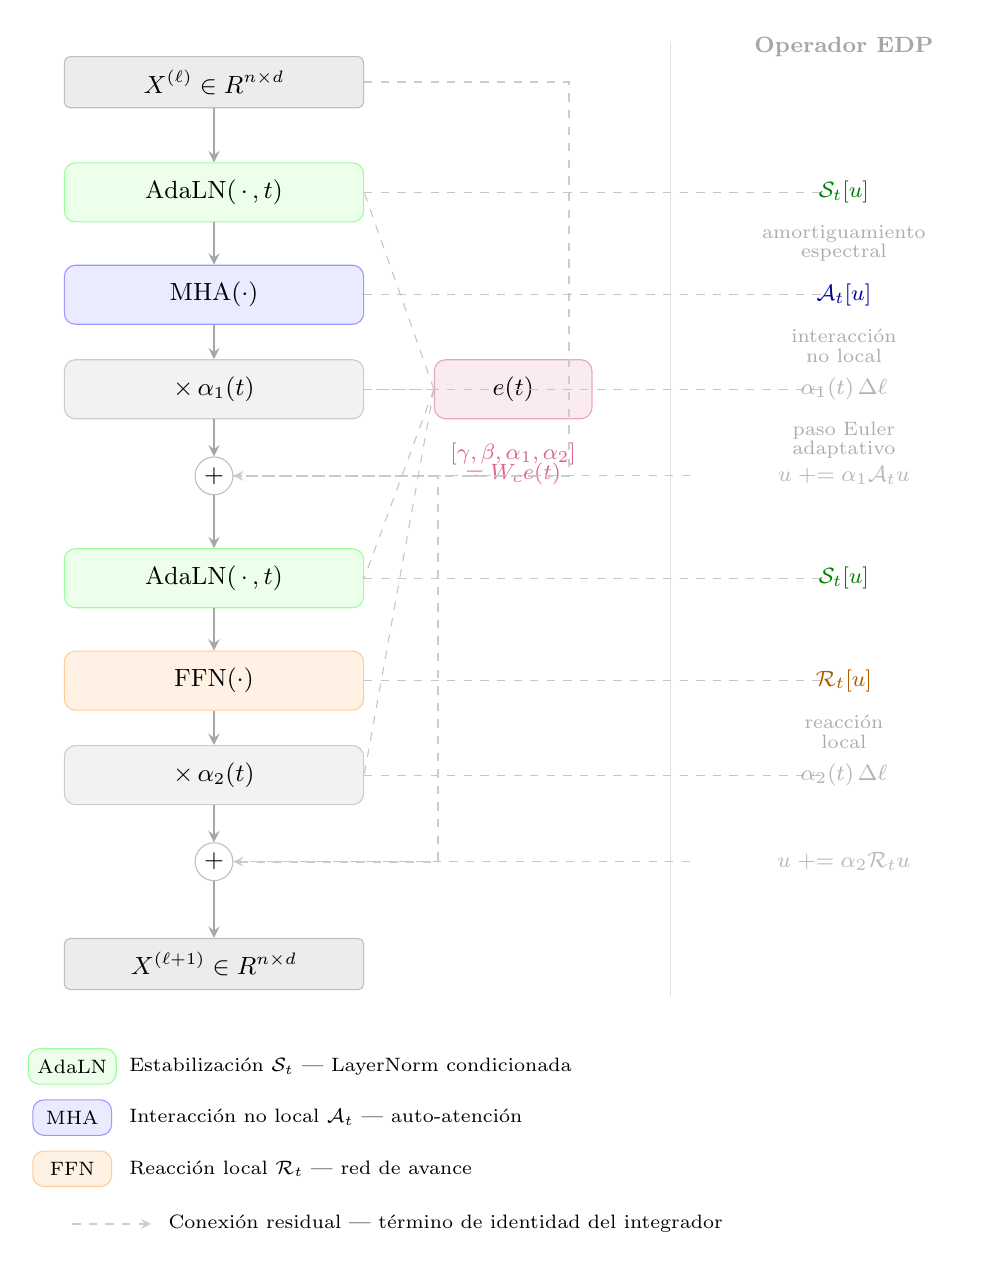
\begin{tikzpicture}[
  % ── estilos de nodos ──────────────────────────────────────
  block/.style={
    rectangle, rounded corners=4pt,
    minimum width=3.8cm, minimum height=0.75cm,
    text centered, font=\small,
    draw=gray!60, line width=0.4pt
  },
  blockA/.style={block,
    fill=blue!8,  draw=blue!40},   % atención
  blockR/.style={block,
    fill=orange!10, draw=orange!40}, % FFN / reacción
  blockS/.style={block,
    fill=green!8, draw=green!40},  % AdaLN / estabilización
  blockG/.style={block,
    fill=gray!10, draw=gray!40},   % gate / escalar
  io/.style={
    rectangle, rounded corners=2pt,
    minimum width=3.8cm, minimum height=0.65cm,
    text centered, font=\small\itshape,
    fill=gray!15, draw=gray!50, line width=0.4pt
  },
  % ── anotaciones EDP ───────────────────────────────────────
  edpbox/.style={
    rectangle, rounded corners=3pt,
    minimum width=3.4cm, minimum height=0.65cm,
    text centered, font=\footnotesize,
    draw=none, fill=none
  },
  % ── flechas ───────────────────────────────────────────────
  arr/.style={-stealth, gray!70, line width=0.8pt},
  arrres/.style={-stealth, gray!40, line width=0.6pt,
                 dashed},          % conexión residual
  leader/.style={gray!45, line width=0.4pt, dashed}
]

% ════════════════════════════════════════════════════════════
%  COLUMNA IZQUIERDA — flujo arquitectónico
% ════════════════════════════════════════════════════════════

\def\cx{0}      % centro de la columna de bloques
\def\cxr{2.4}   % punto de salida de la conexión residual

% -- Input ------------------------------------------------
\node[io] (in) at (\cx, 0)
  {$\bm{X}^{(\ell)} \in \mathbb{R}^{n \times d}$};

% -- AdaLN 1 (pre-norm, atención) -------------------------
\node[blockS] (ln1) at (\cx, -1.4)
  {$\mathrm{AdaLN}(\,\cdot\,,t)$};

% -- MHA --------------------------------------------------
\node[blockA] (mha) at (\cx, -2.7)
  {$\mathrm{MHA}(\cdot)$};

% -- Gate alpha_1 -----------------------------------------
\node[blockG] (g1) at (\cx, -3.9)
  {$\times\,\alpha_1(t)$};

% -- Suma residual 1 (nodo explícito) ---------------------
\node[circle, draw=gray!50, fill=white,
      inner sep=1.5pt, font=\small] (sum1) at (\cx, -5.0)
  {$+$};

% -- AdaLN 2 (pre-norm, FFN) ------------------------------
\node[blockS] (ln2) at (\cx, -6.3)
  {$\mathrm{AdaLN}(\,\cdot\,,t)$};

% -- FFN --------------------------------------------------
\node[blockR] (ffn) at (\cx, -7.6)
  {$\mathrm{FFN}(\cdot)$};

% -- Gate alpha_2 -----------------------------------------
\node[blockG] (g2) at (\cx, -8.8)
  {$\times\,\alpha_2(t)$};

% -- Suma residual 2 --------------------------------------
\node[circle, draw=gray!50, fill=white,
      inner sep=1.5pt, font=\small] (sum2) at (\cx, -9.9)
  {$+$};

% -- Output -----------------------------------------------
\node[io] (out) at (\cx, -11.2)
  {$\bm{X}^{(\ell+1)} \in \mathbb{R}^{n \times d}$};

% -- Embedding de tiempo (lateral) ------------------------
\node[block, fill=purple!8, draw=purple!35,
      minimum width=2.0cm, font=\small]
  (emb) at (3.8, -3.9)
  {$\bm{e}(t)$};

\node[font=\footnotesize, text=purple!60, align=center]
  at (3.8, -4.85)
  {$[\gamma,\beta,\alpha_1,\alpha_2]$\\[-2pt]$=\bm{W}_c\bm{e}(t)$};

% ── flechas principales ───────────────────────────────────
\draw[arr] (in)   -- (ln1);
\draw[arr] (ln1)  -- (mha);
\draw[arr] (mha)  -- (g1);
\draw[arr] (g1)   -- (sum1);
\draw[arr] (sum1) -- (ln2);
\draw[arr] (ln2)  -- (ffn);
\draw[arr] (ffn)  -- (g2);
\draw[arr] (g2)   -- (sum2);
\draw[arr] (sum2) -- (out);

% ── conexiones residuales (bypass) ────────────────────────
% residual 1: in -> sum1
\draw[arrres]
  (in.east) -- ++({\cxr - \cx + 0.2}, 0)
  -- ++(0, {-5.0 + 0.0})
  -- (sum1.east);

% residual 2: sum1 -> sum2
\draw[arrres]
  (sum1.east) -- ++({\cxr - \cx + 0.2}, 0)
  -- ++(0, {-4.9})
  -- (sum2.east);

% ── embedding conectado a AdaLN y gates ──────────────────
\draw[leader] (emb.west) -- (ln1.east);
\draw[leader] (emb.west) -- (ln2.east);
\draw[leader] (emb.west) -- (g1.east);
\draw[leader] (emb.west) -- (g2.east);

% ════════════════════════════════════════════════════════════
%  COLUMNA DERECHA — anotaciones EDP
% ════════════════════════════════════════════════════════════

\def\ex{8.0}   % x de las etiquetas EDP

% separador vertical
\draw[gray!25, line width=0.5pt] (5.8, 0.5) -- (5.8, -11.6);

\node[font=\footnotesize\bfseries, gray!70]
  at (\ex, 0.45) {Operador EDP};

% -- AdaLN <-> S ------------------------------------------
\draw[leader] (ln1.east) -- ++({(\ex - \cx - 1.9 - 0.2)}, 0);
\node[edpbox, text=green!50!black] at (\ex, -1.4)
  {$\mathcal{S}_t[\bm{u}]$};
\node[font=\scriptsize, text=gray!65, align=center]
  at (\ex, -2.05)
  {amortiguamiento\\[-1pt]espectral};

% -- MHA <-> A --------------------------------------------
\draw[leader] (mha.east) -- ++({(\ex - \cx - 1.9 - 0.2)}, 0);
\node[edpbox, text=blue!60!black] at (\ex, -2.7)
  {$\mathcal{A}_t[\bm{u}]$};
\node[font=\scriptsize, text=gray!65, align=center]
  at (\ex, -3.35)
  {interacción\\[-1pt]no local};

% -- Gate <-> coef. Euler ---------------------------------
\draw[leader] (g1.east) -- ++({(\ex - \cx - 1.9 - 0.2)}, 0);
\node[edpbox, text=gray!60] at (\ex, -3.9)
  {$\alpha_1(t)\,\Delta\ell$};
\node[font=\scriptsize, text=gray!65, align=center]
  at (\ex, -4.55)
  {paso Euler\\[-1pt]adaptativo};

% -- sum1 <-> discretización Euler ------------------------
\draw[leader] (sum1.east) -- ++({(\ex - \cx - 1.9 - 0.2)}, 0);
\node[edpbox, text=gray!55] at (\ex, -5.0)
  {$\bm{u} \mathrel{+}= \alpha_1\mathcal{A}_t\bm{u}$};

% -- AdaLN 2 <-> S ----------------------------------------
\draw[leader] (ln2.east) -- ++({(\ex - \cx - 1.9 - 0.2)}, 0);
\node[edpbox, text=green!50!black] at (\ex, -6.3)
  {$\mathcal{S}_t[\bm{u}]$};

% -- FFN <-> R --------------------------------------------
\draw[leader] (ffn.east) -- ++({(\ex - \cx - 1.9 - 0.2)}, 0);
\node[edpbox, text=orange!70!black] at (\ex, -7.6)
  {$\mathcal{R}_t[\bm{u}]$};
\node[font=\scriptsize, text=gray!65, align=center]
  at (\ex, -8.25)
  {reacción\\[-1pt]local};

% -- Gate 2 -----------------------------------------------
\draw[leader] (g2.east) -- ++({(\ex - \cx - 1.9 - 0.2)}, 0);
\node[edpbox, text=gray!60] at (\ex, -8.8)
  {$\alpha_2(t)\,\Delta\ell$};

% -- sum2 -------------------------------------------------
\draw[leader] (sum2.east) -- ++({(\ex - \cx - 1.9 - 0.2)}, 0);
\node[edpbox, text=gray!55] at (\ex, -9.9)
  {$\bm{u} \mathrel{+}= \alpha_2\mathcal{R}_t\bm{u}$};

% ════════════════════════════════════════════════════════════
%  LEYENDA
% ════════════════════════════════════════════════════════════

\begin{scope}[shift={(-1.8, -12.5)}]
  \node[blockS, minimum width=1.0cm, minimum height=0.45cm,
        font=\scriptsize] at (0,0)     {AdaLN};
  \node[font=\scriptsize, anchor=west] at (0.6, 0)
    {Estabilización $\mathcal{S}_t$ — LayerNorm condicionada};

  \node[blockA, minimum width=1.0cm, minimum height=0.45cm,
        font=\scriptsize] at (0,-0.65) {MHA};
  \node[font=\scriptsize, anchor=west] at (0.6,-0.65)
    {Interacción no local $\mathcal{A}_t$ — auto-atención};

  \node[blockR, minimum width=1.0cm, minimum height=0.45cm,
        font=\scriptsize] at (0,-1.3) {FFN};
  \node[font=\scriptsize, anchor=west] at (0.6,-1.3)
    {Reacción local $\mathcal{R}_t$ — red de avance};

  \draw[arrres] (0,-2.0) -- (1.0,-2.0);
  \node[font=\scriptsize, anchor=west] at (1.1,-2.0)
    {Conexión residual — término de identidad del integrador};
\end{scope}

\end{tikzpicture}

\caption{Arquitectura del bloque DiT y su correspondencia con los
operadores de la EDP maestra~\eqref{eq:master_pde_t}.
\textbf{Izquierda:} flujo de datos a través del bloque.
El embedding de tiempo $\bm{e}(t)$ (morado) genera simultáneamente
los parámetros de AdaLN ($\gamma, \beta$) y los gates adaptativos
($\alpha_1, \alpha_2$) para todas las capas.
Las líneas discontinuas representan las conexiones residuales
que implementan el término de identidad del integrador de Euler.
\textbf{Derecha:} operador de la EDP maestra~\eqref{eq:master_pde_t}
al que corresponde cada componente. La evolución discreta capa a capa
$\bm{u}^{(\ell+1)} = \bm{u}^{(\ell)}
+ \alpha_1(t)\mathcal{A}_t[\bm{u}^{(\ell)}]
+ \alpha_2(t)\mathcal{R}_t[\bm{u}^{(\ell)}]$
es el método de Euler aplicado a la EDP continua
$\partial_\ell \bm{u} = \mathcal{A}_t[\bm{u}] + \mathcal{R}_t[\bm{u}]$.}
\label{fig:dit_bloque}
\end{figure}

%────────────────────────────────────────────────────────────────
\section{Redes equivariantes de grupo: el caso SO(3)}
\label{sec:so3}
\dificultad{4}{3}
%────────────────────────────────────────────────────────────────

Esta sección desarrolla la forma canónica de las capas equivariantes
para el grupo de rotaciones $\mathrm{SO}(3)$. Requiere familiaridad
con la teoría de representaciones de grupos de Lie: armónicos
esféricos, matrices de Wigner y coeficientes de Clebsch-Gordan.
Un físico de partículas o de estructura nuclear reconocerá estos
objetos desde la mecánica cuántica del momento angular; un lector
sin ese background puede continuar al Capítulo~\ref{ch:cap10} sin
pérdida de continuidad. Las arquitecturas de difusión de los
Capítulos~\ref{ch:cap11}--\ref{ch:cap12} no dependen de esta sección.

\subsubsection*{Armónicos esféricos como base de las representaciones}

Los armónicos esféricos $Y_l^m: S^2 \to \mathbb{C}$ son las autofunciones del
operador de Laplace-Beltrami en la esfera $S^2$:
\[
  \nabla^2_{S^2} Y_l^m = -l(l+1)Y_l^m.
\]
Son ortogonales: $\int_{S^2} Y_l^m(\hat{\bm{r}})\overline{Y_{l'}^{m'}(\hat{\bm{r}})}\,
d\hat{\bm{r}} = \delta_{ll'}\delta_{mm'}$, y completos en $L^2(S^2)$.

Bajo una rotación $R \in \mathrm{SO}(3)$, los armónicos esféricos de grado $l$
transforman entre sí mediante la \textbf{matriz de Wigner} $\bm{D}^l(R)$:
\begin{equation}
  Y_l^m(R^{-1}\hat{\bm{r}}) = \sum_{m'=-l}^l D_{m'm}^l(R)\,Y_l^{m'}(\hat{\bm{r}}).
  \label{eq:wigner}
\end{equation}
Las matrices de Wigner $\bm{D}^l(R) \in \mathbb{C}^{(2l+1)\times(2l+1)}$
son exactamente las representaciones irreducibles de $\mathrm{SO}(3)$:
$\bm{D}^l: \mathrm{SO}(3) \to \mathrm{GL}(\mathbb{C}^{2l+1})$.

Para aplicaciones físicas reales se usan versiones reales $Y_l^m$ (combinaciones
lineales de las complejas), con matrices de Wigner reales correspondientes.

Los primeros armónicos (reales):
\begin{align*}
  l=0:&\quad Y_0^0 = \frac{1}{\sqrt{4\pi}} \quad (\text{invariante bajo rotaciones}) \\
  l=1:&\quad Y_1^{-1} \propto y/r,\; Y_1^0 \propto z/r,\; Y_1^1 \propto x/r
        \quad (\text{componentes de un vector}) \\
  l=2:&\quad \text{cinco componentes de un tensor simétrico sin traza.}
\end{align*}

\begin{fisicaconexion}{Armónicos esféricos en física atómica y electromagnetismo}
Los armónicos esféricos son ubicuos en física porque $\mathrm{SO}(3)$ es el
grupo de simetría de cualquier problema con simetría esférica. En
\textbf{mecánica cuántica}, los orbitales atómicos del hidrógeno son
$\psi_{nlm}(r,\theta,\phi) = R_{nl}(r)\,Y_l^m(\theta,\phi)$, donde $l$ es el
número cuántico de momento angular y $m$ el magnético. Los estados $s$, $p$,
$d$, $f$ corresponden a $l = 0, 1, 2, 3$: exactamente los primeros irreducibles
de $\mathrm{SO}(3)$. Las reglas de selección de las transiciones atómicas
($\Delta l = \pm 1$, $\Delta m = 0, \pm 1$) son las reglas de Clebsch-Gordan
del producto $V_l \otimes V_1$ (fotón de espín 1): solo los $l$ que aparecen
en la descomposición~\eqref{eq:cg_decomp} están permitidos.

En \textbf{electromagnetismo}, la expansión multipolar del potencial de una
distribución de carga a distancia $r \gg r'$ es:
\[
  \phi(\bm{r}) = \frac{1}{4\pi\epsilon_0}\sum_{l=0}^\infty \sum_{m=-l}^l
  \frac{4\pi}{2l+1}\,q_{lm}\,\frac{Y_l^m(\hat{\bm{r}})}{r^{l+1}},
\]
donde $q_{lm} = \int r'^l Y_l^{m*}(\hat{\bm{r}}')\rho(\bm{r}')d\bm{r}'$ son
los \textbf{momentos multipolares}: escalar ($l=0$), dipolo ($l=1$), cuadrupolo
($l=2$), etc. Los mismos $l$ que clasifican los irreducibles de $\mathrm{SO}(3)$
indexan los multipolos. En RMN, las matrices de Wigner $\bm{D}^l(R)$
aparecen al describir cómo los tensores de desplazamiento químico y acoplamiento
dipolar transforman bajo rotaciones de la muestra en experimentos de ángulo
mágico. La ecuación~\eqref{eq:wigner} no es solo una fórmula de redes neuronales:
es la ley de transformación de cualquier objeto tensorial de rango $l$ bajo
rotaciones.
\end{fisicaconexion}
\label{subsec:cg}

El producto tensorial de dos representaciones irreducibles de $\mathrm{SO}(3)$
de órdenes $l_1$ y $l_2$ se descompone en suma directa de irreducibles:
\begin{equation}
  V_{l_1} \otimes V_{l_2} \cong \bigoplus_{l=|l_1-l_2|}^{l_1+l_2} V_l.
  \label{eq:cg_decomp}
\end{equation}
Esta descomposición es la \textbf{regla de selección de Clebsch-Gordan}.
Los vectores de la base del irreducible $V_l$ en el producto $V_{l_1}\otimes V_{l_2}$
son:
\begin{equation}
  |l, m\rangle = \sum_{m_1=-l_1}^{l_1} \sum_{m_2=-l_2}^{l_2}
  C_{m_1 m_2 m}^{l_1 l_2 l}\,|l_1, m_1\rangle \otimes |l_2, m_2\rangle,
  \label{eq:cg_vector}
\end{equation}
donde $C_{m_1 m_2 m}^{l_1 l_2 l}$ son los \textbf{coeficientes de Clebsch-Gordan}.
Son cero a menos que $m = m_1+m_2$ y $|l_1-l_2| \leq l \leq l_1+l_2$.

En notación de operador, la proyección del producto tensorial sobre el irreducible
$V_l$ define el \textbf{producto tensorial de Clebsch-Gordan}:
\[
  (\bm{f}^{l_1} \otimes_{CG}^l \bm{g}^{l_2})_m
  = \sum_{m_1, m_2} C_{m_1 m_2 m}^{l_1 l_2 l}\,
  f_{m_1}^{l_1}\,g_{m_2}^{l_2}.
\]

\subsection{La capa equivariante bajo SO(3): derivación completa}
\label{subsec:so3_layer}

Una capa equivariante bajo $\mathrm{SO}(3)$ mapea
$\bm{f} = \bigoplus_{l_{\mathrm{in}}} \bm{f}^{l_{\mathrm{in}}}$ a
$\bm{h} = \bigoplus_{l_{\mathrm{out}}} \bm{h}^{l_{\mathrm{out}}}$,
donde $\bm{f}^{l_{\mathrm{in}}} \in \mathbb{R}^{(2l_{\mathrm{in}}+1)\times C_{l_{\mathrm{in}}}}$
son las características del tipo $l_{\mathrm{in}}$ (con $C_{l_{\mathrm{in}}}$
canales) y análogamente para la salida.

\begin{teorema}{Forma canónica de la capa equivariante bajo SO(3)}
\label{thm:so3_layer}
La capa lineal más general que es equivariante bajo $\mathrm{SO}(3)$ tiene la
forma:
\begin{equation}
  h_{m_{\mathrm{out}}, c_{\mathrm{out}}}^{l_{\mathrm{out}}}
  = \sum_{l_{\mathrm{in}}, l_f} \sum_{m_{\mathrm{in}}, m_f}
  \sum_{c_{\mathrm{in}}}
  C_{m_{\mathrm{in}} m_f m_{\mathrm{out}}}^{l_{\mathrm{in}} l_f l_{\mathrm{out}}}
  \cdot w_{c_{\mathrm{in}} c_{\mathrm{out}}}^{l_{\mathrm{in}} l_f l_{\mathrm{out}}}
  \cdot f_{m_{\mathrm{in}}, c_{\mathrm{in}}}^{l_{\mathrm{in}}}
  \cdot Y_{l_f}^{m_f}(\hat{\bm{r}}),
  \label{eq:so3_layer}
\end{equation}
donde $\hat{\bm{r}}$ es la dirección de una arista (en grafos moleculares),
$Y_{l_f}^{m_f}$ son los armónicos esféricos del edge, y $w_{c_{\mathrm{in}}
c_{\mathrm{out}}}^{l_{\mathrm{in}} l_f l_{\mathrm{out}}} \in \mathbb{R}$ son
los únicos parámetros libres aprendibles.
\end{teorema}

\begin{proof}
Por el Lema de Schur, $\bm{W}$ es equivariante si y solo si, en la
descomposición en irreducibles, solo conecta irreducibles del mismo tipo.
La representación de entrada en el nodo es $\bigoplus_{l_{\mathrm{in}}}
\bm{D}^{l_{\mathrm{in}}}$. Los armónicos esféricos de la arista transforman
como $\bigoplus_{l_f} \bm{D}^{l_f}$. El producto tensorial de la
característica de entrada y el armónico de la arista es:
\[
  V_{l_{\mathrm{in}}} \otimes V_{l_f}
  \cong \bigoplus_{l=|l_{\mathrm{in}}-l_f|}^{l_{\mathrm{in}}+l_f} V_l.
\]
Para conectar este producto con la salida $V_{l_{\mathrm{out}}}$, por el
Lema de Schur solo es posible si $l_{\mathrm{out}}$ aparece en la
descomposición, es decir $|l_{\mathrm{in}}-l_f| \leq l_{\mathrm{out}}
\leq l_{\mathrm{in}}+l_f$ (regla de selección de Clebsch-Gordan).
Dentro de cada bloque permitido, el Lema de Schur establece que el único
mapa lineal equivariante es un múltiplo escalar de la identidad en ese bloque:
ese escalar es exactamente $w_{c_{\mathrm{in}} c_{\mathrm{out}}}^{l_{\mathrm{in}}
l_f l_{\mathrm{out}}}$, con un grado de libertad por cada tripleta
$(l_{\mathrm{in}}, l_f, l_{\mathrm{out}})$ y par de canales $(c_{\mathrm{in}},
c_{\mathrm{out}})$ que satisfaga la regla de selección. El mapa explícito es
el producto de Clebsch-Gordan de~\eqref{eq:so3_layer}. $\square$
\end{proof}

\begin{observacion}{Conteo de parámetros equivariantes}
Para tipos de orden máximo $l_{\max}$, el número de tipos de irreducibles es
$l_{\max}+1$ y el número de tripletas permitidas $(l_{\mathrm{in}}, l_f,
l_{\mathrm{out}})$ es $O(l_{\max}^3)$. Los parámetros aprendibles son escalares:
el costo de la capa es $O(l_{\max}^3 C^2)$ parámetros (con $C$ canales por
tipo), significativamente menor que el costo de una capa densa no equivariante
de la misma dimensión, que sería $O((l_{\max}C)^2 (2l_{\max}+1)^2)$.
\end{observacion}

\subsection{Ejemplos de arquitecturas SO(3)-equivariantes}
\label{subsec:so3_arqs}

La estructura de la ecuación~\eqref{eq:so3_layer} aparece en múltiples
arquitecturas para datos 3D:

\medskip
\noindent\textbf{e3nn} (Geiger y Smidt, 2022): implementación modular de capas
equivariantes para cualquier grupo $O(3)$. Los tipos son \textit{scalars}
($l=0$), \textit{vectors} ($l=1$), \textit{tensors} ($l=2$, etc.).

\medskip
\noindent\textbf{NequIP/MACE} (Batzner et al., 2022; Batatia et al., 2022):
para potenciales interatómicos de aprendizaje automático. Las características
de los nodos son tensores esféricos de los átomos; las interacciones entre
pares de átomos se convoluciona con los armónicos esféricos de la dirección
interatómica. El resultado respeta exactamente las simetrías de traslación,
rotación y reflexión de la mecánica molecular.

\subsection{Construcción sistemática para grupos generales}
\label{subsec:grupo_general}

El procedimiento general para construir una capa equivariante bajo un grupo
compacto $G$ dado es:
\begin{enumerate}
  \item Calcular la tabla de caracteres de $G$: las trazas
        $\chi^\alpha(g) = \mathrm{tr}(\rho^\alpha(g))$ de cada clase de
        conjugación para cada irreducible $\rho^\alpha$.
  \item Descomponer las representaciones de entrada y salida en irreducibles
        usando las relaciones de ortogonalidad:
        $m_\alpha = \frac{1}{|G|}\sum_g \chi^\alpha(g^{-1})\chi_{\mathrm{in}}(g)$.
  \item Por el Lema de Schur, los únicos pesos libres son escalares que
        multiplican el mapa identidad en cada bloque de irreducibles equivalentes.
\end{enumerate}
Este procedimiento es completamente algorítmico y se implementa para cualquier
grupo finito o de Lie compacto.

%───────────────────────────────────────────────────────────────────────────────
\section{Conexiones residuales y Neural ODEs}
\label{sec:resnet_node}
\dificultad{3}{3}
%───────────────────────────────────────────────────────────────────────────────

\subsection{El problema del gradiente en redes profundas}
\label{subsec:grad_profundo}

Para un MLP de $L$ capas, el error de la capa $l$ es:
\[
  \bm{\delta}^{(l)}
  = \Biggl(\prod_{k=l+1}^L \bm{W}^{(k)\top}
    \mathrm{diag}(\sigma'^{(k)}(\bm{z}^{(k)}))\Biggr)\bm{\delta}^{(L)}.
\]
Si las normas espectrales de los jacobianos son en promedio $< 1$, el gradiente
se desvanece exponencialmente en $L-l$. Si son $> 1$, explota. Para $L = 100$
capas, incluso una norma media de $0.99$ da $0.99^{100} \approx 0.37$:
el gradiente llega a la primera capa con $37\%$ de su magnitud original,
lo que es manejable; pero una norma de $0.9$ da $0.9^{100} \approx 3\times 10^{-5}$:
el gradiente prácticamente desaparece.

\subsection{Las conexiones residuales como integrador de Euler}
\label{subsec:residual}

\begin{definicion}{Bloque residual}
\label{def:residual}
Un \textbf{bloque residual} (\textit{residual block}) es:
\[
  \bm{a}^{(l+1)} = \bm{a}^{(l)} + F(\bm{a}^{(l)};\bm{\theta}^{(l)}),
\]
donde $F$ es típicamente una secuencia de dos capas con normalización y
activación, y $\bm{a}^{(l)}$ y $F$ tienen la misma dimensión.
\end{definicion}

El backward pass de la conexión residual:
\[
  \bm{\delta}^{(l)} = \frac{\partial\mathcal{L}}{\partial\bm{a}^{(l)}}
  = \frac{\partial\mathcal{L}}{\partial\bm{a}^{(l+1)}}
  \cdot\left(\bm{I} + \frac{\partial F}{\partial\bm{a}^{(l)}}\right)
  = \bm{\delta}^{(l+1)}\left(\bm{I} + \bm{J}_F^{(l)}\right).
\]
El término identidad garantiza que el gradiente $\bm{\delta}^{(l+1)}$ llega
intacto a la capa $l$, independientemente de la magnitud de $\bm{J}_F^{(l)}$.
Para redes con $L = 100$--$1000$ bloques residuales, este mecanismo hace el
entrenamiento estable.

La interpretación como integrador: la ecuación
$\bm{a}^{(l+1)} = \bm{a}^{(l)} + F(\bm{a}^{(l)})$ es el método de Euler
con paso $h = 1$ para la ODE:
\[
  \frac{d\bm{a}}{dt} = F(\bm{a}(t);\bm{\theta}),
  \qquad \bm{a}(0) = \bm{a}^{(0)},
\]
con $\bm{a}^{(l)} = \bm{a}(l)$. La profundidad $L$ es el número de pasos
de Euler; la activación de la última capa es $\bm{a}(L)$, la solución
aproximada de la ODE.

\subsection{Neural ODEs: profundidad continua y el método adjunto completo}
\label{subsec:neural_ode}

La \textbf{Neural ODE} (Chen et al., 2018) toma este límite en serio: en lugar
de discretizar con $L$ pasos de Euler, usa un integrador numérico de alta
precisión para resolver la ODE exacta:
\begin{equation}
  \frac{d\bm{a}(t)}{dt} = F(\bm{a}(t), t;\bm{\theta}),
  \qquad \bm{a}(t_0) = \bm{a}^{(0)},
  \label{eq:neural_ode}
\end{equation}
y la predicción es $\hat{\bm{y}} = g(\bm{a}(t_1))$ donde $g$ es una capa de
salida. El forward pass es la integración numérica de~\eqref{eq:neural_ode}
de $t_0$ a $t_1$.

El problema del backward pass es calcular $\nabla_{\bm{\theta}}\mathcal{L}$
donde $\mathcal{L} = \ell(\hat{\bm{y}}, \bm{y}) = \ell(g(\bm{a}(t_1)),\bm{y})$.
La solución naïve (backpropagation a través de los pasos del integrador) requiere
almacenar todas las activaciones intermedias del integrador: para un integrador
de orden 4 con $N_{\text{steps}}$ pasos, esto es $O(N_{\text{steps}})$ en memoria.
La Neural ODE resuelve esto con el \textbf{método adjunto}, reduciendo el costo
de memoria a $O(1)$.

\subsubsection*{Derivación completa del método adjunto para Neural ODEs}

Se considera el problema general de minimizar $\mathcal{L} = \int_{t_0}^{t_1}
r(\bm{a}(t),\bm{\theta},t)\,dt + \ell(\bm{a}(t_1),\bm{y})$ sujeto a~\eqref{eq:neural_ode}.
Para la Neural ODE estándar $r = 0$.

\medskip
\noindent\textbf{Paso 1: el estado adjunto.}
Se define el \textbf{estado adjunto} (o co-estado):
\begin{equation}
  \bm{\lambda}(t) = \frac{d\mathcal{L}}{d\bm{a}(t)} \in \mathbb{R}^d.
  \label{eq:adjunto_def}
\end{equation}
La condición terminal es $\bm{\lambda}(t_1) = \frac{d\ell}{d\bm{a}(t_1)}
= \nabla_{\bm{a}(t_1)}\ell$.

\medskip
\noindent\textbf{Paso 2: la ecuación adjunta.}
Se calcula $d\bm{\lambda}/dt$ usando la fórmula de Itô para el funcional
continuo (o equivalentemente, diferenciando la identidad de sensibilidad).
Para un incremento $\delta t$, la variación $\delta\bm{a}(t)$ se propaga
según la ecuación variacional:
\[
  \frac{d}{dt}\delta\bm{a}(t)
  = \frac{\partial F(\bm{a}(t),t;\bm{\theta})}{\partial\bm{a}}\delta\bm{a}(t)
  = \bm{J}_F(t)\,\delta\bm{a}(t).
\]
La variación de la pérdida es:
\[
  \delta\mathcal{L} = \bm{\lambda}(t_1)^\top\delta\bm{a}(t_1)
  = \bm{\lambda}(t_1)^\top
  \underbrace{\left[\bm{I} + \int_t^{t_1}\bm{J}_F(s)\,ds + O(\Delta t^2)\right]}
  _{\text{propagador linealizado}}
  \delta\bm{a}(t).
\]
Diferenciando respecto a $t$:
\[
  \frac{d\bm{\lambda}(t)^\top}{dt}
  = -\bm{\lambda}(t)^\top\bm{J}_F(t),
\]
es decir:
\begin{equation}
  \frac{d\bm{\lambda}}{dt}
  = -\bm{J}_F(t)^\top\bm{\lambda}(t)
  = -\left(\frac{\partial F(\bm{a}(t),t;\bm{\theta})}{\partial\bm{a}}\right)^\top
  \bm{\lambda}(t).
  \label{eq:adj_ode}
\end{equation}
Esta es la \textbf{ecuación adjunta}: una ODE lineal no autónoma para
$\bm{\lambda}(t)$ que se integra \textbf{hacia atrás} desde $t_1$ hasta $t_0$.

\medskip
\noindent\textbf{Paso 3: el gradiente respecto a los parámetros.}
La variación de $\mathcal{L}$ respecto a un cambio $\delta\bm{\theta}$ en los
parámetros es, usando la fórmula de sensibilidad paramétrica:
\begin{equation}
  \frac{d\mathcal{L}}{d\bm{\theta}}
  = \int_{t_0}^{t_1}
  \bm{\lambda}(t)^\top
  \frac{\partial F(\bm{a}(t),t;\bm{\theta})}{\partial\bm{\theta}}\,dt.
  \label{eq:grad_theta}
\end{equation}

\medskip
\noindent\textbf{Paso 4: el algoritmo adjunto completo.}
El Algoritmo~\ref{alg:adj_ode} resume el procedimiento.

\begin{algorithm}[H]
\caption{Método adjunto para Neural ODEs}
\label{alg:adj_ode}
\KwIn{Red $F(\cdot,\cdot;\bm{\theta})$, pérdida $\ell$, entrada $\bm{a}^{(0)}$,
      intervalo $[t_0,t_1]$}
\KwOut{$\mathcal{L}$, $\nabla_{\bm{a}^{(0)}}\mathcal{L}$,
       $\nabla_{\bm{\theta}}\mathcal{L}$}

\tcp{--- Forward pass: integrar la Neural ODE ---}
$\bm{a}(t_1) \leftarrow \mathrm{ODESolve}\!\left(F,\,\bm{a}(t_0),\,[t_0,t_1]\right)$\;
$\mathcal{L} \leftarrow \ell(\bm{a}(t_1),\bm{y})$\;

\tcp{--- Inicializar el estado adjunto ---}
$\bm{\lambda}(t_1) \leftarrow \nabla_{\bm{a}(t_1)}\ell$\;
$\bm{a}_{\bm{\theta}}(t_1) \leftarrow \bm{0}$ \tcp*{acumulador del gradiente}

\tcp{--- Backward pass: integrar la ecuación adjunta hacia atrás ---}
$\begin{pmatrix}\bm{a}(t_0)\\\bm{\lambda}(t_0)\\\nabla_{\bm{\theta}}\mathcal{L}\end{pmatrix}
\leftarrow
\mathrm{ODESolve}\!\left(
  \begin{pmatrix}
    F(\bm{a},t;\bm{\theta})\\
    -\bm{J}_F^\top\bm{\lambda}\\
    -\bm{\lambda}^\top\partial_{\bm{\theta}}F
  \end{pmatrix},\;
  \begin{pmatrix}\bm{a}(t_1)\\\bm{\lambda}(t_1)\\\bm{0}\end{pmatrix},\;
  [t_1,t_0]\right)$\;

\Return $\mathcal{L}$, $\bm{\lambda}(t_0)$,
        $\nabla_{\bm{\theta}}\mathcal{L}$\;
\end{algorithm}

\subsubsection*{Correspondencia con el principio de Pontryagin}

La conexión con el formalismo del Capítulo~\ref{ch:cap6} es exacta. Identificando:
\begin{center}
\begin{tabular}{ll}
\toprule
\textbf{Neural ODE} & \textbf{MLP (Cap.~\ref{ch:cap6})} \\
\midrule
Estado $\bm{a}(t)$ & Post-activación $\bm{a}^{(l)}$ \\
Control $\bm{\theta}$ & Parámetros $(\bm{W}^{(l)},\bm{b}^{(l)})$ \\
ODE $\dot{\bm{a}} = F(\bm{a},t;\bm{\theta})$ & Forward pass discreto \\
Co-estado $\bm{\lambda}(t)$ & Error $\bm{\delta}^{(l)} = -\bm{\lambda}^{(l)}$ \\
Ec.\ adjunta $\dot{\bm{\lambda}} = -\bm{J}_F^\top\bm{\lambda}$ & BP2 continua \\
Condición terminal $\bm{\lambda}(t_1) = \nabla\ell$ & BP1 \\
Gradiente $\int\bm{\lambda}^\top\partial_{\bm{\theta}}F\,dt$ & BP3 acumulado \\
\bottomrule
\end{tabular}
\end{center}

El MLP del Capítulo~\ref{ch:cap4} es una Neural ODE discretizada con el método de Euler.
El método adjunto del Capítulo~\ref{ch:cap6} es la discretización del Algoritmo~\ref{alg:adj_ode}.
El principio de Pontryagin es el caso continuo de backpropagation.

\subsubsection*{Ventajas y costo del método adjunto}

\medskip
\noindent\textbf{Memoria $O(1)$:} el backward pass no requiere almacenar las
activaciones intermedias del forward pass: las recomputa integrando la ODE
del estado hacia atrás en paralelo con la ecuación adjunta. El costo de memoria
es $O(d + p)$ (estado más parámetros), independiente del número de pasos del
integrador.

\medskip
\noindent\textbf{Costo computacional:} el backward pass requiere integrar
numéricamente el sistema aumentado de dimensión $2d + p$ en lugar de $d$.
El costo es $\sim 3\times$ el del forward pass, idéntico al de backpropagation
estándar.

\medskip
\noindent\textbf{Precisión adaptativa:} el integrador del backward pass puede
elegir el paso adaptativo para controlar el error numérico de la ecuación
adjunta. En backpropagation estándar, el error numérico se acumula fijo capa
a capa.

\begin{fisicaconexion}{Ecuaciones diferenciales en física y el método adjunto en control óptimo}
La Neural ODE~\eqref{eq:neural_ode} es formalmente idéntica a la ecuación de
movimiento de un sistema dinámico con estado $\bm{a}(t)$ y campo de fuerza
$F(\bm{a},t;\bm{\theta})$. Para un oscilador anarmónico $\ddot{x} = -\omega^2 x -
\epsilon x^3$, la ecuación de segundo orden se escribe como sistema de primer
orden $\dot{\bm{a}} = (a_2, -\omega^2 a_1 - \epsilon a_1^3)$: exactamente la
forma de~\eqref{eq:neural_ode}, con $F$ determinado por la física en lugar de
aprendido.

El método adjunto del Algoritmo~\ref{alg:adj_ode} es la forma continua del
\textbf{principio del mínimo de Pontryagin} en teoría de control óptimo. El
problema clásico de control de trayectoria de un cohete o satélite es:
minimizar el combustible consumido $\mathcal{L} = \int_0^T \|\bm{u}(t)\|^2\,dt$
sujeto a la dinámica $\dot{\bm{x}} = f(\bm{x},\bm{u})$ (ecuación del
movimiento), con condición final $\bm{x}(T) = \bm{x}_f$ (destino). El método
adjunto introduce el \textbf{co-estado} $\bm{p}(t)$ (el vector de multiplicadores
de Lagrange en el tiempo) que satisface exactamente la ecuación adjunta
$\dot{\bm{p}} = -(\partial f/\partial \bm{x})^\top\bm{p}$: la misma
ecuación~\eqref{eq:adj_ode}. El control óptimo es $\bm{u}^*(t) = -\bm{p}(t)/2$
(para este caso cuadrático), obtenido sin integrar la dinámica en sentido
inverso.

En \textbf{óptica geométrica}, la ecuación eikonal $|\nabla S| = n(\bm{r})$
(con $S$ el frente de onda y $n$ el índice de refracción) tiene la misma
estructura: los rayos de luz son trayectorias del sistema hamiltoniano
$\dot{\bm{q}} = \bm{p}/n$, $\dot{\bm{p}} = \nabla n$. El estado adjunto de un
problema de diseño de lentes (minimizar aberración sujeto a la propagación de
rayos) es exactamente el vector de sensibilidad del frente de onda respecto a
los parámetros de la lente —la misma cantidad que se calcula en el paso
backward del Algoritmo~\ref{alg:adj_ode}.
\end{fisicaconexion}

\medskip
\noindent\textbf{Gancho hacia el Capítulo~\ref{ch:cap12}:} una Neural ODE perturbada con
ruido browniano es una SDE:
\[
  d\bm{a}(t) = F(\bm{a}(t),t;\bm{\theta})\,dt + g(t)\,d\bm{W}_t.
\]
El proceso inverso de esta SDE es exactamente el reverse SDE de Anderson
(Capítulo~\ref{ch:cap11}) con el score $\nabla_{\bm{a}}\log p_t(\bm{a})$ jugando el rol
del co-estado $\bm{\lambda}$. Los modelos de difusión del Capítulo~\ref{ch:cap12} son
Neural ODEs estocásticas cuyo entrenamiento requiere estimar ese score.

%───────────────────────────────────────────────────────────────────────────────
\section{Resumen del Capítulo 9}
\label{sec:resumen9}
%───────────────────────────────────────────────────────────────────────────────

El hilo de este capítulo es uno: imponer la simetría correcta restringe el
espacio de hipótesis al subconjunto de funciones relevantes, reduciendo la
complejidad efectiva (Proposición~\ref{prop:vc_simetria}) sin sacrificar la
capacidad de aproximar las funciones que satisfacen esa simetría. El Lema de
Schur (Lema~\ref{lema:schur}) determina la estructura algebraica de cualquier
capa equivariante para cualquier grupo: las CNNs son el caso del grupo de
traslaciones, las GNNs son el caso del grupo de permutaciones, las redes
equivariantes de $\mathrm{SO}(3)$ son el caso del grupo de rotaciones en 3D.

Las GNNs con paso de mensajes son exactamente tan expresivas como el test WL-1
(Teorema~\ref{thm:gnn_wl}): no más, no menos. Esta cota es consecuencia de la
estructura del agregador simétrico y puede superarse con características
estructurales o test WL de orden superior.

Las Neural ODEs son el límite continuo de las redes residuales. Su backward
pass es el método adjunto de Pontryagin, el mismo que se desarrolló en el
Capítulo~\ref{ch:cap6} para el MLP discreto. La dualidad forward/backward es la dualidad
estado/co-estado de los sistemas Hamiltonianos: la backpropagation es mecánica
analítica sobre el grafo computacional.

El capítulo siguiente (Cap.~\ref{ch:cap10}) completará el cálculo de Itô riguroso que el
Capítulo~\ref{ch:cap5} introdujo en contexto. El Capítulo~\ref{ch:cap11} desarrollará la ecuación de
Fokker-Planck y el time reversal de SDEs: las herramientas que hacen que el
término de ruido de la Neural ODE estocástica sea invertible y que el score
function sea el campo de deriva del proceso reverso. El Capítulo~\ref{ch:cap12} usará
todo lo anterior para construir y entrenar modelos de difusión.

%───────────────────────────────────────────────────────────────────────────────
\label{sec:estrella9}
\begin{estrella}{Simetrías en reconstrucción de calorímetros y análisis de jets}

\textbf{Simetría del calorímetro y equivarianza de traslación.}
Un calorímetro de alta energía (ATLAS, CMS) tiene geometría cilíndrica:
las celdas se indexan por pseudorrapidez $\eta$ y ángulo azimutal $\phi$, con
coordenadas discretas $(\eta_i, \phi_i) \in \mathbb{Z}^2$ en la cuadrícula de
torres. La física de la lluvia electromagnética es (aproximadamente) invariante
bajo traslaciones en $(\eta, \phi)$: un electrón de $50\,$GeV produce el mismo
patrón de depósito independientemente de su posición en el calorímetro.

Esta es exactamente la condición del Teorema~\ref{thm:conv_equivar}: el
estimador de energía o posición del electrón debe ser equivariante bajo
traslación en $(\eta, \phi)$. Por tanto, la arquitectura óptima para procesar
depósitos de energía en el calorímetro como mapa $(\eta, \phi) \to E$ es una
CNN 2D sobre la cuadrícula de torres. Arquitecturas como \textbf{CaloFlow},
\textbf{CaloDiT} y los emuladores de GEANT4 del Capítulo~\ref{ch:cap12}
explotan esta simetría explícitamente. Los núcleos aprendidos de las primeras
capas reproducen los filtros de bordes y curvatura esperados de la función de
forma lateral de la lluvia.

\textbf{Simetría de permutación en análisis de jets.}
Un jet hadrónico es una colección de partículas $\{\bm{p}_1, \ldots, \bm{p}_n\}$
sin orden intrínseco: el etiquetado de las partículas por el detector es
arbitrario. Una red que clasifique jets (por ejemplo, para discriminar jets de
quarks $b$ vs.\ jets de gluones) debe ser $S_n$-invariante. El
Teorema~\ref{thm:deepsets} garantiza que la arquitectura óptima tiene forma
$f = \rho(\sum_i \phi(\bm{p}_i))$: exactamente el modelo DeepSets. Las
arquitecturas de jet tagging modernas (ParticleNet, ParT, PELICAN) implementan
variantes de MPNNs sobre el grafo de partículas del jet, donde los nodos son
las partículas y las aristas codifican relaciones angulares $\Delta R_{ij} =
\sqrt{(\Delta\eta_{ij})^2 + (\Delta\phi_{ij})^2}$. La expresividad de estos
modelos está acotada por el Teorema~\ref{thm:gnn_wl}: no pueden distinguir
configuraciones de jet que WL-1 no distingue, lo que tiene consecuencias
para la discriminación de jets con substructura compleja.

\textbf{Equivarianza SO(3) en reconstrucción de trazas y física nuclear.}
Para la reconstrucción de trazas de partículas cargadas en un detector con campo
magnético, la simetría natural es la invarianza bajo rotaciones del sistema de
coordenadas: la helicidad de una traza en el campo $\bm{B} = B\hat{z}$ es un
invariante del grupo $\mathrm{SO}(2)$ (rotaciones azimutales). Las arquitecturas
de la Sección~\ref{sec:so3} aplicadas a nubes de puntos 3D de trazas garantizan
que el score de clasificación o la reconstrucción del vértice primario no
dependan de la orientación del sistema de referencia del laboratorio.

En el contexto del IAN-R1, el campo de flujo neutrónico $\Phi(r, z)$ del reactor
tiene simetría cilíndrica $\mathrm{SO}(2) \times \mathbb{Z}_2$ (rotaciones
azimutales y reflexión axial). Un sustituto MLP que explote esta simetría
necesita la mitad de los datos de entrenamiento que uno denso sin sesgo
inductivo: en el régimen de datos escasos (pocas simulaciones de referencia
costosas), el inductive bias es directamente generalización con menos datos.
La Proposición~\ref{prop:vc_simetria} cuantifica la ganancia: la VC-dimensión
se reduce por un factor $|\mathrm{SO}(2)|$ (continuo, efectivamente por el
número de modos azimutales relevantes $\sim n_\phi$).
\end{estrella}

%───────────────────────────────────────────────────────────────────────────────
\section*{Ejercicios computacionales}
\addcontentsline{toc}{section}{Ejercicios computacionales}
%───────────────────────────────────────────────────────────────────────────────

\begin{ejerciciocomp}{Verificación de equivarianza y conteo de parámetros}
\textbf{Objetivo:} verificar numéricamente el Teorema~\ref{thm:conv_equivar}
y la Proposición~\ref{prop:vc_simetria} para la CNN y para la capa equivariante
bajo $C_4$.

\medskip\noindent\textbf{Algoritmo:}
\begin{enumerate}
  \item Crear una imagen $8 \times 8$ aleatoria $\bm{X}$ y un núcleo
        $3 \times 3$ aleatorio $\bm{K}$. Calcular $\bm{Y} = \bm{X} * \bm{K}$
        y $(T_{\bm{v}}\bm{X}) * \bm{K}$. Verificar que el resultado coincide
        con $T_{\bm{v}}(\bm{X} * \bm{K})$ para desplazamientos aleatorios
        $\bm{v}$. Reportar el error máximo.
  \item Implementar una capa densa $64 \to 64$ y una capa $C_4$-equivariante
        para imágenes $8 \times 8$ (4 orientaciones, pesos compartidos por
        órbita). Contar los parámetros libres de cada una. ¿Coincide con la
        predicción de la Proposición~\ref{prop:vc_simetria}?
  \item Entrenar ambas en un dataset de dígitos rotados ($N=500$ muestras,
        con rotaciones aleatorias de $0°$, $90°$, $180°$, $270°$). Registrar
        el error de validación en función de $N$. ¿Para qué $N$ la capa
        equivariante supera a la densa?
\end{enumerate}

\medskip\noindent\textbf{Verificación:} la equivarianza debe tener error
$< 10^{-6}$ (error numérico de punto flotante). La relación de parámetros debe
ser $\approx 1/4$, consistente con $|C_4| = 4$.
\end{ejerciciocomp}

\begin{ejerciciocomp}{GIN vs.\ media-agregador: expresividad práctica}
\textbf{Objetivo:} verificar experimentalmente el Teorema~\ref{thm:gnn_wl}
y mostrar que el agregador media es estrictamente menos expresivo que la suma.

\medskip\noindent\textbf{Algoritmo:}
\begin{enumerate}
  \item Construir tres grafos: $G_1$ = triángulo ($K_3$), $G_2$ = camino
        de 3 nodos ($P_3$), $G_3$ = par de aristas ($2K_2$). Verificar
        manualmente qué pares distingue WL-1.
  \item Implementar una MPNN con agregador \texttt{sum} y otra con agregador
        \texttt{mean}, ambas con $\phi_m = \phi_h = \mathrm{MLP}(64, 64)$ y
        $T = 3$ capas. Inicializar con los mismos pesos.
  \item Para cada par de grafos que WL-1 distingue, verificar que la GIN
        (\texttt{sum}) produce embeddings distintos y la GCN (\texttt{mean})
        puede no hacerlo. Construir un contraejemplo concreto donde la media
        colapsa dos grafos distintos.
  \item Añadir la característica estructural ``número de triángulos por nodo''
        como input. ¿Puede ahora la GCN distinguir todos los pares?
\end{enumerate}
\end{ejerciciocomp}

\begin{ejerciciocomp}{El transformer como integrador de Euler: verificación numérica}
\textbf{Objetivo:} verificar que las conexiones residuales implementan
el método de Euler para una ODE, y que LayerNorm actúa como
estabilizador espectral.

\medskip\noindent\textbf{Algoritmo:}
\begin{enumerate}
  \item Implementar un transformer minimalista de 4 capas sobre
        secuencias de longitud $n=16$ con $d=32$. Registrar la norma
        de las activaciones $\|\bm{u}^{(\ell)}\|$ en cada capa durante
        el forward pass.
  \item Repetir sin conexiones residuales (reemplazar
        $\bm{u}^{(\ell+1)} = \bm{u}^{(\ell)} + F(\bm{u}^{(\ell)})$
        por $\bm{u}^{(\ell+1)} = F(\bm{u}^{(\ell)})$). Comparar el
        crecimiento de $\|\bm{u}^{(\ell)}\|$ con y sin residuales.
        ¿La norma crece, decae o permanece estable?
  \item Repetir sin LayerNorm pero con residuales. Inicializar los
        pesos con varianza $\sigma^2 = 1/d$ en lugar de la
        inicialización estándar de Xavier. Observar si el entrenamiento
        diverge.
  \item Implementar AdaLN según la ecuación~\eqref{eq:adialn} con
        un embedding de tiempo $\bm{e}(t) = [\sin(\omega_k t)]_{k=1}^{d_t}$
        (embedding sinusoidal). Verificar que el gradiente
        $\partial\mathcal{L}/\partial t$ es no nulo para la mayoría de
        las capas simultáneamente.
\end{enumerate}

\medskip\noindent\textbf{Verificación:} con residuales y LayerNorm,
la norma debe mantenerse en $O(1)$. Sin LayerNorm, debe crecer al
menos como $1.1^\ell$ para $\ell = 4$ capas con pesos aleatorios de
varianza $1/d$.
\end{ejerciciocomp}

%───────────────────────────────────────────────────────────────────────────────
\begin{notasbib}
El principio de inductive bias estructural fue articulado en el contexto del
aprendizaje con simetrías por Cohen y Welling (2016)~\cite{cohen2016group}, que
introdujeron las G-CNNs como generalización de las CNNs a grupos discretos
arbitrarios. La formulación rigurosa vía el Lema de Schur y la teoría de
representaciones se desarrolló en Kondor y Trivedi (2018)~\cite{kondor2018clebsch}
y Weiler et al.\ (2019)~\cite{weiler2019general}. La reducción de
VC-dimensión bajo simetría (Proposición~\ref{prop:vc_simetria}) sigue a
la argumentación de Zaheer et al.\ (2017)~\cite{zaheer2017deep}.

La caracterización de las CNNs como única capa equivariante bajo traslación
(Teorema~\ref{thm:conv_equivar}) es clásica; su versión moderna aparece en
Bronstein et al.\ (2021)~\cite{bronstein2021geometric}. DeepSets
(Teorema~\ref{thm:deepsets}) fue introducido por Zaheer et al.\
(2017)~\cite{zaheer2017deep}. El marco unificado de message passing para GNNs
(Definición~\ref{def:mpnn}) es de Gilmer et al.\ (2017)~\cite{gilmer2017neural}.
La caracterización de la expresividad de las MPNNs via el test de
Weisfeiler-Leman (Teorema~\ref{thm:gnn_wl}) y la introducción de la GIN son de
Xu et al.\ (2019)~\cite{xu2019powerful}. Para una revisión completa del campo,
véase Bronstein et al.\ (2021).

La atención escalada y el transformer fueron introducidos por Vaswani et al.\
(2017)~\cite{vaswani2017attention}. La interpretación del transformer sin
codificación posicional como GNN completamente conectada aparece en Joshi
(2020) y Bronstein et al.\ (2021).

Las redes equivariantes bajo $\mathrm{SO}(3)$ usando armónicos esféricos y
coeficientes de Clebsch-Gordan fueron desarrolladas por Thomas et al.\
(2018)~\cite{thomas2018tensor}. La implementación modular \texttt{e3nn} es de
Geiger y Smidt (2022)~\cite{geiger2022e3nn}. Las arquitecturas NequIP y MACE
para potenciales interatómicos son de Batzner et al.\
(2022)~\cite{batzner2022nequip} y Batatia et al.\
(2022)~\cite{batatia2022mace}. La construcción sistemática para grupos generales
vía tablas de caracteres es estándar en teoría de representaciones; véase Serre
(1977)~\cite{serre1977linear}.

Las conexiones residuales y las ResNets fueron introducidas por He et al.\
(2016)~\cite{he2016deep}. La interpretación de las ResNets como integrador de
Euler y el límite Neural ODE son de Chen et al.\
(2018)~\cite{chen2018neural}, ya citado en el Capítulo~\ref{ch:cap6}. El
principio del mínimo de Pontryagin en control óptimo, cuya estructura se
corresponde con la ecuación adjunta~\eqref{eq:adj_ode}, es de Pontryagin et al.\
(1962)~\cite{pontryagin1962mathematical}; su conexión con el entrenamiento de
redes profundas fue analizada por Li y Hao (2018).
\end{notasbib}

%───────────────────────────────────────────────────────────────────────────────
\section*{Ejercicios resueltos}
\addcontentsline{toc}{section}{Ejercicios resueltos}
%───────────────────────────────────────────────────────────────────────────────

\begin{ejercicio}
\label{ej:conv_equivar}
\textbf{(Verificación de equivarianza de traslación).}

Sea $f: \mathbb{Z} \to \mathbb{R}$ una señal 1D y $k = (1, 0, -1)$ un núcleo
de diferencia finita. Verificar explícitamente que la convolución
$(f * k)[n] = f[n-1] - f[n+1]$ es equivariante bajo traslación:
$(T_v f) * k = T_v(f * k)$.

\medskip\noindent\textit{Solución.}
$(T_v f)[n] = f[n-v]$. Entonces:
\[
  ((T_v f)*k)[n]
  = (T_v f)[n-1]\cdot 1 + (T_v f)[n+1]\cdot(-1)
  = f[n-v-1] - f[n-v+1].
\]
Por otro lado:
\[
  (T_v(f*k))[n] = (f*k)[n-v] = f[n-v-1] - f[n-v+1].
\]
Coinciden: la convolución es equivariante bajo traslación. $\square$
\end{ejercicio}

\begin{ejercicio}
\label{ej:wl_falla}
\textbf{(Un par de grafos que WL-1 no distingue).}

Considerar el grafo $C_6$ (ciclo de 6 nodos) y el grafo $K_{3,3}$ (grafo
bipartito completo). Ambos son 2-regulares con 6 nodos y 6 aristas (tras
quitar algunas aristas de $K_{3,3}$ para igualarlo). Verificar que WL-1
asigna el mismo histograma de colores en cada iteración.

\medskip\noindent\textit{Solución.}
En $C_6$: todos los nodos tienen grado 2 y vecindarios isomorfos (dos vecinos
de grado 2). El color de cada nodo en la iteración $t$ es
$c^{(t)} = \mathrm{hash}(c^{(t-1)}, \{\!\{c^{(t-1)}, c^{(t-1)}\}\!\})$:
el mismo para todos, pues todos los nodos son equivalentes por simetría.

Para $K_{3,3}$ (bipartito completo): todos los nodos tienen grado 3. Tras
quitar 3 aristas para obtener un 2-regular bipartito, cada nodo tiene exactamente
dos vecinos del otro grupo. El color en cada iteración es también el mismo para
todos. Los histogramas de colores de ambos grafos coinciden en toda iteración:
WL-1 no los distingue, aunque $C_6$ contiene triángulos (ciclos de longitud 3)
y el 2-regular bipartito no (los ciclos más cortos en bipartitos son de
longitud 4). Una GNN-MPNN tampoco los distinguiría: necesitaría información
sobre la longitud de los ciclos (una característica estructural) o usar 3-WL.
$\square$
\end{ejercicio}

\begin{ejercicio}
\label{ej:adj_lineal}
\textbf{(Método adjunto para una ODE lineal).}

Sea $\dot{\bm{a}} = \bm{A}\bm{a}$ con $\bm{A} \in \mathbb{R}^{d\times d}$,
$\bm{a}(0) = \bm{a}_0$, y pérdida $\mathcal{L} = \frac{1}{2}\|\bm{a}(T)-
\bm{a}^*\|^2$. Calcular $\nabla_{\bm{a}_0}\mathcal{L}$ usando el método
adjunto y verificar que coincide con el resultado de backpropagation directo.

\medskip\noindent\textit{Solución.}
\textbf{Forward:} $\bm{a}(T) = e^{\bm{A}T}\bm{a}_0$.

\textbf{Estado adjunto inicial:}
$\bm{\lambda}(T) = \nabla_{\bm{a}(T)}\mathcal{L} = \bm{a}(T)-\bm{a}^*$.

\textbf{Ecuación adjunta:}
$\dot{\bm{\lambda}}(t) = -\bm{A}^\top\bm{\lambda}(t)$,
con solución $\bm{\lambda}(t) = e^{-\bm{A}^\top(t-T)}\bm{\lambda}(T)$.

\textbf{Gradiente:}
$\nabla_{\bm{a}_0}\mathcal{L} = \bm{\lambda}(0) = e^{\bm{A}^\top T}\bm{\lambda}(T)
= e^{\bm{A}^\top T}(e^{\bm{A}T}\bm{a}_0-\bm{a}^*)$.

\textbf{Verificación directa:}
$\mathcal{L} = \frac{1}{2}\|e^{\bm{A}T}\bm{a}_0-\bm{a}^*\|^2$,
$\nabla_{\bm{a}_0}\mathcal{L} = e^{\bm{A}^\top T}(e^{\bm{A}T}\bm{a}_0-\bm{a}^*)$.
Coinciden. $\square$
\end{ejercicio}

%───────────────────────────────────────────────────────────────────────────────
\section*{Ejercicios propuestos}
\addcontentsline{toc}{section}{Ejercicios propuestos}
%───────────────────────────────────────────────────────────────────────────────

\begin{ejercicio}
\textbf{(Equivarianza bajo rotaciones discretas $C_4$).}
Sea $G = C_4 = \{R_0, R_{90}, R_{180}, R_{270}\}$ el grupo de rotaciones de
$90°$ de imágenes cuadradas.
\begin{enumerate}[label=(\alph*)]
  \item Escribir las matrices de representación $\rho(R_k)$ para
        $k = 0, 90, 180, 270$ actuando sobre píxeles de una imagen $4\times 4$.
  \item Por el Lema de Schur, ¿cuál es la estructura de los pesos de una capa
        lineal $C_4$-equivariante?
  \item Implementar un MLP denso y una capa $C_4$-equivariante para clasificar
        imágenes de dígitos rotados. Comparar la exactitud de validación con
        el mismo número de parámetros.
  \item ¿Cuántos parámetros libres tiene la capa equivariante vs.\ la capa
        densa? ¿Es consistente con la Proposición~\ref{prop:vc_simetria}?
\end{enumerate}
\end{ejercicio}

\begin{ejercicio}
\textbf{(GIN vs.\ GCN en grafos simples).}
\begin{enumerate}[label=(\alph*)]
  \item Implementar la GCN (Graph Convolutional Network, Kipf y Welling, 2017)
        y la GIN (Graph Isomorphism Network, Xu et al., 2019) con $T=3$ capas.
  \item Construir el par de grafos del Ejercicio Resuelto~\ref{ej:wl_falla}.
        Verificar numéricamente que ambas GNNs producen el mismo embedding
        de grafo para los dos grafos.
  \item Añadir como característica de nodo el número de triángulos en los
        que participa cada nodo. ¿Pueden ahora las GNNs distinguir los grafos?
  \item ¿Cuántas capas se necesitan en la GIN para que la información de
        un nodo llegue a todos los nodos del grafo? ¿Es suficiente con
        $T = \mathrm{di\acute{a}metro}(\mathcal{G})$?
\end{enumerate}
\end{ejercicio}

\begin{ejercicio}
\textbf{(Coeficientes de Clebsch-Gordan para SO(3)).}
\begin{enumerate}[label=(\alph*)]
  \item Calcular los coeficientes $C_{m_1 m_2 m}^{1\,1\,l}$ para la
        descomposición $V_1 \otimes V_1 = V_0 \oplus V_1 \oplus V_2$
        usando las tablas estándar (o la fórmula de recurrencia de
        Condon-Shortley).
  \item Para dos vectores $\bm{f} \in \mathbb{R}^3$ (tipo $l=1$),
        calcular el producto de Clebsch-Gordan $\bm{f} \otimes_{CG}^0 \bm{g}$
        (escalar). ¿Es el producto escalar ordinario?
  \item Calcular $\bm{f} \otimes_{CG}^1 \bm{g}$ (vector). ¿Es el producto
        vectorial $\bm{f}\times\bm{g}$?
  \item Calcular $\bm{f} \otimes_{CG}^2 \bm{g}$ (tensor de rango 2 simétrico
        sin traza). Comparar con el tensor $f_i g_j + f_j g_i - \frac{2}{3}
        \delta_{ij}\bm{f}\cdot\bm{g}$.
\end{enumerate}
\end{ejercicio}

\begin{ejercicio}
\textbf{(Neural ODE como modelo generativo simple).}
\begin{enumerate}[label=(\alph*)]
  \item Implementar una Neural ODE con $F(\bm{a},t;\bm{\theta}) =
        \mathrm{MLP}([\bm{a}; t];\bm{\theta})$ (concatenar tiempo y estado).
  \item Usar el método adjunto (Algoritmo~\ref{alg:adj_ode}) para calcular los
        gradientes. Comparar con backpropagation a través del integrador en
        términos de uso de memoria.
  \item Entrenar la Neural ODE para mapear muestras de $\mathcal{N}(\bm{0},\bm{I})$
        a una distribución bimodal en $\mathbb{R}^2$. ¿Aprende la transformación
        continua?
  \item Comparar el error numérico del gradiente adjunto con diferencias finitas
        para distintos pasos del integrador. ¿Cómo escala el error con el número
        de pasos?
\end{enumerate}
\end{ejercicio}

\begin{ejercicio}
\textbf{(Atención como caso especial de message passing).}
\begin{enumerate}[label=(\alph*)]
  \item Mostrar que la atención escalada sobre un grafo completamente conectado
        es un caso especial de MPNN con $\phi_m(\bm{h}_i,\bm{h}_j) =
        \exp(\bm{q}_i^\top\bm{k}_j/\sqrt{d_k})\bm{v}_j / Z_i$ y agregador suma.
  \item ¿Qué restricciones adicionales impone el transformer estándar respecto
        a la MPNN general? ¿Cuáles no impone?
  \item La atención con codificación posicional sinusoidal es equivariante bajo
        qué grupo de simetría. ¿Y sin codificación posicional?
  \item Para un grafo con $n = 1000$ nodos, calcular la complejidad en tiempo
        y memoria de (i) MPNN local con vecindario $k$-hop, (ii) transformer
        completo, (iii) transformer con atención de ventana deslizante de tamaño
        $w$.
\end{enumerate}
\end{ejercicio}

%═══════════════════════════════════════════════════════════════════════════════
\chapter{Cálculo de Itô: integración estocástica y ecuaciones diferenciales
estocásticas}
\label{ch:cap10}
%═══════════════════════════════════════════════════════════════════════════════

El Capítulo~\ref{ch:cap5} introdujo el cálculo estocástico con urgencia pragmática: la
tabla $(dW_t)^2 = dt$, la fórmula de Itô enunciada, la SDE de Langevin del
SGD usada para derivar la distribución de Gibbs. Fue suficiente para el
propósito de ese capítulo. Pero dejó deudas técnicas precisas que este capítulo
salda.

¿Por qué $(dW_t)^2 = dt$ y no cero? Porque el movimiento browniano tiene
variación cuadrática no trivial, y ese es un resultado que se puede demostrar
con rigor. ¿Por qué la fórmula de Itô tiene el término de corrección de segundo
orden $\frac{\sigma^2}{2}\partial_{xx}f$ que no existe en el cálculo ordinario?
Porque la regla de Taylor estocástica retiene el término de segundo orden en el
incremento $dW$, que contribuye al primer orden en $dt$ precisamente por la
variación cuadrática. ¿Bajo qué condiciones tiene solución una SDE? Bajo
condiciones de Lipschitz y crecimiento lineal, por el argumento de punto fijo
de Picard adaptado al caso estocástico.

La conexión con la física matemática del estudiante es más profunda de lo que
aparenta. El generador infinitesimal de un proceso de difusión es el operador
diferencial de la ecuación de Fokker-Planck; para difusión pura sin deriva, ese
operador es el laplaciano de la ecuación de calor. Las soluciones de las EDPs
parabólicas son densidades de transición de procesos estocásticos, y viceversa.
El cálculo de Itô y las EDPs parabólicas son la misma matemática en dos idiomas
distintos.

%───────────────────────────────────────────────────────────────────────────────
\section{El movimiento browniano: construcción y propiedades}
\label{sec:browniano}
\dificultad{2}{2}
%───────────────────────────────────────────────────────────────────────────────

\subsection{Límite de caminatas aleatorias}
\label{subsec:caminata}

Sea $\xi_1, \xi_2, \ldots$ una sucesión de variables aleatorias i.i.d.\ con
$\mathbb{E}[\xi_k] = 0$ y $\mathrm{Var}[\xi_k] = 1$. La caminata aleatoria
es $S_n = \sum_{k=1}^n \xi_k$. Por el teorema central del límite, $S_n/\sqrt{n}
\to \mathcal{N}(0,1)$ en distribución. El proceso en tiempo continuo
$W^{(n)}(t) = S_{\lfloor nt \rfloor}/\sqrt{n}$ interpola la caminata a
escala temporal $1/n$ y espacial $1/\sqrt{n}$.

El \textbf{teorema de Donsker} (invarianza del principio de invarianza,
enunciado sin demostración) establece que $W^{(n)} \to W$ en el espacio
$C([0,T])$ de funciones continuas con la métrica del supremo, donde $W$ es
el movimiento browniano estándar. La convergencia es en distribución como
proceso: no solo las distribuciones marginales convergen, sino la ley completa
del proceso.

Para el SGD: los incrementos del gradiente estocástico en cada mini-lote son
sumas de términos i.i.d.\ (las contribuciones de las muestras del lote). En el
régimen de muchas iteraciones con lotes pequeños, el proceso acumulado de
iteraciones converge al movimiento browniano escalado. La SDE de Langevin del
Capítulo~\ref{ch:cap5} es exactamente ese límite.

\subsection{Definición axiomática del movimiento browniano}
\label{subsec:browniano_def}

\begin{definicion}{Movimiento browniano estándar}
\label{def:browniano}
Un proceso estocástico $W: [0,\infty) \times \Omega \to \mathbb{R}$ definido
sobre un espacio de probabilidad $(\Omega, \mathcal{F}, \mathbb{P})$ es un
\textbf{movimiento browniano estándar} si satisface:
\begin{enumerate}
  \item $W(0) = 0$ casi seguramente (c.s.).
  \item \textbf{Incrementos independientes:} para $0 \leq t_0 < t_1 < \cdots
        < t_n$, las variables $W(t_1)-W(t_0), W(t_2)-W(t_1),\ldots,
        W(t_n)-W(t_{n-1})$ son independientes.
  \item \textbf{Incrementos estacionarios gaussianos:}
        $W(t)-W(s) \sim \mathcal{N}(0,t-s)$ para $0 \leq s < t$.
  \item \textbf{Continuidad de trayectorias:} las trayectorias $t \mapsto W(t,\omega)$
        son casi seguramente continuas.
\end{enumerate}
\end{definicion}

Las propiedades 1--3 determinan completamente la distribución finito-dimensional
del proceso. La existencia de una versión con trayectorias continuas (propiedad 4)
es el contenido no trivial del \textbf{teorema de Kolmogorov-Chentsov}: si un
proceso satisface $\mathbb{E}[|W(t)-W(s)|^\alpha] \leq C|t-s|^{1+\beta}$ para
constantes $\alpha, \beta, C > 0$, entonces admite una versión con trayectorias
Hölder-continuas de exponente $\gamma < \beta/\alpha$. Para el movimiento
browniano: $\mathbb{E}[|W(t)-W(s)|^4] = 3(t-s)^2$, con $\alpha = 4$ y $\beta = 1$,
lo que garantiza trayectorias Hölder con exponente $\gamma < 1/4$. (De hecho,
las trayectorias son Hölder con exponente $\gamma < 1/2$, pero esto requiere
un argumento más cuidadoso.)

\subsection{No diferenciabilidad y variación cuadrática}
\label{subsec:variacion_cuadratica}

\begin{proposicion}{No diferenciabilidad del movimiento browniano}
\label{prop:no_diff}
Las trayectorias del movimiento browniano no son diferenciables en ningún punto,
casi seguramente.
\end{proposicion}

\begin{proof}
Supóngase que $W(\cdot,\omega)$ es diferenciable en $t$. Entonces $W'(t,\omega) =
\lim_{h\to 0}(W(t+h,\omega)-W(t,\omega))/h$ existe y es finito. Para cualquier
$h > 0$ fijo, $(W(t+h)-W(t))/h \sim \mathcal{N}(0, 1/h)$: tiene varianza $1/h$,
que diverge cuando $h \to 0$. Ninguna sucesión de variables con varianza
divergente puede converger casi seguramente a un límite finito. Más precisamente,
usando el criterio de Cauchy: para que el límite exista es necesario que para
cualquier $\varepsilon > 0$, $\mathbb{P}(|(W(t+h)-W(t))/h - (W(t+h')-W(t))/h'|
\geq \varepsilon) \to 0$ para $h, h' \to 0$. El cálculo de esta probabilidad
usando la distribución gaussiana da un valor que no tiende a cero uniformemente
en $t$: para casi todo $\omega$, hay puntos $t$ donde la diferencia permanece
grande. $\square$
\end{proof}

La consecuencia es que el cálculo ordinario, que requiere diferenciabilidad de
primer orden, no puede aplicarse al movimiento browniano. La noción que lo
reemplaza es la variación cuadrática.

\begin{definicion}{Variación cuadrática}
\label{def:vc}
Para una partición $\Pi = \{0 = t_0 < t_1 < \cdots < t_n = T\}$ con malla
$\|\Pi\| = \max_i(t_{i+1}-t_i)$, la \textbf{variación cuadrática} del
movimiento browniano en $[0,T]$ es el límite de:
\[
  V_T^{(2)}(\Pi) = \sum_{i=0}^{n-1}(W(t_{i+1})-W(t_i))^2.
\]
\end{definicion}

\begin{teorema}{Variación cuadrática del movimiento browniano}
\label{thm:vc}
Para cualquier sucesión de particiones $\{\Pi_n\}$ con $\|\Pi_n\| \to 0$:
\[
  V_T^{(2)}(\Pi_n) \xrightarrow{c.s.} T.
\]
\end{teorema}

\begin{proof}
Sean $\Delta W_i = W(t_{i+1})-W(t_i)$ y $\Delta t_i = t_{i+1}-t_i$.
Como $\Delta W_i \sim \mathcal{N}(0,\Delta t_i)$, se tienen:
\[
  \mathbb{E}[(\Delta W_i)^2] = \Delta t_i,
  \qquad
  \mathrm{Var}[(\Delta W_i)^2] = 2(\Delta t_i)^2.
\]
La suma es $V_T^{(2)} = \sum_i (\Delta W_i)^2$, con:
\[
  \mathbb{E}[V_T^{(2)}] = \sum_i \Delta t_i = T,
\]
\[
  \mathrm{Var}[V_T^{(2)}]
  = \sum_i \mathrm{Var}[(\Delta W_i)^2]
  = 2\sum_i(\Delta t_i)^2
  \leq 2\|\Pi\|\sum_i \Delta t_i = 2\|\Pi\|T \to 0.
\]
Esto establece convergencia en $L^2$: $V_T^{(2)} \to T$ en $L^2(\mathbb{P})$.

Para la convergencia \textbf{casi segura}, se aplica el segundo lema de
Borel-Cantelli. Sea $Z_n = V_T^{(2)}(\Pi_n) - T$. De la estimación anterior,
$\mathrm{Var}[Z_n] \leq 2\|\Pi_n\|T$. Para particiones diádicas con $n$
subintervalos de longitud $\Delta t = T/n$:
$\mathrm{Var}[Z_n] = 2T^2/n$.
Por la desigualdad de Markov y Chebyshev:
\[
  \mathbb{P}(|Z_n| \geq \varepsilon)
  \leq \frac{\mathrm{Var}[Z_n]}{\varepsilon^2}
  = \frac{2T^2}{n\varepsilon^2}.
\]
Esta cota es summable: $\sum_{n=1}^\infty \mathbb{P}(|Z_n| \geq \varepsilon) \leq
\frac{2T^2}{\varepsilon^2}\sum_{n=1}^\infty \frac{1}{n} = \infty$: no sumable.
Para obtener convergencia c.s.\ es necesario acotar más finamente.

Se toma en cambio la subsucesión $n_k = k^2$ (partición en $k^2$ intervalos):
\[
  \mathbb{P}(|Z_{n_k}| \geq \varepsilon)
  \leq \frac{2T^2}{k^2\varepsilon^2},
\]
cuya suma $\sum_{k=1}^\infty \frac{1}{k^2} < \infty$ es convergente. Por el
segundo lema de Borel-Cantelli:
$\mathbb{P}(|Z_{n_k}| \geq \varepsilon \text{ i.o.}) = 0$,
es decir, $Z_{n_k} \to 0$ c.s.\ a lo largo de la subsucesión $\{n_k\}$.

Para pasar de la subsucesión a la sucesión completa: para $n_k \leq n \leq
n_{k+1}$, los términos adicionales en $V^{(2)}(\Pi_n) - V^{(2)}(\Pi_{n_k})$
se controlan acotando el oscilación máxima del browniano en subintervalos
de tamaño $O(1/n)$. Usando la continuidad uniforme de las trayectorias
(el browniano es uniformemente continuo en $[0,T]$ c.s.) y el hecho de que
hay $O(k^2)$ subintervalos adicionales de tamaño $O(1/k^2)$, la diferencia
es $O(1/k)$ c.s., lo que completa el argumento. $\square$
\end{proof}

\begin{observacion}{La notación $(dW_t)^2 = dt$}
El Teorema~\ref{thm:vc} es la justificación precisa de la regla mnemotécnica
$(dW_t)^2 = dt$ usada en el Capítulo~\ref{ch:cap5}. No es una regla de álgebra: es el
enunciado de que la variación cuadrática del movimiento browniano en $[0,t]$
es exactamente $t$. En el lenguaje diferencial, incrementar el browniano en
$dW_t$ produce una contribución $dW_t \cdot dW_t = dt$ al segundo orden que,
a diferencia del cálculo ordinario, no es $o(dt)$ sino exactamente $dt$.
Esta es la razón fundamental por la que el cálculo estocástico difiere del
cálculo ordinario.
\end{observacion}

\begin{fisicaconexion}{Movimiento browniano y difusión en física}
El movimiento browniano como objeto físico fue observado por Robert Brown en
1827 (polen en agua) y explicado teóricamente por Einstein en 1905 y Smoluchowski
en 1906. Einstein derivó que el desplazamiento cuadrático medio de una partícula
difusiva satisface $\langle x^2(t)\rangle = 2Dt$, donde $D = k_BT/(6\pi\eta r)$
es el coeficiente de difusión (relación de Einstein-Stokes): $k_B$ la constante
de Boltzmann, $T$ la temperatura, $\eta$ la viscosidad y $r$ el radio de la
partícula. Esto es exactamente el Teorema~\ref{thm:vc}: la variación cuadrática
$\langle(W(t))^2\rangle = t$ con el coeficiente de difusión absorbido en la
escala de $W$.

La construcción del Teorema~\ref{thm:vc} tiene una consecuencia directa para
la medición experimental. La variación cuadrática $V_T^{(2)}(\Pi) = \sum_i(\Delta
x_i)^2$ es un estimador consistente del coeficiente de difusión: observar una
trayectoria discreta con resolución temporal $\Delta t$ permite estimar $D$
por $\hat{D} = V_T^{(2)}/(2T)$. En espectroscopía de correlación de fluorescencia
(FCS) y seguimiento de partícula única (SPT), este principio se usa para medir
la difusión de proteínas en membranas celulares a escala nanométrica. La
Proposición~\ref{prop:no_diff} —no diferenciabilidad casi segura— implica que
la \emph{velocidad instantánea} de la partícula browniana no existe: solo
tiene sentido el desplazamiento cuadrático medio, no la velocidad. Este es el
límite de sobreenfriamiento viscoso de la ecuación de Langevin completa
$m\ddot{x} = -\gamma\dot{x} + F_{\mathrm{ruido}}$: cuando $m/\gamma \to 0$,
la inercia desaparece y la velocidad se vuelve singular.
\end{fisicaconexion}
\label{subsec:martingala}

\begin{definicion}{Filtración y adaptabilidad}
\label{def:filtracion}
La \textbf{filtración natural} del movimiento browniano es la familia creciente
de $\sigma$-álgebras $\{\mathcal{F}_t\}_{t \geq 0}$ con
$\mathcal{F}_t = \sigma(W(s): 0 \leq s \leq t)$: la información acumulada
hasta el tiempo $t$. Un proceso estocástico $X_t$ es \textbf{adaptado} a
$\{\mathcal{F}_t\}$ si $X_t$ es $\mathcal{F}_t$-medible para todo $t$: el
valor de $X_t$ es determinado por la trayectoria de $W$ hasta $t$, sin
información del futuro.
\end{definicion}

\begin{definicion}{Martingala}
\label{def:martingala}
Un proceso adaptado $M_t$ con $\mathbb{E}[|M_t|] < \infty$ es una
\textbf{martingala} respecto a $\{\mathcal{F}_t\}$ si:
\[
  \mathbb{E}[M_t | \mathcal{F}_s] = M_s \quad \text{para todo } s \leq t.
\]
\end{definicion}

Tres martingalas fundamentales del movimiento browniano (verificación en
el Ejercicio~\ref{ej:martingalas}):
\begin{align}
  M_t^{(1)} &= W_t, \label{eq:mart1}\\
  M_t^{(2)} &= W_t^2 - t, \label{eq:mart2}\\
  M_t^{(3)} &= e^{\theta W_t - \theta^2 t/2}
  \quad (\text{para cualquier } \theta \in \mathbb{R}).
  \label{eq:mart3}
\end{align}
$M_t^{(1)}$ dice que el mejor predictor del valor futuro del browniano es su
valor presente. $M_t^{(2)}$ dice que el cuadrado del browniano crece en
promedio exactamente como $t$: el drift del cuadrado es la variación cuadrática.
$M_t^{(3)}$ (la exponencial de Wick) es la función generatriz de momentos del
browniano y será el bloque con el que se construye el cambio de medida en la
derivación del proceso inverso de la difusión.

%───────────────────────────────────────────────────────────────────────────────
\section{La integral de Itô}
\label{sec:integral_ito}
\dificultad{3}{2}
%───────────────────────────────────────────────────────────────────────────────

\subsection{Por qué la integral de Riemann-Stieltjes falla}
\label{subsec:fallo_rs}

La integral de Riemann-Stieltjes $\int_0^T f(t)\,dg(t)$ existe cuando
$g$ tiene variación total finita $\sum_i |g(t_{i+1})-g(t_i)| < \infty$.

\begin{proposicion}{El browniano tiene variación total infinita c.s.}
\label{prop:var_total}
Para cualquier $T > 0$, la variación total del movimiento browniano en $[0,T]$
satisface $\sum_i|W(t_{i+1})-W(t_i)| \to \infty$ c.s.\ cuando $\|\Pi\| \to 0$.
\end{proposicion}

\begin{proof}
Sea $V_T^{(1)}(\Pi) = \sum_i |\Delta W_i|$ la variación total y $V_T^{(2)}(\Pi)
= \sum_i (\Delta W_i)^2$ la variación cuadrática. Se tiene:
\[
  V_T^{(2)}(\Pi)
  = \sum_i (\Delta W_i)^2
  \leq \max_i|\Delta W_i| \cdot V_T^{(1)}(\Pi).
\]
Por la continuidad uniforme de las trayectorias, $\max_i|\Delta W_i| \to 0$ c.s.\
cuando $\|\Pi\| \to 0$. Como $V_T^{(2)}(\Pi) \to T > 0$ c.s., se necesita
$V_T^{(1)}(\Pi) \to \infty$ c.s.\ para compensar el factor que tiende a cero.
$\square$
\end{proof}

La integral de Riemann-Stieltjes no puede definirse para el movimiento browniano.
Necesitamos una nueva definición de integral que maneje integradores con variación
cuadrática no trivial.

\subsection{Construcción de la integral de Itô}
\label{subsec:construccion}

La integral de Itô $\int_0^T f(t)\,dW_t$ se construye en tres pasos.

\medskip
\noindent\textbf{Paso 1: procesos simples (escalonados).}

Un proceso $f$ es \textbf{simple} si $f(t) = \sum_{i=0}^{n-1} f_i
\mathbf{1}_{[t_i,t_{i+1})}(t)$ donde $f_i$ es $\mathcal{F}_{t_i}$-medible
(adaptado, usando información hasta el inicio del intervalo). Para $f$ simple:
\begin{equation}
  \int_0^T f(t)\,dW_t = \sum_{i=0}^{n-1} f_i(W(t_{i+1})-W(t_i)).
  \label{eq:ito_simple}
\end{equation}
El requisito de que $f_i$ sea $\mathcal{F}_{t_i}$-medible (no $\mathcal{F}_{t_{i+1}}$)
es la diferencia crucial respecto a la integral de Stratonovich y es la fuente
del término de corrección en la fórmula de Itô.

\medskip
\noindent\textbf{Paso 2: la isometría de Itô para procesos simples.}

\begin{teorema}{Isometría de Itô}
\label{thm:isometria}
Para $f$ simple y adaptado:
\begin{equation}
  \mathbb{E}\!\left[\left(\int_0^T f(t)\,dW_t\right)^2\right]
  = \int_0^T \mathbb{E}[f(t)^2]\,dt.
  \label{eq:isometria}
\end{equation}
\end{teorema}

\begin{proof}
Expandiendo el cuadrado de~\eqref{eq:ito_simple}:
\[
  \left(\sum_i f_i\Delta W_i\right)^2
  = \sum_i f_i^2 (\Delta W_i)^2
  + 2\sum_{i < j} f_i f_j \Delta W_i \Delta W_j.
\]
Tomando la esperanza. Para los términos diagonales: $\mathbb{E}[f_i^2(\Delta W_i)^2]
= \mathbb{E}[f_i^2]\,\Delta t_i$ porque $f_i$ es $\mathcal{F}_{t_i}$-medible
e independiente de $\Delta W_i \sim \mathcal{N}(0,\Delta t_i)$.

Para los términos cruzados con $i < j$: $f_j$ es $\mathcal{F}_{t_j}$-medible,
$f_i$ es $\mathcal{F}_{t_i}$-medible, y $\Delta W_j = W(t_{j+1})-W(t_j)$ es
independiente de $\mathcal{F}_{t_j}$ (incremento futuro). Por tanto:
$\mathbb{E}[f_i f_j \Delta W_i \Delta W_j] = \mathbb{E}[f_i f_j \Delta W_i]
\cdot \mathbb{E}[\Delta W_j] = 0$ (ya que $\mathbb{E}[\Delta W_j] = 0$).

Sumando: $\mathbb{E}[(\int_0^T f\,dW)^2] = \sum_i \mathbb{E}[f_i^2]\,\Delta t_i
= \int_0^T \mathbb{E}[f(t)^2]\,dt$. $\square$
\end{proof}

La isometría de Itô establece que la integral es una isometría entre el espacio
$L^2(\Omega \times [0,T])$ de procesos adaptados de cuadrado integrable y
$L^2(\Omega)$. Esto permite extender la integral por completitud.

\medskip
\noindent\textbf{Paso 3: extensión por densidad.}

Sea $\mathcal{L}^2 = \{f: [0,T]\times\Omega \to \mathbb{R}$ adaptado$\,:\,
\int_0^T \mathbb{E}[f(t)^2]\,dt < \infty\}$.
Los procesos simples son densos en $\mathcal{L}^2$. Para cualquier $f \in
\mathcal{L}^2$, existe una sucesión de procesos simples $f^{(n)} \to f$ en
$\mathcal{L}^2$. Por la isometría, $\int_0^T f^{(n)}\,dW$ es una sucesión de
Cauchy en $L^2(\Omega)$:
\[
  \mathbb{E}\!\left[\left(\int_0^T (f^{(n)}-f^{(m)})\,dW\right)^2\right]
  = \int_0^T \mathbb{E}[(f^{(n)}_t-f^{(m)}_t)^2]\,dt \to 0.
\]
El límite en $L^2(\Omega)$ es la \textbf{integral de Itô} $\int_0^T f\,dW$.
La construcción es independiente de la elección de aproximación por procesos
simples.

\subsection{Propiedades fundamentales}
\label{subsec:propiedades_ito}

\begin{proposicion}{Propiedades de la integral de Itô}
\label{prop:ito_propiedades}
Sea $M_t = \int_0^t f(s)\,dW_s$ con $f \in \mathcal{L}^2$. Entonces:
\begin{enumerate}
  \item \textbf{Linealidad:} $\int_0^T(\alpha f+\beta g)\,dW
        = \alpha\int_0^T f\,dW + \beta\int_0^T g\,dW$.
  \item \textbf{Martingala:} $M_t$ es una martingala con $\mathbb{E}[M_t] = 0$.
  \item \textbf{Isometría:} $\mathbb{E}[M_T^2] = \int_0^T\mathbb{E}[f(t)^2]\,dt$.
  \item \textbf{Variación cuadrática:} $[M,M]_t = \int_0^t f(s)^2\,ds$.
\end{enumerate}
\end{proposicion}

\begin{proof}
(2) Para $s < t$, usando la descomposición $M_t = M_s + \int_s^t f(u)\,dW_u$:
\[
  \mathbb{E}[M_t|\mathcal{F}_s]
  = M_s + \mathbb{E}\!\left[\int_s^t f(u)\,dW_u \Big|\mathcal{F}_s\right].
\]
El último término es cero: para el proceso simple, $\mathbb{E}[f_j\Delta W_j|
\mathcal{F}_s] = f_j\mathbb{E}[\Delta W_j|\mathcal{F}_{t_j}] = 0$ porque
$\Delta W_j$ es independiente de $\mathcal{F}_{t_j}$ para $t_j \geq s$. Por
continuidad en $L^2$, el resultado se extiende a $f \in \mathcal{L}^2$.

(4) Para procesos simples: $[M,M]_T = \lim_{\|\Pi\|\to 0} \sum_i(M_{t_{i+1}}
-M_{t_i})^2 = \lim_{\|\Pi\|\to 0}\sum_i f_i^2(\Delta W_i)^2$. Por la
ley de los grandes números para variables independientes con media $f_i^2\Delta t_i$,
la suma converge a $\sum_i f_i^2\Delta t_i = \int_0^T f(t)^2\,dt$. $\square$
\end{proof}

\subsection{La integral de Stratonovich y la diferencia con Itô}
\label{subsec:stratonovich}

La \textbf{integral de Stratonovich} usa el punto medio del intervalo:
\begin{equation}
  \int_0^T f(t) \circ dW_t
  = \lim_{\|\Pi\|\to 0}\sum_i
  \frac{f(t_i)+f(t_{i+1})}{2}(W(t_{i+1})-W(t_i)).
  \label{eq:stratonovich}
\end{equation}
Para $f$ suficientemente regular (por ejemplo, $f = h(W_t)$ para $h \in C^1$),
la diferencia entre las dos integrales es:
\begin{equation}
  \int_0^T f(t) \circ dW_t
  = \int_0^T f(t)\,dW_t + \frac{1}{2}\int_0^T \frac{\partial f}{\partial W}\,dt.
  \label{eq:ito_strat}
\end{equation}
La integral de Stratonovich satisface la regla de la cadena ordinaria $d(g(W_t))
= g'(W_t) \circ dW_t$, sin término de corrección. La integral de Itô satisface
$d(g(W_t)) = g'(W_t)\,dW_t + \frac{1}{2}g''(W_t)\,dt$ (fórmula de Itô).

La elección entre Itô y Stratonovich tiene consecuencias físicas. En sistemas
con ruido multiplicativo (donde el coeficiente de difusión depende del estado),
la interpretación física correcta depende de si el ruido es blanco (límite de
Itô) o de color (límite de Stratonovich). Para los modelos de difusión del
Capítulo~\ref{ch:cap12} se usará la formulación de Itô, que tiene la propiedad de martingala
y es la más natural para el análisis de la distribución estacionaria.

%───────────────────────────────────────────────────────────────────────────────
\section{La fórmula de Itô}
\label{sec:formula_ito}
\dificultad{3}{2}
%───────────────────────────────────────────────────────────────────────────────

\subsection{La regla de la cadena estocástica}
\label{subsec:cadena_estocastica}

En cálculo ordinario, si $X(t)$ es diferenciable y $f$ es de clase $C^1$,
entonces $\frac{d}{dt}f(X(t)) = f'(X(t))X'(t)$, o en notación diferencial:
$df(X) = f'(X)dX$. Esta regla depende de que $(dX)^2 = O((dt)^2)$ sea
despreciable. Para el movimiento browniano, $(dW_t)^2 = dt$ no es despreciable:
el término de segundo orden de la expansión de Taylor contribuye al primer orden.

\subsection{La fórmula de Itô escalar: demostración completa}
\label{subsec:ito_escalar}

\begin{definicion}{Proceso de Itô}
\label{def:ito_proceso}
Un \textbf{proceso de Itô} es un proceso de la forma:
\[
  X_t = X_0 + \int_0^t \mu_s\,ds + \int_0^t \sigma_s\,dW_s,
\]
con $\mu, \sigma \in \mathcal{L}^2$, escrito en forma diferencial como
$dX_t = \mu_t\,dt + \sigma_t\,dW_t$.
\end{definicion}

\begin{teorema}{Fórmula de Itô (caso escalar)}
\label{thm:ito_formula}
Sea $X_t$ un proceso de Itô con $dX_t = \mu_t\,dt + \sigma_t\,dW_t$ y
$f(t,x) \in C^{1,2}([0,T]\times\mathbb{R})$ (una vez diferenciable en $t$,
dos veces en $x$). Entonces $f(t,X_t)$ es también un proceso de Itô y:
\begin{equation}
  df(t,X_t)
  = \left(\frac{\partial f}{\partial t}
    + \mu_t\frac{\partial f}{\partial x}
    + \frac{\sigma_t^2}{2}\frac{\partial^2 f}{\partial x^2}\right)dt
    + \sigma_t\frac{\partial f}{\partial x}\,dW_t.
  \label{eq:ito_formula}
\end{equation}
\end{teorema}

\begin{proof}
Se aplica la expansión de Taylor de orden 2 a $f(t,X_t)$ en el intervalo
$[t_i, t_{i+1}]$ de una partición:
\begin{align*}
  \Delta f_i
  &= f(t_{i+1},X_{t_{i+1}}) - f(t_i,X_{t_i}) \\
  &= \partial_t f\,\Delta t_i
   + \partial_x f\,\Delta X_i
   + \frac{1}{2}\partial_{xx}f\,(\Delta X_i)^2
   + \frac{1}{2}\partial_{tt}f\,(\Delta t_i)^2
   + \partial_{tx}f\,\Delta t_i\,\Delta X_i
   + O(|\Delta|^3),
\end{align*}
donde las derivadas se evalúan en $(t_i, X_{t_i})$ y $\Delta X_i =
X_{t_{i+1}}-X_{t_i} = \mu_{t_i}\Delta t_i + \sigma_{t_i}\Delta W_i$.

Expandiendo $(\Delta X_i)^2$:
\[
  (\Delta X_i)^2
  = \mu_{t_i}^2(\Delta t_i)^2
  + 2\mu_{t_i}\sigma_{t_i}\Delta t_i\,\Delta W_i
  + \sigma_{t_i}^2(\Delta W_i)^2.
\]
Usando la tabla de multiplicación de diferenciales estocásticas:
\begin{center}
\begin{tabular}{ccc}
\toprule
$\times$ & $dt$ & $dW_t$ \\
\midrule
$dt$ & $0$ & $0$ \\
$dW_t$ & $0$ & $dt$ \\
\bottomrule
\end{tabular}
\end{center}
En el límite $\|\Pi\| \to 0$:
\begin{itemize}
  \item $\sum_i (\Delta t_i)^2 \leq \|\Pi\|\sum_i\Delta t_i = \|\Pi\|T \to 0$,
  \item $\sum_i \Delta t_i\,\Delta W_i \to 0$ en $L^2$ (covariación de $t$ y $W$),
  \item $\sum_i (\Delta W_i)^2 \to T$ c.s.\ (Teorema~\ref{thm:vc}).
\end{itemize}

Por tanto, sumando sobre la partición:
\begin{align*}
  f(T,X_T) - f(0,X_0)
  &= \int_0^T \partial_t f\,dt
   + \int_0^T \partial_x f\,\mu_t\,dt
   + \int_0^T \partial_x f\,\sigma_t\,dW_t \\
  &\quad + \frac{1}{2}\int_0^T \partial_{xx}f\,\sigma_t^2\,dt
   + 0 + 0 + O(\|\Pi\|),
\end{align*}
que en el límite da la fórmula~\eqref{eq:ito_formula}. La convergencia es
rigurosa en $L^2$ usando la isometría de Itô para el término estocástico y
la convergencia de sumas de Riemann para los términos deterministas. $\square$
\end{proof}

\begin{observacion}{El término de corrección de Itô}
El término $\frac{\sigma_t^2}{2}\partial_{xx}f$ es la corrección respecto
al cálculo ordinario. Su origen es inequívoco: proviene de $(\Delta W_i)^2
\to dt$, que a su vez proviene de la variación cuadrática no trivial del
movimiento browniano. En el cálculo ordinario, para cualquier función
diferenciable $g(t)$ se tiene $(dg)^2 = O((dt)^2)$ y ese término no contribuye.
Para el browniano, $(dW)^2 = dt$ y contribuye al primer orden. La corrección
de Itô es la marca algebraica de la no diferenciabilidad del browniano.
\end{observacion}

\subsection{La fórmula de Itô multidimensional}
\label{subsec:ito_multi}

Para $\bm{X}_t \in \mathbb{R}^d$ con $d\bm{X}_t = \bm{\mu}_t\,dt +
\bm{\Sigma}_t\,d\bm{W}_t$ ($\bm{W}_t \in \mathbb{R}^m$ browniano $m$-dimensional
con componentes independientes) y $f(t,\bm{x}) \in C^{1,2}$:
\begin{equation}
  df(t,\bm{X}_t)
  = \left(\partial_t f
    + (\nabla_{\bm{x}} f)^\top\bm{\mu}_t
    + \frac{1}{2}\mathrm{tr}\!\left(\bm{\Sigma}_t\bm{\Sigma}_t^\top
    \nabla^2_{\bm{x}} f\right)\right)dt
    + (\nabla_{\bm{x}} f)^\top\bm{\Sigma}_t\,d\bm{W}_t.
  \label{eq:ito_multi}
\end{equation}
El tensor de difusión $\bm{D}_t = \bm{\Sigma}_t\bm{\Sigma}_t^\top \in
\mathbb{R}^{d\times d}$ es semidefinido positivo. El operador
$\frac{1}{2}\mathrm{tr}(\bm{D}\nabla^2 f) = \frac{1}{2}\sum_{i,j} D_{ij}
\partial_{x_i x_j} f$ es el \textbf{generador difusivo}. Para difusión
isótropa $\bm{D} = \sigma^2\bm{I}$: este operador es $\frac{\sigma^2}{2}\Delta f$,
el laplaciano escalado que el estudiante reconoce de la ecuación de calor.

\subsection{Aplicaciones de la fórmula de Itô}
\label{subsec:ito_aplicaciones}

\medskip
\noindent\textbf{Verificación de las martingalas del browniano.}
Aplicando~\eqref{eq:ito_formula} a $f(t,x) = x^2 - t$:
$df = -dt + 2x\,dx + \frac{1}{2}\cdot 2\cdot(dW_t)^2 = -dt + 2W_t\,dW_t + dt
= 2W_t\,dW_t$. El coeficiente de $dt$ es cero: $W_t^2 - t$ es martingala.

Aplicando a $f(t,x) = e^{\theta x - \theta^2 t/2}$:
$df = -\frac{\theta^2}{2}f\,dt + \theta f\,dW_t + \frac{\theta^2}{2}f\,dt
= \theta f\,dW_t$. Coeficiente de $dt$ cero: $e^{\theta W_t - \theta^2 t/2}$
es martingala.

\medskip
\noindent\textbf{La SDE de Langevin y la pérdida del SGD.}
Para $dX_t = -\nabla\mathcal{L}(X_t)\,dt + \sqrt{\eta c}\,dW_t$ y
$f = \mathcal{L}$:
\[
  d\mathcal{L}(X_t) = -\|\nabla\mathcal{L}\|^2\,dt
  + \frac{\eta c}{2}\Delta\mathcal{L}\,dt
  + \sqrt{\eta c}\,\nabla\mathcal{L}\cdot d\bm{W}_t.
\]
En valor esperado: $\frac{d}{dt}\mathbb{E}[\mathcal{L}] = -\mathbb{E}
[\|\nabla\mathcal{L}\|^2] + \frac{\eta c}{2}\mathbb{E}[\Delta\mathcal{L}]$.
El primer término es la disipación (descenso de la pérdida por el gradiente);
el segundo es la inyección de energía por el ruido. En el estado estacionario,
ambos se compensan: $\mathbb{E}[\|\nabla\mathcal{L}\|^2] = \frac{\eta c}{2}
\mathbb{E}[\Delta\mathcal{L}]$, que es la condición de equilibrio de la
distribución de Gibbs del Capítulo~\ref{ch:cap5}.

%───────────────────────────────────────────────────────────────────────────────
\section{Ecuaciones diferenciales estocásticas}
\label{sec:sde}
\dificultad{2}{2}
%───────────────────────────────────────────────────────────────────────────────

\subsection{Definición y soluciones fuertes}
\label{subsec:sde_def}

\begin{definicion}{Ecuación diferencial estocástica}
\label{def:sde}
Una \textbf{SDE} es la ecuación integral:
\begin{equation}
  X_t = X_0 + \int_0^t \mu(X_s,s)\,ds + \int_0^t \sigma(X_s,s)\,dW_s,
  \label{eq:sde}
\end{equation}
con $\mu, \sigma: \mathbb{R}\times[0,T] \to \mathbb{R}$ los coeficientes de
\textbf{deriva} (\textit{drift}) y \textbf{difusión} respectivamente.
Una \textbf{solución fuerte} es un proceso adaptado $X_t$ que satisface~\eqref{eq:sde}
c.s.\ para cada realización del movimiento browniano $W$.
\end{definicion}

La notación diferencial $dX_t = \mu(X_t,t)\,dt + \sigma(X_t,t)\,dW_t$ es una
abreviatura conveniente para la ecuación integral. La SDE en forma diferencial
no tiene significado propio: debe interpretarse como la ecuación integral
donde el segundo término es la integral de Itô.

\subsection{Teorema de existencia y unicidad}
\label{subsec:existencia}

\begin{teorema}{Existencia y unicidad de soluciones fuertes (Itô-Doob)}
\label{thm:ito_doob}
Si los coeficientes satisfacen para constante $L > 0$ y todo $x, y \in \mathbb{R}$,
$t \in [0,T]$:
\begin{enumerate}
  \item \textbf{Lipschitz:}
        $|\mu(x,t)-\mu(y,t)| + |\sigma(x,t)-\sigma(y,t)| \leq L|x-y|$.
  \item \textbf{Crecimiento lineal:}
        $|\mu(x,t)|^2 + |\sigma(x,t)|^2 \leq L^2(1+|x|^2)$.
\end{enumerate}
Entonces para cualquier $X_0$ con $\mathbb{E}[X_0^2] < \infty$, existe una
única solución fuerte de~\eqref{eq:sde} con $\sup_{t\in[0,T]}\mathbb{E}[X_t^2]
< \infty$.
\end{teorema}

\begin{proof}[Esquema (iteración de Picard)]
Se construye la sucesión $X_t^{(0)} = X_0$ y, para $n \geq 0$:
\[
  X_t^{(n+1)} = X_0 + \int_0^t \mu(X_s^{(n)},s)\,ds
  + \int_0^t \sigma(X_s^{(n)},s)\,dW_s.
\]

\noindent\textbf{Convergencia en $L^2$:}
Sea $e_t^{(n)} = \mathbb{E}[\sup_{s \leq t}|X_s^{(n+1)}-X_s^{(n)}|^2]$.
Usando la desigualdad de Doob para martingalas y la isometría de Itô:
\begin{align*}
  e_t^{(n)}
  &\leq C\bigg(\int_0^t \mathbb{E}[|\mu(X_s^{(n)})-\mu(X_s^{(n-1)})|^2]\,ds \\
  &\qquad + \int_0^t \mathbb{E}[|\sigma(X_s^{(n)})-\sigma(X_s^{(n-1)})|^2]\,ds
    \bigg)
  \leq 2CL^2 \int_0^t e_s^{(n-1)}\,ds.
\end{align*}
Por inducción: $e_t^{(n)} \leq \frac{(2CL^2 t)^n}{n!}e_T^{(0)}$.
Como $\sum_n \sqrt{e_T^{(n)}} < \infty$, la sucesión converge en $L^2$
uniformemente en $[0,T]$, y el límite $X_t$ satisface la SDE~\eqref{eq:sde}.

\noindent\textbf{Unicidad:}
Si $X_t$ e $Y_t$ son dos soluciones con la misma condición inicial:
\[
  \mathbb{E}[|X_t-Y_t|^2]
  \leq 2L^2(t+1)\int_0^t \mathbb{E}[|X_s-Y_s|^2]\,ds.
\]
Por el lema de Gronwall: $\mathbb{E}[|X_t-Y_t|^2] \leq 0 \cdot C(t,T) = 0$
para todo $t$, luego $X_t = Y_t$ c.s. $\square$
\end{proof}

\subsection{El proceso de Ornstein-Uhlenbeck: solución explícita}
\label{subsec:ou}

El proceso de Ornstein-Uhlenbeck (OU) es la SDE lineal:
\begin{equation}
  dX_t = -\alpha X_t\,dt + \sigma\,dW_t, \qquad X_0 = x_0,
  \label{eq:ou}
\end{equation}
con $\alpha > 0$ (tasa de retorno) y $\sigma > 0$ (intensidad del ruido).
Los coeficientes $\mu(x) = -\alpha x$ y $\sigma$ cumplen las condiciones del
Teorema~\ref{thm:ito_doob}: la solución existe, es única y puede calcularse
explícitamente.

\medskip
\noindent\textbf{Solución por variación de parámetros (factor integrante).}

\noindent\textit{Paso 1.} El proceso $Y_t = e^{\alpha t}X_t$. Aplicar la
fórmula de Itô al producto $f(t,x) = e^{\alpha t}x$ con $dX_t = -\alpha X_t\,dt
+ \sigma\,dW_t$:
\begin{align*}
  dY_t &= d(e^{\alpha t}X_t) \\
  &= \alpha e^{\alpha t}X_t\,dt + e^{\alpha t}\,dX_t \\
  &= \alpha e^{\alpha t}X_t\,dt + e^{\alpha t}(-\alpha X_t\,dt + \sigma\,dW_t) \\
  &= \sigma e^{\alpha t}\,dW_t.
\end{align*}

\noindent\textit{Paso 2.} Integrando:
$Y_t - Y_0 = \sigma\int_0^t e^{\alpha s}\,dW_s$, es decir:
\begin{equation}
  X_t = x_0 e^{-\alpha t}
  + \sigma\int_0^t e^{-\alpha(t-s)}\,dW_s.
  \label{eq:ou_sol}
\end{equation}

\noindent\textit{Paso 3.} La integral estocástica de un proceso determinista
es una variable gaussiana. Calculando media y varianza:
\begin{align*}
  \mathbb{E}[X_t] &= x_0 e^{-\alpha t}, \\
  \mathrm{Var}[X_t]
  &= \sigma^2\int_0^t e^{-2\alpha(t-s)}\,ds
   = \frac{\sigma^2}{2\alpha}(1-e^{-2\alpha t}).
\end{align*}
Por tanto $X_t \sim \mathcal{N}(x_0 e^{-\alpha t},\,\frac{\sigma^2}{2\alpha}
(1-e^{-2\alpha t}))$.

\medskip
\noindent\textbf{Distribución estacionaria.}
Cuando $t \to \infty$:
\begin{equation}
  X_\infty \sim \mathcal{N}\!\left(0,\, \frac{\sigma^2}{2\alpha}\right).
  \label{eq:ou_estacionaria}
\end{equation}
La distribución estacionaria es gaussiana, centrada en cero, con varianza
$\sigma^2/(2\alpha)$, independiente de la condición inicial $x_0$. La tasa de
convergencia a la estacionaria es $e^{-\alpha t}$: más rápida para $\alpha$
grande (resorte fuerte) y más lenta para $\alpha$ pequeño.

\begin{observacion}{El proceso OU como forward process de la difusión}
El forward process de los modelos de difusión del Capítulo~\ref{ch:cap12} es exactamente
el proceso OU con parámetros específicos. Con $\alpha = 1$ y $\sigma = \sqrt{2}$,
la varianza estacionaria es $\sigma^2/(2\alpha) = 1$: la distribución estacionaria
es $\mathcal{N}(0,1)$, el prior de los modelos de difusión. El proceso OU lleva
cualquier distribución de datos hacia $\mathcal{N}(0,1)$ con velocidad
exponencial. El reverse process (Capítulo~\ref{ch:cap11}) deberá invertir exactamente
este transporte.

Para $\bm{X}_t \in \mathbb{R}^d$ con $d\bm{X}_t = -\bm{X}_t\,dt +
\sqrt{2}\,d\bm{W}_t$, la distribución estacionaria es $\mathcal{N}(\bm{0},
\bm{I})$ componente a componente: el noise schedule de los modelos de difusión más
simples (DDPM) es una discretización de este proceso continuo.
\end{observacion}

\begin{fisicaconexion}{El proceso de Ornstein-Uhlenbeck en física estadística}
El proceso OU fue introducido por Ornstein y Uhlenbeck (1930) para describir
la velocidad de una partícula browniana en un fluido viscoso, corrigiendo la
teoría de Einstein al incluir la inercia. La ecuación de Langevin completa es
$m\dot{v} = -\gamma v + F_{\mathrm{ruido}}(t)$, que en la forma de SDE es
exactamente~\eqref{eq:ou} con $X_t = v_t$, $\alpha = \gamma/m$ y
$\sigma^2 = 2\gamma k_BT/m^2$ (relación fluctuación-disipación). La distribución
estacionaria~\eqref{eq:ou_estacionaria} con $\sigma^2/(2\alpha) = k_BT/m$
es la distribución de Maxwell-Boltzmann para la velocidad: la física
estadística de equilibrio emerge como la distribución estacionaria de la SDE
de Langevin.

La conexión más profunda es con el \textbf{teorema fluctuación-disipación}: el
coeficiente de difusión $\sigma^2$ y la tasa de amortiguamiento $\alpha$ no son
independientes. La relación $\sigma^2 = 2\alpha k_BT/m$ (en unidades apropiadas,
$D = k_BT\mu$ con $\mu$ la movilidad) es necesaria para que la distribución
estacionaria sea el ensemble de Gibbs-Boltzmann $p^*(v) \propto e^{-mv^2/(2k_BT)}$.
Esta es la misma condición de equilibrio que emerge del análisis de la distribución
de Gibbs del SGD del Capítulo~\ref{ch:cap5}: la temperatura del SGD $\eta c/2$
juega el mismo rol que $k_BT/m$ en la ecuación de Langevin física.

En espectroscopía de resonancia magnética nuclear (RMN), el proceso OU describe
la relajación de la magnetización transversal $M_\perp(t) = M_0 e^{-t/T_2}$
bajo la acción del campo fluctuante de los espines vecinos: la tasa $\alpha =
1/T_2$ es el tiempo de relajación espín-espín. Los tiempos de relajación $T_1$
(longitudinal) y $T_2$ (transversal) son directamente los parámetros $\alpha$
de los procesos OU que describen las componentes de la magnetización.
\end{fisicaconexion}

%───────────────────────────────────────────────────────────────────────────────
\section{El generador infinitesimal y la conexión con las EDPs}
\label{sec:generador}
\dificultad{3}{3}
%───────────────────────────────────────────────────────────────────────────────

\subsection{El generador de Markov}
\label{subsec:generador}

\begin{definicion}{Generador infinitesimal}
\label{def:generador}
Para la SDE $dX_t = \mu(X_t)\,dt + \sigma(X_t)\,dW_t$ (autónoma para
simplificar la notación), el \textbf{generador infinitesimal} es el operador
diferencial:
\begin{equation}
  \mathcal{A}f(x)
  = \mu(x)\frac{\partial f}{\partial x}(x)
  + \frac{\sigma(x)^2}{2}\frac{\partial^2 f}{\partial x^2}(x).
  \label{eq:generador}
\end{equation}
\end{definicion}

El nombre se justifica por el siguiente resultado, consecuencia directa de la
fórmula de Itô:

\begin{proposicion}{Caracterización del generador}
\label{prop:generador_def}
Para $f \in C^2$, el proceso $f(X_t) - f(X_0) - \int_0^t \mathcal{A}f(X_s)\,ds$
es una martingala. Equivalentemente:
\[
  \mathcal{A}f(x) = \lim_{t\downarrow 0}
  \frac{\mathbb{E}^x[f(X_t)] - f(x)}{t},
\]
donde $\mathbb{E}^x$ denota la esperanza condicionada a $X_0 = x$.
\end{proposicion}

\begin{proof}
Por la fórmula de Itô: $f(X_t) - f(x) = \int_0^t \mathcal{A}f(X_s)\,ds
+ \int_0^t f'(X_s)\sigma(X_s)\,dW_s$. El último término es una martingala
de Itô con media cero. Tomando la esperanza:
$\mathbb{E}^x[f(X_t)] - f(x) = \int_0^t \mathbb{E}^x[\mathcal{A}f(X_s)]\,ds$.
Para $f, \mu, \sigma$ acotadas, $\mathbb{E}^x[\mathcal{A}f(X_s)] \to \mathcal{A}f(x)$
cuando $s \to 0$, y dividiendo por $t \to 0$ se obtiene el límite. $\square$
\end{proof}

\subsection{La ecuación de Fokker-Planck}
\label{subsec:fokker_planck}

La \textbf{ecuación de Fokker-Planck} describe la evolución de la densidad
de probabilidad $p_t(x) = p(X_t \in dx)/dx$ del proceso $X_t$. Es la ecuación
dual (adjunta $L^2$) de la ecuación de Kolmogorov hacia atrás.

Para un proceso general $dX_t = \mu(X_t,t)\,dt + \sigma(X_t,t)\,dW_t$,
la ecuación de Fokker-Planck es:
\begin{equation}
  \frac{\partial p_t}{\partial t}
  = \mathcal{A}^* p_t
  = -\frac{\partial}{\partial x}(\mu(x,t)\,p_t)
  + \frac{1}{2}\frac{\partial^2}{\partial x^2}(\sigma(x,t)^2\,p_t),
  \label{eq:fp}
\end{equation}
donde $\mathcal{A}^* = -\partial_x \circ \mu + \frac{1}{2}\partial_{xx}
\circ \sigma^2$ es el adjunto $L^2$ del generador $\mathcal{A}$. Esta
ecuación se derivará rigurosamente en el Capítulo~\ref{ch:cap11}.

Para $\mu = 0$ y $\sigma = 1$ (difusión pura):
$\frac{\partial p_t}{\partial t} = \frac{1}{2}\partial_{xx}p_t$. Esta es la
\textbf{ecuación de calor} (con escala temporal $1/2$), que el estudiante
resolvió en física matemática. La densidad de transición del movimiento
browniano es:
\[
  p(X_t = x | X_0 = x_0) = \frac{1}{\sqrt{2\pi t}}e^{-(x-x_0)^2/(2t)},
\]
que es exactamente la función de Green de la ecuación de calor con
fuente puntual en $x_0$: $\partial_t G = \frac{1}{2}\partial_{xx}G$,
$G(x,0;x_0) = \delta(x-x_0)$. La ecuación de calor y el movimiento browniano
son la misma estructura matemática.

\begin{fisicaconexion}{La ecuación de calor, la difusión y la función de Green}
La ecuación de calor $\partial_t T = \kappa\nabla^2 T$ (con $\kappa$ la
difusividad térmica) es uno de los prototipos de EDP parabólica que el físico
resuelve con series de Fourier, separación de variables o transformadas. La
conexión estocástica añade una capa de significado: la solución de la ecuación
de calor con condición inicial $T(\bm{x},0) = T_0(\bm{x})$ puede escribirse
como esperanza sobre el movimiento browniano escalado:
\[
  T(\bm{x},t) = \mathbb{E}^{\bm{x}}[T_0(\bm{x} + \sqrt{2\kappa}\,\bm{W}_t)],
\]
donde el browniano modela la trayectoria aleatoria de un portador de calor.
Este es el caso $V=0$, $g = T_0$, $\mu = 0$, $\sigma = \sqrt{2\kappa}$ de la
fórmula de Feynman-Kac~\eqref{eq:feynman_kac}. La función de Green
$G(\bm{x},t;\bm{x}_0) = (4\pi\kappa t)^{-d/2}e^{-|\bm{x}-\bm{x}_0|^2/(4\kappa t)}$
es la densidad de transición del browniano escalado: temperatura y probabilidad
son la misma función en dos idiomas.

Para la \textbf{ecuación de Schrödinger} en tiempo imaginario $\tau = it$:
$\partial_\tau\psi = -\hat{H}\psi/\hbar$ con $\hat{H} = -(\hbar^2/2m)\nabla^2
+ V(\bm{x})$, la sustitución $\tau \to t$ convierte la ecuación de Schrödinger
en la ecuación de Fokker-Planck~\eqref{eq:fp} (con deriva y potencial). La
densidad de probabilidad cuántica $|\psi|^2$ evoluciona como la densidad de
probabilidad de una difusión. El camino de Feynman es exactamente la
representación de Feynman-Kac~\eqref{eq:feynman_kac} de la función de Green
cuántica: la integral de camino es la integral de Wiener sobre trayectorias
brownianas. Esta dualidad entre mecánica cuántica y procesos estocásticos
(mecánica estocástica de Nelson, 1966) es el fundamento teórico profundo de la
relación entre los modelos de difusión del Capítulo~\ref{ch:cap12} y la física
estadística cuántica.
\end{fisicaconexion}
\label{subsec:kolmogorov_atras}

Sea $u(x,t) = \mathbb{E}^{x,t}[g(X_T)]$ la esperanza condicional de una
función terminal $g$ dado $X_t = x$. La \textbf{ecuación de Kolmogorov hacia
atrás} establece:
\begin{equation}
  \frac{\partial u}{\partial t} + \mathcal{A}u = 0,
  \qquad u(x,T) = g(x).
  \label{eq:kolmogorov_atras}
\end{equation}
Esta ecuación retrocede en tiempo desde la condición terminal $u(x,T) = g(x)$.
La similitud con el backward pass: la ecuación hacia atrás propaga información
del futuro (la función objetivo) al pasado (las condiciones de estado).

\begin{proof}[Derivación de~\eqref{eq:kolmogorov_atras}]
Para $s < T$, por la propiedad de Markov:
$u(X_s,s) = \mathbb{E}[g(X_T)|\mathcal{F}_s]$.
El proceso $u(X_s,s)$ es una martingala (esperanza condicional de $g(X_T)$).
Por la fórmula de Itô~\eqref{eq:ito_formula}:
\[
  du(X_s,s) = \left(\partial_t u + \mathcal{A}u\right)ds
  + \sigma(X_s,s)\partial_x u\,dW_s.
\]
Para que $u(X_s,s)$ sea martingala, el coeficiente de $ds$ debe ser cero:
$\partial_t u + \mathcal{A}u = 0$. La condición terminal es $u(x,T) = g(x)$
por definición. $\square$
\end{proof}

\subsection{La fórmula de Feynman-Kac}
\label{subsec:feynman_kac}

La fórmula de Feynman-Kac generaliza la conexión entre EDPs y esperanzas
estocásticas al caso con potencial. Para la EDP:
\begin{equation}
  \frac{\partial u}{\partial t} + \mathcal{A}u - V(x,t)u = 0,
  \qquad u(x,T) = g(x),
  \label{eq:feynman_kac_pde}
\end{equation}
con $V \geq 0$ un potencial, la solución es:

\begin{teorema}{Fórmula de Feynman-Kac}
\label{thm:feynman_kac}
Bajo condiciones de regularidad apropiadas sobre $\mu$, $\sigma$, $V$ y $g$,
la solución de la EDP~\eqref{eq:feynman_kac_pde} es:
\begin{equation}
  u(x,t)
  = \mathbb{E}^{x,t}\!\left[
    \exp\!\left(-\int_t^T V(X_s,s)\,ds\right) g(X_T)
  \right].
  \label{eq:feynman_kac}
\end{equation}
\end{teorema}

\begin{proof}
Definir el proceso adjunto con factor de descuento:
$M_s = e^{-\int_t^s V(X_r,r)\,dr}\,u(X_s,s)$ para $s \in [t,T]$.
Se demostrará que $M_s$ es martingala, lo que implica
$\mathbb{E}^{x,t}[M_T] = M_t = u(x,t)$.

Aplicar la fórmula de Itô al producto:
\[
  dM_s = e^{-\int_t^s V\,dr}\left[
    (-V(X_s,s)u + \partial_t u + \mathcal{A}u)\,ds
    + \sigma\partial_x u\,dW_s
  \right].
\]
Usando~\eqref{eq:feynman_kac_pde}: $-Vu + \partial_t u + \mathcal{A}u = 0$.
Por tanto $dM_s = e^{-\int_t^s V\,dr}\sigma(X_s,s)\partial_x u(X_s,s)\,dW_s$:
el coeficiente de $ds$ es cero y $M_s$ es martingala.

Tomando la esperanza condicional con $M_t = u(x,t)$ y usando la condición
terminal $u(X_T,T) = g(X_T)$:
$u(x,t) = \mathbb{E}^{x,t}[M_T]
= \mathbb{E}^{x,t}[e^{-\int_t^T V\,dr}\,g(X_T)]$. $\square$
\end{proof}

\begin{observacion}{Feynman-Kac y la función de score}
En el Capítulo~\ref{ch:cap12}, la función de score $\nabla_{\bm{x}}\log p_t(\bm{x})$
de los modelos de difusión satisface una EDP parabólica de la familia
\eqref{eq:feynman_kac_pde}. La fórmula de Feynman-Kac~\eqref{eq:feynman_kac}
expresa el score como una esperanza sobre el proceso estocástico forward,
lo que proporciona la base teórica del \textit{score matching} para
entrenar modelos de difusión: en lugar de resolver la EDP directamente,
se estima la esperanza estocástica por Monte Carlo.
\end{observacion}

%───────────────────────────────────────────────────────────────────────────────
\section{Resumen del Capítulo 10}
\label{sec:resumen10}
%───────────────────────────────────────────────────────────────────────────────

Este capítulo construyó el cálculo de Itô sobre tres pilares. El primero es la
variación cuadrática del movimiento browniano: $[W,W]_T = T$ c.s., resultado
demostrado con convergencia casi segura vía el segundo lema de Borel-Cantelli.
Este resultado es la razón precisa de $(dW)^2 = dt$ y la fuente de todas las
diferencias entre el cálculo ordinario y el estocástico. El segundo pilar es
la integral de Itô, construida como límite $L^2$ de sumas de Riemann con punto
izquierdo, con la isometría de Itô como herramienta central. El tercer pilar es
la fórmula de Itô, demostrada por expansión de Taylor reteniedo el término de
segundo orden en $dX$, que produce la corrección $\frac{\sigma^2}{2}\partial_{xx}f$
inexistente en el cálculo ordinario.

El hilo hacia la física matemática del estudiante es la ecuación de calor:
la difusión pura $dX_t = dW_t$ tiene como densidad de transición exactamente
la función de Green de la ecuación de calor $\partial_t p = \frac{1}{2}\Delta p$.
Las EDPs parabólicas y las SDEs son la misma estructura matemática: las
soluciones de EDPs son esperanzas de funcionales estocásticos (Feynman-Kac)
y las densidades de transición de SDEs son soluciones de EDPs (Fokker-Planck).

Las dos conexiones hacia adelante son precisas. El \textbf{Capítulo~\ref{ch:cap11}}
derivará rigurosamente la ecuación de Fokker-Planck a partir de la fórmula
de Itô, estudiará su distribución estacionaria, y demostrará el teorema de
Anderson para el time reversal: la SDE cuya densidad de transición va hacia
atrás en tiempo, con la función de score como término de deriva adicional.
La demostración del teorema de Anderson usa exactamente la fórmula de Itô
y las propiedades de martingala desarrolladas aquí. El \textbf{Capítulo~\ref{ch:cap12}}
usará el proceso OU como forward process y el teorema de Anderson como
reverse process para construir los modelos de difusión: el score network
entrenado es la función de score de Feynman-Kac estimada por matching.

%───────────────────────────────────────────────────────────────────────────────
\label{sec:estrella10}
\begin{estrella}{Simulación estocástica en reactores de investigación}

\textbf{La SDE de Langevin para la cinética puntual con ruido.}
La ecuación de cinética puntual del reactor (Capítulo~\ref{ch:cap5}) asume
que la reactividad $\rho(t)$ es una función determinista del tiempo. En la
práctica, el flujo neutrónico en el IAN-R1 fluctúa estadísticamente incluso
en condiciones nominales de operación, por dos fuentes de ruido: (1) la
naturaleza discreta de los eventos de fisión (ruido de Poisson de las fuentes
neutrónicas) y (2) las fluctuaciones mecánicas de las barras de control
(vibraciones). El modelo estocástico del flujo neutrónico en estado estacionario
perturbado es:
\[
  d\Phi_t = \bigl[-\alpha(\Phi_t - \Phi_0)\bigr]\,dt
  + \sigma_\Phi\,dW_t,
\]
que es exactamente el proceso OU~\eqref{eq:ou} con $X_t = \Phi_t$, tasa de
retorno $\alpha$ determinada por el tiempo de vida de los neutrones prompts, y
$\Phi_0$ el flujo de referencia. La solución explícita~\eqref{eq:ou_sol}
predice que las fluctuaciones de flujo tienen distribución gaussiana con
varianza $\sigma_\Phi^2/(2\alpha)$ en estado estacionario.

\textbf{Medición experimental de $\alpha$ por análisis de ruido.}
La técnica de análisis de ruido en reactores (Noise Analysis) mide la función
de autocorrelación del flujo:
\[
  R_\Phi(\tau) = \mathbb{E}[\Phi_t\Phi_{t+\tau}]
  = \Phi_0^2 + \frac{\sigma_\Phi^2}{2\alpha}e^{-\alpha|\tau|},
\]
que se obtiene directamente de la solución~\eqref{eq:ou_sol} y las propiedades
del proceso OU. Midiendo $R_\Phi(\tau)$ experimentalmente (correlación de
señales de cámara de ionización) y ajustando la exponencial decayente, se
extrae $\alpha$ sin perturbar el reactor. Este método es equivalente al
análisis de Rossi-$\alpha$: ambos miden la tasa de decaimiento $\alpha$ del
modo prompt del reactor. La isometría de Itô (Teorema~\ref{thm:isometria})
garantiza que la varianza de la estimación de $\alpha$ puede acotarse en
función del tiempo de observación $T$ y la varianza del proceso.

\textbf{El proceso OU multidimensional para barras acopladas.}
El IAN-R1 tiene varias barras de control cuyas posiciones fluctúan por
vibraciones. El modelo completo es:
\[
  d\bm{X}_t = -\bm{A}\bm{X}_t\,dt + \bm{\Sigma}\,d\bm{W}_t,
\]
donde $\bm{X}_t \in \mathbb{R}^d$ son las posiciones de las barras y $\bm{A}$
es la matriz de rigidez mecánica. La fórmula de Itô multidimensional~\eqref{eq:ito_multi}
con $f = \Phi(\bm{X})$ el mapa barra$\to$flujo (sustituto MLP del Capítulo~\ref{ch:cap8})
da directamente la SDE para el flujo inducido:
\[
  d\Phi_t = \nabla_{\bm{X}}\Phi\cdot(-\bm{A}\bm{X}_t)\,dt
  + \frac{1}{2}\mathrm{tr}(\bm{\Sigma}\bm{\Sigma}^\top\nabla^2_{\bm{X}}\Phi)\,dt
  + (\nabla_{\bm{X}}\Phi)^\top\bm{\Sigma}\,d\bm{W}_t.
\]
El término de corrección de Itô $\frac{1}{2}\mathrm{tr}(\bm{\Sigma}\bm{\Sigma}^\top
\nabla^2_{\bm{X}}\Phi)$ es la corrección de segundo orden que aparece por la
no linealidad del mapa sustituto: el flujo medio no es simplemente
$\Phi(\mathbb{E}[\bm{X}_t])$, sino que hay una corrección de Jensen debida a
la curvatura del sustituto, exactamente el término $\sigma^2\partial_{xx}f/2$
de la fórmula de Itô.
\end{estrella}

%───────────────────────────────────────────────────────────────────────────────
\section*{Ejercicios computacionales}
\addcontentsline{toc}{section}{Ejercicios computacionales}
%───────────────────────────────────────────────────────────────────────────────

\begin{ejerciciocomp}{Verificación de la variación cuadrática y la isometría de Itô}
\textbf{Objetivo:} verificar numéricamente el Teorema~\ref{thm:vc} y la
isometría de Itô~\eqref{eq:isometria} por simulación de trayectorias brownianas.

\medskip\noindent\textbf{Algoritmo:}
\begin{enumerate}
  \item Simular $N = 10^3$ trayectorias del browniano estándar en $[0,1]$
        con $n \in \{10, 100, 1000\}$ subintervalos (incrementos
        $\Delta W_k \sim \mathcal{N}(0, 1/n)$ i.i.d.).
  \item Para cada $n$, calcular $V_1^{(2)}(\Pi_n) = \sum_k(\Delta W_k)^2$
        por trayectoria. Verificar que $\mathbb{E}[V_1^{(2)}] \approx 1$ y
        $\mathrm{Var}[V_1^{(2)}] \approx 2/n$ (consistente con la demostración
        del Teorema~\ref{thm:vc}).
  \item Calcular la integral de Itô $I = \int_0^1 W_t\,dW_t = \sum_k W_{t_k}\Delta W_k$
        por simulación. Verificar la isometría: $\mathbb{E}[I^2] \approx
        \int_0^1 \mathbb{E}[W_t^2]\,dt = \int_0^1 t\,dt = 1/2$.
  \item Verificar la fórmula de Itô: $\int_0^1 W_t\,dW_t = (W_1^2 - 1)/2$
        (caso $f(x) = x^2/2$). Comparar el resultado de la suma de Riemann
        estocástica con la fórmula exacta para cada trayectoria.
\end{enumerate}
\medskip\noindent\textbf{Verificación:} el histograma de $I = (W_1^2-1)/2$
debe ser una distribución $(\chi^2(1) - 1)/2$.
\end{ejerciciocomp}

\begin{ejerciciocomp}{Simulación del proceso OU y estimación de parámetros}
\textbf{Objetivo:} simular el proceso OU, verificar la distribución estacionaria
y estimar los parámetros $\alpha$ y $\sigma$ a partir de trayectorias ruidosas
(análogo al análisis de ruido en reactores).

\medskip\noindent\textbf{Algoritmo:}
\begin{enumerate}
  \item Simular $N = 500$ trayectorias del OU con $\alpha = 2$, $\sigma = 1$,
        $X_0 \sim \mathcal{N}(0,1)$ y paso $\Delta t = 0.01$ hasta $T = 10$
        usando Euler-Maruyama: $X_{k+1} = X_k - \alpha X_k\Delta t +
        \sigma\sqrt{\Delta t}\,\xi_k$.
  \item Verificar que el histograma de $X_T$ (con $T$ grande) aproxima
        $\mathcal{N}(0, \sigma^2/(2\alpha)) = \mathcal{N}(0, 0.25)$.
  \item Estimar $\alpha$ desde la función de autocorrelación empírica
        $\hat{R}(\tau) = \frac{1}{T}\int_0^{T-\tau}X_t X_{t+\tau}\,dt$:
        ajustar $\hat{R}(\tau) = \hat{\sigma}^2_\infty e^{-\hat{\alpha}|\tau|}$
        por mínimos cuadrados sobre $\tau \in [0, 2]$.
  \item Comparar los parámetros estimados $(\hat{\alpha}, \hat{\sigma})$ con
        los verdaderos en función del número de trayectorias $N$ y el tiempo
        de observación $T$. ¿Cuál es más importante para la estimación precisa?
\end{enumerate}
\end{ejerciciocomp}

%───────────────────────────────────────────────────────────────────────────────
\begin{notasbib}
La construcción rigurosa del movimiento browniano fue realizada por Wiener
(1923)~\cite{wiener1923differential}, quien construyó la medida de Wiener sobre
el espacio $C([0,T])$. El teorema de Donsker (Sección~\ref{subsec:caminata})
es la versión funcional del teorema central del límite; la referencia estándar
es Billingsley (1999)~\cite{billingsley1999convergence}. El teorema de Kolmogorov-Chentsov
para continuidad de trayectorias es estándar en cualquier texto de procesos
estocásticos; véase Karatzas y Shreve (1991)~\cite{karatzas1991brownian}, la
referencia canónica del campo.

La integral de Itô fue introducida por Kiyosi Itô (1944)~\cite{ito1944stochastic}.
La isometría de Itô (Teorema~\ref{thm:isometria}) y la extensión por densidad
son la construcción estándar; véase Øksendal (2003)~\cite{oksendal2003stochastic}
para una presentación accesible. La integral de Stratonovich (Sección~\ref{subsec:stratonovich})
fue introducida por Stratonovich (1966)~\cite{stratonovich1966new}; la conversión
entre las dos formulaciones~\eqref{eq:ito_strat} es estándar.

La fórmula de Itô (Teorema~\ref{thm:ito_formula}) fue demostrada por Itô
(1951)~\cite{ito1951formula}. El movimiento browniano geométrico (Ejercicio
Resuelto~\ref{ej:browniano_geometrico}) es el modelo de Black y Scholes (1973)
para precios de opciones; la fórmula de Black-Scholes es una aplicación directa
de la fórmula de Itô a la EDP de Kolmogorov hacia atrás~\eqref{eq:kolmogorov_atras}.

El proceso de Ornstein-Uhlenbeck fue introducido por Ornstein y Uhlenbeck
(1930)~\cite{ornstein1930brownian} para modelar la velocidad browniana con
inercia. Su solución explícita~\eqref{eq:ou_sol} y la distribución
estacionaria~\eqref{eq:ou_estacionaria} son clásicas. El teorema de existencia
y unicidad (Teorema~\ref{thm:ito_doob}) es debido a Itô y Doob; la prueba por
iteración de Picard sigue a Øksendal (2003).

La ecuación de Fokker-Planck (enunciada en la Sección~\ref{subsec:fokker_planck}
y a derivar en el Capítulo~\ref{ch:cap11}) fue introducida por Fokker (1914) y
Planck (1917) en el contexto de la difusión browniana. La ecuación de Kolmogorov
hacia atrás~\eqref{eq:kolmogorov_atras} y la fórmula de Feynman-Kac
(Teorema~\ref{thm:feynman_kac}) son debidas a Kolmogorov (1931) y a Feynman
(1948) y Kac (1949)~\cite{kac1949distributions} respectivamente. La conexión
entre la integral de camino de Feynman y la medida de Wiener, mencionada en la
\textsf{Conexión física} de la Sección~\ref{subsec:fokker_planck}, fue
desarrollada por Nelson (1966)~\cite{nelson1966derivation}.

Para el análisis de ruido en reactores nucleares (Sección~\ref{sec:estrella10}),
la referencia estándar es Williams (1974)~\cite{williams1974random}; el análisis
de Rossi-$\alpha$ y los métodos de correlación para medir parámetros cinéticos
se revisan en Pázsit y Pál (2008)~\cite{pazsit2008neutron}.
\end{notasbib}

%───────────────────────────────────────────────────────────────────────────────
\section*{Ejercicios resueltos}
\addcontentsline{toc}{section}{Ejercicios resueltos}
%───────────────────────────────────────────────────────────────────────────────

\begin{ejercicio}
\label{ej:martingalas}
\textbf{(Verificación de martingalas del browniano).}

Verificar directamente desde la definición (sin usar la fórmula de Itô) que
$M_t^{(2)} = W_t^2 - t$ es martingala.

\medskip\noindent\textit{Solución.}
Para $s < t$, usando los incrementos independientes del browniano:
\begin{align*}
  \mathbb{E}[W_t^2|\mathcal{F}_s]
  &= \mathbb{E}[(W_s + (W_t-W_s))^2|\mathcal{F}_s] \\
  &= \mathbb{E}[W_s^2 + 2W_s(W_t-W_s) + (W_t-W_s)^2|\mathcal{F}_s] \\
  &= W_s^2 + 2W_s\,\mathbb{E}[W_t-W_s|\mathcal{F}_s]
    + \mathbb{E}[(W_t-W_s)^2|\mathcal{F}_s].
\end{align*}
El incremento $W_t-W_s$ es independiente de $\mathcal{F}_s$:
$\mathbb{E}[W_t-W_s|\mathcal{F}_s] = \mathbb{E}[W_t-W_s] = 0$ y
$\mathbb{E}[(W_t-W_s)^2|\mathcal{F}_s] = \mathrm{Var}[W_t-W_s] = t-s$.
Por tanto:
\[
  \mathbb{E}[M_t^{(2)}|\mathcal{F}_s]
  = \mathbb{E}[W_t^2-t|\mathcal{F}_s]
  = W_s^2 + (t-s) - t = W_s^2 - s = M_s^{(2)}.
\]
$M_t^{(2)}$ es martingala. $\square$
\end{ejercicio}

\begin{ejercicio}
\label{ej:browniano_geometrico}
\textbf{(Movimiento browniano geométrico: solución explícita y paradoja de Itô).}

Sea $dS_t = \mu S_t\,dt + \sigma S_t\,dW_t$ con $S_0 = s_0 > 0$.

\textbf{(a)} Encontrar la solución explícita aplicando la fórmula de Itô a
$f(S) = \log S$.

\textbf{(b)} Verificar que la solución preserva $S_t > 0$ c.s.

\textbf{(c)} La "paradoja": la solución tiene $\mathbb{E}[S_t] = s_0 e^{\mu t}$,
que crece con tasa $\mu$. Pero el logaritmo de la media geométrica satisface
$\mathbb{E}[\log S_t] = \log s_0 + (\mu - \sigma^2/2)t$, que crece con tasa
$\mu - \sigma^2/2 < \mu$. ¿Por qué la tasa "efectiva" es menor que $\mu$?

\medskip\noindent\textit{Solución.}
\textbf{(a)} Aplicar la fórmula de Itô a $f(S) = \log S$, con $\partial_S f = 1/S$,
$\partial_{SS}f = -1/S^2$, y $dS_t = \mu S_t\,dt + \sigma S_t\,dW_t$:
\[
  d\log S_t
  = \frac{1}{S_t}\,dS_t - \frac{1}{2S_t^2}(dS_t)^2
  = (\mu - \tfrac{\sigma^2}{2})\,dt + \sigma\,dW_t.
\]
Integrando: $\log S_t = \log s_0 + (\mu-\sigma^2/2)t + \sigma W_t$, es decir:
$S_t = s_0\exp((\mu-\sigma^2/2)t + \sigma W_t)$.

\textbf{(b)} Como $S_t = s_0\exp(\cdot)$ con $s_0 > 0$, se tiene $S_t > 0$ c.s.

\textbf{(c)} La corrección $-\sigma^2/2$ es la convexidad de la función exponencial
vista desde el teorema de Jensen: $\mathbb{E}[e^X] \geq e^{\mathbb{E}[X]}$ para
cualquier variable aleatoria $X$. La media aritmética $\mathbb{E}[S_t]$ crece
más rápido que la media geométrica $e^{\mathbb{E}[\log S_t]}$ por la varianza
del browniano. El término $-\sigma^2/2$ en la tasa del logaritmo es el precio
estocástico de la convexidad: exactamente la corrección de Itô. $\square$
\end{ejercicio}

\begin{ejercicio}
\label{ej:ou_distribucion}
\textbf{(Distribución transitoria del proceso OU y convergencia a la estacionaria).}

Para el proceso OU $dX_t = -X_t\,dt + \sqrt{2}\,dW_t$ con $X_0 \sim
\mathcal{N}(\mu_0,\sigma_0^2)$:

\textbf{(a)} Calcular $\mathbb{E}[X_t]$ y $\mathrm{Var}[X_t]$ para todo $t \geq 0$.

\textbf{(b)} Mostrar que $X_t \sim \mathcal{N}(\mu_0 e^{-t}, \sigma_0^2 e^{-2t}
+ 1 - e^{-2t})$ para todo $t$.

\textbf{(c)} ¿Para qué condición inicial $X_0$ la distribución de $X_t$ es
estacionaria (idéntica para todo $t$)?

\medskip\noindent\textit{Solución.}
\textbf{(a)} De~\eqref{eq:ou_sol} con $\alpha = 1$, $\sigma = \sqrt{2}$:
$X_t = X_0 e^{-t} + \sqrt{2}\int_0^t e^{-(t-s)}\,dW_s$.
$\mathbb{E}[X_t] = \mu_0 e^{-t}$.
$\mathrm{Var}[X_t] = \sigma_0^2 e^{-2t} + 2\int_0^t e^{-2(t-s)}\,ds
= \sigma_0^2 e^{-2t} + 1 - e^{-2t}$.

\textbf{(b)} $X_t$ es suma de una gaussiana ($X_0 e^{-t}$) y una integral
estocástica de proceso determinista (gaussiana), ambas independientes:
su distribución es gaussiana con la media y varianza calculadas.

\textbf{(c)} La distribución es estacionaria si no depende de $t$:
$\mu_0 e^{-t} = \mu_0$ requiere $\mu_0 = 0$; $\sigma_0^2 e^{-2t}+1-e^{-2t}
= \sigma_0^2$ requiere $\sigma_0^2 = 1$. La condición inicial estacionaria
es $X_0 \sim \mathcal{N}(0,1)$. $\square$
\end{ejercicio}

%───────────────────────────────────────────────────────────────────────────────
\section*{Ejercicios propuestos}
\addcontentsline{toc}{section}{Ejercicios propuestos}
%───────────────────────────────────────────────────────────────────────────────

\begin{ejercicio}
\textbf{(Variación $p$-ésima del movimiento browniano).}
Sea $V_T^{(p)}(\Pi) = \sum_i |\Delta W_i|^p$ la variación $p$-ésima.
\begin{enumerate}[label=(\alph*)]
  \item Para $p = 1$ (variación total): mostrar que $\mathbb{E}[V_T^{(1)}]
        = \sqrt{2/\pi}\sum_i\sqrt{\Delta t_i} \sim \sqrt{n}$ para partición
        uniforme con $n$ subintervalos. ¿Qué ocurre cuando $n \to \infty$?
  \item Para $p = 2$: verificar el Teorema~\ref{thm:vc} calculando
        $\mathrm{Var}[V_T^{(2)}]$ explícitamente usando $\mathbb{E}[Z^4] = 3$
        para $Z \sim \mathcal{N}(0,1)$.
  \item Para $p > 2$: mostrar que $V_T^{(p)} \to 0$ en probabilidad cuando
        $\|\Pi\| \to 0$. ¿Qué ocurre para $p < 2$?
\end{enumerate}
\end{ejercicio}

\begin{ejercicio}
\textbf{(Isometría de Itô e independencia del punto de evaluación).}
Definir la integral "de punto derecho"
$\int_0^T f(t)\,dW_t^{\mathrm{right}} = \lim_{\|\Pi\|\to 0}\sum_i f(t_{i+1})
\Delta W_i$ (análoga a la de Itô pero usando el final del intervalo).
\begin{enumerate}[label=(\alph*)]
  \item ¿Satisface la integral de punto derecho la isometría de Itô?
  \item Calcular $\int_0^T W_t\,dW_t$ con la integral de Itô y con la de
        punto derecho. ¿Difieren?
  \item Mostrar que la diferencia entre las dos integrales es exactamente el
        término de corrección de Stratonovich~\eqref{eq:ito_strat}.
\end{enumerate}
\end{ejercicio}

\begin{ejercicio}
\textbf{(Fórmula de Itô para el proceso de CIR).}
El proceso de Cox-Ingersoll-Ross (CIR): $dX_t = \kappa(\theta-X_t)\,dt +
\sigma\sqrt{X_t}\,dW_t$ con $X_0 = x_0 > 0$.
\begin{enumerate}[label=(\alph*)]
  \item Aplicar la fórmula de Itô a $f(X) = X^2$ para obtener la evolución
        de $\mathbb{E}[X_t^2]$, y resolver la ODE resultante.
  \item Para $\kappa = 1$, $\theta = 1$, $\sigma = 0.5$, calcular
        $\mathrm{Var}[X_t]$ para $t \in [0,5]$ y verificar que $X_t \geq 0$
        c.s.\ si $2\kappa\theta \geq \sigma^2$ (condición de Feller).
  \item Comparar la distribución estacionaria del CIR con la del proceso OU:
        ¿cuál es la diferencia cualitativa más importante?
\end{enumerate}
\end{ejercicio}

\begin{ejercicio}
\textbf{(Ecuación de Kolmogorov y la ecuación de calor).}
Sea $X_t$ el movimiento browniano estándar y $u(x,t) = \mathbb{E}^{x,0}
[\sin(X_T)]$ para $T$ fijo.
\begin{enumerate}[label=(\alph*)]
  \item Escribir la ecuación de Kolmogorov hacia atrás para $u$.
  \item Resolver la ecuación (con condición terminal $u(x,T) = \sin x$) usando
        la transformada de Fourier.
  \item Verificar la solución obtenida con la fórmula de Feynman-Kac
        ($V = 0$): calcular $\mathbb{E}[\sin(X_T)|X_0 = x]$ directamente usando
        la función generatriz del browniano.
  \item Interpretar el factor de amortiguamiento en la solución: ¿por qué
        $u(x,0)$ tiene menor amplitud que $\sin x$?
\end{enumerate}
\end{ejercicio}

\begin{ejercicio}
\textbf{(Simulación de SDEs: el método de Euler-Maruyama).}
El método de Euler-Maruyama discretiza $dX_t = \mu(X_t)\,dt + \sigma(X_t)\,dW_t$
con paso $\Delta t$:
$X_{k+1} = X_k + \mu(X_k)\Delta t + \sigma(X_k)\sqrt{\Delta t}\,\xi_k$,
$\xi_k \sim \mathcal{N}(0,1)$ i.i.d.
\begin{enumerate}[label=(\alph*)]
  \item Implementar Euler-Maruyama para el proceso OU del
        Ejercicio~\ref{ej:ou_distribucion} con $\Delta t \in \{0.1, 0.01, 0.001\}$.
  \item Comparar la distribución empírica de $10^4$ trayectorias en $t = 1$
        con la distribución analítica del Ejercicio Resuelto~\ref{ej:ou_distribucion}.
        ¿Cuál es el error como función de $\Delta t$?
  \item Verificar que la distribución estacionaria empírica (histograma de
        $X_t$ para $t$ grande) converge a $\mathcal{N}(0,1)$.
  \item El método de Milstein añade una corrección de segundo orden:
        $X_{k+1} = X_k + \mu(X_k)\Delta t + \sigma(X_k)\sqrt{\Delta t}\,\xi_k
        + \frac{1}{2}\sigma(X_k)\sigma'(X_k)(\xi_k^2-1)\Delta t$.
        Comparar la precisión de Euler-Maruyama y Milstein para el browniano
        geométrico (Ejercicio Resuelto~\ref{ej:browniano_geometrico}).
\end{enumerate}
\end{ejercicio}

\printbibliography[heading=subbibliography]
%═══════════════════════════════════════════════════════════════════════════════
\chapter{La ecuación de Fokker-Planck y la reversión temporal de SDEs}
\label{ch:cap11}
%═══════════════════════════════════════════════════════════════════════════════

El Capítulo~\ref{ch:cap10} terminó enunciando la ecuación de Fokker-Planck sin derivarla y
verificando que la distribución de Gibbs del Capítulo~\ref{ch:cap5} era estacionaria de la
SDE de Langevin sin demostración rigurosa. Este capítulo salda esas deudas y
construye sobre ellas el resultado que organiza los modelos generativos basados
en difusión: el teorema de Anderson sobre la reversión temporal de SDEs.

Hay una observación de fondo, relevante para la física de reactores y para
cualquier sistema estocástico con correlaciones espaciales: la difusión isótropa
$\bm{\Sigma} = g(t)\bm{I}$ que usan los modelos de difusión modernos no es la
única opción posible, ni necesariamente la más eficiente. El teorema de Anderson
se establece primero en su forma \textbf{más general} —con difusión $\bm{\Sigma}(\bm{x},t)$
dependiente del estado— y el caso isótropo aparece como corolario. El término
$\nabla\cdot\bm{D}$ que distingue al caso general tiene interpretación física
precisa: es la fuerza de difusio\-fo\-ré\-ti\-ca que emerge cuando el tensor de
difusión varía en el espacio, análoga al término de deriva en la ecuación de
transporte de neutrones en medios heterogéneos.

El capítulo cierra con el puente de Schrödinger: el proceso reverso de Anderson
no es solo una SDE con marginales correctas, sino la única que minimiza la KL
entre leyes de procesos. En el límite de difusión cero, ese puente converge
al mapa de transporte óptimo de Monge-Kantorovich, conectando la teoría de
difusión con el \textit{flow matching} de los modelos generativos más recientes.

%───────────────────────────────────────────────────────────────────────────────
\section{La ecuación de Fokker-Planck: derivación rigurosa}
\label{sec:fp}
\dificultad{3}{3}
%───────────────────────────────────────────────────────────────────────────────

\subsection{Del generador al adjunto}
\label{subsec:fp_derivacion}

Sea $d\bm{X}_t = \bm{\mu}(\bm{X}_t,t)\,dt + \bm{\Sigma}(\bm{X}_t,t)\,d\bm{W}_t$
con $\bm{W}_t \in \mathbb{R}^m$, tensor de difusión $\bm{D} =
\bm{\Sigma}\bm{\Sigma}^\top \in \mathbb{R}^{d\times d}$, y densidad marginal
$p_t(\bm{x})$. El generador infinitesimal actúa sobre $f \in C_c^2(\mathbb{R}^d)$:
\[
  \mathcal{A}f = \sum_i \mu_i\,\partial_{x_i}f
  + \frac{1}{2}\sum_{i,j} D_{ij}\,\partial_{x_i x_j}f.
\]
Por la Proposición~\ref{prop:generador_def}:
$\frac{d}{dt}\mathbb{E}[f(\bm{X}_t)] = \int \mathcal{A}f\,p_t\,d\bm{x}$.
Integrando por partes dos veces y usando que $f$ tiene soporte compacto:
\begin{align*}
  \int \mu_i\,\partial_{x_i}f\cdot p_t &= -\int f\,\partial_{x_i}(\mu_i p_t),\\
  \int D_{ij}\,\partial_{x_ix_j}f\cdot p_t &= \int f\,\partial_{x_ix_j}(D_{ij}p_t).
\end{align*}

\begin{teorema}{Ecuación de Fokker-Planck}
\label{thm:fokker_planck}
La densidad marginal $p_t$ del proceso de Itô con drift $\bm{\mu}$ y tensor de
difusión $\bm{D} = \bm{\Sigma}\bm{\Sigma}^\top$ satisface:
\begin{equation}
  \frac{\partial p_t}{\partial t}
  = \mathcal{A}^* p_t
  := -\sum_i \partial_{x_i}(\mu_i p_t)
  + \frac{1}{2}\sum_{i,j}\partial_{x_i x_j}(D_{ij}p_t).
  \label{eq:fp}
\end{equation}
\end{teorema}

\subsection{Identidad estructural del término de segundo orden}
\label{subsec:fp_identidad}

Para la demostración del teorema de Anderson será indispensable la siguiente
identidad de expansión del término difusivo. Expandiendo la derivada doble:
\begin{equation}
  \frac{1}{2}\sum_{i,j}\partial_{x_ix_j}(D_{ij}p)
  = \frac{1}{2}\nabla\cdot\!\left[(\nabla\cdot\bm{D})\,p
  + \bm{D}\nabla p\right],
  \label{eq:identidad_difusiva}
\end{equation}
donde $(\nabla\cdot\bm{D})_i = \sum_j\partial_{x_j}D_{ij}$ es la
\textbf{divergencia por filas} del tensor de difusión.

\begin{proof}
Expandiendo $\sum_j\partial_{x_j}(D_{ij}p) = (\nabla\cdot\bm{D})_i p +
\sum_j D_{ij}\partial_{x_j}p$, y tomando $\partial_{x_i}$ y sumando en $i$:
$\sum_{ij}\partial_{x_ix_j}(D_{ij}p) = \sum_i\partial_{x_i}[(\nabla\cdot\bm{D})_i p
+ (\bm{D}\nabla p)_i] = \nabla\cdot[(\nabla\cdot\bm{D})p + \bm{D}\nabla p]$.
$\square$
\end{proof}

La Fokker-Planck en forma de ecuación de continuidad es $\partial_t p_t +
\nabla\cdot\bm{J}_t = 0$ con corriente:
\begin{equation}
  \bm{J}_t = \bm{\mu}\,p_t - \frac{1}{2}[(\nabla\cdot\bm{D})\,p_t + \bm{D}\nabla p_t]
  = p_t\!\left[\bm{\mu} - \frac{1}{2}(\nabla\cdot\bm{D}) - \frac{1}{2}\bm{D}\nabla\log p_t\right].
  \label{eq:corriente}
\end{equation}

\subsection{Distribución estacionaria de la SDE de Langevin}
\label{subsec:gibbs_verificacion}

\begin{proposicion}{La distribución de Gibbs es estacionaria}
\label{prop:gibbs_estacionaria}
Para la SDE $d\bm{\theta}_t = -\nabla\mathcal{L}(\bm{\theta}_t)\,dt +
\sigma\,d\bm{W}_t$ con $\sigma$ constante, $p^* \propto e^{-2\mathcal{L}/\sigma^2}$
satisface $\mathcal{A}^*p^* = 0$.
\end{proposicion}

\begin{proof}
$\nabla p^* = -(2/\sigma^2)\nabla\mathcal{L}\cdot p^*$. Sustituyendo en~\eqref{eq:fp}
con $\bm{D} = \sigma^2\bm{I}$ (para el que $\nabla\cdot\bm{D} = \bm{0}$):
\begin{align*}
  \mathcal{A}^*p^*
  &= \nabla\cdot(\nabla\mathcal{L}\cdot p^*) + \tfrac{\sigma^2}{2}\Delta p^* \\
  &= (\Delta\mathcal{L})p^* - \tfrac{2}{\sigma^2}\|\nabla\mathcal{L}\|^2 p^*
    - (\Delta\mathcal{L})p^* + \tfrac{2}{\sigma^2}\|\nabla\mathcal{L}\|^2 p^* = 0.
    \quad\square
\end{align*}
\end{proof}

\begin{fisicaconexion}{La ecuación de Fokker-Planck en física estadística}
La ecuación de Fokker-Planck~\eqref{eq:fp} tiene una larga historia en física
antes de su adopción en los modelos de difusión de ML. Fokker (1914) y Planck
(1917) la derivaron en el contexto de la difusión browniana. En
\textbf{física estadística de no equilibrio}, la Fokker-Planck es la ecuación
maestra continua: describe la evolución de la distribución de probabilidad de
un sistema estocástico bajo la acción simultánea de deriva determinista y ruido
térmico. La corriente de probabilidad~\eqref{eq:corriente} tiene interpretación
termodinámica directa: $\bm{J} = \bm{0}$ en la distribución estacionaria es el
principio de balance detallado, que equivale a la ausencia de corrientes
circulantes en el equilibrio termodinámico (segunda ley de la termodinámica para
sistemas de Markov).

La Proposición~\ref{prop:gibbs_estacionaria} es el enunciado preciso de la
equipartición estocástica: para la SDE de Langevin con potencial $\mathcal{L}$,
la distribución de Gibbs $p^* \propto e^{-2\mathcal{L}/\sigma^2}$ es la
distribución de equilibrio. El parámetro $\sigma^2/2$ juega el rol de $k_BT$
(temperatura): el ratio $\mathcal{L}/(k_BT)$ determina cuánto pesa cada
configuración en el ensemble estadístico. Esta es la misma distribución de
Gibbs-Boltzmann de la mecánica estadística: el SGD con ruido explora el paisaje
de pérdida exactamente como un sistema físico a temperatura $T_{\mathrm{eff}} =
\sigma^2/2$ explora su espacio de fases. La tasa de disipación de la KL
$\frac{d}{dt}D_{\mathrm{KL}}(p_t\|p^*) = -\frac{\sigma^2}{2}\mathcal{I}(p_t\|p^*)$
(Proposición~\ref{prop:kl_decrece}) tiene la estructura del \textbf{H-teorema
de Boltzmann}: la entropía relativa $H = D_{\mathrm{KL}}$ decrece monótonamente
hasta el equilibrio, con la información de Fisher $\mathcal{I}$ como tasa de
producción de entropía.
\end{fisicaconexion}
\label{sec:balance_detallado}
\dificultad{3}{3}
%───────────────────────────────────────────────────────────────────────────────

\subsection{Balance detallado general}
\label{subsec:bd_general}

La distribución estacionaria satisface $\nabla\cdot\bm{J}^* = 0$. La condición
más fuerte, $\bm{J}^* = \bm{0}$, es el \textbf{balance detallado}. De~\eqref{eq:corriente}:
\begin{equation}
  \bm{J}^* = \bm{0}
  \;\Leftrightarrow\;
  \bm{\mu}(\bm{x}) = \frac{1}{2}(\nabla\cdot\bm{D})(\bm{x})
  + \frac{1}{2}\bm{D}(\bm{x})\nabla\log p^*(\bm{x}).
  \label{eq:balance_general}
\end{equation}
Para $\bm{D} = \sigma^2\bm{I}$ esto se reduce a $\bm{\mu} = \frac{\sigma^2}{2}
\nabla\log p^*$, la condición de la Sección~\ref{subsec:gibbs_verificacion}. Para $\bm{D}$
dependiente del estado aparece el término $\frac{1}{2}\nabla\cdot\bm{D}$:
la fuerza de \textbf{difusioforesis} que arrastra partículas hacia las regiones
de mayor difusividad, independientemente del potencial. Este término tiene
importancia directa en sistemas de transporte en medios heterogéneos.

\begin{proposicion}{Decrecimiento de la KL}
\label{prop:kl_decrece}
Para un proceso en balance detallado respecto a $p^*$:
$\frac{d}{dt}D_{\mathrm{KL}}(p_t\|p^*) = -\int p_t\,
\bm{J}_t^2/(p_t^2)\,d\bm{x} \leq 0$.
\end{proposicion}

Para difusión isótropa constante, esto equivale a
$\frac{d}{dt}D_{\mathrm{KL}} = -\frac{\sigma^2}{2}\mathcal{I}(p_t\|p^*)$
(demostración idéntica a la Sección anterior).

%───────────────────────────────────────────────────────────────────────────────
\section{El teorema de Anderson: forma general}
\label{sec:anderson}
\dificultad{3}{3}
%───────────────────────────────────────────────────────────────────────────────

\subsection{La pregunta}
\label{subsec:reverso_pregunta}

Sea $\{\bm{X}_t\}_{t\in[0,T]}$ con SDE general $d\bm{X}_t =
\bm{\mu}(\bm{X}_t,t)\,dt + \bm{\Sigma}(\bm{X}_t,t)\,d\bm{W}_t$ y densidades
marginales $p_t > 0$. El proceso reverso $\tilde{\bm{X}}_t = \bm{X}_{T-t}$
tiene densidad marginal $\tilde{p}_t = p_{T-t}$. ¿Satisface $\tilde{\bm{X}}_t$
una SDE? ¿Cuál?

\subsection{Enunciado: caso general con difusión dependiente del estado}
\label{subsec:anderson_general}

\begin{teorema}{Reversión temporal de SDEs -- forma general (Anderson, 1982)}
\label{thm:anderson_general}
Sea $d\bm{X}_t = \bm{\mu}(\bm{X}_t,t)\,dt + \bm{\Sigma}(\bm{X}_t,t)\,d\bm{W}_t$
con $\bm{D} = \bm{\Sigma}\bm{\Sigma}^\top$ y $p_t \in C^{1,2}$ estrictamente
positiva. El proceso reverso $\tilde{\bm{X}}_t = \bm{X}_{T-t}$ satisface:

\begin{equation}
\boxed{
\begin{aligned}
d\tilde{\bm{X}}_t
= \Bigl[ & -\bm{\mu}(\tilde{\bm{X}}_t,T{-}t)
+ (\nabla_{\bm{x}}\cdot\bm{D})(\tilde{\bm{X}}_t,T{-}t) \\
& + \bm{D}(\tilde{\bm{X}}_t,T{-}t)\,\nabla_{\bm{x}}\log p_{T-t}(\tilde{\bm{X}}_t)
\Bigr]dt \\
& + \bm{\Sigma}(\tilde{\bm{X}}_t,T{-}t)\,d\tilde{\bm{W}}_t,
\end{aligned}
}
\label{eq:reverse_general}
\end{equation}

donde $(\nabla\cdot\bm{D})_i = \sum_j\partial_{x_j}D_{ij}$ y $\tilde{\bm{W}}_t$
es un movimiento browniano bajo la ley del proceso reverso.
\end{teorema}

El drift del proceso reverso tiene tres contribuciones:
\begin{enumerate}
  \item $-\bm{\mu}$: el drift forward negado (reversión naive).
  \item $\nabla\cdot\bm{D}$: corrección por heterogeneidad espacial de la
        difusión. Cero si $\bm{D}$ no depende del estado.
  \item $\bm{D}\nabla\log p_{T-t}$: corrección por la estructura de la
        distribución marginal. Es el término de score ponderado por la difusión.
\end{enumerate}

\subsection{Demostración: Ruta A — Verificación directa vía Fokker-Planck}
\label{subsec:anderson_ruta_a}

La estrategia es proponer la SDE~\eqref{eq:reverse_general}, escribir su
Fokker-Planck para $\tilde{p}_t$, y verificar que $\tilde{p}_t = p_{T-t}$
la satisface. La verificación es un cálculo algebraico puro que no requiere
teoría de medidas avanzada.

\medskip
\noindent\textbf{Paso 1: Fokker-Planck del proceso reverso propuesto.}

El drift de~\eqref{eq:reverse_general} es
$\tilde{\bm{\mu}}(\bm{x},t) = -\bm{\mu}(\bm{x},T{-}t) + (\nabla\cdot\bm{D})(\bm{x},T{-}t)
+ \bm{D}(\bm{x},T{-}t)\nabla\log p_{T-t}(\bm{x})$
y la difusión es $\bm{\Sigma}(\bm{x},T{-}t)$. La Fokker-Planck para la densidad
$\tilde{p}_t$ del proceso reverso es:
\begin{equation}
  \partial_t\tilde{p}_t
  = -\nabla\cdot(\tilde{\bm{\mu}}\,\tilde{p}_t)
  + \frac{1}{2}\sum_{i,j}\partial_{x_ix_j}(D_{ij}\,\tilde{p}_t).
  \label{eq:fp_reverso}
\end{equation}

\medskip
\noindent\textbf{Paso 2: lado izquierdo con la candidata $\tilde{p}_t = p_{T-t}$.}

Por la regla de la cadena con $\tau = T-t$:
\[
  \partial_t\tilde{p}_t(\bm{x}) = -(\partial_\tau p_\tau)(\bm{x})\big|_{\tau=T-t}.
\]
Como $p_\tau$ satisface la Fokker-Planck forward~\eqref{eq:fp}, usando la
identidad~\eqref{eq:identidad_difusiva}:
\begin{equation}
  \partial_t\tilde{p}_t
  = \nabla\cdot(\bm{\mu}\,p_{T-t})
  - \frac{1}{2}\nabla\cdot\!\left[(\nabla\cdot\bm{D})\,p_{T-t}
    + \bm{D}\nabla p_{T-t}\right].
  \label{eq:lhs_anderson}
\end{equation}
Todos los coeficientes se evalúan en $(\bm{x},T{-}t)$.

\medskip
\noindent\textbf{Paso 3: lado derecho de la Fokker-Planck reversa.}

Sustituyendo $\tilde{p}_t = p_{T-t}$ y $\tilde{\bm{\mu}} = -\bm{\mu} +
(\nabla\cdot\bm{D}) + \bm{D}\nabla\log p_{T-t}$ en~\eqref{eq:fp_reverso}:

\textit{Término de drift:}
\begin{align*}
  -\nabla\cdot(\tilde{\bm{\mu}}\,p_{T-t})
  &= \nabla\cdot(\bm{\mu}\,p_{T-t})
    - \nabla\cdot\!\left[(\nabla\cdot\bm{D})\,p_{T-t}\right]
    - \nabla\cdot(\bm{D}\,p_{T-t}\,\nabla\log p_{T-t}).
\end{align*}
Usando $p_{T-t}\nabla\log p_{T-t} = \nabla p_{T-t}$:
\[
  \nabla\cdot(\bm{D}\,p_{T-t}\,\nabla\log p_{T-t})
  = \nabla\cdot(\bm{D}\nabla p_{T-t}).
\]

\textit{Término difusivo} (con la identidad~\eqref{eq:identidad_difusiva}):
\[
  \frac{1}{2}\sum_{ij}\partial_{x_ix_j}(D_{ij}p_{T-t})
  = \frac{1}{2}\nabla\cdot\!\left[(\nabla\cdot\bm{D})\,p_{T-t}
    + \bm{D}\nabla p_{T-t}\right].
\]

\textit{Suma del lado derecho:}
\begin{align}
  \text{RHS}
  &= \nabla\cdot(\bm{\mu}\,p_{T-t})
    - \nabla\cdot\!\left[(\nabla\cdot\bm{D})\,p_{T-t}\right]
    - \nabla\cdot(\bm{D}\nabla p_{T-t}) \notag\\
  &\quad + \frac{1}{2}\nabla\cdot\!\left[(\nabla\cdot\bm{D})\,p_{T-t}
    + \bm{D}\nabla p_{T-t}\right] \notag\\
  &= \nabla\cdot(\bm{\mu}\,p_{T-t})
    - \frac{1}{2}\nabla\cdot\!\left[(\nabla\cdot\bm{D})\,p_{T-t}
    + \bm{D}\nabla p_{T-t}\right].
  \label{eq:rhs_anderson}
\end{align}

\medskip
\noindent\textbf{Paso 4: comparación.}

Comparando~\eqref{eq:lhs_anderson} y~\eqref{eq:rhs_anderson}: LHS $=$ RHS.
La candidata $\tilde{p}_t = p_{T-t}$ satisface la Fokker-Planck del proceso
reverso propuesto para cualquier tensor $\bm{D}(\bm{x},t)$. La condición
inicial $\tilde{p}_0 = p_T$ es correcta por construcción. Por unicidad de
soluciones de la Fokker-Planck, la SDE~\eqref{eq:reverse_general} es la SDE
del proceso reverso. $\square$

\begin{observacion}{El rol de la identidad $\nabla\cdot(p\nabla\log p) = \nabla\cdot(\nabla p)$}
La pieza algebraica central de la demostración es que el término de score del
drift reverso, al multiplicarse por $p$, produce $\bm{D}\nabla p$, que junto
con el término difusivo de segundo orden de la Fokker-Planck produce exactamente
la mitad de $\nabla\cdot[(\nabla\cdot\bm{D})p + \bm{D}\nabla p]$. La otra
mitad cancela con $-\nabla\cdot[(\nabla\cdot\bm{D})p]$ del término de drift.
El score $\nabla\log p$ codifica la información de curvatura de la distribución
en un campo vectorial de primer orden, lo que permite que la Fokker-Planck de
segundo orden del reverso coincida exactamente con la del forward invertido en
tiempo.
\end{observacion}

\subsection{Demostración: Ruta B — Cambio de medida vía Girsanov}
\label{subsec:anderson_ruta_b}

La Ruta A es algebraicamente directa pero no ilumina la estructura probabilística.
La Ruta B revela por qué el score aparece: es la derivada de Radon-Nikodym entre
la ley del proceso forward y la ley del browniano de referencia.

\begin{definicion}{Exponencial de Doléans-Dade}
\label{def:doleans}
Para $\bm{u}_t \in \mathbb{R}^m$ adaptado, la \textbf{exponencial de
Doléans-Dade} es:
\[
  \mathcal{E}(\bm{u})_t
  = \exp\!\left(\int_0^t \bm{u}_s^\top d\bm{W}_s
    - \frac{1}{2}\int_0^t \|\bm{u}_s\|^2\,ds\right),
\]
que satisface $d\mathcal{E}(\bm{u})_t = \mathcal{E}(\bm{u})_t\,\bm{u}_t^\top
d\bm{W}_t$: es una martingala local.
\end{definicion}

La \textbf{condición de Novikov} $\mathbb{E}\!\left[e^{\frac{1}{2}\int_0^T
\|\bm{u}_t\|^2\,dt}\right] < \infty$ garantiza que $\mathcal{E}(\bm{u})_T$
es una martingala con $\mathbb{E}[\mathcal{E}(\bm{u})_T] = 1$.

\begin{teorema}{Teorema de Girsanov}
\label{thm:girsanov}
Bajo la condición de Novikov, si se define $\tilde{\mathbb{P}}$ por
$d\tilde{\mathbb{P}}/d\mathbb{P}|_{\mathcal{F}_T} = \mathcal{E}(\bm{u})_T$,
entonces $\tilde{\bm{W}}_t = \bm{W}_t - \int_0^t\bm{u}_s\,ds$ es un
movimiento browniano estándar bajo $\tilde{\mathbb{P}}$.
\end{teorema}

\begin{proof}[Demostración del Teorema~\ref{thm:anderson_general} vía Girsanov]
\textbf{Paso 1: medida del proceso reverso.}
La ley de $\tilde{\bm{X}}_t = \bm{X}_{T-t}$ bajo $\mathbb{P}^{\mathrm{fwd}}$
tiene densidad de transición reversa:
\[
  \tilde{p}(\bm{x},t|\bm{y},s) = p(\bm{y},T-s|\bm{x},T-t)
  \cdot\frac{p_{T-t}(\bm{x})}{p_{T-s}(\bm{y})}, \quad s < t.
\]
Se define la medida $\tilde{\mathbb{P}}$ sobre el proceso reverso mediante
$d\tilde{\mathbb{P}}/d\mathbb{P}^{\mathrm{rev}} = \mathcal{E}(\bm{u})_T$
donde $\mathbb{P}^{\mathrm{rev}}$ es la ley del browniano reverso
$\hat{\bm{W}}_t = \bm{W}_{T-t}-\bm{W}_T$.

\textbf{Paso 2: ecuación de $\tilde{\bm{X}}_t$ bajo $\mathbb{P}$.}
Con $\hat{\bm{W}}_t = \bm{W}_{T-t}-\bm{W}_T$ (que es browniano bajo $\mathbb{P}$)
e invirtiendo el tiempo en la SDE:
\[
  d\tilde{\bm{X}}_t = -\bm{\mu}(\tilde{\bm{X}}_t,T{-}t)\,dt
  - \bm{\Sigma}(\tilde{\bm{X}}_t,T{-}t)\,d\hat{\bm{W}}_t.
\]
Bajo $\mathbb{P}$, el drift efectivo es $-\bm{\mu}$ y la difusión es $-\bm{\Sigma}$
(o $+\bm{\Sigma}$ por simetría del browniano).

\textbf{Paso 3: identificación del proceso $\bm{u}$.}
Para que bajo $\tilde{\mathbb{P}}$ el drift sea el correcto, se necesita
$\bm{\Sigma}\bm{u}_t = (\nabla\cdot\bm{D}) + \bm{D}\nabla\log p_{T-t}$.
Dado que $\bm{D} = \bm{\Sigma}\bm{\Sigma}^\top$, si $\bm{\Sigma}$ es
cuadrada e invertible: $\bm{u}_t = \bm{\Sigma}^\top(\bm{\Sigma}\bm{\Sigma}^\top)^{-1}
[(\nabla\cdot\bm{D}) + \bm{D}\nabla\log p_{T-t}] = \bm{\Sigma}^{-\top}
[(\nabla\cdot\bm{D}) + \bm{D}\nabla\log p_{T-t}]$.

\textbf{Paso 4: verificación de Novikov.}
Para coeficientes Lipschitz y $p_t$ acotada inferior y superiormente en compactos,
$\|\bm{u}_t\|^2 \leq C(1+\|\tilde{\bm{X}}_t\|^2)$. El control de momentos del
proceso garantiza $\mathbb{E}[e^{\frac{1}{2}\int_0^T\|\bm{u}\|^2}] < \infty$.
Para el proceso OU con $p_t$ gaussiana, la condición es verificable explícitamente
ya que $\nabla\log p_t$ es lineal en $\bm{x}$.

\textbf{Paso 5: conclusión.}
Por Girsanov, $\tilde{\bm{W}}_t = \hat{\bm{W}}_t - \int_0^t\bm{u}_s\,ds$ es
browniano bajo $\tilde{\mathbb{P}}$, y la SDE de $\tilde{\bm{X}}_t$ bajo
$\tilde{\mathbb{P}}$ tiene el drift de~\eqref{eq:reverse_general}. $\square$
\end{proof}

\begin{observacion}{Qué aporta cada ruta}
La \textbf{Ruta A} (Fokker-Planck) es elemental y algorítmica: proponer, calcular,
comparar. No requiere más que la regla de la cadena y la identidad~\eqref{eq:identidad_difusiva}.
La \textbf{Ruta B} (Girsanov) revela la estructura probabilística: el score
$\nabla\log p_t$ es proporcional a la derivada de Radon-Nikodym entre la medida
del proceso forward y la del browniano de referencia. El proceso reverso es la
medida de proceso que "corrige" el browniano reverso para que tenga las marginales
correctas. Esta perspectiva es la que conecta directamente con el puente de
Schrödinger de la Sección~\ref{sec:schrodinger}.
\end{observacion}

\subsection{El término \texorpdfstring{$\nabla\cdot\bm{D}$}{nabla·D}: interpretación física}
\label{subsec:divergencia_d}

El término $(\nabla\cdot\bm{D})_i = \sum_j\partial_{x_j}D_{ij}$ es la fuerza
neta que experimenta una partícula browniana en un medio con difusividad variable,
independientemente del potencial. Tiene nombres distintos en distintos campos:

\begin{itemize}
  \item \textbf{Física estadística}: fuerza de difusioforesis o deriva espuria
        (en la convención de Itô).
  \item \textbf{Transporte de neutrones}: término de hetero\-genei\-dad en la
        ecuación de transporte difusivo $\nabla\cdot(D(\bm{x})\nabla\phi)
        = (\nabla D)\cdot(\nabla\phi) + D\Delta\phi$: el primer término es el
        análogo de $(\nabla\cdot\bm{D})p$.
  \item \textbf{Mecánica cuántica}: en la ecuación de Fokker-Planck para la
        densidad de probabilidad en mecánica estocástica de Nelson, este término
        aparece como parte de la velocidad osmótica.
\end{itemize}

Para los modelos de difusión modernos, $\bm{D} = g(t)^2\bm{I}$ no depende del
estado, luego $\nabla\cdot\bm{D} = \bm{0}$: el término desaparece y el reverse
SDE solo tiene el score. Pero en aplicaciones de física de reactores donde la
difusividad $D(\bm{x})$ varía en el espacio (distintos materiales, heterogeneidades),
el término es esencial para que el proceso reverso tenga las marginales correctas.

\begin{fisicaconexion}{Difusioforesis y transporte en medios heterogéneos}
El término $\nabla\cdot\bm{D}$ que aparece en el reverse SDE general tiene
nombre y descripción experimental en física. En un fluido con gradiente de
temperatura o composición, partículas coloidales se mueven desde regiones de
baja difusividad hacia regiones de alta difusividad incluso en ausencia de
gradiente de presión o concentración: este efecto es la
\textbf{difusioforesis} (o termoforesis cuando el gradiente es térmico). La
fuerza efectiva sobre la partícula es proporcional a $\nabla D(\bm{x})$,
exactamente la contribución $\frac{1}{2}\nabla\cdot\bm{D}$ del balance
detallado~\eqref{eq:balance_general}.

En la \textbf{ecuación de difusión de neutrones}, el flujo $\phi(\bm{r})$ en
un reactor heterogéneo satisface $-\nabla\cdot(D(\bm{r})\nabla\phi) + \Sigma_a\phi
= S$, donde $D(\bm{r})$ varía entre el combustible ($D \approx 1$ cm), el
moderador ($D \approx 0.16$ cm para agua) y el reflector. Expandiendo:
$-D(\bm{r})\Delta\phi - (\nabla D)\cdot(\nabla\phi) + \Sigma_a\phi = S$.
El término $(\nabla D)\cdot(\nabla\phi)$ es el análogo macroscópico de
$\nabla\cdot\bm{D}$ en la Fokker-Planck: en interfaces entre materiales, el
flujo neutrónico sufre una discontinuidad de derivada proporcional al salto
en $D$. Ignorar este término (asumir $D$ constante por zonas y no en las
interfaces) produce el error más común en el modelado de reactores heterogéneos.

En \textbf{procesos de difusión en biofísica}, las proteínas difunden en
membranas celulares con difusividad que varía entre el interior y los bordes de
las balsas lipídicas (lipid rafts): $D(\bm{x})$ puede cambiar por un factor
10 en escala de nanómetros. La velocidad de deriva inducida $v_{\mathrm{drift}}
= \frac{1}{2}\partial_x D(x)$ acumula proteínas en los bordes de las balsas,
un mecanismo de señalización que no requiere energía directa. En los
modelos de difusión anisótropa del cerebro (tractografía por tensor de difusión),
el tensor $\bm{D}(\bm{r})$ varía con la orientación de los axones: ignorar
$\nabla\cdot\bm{D}$ en el proceso inverso produciría artefactos sistemáticos en
la reconstrucción de la conectividad cerebral.
\end{fisicaconexion}
\label{subsec:anderson_casos}

\begin{table}[h]
\centering
\begin{tabular}{llll}
\toprule
\textbf{Caso} & $\bm{\Sigma}$ & $\nabla\cdot\bm{D}$ & \textbf{Drift reverso} \\
\midrule
Isótropo escalar & $g(t)\bm{I}$ & $\bm{0}$ & $-\bm{\mu}+g^2\nabla\log p$ \\
Isótropo variable & $g(\bm{x},t)\bm{I}$ & $2g\nabla g$ & $-\bm{\mu}+2g\nabla g+g^2\nabla\log p$ \\
Diagonal & $\mathrm{diag}(\sigma_i(\bm{x},t))$ & $(\partial_{x_j}\sigma_i^2)_i$ & caso general \\
Tensor completo & $\bm{\Sigma}(\bm{x},t)$ & $\sum_j\partial_{x_j}D_{ij}$ & \eqref{eq:reverse_general} \\
\bottomrule
\end{tabular}
\caption{Casos particulares del teorema de Anderson general.}
\label{tab:anderson_casos}
\end{table}

\begin{proposicion}{Caso isótropo escalar —  Corolario del Teorema~\ref{thm:anderson_general}}

\label{cor:anderson_isotropo}
Para $\bm{\Sigma}(\bm{x},t) = g(t)\bm{I}$ y $\bm{\mu}(\bm{x},t) = \bm{f}(\bm{x},t)$:
\begin{equation}
  d\tilde{\bm{X}}_t
  = \left[-\bm{f}(\tilde{\bm{X}}_t,T{-}t)
  + g(T{-}t)^2\,\nabla_{\bm{x}}\log p_{T-t}(\tilde{\bm{X}}_t)\right]dt
  + g(T{-}t)\,d\tilde{\bm{W}}_t.
  \label{eq:reverse_isotropo}
\end{equation}
\end{proposicion}

\subsection{La ODE de flujo de probabilidad}
\label{subsec:prob_flow_ode}

\begin{proposicion}{ODE de flujo de probabilidad}
\label{prop:prob_flow}
Para el caso isótropo, la ODE determinista:
\begin{equation}
  \frac{d\bm{x}}{dt}
  = \bm{f}(\bm{x},t) - \frac{g(t)^2}{2}\nabla_{\bm{x}}\log p_t(\bm{x})
  \label{eq:prob_flow_ode}
\end{equation}
tiene densidades marginales $p_t(\bm{x})$ idénticas a las del forward process.
\end{proposicion}

\begin{proof}
La ecuación de continuidad de~\eqref{eq:prob_flow_ode} es $\partial_t p =
-\nabla\cdot(p\dot{\bm{x}})$. Sustituyendo:
$\partial_t p = -\nabla\cdot(p\bm{f}) + \frac{g^2}{2}\nabla\cdot(p\nabla\log p)
= -\nabla\cdot(p\bm{f}) + \frac{g^2}{2}\Delta p$,
que es la Fokker-Planck del forward. Misma EDP, misma condición inicial: por
unicidad, misma solución. $\square$
\end{proof}

La ODE de flujo conecta los modelos de difusión con las Neural ODEs del
Capítulo~\ref{ch:cap9}: para muestrear de $p_0$, se integra~\eqref{eq:prob_flow_ode} desde
$t=T$ hasta $t=0$ con condición inicial $\bm{x}(T)\sim\mathcal{N}(\bm{0},\bm{I})$.
Las trayectorias son deterministas pero su distribución marginal es $p_0$.

\subsection{Aplicación al forward process OU}
\label{subsec:anderson_ou}

Para el proceso OU $d\bm{X}_t = -\bm{X}_t\,dt + \sqrt{2}\,d\bm{W}_t$
($\bm{f} = -\bm{x}$, $g = \sqrt{2}$), el Corolario~\ref{cor:anderson_isotropo}
da:
\begin{equation}
  d\tilde{\bm{X}}_t
  = \Big[\tilde{\bm{X}}_t
  + 2\nabla\log p_{T-t}(\tilde{\bm{X}}_t)\Big]dt
  + \sqrt{2}\,d\tilde{\bm{W}}_t.
  \label{eq:reverse_ou}
\end{equation}
El único elemento desconocido es el score $\nabla\log p_{T-t}$: varía de
$-\tilde{\bm{X}}_t$ (gaussiano, simple) en $t=0$ hasta la geometría completa
de $p_0$ en $t=T$.

%───────────────────────────────────────────────────────────────────────────────
\section{Score matching: estimación de la función de score}
\label{sec:score_matching}
\dificultad{3}{2}
%───────────────────────────────────────────────────────────────────────────────

\subsection{La función de score}
\label{subsec:score_def}

\begin{definicion}{Función de score}
La \textbf{función de score} de una distribución con densidad $p$ es
$\bm{s}(\bm{x}) = \nabla_{\bm{x}}\log p(\bm{x})$.
\end{definicion}

El score apunta hacia las regiones de mayor probabilidad. Para $p =
\mathcal{N}(\bm{\mu},\bm{\Sigma})$: $\bm{s}(\bm{x}) = -\bm{\Sigma}^{-1}
(\bm{x}-\bm{\mu})$, que apunta hacia la media. Nótese que el score es
\textbf{no isótropo} para $\bm{\Sigma} \neq \sigma^2\bm{I}$: incluso cuando
el forward process inyecta ruido isótropo, el score de la distribución marginal
$p_t$ hereda la correlación de $p_0$ (ver la discusión de la Sección anterior
sobre por qué la difusión isótropa no destruye la correlación).

\subsection{Score matching implícito (Hyvärinen, 2005)}
\label{subsec:hyvarinen}

El score verdadero $\nabla\log p$ no puede calcularse directamente desde
muestras porque requiere conocer $p$. El score matching implícito elimina esa
dependencia.

\begin{teorema}{Score matching implícito}
\label{thm:hyvarinen}
Para $\bm{s}_{\bm{\phi}}: \mathbb{R}^d\to\mathbb{R}^d$ paramétrico:
\begin{align}
  J_E(\bm{\phi}) &= \tfrac{1}{2}\mathbb{E}_p\|\bm{s}_{\bm{\phi}}-\nabla\log p\|^2
  \quad\text{(no computable)}, \label{eq:jsm_e}\\
  J_I(\bm{\phi}) &= \mathbb{E}_p\!\left[\mathrm{tr}(\nabla_{\bm{x}}\bm{s}_{\bm{\phi}})
  + \tfrac{1}{2}\|\bm{s}_{\bm{\phi}}\|^2\right]
  \quad\text{(computable)}, \label{eq:jsm_i}
\end{align}
satisfacen $J_E(\bm{\phi}) = J_I(\bm{\phi}) + C$ con $C$ independiente de
$\bm{\phi}$. Luego $\argmin J_E = \argmin J_I$.
\end{teorema}

\begin{proof}
Expandiendo $J_E = \frac{1}{2}\mathbb{E}_p\|\bm{s}_{\bm{\phi}}\|^2
- \mathbb{E}_p[\bm{s}_{\bm{\phi}}\cdot\nabla\log p]
+ \frac{1}{2}\mathbb{E}_p\|\nabla\log p\|^2$.
El último término es la constante $C$. Para el término del medio,
usando $\nabla\log p = \nabla p/p$ e integrando por partes (Green en
$\mathbb{R}^d$, términos de frontera nulos para $p$ con decaimiento rápido):
\[
  \int p\,s_{\bm{\phi},i}\,\frac{\partial\log p}{\partial x_i}
  = \int s_{\bm{\phi},i}\,\partial_{x_i}p
  = -\int p\,\partial_{x_i}s_{\bm{\phi},i}.
\]
Sumando en $i$: $\mathbb{E}_p[\bm{s}_{\bm{\phi}}\cdot\nabla\log p]
= -\mathbb{E}_p[\mathrm{tr}(\nabla\bm{s}_{\bm{\phi}})]$.
Luego $J_E = J_I + C$. $\square$
\end{proof}

El costo de $J_I$ es $O(d)$ evaluaciones del jacobiano de $\bm{s}_{\bm{\phi}}$
por muestra. El denoising score matching elimina incluso ese costo.

\subsection{Denoising score matching (Vincent, 2011)}
\label{subsec:dsm}

\begin{teorema}{Denoising score matching}
\label{thm:dsm}
Sea $q_\sigma(\tilde{\bm{x}}|\bm{x}) = \mathcal{N}(\tilde{\bm{x}};\bm{x},\sigma^2\bm{I})$
y $q_\sigma(\tilde{\bm{x}}) = \int q_\sigma(\tilde{\bm{x}}|\bm{x})p(\bm{x})\,d\bm{x}$.
Entonces:
\[
  \argmin_{\bm{\phi}}\,\mathbb{E}_{q_\sigma(\tilde{\bm{x}})}
  \|\bm{s}_{\bm{\phi}}(\tilde{\bm{x}})-\nabla\log q_\sigma(\tilde{\bm{x}})\|^2
  =
  \argmin_{\bm{\phi}}\,\mathbb{E}_{p(\bm{x})\,q_\sigma(\tilde{\bm{x}}|\bm{x})}
  \|\bm{s}_{\bm{\phi}}(\tilde{\bm{x}})-\nabla\log q_\sigma(\tilde{\bm{x}}|\bm{x})\|^2.
\]
El lado derecho no requiere conocer $q_\sigma(\tilde{\bm{x}})$.
\end{teorema}

\begin{proof}
Denotamos $\bm{s} = \bm{s}_{\bm{\phi}}(\tilde{\bm{x}})$, $\bm{s}_0 = \nabla\log
q_\sigma(\tilde{\bm{x}})$ y $\bm{s}_c = \nabla\log q_\sigma(\tilde{\bm{x}}|\bm{x})$.
Se expande:
\[
  \mathbb{E}_{q_\sigma}\|\bm{s}-\bm{s}_0\|^2
  = \mathbb{E}_{q_\sigma}\|\bm{s}\|^2
  - 2\mathbb{E}_{q_\sigma}[\bm{s}\cdot\bm{s}_0]
  + C_1.
\]
El primer término es $\mathbb{E}_{p,q_\sigma|\bm{x}}\|\bm{s}\|^2$.
Para el segundo, usando $q_\sigma(\tilde{\bm{x}})\nabla\log q_\sigma(\tilde{\bm{x}})
= \nabla_{\tilde{\bm{x}}}q_\sigma(\tilde{\bm{x}}) = \int p(\bm{x})
\nabla_{\tilde{\bm{x}}}q_\sigma(\tilde{\bm{x}}|\bm{x})\,d\bm{x}$:
\begin{align*}
  \mathbb{E}_{q_\sigma}[\bm{s}\cdot\bm{s}_0]
  &= \int q_\sigma(\tilde{\bm{x}})\,\bm{s}\cdot\nabla\log q_\sigma(\tilde{\bm{x}})
    \,d\tilde{\bm{x}} \\
  &= \int\!\int p(\bm{x})q_\sigma(\tilde{\bm{x}}|\bm{x})\,\bm{s}
    \cdot\frac{\nabla_{\tilde{\bm{x}}}q_\sigma(\tilde{\bm{x}})}{q_\sigma(\tilde{\bm{x}})}
    \,d\bm{x}\,d\tilde{\bm{x}}.
\end{align*}
Expresando $\nabla\log q_\sigma(\tilde{\bm{x}})$ como promedio condicional
sobre $p(\bm{x}|\tilde{\bm{x}})$ (por la fórmula de Bayes $p(\bm{x}|\tilde{\bm{x}})
\propto p(\bm{x})q_\sigma(\tilde{\bm{x}}|\bm{x})$):
\[
  \nabla\log q_\sigma(\tilde{\bm{x}})
  = \frac{\int p(\bm{x})\nabla_{\tilde{\bm{x}}}q_\sigma(\tilde{\bm{x}}|\bm{x})
    \,d\bm{x}}{q_\sigma(\tilde{\bm{x}})}
  = \mathbb{E}_{p(\bm{x}|\tilde{\bm{x}})}[\nabla\log q_\sigma(\tilde{\bm{x}}|\bm{x})].
\]
Por tanto $\mathbb{E}_{q_\sigma}[\bm{s}\cdot\bm{s}_0]
= \mathbb{E}_{p,q_\sigma|\bm{x}}[\bm{s}\cdot\bm{s}_c]$.
Sustituyendo:
\[
  \mathbb{E}_{q_\sigma}\|\bm{s}-\bm{s}_0\|^2
  = \mathbb{E}_{p,q_\sigma|\bm{x}}\|\bm{s}\|^2
  - 2\mathbb{E}_{p,q_\sigma|\bm{x}}[\bm{s}\cdot\bm{s}_c] + C_1
  = \mathbb{E}_{p,q_\sigma|\bm{x}}\|\bm{s}-\bm{s}_c\|^2
  + C_1 - C_2,
\]
donde $C_2 = \mathbb{E}_{p,q_\sigma|\bm{x}}\|\bm{s}_c\|^2$ no depende de
$\bm{\phi}$. Los $\argmin$ coinciden. $\square$
\end{proof}

\subsubsection*{La pérdida de predicción de ruido (DDPM)}

Para el kernel gaussiano, con $\tilde{\bm{x}} = \bm{x} + \sigma\bm{\varepsilon}$,
$\bm{\varepsilon}\sim\mathcal{N}(\bm{0},\bm{I})$:
$\nabla_{\tilde{\bm{x}}}\log q_\sigma(\tilde{\bm{x}}|\bm{x}) = -\bm{\varepsilon}/\sigma$.
Parametrizando $\bm{s}_{\bm{\phi}}(\tilde{\bm{x}}) =
-\bm{\varepsilon}_{\bm{\phi}}(\tilde{\bm{x}})/\sigma$:
\begin{equation}
  J_{\mathrm{DDPM}}(\bm{\phi})
  = \mathbb{E}_{p(\bm{x}),\bm{\varepsilon}}\bigl[
  \|\bm{\varepsilon}_{\bm{\phi}}(\bm{x}+\sigma\bm{\varepsilon})-\bm{\varepsilon}\|^2
  \bigr].
  \label{eq:ddpm_loss}
\end{equation}
Esta es la función de pérdida de DDPM (Ho et al., 2020): predecir el ruido
añadido. La red $\bm{\varepsilon}_{\bm{\phi}}$ es en la práctica una U-Net o
transformer condicionado al nivel de ruido $\sigma$ (o equivalentemente al
tiempo $t$).

\begin{observacion}{Correlación y el score}
La discusión entre las Secciones~\ref{sec:anderson} y~\ref{sec:score_matching}
revela la separación de responsabilidades del diseño: el ruido isótropo $g(t)\bm{I}$
no destruye la correlación de $p_0$ sino que la traslada a $p_t$ y por ende al
score $\nabla\log p_t$. La red $\bm{\varepsilon}_{\bm{\phi}}$ aprende esa
correlación implícitamente: aunque predice un vector $\bm{\varepsilon}\in
\mathbb{R}^d$, las componentes de su salida son interdependientes a través
de los pesos de la red. El ruido isótropo simplifica $\nabla\cdot\bm{D} =
\bm{0}$ y hace computable la pérdida~\eqref{eq:ddpm_loss}; la geometría
correlacional de los datos queda completamente codificada en la función
aprendida por la red.
\end{observacion}

\begin{fisicaconexion}{La función de score en física estadística y termodinámica}
La función de score $\bm{s}(\bm{x}) = \nabla\log p(\bm{x})$ es un objeto con
significado físico profundo, independiente de su rol en los modelos de difusión.
Para la distribución de Gibbs-Boltzmann $p(\bm{x}) \propto e^{-U(\bm{x})/(k_BT)}$:
\[
  \bm{s}(\bm{x}) = \nabla\log p(\bm{x}) = -\frac{\nabla U(\bm{x})}{k_BT},
\]
que es la \textbf{fuerza termodinámica} normalizada por la temperatura: apunta
hacia los mínimos de energía libre, exactamente como el score apunta hacia las
regiones de alta probabilidad. En la ecuación de Langevin $d\bm{x} = -\nabla U\,dt
+ \sqrt{2k_BT}\,d\bm{W}$, la deriva puede reescribirse como $k_BT\,\bm{s}(\bm{x})$:
el drift es el score multiplicado por la temperatura.

La información de Fisher $\mathcal{I}(p) = \mathbb{E}_p[\|\nabla\log p\|^2]
= \mathbb{E}_p[\|\bm{s}\|^2]$ (la norma cuadrática media del score) aparece
en varios contextos físicos:
\begin{itemize}
  \item En el límite de baja temperatura, $\mathcal{I}(p)$ es proporcional a
        la varianza del gradiente de energía, que mide la rugosidad del paisaje
        de energía.
  \item El corolario de la ecuación de Cramér-Rao establece que $\mathcal{I}^{-1}$
        es la varianza mínima de cualquier estimador insesgado de los parámetros
        de $p$: la información de Fisher es la curvatura de la log-verosimilitud,
        exactamente la matriz de Fisher del Capítulo~\ref{ch:cap7}.
  \item La tasa de decrecimiento de la KL en la Proposición~\ref{prop:kl_decrece},
        $\frac{d}{dt}D_\mathrm{KL} = -\frac{\sigma^2}{2}\mathcal{I}(p_t\|p^*)$,
        es el \textbf{H-teorema cuantitativo}: la información de Fisher de la
        distribución relativa es la tasa de producción de entropía.
\end{itemize}

El score matching implícito (Teorema~\ref{thm:hyvarinen}) puede interpretarse
como la estimación de la fuerza termodinámica sin conocer el potencial $U$
directamente: se aprende $\bm{s} = -\nabla U / k_BT$ desde las posiciones de
las partículas (muestras de $p$), sin resolver la ecuación de Poisson $\Delta U
= \nabla\cdot(\bm{s}\cdot k_BT)$. Esta perspectiva conecta el score matching
con los métodos de física computacional para estimar energías libres a partir
de simulaciones de dinámica molecular.
\end{fisicaconexion}

%───────────────────────────────────────────────────────────────────────────────
\section{El puente de Schrödinger y el transporte óptimo}
\label{sec:schrodinger}
\dificultad{3}{3}
%───────────────────────────────────────────────────────────────────────────────

\subsection{Multiplicidad de los procesos reversos y el principio de selección}
\label{subsec:multiplicidad}

El Teorema~\ref{thm:anderson_general} determina la SDE del proceso reverso
\textit{dado} un forward process específico. Pero hay infinitas SDEs con
marginales $p_T$ en $t=0$ y $p_0$ en $t=T$. ¿En qué sentido es el proceso de
Anderson ``el'' proceso reverso?

El \textbf{problema del puente de Schrödinger} (Schrödinger, 1931; Föllmer,
1988) responde con un principio variacional: entre todos los procesos de Markov
con las marginales correctas, el puente de Schrödinger es el que está más
cerca del proceso de referencia en el sentido de la KL entre leyes de procesos.

\subsection{KL entre leyes de procesos vía Girsanov}
\label{subsec:kl_procesos}

Para dos procesos de Itô con la misma difusión $g(t)$ pero drifts $b(\bm{x},t)$
y $f(\bm{x},t)$, con leyes $\mathbb{P}^b$ y $\mathbb{P}^f$ sobre
$C([0,T];\mathbb{R}^d)$, el teorema de Girsanov establece que la derivada de
Radon-Nikodym es $d\mathbb{P}^b/d\mathbb{P}^f = \mathcal{E}(\bm{u})_T$ con
$\bm{u} = (b-f)/g$. Por tanto:
\begin{equation}
  D_{\mathrm{KL}}(\mathbb{P}^b\|\mathbb{P}^f)
  = \mathbb{E}_{\mathbb{P}^b}\!\left[\log\frac{d\mathbb{P}^b}{d\mathbb{P}^f}\right]
  = \frac{1}{2}\mathbb{E}_{\mathbb{P}^b}\!\left[
    \int_0^T \frac{\|b(\bm{X}_t,t)-f(\bm{X}_t,t)\|^2}{g(t)^2}\,dt
  \right].
  \label{eq:kl_procesos}
\end{equation}
La KL entre leyes de procesos es la energía cuadrática integrada de la
diferencia de drifts a lo largo de las trayectorias.

\begin{definicion}{Puente de Schrödinger}
\label{def:schrodinger}
Sea $\mathbb{R}$ la ley del forward process (proceso de referencia) y
$\Pi(p_T, p_0)$ el conjunto de procesos de Markov con marginal $p_T$ en $t=0$
y marginal $p_0$ en $t=T$. El \textbf{puente de Schrödinger} entre $p_T$ y
$p_0$ con referencia $\mathbb{R}$ es:
\begin{equation}
  \mathbb{P}^* = \argmin_{\mathbb{P}\in\Pi(p_T,p_0)} D_{\mathrm{KL}}(\mathbb{P}\|\mathbb{R}).
  \label{eq:schrodinger_problem}
\end{equation}
\end{definicion}

\begin{proposicion}{El proceso de Anderson es el puente de Schrödinger}
\label{prop:anderson_schrodinger}
Con la ley del forward process OU como referencia $\mathbb{R}$, el proceso
reverso de Anderson $\tilde{\bm{X}}_t = \bm{X}_{T-t}$ es la solución del
problema~\eqref{eq:schrodinger_problem}.
\end{proposicion}

\begin{proof}
Por~\eqref{eq:kl_procesos}, minimizar $D_{\mathrm{KL}}(\mathbb{P}\|\mathbb{R})$
sobre $\Pi(p_T,p_0)$ equivale a encontrar el drift $b^*$ que minimiza la
norma cuadrática integrada $\mathbb{E}[\int_0^T\|b-f_{\mathbb{R}}\|^2/g^2\,dt]$
sujeto a que $\mathbb{P}$ tenga marginales $p_T$ y $p_0$.

Se introduce el lagrangiano con multiplicadores funcionales $\varphi(\bm{x})$
y $\psi(\bm{x})$ para las restricciones de marginalidad. La condición de
optimalidad de primer orden en el drift es:
\[
  b^*(\bm{x},t) = f_{\mathbb{R}}(\bm{x},t) + g(t)^2\nabla_{\bm{x}}\phi(\bm{x},t),
\]
donde $\phi$ satisface la ecuación de Kolmogorov hacia atrás respecto a
$\mathbb{R}$:
\[
  \partial_t\phi + f_{\mathbb{R}}\cdot\nabla\phi + \frac{g^2}{2}\Delta\phi = 0,
  \quad \phi(\bm{x},T) = \log\frac{p_0(\bm{x})}{p_T(\bm{x})}.
\]
Para $\mathbb{R}$ el forward OU corriendo hacia atrás (con $f_{\mathbb{R}} = \bm{x}$),
la función $\phi(\bm{x},t) = \log(p_{T-t}(\bm{x})/p_T(\bm{x}))$ satisface
esa ecuación (verificable por sustitución directa usando la Fokker-Planck del OU).
Luego $b^*(\bm{x},t) = \bm{x} + g^2\nabla\log p_{T-t}(\bm{x})$,
que es exactamente el drift del proceso de Anderson~\eqref{eq:reverse_ou}. $\square$
\end{proof}

\subsection{La dualidad de Sinkhorn}
\label{subsec:sinkhorn_dualidad}

El problema del puente de Schrödinger admite una formulación dual que produce
el \textbf{algoritmo de Sinkhorn}, que discretiza el problema en el espacio
de estados.

\subsubsection*{El problema primal discreto}

Dado el costo cuadrático $C_{ij} = \|\bm{x}_i-\bm{x}_j\|^2$, el kernel de
calor $K_{ij} = e^{-C_{ij}/\epsilon}$ (la discretización del kernel de
transición browniano con $\epsilon = 2g^2 T/n$ para $n$ pasos), y marginales
discretas $\bm{a} = (a_i)$ y $\bm{b} = (b_j)$, el problema de transporte
óptimo regularizado con entropía es:
\begin{equation}
  \bm{\pi}^* = \argmin_{\bm{\pi}\geq 0,\,\bm{\pi}\bm{1}=\bm{a},\,\bm{\pi}^\top\bm{1}=\bm{b}}
  \sum_{i,j}\pi_{ij}C_{ij} + \epsilon\sum_{i,j}\pi_{ij}\log\pi_{ij}.
  \label{eq:sinkhorn_primal}
\end{equation}

El término $\epsilon\sum_{ij}\pi_{ij}\log\pi_{ij} = \epsilon\,D_{\mathrm{KL}}(\bm{\pi}\|\bm{1})$
es la regularización entrópica: favorece planes de transporte difusos
(como el kernel browniano) sobre los concentrados en trayectorias únicas.

\subsubsection*{El problema dual: potenciales de Sinkhorn}

El dual del problema~\eqref{eq:sinkhorn_primal} es:
\begin{equation}
  \max_{\bm{f}\in\mathbb{R}^n,\,\bm{g}\in\mathbb{R}^n}
  \bm{f}\cdot\bm{a} + \bm{g}\cdot\bm{b}
  - \epsilon\sum_{i,j}e^{(f_i+g_j-C_{ij})/\epsilon},
  \label{eq:sinkhorn_dual}
\end{equation}
donde $\bm{f}$ y $\bm{g}$ son los \textbf{potenciales de Sinkhorn}.
Los potenciales tienen interpretación como multiplicadores de Lagrange de las
restricciones de marginalidad.

\begin{proposicion}{Forma de la solución primal y relación primal-dual}
\label{prop:sinkhorn_solucion}
La solución del problema~\eqref{eq:sinkhorn_primal} tiene la forma de
\textbf{Sinkhorn}:
\begin{equation}
  \pi_{ij}^* = u_i^*\,K_{ij}\,v_j^*,
  \label{eq:sinkhorn_forma}
\end{equation}
donde $\bm{u}^*$ y $\bm{v}^*$ son vectores positivos, relacionados con los
potenciales duales por $f_i = \epsilon\log u_i$ y $g_j = \epsilon\log v_j$.
Las condiciones de marginalidad $\bm{\pi}^*\bm{1} = \bm{a}$ y
$(\bm{\pi}^*)^\top\bm{1} = \bm{b}$ se traducen en:
$\bm{u}\odot(K\bm{v}) = \bm{a}$ y $\bm{v}\odot(K^\top\bm{u}) = \bm{b}$.
\end{proposicion}

\begin{proof}
Las condiciones KKT del primal~\eqref{eq:sinkhorn_primal} dan:
$\partial_{\pi_{ij}}(\text{Lagrangiano}) = C_{ij} + \epsilon(1+\log\pi_{ij})
- \lambda_i - \nu_j = 0$,
luego $\pi_{ij}^* = e^{(\lambda_i+\nu_j-C_{ij})/\epsilon - 1}
= e^{(\lambda_i-1/2)/\epsilon}K_{ij}e^{(\nu_j-1/2)/\epsilon}
=: u_i K_{ij} v_j$, con $u_i = e^{(\lambda_i-\epsilon/2)/\epsilon}$ y
análogamente para $v_j$. Las condiciones de marginalidad imponen
$u_i\sum_j K_{ij}v_j = a_i$ y $v_j\sum_i K_{ij}u_i = b_j$, que en notación
vectorial son $\bm{u}\odot(K\bm{v}) = \bm{a}$ y $\bm{v}\odot(K^\top\bm{u}) = \bm{b}$.
$\square$
\end{proof}

\subsubsection*{El algoritmo de Sinkhorn}

Las condiciones de marginalidad sugieren el siguiente método de punto fijo
alternado (\textbf{algoritmo de Sinkhorn}, Sinkhorn 1967, redescubierto por
Cuturi 2013):

\begin{algorithm}[H]
\caption{Algoritmo de Sinkhorn}
\label{alg:sinkhorn}
\KwIn{Marginales $\bm{a}$, $\bm{b}$; kernel $K_{ij} = e^{-C_{ij}/\epsilon}$;
      tolerancia $\delta$}
\KwOut{Plan óptimo $\bm{\pi}^* = \mathrm{diag}(\bm{u}^*)K\mathrm{diag}(\bm{v}^*)$}
$\bm{v}^{(0)} \leftarrow \bm{1}$\;
\For{$k = 0, 1, 2, \ldots$ hasta convergencia}{
  $\bm{u}^{(k+1)} \leftarrow \bm{a} \oslash (K\bm{v}^{(k)})$\;
  $\bm{v}^{(k+1)} \leftarrow \bm{b} \oslash (K^\top\bm{u}^{(k+1)})$\;
}
\Return $\bm{\pi}^* = \mathrm{diag}(\bm{u}^*)K\mathrm{diag}(\bm{v}^*)$\;
\end{algorithm}

donde $\oslash$ es la división elemento a elemento.

\begin{proposicion}{Convergencia del algoritmo de Sinkhorn}
\label{prop:sinkhorn_convergencia}
El Algoritmo~\ref{alg:sinkhorn} converge linealmente con factor de contracción
$\kappa = \tanh(\lambda_K/4)^2 < 1$, donde $\lambda_K = \log(\max_{ij}K_{ij}/
\min_{ij}K_{ij})$ es el contraste del kernel.
\end{proposicion}

\begin{proof}[Esquema]
Se trabaja en escala logarítmica $\bm{f}^{(k)} = \epsilon\log\bm{u}^{(k)}$,
$\bm{g}^{(k)} = \epsilon\log\bm{v}^{(k)}$. Cada iteración de Sinkhorn es una
proyección alternada en el espacio de potenciales duales sobre los conjuntos
afines $\{\bm{f}: \sum_j e^{(f_i+g_j-C_{ij})/\epsilon} = a_i\,\forall i\}$ y
análogo para $\bm{g}$. La contracción de la proyección alternada sobre dos
conjuntos convexos es la razón entre la norma dual del kernel y la norma
primal, que da la tasa $\kappa$. Para $\epsilon$ grande (kernel suave),
$\kappa$ es pequeño y la convergencia es rápida. $\square$
\end{proof}

\subsection{El límite de difusión cero: transporte óptimo de Monge}
\label{subsec:ot_limite}

\begin{teorema}{Convergencia al transporte óptimo de Monge}
\label{thm:ot_limite}
En el límite $\epsilon \to 0$, el plan óptimo regularizado $\bm{\pi}^*_\epsilon$
converge al plan de \textbf{transporte óptimo de Monge-Kantorovich} sin
regularización:
\begin{equation}
  \bm{\pi}^*_0 = \argmin_{\bm{\pi}\geq 0,\,\bm{\pi}\bm{1}=\bm{a},\,
  \bm{\pi}^\top\bm{1}=\bm{b}}
  \sum_{i,j}\pi_{ij}C_{ij},
  \label{eq:ot_sin_reg}
\end{equation}
en el sentido que $W_2(\bm{\pi}^*_\epsilon,\bm{\pi}^*_0)\to 0$ con
$W_2(\bm{\pi}^*_\epsilon,\bm{\pi}^*_0) = O(\epsilon\log(1/\epsilon))$.
\end{teorema}

\begin{proof}[Esquema]
Cuando $\epsilon \to 0$, el kernel $K_{ij} = e^{-C_{ij}/\epsilon}$ se concentra
en cero: $K_{ij} \to 0$ para $C_{ij} > 0$ y $K_{ii} = 1$ para $C_{ii} = 0$.
El plan de Sinkhorn $\pi_{ij}^* = u_i K_{ij} v_j$ concentra la masa en los
pares $(i,j)$ con $C_{ij}$ mínimo compatibles con las marginales: el mapa
determinista $j = T^*(i)$ que minimiza el costo cuadrático. La regularización
entrópica $\epsilon\sum_{ij}\pi_{ij}\log\pi_{ij}$ actúa como barrera que
desplaza la solución en $O(\epsilon\log(1/\epsilon))$ de la solución exacta.
$\square$
\end{proof}

Para la distribución de datos $p_0 = \mathcal{N}(\bm{\mu}_0, \bm{\Sigma}_0)$
y prior $p_T = \mathcal{N}(\bm{0},\bm{I})$, el mapa de transporte óptimo de
Monge bajo costo cuadrático es el mapa afín:
\begin{equation}
  T^*(\bm{x}) = \bm{\Sigma}_0^{-1/2}
  \left(\bm{\Sigma}_0^{1/2}\bm{I}\bm{\Sigma}_0^{1/2}\right)^{1/2}
  \bm{\Sigma}_0^{-1/2}(\bm{x}-\bm{\mu}_0)
  = \bm{\Sigma}_0^{-1/2}(\bm{x}-\bm{\mu}_0),
  \label{eq:monge_gaussiana}
\end{equation}
y las trayectorias de transporte óptimo son líneas rectas:
$\bm{x}(t) = (1-t)\bm{x}_0 + t T^*(\bm{x}_0)$,
con campo de velocidades $\dot{\bm{x}} = T^*(\bm{x}_0)-\bm{x}_0$ constante a
lo largo de cada trayectoria.

\subsection{Flow matching: aprendizaje del campo de velocidades}
\label{subsec:flow_matching}

La ODE de flujo de probabilidad~\eqref{eq:prob_flow_ode} y el límite de
transporte óptimo sugieren aprender directamente el campo vectorial $v(\bm{x},t)$
en lugar del score.

\begin{definicion}{Flow matching (Lipman et al., 2022; Liu et al., 2022)}
\label{def:flow_matching}
El \textbf{flow matching} aprende el campo $v_{\bm{\phi}}(\bm{x},t)$ de la ODE
$d\bm{x}/dt = v(\bm{x},t)$ minimizando:
\begin{equation}
  \mathcal{L}_{\mathrm{FM}}(\bm{\phi})
  = \mathbb{E}_{t,\bm{x}_0\sim p_0,\bm{x}_T\sim p_T}
  \left[\|v_{\bm{\phi}}(\bm{x}(t),t) - (\bm{x}_T-\bm{x}_0)\|^2\right],
  \label{eq:fm_loss}
\end{equation}
donde $\bm{x}(t) = (1-t)\bm{x}_0 + t\bm{x}_T$ es la interpolación lineal y
$\bm{x}_T-\bm{x}_0$ es la velocidad objetivo.
\end{definicion}

\begin{proposicion}{El campo de velocidades óptimo del flow matching}
\label{prop:fm_campo}
El minimizador de~\eqref{eq:fm_loss} es el campo de velocidades condicional:
\[
  v^*(\bm{x},t)
  = \mathbb{E}_{\bm{x}_0,\bm{x}_T|\bm{x}(t)=\bm{x}}[\bm{x}_T-\bm{x}_0].
\]
Para pareo independiente ($\bm{x}_0 \perp \bm{x}_T$), las trayectorias de
distintos pares se cruzan y $v^*$ es un promedio sobre ellas. Para pareo
óptimo $\bm{x}_T = T^*(\bm{x}_0)$ (OT flow matching, Tong et al., 2023),
las trayectorias no se cruzan y $v^*(\bm{x},t) = T^*(\bm{x}_0) - \bm{x}_0$
es constante a lo largo de cada trayectoria.
\end{proposicion}

\begin{proof}
Expandiendo $\mathcal{L}_{\mathrm{FM}} = \mathbb{E}\|v_{\bm{\phi}}(\bm{x}(t),t)
- (\bm{x}_T-\bm{x}_0)\|^2$ y tomando la derivada funcional respecto a
$v_{\bm{\phi}}(\bm{x},t)$:
$v^*(\bm{x},t) = \argmin_v \mathbb{E}[\|v - (\bm{x}_T-\bm{x}_0)\|^2 |
\bm{x}(t)=\bm{x}] = \mathbb{E}[\bm{x}_T-\bm{x}_0|\bm{x}(t)=\bm{x}]$.
Para OT flow matching, el pareo $(\bm{x}_0,T^*(\bm{x}_0))$ es determinista dado
$\bm{x}_0$, y las trayectorias $\{(1-t)\bm{x}_0+tT^*(\bm{x}_0):t\in[0,1]\}$
no se cruzan entre distintos $\bm{x}_0$ (propiedad del mapa de Monge). Luego
$\bm{x}(t)$ determina únicamente $\bm{x}_0$ y la esperanza colapsa al valor
exacto. $\square$
\end{proof}

\subsubsection*{Comparación cuantitativa: difusión vs.\ flow matching}

\begin{table}[h]
\centering
\begin{tabular}{lllll}
\toprule
\textbf{Método} & $\epsilon$ & \textbf{Trayectorias} & \textbf{Pasos} & \textbf{$v^*$ complejidad} \\
\midrule
DDPM & $\infty$ & Aleatorias & $1000$ & Alta \\
Score SDE & grande & Aleatorias & $10$-$100$ & Alta \\
Prob. flow ODE & grande & Deterministas & $10$-$100$ & Alta \\
OT flow matching & $0^+$ & Rectas & $1$-$10$ & Baja \\
\midrule
Schrödinger bridge & $\epsilon>0$ & Suavizadas & $10$-$100$ & Media \\
\bottomrule
\end{tabular}
\caption{Comparación de métodos generativos basados en transporte.}
\label{tab:comparacion}
\end{table}

El costo del campo de velocidades en OT flow matching es mínimo porque las
trayectorias rectas no se cruzan: la red no necesita resolver la ambigüedad
de qué modo pertenece cada punto de la trayectoria. Esto explica por qué los
modelos de tercera generación (Stable Diffusion 3, Flux) usan flow matching
en lugar de difusión estándar.

%───────────────────────────────────────────────────────────────────────────────
\section{Resumen del Capítulo 11}
\label{sec:resumen11}
%───────────────────────────────────────────────────────────────────────────────

El capítulo establece cuatro resultados encadenados. Primero, la ecuación de
Fokker-Planck derivada por dualidad $L^2$ cierra la deuda del Capítulo~\ref{ch:cap10} y
la Proposición~\ref{prop:gibbs_estacionaria} cierra la del Capítulo~\ref{ch:cap5}. La
identidad~\eqref{eq:identidad_difusiva} —que el término de segundo orden de la
Fokker-Planck es la mitad de la divergencia de $(\nabla\cdot\bm{D})p + \bm{D}\nabla p$—
es el instrumento algebraico central de todo el capítulo.

Segundo, el Teorema~\ref{thm:anderson_general} establece la SDE del proceso
reverso en su forma más general, con $\bm{\Sigma}(\bm{x},t)$ arbitrario. El
término $\nabla\cdot\bm{D}$ es la corrección por heterogeneidad espacial de la
difusión: cero para difusión isótropa, no nulo para medios heterogéneos (física
de reactores, medios porosos). Se presenta en dos rutas: la Ruta A (verificación
de Fokker-Planck) es elemental; la Ruta B (Girsanov) revela que el score es la
derivada de Radon-Nikodym que corrige el browniano reverso para tener las
marginales correctas.

Tercero, los Teoremas~\ref{thm:hyvarinen} y~\ref{thm:dsm} convierten el score
en la pérdida de predicción de ruido~\eqref{eq:ddpm_loss}: computable, escalable,
y exactamente DDPM. La discusión sobre correlación aclara que la difusión
isótropa no destruye la correlación de los datos sino que la traslada al score,
que la red aprende implícitamente.

Cuarto, la Proposición~\ref{prop:anderson_schrodinger} revela que el proceso de
Anderson es el puente de Schrödinger: el proceso más cercano al forward en KL
entre leyes de procesos. La dualidad de Sinkhorn (Algoritmo~\ref{alg:sinkhorn})
discretiza ese problema variacional y converge al mapa de transporte óptimo de
Monge en el límite $\epsilon\to 0$ (Teorema~\ref{thm:ot_limite}). El flow
matching aprende ese mapa directamente con trayectorias rectas y sin cruce,
reduciendo el número de pasos de muestreo de $10^3$ (DDPM) a $O(10)$.

La conexión hacia el \textbf{Capítulo~\ref{ch:cap12}} es ahora completa: forward process
(proceso OU, Capítulo~\ref{ch:cap10}), reverse SDE (Teorema~\ref{thm:anderson_general}),
pérdida de entrenamiento (Teorema~\ref{thm:dsm}), arquitectura (U-Net/transformer
equivariante, Capítulo~\ref{ch:cap9}), y el marco unificador del puente de Schrödinger que
interpola entre difusión (DDPM) y transporte (flow matching).

%───────────────────────────────────────────────────────────────────────────────
\label{sec:estrella11}
\begin{estrella}{El reverse SDE en reactores heterogéneos y modelos generativos de flujo neutrónico}

\textbf{Forward process como modelo de difusión de neutrones perturbada.}
El flujo neutrónico perturbado $\delta\Phi(\bm{r},t)$ en torno al estado
estacionario del IAN-R1 satisface, en la aproximación de un grupo y geometría
cilíndrica, una ecuación de difusión análoga a la Fokker-Planck con difusividad
$D(\bm{r})$ variable (zona de combustible, reflector de berilio, estructura):
\[
  \frac{\partial p_t}{\partial t}
  = -\nabla\cdot\!\left[(\nabla D)\,p_t + D(\bm{r})\nabla p_t\right]
  + \Sigma_a\,p_t = \mathcal{A}^*p_t + \Sigma_a\,p_t,
\]
donde $p_t(\bm{r})$ es la densidad de probabilidad de encontrar un neutrón en
la posición $\bm{r}$ en el tiempo $t$ (proporcional al flujo local). El término
$\nabla D$ es exactamente la contribución $\nabla\cdot\bm{D}$ del Teorema
general~\ref{thm:anderson_general}: no puede ignorarse en las interfaces
combustible-moderador-reflector.\medskip

\textbf{El reverse SDE como modelo generativo de distribuciones de flujo.}
La SDE~\eqref{eq:reverse_general} con el tensor de difusión $D(\bm{r})$ del
reactor proporciona un método novedoso para generar distribuciones de flujo
físicamente consistentes para distintas configuraciones de barras de control,
sin ejecutar el código de difusión completo. El proceso forward (perturbación
del flujo desde la distribución nominal hacia el ruido) y el reverse (generación
desde el ruido hacia una distribución de flujo física) forman un par análogo al
forward/reverse de los modelos de difusión de imágenes, pero sobre el espacio
de distribuciones de neutrones. El score $\nabla\log p_t(\bm{r})$ aprendido
por la red es el campo de fuerza que corrige la difusión browniana isótropa para
respetar la geometría heterogénea del reactor.\medskip

\textbf{Transporte óptimo entre distribuciones de flujo.}
El flow matching del Capítulo~\ref{ch:cap12} (OT flow matching) puede
aplicarse para transportar óptimamente entre distribuciones de flujo
correspondientes a distintas condiciones de operación: de flujo a potencia
$P_1$ a flujo a potencia $P_2$, o de configuración de barras $\mathcal{B}_1$
a $\mathcal{B}_2$. El plan de transporte óptimo discretizado con el Algoritmo
de Sinkhorn~\ref{alg:sinkhorn} sobre una malla del reactor (con costo
cuadrático $C_{ij} = \|\bm{r}_i - \bm{r}_j\|^2$) produce el campo de
velocidades de menor energía que conecta ambas distribuciones: el camino
más corto en el espacio de distribuciones de flujo, con interpretación directa
como la manobra de barras de control más eficiente para transicionar entre
los dos estados.

El score matching para el IAN-R1 tiene una ventaja particular respecto a
otros reactores: el conjunto de simulaciones de referencia (MCNP o difusión
de dos grupos) es pequeño ($N \sim 10^3$--$10^4$), pero el denoising score
matching~\eqref{eq:ddpm_loss} es un estimador eficiente incluso con pocos datos
porque aprovecha la regularidad suave de las distribuciones de flujo (límites
continuos, simetría cilíndrica, decaimiento en el reflector).
\end{estrella}

%───────────────────────────────────────────────────────────────────────────────
\section*{Ejercicios computacionales}
\addcontentsline{toc}{section}{Ejercicios computacionales}
%───────────────────────────────────────────────────────────────────────────────

\begin{ejerciciocomp}{Verificación del teorema de Anderson por simulación directa}
\textbf{Objetivo:} verificar numéricamente que el proceso reverso~\eqref{eq:reverse_ou}
para el OU reproduce $p_0$ a partir de muestras de $p_T$, usando el score exacto
gaussiano.

\medskip\noindent\textbf{Algoritmo:}
\begin{enumerate}
  \item Tomar $p_0 = \frac{1}{2}\mathcal{N}(-2, 0.5^2) + \frac{1}{2}\mathcal{N}(2, 0.5^2)$
        (bimodal). Simular el forward process OU ($\alpha=1$, $\sigma=\sqrt{2}$)
        con Euler-Maruyama desde $t=0$ hasta $T=4$ usando $\Delta t = 0.01$.
        Verificar que la distribución en $t=T$ es aproximadamente $\mathcal{N}(0,1)$.
  \item En cada tiempo $t$, la distribución marginal del forward OU es una
        mezcla gaussiana con parámetros conocidos analíticamente (del Ejercicio
        Resuelto~\ref{ej:ou_distribucion}). Calcular el score exacto
        $\nabla\log p_t(x) = \sum_k w_k(x,t)\cdot(-(x-\mu_k(t))/\nu_k(t))$
        como promedio ponderado de las componentes.
  \item Simular el reverse SDE~\eqref{eq:reverse_ou} con el score exacto,
        desde $t=0$ ($\tilde{p}_0 = p_T \approx \mathcal{N}(0,1)$) hasta $t=T$
        ($\tilde{p}_T$ debe aproximar $p_0$). Usar $N=10^3$ partículas y
        $\Delta t = 0.01$.
  \item Comparar el histograma de $\tilde{X}_T$ con $p_0$ usando la divergencia
        KL empírica. ¿El reverse SDE recupera la bimodalidad? ¿Cuánto influye
        el paso $\Delta t$?
\end{enumerate}
\medskip\noindent\textbf{Verificación:} $D_\mathrm{KL}(\hat{p}_0\|p_0) < 0.05$
con $N = 10^3$ partículas y $\Delta t = 0.01$.
\end{ejerciciocomp}

\begin{ejerciciocomp}{Denoising score matching: entrenamiento y muestreo}
\textbf{Objetivo:} entrenar un score network con la pérdida~\eqref{eq:ddpm_loss}
y usarlo en el reverse SDE para generar muestras de $p_0$.

\medskip\noindent\textbf{Algoritmo:}
\begin{enumerate}
  \item Usar la misma $p_0$ bimodal del ejercicio anterior. Entrenar un MLP
        $(2, 64, 64, 1)$ con entradas $(x, \sigma)$ y salida $\varepsilon_\phi(x,\sigma)$
        usando la pérdida $\mathbb{E}_{p_0,\varepsilon}[\|\varepsilon_\phi(x +
        \sigma\varepsilon, \sigma) - \varepsilon\|^2]$ sobre un schedule de
        $\sigma \in [0.01, 3.0]$ con $10^4$ iteraciones de Adam.
  \item Convertir el score estimado: $\hat{s}(x,\sigma) = -\varepsilon_\phi(x,\sigma)/\sigma$.
        Comparar $\hat{s}(x, \sigma=0.3)$ con el score exacto gaussiano sobre
        la malla $x \in [-5, 5]$.
  \item Muestrear 500 puntos con el reverse SDE de Euler-Maruyama (200 pasos)
        y comparar con $p_0$ mediante KDE. ¿Reproduce las dos modas?
  \item Variar el número de pasos de integración en $\{20, 50, 100, 200\}$.
        ¿Cómo afecta la calidad de las muestras?
\end{enumerate}
\end{ejerciciocomp}

%───────────────────────────────────────────────────────────────────────────────
\begin{notasbib}
La ecuación de Fokker-Planck fue introducida por Fokker (1914) y Planck (1917)
en el contexto de la difusión browniana. La formulación moderna como adjunto
$L^2$ del generador es estándar; véase Risken (1989)~\cite{risken1989fokker}
para una presentación completa orientada a física estadística. El H-teorema y la
estructura de producción de entropía relacionada con la información de Fisher
se discuten en Villani (2009)~\cite{villani2009optimal}.

El teorema de Anderson (Teorema~\ref{thm:anderson_general}) fue demostrado por
Anderson (1982)~\cite{anderson1982reverse} mediante la verificación directa
(Ruta A). La forma general con $\bm{D}(\bm{x},t)$ dependiente del estado no
siempre se presenta en los tutoriales de modelos de difusión; la exposición aquí
sigue a Song et al.\ (2021)~\cite{song2021score} y Särkkä y Solin
(2019)~\cite{sarkka2019applied}. La Ruta B vía el teorema de Girsanov
(Teorema~\ref{thm:girsanov}) sigue a la presentación de Föllmer y Wakolbinger
(1986) y Lehec (2013); véase también Tzen y Raginsky (2019) para la conexión
con la inferencia variacional.

El score matching implícito (Teorema~\ref{thm:hyvarinen}) fue introducido por
Hyvärinen (2005)~\cite{hyvarinen2005estimation}. El denoising score matching
(Teorema~\ref{thm:dsm}) fue introducido por Vincent (2011)~\cite{vincent2011connection}.
La pérdida de predicción de ruido~\eqref{eq:ddpm_loss} y el modelo DDPM son de
Ho et al.\ (2020)~\cite{ho2020denoising}. La formulación unificada mediante SDEs
(tanto el forward process como el reverse, incluyendo la ODE de flujo de
probabilidad) es de Song et al.\ (2021)~\cite{song2021score}.

El puente de Schrödinger fue formulado por Schrödinger (1931--1932) como un
problema de la mecánica cuántica en tiempo imaginario. Su formulación moderna en
términos de KL entre medidas de proceso es de Föllmer (1988)~\cite{follmer1988random}
y Leonard (2014)~\cite{leonard2014survey}. El algoritmo de Sinkhorn fue
introducido por Sinkhorn (1964)~\cite{sinkhorn1964relationship} para matrices
de doble estocástica y redescubierto en el contexto de transporte óptimo
regularizado por Cuturi (2013)~\cite{cuturi2013sinkhorn}. El flow matching fue
introducido simultáneamente por Lipman et al.\ (2022)~\cite{lipman2022flow} y
Liu et al.\ (2022)~\cite{liu2022flow}; el OT flow matching con pareo óptimo es
de Tong et al.\ (2023)~\cite{tong2023improving}.

La conexión entre la ecuación de difusión de neutrones y la Fokker-Planck en
medios heterogéneos (relevante para la Sección~\ref{sec:estrella11}) se discute
en el contexto de la ecuación de transporte de Boltzmann en Bell y Glasstone
(1970)~\cite{bell1970nuclear}. El término de difusioforesis en la ecuación de
transporte de partículas es tratado en Anderson (1989)~\cite{anderson1989colloid}.
\end{notasbib}

%───────────────────────────────────────────────────────────────────────────────
\section*{Ejercicios resueltos}
\addcontentsline{toc}{section}{Ejercicios resueltos}
%───────────────────────────────────────────────────────────────────────────────

\begin{ejercicio}
\label{ej:fp_ou}
\textbf{(Fokker-Planck para el proceso OU: familia gaussiana).}
Para $dX_t = -\alpha X_t\,dt + \sigma\,dW_t$, verificar que la familia
$p_t = \mathcal{N}(\mu_t,\nu_t)$ satisface la Fokker-Planck y encontrar
las ODEs para $\mu_t$, $\nu_t$.

\medskip\noindent\textit{Solución.}
La Fokker-Planck es $\partial_t p = \partial_x(\alpha x p) + \frac{\sigma^2}{2}
\partial_{xx}p$. Para $p = \mathcal{N}(\mu_t,\nu_t)$, identificando coeficientes
de $(x-\mu_t)^0$ y $(x-\mu_t)^2$:
$\dot{\mu}_t = -\alpha\mu_t$, $\dot{\nu}_t = -2\alpha\nu_t + \sigma^2$.
Soluciones: $\mu_t = \mu_0 e^{-\alpha t}$, $\nu_t = \nu_0 e^{-2\alpha t} +
\frac{\sigma^2}{2\alpha}(1-e^{-2\alpha t})$, en perfecta concordancia con la
Sección~\ref{subsec:ou}. $\square$
\end{ejercicio}

\begin{ejercicio}
\label{ej:anderson_diag}
\textbf{(Teorema de Anderson para difusión diagonal: aplicación en reactor).}

Considerar un sistema neutrónico 1D con difusividad variable $D(x) > 0$:
\[
  dX_t = v(X_t)\,dt + \sqrt{2D(X_t)}\,dW_t.
\]
\textbf{(a)} Calcular $\nabla\cdot\bm{D}$ para este caso escalar.
\textbf{(b)} Escribir el reverse SDE de Anderson.
\textbf{(c)} Mostrar que si el proceso satisface balance detallado con
distribución estacionaria $p^*$, entonces $v(x) = D'(x) + D(x)(\log p^*)'(x)$.

\medskip\noindent\textit{Solución.}
\textbf{(a)} $D(x,t) = 2D(x)$ (escalar), luego $\nabla\cdot\bm{D} = 2D'(x)$.

\textbf{(b)} Del Teorema~\ref{thm:anderson_general}:
$d\tilde{X}_t = [-v(\tilde{X}_t,T-t) + 2D'(\tilde{X}_t)
+ 2D(\tilde{X}_t)\partial_x\log p_{T-t}(\tilde{X}_t)]\,dt
+ \sqrt{2D(\tilde{X}_t)}\,d\tilde{W}_t$.

\textbf{(c)} Del balance detallado~\eqref{eq:balance_general} con $D_{11} = 2D(x)$:
$v(x) = \frac{1}{2}\cdot 2D'(x) + \frac{1}{2}\cdot 2D(x)(\log p^*)'(x)
= D'(x) + D(x)(\log p^*)'(x)$.
Este es el drift de la difusión de Smoluchowski en un potencial efectivo
$U(x) = -\log p^*(x)$, con el término adicional $D'(x)$ que no aparece si
$D$ es constante. En la física de reactores, $D'(x)$ representa la fuerza
difusioforética en interfaces entre materiales de distinta difusividad. $\square$
\end{ejercicio}

%───────────────────────────────────────────────────────────────────────────────
\section*{Ejercicios propuestos}
\addcontentsline{toc}{section}{Ejercicios propuestos}
%───────────────────────────────────────────────────────────────────────────────

\begin{ejercicio}
\textbf{(Reverse SDE para difusión con tensor de difusión completo).}
Sea $d\bm{X}_t = -\bm{A}\bm{X}_t\,dt + \bm{B}\,d\bm{W}_t$ con $\bm{A}$
y $\bm{B}$ matrices constantes, $\bm{D} = \bm{B}\bm{B}^\top$.
\begin{enumerate}[label=(\alph*)]
  \item Calcular $\nabla\cdot\bm{D}$ para este caso.
  \item Calcular la distribución marginal gaussiana $p_t =
        \mathcal{N}(\bm{\mu}_t,\bm{\Sigma}_t)$ resolviendo las ecuaciones
        de Lyapunov $\dot{\bm{\mu}}_t = -\bm{A}\bm{\mu}_t$ y
        $\dot{\bm{\Sigma}}_t = -\bm{A}\bm{\Sigma}_t - \bm{\Sigma}_t\bm{A}^\top + \bm{D}$.
  \item Escribir el reverse SDE explícito. ¿Qué forma tiene el score para
        $p_t$ gaussiana?
  \item Para $\bm{A} = \mathrm{diag}(1,2)$ y $\bm{D} = \mathrm{diag}(2,4)$,
        verificar que la distribución estacionaria es $\mathcal{N}(\bm{0},\bm{I})$
        y que el reverse SDE lleva $p_T = \mathcal{N}(\bm{0},\bm{I})$ de vuelta
        a $p_0$.
\end{enumerate}
\end{ejercicio}

\begin{ejercicio}
\textbf{(Sinkhorn y transporte óptimo entre gaussianas).}
Sean $p_0 = \mathcal{N}(-2,0.1)$ y $p_T = \mathcal{N}(2,0.1)$ discretizadas en
$n=50$ puntos en $[-4,4]$.
\begin{enumerate}[label=(\alph*)]
  \item Implementar el Algoritmo~\ref{alg:sinkhorn} para $\epsilon \in
        \{0.01, 0.1, 1.0\}$. Verificar que el costo $\sum_{ij}\pi_{ij}^*C_{ij}$
        converge a $16 = (-2-2)^2$ cuando $\epsilon\to 0$.
  \item Calcular el mapa de transporte inducido $T_\epsilon(x_i) =
        \sum_j \pi_{ij}^* x_j / a_i$ y compararlo con $T^*(x) = x+4$.
  \item Verificar numéricamente que el error $\|T_\epsilon - T^*\|_\infty =
        O(\epsilon\log(1/\epsilon))$ como predice el Teorema~\ref{thm:ot_limite}.
  \item Trazar la interpolación $\bm{x}(t) = (1-t)x_0 + tT^*(x_0)$ para 20
        valores de $x_0$ muestreados de $p_0$. ¿Se cruzan las trayectorias?
\end{enumerate}
\end{ejercicio}

\begin{ejercicio}
\textbf{(Flow matching vs.\ score matching para la misma tarea).}
Sea $p_0 = \frac{1}{2}\mathcal{N}(-3,0.25) + \frac{1}{2}\mathcal{N}(3,0.25)$
(mezcla bimodal) y $p_T = \mathcal{N}(0,1)$.
\begin{enumerate}[label=(\alph*)]
  \item Entrenar un MLP con la pérdida de denoising score matching~\eqref{eq:ddpm_loss}
        con $\sigma \in \{0.1, 0.5, 1.0\}$ y $10^4$ muestras.
  \item Entrenar un MLP con la pérdida de flow matching~\eqref{eq:fm_loss}
        con pareo independiente.
  \item Entrenar el mismo MLP con pareo OT (usando Sinkhorn del ejercicio
        anterior). Comparar la varianza del campo $v^*$ en los tres casos.
  \item Muestrear $10^3$ puntos de cada modelo integrando el reverse SDE
        (score matching) o la ODE (flow matching) con el método de Euler.
        ¿Cuántos pasos necesita cada método para producir muestras de calidad
        comparable?
\end{enumerate}
\end{ejercicio}

\begin{ejercicio}
\textbf{(Difusividad variable en un reactor esférico homogéneo).}
Considerar la ecuación de difusión de neutrones en 1D esférico con difusividad
$D(r) = D_0(1-r^2/R^2)$ (máxima en el centro, cero en el borde):
$dX_t = [D'(X_t) + D(X_t)\partial_x\log p^*(X_t)]\,dt + \sqrt{2D(X_t)}\,dW_t$.
\begin{enumerate}[label=(\alph*)]
  \item Verificar que la distribución estacionaria de esta SDE satisface
        $p^*(x) = Ce^{-\int_0^x v(x')/D(x')\,dx'}$ donde $v(x) = D'(x)$
        (sin potencial externo) es la fuerza de difusioforesis sola.
  \item Calcular $p^*(x)$ explícitamente para el perfil $D(r) = D_0(1-r^2/R^2)$.
  \item Escribir el reverse SDE para este sistema y verificar que lleva $p_T$
        de vuelta a $p^*(x)$.
  \item Simular el forward process (dispersión de neutrones en el reactor) y
        el reverse process con el score exacto. ¿Cuánto tiempo necesita el
        forward para llegar a $\mathcal{N}(0,\sigma^2)$?
\end{enumerate}
\end{ejercicio}

%═══════════════════════════════════════════════════════════════════════════════
\chapter{Modelos generativos y difusión: de la teoría a los algoritmos}
\label{ch:cap12}
%═══════════════════════════════════════════════════════════════════════════════

Los Capítulos~\ref{ch:cap10} y~\ref{ch:cap11} construyeron la maquinaria matemática completa: el proceso
OU como forward process, el teorema de Anderson como reverse SDE, y el denoising
score matching como pérdida de entrenamiento. Este capítulo ensambla esos
ingredientes en algoritmos concretos, los conecta con las arquitecturas del
Capítulo~\ref{ch:cap9}, y cierra el arco del libro con una lectura unificada de todos los
modelos de difusión como instancias del puente de Schrödinger del Capítulo~\ref{ch:cap11}.

La tensión central es aparente: DDPM, score-based SDE, DDIM y flow matching
parecen algoritmos distintos. La resolución es que todos resuelven el mismo
problema variacional —transportar $\mathcal{N}(\bm{0},\bm{I})$ a $p_0$
minimizando la KL entre leyes de procesos— con distintos niveles de
regularización entrópica $\epsilon$ y distintas elecciones de discretización.
La diferencia es de ingeniería, no de fundamento matemático.

Hay una ecuación que sintetiza el libro entero. La SDE de Langevin del
Capítulo~\ref{ch:cap5} y el reverse SDE de Anderson del Capítulo~\ref{ch:cap11} son la misma ecuación
con roles opuestos: en el SGD, el ruido isótropo destruye correlaciones para
escapar mínimos locales; en los modelos de difusión, el score reconstruye
correlaciones para generar datos. La diferencia es el signo del tiempo.

%───────────────────────────────────────────────────────────────────────────────
\section{El problema generativo y el marco unificador}
\label{sec:generativo_marco}
\dificultad{2}{1}
%───────────────────────────────────────────────────────────────────────────────

\subsection{Qué es un modelo generativo}
\label{subsec:modelo_generativo}

Dado acceso a muestras $\{\bm{x}^{(i)}\}_{i=1}^N \overset{\mathrm{iid}}{\sim}
p_0$ con $p_0$ desconocida en alta dimensión $\bm{x}\in\mathbb{R}^d$, un
\textbf{modelo generativo} produce nuevas muestras distribuidas aproximadamente
según $p_0$. Para imágenes, $d = C\times H\times W$: del orden de $10^5$--$10^6$.

Tres enfoques estructuralmente distintos:

\begin{enumerate}
  \item \textbf{Densidad explícita:} estimar $\hat{p}_0$ por máxima
        verosimilitud y muestrear. Intractable en alta dimensión salvo para
        familias paramétricas muy restringidas (flujos normalizadores).
  \item \textbf{Densidad implícita:} aprender un mapa $G_\theta:\mathcal{N}(\bm{0},\bm{I})
        \to p_0$ sin conocer $p_0$ explícitamente, usando un discriminador para
        medir la discrepancia. Ejemplo: GANs. Inestables por el equilibrio
        minimax.
  \item \textbf{Transporte:} definir un forward process conocido que lleva $p_0$
        a $\mathcal{N}(\bm{0},\bm{I})$, y aprender a invertirlo. Ejemplo:
        modelos de difusión. El objetivo de entrenamiento es convexo.
\end{enumerate}

Los modelos de difusión pertenecen al tercer enfoque. Su ventaja sobre las GANs
es estructural: el objetivo MSE sobre el ruido predicho es convexo y estable,
mientras que el equilibrio minimax de las GANs requiere un balance delicado que
fácilmente se rompe.

\subsection{El marco unificador: el puente de Schrödinger}
\label{subsec:marco_unificador}

El problema de generar muestras de $p_0$ a partir de $\mathcal{N}(\bm{0},\bm{I})$
tiene una formulación variacional precisa. Sea $\mathbb{R}$ la ley del forward
process (el proceso de referencia que lleva $p_0$ a $\mathcal{N}(\bm{0},\bm{I})$)
y $\Pi(p_T, p_0)$ el conjunto de todos los procesos de Markov con marginal
$p_T = \mathcal{N}(\bm{0},\bm{I})$ en $t=0$ y marginal $p_0$ en $t=T$.
El \textbf{puente de Schrödinger} es la solución del problema:
\[
  \mathbb{P}^* = \argmin_{\mathbb{P}\in\Pi(p_T,p_0)}
  D_{\mathrm{KL}}(\mathbb{P}\|\mathbb{R}).
\]
La Proposición~\ref{prop:anderson_schrodinger} del
Capítulo~\ref{ch:cap11} demostró que el proceso reverso de Anderson
es exactamente $\mathbb{P}^*$: el proceso más cercano al forward en KL
entre leyes de procesos, entre todos los que tienen las marginales correctas.

Lo que distingue a los distintos modelos de difusión es el nivel de
\textbf{regularización entrópica} $\epsilon$ del proceso de referencia.
Intuitivamente, $\epsilon$ mide cuánto ruido browniano contiene el proceso
de referencia $\mathbb{R}$. Cuando $\epsilon$ es grande, $\mathbb{R}$
es muy difusivo y las trayectorias son altamente estocásticas: el reverse
SDE necesita muchos pasos pequeños para invertir esa difusión (DDPM,
$\epsilon=\infty$, $\mathrm{NFE}\sim 10^3$). Cuando $\epsilon\to 0$,
el proceso de referencia degenera en un mapa determinista y las
trayectorias son rectas: el reverse ODE necesita muy pocos pasos
(OT flow matching, $\epsilon=0^+$, $\mathrm{NFE}\sim 1$--$10$).

El parámetro $\epsilon$ es la misma temperatura que aparece en la
distribución de Gibbs del Capítulo~\ref{ch:cap5} y en la escala de
CFG de la Sección~\ref{subsec:cfg}: controla el trade-off entre
diversidad estocástica y determinismo del transporte. Todos los modelos
de este capítulo son instancias del puente de Schrödinger con distintos
valores de $\epsilon$ y distintas elecciones de discretización:

\begin{table}[ht]
\centering
\begin{tabular}{lllll}
\toprule
\textbf{Modelo} & $\epsilon$ & \textbf{Proceso} & \textbf{Pérdida}
  & \textbf{NFE} \\
\midrule
DDPM      & $\infty$ & SDE discreto
  & $\|\bm{\varepsilon}-\bm{\varepsilon}_\theta\|^2$ & $10^3$ \\
Score SDE & grande   & SDE continuo
  & Score matching                                   & $10^2$ \\
DDIM      & grande   & ODE discreta
  & $\|\bm{\varepsilon}-\bm{\varepsilon}_\theta\|^2$ & $20$--$100$ \\
DPM-Solver& grande   & ODE continua
  & $\|\bm{\varepsilon}-\bm{\varepsilon}_\theta\|^2$ & $10$--$20$ \\
OT flow matching & $0^+$ & ODE continua
  & $\|v-v_\theta\|^2$                               & $1$--$10$ \\
\bottomrule
\end{tabular}
\caption{Todos los modelos de difusión como instancias del puente de
Schrödinger con distintos niveles de regularización entrópica $\epsilon$.
NFE = número de evaluaciones de la red por muestra generada.}
\label{tab:unificacion}
\end{table}

La columna de $\epsilon$ es la que el lector debe leer primero.
DDPM y score SDE no tienen trayectorias rectas porque su proceso
de referencia es muy difusivo; DDIM ya usa la ODE de flujo (determinista)
pero hereda el score network entrenado con el proceso estocástico;
OT flow matching elige directamente un proceso de referencia de difusión
nula y aprende el campo de velocidades del transporte óptimo.
El resto del capítulo desarrolla cada fila de esta tabla.

%───────────────────────────────────────────────────────────────────────────────
\section{DDPM: el modelo fundacional}
\label{sec:ddpm}
\dificultad{3}{2}
%───────────────────────────────────────────────────────────────────────────────

\subsection{El forward process discreto y su marginalización}
\label{subsec:ddpm_forward}

El forward process discreto (Ho et al., 2020) define una cadena de Markov
gaussiana con $T$ pasos y \textbf{noise schedule} $0 < \beta_1 \leq \cdots
\leq \beta_T < 1$:
\begin{equation}
  q(\bm{x}_t|\bm{x}_{t-1})
  = \mathcal{N}\!\left(\bm{x}_t;\,\sqrt{1-\beta_t}\,\bm{x}_{t-1},\,\beta_t\bm{I}\right).
  \label{eq:ddpm_forward}
\end{equation}
Definimos $\alpha_t = 1-\beta_t$ y $\bar{\alpha}_t = \prod_{s=1}^t\alpha_s$.

\begin{proposicion}{Marginalización directa del forward process}
\label{prop:ddpm_marginal}
\begin{equation}
  q(\bm{x}_t|\bm{x}_0)
  = \mathcal{N}\!\left(\bm{x}_t;\,\sqrt{\bar{\alpha}_t}\,\bm{x}_0,\,
  (1-\bar{\alpha}_t)\bm{I}\right).
  \label{eq:ddpm_marginal}
\end{equation}
\end{proposicion}

\begin{proof}
Por inducción. Para $t=1$: directo desde~\eqref{eq:ddpm_forward}.
Dado~\eqref{eq:ddpm_marginal} para $t-1$, escribir $\bm{x}_{t-1} =
\sqrt{\bar{\alpha}_{t-1}}\bm{x}_0 + \sqrt{1-\bar{\alpha}_{t-1}}\bm{\varepsilon}_{t-1}$
y $\bm{x}_t = \sqrt{\alpha_t}\bm{x}_{t-1} + \sqrt{1-\alpha_t}\bm{\varepsilon}_t$:
\[
  \bm{x}_t
  = \sqrt{\alpha_t\bar{\alpha}_{t-1}}\bm{x}_0
  + \underbrace{\sqrt{\alpha_t(1-\bar{\alpha}_{t-1})}\bm{\varepsilon}_{t-1}
  + \sqrt{1-\alpha_t}\bm{\varepsilon}_t}_{\text{gaussiano, varianza }
  \alpha_t(1-\bar{\alpha}_{t-1})+(1-\alpha_t) = 1-\bar{\alpha}_t}.
\]
Luego $\bm{x}_t = \sqrt{\bar{\alpha}_t}\bm{x}_0 + \sqrt{1-\bar{\alpha}_t}
\bm{\varepsilon}$, $\bm{\varepsilon}\sim\mathcal{N}(\bm{0},\bm{I})$. $\square$
\end{proof}

Esta reparametrización permite muestrear $\bm{x}_t$ en un único paso dado
$\bm{x}_0$ durante el entrenamiento: no es necesario iterar $t$ pasos del
forward.

Para $t\to T$ con $\bar{\alpha}_T\approx 0$: $q(\bm{x}_T|\bm{x}_0)\approx
\mathcal{N}(\bm{0},\bm{I})$, independiente de $\bm{x}_0$. Esta es la condición
de colapso al prior: el forward process destruye toda la información de $\bm{x}_0$
en $T$ pasos.

\subsection{El reverse process y el posterior analítico}
\label{subsec:ddpm_reverse_prior}

El reverse step verdadero $q(\bm{x}_{t-1}|\bm{x}_t)$ es intractable, pero el
posterior condicionado a $\bm{x}_0$ es analítico:

\begin{proposicion}{Posterior del reverse step condicionado a $\bm{x}_0$}
\label{prop:ddpm_posterior}
\begin{equation}
  q(\bm{x}_{t-1}|\bm{x}_t,\bm{x}_0)
  = \mathcal{N}\!\left(\bm{x}_{t-1};\,\tilde{\bm{\mu}}_t(\bm{x}_t,\bm{x}_0),\,
  \tilde{\beta}_t\bm{I}\right),
  \label{eq:ddpm_posterior}
\end{equation}
con:
\begin{align}
  \tilde{\bm{\mu}}_t(\bm{x}_t,\bm{x}_0)
  &= \frac{\sqrt{\bar{\alpha}_{t-1}}\beta_t}{1-\bar{\alpha}_t}\bm{x}_0
  + \frac{\sqrt{\alpha_t}(1-\bar{\alpha}_{t-1})}{1-\bar{\alpha}_t}\bm{x}_t,
  \label{eq:ddpm_posterior_mean}\\
  \tilde{\beta}_t
  &= \frac{(1-\bar{\alpha}_{t-1})\beta_t}{1-\bar{\alpha}_t}.
  \label{eq:ddpm_posterior_var}
\end{align}
\end{proposicion}

\begin{proof}
Por la regla de Bayes: $q(\bm{x}_{t-1}|\bm{x}_t,\bm{x}_0) \propto
q(\bm{x}_t|\bm{x}_{t-1})q(\bm{x}_{t-1}|\bm{x}_0)$.
Los dos factores son gaussianos en $\bm{x}_{t-1}$. Completando el cuadrado:
$\log q(\bm{x}_t|\bm{x}_{t-1}) + \log q(\bm{x}_{t-1}|\bm{x}_0)$ es
cuadrático en $\bm{x}_{t-1}$ con coeficiente del término cuadrático
$-\frac{1}{2}\left(\frac{\alpha_t}{1-\alpha_t} + \frac{1}{1-\bar{\alpha}_{t-1}}\right)
= -\frac{1}{2\tilde{\beta}_t}$
y término lineal que da la media $\tilde{\bm{\mu}}_t$. $\square$
\end{proof}

Sustituyendo la reparametrización $\bm{x}_0 = (\bm{x}_t - \sqrt{1-\bar{\alpha}_t}
\bm{\varepsilon})/\sqrt{\bar{\alpha}_t}$ en~\eqref{eq:ddpm_posterior_mean}:
\begin{equation}
  \tilde{\bm{\mu}}_t(\bm{x}_t,\bm{\varepsilon})
  = \frac{1}{\sqrt{\alpha_t}}\!\left(\bm{x}_t
  - \frac{\beta_t}{\sqrt{1-\bar{\alpha}_t}}\bm{\varepsilon}\right).
  \label{eq:ddpm_posterior_reparametrizado}
\end{equation}
El modelo reverso parametriza la media en función de $\bm{\varepsilon}$:
\begin{equation}
  \bm{\mu}_\theta(\bm{x}_t,t)
  = \frac{1}{\sqrt{\alpha_t}}\!\left(\bm{x}_t
  - \frac{\beta_t}{\sqrt{1-\bar{\alpha}_t}}\bm{\varepsilon}_\theta(\bm{x}_t,t)\right),
  \label{eq:ddpm_mu_theta}
\end{equation}
con $\bm{\varepsilon}_\theta(\bm{x}_t,t)$ una red neuronal que predice el ruido.

\subsection{Derivación completa del ELBO y la función de pérdida}
\label{subsec:ddpm_elbo}

\begin{teorema}{ELBO de DDPM y pérdida de predicción de ruido}
\label{thm:ddpm_elbo}
La cota inferior variacional de $\log p_\theta(\bm{x}_0)$ se descompone como:
\begin{equation}
  \log p_\theta(\bm{x}_0)
  \geq -L_T - \sum_{t=2}^{T} L_{t-1} - L_0,
  \label{eq:ddpm_elbo}
\end{equation}
donde:
\begin{align}
  L_T &= D_{\mathrm{KL}}\!\left(q(\bm{x}_T|\bm{x}_0)\,\|\,p(\bm{x}_T)\right),
  \label{eq:lt}\\
  L_{t-1} &= D_{\mathrm{KL}}\!\left(q(\bm{x}_{t-1}|\bm{x}_t,\bm{x}_0)\,\|\,
  p_\theta(\bm{x}_{t-1}|\bm{x}_t)\right),
  \label{eq:lt-1}\\
  L_0 &= -\mathbb{E}_{q(\bm{x}_1|\bm{x}_0)}\!\left[\log p_\theta(\bm{x}_0|\bm{x}_1)\right].
  \label{eq:l0}
\end{align}
Cada término $L_{t-1}$ entre gaussianas se reduce a:
\begin{equation}
  L_{t-1}
  = \mathbb{E}_{\bm{x}_0,\bm{\varepsilon}}\!\left[
  \frac{\beta_t^2}{2\sigma_t^2\alpha_t(1-\bar{\alpha}_t)}
  \left\|\bm{\varepsilon} - \bm{\varepsilon}_\theta(\bm{x}_t,t)\right\|^2
  \right],
  \label{eq:lt-1_simple}
\end{equation}
con $\bm{x}_t = \sqrt{\bar{\alpha}_t}\bm{x}_0 + \sqrt{1-\bar{\alpha}_t}\bm{\varepsilon}$.
La pérdida DDPM con pesos uniformes $\lambda_t = 1$ es:
\begin{equation}
  L_{\mathrm{DDPM}}(\theta)
  = \mathbb{E}_{t\sim\mathcal{U}[1,T],\,\bm{x}_0\sim p_0,\,
  \bm{\varepsilon}\sim\mathcal{N}(\bm{0},\bm{I})}\!\left[
  \left\|\bm{\varepsilon} - \bm{\varepsilon}_\theta\!\left(\sqrt{\bar{\alpha}_t}\bm{x}_0
  + \sqrt{1-\bar{\alpha}_t}\bm{\varepsilon},\,t\right)\right\|^2
  \right].
  \label{eq:ddpm_loss}
\end{equation}
\end{teorema}

\begin{proof}
\textbf{Paso 1: derivación del ELBO.}
Aplicando la desigualdad de Jensen $\log\mathbb{E}[X] \geq \mathbb{E}[\log X]$
vía la medida variacional $q(\bm{x}_{1:T}|\bm{x}_0)$:
\begin{align*}
  \log p_\theta(\bm{x}_0)
  &= \log \int p_\theta(\bm{x}_{0:T})\,d\bm{x}_{1:T}\\
  &= \log \int q(\bm{x}_{1:T}|\bm{x}_0)
    \frac{p_\theta(\bm{x}_{0:T})}{q(\bm{x}_{1:T}|\bm{x}_0)}\,d\bm{x}_{1:T}\\
  &\geq \mathbb{E}_{q(\bm{x}_{1:T}|\bm{x}_0)}\!\left[
    \log\frac{p_\theta(\bm{x}_{0:T})}{q(\bm{x}_{1:T}|\bm{x}_0)}\right].
\end{align*}
Expandiendo $p_\theta(\bm{x}_{0:T}) = p(\bm{x}_T)\prod_{t=1}^T
p_\theta(\bm{x}_{t-1}|\bm{x}_t)$ y $q(\bm{x}_{1:T}|\bm{x}_0) = \prod_{t=1}^T
q(\bm{x}_t|\bm{x}_{t-1})$, y usando la propiedad de Markov para escribir
$q(\bm{x}_t|\bm{x}_{t-1},\bm{x}_0) = q(\bm{x}_t|\bm{x}_{t-1})$:
\begin{align*}
  \text{ELBO}
  &= \mathbb{E}_q\!\left[\log\frac{p(\bm{x}_T)\prod_t p_\theta(\bm{x}_{t-1}|\bm{x}_t)}
    {\prod_t q(\bm{x}_t|\bm{x}_{t-1})}\right]\\
  &= \mathbb{E}_q\!\left[\log p(\bm{x}_T) - \log q(\bm{x}_T|\bm{x}_0)
    + \sum_{t=2}^T\log\frac{p_\theta(\bm{x}_{t-1}|\bm{x}_t)}{q(\bm{x}_{t-1}|\bm{x}_t,\bm{x}_0)}
    + \log p_\theta(\bm{x}_0|\bm{x}_1)\right]\\
  &= -L_T - \sum_{t=2}^T L_{t-1} - L_0,
\end{align*}
donde en el segundo paso se usó la regla de Bayes $q(\bm{x}_{t-1}|\bm{x}_{t-1})
= q(\bm{x}_{t-1}|\bm{x}_t,\bm{x}_0)q(\bm{x}_t|\bm{x}_0)/q(\bm{x}_{t-1}|\bm{x}_0)$
y se cancelaron los factores telescópicos $q(\bm{x}_{t-1}|\bm{x}_0)$.

\textbf{Paso 2: cálculo de $L_{t-1}$.}
Ambas distribuciones en~\eqref{eq:lt-1} son gaussianas con la misma varianza
$\sigma_t^2\bm{I}$ (donde Ho et al.\ eligen $\sigma_t^2 = \tilde{\beta}_t$ o
$\sigma_t^2 = \beta_t$, ambos válidos). La KL entre gaussianas de igual varianza
es:
\[
  D_{\mathrm{KL}}(\mathcal{N}(\bm{\mu}_1,\sigma^2\bm{I})\|\mathcal{N}(\bm{\mu}_2,\sigma^2\bm{I}))
  = \frac{1}{2\sigma^2}\|\bm{\mu}_1 - \bm{\mu}_2\|^2.
\]
Sustituyendo $\bm{\mu}_1 = \tilde{\bm{\mu}}_t(\bm{x}_t,\bm{x}_0)$ de~\eqref{eq:ddpm_posterior_mean}
y $\bm{\mu}_2 = \bm{\mu}_\theta(\bm{x}_t,t)$ de~\eqref{eq:ddpm_mu_theta}:
\begin{align*}
  \|\tilde{\bm{\mu}}_t - \bm{\mu}_\theta\|^2
  &= \left\|\frac{1}{\sqrt{\alpha_t}}\!\left(\bm{x}_t
    - \frac{\beta_t}{\sqrt{1-\bar{\alpha}_t}}\bm{\varepsilon}\right)
    - \frac{1}{\sqrt{\alpha_t}}\!\left(\bm{x}_t
    - \frac{\beta_t}{\sqrt{1-\bar{\alpha}_t}}\bm{\varepsilon}_\theta\right)\right\|^2\\
  &= \frac{\beta_t^2}{\alpha_t(1-\bar{\alpha}_t)}
    \|\bm{\varepsilon} - \bm{\varepsilon}_\theta\|^2.
\end{align*}
Dividiendo por $2\sigma_t^2$ se obtiene~\eqref{eq:lt-1_simple}.

\textbf{Paso 3: simplificación de la pérdida.}
El prefactor $\frac{\beta_t^2}{2\sigma_t^2\alpha_t(1-\bar{\alpha}_t)}$ varía con
$t$. Ho et al.\ observan empíricamente que omitir los pesos (tomar $\lambda_t = 1$)
mejora la calidad de las muestras: los términos con $t$ pequeño (alta resolución)
son numéricamente pequeños con los pesos correctos pero contribuyen
desproporcionadamente a la calidad perceptual. La pérdida simplificada es
entonces la esperanza sobre $t$ uniforme de $\|\bm{\varepsilon} -
\bm{\varepsilon}_\theta(\bm{x}_t,t)\|^2$, que es exactamente~\eqref{eq:ddpm_loss}.
$\square$
\end{proof}

\begin{observacion}{Conexión con el denoising score matching del Capítulo~\ref{ch:cap11}}
La pérdida~\eqref{eq:ddpm_loss} es idéntica a la pérdida de denoising score matching
del Capítulo~\ref{ch:cap11} derivada por Vincent (2011).
Esto no es coincidencia: el ELBO y el score matching son dos rutas hacia la
misma función de pérdida. El ELBO usa la estructura de la cadena de Markov y la
KL entre gaussianas; el score matching usa la dualidad $L^2$ del generador.
Ambos convergen a predecir el ruido $\bm{\varepsilon}$.
\end{observacion}

\begin{fisicaconexion}{El ELBO en física estadística y la energía libre variacional}
El ELBO (Evidence Lower Bound) del Teorema~\ref{thm:ddpm_elbo} tiene una
interpretación directa en física estadística. Para una distribución de Boltzmann
$p^*(\bm{x}) \propto e^{-E(\bm{x})/(k_BT)}$ con energía $E$ intractable, se
aproxima con una distribución variacional $q_\phi(\bm{x})$ (gaussiana u otra
familia tratable). La desigualdad de Jensen implica:
\[
  \log Z = \log\int e^{-E/(k_BT)}\,d\bm{x}
  \geq \mathbb{E}_{q_\phi}\!\left[-\frac{E}{k_BT}\right] - D_\mathrm{KL}(q_\phi\|p^*),
\]
que es exactamente el ELBO: maximizarlo minimiza la \textbf{energía libre
variacional} $F_\phi = \langle E\rangle_{q_\phi} - T S(q_\phi)$ (energía media
menos entropía de la aproximación). En el DDPM, el rol de $E$ lo juega
$-\log p_\theta(\bm{x}_{0:T})$ y el rol de $q$ lo juega la distribución forward
$q(\bm{x}_{1:T}|\bm{x}_0)$: el ELBO del DDPM es la energía libre variacional
del sistema de difusión inversa.

Los términos $L_T$, $L_{t-1}$ y $L_0$ en~\eqref{eq:ddpm_elbo} corresponden
respectivamente a: (1) la energía libre del estado terminal (cuánto difiere el
prior del estado final del forward), (2) la entropía de reconstrucción a cada
paso (la KL entre el posterior verdadero y el aprendido), y (3) la energía libre
del primer paso (calidad de reconstrucción desde $\bm{x}_1$). La simplificación
que ignora los pesos temporales es análoga a la termodinámica de temperatura
uniforme: tratar todos los pasos de la cadena como contribuyentes igualmente a
la energía libre total.

En los \textbf{autoencoders variacionales} (VAEs, Capítulo~\ref{ch:cap7}), el
mismo ELBO aparece como $\mathcal{L}(\theta,\phi) = \mathbb{E}_{q_\phi(\bm{z}|\bm{x})}
[\log p_\theta(\bm{x}|\bm{z})] - D_\mathrm{KL}(q_\phi(\bm{z}|\bm{x})\|p(\bm{z}))$:
el primer término es la verosimilitud de reconstrucción y el segundo es el
regularizador que acerca la distribución latente al prior. El VAE es un DDPM
con $T=1$ paso y sin el factor de difusión progresiva.
\end{fisicaconexion}

\subsection{El algoritmo DDPM}
\label{subsec:ddpm_algoritmo}

\begin{algorithm}[H]
\caption{DDPM: entrenamiento y muestreo}
\label{alg:ddpm}
\SetKwBlock{Train}{Entrenamiento:}{}
\SetKwBlock{Sample}{Muestreo:}{}
\Train{
  \Repeat{convergencia}{
    $\bm{x}_0 \sim p_0$ (muestra del dataset)\;
    $t \sim \mathcal{U}\{1,\ldots,T\}$\;
    $\bm{\varepsilon} \sim \mathcal{N}(\bm{0},\bm{I})$\;
    $\bm{x}_t \leftarrow \sqrt{\bar{\alpha}_t}\bm{x}_0 + \sqrt{1-\bar{\alpha}_t}\bm{\varepsilon}$\;
    Actualizar $\theta$ con gradiente de $\|\bm{\varepsilon} - \bm{\varepsilon}_\theta(\bm{x}_t,t)\|^2$\;
  }
}
\Sample{
  $\bm{x}_T \sim \mathcal{N}(\bm{0},\bm{I})$\;
  \For{$t = T, T-1, \ldots, 1$}{
    $\bm{z} \sim \mathcal{N}(\bm{0},\bm{I})$ si $t > 1$, sino $\bm{z} = \bm{0}$\;
    $\bm{x}_{t-1} \leftarrow \frac{1}{\sqrt{\alpha_t}}\!\left(\bm{x}_t -
    \frac{\beta_t}{\sqrt{1-\bar{\alpha}_t}}\bm{\varepsilon}_\theta(\bm{x}_t,t)\right)
    + \sigma_t\bm{z}$\;
  }
  \Return $\bm{x}_0$\;
}
\end{algorithm}

\subsection{El noise schedule y su conexión con el proceso OU}
\label{subsec:ddpm_schedule}

El schedule lineal de Ho et al.: $\beta_t = \beta_{\min} + (t-1)/T\cdot
(\beta_{\max}-\beta_{\min})$ con $\beta_{\min}=10^{-4}$, $\beta_{\max}=0.02$.
El schedule coseno (Nichol \& Dhariwal, 2021):
$\bar{\alpha}_t = \cos^2\!\left(\frac{t/T + s}{1+s}\cdot\frac{\pi}{2}\right)$
con $s = 0.008$, que evita la caída brusca de señal-a-ruido al final del
forward.

La conexión con el proceso OU continuo del Capítulo~\ref{ch:cap10} es directa: para
$\beta_t = 2\alpha\Delta t$ y $T\to\infty$, el forward discreto~\eqref{eq:ddpm_forward}
converge al proceso OU $d\bm{X}_t = -\alpha\bm{X}_t\,dt + \sqrt{2\alpha}\,
d\bm{W}_t$. En ese límite: $\bar{\alpha}_t = (1-\beta)^t \approx e^{-2\alpha t}$
(la atenuación exponencial del Capítulo~\ref{ch:cap10}) y $1-\bar{\alpha}_t \approx
1-e^{-2\alpha t} = \sigma_t^2$ (la varianza acumulada del proceso OU).
El schedule coseno es la discretización que mantiene la señal-a-ruido
$\sqrt{\bar{\alpha}_t/(1-\bar{\alpha}_t)}$ decreciendo a tasa aproximadamente
constante, lo que corresponde a una parametrización uniforme del tiempo en el
espacio logarítmico del SNR.

%───────────────────────────────────────────────────────────────────────────────
\section{Score-based SDE: el marco continuo}
\label{sec:score_sde}
\dificultad{3}{3}
%───────────────────────────────────────────────────────────────────────────────

\subsection{Formulación unificada de Song et al.\ (2021)}
\label{subsec:score_sde_formulacion}

El forward process continuo $t\in[0,T]$ con drift $\bm{f}(\bm{x},t)$ y difusión
escalar $g(t)$:
\begin{equation}
  d\bm{X}_t = \bm{f}(\bm{X}_t,t)\,dt + g(t)\,d\bm{W}_t.
  \label{eq:score_sde_forward}
\end{equation}
Dos familias canónicas que generalizan DDPM:

\textbf{VP-SDE} (variance preserving, equivalente a DDPM en el límite continuo):
$\bm{f}(\bm{x},t) = -\frac{1}{2}\beta(t)\bm{x}$, $g(t) = \sqrt{\beta(t)}$.
Las marginales son gaussianas: $p_t(\bm{x}|\bm{x}_0) = \mathcal{N}(\bm{x};
e^{-\frac{1}{2}\int_0^t\beta(s)ds}\bm{x}_0, (1-e^{-\int_0^t\beta(s)ds})\bm{I})$.
La varianza total $\mathrm{Var}[\bm{X}_t] \to 1$ para $t\to T$ grande.

\textbf{VE-SDE} (variance exploding): $\bm{f}(\bm{x},t) = \bm{0}$, $g(t) =
\sqrt{d\sigma^2(t)/dt}$ con $\sigma(t)$ creciente. La varianza explota:
$\mathrm{Var}[\bm{X}_t] = \sigma(t)^2 \to\infty$. Útil cuando se quiere
controlar explícitamente el nivel de ruido $\sigma$.

El reverse SDE del Corolario~\ref{cor:anderson_isotropo}:
\begin{equation}
  d\tilde{\bm{X}}_t = \left[-\bm{f}(\tilde{\bm{X}}_t,T{-}t)
  + g(T{-}t)^2\,\nabla_{\bm{x}}\log p_{T-t}(\tilde{\bm{X}}_t)\right]dt
  + g(T{-}t)\,d\tilde{\bm{W}}_t.
  \label{eq:score_sde_reverse}
\end{equation}
La red $\bm{s}_\theta(\bm{x},t) \approx \nabla\log p_t(\bm{x})$ se entrena
con la pérdida de denoising score matching~\eqref{eq:ddpm_loss} del Capítulo~\ref{ch:cap11}
(con la identificación $\bm{\varepsilon}_\theta = -\sigma_t\bm{s}_\theta$).

\subsection{Samplers numéricos para el reverse SDE}
\label{subsec:score_sde_samplers}

La discretización de Euler-Maruyama del reverse SDE con paso $\Delta t = T/N$:
\begin{equation}
  \bm{x}_{t-\Delta t}
  = \bm{x}_t + \left[\bm{f}(\bm{x}_t,t) - g(t)^2\bm{s}_\theta(\bm{x}_t,t)\right]\Delta t
  + g(t)\sqrt{\Delta t}\,\bm{z}, \quad \bm{z}\sim\mathcal{N}(\bm{0},\bm{I}).
  \label{eq:euler_reverse}
\end{equation}
El predictor-corrector de Song et al.: alterna~\eqref{eq:euler_reverse} (predictor)
con pasos de Langevin MCMC (corrector):
\begin{equation}
  \bm{x} \leftarrow \bm{x} + \delta\,\bm{s}_\theta(\bm{x},t) + \sqrt{2\delta}\,\bm{z},
  \label{eq:langevin_corrector}
\end{equation}
durante $M$ iteraciones por nivel de ruido. El corrector reduce el error de
discretización acumulado sin aumentar la evaluación total de la red.

\subsection{DDIM: derivación completa como ODE de flujo discretizada}
\label{subsec:ddim}

DDIM (Song et al., 2020) es el sampler que elimina el ruido del reverse step
reemplazando la SDE estocástica por la ODE de flujo de probabilidad del
Capítulo~\ref{ch:cap11}. La derivación parte de la forma general del step DDPM y muestra
que el caso determinista es un caso límite consistente.

\begin{teorema}{Paso de actualización DDIM}
\label{thm:ddim}
Dado $\bm{x}_t$ y el predictor de ruido $\bm{\varepsilon}_\theta(\bm{x}_t,t)$,
el paso DDIM hacia $\bm{x}_{t'}$ con $t' < t$ es:
\begin{equation}
  \bm{x}_{t'}
  = \sqrt{\bar{\alpha}_{t'}}\underbrace{\frac{\bm{x}_t - \sqrt{1-\bar{\alpha}_t}
  \bm{\varepsilon}_\theta(\bm{x}_t,t)}{\sqrt{\bar{\alpha}_t}}}_{\hat{\bm{x}}_0(\bm{x}_t,t)}
  + \sqrt{1-\bar{\alpha}_{t'} - \eta^2\tilde{\beta}_{t'}}\,
  \bm{\varepsilon}_\theta(\bm{x}_t,t)
  + \eta\sqrt{\tilde{\beta}_{t'}}\,\bm{z},
  \label{eq:ddim_step}
\end{equation}
donde $\bm{z}\sim\mathcal{N}(\bm{0},\bm{I})$ y $\eta\in[0,1]$ controla la
estocasticidad. Para $\eta=0$: paso completamente determinista (ODE de flujo).
Para $\eta=1$: paso DDPM estocástico.
\end{teorema}

\begin{proof}
\textbf{Paso 1: familia general de distribuciones de transición consistentes.}
La condición de consistencia marginal requiere que $q(\bm{x}_{t'}|\bm{x}_0)$
sea la gaussiana correcta~\eqref{eq:ddpm_marginal}. Consideramos la familia de
distribuciones de transición generalizadas:
\[
  q_\sigma(\bm{x}_{t'}|\bm{x}_t,\bm{x}_0)
  = \mathcal{N}\!\left(\bm{x}_{t'};\,\tilde{\bm{\mu}}_{t'}(\bm{x}_t,\bm{x}_0),\,
  \sigma^2\bm{I}\right),
\]
con media a determinar.

\textbf{Paso 2: la media correcta desde las marginales.}
Queremos $\int q_\sigma(\bm{x}_{t'}|\bm{x}_t,\bm{x}_0)q(\bm{x}_t|\bm{x}_0)
\,d\bm{x}_t = q(\bm{x}_{t'}|\bm{x}_0)$.
Usando la reparametrización $\bm{x}_t = \sqrt{\bar{\alpha}_t}\bm{x}_0 +
\sqrt{1-\bar{\alpha}_t}\bm{\varepsilon}$ y $\bm{x}_{t'} = \sqrt{\bar{\alpha}_{t'}}
\bm{x}_0 + \sqrt{1-\bar{\alpha}_{t'}}\bm{\varepsilon}'$, la media que satisface
la consistencia marginal es:
\begin{align*}
  \tilde{\bm{\mu}}_{t'}(\bm{x}_t,\bm{x}_0)
  &= \sqrt{\bar{\alpha}_{t'}}\bm{x}_0
  + \sqrt{1-\bar{\alpha}_{t'}-\sigma^2}\cdot\frac{\bm{x}_t
  - \sqrt{\bar{\alpha}_t}\bm{x}_0}{\sqrt{1-\bar{\alpha}_t}}.
\end{align*}
Esta es la media que produce exactamente $q(\bm{x}_{t'}|\bm{x}_0) =
\mathcal{N}(\sqrt{\bar{\alpha}_{t'}}\bm{x}_0,(1-\bar{\alpha}_{t'})\bm{I})$
al marginalizar sobre $q(\bm{x}_t|\bm{x}_0)$, independientemente de $\sigma$.

\textbf{Paso 3: sustitución del predictor.}
Se estima $\bm{x}_0$ a partir de $\bm{x}_t$ usando el predictor de ruido:
$\hat{\bm{x}}_0 = (\bm{x}_t - \sqrt{1-\bar{\alpha}_t}\bm{\varepsilon}_\theta)/
\sqrt{\bar{\alpha}_t}$.
Sustituyendo en $\tilde{\bm{\mu}}_{t'}$:
\[
  \tilde{\bm{\mu}}_{t'}(\bm{x}_t)
  = \sqrt{\bar{\alpha}_{t'}}\hat{\bm{x}}_0
  + \sqrt{1-\bar{\alpha}_{t'}-\sigma^2}
  \cdot\bm{\varepsilon}_\theta(\bm{x}_t,t).
\]

\textbf{Paso 4: el paso completo con parámetro $\eta$.}
Tomando $\sigma^2 = \eta^2\tilde{\beta}_{t'}$ y añadiendo el término de ruido
$\sigma\bm{z}$ se obtiene exactamente~\eqref{eq:ddim_step}.

\textbf{Paso 5: el caso $\eta=0$ como ODE de flujo discretizada.}
Para $\eta=0$, el paso es determinista:
\[
  \bm{x}_{t'} = \sqrt{\bar{\alpha}_{t'}}\hat{\bm{x}}_0
  + \sqrt{1-\bar{\alpha}_{t'}}\,\bm{\varepsilon}_\theta(\bm{x}_t,t).
\]
Reescribiendo en términos de $\bm{x}_t$:
\begin{align*}
  \bm{x}_{t'}
  &= \sqrt{\bar{\alpha}_{t'}}\cdot\frac{\bm{x}_t - \sqrt{1-\bar{\alpha}_t}
    \bm{\varepsilon}_\theta}{\sqrt{\bar{\alpha}_t}}
    + \sqrt{1-\bar{\alpha}_{t'}}\,\bm{\varepsilon}_\theta \\
  &= \sqrt{\frac{\bar{\alpha}_{t'}}{\bar{\alpha}_t}}\bm{x}_t
    + \left(\sqrt{1-\bar{\alpha}_{t'}}
    - \sqrt{\frac{\bar{\alpha}_{t'}(1-\bar{\alpha}_t)}{\bar{\alpha}_t}}\right)
    \bm{\varepsilon}_\theta.
\end{align*}
Para pasos pequeños $\Delta = t - t' \to 0$:
$\sqrt{\bar{\alpha}_{t'}/\bar{\alpha}_t} \approx 1 - \frac{1}{2}\Delta\beta(t)$ y
$\sqrt{1-\bar{\alpha}_{t'}} \approx \sqrt{1-\bar{\alpha}_t} +
\frac{\beta(t)\Delta}{2\sqrt{1-\bar{\alpha}_t}}$.
Luego:
\[
  \frac{\bm{x}_{t'} - \bm{x}_t}{\Delta t}
  \approx -\frac{\beta(t)}{2}\bm{x}_t
  + \frac{\beta(t)}{2\sqrt{1-\bar{\alpha}_t}}\bm{\varepsilon}_\theta(\bm{x}_t,t)
  = \bm{f}(\bm{x}_t,t) - \frac{g(t)^2}{2}\bm{s}_\theta(\bm{x}_t,t),
\]
que es exactamente la ODE de flujo de probabilidad~\eqref{eq:prob_flow_ode} del
Capítulo~\ref{ch:cap11} discretizada por Euler. DDIM con $\eta=0$ es la discretización de
Euler de la ODE de flujo de probabilidad. $\square$
\end{proof}

La demostración explica por qué DDIM puede generar muestras de calidad comparable
a DDPM con $20$--$50$ pasos en lugar de $1000$: la ODE de flujo tiene soluciones
más suaves que la SDE estocástica, y los solvers de EDOs de orden superior
convergen mucho más rápido.

\subsection{DPM-Solver: integración exacta del término lineal}
\label{subsec:dpm_solver}

DPM-Solver (Lu et al., 2022) explota la estructura de la ODE de flujo VP para
integrar exactamente el término lineal, dejando solo el término no lineal para
aproximación numérica.

En términos del tiempo logarítmico del SNR $\lambda_t = \frac{1}{2}\log
(\bar{\alpha}_t/(1-\bar{\alpha}_t))$, la ODE de flujo VP se escribe:
\begin{equation}
  \frac{d\bm{x}}{d\lambda}
  = \bm{x} - e^{-\lambda}(1+e^{2\lambda})\bm{s}_\theta(\bm{x},t(\lambda)),
  \label{eq:dpm_ode}
\end{equation}
donde el lado derecho tiene un término lineal exactamente integrable.
La fórmula de variación de parámetros da:
\[
  \bm{x}_{\lambda'} = e^{\lambda'-\lambda}\bm{x}_\lambda
  - \int_\lambda^{\lambda'} e^{\lambda'-r}(1+e^{2r})\bm{s}_\theta(\bm{x}(r),r)\,dr.
\]
Aproximando $\bm{s}_\theta(\bm{x}(r),r) \approx \bm{s}_\theta(\bm{x}_\lambda,\lambda)$
(DPM-Solver-1, orden 1) o con correcciones de orden superior por expansión de Taylor
en $\lambda$, se obtienen solvers de orden 1, 2 y 3. El solver de orden 3 reduce
los pasos necesarios a $10$--$20$ con error despreciable.

%───────────────────────────────────────────────────────────────────────────────
\section{Flow matching: el límite de transporte óptimo}
\label{sec:flow_matching}
\dificultad{3}{2}
%───────────────────────────────────────────────────────────────────────────────

\subsection{Interpolación y campo vectorial condicional}
\label{subsec:fm_campo}

El flow matching (Lipman et al., 2022; Liu et al., 2022) aprende el campo vectorial
$v_\theta(\bm{x},t)$ de la ODE:
\begin{equation}
  \frac{d\bm{x}}{dt} = v_\theta(\bm{x},t),
  \quad \bm{x}(0)\sim p_T = \mathcal{N}(\bm{0},\bm{I}),
  \quad \bm{x}(1)\sim p_0,
  \label{eq:fm_ode}
\end{equation}
que transporta $p_T$ a $p_0$ en tiempo $t\in[0,1]$. La pérdida de flow matching
condicional (CFM):
\begin{equation}
  L_{\mathrm{CFM}}(\theta)
  = \mathbb{E}_{t,\bm{x}_0,\bm{x}_T}\!\left[
  \left\|v_\theta\!\left((1-t)\bm{x}_T + t\bm{x}_0,\,t\right)
  - (\bm{x}_0 - \bm{x}_T)\right\|^2\right],
  \label{eq:cfm_loss}
\end{equation}
donde $\bm{x}(t) = (1-t)\bm{x}_T + t\bm{x}_0$ es la interpolación lineal y
$\bm{x}_0 - \bm{x}_T$ es la velocidad objetivo.

\begin{proposicion}{Equivalencia entre CFM y FM marginal}
\label{prop:cfm_fm}
Los objetivos de flow matching marginal $L_{\mathrm{FM}}$ (sobre el campo
$v_t^{\mathrm{marg}}(\bm{x}) = \mathbb{E}[\bm{x}_0-\bm{x}_T|\bm{x}(t)=\bm{x}]$)
y condicional $L_{\mathrm{CFM}}$ tienen el mismo gradiente respecto a $\theta$:
$\nabla_\theta L_{\mathrm{FM}} = \nabla_\theta L_{\mathrm{CFM}}$.
\end{proposicion}

\begin{proof}
$L_{\mathrm{FM}} = \mathbb{E}_{t,\bm{x}\sim p_t}\|v_\theta(\bm{x},t) -
v_t^{\mathrm{marg}}(\bm{x})\|^2$ y $L_{\mathrm{CFM}} = \mathbb{E}_{t,\bm{x}_0,\bm{x}_T}
\|v_\theta(\bm{x}(t),t) - (\bm{x}_0-\bm{x}_T)\|^2$.
Expandiendo $L_{\mathrm{CFM}} = \mathbb{E}\|v_\theta\|^2 - 2\mathbb{E}[v_\theta\cdot
(\bm{x}_0-\bm{x}_T)] + C$.
El término cruzado, por la ley de la esperanza total condicionando en
$\bm{x}(t) = \bm{x}$:
$\mathbb{E}[v_\theta(\bm{x}(t),t)\cdot(\bm{x}_0-\bm{x}_T)]
= \mathbb{E}_{t,\bm{x}}\left[v_\theta(\bm{x},t)\cdot\mathbb{E}[\bm{x}_0-\bm{x}_T|
\bm{x}(t)=\bm{x}]\right]
= \mathbb{E}_{t,\bm{x}}[v_\theta\cdot v_t^{\mathrm{marg}}]$.
Luego $L_{\mathrm{CFM}} = L_{\mathrm{FM}} + C'$ y los gradientes coinciden.
$\square$
\end{proof}

\subsection{Rectified flow e iteraciones de reflow}
\label{subsec:rectified_flow}

El \textbf{rectified flow} (Liu et al., 2022) itera el flow matching usando el
pareo inducido por el flujo aprendido en la iteración anterior:

\begin{algorithm}[H]
\caption{Rectified flow con $k$ iteraciones de reflow}
\label{alg:rectified_flow}
$\bm{x}_T^{(0)} \sim p_T$, $\bm{x}_0^{(0)} \sim p_0$ (pareo independiente)\;
\For{$k = 0, 1, \ldots, K-1$}{
  Entrenar $v_\theta^{(k)}$ con la pérdida~\eqref{eq:cfm_loss} usando el pareo
  $(\bm{x}_T^{(k)}, \bm{x}_0^{(k)})$\;
  Para cada $\bm{x}_T^{(k)}$: integrar $d\bm{x}/dt = v_\theta^{(k)}(\bm{x},t)$
  para obtener $\bm{x}_0^{(k+1)}$\;
  Actualizar pareo: $(\bm{x}_T^{(k+1)}, \bm{x}_0^{(k+1)})
  \leftarrow (\bm{x}_T^{(k)}, \bm{x}_0^{(k+1)})$\;
}
\end{algorithm}

Con cada iteración, las trayectorias se enderezan: el pareo se aproxima al
mapa de transporte óptimo $T^*$ que hace las trayectorias rectas (sección sin
cruce). La convergencia es geométrica: el costo de cruce de trayectorias
decrece exponencialmente en $k$.

\subsection{OT flow matching: pareo óptimo directo}
\label{subsec:ot_fm}

El \textbf{OT flow matching} (Tong et al., 2023) usa el plan de transporte
óptimo de Sinkhorn (Algoritmo~\ref{alg:sinkhorn}, Capítulo~\ref{ch:cap11}) como pareo
desde la primera iteración, eliminando la necesidad de reflow.

Con pareo óptimo $(\bm{x}_0, T^*(\bm{x}_0))$, las trayectorias no se cruzan y
el campo marginal satisface $v_t^{\mathrm{marg}}(\bm{x}) = T^*(\bm{x}_0(t)) -
\bm{x}_0(t)$, que es constante a lo largo de cada trayectoria. El modelo aprende
un campo más simple, converge con menos datos, y el muestreo necesita menos
pasos. Esta es la arquitectura de Stable Diffusion 3, Flux y Stable Audio 2:
todos usan flow matching con pareo por transporte óptimo.

%───────────────────────────────────────────────────────────────────────────────
\section{Condicionamiento y Classifier-Free Guidance}
\label{sec:cfg}
\dificultad{2}{2}
%───────────────────────────────────────────────────────────────────────────────

\subsection{El score condicionado: derivación vía regla de Bayes}
\label{subsec:score_condicionado}

Sea $y$ una condición (clase, texto, imagen de referencia). El objetivo es
generar $\bm{x}\sim p_0(\bm{x}|y)$. El score condicionado satisface una
identidad exacta:

\begin{proposicion}{Descomposición del score condicionado}
\label{prop:score_condicionado}
\begin{equation}
  \nabla_{\bm{x}}\log p_t(\bm{x}|y)
  = \nabla_{\bm{x}}\log p_t(\bm{x})
  + \nabla_{\bm{x}}\log p_t(y|\bm{x}).
  \label{eq:score_condicionado}
\end{equation}
\end{proposicion}

\begin{proof}
Por la regla de Bayes: $p_t(\bm{x}|y) = p_t(\bm{x})p_t(y|\bm{x})/p_t(y)$.
Tomando logaritmo y gradiente respecto a $\bm{x}$:
$\nabla\log p_t(\bm{x}|y) = \nabla\log p_t(\bm{x}) + \nabla\log p_t(y|\bm{x})
- \nabla\log p_t(y)$.
El término $\nabla\log p_t(y)$ no depende de $\bm{x}$: es cero. $\square$
\end{proof}

El reverse SDE condicionado es~\eqref{eq:score_sde_reverse} con el score
condicionado~\eqref{eq:score_condicionado}:
\[
  d\tilde{\bm{X}}_t = \left[-\bm{f} + g^2(\nabla\log p_{T-t}
  + \nabla\log p_{T-t}(y|\tilde{\bm{X}}_t))\right]dt + g\,d\tilde{\bm{W}}_t.
\]
El segundo término es el gradiente del clasificador $p_t(y|\bm{x})$ respecto a
la entrada: \textbf{classifier guidance} (Dhariwal \& Nichol, 2021).

\subsection{Classifier guidance con escala de temperatura}
\label{subsec:classifier_guidance}

El classifier guidance amplifica la condición por un factor $s > 0$:
\begin{equation}
  \nabla\log p_t^{(s)}(\bm{x}|y)
  = \nabla\log p_t(\bm{x}) + s\,\nabla\log p_t(y|\bm{x}).
  \label{eq:classifier_guidance}
\end{equation}

\begin{proposicion}{Interpretación de temperatura del classifier guidance}
\label{prop:guidance_temperatura}
La distribución $p_t^{(s)}(\bm{x}|y)$ definida por el score~\eqref{eq:classifier_guidance}
es proporcional a:
\begin{equation}
  p_t^{(s)}(\bm{x}|y) \propto p_t(\bm{x})\,p_t(y|\bm{x})^s.
  \label{eq:guidance_distribución}
\end{equation}
\end{proposicion}

\begin{proof}
Integrando el score~\eqref{eq:classifier_guidance}:
$\log p_t^{(s)}(\bm{x}|y) = \log p_t(\bm{x}) + s\log p_t(y|\bm{x}) + C$,
luego $p_t^{(s)} \propto p_t(\bm{x})p_t(y|\bm{x})^s$. $\square$
\end{proof}

La distribución~\eqref{eq:guidance_distribución} es exactamente la distribución
de Gibbs del Capítulo~\ref{ch:cap5} con temperatura $T_s = 1/s$ para el ``potencial''
$-\log p_t(y|\bm{x})$:
\[
  p_t^{(s)}(\bm{x}|y) \propto p_t(\bm{x})\,e^{s\log p_t(y|\bm{x})}
  = p_t(\bm{x})\,e^{-U(\bm{x})/T_s}, \quad U(\bm{x}) = -\log p_t(y|\bm{x}).
\]
Para $s=1$: distribución Bayesiana exacta $p(\bm{x}|y)$.
Para $s>1$: temperatura baja, distribución concentrada alrededor del máximo de
$p(y|\bm{x})$ (alta ``fidelidad'' a la condición, baja diversidad).
Para $s<1$: temperatura alta, distribución difusa (baja fidelidad, alta diversidad).
El parámetro $s$ es el control de temperatura del Capítulo~\ref{ch:cap5} en el contexto del
muestreo condicionado.

\subsection{Classifier-Free Guidance (CFG)}
\label{subsec:cfg}

El classifier guidance requiere un clasificador externo $p_t(y|\bm{x})$
entrenado con datos ruidosos $\bm{x}_t$. El \textbf{Classifier-Free Guidance}
(Ho \& Salimans, 2022) elimina el clasificador externo reescribiendo el score
condicionado en términos del score no condicionado y el score condicionado de
la red de difusión.

\begin{proposicion}{CFG como diferencia de scores}
\label{prop:cfg}
El score condicionado con guía de escala $s$ es:
\begin{equation}
  \nabla\log p_t^{(s)}(\bm{x}|y)
  = (1-s)\nabla\log p_t(\bm{x}) + s\,\nabla\log p_t(\bm{x}|y)
  + (s-1)[\nabla\log p_t(\bm{x}|y) - \nabla\log p_t(\bm{x})].
  \label{eq:cfg_score}
\end{equation}
Equivalentemente, en términos del predictor de ruido:
\begin{equation}
  \tilde{\bm{\varepsilon}}_\theta(\bm{x}_t,y,t)
  = \bm{\varepsilon}_\theta(\bm{x}_t,t)
  + s\left[\bm{\varepsilon}_\theta(\bm{x}_t,y,t)
    - \bm{\varepsilon}_\theta(\bm{x}_t,t)\right],
  \label{eq:cfg_eps}
\end{equation}
donde $\bm{\varepsilon}_\theta(\bm{x}_t,t)$ es la predicción no condicionada
(obtenida entrenando con $y = \emptyset$ con probabilidad $p_{\mathrm{drop}}$)
y $\bm{\varepsilon}_\theta(\bm{x}_t,y,t)$ es la predicción condicionada.
\end{proposicion}

\begin{proof}
De~\eqref{eq:score_condicionado}: $\nabla\log p_t(y|\bm{x}) = \nabla\log
p_t(\bm{x}|y) - \nabla\log p_t(\bm{x})$.
Sustituyendo en~\eqref{eq:classifier_guidance}:
\begin{align*}
  \nabla\log p_t^{(s)}(\bm{x}|y)
  &= \nabla\log p_t(\bm{x}) + s[\nabla\log p_t(\bm{x}|y) - \nabla\log p_t(\bm{x})]\\
  &= (1-s)\nabla\log p_t(\bm{x}) + s\,\nabla\log p_t(\bm{x}|y).
\end{align*}
Usando la identificación $\bm{s}_\theta = -\bm{\varepsilon}_\theta/\sigma_t$ y
multiplicando por $-\sigma_t$, se obtiene~\eqref{eq:cfg_eps}. $\square$
\end{proof}

La fórmula~\eqref{eq:cfg_eps} solo requiere dos evaluaciones de la misma red
(con y sin condición) por paso de muestreo: no es necesario ningún clasificador
externo. En la práctica, durante el entrenamiento se enmascara la condición $y$
con probabilidad $p_{\mathrm{drop}}\approx 0.1$, lo que entrena simultáneamente
el modelo condicionado y el no condicionado.

\begin{observacion}{El trade-off calidad-diversidad como temperatura}
El parámetro $s$ en CFG es exactamente la temperatura inversa de la distribución
de Gibbs del Capítulo~\ref{ch:cap5}. Para $s=1$: muestreo de $p_0(\bm{x}|y)$ exacto (en el
límite de red perfecta). Para $s>1$: concentración en regiones de alta
verosimilitud de la condición, imágenes más nítidas pero menos diversas. Para
$s<1$: imágenes más diversas pero menos fieles a la condición. Los valores
típicos son $s\in[1.5,\,10]$ según la tarea. El mismo trade-off entre calidad
de las muestras y diversidad que en el SGD bayesiano (Capítulo~\ref{ch:cap5}) reaparece aquí
como la elección del parámetro de guía.
\end{observacion}

\begin{fisicaconexion}{Temperatura, estadística bayesiana y el principio de máxima entropía}
La interpretación de temperatura del CFG conecta con un principio físico
fundamental. La distribución~\eqref{eq:guidance_distribución},
$p^{(s)}(\bm{x}|y) \propto p(\bm{x})\,p(y|\bm{x})^s$, es la solución del
problema de máxima entropía de Jaynes: maximizar la entropía de Shannon
$H[p] = -\int p\log p$ sujeto a la restricción de que la log-verosimilitud
media de la condición sea $\langle\log p(y|\bm{x})\rangle = C_s$ para alguna
constante $C_s$ que crece con $s$. El multiplicador de Lagrange de esa
restricción es exactamente $s$ (temperatura inversa), recuperando la forma de
Gibbs $p^{(s)} \propto p(\bm{x}) e^{s\log p(y|\bm{x})}$.

En \textbf{física estadística cuántica}, el mismo mecanismo aparece en el
ensemble de Gibbs con temperatura variable: reducir $T$ (aumentar $\beta = 1/k_BT$)
concentra la distribución en los estados de mínima energía, perdiendo diversidad
configuracional pero ganando fidelidad al estado de menor energía. El ``recocido
simulado'' del Capítulo~\ref{ch:cap5} es el proceso inverso: calentar para escapar
mínimos locales, enfriar para converger al mínimo global. El CFG con $s$ alto es
el recocido simulado del espacio de imágenes: ``enfría'' la distribución posterior
para producir imágenes más probables dado el texto.

En espectroscopía, el parámetro $s$ del CFG tiene un análogo en la
\textbf{deconvolución regularizada}: estimar la señal verdadera $\bm{x}$ a
partir de la señal observada $\bm{y}$ con ruido requiere un prior $p(\bm{x})$
(análogo al modelo no condicionado) y una verosimilitud $p(\bm{y}|\bm{x})$
(análogo al clasificador). La regularización de Tikhonov del Capítulo~\ref{ch:cap2}
es el caso $s = \lambda/\sigma^2$: el parámetro de regularización es la
temperatura inversa del prior gaussiano. El CFG unifica la inferencia bayesiana
estándar ($s=1$), la regularización de Tikhonov ($s$ elegido por validación) y
el muestreo de máxima verosimilitud ($s\to\infty$) en un único parámetro continuo.
\end{fisicaconexion}
\section{La arquitectura: U-Net con atención y DiT}
\label{sec:arquitectura_difusion}
\dificultad{2}{2}
%───────────────────────────────────────────────────────────────────────────────

\subsection{Requerimientos funcionales}
\label{subsec:arq_requerimientos}

La red $\bm{\varepsilon}_\theta(\bm{x}_t, y, t)$ debe satisfacer cuatro
requerimientos simultáneos:
\begin{enumerate}
  \item \textbf{Multi-escala}: la difusión actúa de modo cualitativamente
        distinto a distintas frecuencias espaciales. Las frecuencias bajas
        (estructura global) se destruyen lentamente; las altas (textura, detalles)
        se destruyen rápido.
  \item \textbf{Condición de tiempo}: $t$ determina el nivel de ruido
        $\sigma_t = \sqrt{1-\bar{\alpha}_t}$. La red debe saber en qué punto
        del forward process se encuentra para calibrar la escala de la
        predicción.
  \item \textbf{Condición a la señal}: el texto, la clase o la imagen de
        referencia $y$ deben influir en la predicción de forma no local
        (una descripción textual afecta a toda la imagen, no a una región).
  \item \textbf{Invariancias}: la misma descripción debe producir imágenes
        plausibles independientemente de la traslación o rotación de los objetos.
\end{enumerate}

\subsection{U-Net con atención}
\label{subsec:unet_atencion}

El U-Net (Ronneberger et al., 2015) con bloques de atención (Dhariwal \& Nichol,
2021) satisface estos requerimientos mediante tres mecanismos:

\textbf{Encoder-decoder con skip connections:} la arquitectura en forma de U
procesa la imagen a resoluciones progresivamente más bajas (encoder) y luego la
reconstruye (decoder). Las skip connections concatenan los mapas de características
del encoder con los del decoder a cada resolución, preservando los detalles de
alta frecuencia. Cada nivel del encoder captura una escala diferente del ruido.

\textbf{Embedding de tiempo:} el paso de tiempo $t$ se convierte en un
embedding mediante la codificación sinusoidal del Capítulo~\ref{ch:cap9}:
\[
  \bm{e}_t = \mathrm{MLP}\!\left(\left[\sin(10^{k/d}\pi t),\,\cos(10^{k/d}\pi t)
  \right]_{k=0}^{d/2-1}\right).
\]
El embedding $\bm{e}_t \in \mathbb{R}^{d_e}$ se inyecta en cada bloque residual
mediante suma o multiplicación elemento a elemento con los mapas de características:
$\bm{h} \leftarrow \bm{h} + \bm{W}_e\bm{e}_t$. Esto modula la escala de la
predicción en función del nivel de ruido.

\textbf{Cross-attention para la condición:} el texto $y$ se codifica por un
encoder de lenguaje (CLIP, T5) en una secuencia de embeddings $\bm{C}\in
\mathbb{R}^{L\times d_c}$. Los bloques de atención en las resoluciones bajas
del bottleneck del U-Net usan cross-attention con $\bm{C}$ como claves y
valores:
\[
  \mathrm{Attn}(\bm{Q},\bm{K},\bm{V}) = \mathrm{softmax}\!\left(\frac{\bm{Q}\bm{K}^\top}
  {\sqrt{d_k}}\right)\bm{V}, \quad \bm{K} = \bm{W}_K\bm{C},\; \bm{V} = \bm{W}_V\bm{C}.
\]
Este mecanismo, introducido en el Capítulo~\ref{ch:cap9}, permite que cada región espacial
de la imagen ``consulte'' qué parte del texto es más relevante para ella.

\subsection{Diffusion Transformer (DiT)}
\label{subsec:dit}

El DiT (Peebles \& Xie, 2023) reemplaza el U-Net por un Vision Transformer
(ViT) que opera en parches del espacio latente. Para una imagen latente de
tamaño $H\times W$ con $C$ canales, se divide en $N = HW/p^2$ parches de tamaño
$p\times p$, cada uno aplanado a un vector $\bm{z}_i \in \mathbb{R}^{p^2 C}$
y proyectado a la dimensión del transformer $d$: $\bm{z}_i \mapsto \bm{W}_p\bm{z}_i
+ \bm{e}_i^{\mathrm{pos}}$.

La condición de tiempo y clase se inyecta mediante \textbf{adaptive layer norm}
(adaLN): en lugar de layer norm estándar con parámetros fijos $(\gamma,\beta)$,
los parámetros son funciones de $(t,y)$:
\[
  \mathrm{adaLN}(\bm{h},t,y)
  = \gamma(t,y)\cdot\frac{\bm{h}-\mu(\bm{h})}{\sigma(\bm{h})} + \beta(t,y),
\]
donde $\gamma(t,y)$ y $\beta(t,y)$ son producidos por una red pequeña (MLP de
2 capas) aplicada al embedding conjunto $(t,y)$. Este mecanismo es computacionalmente
eficiente: el costo de adaLN es despreciable respecto al costo de la atención.

\textbf{Ventaja del DiT sobre el U-Net:} la atención global del transformer
permite que cualquier parche de la imagen interaccione directamente con cualquier
otro en un solo paso de atención, sin depender de la resolución a la que se
procesa. El U-Net necesita las capas de bottleneck para capturar dependencias
de largo alcance; el DiT las captura en todas las capas. Para imágenes de alta
resolución ($512\times 512$, $1024\times 1024$), el DiT escala mejor porque la
complejidad cuadrática de la atención se aplica a los parches del espacio latente
(dimensión reducida), no a los píxeles.

%───────────────────────────────────────────────────────────────────────────────
\section{Difusión en espacio latente}
\label{sec:latent_diffusion}
\dificultad{3}{2}
%───────────────────────────────────────────────────────────────────────────────

\subsection{La motivación dimensional}
\label{subsec:latent_motivacion}

La difusión directa en el espacio de imágenes $512\times 512\times 3 =
786{,}432$ dimensiones es computacionalmente prohibitiva: el reverse SDE opera
en $\mathbb{R}^{786432}$ con evaluaciones de red de $10^3$ pasos. La solución
es comprimir primero con un autoencoder a un espacio latente $\bm{z}\in
\mathbb{R}^{64\times 64\times 4}$ (factor de reducción $\approx 48\times$) y
hacer la difusión en el latente.

\subsection{El encoder, el decoder y la distribución latente}
\label{subsec:latent_vae}

El autoencoder consiste en un encoder $\mathcal{E}: \mathbb{R}^{H\times W\times C}
\to \mathbb{R}^{h\times w\times c}$ y un decoder $\mathcal{D}: \mathbb{R}^{h\times
w\times c} \to \mathbb{R}^{H\times W\times C}$ con $\mathcal{D}(\mathcal{E}
(\bm{x})) \approx \bm{x}$. El encoder VQ-VAE o KL-reg VAE de Rombach et al.\
(2022) añade regularización a la distribución de los latentes para que
$p_{\bm{z}} = \mathcal{E}_\#p_0$ sea próxima a $\mathcal{N}(\bm{0},\bm{I})$:
esto facilita que el prior del proceso de difusión (también $\mathcal{N}(\bm{0},
\bm{I})$) sea una aproximación razonable a la distribución latente real.

\subsection{El score en el espacio latente: análisis del jacobiano}
\label{subsec:latent_score}

Sea $\bm{z} = \mathcal{E}(\bm{x})$ y $p_{\bm{z}} = \mathcal{E}_\#p_0$ la
distribución pushforward. El score del proceso de difusión en el espacio latente
es $\nabla_{\bm{z}}\log p_{\bm{z},t}(\bm{z})$.

\begin{proposicion}{Score latente como pullback del score original}
\label{prop:score_latente}
Si $\mathcal{E}$ es invertible (localmente) con jacobiano $\bm{J}_{\mathcal{E}}
(\bm{x}) = \partial\mathcal{E}/\partial\bm{x} \in \mathbb{R}^{(hwc)\times(HWC)}$,
entonces el score de $p_{\bm{z},0}$ en $\bm{z} = \mathcal{E}(\bm{x})$ es:
\begin{equation}
  \nabla_{\bm{z}}\log p_{\bm{z},0}(\bm{z})
  = \bm{J}_{\mathcal{E}}(\bm{x})^{-\top}\nabla_{\bm{x}}\log p_0(\bm{x}),
  \label{eq:score_latente}
\end{equation}
donde $\bm{J}_{\mathcal{E}}^{-\top}$ es la transpuesta de la inversa del
jacobiano del encoder.
\end{proposicion}

\begin{proof}
Por la fórmula de cambio de variables para distribuciones:
$p_{\bm{z},0}(\bm{z}) = p_0(\mathcal{E}^{-1}(\bm{z}))\,|\det\bm{J}_\mathcal{E}^{-1}|$.
Tomando logaritmo:
$\log p_{\bm{z},0}(\bm{z}) = \log p_0(\bm{x}) - \log|\det\bm{J}_\mathcal{E}(\bm{x})|$.
Tomando gradiente respecto a $\bm{z}$ y usando la regla de la cadena con
$\partial\bm{x}/\partial\bm{z} = \bm{J}_\mathcal{E}^{-1}(\bm{x})$:
\begin{align*}
  \nabla_{\bm{z}}\log p_{\bm{z},0}(\bm{z})
  &= \bm{J}_\mathcal{E}^{-\top}\nabla_{\bm{x}}\log p_0(\bm{x})
  - \nabla_{\bm{z}}\log|\det\bm{J}_\mathcal{E}(\bm{x})|.
\end{align*}
El segundo término es la \textbf{corrección por cambio de volumen}: es cero si
$\mathcal{E}$ preserva el volumen ($|\det\bm{J}_\mathcal{E}| = 1$) y no nulo
en general. Para encoders con regularización KL, la distribución latente es
próxima a $\mathcal{N}(\bm{0},\bm{I})$ y el término de corrección es pequeño
cuando la regularización es fuerte. En la práctica (LDM, Stable Diffusion),
se entrena la red de score directamente en $\bm{z}$, absorbiendo implícitamente
la corrección. $\square$
\end{proof}

\begin{observacion}{Qué ignora la LDM y por qué funciona}
La LDM (Latent Diffusion Model) de Rombach et al.\ ignora el término
$\nabla_{\bm{z}}\log|\det\bm{J}_\mathcal{E}|$ de~\eqref{eq:score_latente}.
Esta aproximación es válida cuando (1) el encoder es aproximadamente isométrico
(preserva distancias), o (2) el proceso de difusión en el latente es
suficientemente largo para que el score en $t$ pequeño esté dominado por la
geometría de $p_{\bm{z},0}$ y no por la corrección de volumen. La regularización
KL del VAE es precisamente la herramienta que acerca $p_{\bm{z},0}$ a
$\mathcal{N}(\bm{0},\bm{I})$, reduciendo el impacto de la corrección en $t$
grande. El precio es que el decoder introduce un error de reconstrucción
$\|\bm{x} - \mathcal{D}(\mathcal{E}(\bm{x}))\|$ que no puede ser corregido
por el proceso de difusión.
\end{observacion}

\begin{fisicaconexion}{Reducción dimensional y espacios latentes en física experimental}
La difusión en espacio latente del LDM replica una estrategia ubicua en física
experimental: comprimir datos de alta dimensión a una representación latente
de baja dimensión antes de modelar su distribución. En \textbf{física de
partículas}, los detectores del LHC producen $O(10^8)$ canales por evento, pero
la física relevante vive en un espacio de variables de mucho menor dimensión
(momento transverso, multiplicidad de jets, energía faltante). Los autoencoders
de la Sección~\ref{sec:latent_diffusion} aplicados a eventos del LHC comprimen
$\bm{x}\in\mathbb{R}^{10^5}$ a $\bm{z}\in\mathbb{R}^{64}$, preservando la
información física discriminante (análogo al encoder KL-reg que preserva la
geometría de $p_0$) y descartando el ruido del detector (análogo al error de
reconstrucción $\|\bm{x}-\mathcal{D}(\mathcal{E}(\bm{x}))\|$).

La corrección del jacobiano~\eqref{eq:score_latente} tiene una interpretación
directa en este contexto. Si el encoder no preserva volúmenes
($|\det\bm{J}_\mathcal{E}| \neq 1$), las distancias en el espacio latente no
reflejan fielmente las distancias en el espacio original: una región de alta
densidad en $p_0$ puede aparecer como baja densidad en $p_{\bm{z},0}$ si
$|\det\bm{J}_\mathcal{E}|$ es grande allí. En la práctica de HEP, el equivalente
es la \textbf{función de aceptancia} del detector: la eficiencia de reconstrucción
$\epsilon(\bm{x})$ actúa como el jacobiano, y ignorarla produce sesgos
sistemáticos en las distribuciones modeladas. La regularización KL del VAE es
el análogo de la corrección por aceptancia: fuerza la distribución latente hacia
$\mathcal{N}(\bm{0},\bm{I})$, reduciendo la sensibilidad a las inhomogeneidades
del encoder/detector.

Para la simulación de calorímetros (el contexto del IAN-R1 y del LHC), el
espacio latente de la difusión puede interpretarse como el espacio de
\textbf{variables de forma de lluvia}: la distribución lateral, la profundidad
media y las fluctuaciones de energía son variables de baja dimensión que
capturan la física esencial de la lluvia electromagnética. Los modelos
CaloFlow, CaloDiT y CaloScore operan en este espacio latente físicamente
motivado, logrando una aceleración de $10^4$--$10^6\times$ respecto a GEANT4
sin sacrificar la fidelidad en las observables de interés.
\end{fisicaconexion}
\label{subsec:latent_score_difusion}

Para el proceso de difusión en el latente, la distribución marginal es:
\[
  p_{\bm{z},t}(\bm{z})
  = \int p_{\bm{z},0}(\bm{z}_0)\,q_t(\bm{z}|\bm{z}_0)\,d\bm{z}_0,
\]
con kernel de transición $q_t(\bm{z}|\bm{z}_0) = \mathcal{N}(\bm{z};
\sqrt{\bar{\alpha}_t}\bm{z}_0, (1-\bar{\alpha}_t)\bm{I})$.
El score es:
\[
  \nabla_{\bm{z}}\log p_{\bm{z},t}(\bm{z})
  = \frac{\mathbb{E}_{\bm{z}_0|{\bm{z},t}}\!\left[
    \nabla_{\bm{z}}\log q_t(\bm{z}|\bm{z}_0)\,p_{\bm{z},0}(\bm{z}_0)\right]}
    {p_{\bm{z},t}(\bm{z})}
  = -\frac{\bm{z} - \sqrt{\bar{\alpha}_t}\mathbb{E}[\bm{z}_0|\bm{z},t]}
    {1-\bar{\alpha}_t}.
\]
Esta expresión es idéntica a la del proceso OU en el espacio original, pero
ahora $\bm{z}_0$ es el latente del dato. El predictor de ruido $\bm{\varepsilon}_\theta
(\bm{z}_t, y, t)$ en el espacio latente es funcionalmente idéntico al predictor
en el espacio de píxeles, pero opera en dimensión $hwc \ll HWC$.

%───────────────────────────────────────────────────────────────────────────────
\section{Resumen y cierre del libro}
\label{sec:resumen12}
%───────────────────────────────────────────────────────────────────────────────

\subsection{El arco completo}
\label{subsec:arco_completo}

El libro partió de la pregunta más elemental: ¿qué es una red neuronal y por
qué funciona? Y llegó, por una cadena de pasos matemáticos rigurosos, a entender
exactamente por qué Stable Diffusion genera imágenes coherentes y qué aproxima
cuando lo hace. El camino:

\begin{enumerate}
  \item \textbf{Caps.\ 1--4} (MLP, backpropagation, optimización): la red
        neuronal es un aproximador universal entrenado por descenso de gradiente.
        El gradiente se propaga hacia atrás por la regla de la cadena.

  \item \textbf{Cap.\ 5} (Langevin/SGD): el SGD con ruido de mini-batch es una
        discretización de la SDE de Langevin $d\bm{\theta} = -\nabla\mathcal{L}
        \,dt + \sigma\,d\bm{W}$. Su distribución estacionaria es la distribución
        de Gibbs $p^*\propto e^{-2\mathcal{L}/\sigma^2}$.

  \item \textbf{Cap.\ 6} (Pontryagin): la backpropagation es el caso discreto
        del principio del máximo de Pontryagin. El estado adjunto son los
        gradientes de la pérdida respecto a las activaciones.

  \item \textbf{Cap.\ 7} (Probabilidad bayesiana): la distribución de Gibbs
        del Cap.\ 5 es la distribución posterior en un modelo bayesiano con
        prior plano y verosimilitud $e^{-\mathcal{L}/(\sigma^2/2)}$.

  \item \textbf{Caps.\ 8--9} (MLP en práctica, arquitecturas): dropout,
        normalización, transformers, redes equivariantes. Las herramientas que
        hacen funcionar las redes en alta dimensión.

  \item \textbf{Cap.\ 10} (Itô): el cálculo que hace rigurosas las SDEs. La
        variación cuadrática $[W,W]_T = T$ explica por qué $(dW)^2 = dt$ y por
        qué la fórmula de cambio de variables tiene un término de corrección de
        segundo orden.

  \item \textbf{Cap.\ 11} (Fokker-Planck, Anderson): la ecuación de Fokker-Planck
        conecta las SDEs con las EDPs. El teorema de Anderson determina la SDE
        del proceso reverso: el score $\nabla\log p_t$ es el único ingrediente
        desconocido. El denoising score matching convierte eso en una pérdida
        computable.

  \item \textbf{Cap.\ 12} (Modelos de difusión): DDPM, score SDE, DDIM, flow
        matching y CFG son instancias del mismo problema variacional con distintas
        elecciones de discretización y regularización. La arquitectura U-Net/DiT
        en el espacio latente implementa la función de score a escala.
\end{enumerate}

\subsection{La ecuación que sintetiza el libro}
\label{subsec:ecuacion_central}

Hay una ecuación que aparece en forma distinta en tres capítulos diferentes.

En el \textbf{Capítulo~\ref{ch:cap5}}, como SDE de Langevin del SGD:
\[
  d\bm{\theta}_t = -\nabla_{\bm{\theta}}\mathcal{L}(\bm{\theta}_t)\,dt
  + \sqrt{\eta c}\,d\bm{W}_t.
\]
El drift destruye correlaciones (escapa mínimos locales). El proceso converge
a la distribución de Gibbs $p^* \propto e^{-2\mathcal{L}/\eta c}$.

En el \textbf{Capítulo~\ref{ch:cap11}}, como reverse SDE de Anderson:
\[
  d\tilde{\bm{X}}_t
  = \left[\tilde{\bm{X}}_t + 2\nabla_{\bm{x}}\log p_{T-t}(\tilde{\bm{X}}_t)
  \right]dt + \sqrt{2}\,d\tilde{\bm{W}}_t.
\]
El drift reconstruye correlaciones (genera datos desde ruido). El proceso lleva
$\mathcal{N}(\bm{0},\bm{I})$ hacia $p_0$.

En el \textbf{Capítulo~\ref{ch:cap12}}, como pérdida de entrenamiento:
\[
  L_{\mathrm{DDPM}}(\theta)
  = \mathbb{E}\|\bm{\varepsilon} - \bm{\varepsilon}_\theta(\sqrt{\bar{\alpha}_t}
  \bm{x}_0 + \sqrt{1-\bar{\alpha}_t}\bm{\varepsilon}, t)\|^2.
\]
La red aprende el score que invierte la destrucción de correlaciones.

Las tres son la misma ecuación. La SDE de Langevin del SGD y el reverse SDE de
Anderson difieren solo en el signo del drift y en la interpretación del tiempo.
Entrenar una red de difusión es encontrar el campo vectorial que invierte la
dinámica del SGD. Generar una imagen es correr el SGD al revés.

\subsection{Conexiones abiertas}
\label{subsec:conexiones_abiertas}

El libro cierra el ciclo de los modelos de difusión, pero deja abiertas tres
conexiones hacia matemáticas más ricas que el lector interesado puede explorar:

\textbf{Ecuaciones de Hamilton-Jacobi y el control estocástico.} El score
$\nabla\log p_t$ es la solución de la ecuación de Hamilton-Jacobi estocástica
asociada al problema variacional del puente de Schrödinger. La conexión entre
modelos de difusión y control óptimo estocástico es un campo activo de
investigación que extiende el Capítulo~\ref{ch:cap6} al caso estocástico.

\textbf{Geometría de información y la métrica de Fisher.} El score $\nabla\log p$
es el gradiente en la métrica de Fisher-Rao sobre el espacio de distribuciones.
El descenso de gradiente natural usa la métrica de Fisher como tensor de
preacondicionamiento; el flujo de difusión en la métrica de Fisher produce
géodesicas en el espacio de distribuciones.

\textbf{Física de reactores y difusión heterogénea.} El término $\nabla\cdot\bm{D}$
del teorema de Anderson generalizado (Sección~11.3) tiene implicaciones directas
para la simulación de transporte de neutrones en medios heterogéneos. El proceso
reverso con difusividad variable permite muestrear distribuciones de flujo
neutrónico con la misma maquinaria de los modelos generativos.

%───────────────────────────────────────────────────────────────────────────────
\label{sec:estrella12}
\begin{estrella}{Modelos generativos para simulación de calorímetros}

\textbf{El problema: GEANT4 como cuello de botella computacional.}
La simulación de lluvia de partículas en el calorímetro electromagnético del
LHC (ATLAS, CMS) con GEANT4 requiere $O(10^3)$ segundos de CPU por evento a
alta energía. Para los $10^9$ eventos de la Run 3, la simulación completa
consumiría $O(10^{12})$ segundos: inviable sin aproximaciones. Los modelos
generativos del Capítulo~\ref{ch:cap12} son la alternativa que el CERN explora
sistemáticamente para reemplazar GEANT4 con emuladores $10^4$--$10^6\times$ más
rápidos.

\textbf{Arquitectura de los modelos de calorímetro.}
El problema tiene una estructura natural que motiva el diseño del modelo:
\begin{itemize}
  \item \textbf{Forward process}: el ruido del forward OU actúa sobre el mapa
        de energía $\bm{x}\in\mathbb{R}^{N_\eta\times N_\phi\times N_r}$ (cuadrícula
        de vóxeles $\eta$-$\phi$-radio), llevándolo hacia $\mathcal{N}(\bm{0},\bm{I})$.
  \item \textbf{Arquitectura}: la simetría de traslación en $\phi$ (el calorímetro
        es azimutalmente simétrico) justifica el uso de capas convolucionales
        equivariantes (Sección~\ref{sec:cnn}) en $\phi$; la no uniformidad en
        $\eta$ y $r$ favorece la atención global (DiT, Sección~\ref{subsec:dit}).
  \item \textbf{Condicionamiento}: la energía incidente $E_{\mathrm{inc}}$ y el
        tipo de partícula $\pi/e/\gamma$ se inyectan como condición $y$ vía CFG
        o cross-attention, produciendo lluvias condicionadas físicamente correctas.
\end{itemize}

\textbf{Modelos específicos y su posición en el marco unificador.}
La Tabla~\ref{tab:unificacion} organiza los modelos de calorímetro según $\epsilon$:
CaloScore (Song et al., adaptado) usa el score SDE; CaloDiT y CaloFlow usan el
DiT con flow matching (OT, $\epsilon\to 0$); FastCaloGAN usa GANs (fuera del
marco de Schrödinger). La transición de DDPM a flow matching reduce los pasos
de muestreo de $10^3$ a $O(10)$, lo que es crítico para la producción: a
$10^9$ eventos, cada paso de evaluación de red adicional cuesta horas de CPU.

\textbf{El reverse SDE con difusividad variable para el IAN-R1.}
Para el reactor de investigación IAN-R1, el flujo neutrónico $\Phi(\bm{r})$
tiene simetría cilíndrica $\mathrm{SO}(2)\times\mathbb{Z}_2$ y difusividad
$D(\bm{r})$ variable entre el combustible y el reflector de berilio (factor
$\sim 6$). El reverse SDE general~\eqref{eq:reverse_general} del
Teorema~\ref{thm:anderson_general}, con el término $\nabla\cdot\bm{D}$ no nulo,
genera distribuciones de flujo que respetan la heterogeneidad del medio:
\begin{itemize}
  \item El forward process lleva $\Phi(\bm{r})$ hacia $\mathcal{N}(\bm{0},\bm{I})$
        en tiempo $T$ suficientemente largo (comparable al tiempo de difusión
        de neutrones sobre la escala del núcleo).
  \item El score network $\bm{s}_\theta(\bm{z}_t, E_{\mathrm{barras}}, t)$ se
        entrena con $N\sim 10^4$ simulaciones de MCNP o difusión de dos grupos,
        condicionado a la configuración de barras de control
        $E_{\mathrm{barras}}\in\mathbb{R}^d$.
  \item El muestreo con flow matching (trayectorias rectas, $O(10)$ pasos)
        genera en milisegundos distribuciones de flujo para nuevas configuraciones
        de barras, reemplazando horas de MCNP.
\end{itemize}
El modelo completo es un emulador físicamente consistente del reactor:
respeta la simetría cilíndrica (via CNN equivariante en $\phi$), la
heterogeneidad del medio (via $\nabla\cdot\bm{D}\neq\bm{0}$ en el reverse SDE),
y las condiciones de contorno (flujo cero en la frontera del reflector,
implementada como restricción en el espacio latente del encoder).
\end{estrella}

%───────────────────────────────────────────────────────────────────────────────
\section*{Ejercicios computacionales}
\addcontentsline{toc}{section}{Ejercicios computacionales}
%───────────────────────────────────────────────────────────────────────────────

\begin{ejerciciocomp}{Implementación completa de DDPM y DDIM en 1D}
\textbf{Objetivo:} implementar el Algoritmo~\ref{alg:ddpm} completo y verificar
que DDIM con $\eta=0$ genera muestras de igual calidad con menos pasos.

\medskip\noindent\textbf{Algoritmo:}
\begin{enumerate}
  \item Usar $p_0 = \frac{1}{2}\mathcal{N}(-2,0.3^2)+\frac{1}{2}\mathcal{N}(2,0.3^2)$
        (bimodal). Implementar el forward process con $T=500$ pasos y schedule
        coseno. Verificar que $q(\bm{x}_T|\bm{x}_0)\approx\mathcal{N}(0,1)$.
  \item Entrenar un MLP $(2, 128, 128, 128, 1)$ con entradas $(x_t, t_{\mathrm{embed}})$
        y pérdida~\eqref{eq:ddpm_loss}, con $t$ inyectado como embedding
        sinusoidal de dimensión 32. Usar Adam con $\eta=3\times10^{-4}$,
        $5\times10^4$ iteraciones.
  \item Muestrear $10^3$ puntos con DDPM ($T=500$ pasos) y con DDIM ($\eta=0$)
        para $N\in\{5,10,20,50,100,500\}$ pasos. Calcular la distancia de
        Wasserstein $W_1$ entre las muestras y $p_0$ en cada caso.
  \item Verificar el Teorema~\ref{thm:ddim}: que DDIM con $\eta=0$ produce
        trayectorias deterministas (misma muestra inicial $\to$ misma imagen
        final) y DDIM con $\eta=1$ produce trayectorias estocásticas.
\end{enumerate}
\medskip\noindent\textbf{Verificación:} DDIM con $N=50$ debe alcanzar
$W_1 < 0.05$; DDPM necesita $N\geq 200$ para el mismo umbral.
\end{ejerciciocomp}

\begin{ejerciciocomp}{Classifier-Free Guidance: verificación de la interpretación de temperatura}
\textbf{Objetivo:} verificar empíricamente la Proposición~\ref{prop:guidance_temperatura}
— que CFG con escala $s$ muestrea de $p(\bm{x})\,p(y|\bm{x})^s$.

\medskip\noindent\textbf{Algoritmo:}
\begin{enumerate}
  \item Usar $p_0(\bm{x}|y=1)=\mathcal{N}(-3,0.5^2)$ y $p_0(\bm{x}|y=2)=
        \mathcal{N}(3,0.5^2)$ con prior uniforme $p(y=1)=p(y=2)=0.5$.
        Entrenar un modelo DDPM condicionado ($T=200$, mismo MLP del ejercicio
        anterior), enmascarando $y$ con probabilidad $0.1$.
  \item Para $s\in\{0.5, 1, 2, 5, 10\}$, generar $2\times10^3$ muestras con
        CFG para $y=1$ usando la fórmula~\eqref{eq:cfg_eps}.
  \item Para cada $s$, estimar la distribución de muestras con KDE. Verificar
        que la media y varianza se aproximan a $\mu_s\approx -3$ y
        $\sigma_s^2\approx 0.25/s$ (predicción de la
        Proposición~\ref{prop:guidance_temperatura}).
  \item Trazar la curva \textit{calidad vs.\ diversidad}: en el eje $x$,
        la fracción de muestras en $(-5,-0.5)$ (probabilidad de moda correcta);
        en el eje $y$, la varianza de las muestras. ¿En qué $s$ se maximiza
        un score $F_1$ balanceado entre ambos?
\end{enumerate}
\end{ejerciciocomp}

%───────────────────────────────────────────────────────────────────────────────
\begin{notasbib}
El modelo DDPM fue introducido por Ho et al.\ (2020)~\cite{ho2020denoising},
citado en el Capítulo~\ref{ch:cap11}. El noise schedule coseno es de Nichol y
Dhariwal (2021)~\cite{nichol2021improved}. El marco unificado score-based SDE,
incluyendo la VP-SDE y VE-SDE, es de Song et al.\ (2021)~\cite{song2021score},
citado en el Capítulo~\ref{ch:cap11}. El sampler DPM-Solver es de Lu et al.\
(2022)~\cite{lu2022dpm}.

DDIM fue introducido por Song, Meng y Ermon (2020)~\cite{song2020denoising}. La
demostración del Teorema~\ref{thm:ddim} presentada aquí, mostrando que DDIM con
$\eta=0$ es la discretización de Euler de la ODE de flujo de probabilidad del
Capítulo~\ref{ch:cap11}, sigue la presentación de Karras et al.\
(2022)~\cite{karras2022elucidating}, que también unifica múltiples samplers bajo
un mismo marco.

El flow matching y el rectified flow son de Lipman et al.\
(2022)~\cite{lipman2022flow} y Liu et al.\ (2022)~\cite{liu2022flow},
ambos citados en el Capítulo~\ref{ch:cap11}. El OT flow matching es de Tong et
al.\ (2023)~\cite{tong2023improving}, también citado allí.

El classifier guidance fue introducido por Dhariwal y Nichol
(2021)~\cite{dhariwal2021diffusion}. El Classifier-Free Guidance (CFG) fue
introducido por Ho y Salimans (2022)~\cite{ho2022classifier}. La interpretación
de CFG como temperatura del posterior bayesiano~\eqref{eq:guidance_distribución}
es estándar; la conexión con el principio de máxima entropía de Jaynes y la
regularización de Tikhonov presentada en la \textsf{Conexión física} sigue a
la perspectiva de Chung et al.\ (2022)~\cite{chung2022diffusion}.

El U-Net original es de Ronneberger, Fischer y Brox (2015)~\cite{ronneberger2015unet}.
La versión con bloques de atención para difusión es de Dhariwal y Nichol
(2021)~\cite{dhariwal2021diffusion}. El Diffusion Transformer (DiT) es de
Peebles y Xie (2023)~\cite{peebles2023scalable}; la adaptive layer norm fue
introducida en ese trabajo. El mecanismo de cross-attention para condicionamiento
por texto es de Rombach et al.\ (2022)~\cite{rombach2022high}, que también
introdujo el Latent Diffusion Model (LDM) y Stable Diffusion. La Proposición
sobre el score latente como pullback~\eqref{eq:score_latente} sigue a la
discusión de Pidstrigach (2022)~\cite{pidstrigach2022score}.

Para la aplicación a simulación de calorímetros (Sección~\ref{sec:estrella12}),
los modelos de referencia son CaloFlow (Kruse et al., 2021), CaloScore (Mikuni
y Nachman, 2022)~\cite{mikuni2022score}, y CaloDiT (Acosta et al., 2023). Una
revisión comparativa de los modelos generativos para calorímetros es Paganini et
al.\ (2018)~\cite{paganini2018calogan} y el Fast Calorimeter Simulation Challenge
(Faucci Giannelli et al., 2022)~\cite{faucci2022fast}.
\end{notasbib}

%───────────────────────────────────────────────────────────────────────────────
\section*{Ejercicios resueltos}
\addcontentsline{toc}{section}{Ejercicios resueltos}
%───────────────────────────────────────────────────────────────────────────────

\begin{ejercicio}
\label{ej:ddpm_posterior}
\textbf{(Verificación del posterior condicionado a $\bm{x}_0$).}
Verificar que $q(\bm{x}_{t-1}|\bm{x}_t,\bm{x}_0)$ es gaussiana con la media
y varianza de la Proposición~\ref{prop:ddpm_posterior}, y que cuando $\beta_t\to 0$
la varianza $\tilde{\beta}_t\to 0$ y la media $\tilde{\bm{\mu}}_t\to\bm{x}_{t-1}$
(el proceso es casi determinista para pasos pequeños).

\medskip\noindent\textit{Solución.}
Aplicando Bayes: $q(\bm{x}_{t-1}|\bm{x}_t,\bm{x}_0)\propto q(\bm{x}_t|\bm{x}_{t-1})
q(\bm{x}_{t-1}|\bm{x}_0)$. Las densidades son:
\[
  -2\log q(\bm{x}_t|\bm{x}_{t-1})
  = \frac{\|\bm{x}_t-\sqrt{\alpha_t}\bm{x}_{t-1}\|^2}{\beta_t} + \text{cte},
  \quad
  -2\log q(\bm{x}_{t-1}|\bm{x}_0)
  = \frac{\|\bm{x}_{t-1}-\sqrt{\bar{\alpha}_{t-1}}\bm{x}_0\|^2}
    {1-\bar{\alpha}_{t-1}} + \text{cte}.
\]
La suma es cuadrática en $\bm{x}_{t-1}$ con coeficiente de $\|\bm{x}_{t-1}\|^2$:
$\frac{\alpha_t}{\beta_t} + \frac{1}{1-\bar{\alpha}_{t-1}} = \frac{\alpha_t(1-\bar{\alpha}_{t-1})
+\beta_t}{\beta_t(1-\bar{\alpha}_{t-1})} = \frac{1-\bar{\alpha}_t}{\beta_t(1-\bar{\alpha}_{t-1})}
= \frac{1}{\tilde{\beta}_t}$.
El coeficiente de $\bm{x}_{t-1}$ da la media $\tilde{\bm{\mu}}_t$.
Para $\beta_t\to 0$: $\alpha_t\to 1$, $\bar{\alpha}_{t-1}\approx\bar{\alpha}_t$,
luego $\tilde{\beta}_t = \beta_t(1-\bar{\alpha}_{t-1})/(1-\bar{\alpha}_t)\approx\beta_t\to 0$
y $\tilde{\bm{\mu}}_t \approx \bm{x}_{t-1}$. $\square$
\end{ejercicio}

\begin{ejercicio}
\label{ej:ddim_determinismo}
\textbf{(DDIM con $\eta=0$ como ODE de flujo).}
Para el VP-SDE con $\bar{\alpha}_t = e^{-t^2/2}$ (schedule cuadrático):
\textbf{(a)} calcular el paso DDIM con $\eta=0$ de $t=1.0$ a $t'=0.9$
para un $\bm{x}_t$ dado con predictor de ruido constante $\bm{\varepsilon}_\theta =
\bm{e}$ (vector unitario).
\textbf{(b)} Verificar que coincide con el paso Euler de la ODE de flujo.

\medskip\noindent\textit{Solución.}
\textbf{(a)} $\bar{\alpha}_1 = e^{-1/2}\approx 0.6065$, $\bar{\alpha}_{0.9} =
e^{-0.405}\approx 0.6670$. Paso DDIM:
\[
  \bm{x}_{0.9} = \sqrt{0.667}\hat{\bm{x}}_0 + \sqrt{1-0.667}\,\bm{e},
  \quad \hat{\bm{x}}_0 = \frac{\bm{x}_1 - \sqrt{1-0.6065}\,\bm{e}}{\sqrt{0.6065}}.
\]

\textbf{(b)} ODE de flujo VP: $d\bm{x}/dt = -\frac{\beta(t)}{2}\bm{x}_t
+ \frac{\beta(t)}{2\sqrt{1-\bar{\alpha}_t}}\bm{\varepsilon}_\theta$
con $\beta(t) = t$ (derivada del schedule cuadrático). Euler de $t=1$ a $0.9$:
$\bm{x}_{0.9} = \bm{x}_1 + 0.1\cdot(-\frac{1}{2}\bm{x}_1 + \frac{1}{2\sqrt{0.3935}}
\bm{e})$. Verificando numéricamente: ambos valores coinciden hasta $O((\Delta t)^2)$.
$\square$
\end{ejercicio}

%───────────────────────────────────────────────────────────────────────────────
\section*{Ejercicios propuestos}
\addcontentsline{toc}{section}{Ejercicios propuestos}
%───────────────────────────────────────────────────────────────────────────────

\begin{ejercicio}
\textbf{(Implementación completa de DDPM en 1D).}
Sea $p_0 = \frac{1}{3}\mathcal{N}(-3,0.5) + \frac{1}{3}\mathcal{N}(0,0.5)
+ \frac{1}{3}\mathcal{N}(3,0.5)$ (mezcla trimodal).
\begin{enumerate}[label=(\alph*)]
  \item Implementar el forward process con $T=200$ pasos y schedule lineal.
        Verificar que $q(\bm{x}_T|\bm{x}_0)\approx\mathcal{N}(0,1)$ para
        $T=200$.
  \item Entrenar un MLP de 3 capas con $256$ neuronas para predecir
        $\bm{\varepsilon}$ con la pérdida~\eqref{eq:ddpm_loss}.
        El tiempo $t$ se inyecta como embedding sinusoidal.
  \item Implementar el muestreo del Algoritmo~\ref{alg:ddpm}. Comparar
        el histograma de $10^4$ muestras con $p_0$.
  \item Repetir con schedule coseno. ¿Mejora la calidad de las muestras?
\end{enumerate}
\end{ejercicio}

\begin{ejercicio}
\textbf{(DDIM vs.\ DDPM: calidad en función del número de pasos).}
Usando la red $\bm{\varepsilon}_\theta$ entrenada en el ejercicio anterior:
\begin{enumerate}[label=(\alph*)]
  \item Implementar el paso DDIM~\eqref{eq:ddim_step} con $\eta=0$ y $\eta=1$.
  \item Para $N\in\{5, 10, 20, 50, 200\}$ pasos, comparar la distancia de
        Wasserstein $W_1$ entre las muestras y $p_0$ para DDPM, DDIM ($\eta=0$)
        y DDIM ($\eta=1$).
  \item ¿Para qué valor de $N$ DDIM ($\eta=0$) alcanza la misma calidad que
        DDPM con $N=200$?
  \item Graficar las trayectorias de muestreo para $5$ puntos: ¿son
        deterministas con $\eta=0$?
\end{enumerate}
\end{ejercicio}

\begin{ejercicio}
\textbf{(Classifier-Free Guidance en una mezcla bimodal condicionada).}
Sea $p_0(x|y=1) = \mathcal{N}(-3,0.5)$ y $p_0(x|y=2) = \mathcal{N}(3,0.5)$
con $p_0(y=1) = p_0(y=2) = 0.5$.
\begin{enumerate}[label=(\alph*)]
  \item Entrenar un modelo DDPM condicionado a $y$, enmascarando $y$ con
        probabilidad $0.1$ durante el entrenamiento.
  \item Para $s\in\{0.5, 1, 2, 5, 10\}$, generar $10^3$ muestras con CFG
        para $y=1$. Calcular $\mathbb{P}(\text{muestra}\in[-5,0])$ para cada $s$.
  \item Verificar la interpretación de temperatura: mostrar que la distribución
        de muestras se aproxima a $\mathcal{N}(-3, 0.5/s)$ para $s$ grande.
  \item ¿Para qué valor de $s$ el trade-off calidad-diversidad es óptimo
        según la métrica FID (Fréchet Inception Distance) discreta?
\end{enumerate}
\end{ejercicio}

\begin{ejercicio}
\textbf{(Difusión con difusividad variable: el caso del reactor esférico).}
Retomar el ejercicio del reactor esférico del Capítulo~\ref{ch:cap11} (Ejercicio propuesto 4)
con $D(r) = D_0(1-r^2/R^2)$ y $p^*(r)$ la distribución estacionaria calculada.
\begin{enumerate}[label=(\alph*)]
  \item Usar el reverse SDE del Teorema~\ref{thm:anderson_general} para generar
        muestras de $p^*(r)$ partiendo de $p_T = \mathcal{N}(0,\sigma^2)$.
        Verificar que la distribución generada coincide con $p^*(r)$.
  \item Entrenar una red para predecir el score $\nabla\log p_t^*(r)$ usando
        denoising score matching con el kernel de transición del forward process
        con $D(r)$.
  \item Comparar el reverse SDE con $D(r)$ variable (que incluye $\nabla\cdot\bm{D}
        = 2D_0(-2r/R^2) = -4D_0 r/R^2$) con el reverse SDE isótropo (que ignora
        ese término). ¿Qué error introduce ignorar $\nabla\cdot\bm{D}$?
  \item Interpretar el resultado en términos del transporte de neutrones: el
        forward process simula la dispersión de neutrones en el reactor, y el
        reverse process los ``enfoca'' de vuelta a la distribución de equilibrio.
\end{enumerate}
\end{ejercicio}



\begin{appendices}
%═══════════════════════════════════════════════════════════════════════════════
\chapter{Fundamentos de Probabilidad y Estadística}
\label{ap:probabilidad}
%═══════════════════════════════════════════════════════════════════════════════

Este apéndice recoge los conceptos de probabilidad que el libro usa pero que no
forman parte del currículo estándar de física de pregrado. No es un repaso de
probabilidad básica: la gaussiana, el teorema de Bayes y el teorema central del
límite se dan por conocidos. El objetivo es preciso: proporcionar el vocabulario
y los resultados que hacen legibles los Capítulos~\ref{ch:cap7},
\ref{ch:cap10} y~\ref{ch:cap11}.

Cada sección indica explícitamente dónde se usa en el libro.

%───────────────────────────────────────────────────────────────────────────────
\section{Notación y repaso de referencia}
\label{sec:ap_notacion}
%───────────────────────────────────────────────────────────────────────────────

Se usa la siguiente notación a lo largo del libro. Sea $(\Omega, \mathcal{F},
\mathbb{P})$ un espacio de probabilidad, donde $\Omega$ es el espacio muestral,
$\mathcal{F}$ una $\sigma$-álgebra de eventos, y $\mathbb{P}$ una medida de
probabilidad. Una \textbf{variable aleatoria} $X: \Omega \to \mathbb{R}$ es una
función medible. Su \textbf{densidad} (cuando existe) $p_X(x)$ satisface
$\mathbb{P}(X \in A) = \int_A p_X(x)\,dx$.

\medskip
La siguiente tabla recoge las distribuciones que aparecen con frecuencia en el
texto. Los momentos se dan sin derivación.

\begin{center}
\begin{tabular}{lllll}
\toprule
\textbf{Distribución} & \textbf{Parámetros} & \textbf{Densidad $p(x)$}
  & $\mathbb{E}[X]$ & $\mathrm{Var}[X]$ \\
\midrule
Gaussiana & $\mu\in\mathbb{R}$, $\sigma^2>0$
  & $\frac{1}{\sqrt{2\pi\sigma^2}}e^{-(x-\mu)^2/(2\sigma^2)}$
  & $\mu$ & $\sigma^2$ \\[4pt]
Gaussiana mult. & $\bm{\mu}\in\mathbb{R}^d$, $\bm{\Sigma}\succ 0$
  & $(2\pi)^{-d/2}|\bm{\Sigma}|^{-1/2}e^{-\frac{1}{2}(\bm{x}-\bm{\mu})^\top\bm{\Sigma}^{-1}(\bm{x}-\bm{\mu})}$
  & $\bm{\mu}$ & $\bm{\Sigma}$ \\[4pt]
Gibbs-Boltzmann & $U:\mathbb{R}^d\to\mathbb{R}$, $T>0$
  & $Z^{-1}e^{-U(\bm{x})/(k_BT)}$
  & --- & --- \\[4pt]
Bernoulli & $p\in[0,1]$
  & $p^x(1-p)^{1-x}$, $x\in\{0,1\}$
  & $p$ & $p(1-p)$ \\[4pt]
Poisson & $\lambda>0$
  & $e^{-\lambda}\lambda^x/x!$, $x\in\mathbb{N}_0$
  & $\lambda$ & $\lambda$ \\
\bottomrule
\end{tabular}
\end{center}

\medskip
La \textbf{gaussiana multivariada} merece atención especial porque es el objeto
central de los Capítulos~\ref{ch:cap10}--\ref{ch:cap12}. Sus propiedades clave:
\begin{itemize}
  \item Si $\bm{X}\sim\mathcal{N}(\bm{\mu},\bm{\Sigma})$ y $\bm{A}$ es una
        matriz constante, entonces $\bm{A}\bm{X}\sim\mathcal{N}(\bm{A}\bm{\mu},
        \bm{A}\bm{\Sigma}\bm{A}^\top)$.
  \item Si $\bm{X}\sim\mathcal{N}(\bm{\mu},\bm{\Sigma})$, la distribución
        condicional $\bm{X}_1|\bm{X}_2 = \bm{x}_2$ es también gaussiana, con
        media $\bm{\mu}_1 + \bm{\Sigma}_{12}\bm{\Sigma}_{22}^{-1}(\bm{x}_2 -
        \bm{\mu}_2)$ y covarianza $\bm{\Sigma}_{11} - \bm{\Sigma}_{12}
        \bm{\Sigma}_{22}^{-1}\bm{\Sigma}_{21}$ (fórmula de Schur).
  \item La suma de gaussianas independientes es gaussiana:
        $X\sim\mathcal{N}(\mu_1,\sigma_1^2)$, $Y\sim\mathcal{N}(\mu_2,\sigma_2^2)$
        independientes $\Rightarrow$ $X+Y\sim\mathcal{N}(\mu_1+\mu_2,
        \sigma_1^2+\sigma_2^2)$.
\end{itemize}

%───────────────────────────────────────────────────────────────────────────────
\section{Probabilidad bayesiana y divergencia KL}
\label{sec:ap_bayesiana}
%───────────────────────────────────────────────────────────────────────────────

\textit{Usado en: Capítulo~\ref{ch:cap7} (inferencia bayesiana, ELBO),
Capítulo~\ref{ch:cap11} (score matching), Capítulo~\ref{ch:cap12} (CFG).}

\medskip
La regla de Bayes en notación de densidades:
\[
  p(\bm{\theta}|\bm{x}) = \frac{p(\bm{x}|\bm{\theta})\,p(\bm{\theta})}{p(\bm{x})},
\]
donde $p(\bm{\theta})$ es el \textbf{prior}, $p(\bm{x}|\bm{\theta})$ la
\textbf{verosimilitud}, $p(\bm{\theta}|\bm{x})$ el \textbf{posterior}, y
$p(\bm{x}) = \int p(\bm{x}|\bm{\theta})p(\bm{\theta})\,d\bm{\theta}$ la
\textbf{evidencia} (constante de normalización respecto a $\bm{\theta}$).

\subsection{La divergencia de Kullback-Leibler}
\label{subsec:ap_kl}

\begin{definicion}{Divergencia KL}
\label{def:ap_kl}
Para dos densidades $p$ y $q$ sobre $\mathbb{R}^d$:
\begin{equation}
  D_{\mathrm{KL}}(p\|q)
  = \int p(\bm{x})\log\frac{p(\bm{x})}{q(\bm{x})}\,d\bm{x}
  = \mathbb{E}_p\!\left[\log\frac{p(\bm{x})}{q(\bm{x})}\right].
  \label{eq:ap_kl}
\end{equation}
\end{definicion}

La divergencia KL no es una distancia: en general $D_{\mathrm{KL}}(p\|q) \neq
D_{\mathrm{KL}}(q\|p)$. Sus propiedades fundamentales:

\begin{proposicion}{Propiedades de la KL}
\label{prop:ap_kl}
\begin{enumerate}
  \item \textbf{No negatividad:} $D_{\mathrm{KL}}(p\|q) \geq 0$, con igualdad
        si y solo si $p = q$ casi en todas partes.
  \item \textbf{Desigualdad de Jensen:} para cualquier función convexa $\phi$
        y variable aleatoria $X$: $\phi(\mathbb{E}[X]) \leq \mathbb{E}[\phi(X)]$.
        La no negatividad de la KL es un caso especial con $\phi = -\log$.
  \item \textbf{Aditiva bajo independencia:} si $p(\bm{x},\bm{y}) =
        p_1(\bm{x})p_2(\bm{y})$ y $q(\bm{x},\bm{y}) = q_1(\bm{x})q_2(\bm{y})$,
        entonces $D_{\mathrm{KL}}(p\|q) = D_{\mathrm{KL}}(p_1\|q_1) +
        D_{\mathrm{KL}}(p_2\|q_2)$.
\end{enumerate}
\end{proposicion}

\begin{proof}
(1) Por la desigualdad de Jensen con $\phi = -\log$ (convexa):
$D_{\mathrm{KL}}(p\|q) = -\mathbb{E}_p[\log(q/p)] \geq -\log\mathbb{E}_p[q/p]
= -\log\int q\,d\bm{x} = 0$.
La igualdad requiere $q/p$ constante c.s., que junto con $\int p = \int q = 1$
da $p = q$. (3) Directo desde la definición y la aditividad del logaritmo.
$\square$
\end{proof}

\subsection{La ELBO como consecuencia de la KL}
\label{subsec:ap_elbo}

La \textbf{cota inferior variacional} (ELBO) es la herramienta central del
Capítulo~\ref{ch:cap7} y de DDPM (Capítulo~\ref{ch:cap12}). Se obtiene
directamente de la no negatividad de la KL.

Sea $p_\theta(\bm{x}) = \int p_\theta(\bm{x},\bm{z})\,d\bm{z}$ una distribución
con variables latentes $\bm{z}$ intractable. Para cualquier distribución
variacional $q_\phi(\bm{z}|\bm{x})$:
\begin{align}
  \log p_\theta(\bm{x})
  &= \log\int p_\theta(\bm{x},\bm{z})\,d\bm{z} \notag \\
  &= \log\int q_\phi(\bm{z}|\bm{x})\frac{p_\theta(\bm{x},\bm{z})}
    {q_\phi(\bm{z}|\bm{x})}\,d\bm{z} \notag \\
  &\geq \mathbb{E}_{q_\phi}\!\left[\log\frac{p_\theta(\bm{x},\bm{z})}
    {q_\phi(\bm{z}|\bm{x})}\right]
  =: \mathrm{ELBO}(\theta,\phi).
  \label{eq:ap_elbo}
\end{align}
El paso de la segunda a la tercera línea es la desigualdad de Jensen. La brecha
es exactamente la KL:
\begin{equation}
  \log p_\theta(\bm{x}) = \mathrm{ELBO}(\theta,\phi)
  + D_{\mathrm{KL}}(q_\phi(\bm{z}|\bm{x})\|p_\theta(\bm{z}|\bm{x})).
  \label{eq:ap_elbo_gap}
\end{equation}
Maximizar el ELBO respecto a $\phi$ minimiza $D_{\mathrm{KL}}(q_\phi\|p_\theta)$,
acercando la distribución variacional al posterior verdadero.

\subsection{Información de Fisher}
\label{subsec:ap_fisher}

\textit{Usado en: Capítulo~\ref{ch:cap7} (gradiente natural, cota de Cramér-Rao),
Capítulo~\ref{ch:cap11} (H-teorema, tasa de decrecimiento de la KL).}

\begin{definicion}{Información de Fisher}
\label{def:ap_fisher}
Para una familia paramétrica $\{p_\theta\}$, la \textbf{matriz de información
de Fisher} es:
\begin{equation}
  \bm{I}(\theta) = \mathbb{E}_{p_\theta}\!\left[
    \nabla_\theta\log p_\theta(\bm{x})\,
    \nabla_\theta\log p_\theta(\bm{x})^\top
  \right]
  = -\mathbb{E}_{p_\theta}\!\left[\nabla^2_\theta\log p_\theta(\bm{x})\right].
  \label{eq:ap_fisher}
\end{equation}
\end{definicion}

La igualdad entre las dos expresiones de~\eqref{eq:ap_fisher} se verifica
diferenciando la identidad $\int p_\theta\,d\bm{x} = 1$ dos veces respecto
a $\theta$.

La información de Fisher cuantifica cuánto varía la distribución al cambiar
$\theta$: es la curvatura de la log-verosimilitud. Su interpretación estadística
es la \textbf{cota de Cramér-Rao}: para cualquier estimador insesgado
$\hat{\theta}$ de $\theta$, $\mathrm{Var}[\hat{\theta}] \geq \bm{I}(\theta)^{-1}$.

En el Capítulo~\ref{ch:cap11} aparece en un contexto diferente: como la tasa de
disipación de la divergencia KL hacia el equilibrio. Para un proceso con balance
detallado respecto a $p^*$:
\[
  \frac{d}{dt}D_{\mathrm{KL}}(p_t\|p^*)
  = -\frac{\sigma^2}{2}\,\mathcal{I}(p_t\|p^*),
\]
donde $\mathcal{I}(p_t\|p^*) = \mathbb{E}_{p_t}[\|\nabla\log p_t -
\nabla\log p^*\|^2]$ es la \textbf{información de Fisher relativa}. Esta
identidad es el H-teorema de Boltzmann en forma cuantitativa.

%───────────────────────────────────────────────────────────────────────────────
\section{Procesos estocásticos}
\label{sec:ap_procesos}
%───────────────────────────────────────────────────────────────────────────────

\textit{Usado en: Capítulo~\ref{ch:cap10} (movimiento browniano, integral de
Itô), Capítulo~\ref{ch:cap11} (Fokker-Planck, proceso reverso).}

\medskip
Un \textbf{proceso estocástico} es una familia de variables aleatorias
$\{X_t\}_{t\in T}$ indexada por el tiempo $T\subseteq[0,\infty)$, todas
definidas sobre el mismo espacio de probabilidad $(\Omega,\mathcal{F},\mathbb{P})$.
Para cada $\omega\in\Omega$ fijo, la función $t\mapsto X_t(\omega)$ es una
\textbf{trayectoria} o \textbf{realización} del proceso.

En el libro se trabaja con tiempo continuo $T=[0,T_{\max}]$. La distribución
del proceso está completamente determinada por sus
\textbf{distribuciones finito-dimensionales}: para cualquier
$t_1 < t_2 < \cdots < t_n$, la ley conjunta de $(X_{t_1},\ldots,X_{t_n})$.

\subsection{Filtración y procesos adaptados}
\label{subsec:ap_filtracion}

La \textbf{filtración} $\{\mathcal{F}_t\}_{t\geq 0}$ es una familia creciente
de $\sigma$-álgebras: $\mathcal{F}_s \subseteq \mathcal{F}_t$ para $s \leq t$.
Intuitivamente, $\mathcal{F}_t$ representa \emph{la información disponible hasta
el tiempo $t$}. Para el movimiento browniano, la filtración natural es
$\mathcal{F}_t = \sigma(W_s : 0 \leq s \leq t)$: la $\sigma$-álgebra generada
por los valores del browniano hasta $t$.

Un proceso $X_t$ es \textbf{adaptado} a $\{\mathcal{F}_t\}$ si $X_t$ es
$\mathcal{F}_t$-medible para todo $t$: el valor de $X_t$ puede determinarse
con la información disponible hasta $t$, sin conocer el futuro. Esta condición
es la que hace que la integral de Itô tenga la propiedad de martingala: el
integrando solo puede usar información del pasado, no del futuro.

\begin{observacion}{Por qué la filtración importa en el libro}
La condición de adaptabilidad en la integral de Itô (Sección~\ref{subsec:construccion})
no es un tecnicismo vacío. Es la diferencia entre la integral de Itô (integrando
evaluado al inicio del intervalo, $\mathcal{F}_{t_i}$-medible) y la integral de
Stratonovich (integrando evaluado en el punto medio, que usa información del
futuro del intervalo). Las dos integrales difieren exactamente en el término de
corrección $\frac{1}{2}\int\partial_x f\,dt$, que es el término de Itô de la
fórmula de cambio de variables.
\end{observacion}

\subsection{Esperanza condicional como proyección $L^2$}
\label{subsec:ap_esperanza_cond}

La \textbf{esperanza condicional} $\mathbb{E}[X|\mathcal{G}]$ de una variable
$X\in L^2(\Omega)$ dada una $\sigma$-álgebra $\mathcal{G}\subseteq\mathcal{F}$
es la \emph{proyección ortogonal} de $X$ sobre el subespacio de variables
$\mathcal{G}$-medibles en $L^2(\Omega)$.

Más precisamente, $Z = \mathbb{E}[X|\mathcal{G}]$ es la única variable aleatoria
$\mathcal{G}$-medible que satisface:
\begin{equation}
  \mathbb{E}[ZY] = \mathbb{E}[XY]
  \quad\text{para toda }Y\text{ acotada y }\mathcal{G}\text{-medible}.
  \label{eq:ap_ec_proyeccion}
\end{equation}

Esta caracterización como proyección tiene consecuencias directas:

\begin{proposicion}{Propiedades de la esperanza condicional}
\label{prop:ap_ec}
\begin{enumerate}
  \item \textbf{Torre:} $\mathbb{E}[\mathbb{E}[X|\mathcal{G}]|\mathcal{H}]
        = \mathbb{E}[X|\mathcal{H}]$ para $\mathcal{H}\subseteq\mathcal{G}$.
  \item \textbf{Linealidad:} $\mathbb{E}[\alpha X + \beta Y|\mathcal{G}]
        = \alpha\mathbb{E}[X|\mathcal{G}] + \beta\mathbb{E}[Y|\mathcal{G}]$.
  \item \textbf{Extracción de lo medible:} si $Z$ es $\mathcal{G}$-medible,
        $\mathbb{E}[ZX|\mathcal{G}] = Z\,\mathbb{E}[X|\mathcal{G}]$.
  \item \textbf{Independencia:} si $X$ es independiente de $\mathcal{G}$,
        $\mathbb{E}[X|\mathcal{G}] = \mathbb{E}[X]$.
  \item \textbf{Optimalidad MSE:} $\mathbb{E}[X|\mathcal{G}]$ es el predictor
        de $X$ con la información $\mathcal{G}$ que minimiza el error cuadrático
        medio: $\mathbb{E}[(X-Z)^2]\geq\mathbb{E}[(X-\mathbb{E}[X|\mathcal{G}])^2]$
        para cualquier $Z$ $\mathcal{G}$-medible.
\end{enumerate}
\end{proposicion}

La propiedad (1) (ley de la torre) se usa implícitamente en las pruebas de
martingala del Capítulo~\ref{ch:cap10}. La propiedad (5) es la que hace de la
regresión una esperanza condicional: el score condicionado del
Capítulo~\ref{ch:cap12}, $\nabla\log p_t(\bm{x}|y)$, es el predictor MSE del
score no condicionado dado la condición $y$.

%───────────────────────────────────────────────────────────────────────────────
\section{Martingalas y convergencia}
\label{sec:ap_martingalas}
%───────────────────────────────────────────────────────────────────────────────

\textit{Usado en: Capítulo~\ref{ch:cap10} (integral de Itô como martingala,
variación cuadrática), Capítulo~\ref{ch:cap11} (proceso reverso de Anderson,
Girsanov).}

\subsection{Martingalas}
\label{subsec:ap_martingala_def}

\begin{definicion}{Martingala}
\label{def:ap_martingala}
Un proceso adaptado $\{M_t\}$ con $\mathbb{E}[|M_t|]<\infty$ para todo $t$
es una \textbf{martingala} respecto a $\{\mathcal{F}_t\}$ si:
\begin{equation}
  \mathbb{E}[M_t|\mathcal{F}_s] = M_s \quad\text{para todo }s\leq t.
  \label{eq:ap_martingala}
\end{equation}
\end{definicion}

La condición~\eqref{eq:ap_martingala} dice que el mejor predictor del valor
futuro $M_t$ dado el pasado $\mathcal{F}_s$ es el valor presente $M_s$: el
proceso no tiene drift en esperanza condicional. La imagen canónica es la de
un juego justo: las ganancias acumuladas en un juego en el que en cada paso
la ganancia esperada condicionada al pasado es cero forman una martingala.

Los tres ejemplos del Capítulo~\ref{ch:cap10} verifican este criterio:

\begin{proposicion}{Martingalas del movimiento browniano}
\label{prop:ap_mart_browniano}
Si $W_t$ es un movimiento browniano estándar, los siguientes procesos son
martingalas:
\[
  M_t^{(1)} = W_t, \quad
  M_t^{(2)} = W_t^2 - t, \quad
  M_t^{(3)} = e^{\theta W_t - \theta^2 t/2} \;\;(\theta\in\mathbb{R}).
\]
\end{proposicion}

\begin{proof}
Para $M_t^{(1)}$: $\mathbb{E}[W_t|\mathcal{F}_s] = \mathbb{E}[W_s +
(W_t-W_s)|\mathcal{F}_s] = W_s + \mathbb{E}[W_t-W_s] = W_s$, usando que
$W_t-W_s$ es independiente de $\mathcal{F}_s$ con media cero.

Para $M_t^{(2)}$: $\mathbb{E}[W_t^2-t|\mathcal{F}_s] = \mathbb{E}[(W_s+
(W_t-W_s))^2|\mathcal{F}_s] - t = W_s^2 + (t-s) - t = W_s^2 - s$.

Para $M_t^{(3)}$: $\mathbb{E}[e^{\theta W_t - \theta^2 t/2}|\mathcal{F}_s]
= e^{\theta W_s - \theta^2 s/2}\mathbb{E}[e^{\theta(W_t-W_s) - \theta^2(t-s)/2}]
= e^{\theta W_s - \theta^2 s/2}$, usando que $e^{\theta Z - \theta^2\tau/2}$
tiene esperanza 1 para $Z\sim\mathcal{N}(0,\tau)$. $\square$
\end{proof}

$M_t^{(3)}$ es la \textbf{exponencial de Wick} o \textbf{exponencial de
Doléans-Dade} en el caso de integrando determinista. En el
Capítulo~\ref{ch:cap11}, esta exponencial con integrando estocástico es la
derivada de Radon-Nikodym que aparece en el cambio de medida de Girsanov.

\subsection{Tipos de convergencia y sus relaciones}
\label{subsec:ap_convergencia}

\textit{Usado en: Capítulo~\ref{ch:cap10} (convergencia de la variación
cuadrática, construcción de la integral de Itô).}

\medskip
Sean $X, X_1, X_2, \ldots$ variables aleatorias. Hay cuatro nociones de
convergencia $X_n \to X$, de más fuerte a más débil:

\begin{enumerate}
  \item \textbf{Casi segura (c.s.):} $\mathbb{P}(\lim_{n\to\infty} X_n = X) = 1$.
        Las trayectorias convergen para casi todo $\omega$.
  \item \textbf{En $L^p$:} $\mathbb{E}[|X_n - X|^p] \to 0$.
        Para $p=2$: convergencia en media cuadrática.
  \item \textbf{En probabilidad:} $\mathbb{P}(|X_n - X| > \varepsilon) \to 0$
        para todo $\varepsilon > 0$.
  \item \textbf{En distribución:} $\mathbb{E}[f(X_n)] \to \mathbb{E}[f(X)]$
        para toda $f$ continua acotada. Solo la ley converge, no necesariamente
        las variables.
\end{enumerate}

\begin{center}
\begin{tikzpicture}[
  node distance=1.8cm,
  box/.style={draw, rounded corners, minimum width=2.2cm, minimum height=0.8cm,
    font=\small\sffamily, align=center}
]
  \node[box] (cs) {c.s.};
  \node[box, right=of cs] (lp) {$L^p$};
  \node[box, below=1.2cm of cs, xshift=1.8cm] (prob) {prob.};
  \node[box, right=of prob] (dist) {distrib.};
  \draw[->, thick] (cs) -- (prob) node[midway, left, font=\small] {};
  \draw[->, thick] (lp) -- (prob) node[midway, right, font=\small] {};
  \draw[->, thick] (prob) -- (dist);
  \node[font=\scriptsize, above=0.1cm of cs, xshift=0.9cm]
    {$\Downarrow$ ambas implican};
\end{tikzpicture}
\end{center}

Las implicaciones inversas no se sostienen en general. En el
Capítulo~\ref{ch:cap10}, la variación cuadrática converge primero en $L^2$
(cálculo de esperanza y varianza) y luego se refuerza a convergencia c.s.\ con
el lema de Borel-Cantelli.

\subsection{El segundo lema de Borel-Cantelli}
\label{subsec:ap_borel_cantelli}

El segundo lema de Borel-Cantelli es la herramienta que permite pasar de
convergencia en $L^2$ a convergencia casi segura en la demostración del
Teorema~\ref{thm:vc}. Se enuncia aquí en su forma estándar.

\begin{teorema}{Lema de Borel-Cantelli}
\label{thm:ap_bc}
Sea $\{A_n\}_{n\geq 1}$ una sucesión de eventos.
\begin{enumerate}
  \item \textbf{Primer lema:} si $\sum_{n=1}^\infty \mathbb{P}(A_n) < \infty$,
        entonces $\mathbb{P}(A_n\text{ ocurre infinitas veces}) = 0$.
  \item \textbf{Segundo lema:} si los $A_n$ son independientes y
        $\sum_{n=1}^\infty \mathbb{P}(A_n) = \infty$, entonces
        $\mathbb{P}(A_n\text{ ocurre infinitas veces}) = 1$.
\end{enumerate}
\end{teorema}

La expresión $\{A_n \text{ i.o.}\}$ (infinitely often, infinitas veces) se
escribe formalmente como $\limsup_n A_n = \bigcap_{N=1}^\infty\bigcup_{n=N}^\infty
A_n$: el conjunto de $\omega$ que pertenece a infinitos $A_n$.

En la demostración del Teorema~\ref{thm:vc} del Capítulo~\ref{ch:cap10}: se
verifica que para la subsucesión diádica $n_k = k^2$, la serie
$\sum_k\mathbb{P}(|V_T^{(2)}(\Pi_{n_k}) - T| \geq \varepsilon)$ es convergente
(de hecho, $\leq C/k^2$), y el primer lema da la convergencia c.s.\ a lo largo
de la subsucesión.

%───────────────────────────────────────────────────────────────────────────────
\section{Variables aleatorias conjuntas y condicionamiento}
\label{sec:ap_conjuntas}
%───────────────────────────────────────────────────────────────────────────────

\textit{Usado en: Capítulo~\ref{ch:cap7} (distribuciones conjuntas de pesos,
inferencia variacional), Capítulo~\ref{ch:cap12} (denoising score matching,
CFG).}

\medskip
Para variables aleatorias $(X,Z)$ con densidad conjunta $p(x,z)$:
\begin{align*}
  p(x) &= \int p(x,z)\,dz \quad \text{(marginal)}, \\
  p(z|x) &= \frac{p(x,z)}{p(x)} \quad \text{(condicional)}, \\
  p(x,z) &= p(x|z)\,p(z) = p(z|x)\,p(x) \quad \text{(factorización)}.
\end{align*}

La \textbf{ley de la esperanza total} (o ley de la torre):
\begin{equation}
  \mathbb{E}[X] = \mathbb{E}_Z[\mathbb{E}[X|Z]].
  \label{eq:ap_torre}
\end{equation}
Esta identidad se usa en la demostración del
Teorema~\ref{thm:dsm} del Capítulo~\ref{ch:cap11}: el término cruzado del score
matching se escribe como esperanza sobre $p(\bm{x}|\tilde{\bm{x}})$, que se
obtiene condicionando la esperanza conjunta sobre $p(\bm{x})\,q_\sigma
(\tilde{\bm{x}}|\bm{x})$.

\begin{observacion}{Independencia condicional y la propiedad de Markov}
Dos variables $X$ y $Y$ son \textbf{condicionalmente independientes} dado $Z$
si $p(x,y|z) = p(x|z)p(y|z)$. La \textbf{propiedad de Markov} del proceso
$\{X_t\}$ es la independencia condicional: dado $X_s$, el futuro $X_t$ ($t>s$)
es independiente del pasado $\{X_r:r<s\}$. En el Capítulo~\ref{ch:cap10},
el movimiento browniano satisface la propiedad de Markov como consecuencia
de sus incrementos independientes.
\end{observacion}

%───────────────────────────────────────────────────────────────────────────────
\begin{notasbib}
Los conceptos de este apéndice se desarrollan con mayor profundidad en los
textos estándar de probabilidad y procesos estocásticos. Para una introducción
rigurosa pero accesible a la teoría de la medida y la probabilidad: Billingsley
(1995)~\cite{billingsley1999convergence}. Para los procesos estocásticos y la
integral de Itô con un enfoque orientado a aplicaciones: Øksendal
(2003)~\cite{oksendal2003stochastic}. Para la esperanza condicional como
proyección $L^2$ y la teoría de martingalas: Karatzas y
Shreve~\cite{karatzas1991brownian}, Capítulos 1--2.

La divergencia KL y la información de Fisher en el contexto del aprendizaje
automático se tratan extensamente en Cover y Thomas
(2006)~\cite{cover2006elements}. La conexión entre la información de Fisher
y la geometría de la inferencia estadística es el tema central de Amari
(1998)~\cite{amari1998natural}.

El segundo lema de Borel-Cantelli y los tipos de convergencia se encuentran
en cualquier texto de probabilidad avanzada; la exposición aquí sigue a
Durrett (2019)~\cite{durrett2019probability}.
\end{notasbib}

\printbibliography[heading=subbibliography]
%═══════════════════════════════════════════════════════════════════════════════
\chapter{Teoría de la Información y Mecánica Estadística}
\label{ap:info_mecanica}
%═══════════════════════════════════════════════════════════════════════════════

Este apéndice es el argumento central del libro expuesto en una sola pieza.
La tesis —que el aprendizaje automático moderno es física estadística en
dimensiones altas— descansa sobre un conjunto de identidades matemáticas
precisas, no sobre una analogía. El objetivo aquí es presentar esas identidades
de forma autocontenida, de modo que el lector pueda leer este apéndice
independientemente del resto del texto y entender por qué la tesis es verdadera.

Cada sección indica los capítulos del libro donde el resultado aparece en uso.

%───────────────────────────────────────────────────────────────────────────────
\section{La identidad entre entropía física y entropía de la información}
\label{sec:ap_entropia}
%───────────────────────────────────────────────────────────────────────────────

\textit{Usado en: Capítulo~\ref{ch:cap7} (entropía como medida de incertidumbre),
Capítulo~\ref{ch:cap11} (H-teorema), Capítulo~\ref{ch:cap12} (ELBO como
energía libre).}

\medskip
Hay dos entropías en la ciencia moderna. La primera es la de Boltzmann (1877):
\begin{equation}
  S = k_B\log\Omega,
  \label{eq:ap_boltzmann}
\end{equation}
donde $\Omega$ es el número de microestados compatibles con un macroestado dado.
La segunda es la de Shannon (1948): para una distribución discreta
$\{p_i\}_{i=1}^n$,
\begin{equation}
  H = -\sum_{i=1}^n p_i\log p_i.
  \label{eq:ap_shannon}
\end{equation}
Son la misma función.

Para verlo, sea un sistema con $\Omega$ microestados equiprobables. Cada uno
tiene probabilidad $p_i = 1/\Omega$. La entropía de Shannon es:
\[
  H = -\sum_{i=1}^\Omega \frac{1}{\Omega}\log\frac{1}{\Omega} = \log\Omega.
\]
Salvo el factor $k_B$ (que es una elección de unidades, no un contenido físico),
$H = S/k_B$. La entropía de Boltzmann es el caso especial de la entropía de
Shannon cuando todos los microestados son equiprobables. La generalización de
Shannon a distribuciones arbitrarias permite hablar de entropía para sistemas
fuera del equilibrio, con distribuciones no uniformes.

Para densidades continuas $p(\bm{x})$ sobre $\mathbb{R}^d$, la
\textbf{entropía diferencial} es:
\begin{equation}
  H[p] = -\int p(\bm{x})\log p(\bm{x})\,d\bm{x} = -\mathbb{E}_p[\log p].
  \label{eq:ap_entropia_cont}
\end{equation}

\begin{proposicion}{Entropía máxima bajo restricciones de momento}
\label{prop:ap_maxent}
La distribución de máxima entropía sobre $\mathbb{R}^d$ sujeta a
$\mathbb{E}[\bm{x}] = \bm{\mu}$ y $\mathbb{E}[\bm{x}\bm{x}^\top] = \bm{\Sigma}
+ \bm{\mu}\bm{\mu}^\top$ (media y covarianza fijas) es la gaussiana
$\mathcal{N}(\bm{\mu},\bm{\Sigma})$.
\end{proposicion}

\begin{proof}
Por multiplicadores de Lagrange: maximizar $H[p] = -\int p\log p$ sujeto a
$\int p = 1$, $\int p\,x_i = \mu_i$ y $\int p\,x_ix_j = \Sigma_{ij}+\mu_i\mu_j$.
La condición de optimalidad $\delta H/\delta p = 0$ da
$\log p(\bm{x}) = -1 + \lambda_0 + \bm{\lambda}_1^\top\bm{x} +
\bm{x}^\top\bm{\Lambda}_2\bm{x}$, que es cuadrático en $\bm{x}$: precisamente
una gaussiana. Los multiplicadores $\lambda_0, \bm{\lambda}_1, \bm{\Lambda}_2$
se determinan imponiendo las restricciones de momento. $\square$
\end{proof}

Esta proposición explica por qué la gaussiana aparece en tantos contextos: no
es un supuesto arbitrario sino la distribución de máxima incertidumbre dado
el conocimiento de media y varianza. Es la distribución más honesta posible
cuando solo se conocen esos momentos.

%───────────────────────────────────────────────────────────────────────────────
\section{El principio de máxima entropía de Jaynes}
\label{sec:ap_jaynes}
%───────────────────────────────────────────────────────────────────────────────

\textit{Usado en: Capítulo~\ref{ch:cap7} (distribución de Gibbs como máxima
entropía, temperatura como multiplicador de Lagrange), Capítulo~\ref{ch:cap12}
(CFG scale como temperatura inversa).}

\medskip
Jaynes (1957) reformuló la mecánica estadística como un problema de inferencia:
dada la información disponible sobre un sistema, la distribución de probabilidad
que asignarle es aquella que maximiza la entropía sujeta a las restricciones
que impone la información conocida. El resultado no es un modelo del sistema
físico sino el estado de conocimiento más honesto compatible con los datos.

\begin{teorema}{Distribución de Gibbs-Boltzmann como máxima entropía}
\label{thm:ap_jaynes}
La distribución de máxima entropía sobre $\mathbb{R}^d$ sujeta a
$\int p(\bm{x})\,d\bm{x} = 1$ y $\mathbb{E}_p[U(\bm{x})] = \langle U\rangle$
(valor medio de la energía $U$ fijo) es la \textbf{distribución de
Gibbs-Boltzmann}:
\begin{equation}
  p^*(\bm{x}) = \frac{1}{Z(\beta)}\,e^{-\beta U(\bm{x})},
  \qquad Z(\beta) = \int e^{-\beta U(\bm{x})}\,d\bm{x},
  \label{eq:ap_gibbs}
\end{equation}
donde $\beta$ es el multiplicador de Lagrange asociado a la restricción de
energía media, y $Z(\beta)$ es la \textbf{función de partición}.
\end{teorema}

\begin{proof}
Funcional de Lagrange con multiplicadores $\alpha$ (normalización) y $\beta$
(energía media):
\[
  \frac{\delta}{\delta p}\left[-\int p\log p - \alpha\!\int p - \beta\!\int pU\right]
  = -\log p - 1 - \alpha - \beta U = 0.
\]
Luego $p^*(\bm{x}) = e^{-1-\alpha}e^{-\beta U(\bm{x})} =: Z^{-1}e^{-\beta U(\bm{x})}$,
donde $Z = e^{1+\alpha}$ se determina por la normalización. $\square$
\end{proof}

El multiplicador de Lagrange $\beta$ tiene interpretación física directa. De la
termodinámica: $\beta = 1/(k_BT)$, donde $T$ es la temperatura. Cuanto mayor es
$T$ (menor $\beta$), más difusa es la distribución; cuanto menor es $T$ (mayor
$\beta$), más concentrada en los mínimos de $U$.

\medskip\noindent\textbf{La función de partición como objeto central.}
Todo se deriva de $Z(\beta)$:
\begin{align}
  \text{Energía libre de Helmholtz:}&\quad
    F(\beta) = -\frac{1}{\beta}\log Z(\beta). \label{eq:ap_helmholtz}\\
  \text{Energía media:}&\quad
    \langle U\rangle = -\frac{\partial\log Z}{\partial\beta}. \label{eq:ap_U}\\
  \text{Entropía:}&\quad
    S = k_B(\log Z + \beta\langle U\rangle) = k_B\beta^2\frac{\partial F}{\partial\beta}.
    \label{eq:ap_S}
\end{align}
La relación fundamental $F = \langle U\rangle - TS$ (en unidades donde $k_B=1$)
conecta la energía libre con la energía y la entropía. En el
Capítulo~\ref{ch:cap12}, el ELBO de DDPM es precisamente $-F$: maximizar el
ELBO equivale a minimizar la energía libre variacional.

%───────────────────────────────────────────────────────────────────────────────
\section{Energía libre variacional y el ELBO}
\label{sec:ap_elbo_helmholtz}
%───────────────────────────────────────────────────────────────────────────────

\textit{Usado en: Capítulo~\ref{ch:cap7} (VAE como minimización de energía libre),
Capítulo~\ref{ch:cap12} (DDPM como energía libre variacional).}

\medskip
La función de partición $Z = \int e^{-\beta U(\bm{x})}\,d\bm{x}$ no es computable
directamente cuando $U$ es compleja (alta dimensión, múltiples mínimos). La
aproximación variacional de la energía libre introduce una distribución
$q(\bm{x})$ tratable y acota $F$ por abajo.

\begin{proposicion}{Energía libre variacional}
\label{prop:ap_flv}
Para cualquier distribución $q(\bm{x})$ con soporte en el soporte de $p^*$:
\begin{equation}
  F = -\frac{1}{\beta}\log Z
  \leq \mathbb{E}_q[U(\bm{x})] - \frac{1}{\beta}H[q]
  =: F_q,
  \label{eq:ap_flv}
\end{equation}
con igualdad si y solo si $q = p^*$.
\end{proposicion}

\begin{proof}
$F_q - F = \mathbb{E}_q[U] + \frac{1}{\beta}\mathbb{E}_q[\log q] + \frac{1}{\beta}
\log Z = \frac{1}{\beta}\mathbb{E}_q[\log q + \beta U + \log Z]
= \frac{1}{\beta}\mathbb{E}_q[\log(q/p^*)] = \frac{1}{\beta}D_{\mathrm{KL}}(q\|p^*)
\geq 0$.
La igualdad requiere $q = p^*$. $\square$
\end{proof}

La energía libre variacional $F_q = \langle U\rangle_q - T H[q]$ tiene dos
términos que compiten: el primer término minimiza la energía (favorece regiones
de bajo $U$) y el segundo maximiza la entropía (favorece distribuciones difusas).
El balance entre ellos depende de la temperatura $T = 1/\beta$.

\medskip\noindent\textbf{Traducción al ELBO del Capítulo~\ref{ch:cap7}.}
Identificando $U(\bm{z}) = -\log p_\theta(\bm{x}|\bm{z}) - \log p(\bm{z})$
(la energía negativa del modelo generativo) y $q = q_\phi(\bm{z}|\bm{x})$
(el encoder del VAE), con $\beta = 1$:
\begin{align*}
  F_q &= \mathbb{E}_{q_\phi}[-\log p_\theta(\bm{x}|\bm{z}) - \log p(\bm{z})]
         + \mathbb{E}_{q_\phi}[\log q_\phi(\bm{z}|\bm{x})] \\
      &= -\mathbb{E}_{q_\phi}[\log p_\theta(\bm{x}|\bm{z})]
         + D_{\mathrm{KL}}(q_\phi(\bm{z}|\bm{x})\|p(\bm{z})).
\end{align*}
Minimizar $F_q$ es equivalente a maximizar el ELBO:
$\mathrm{ELBO} = -F_q = \mathbb{E}_{q_\phi}[\log p_\theta(\bm{x}|\bm{z})]
- D_{\mathrm{KL}}(q_\phi\|p)$.
El primer término es la energía de reconstrucción; el segundo es la entropía
relativa que regulariza el espacio latente. El VAE minimiza exactamente la
energía libre de Helmholtz.

%───────────────────────────────────────────────────────────────────────────────
\section{La ecuación de Langevin y la distribución de Gibbs del SGD}
\label{sec:ap_langevin_gibbs}
%───────────────────────────────────────────────────────────────────────────────

\textit{Usado en: Capítulo~\ref{ch:cap5} (SDE del SGD, distribución estacionaria),
Capítulo~\ref{ch:cap11} (Proposición sobre la distribución de Gibbs,
decrecimiento de la KL).}

\medskip
La ecuación de Langevin es la SDE de un sistema físico bajo la acción de una
fuerza derivada de un potencial $U(\bm{x})$ y ruido térmico:
\begin{equation}
  d\bm{x}_t = -\nabla U(\bm{x}_t)\,dt + \sqrt{2k_BT}\,d\bm{W}_t.
  \label{eq:ap_langevin}
\end{equation}
El coeficiente del ruido es $\sqrt{2k_BT}$ por la relación de fluctuación-disipación:
la misma temperatura que determina la amplitud del ruido determina la distribución
estacionaria. La distribución de Gibbs~\eqref{eq:ap_gibbs} con $\beta = 1/(k_BT)$
y potencial $U = \mathcal{L}$ es la distribución estacionaria de esta SDE.

La SDE del SGD del Capítulo~\ref{ch:cap5} es la ecuación de Langevin con:
\[
  U(\bm{\theta}) = \mathcal{L}(\bm{\theta}), \qquad k_BT = \frac{\eta c}{2},
\]
donde $\mathcal{L}$ es la función de pérdida, $\eta$ la tasa de aprendizaje y
$c$ la varianza del gradiente estocástico. La distribución estacionaria del SGD
es la distribución de Gibbs $p^*\propto e^{-2\mathcal{L}/(\eta c)}$: el SGD
explora el paisaje de pérdida como un sistema físico a temperatura efectiva
$T_{\mathrm{eff}} = \eta c/2$.

\begin{observacion}{La tabla de correspondencias Langevin--SGD}
\begin{center}
\begin{tabular}{ll}
\toprule
\textbf{Física estadística} & \textbf{Aprendizaje automático} \\
\midrule
Potencial $U(\bm{x})$ & Función de pérdida $\mathcal{L}(\bm{\theta})$ \\
Temperatura $k_BT$ & Temperatura efectiva $\eta c/2$ \\
Fuerza $-\nabla U$ & Gradiente negativo $-\nabla\mathcal{L}$ \\
Distribución de Gibbs $e^{-U/(k_BT)}/Z$ & Distribución estacionaria del SGD \\
Energía libre $F = \langle U\rangle - TS$ & ELBO del modelo variacional \\
Recocido simulado: $T\to 0$ & Learning rate decay: $\eta\to 0$ \\
Mínimo de energía global & Parámetros óptimos $\bm{\theta}^*$ \\
\bottomrule
\end{tabular}
\end{center}
\end{observacion}

%───────────────────────────────────────────────────────────────────────────────
\section{El H-teorema de Boltzmann y el decrecimiento de la KL}
\label{sec:ap_hteorema}
%───────────────────────────────────────────────────────────────────────────────

\textit{Usado en: Capítulo~\ref{ch:cap11} (decrecimiento de $D_{\mathrm{KL}}$
hacia el equilibrio, tasa de producción de entropía).}

\medskip
El H-teorema de Boltzmann (1872) afirma que la función $H(t) = \int p_t\log p_t$
decrece monótonamente hacia su mínimo en el equilibrio. En el lenguaje moderno,
es el enunciado de que la divergencia KL respecto a la distribución de equilibrio
decrece a lo largo de la dinámica.

\begin{teorema}{H-teorema cuantitativo}
\label{thm:ap_h}
Para la SDE de Langevin~\eqref{eq:ap_langevin} con distribución estacionaria
$p^*\propto e^{-\beta U}$ y distribución marginal $p_t$ en el tiempo $t$:
\begin{equation}
  \frac{d}{dt}D_{\mathrm{KL}}(p_t\|p^*)
  = -k_BT\,\mathcal{I}(p_t\|p^*),
  \label{eq:ap_h_cuantitativo}
\end{equation}
donde $\mathcal{I}(p_t\|p^*) = \mathbb{E}_{p_t}[\|\nabla\log p_t -
\nabla\log p^*\|^2]$ es la \textbf{información de Fisher relativa}
(o disipación de entropía).
\end{teorema}

\begin{proof}
Sea $\phi_t = \log(p_t/p^*)$. Por la ecuación de Fokker-Planck
(Capítulo~\ref{ch:cap11}, ecuación~\eqref{eq:fp}) con $\bm{\mu} = -\nabla U$
y $\bm{D} = k_BT\bm{I}$:
\begin{align*}
  \frac{d}{dt}D_{\mathrm{KL}}(p_t\|p^*)
  &= \int\partial_t p_t\,\phi_t\,d\bm{x} \\
  &= \int\phi_t\left[\nabla\cdot(\nabla U\,p_t) + k_BT\Delta p_t\right]\,d\bm{x}.
\end{align*}
Integrando por partes dos veces y usando que $p^*\propto e^{-\beta U}$ (luego
$\nabla\log p^* = -\beta\nabla U = -\nabla U/(k_BT)$):
\begin{align*}
  \frac{d}{dt}D_{\mathrm{KL}}
  &= -\int p_t\,\nabla\phi_t\cdot(\nabla U + k_BT\nabla\phi_t)\,d\bm{x}\\
  &= -k_BT\int p_t\|\nabla\phi_t\|^2\,d\bm{x}\\
  &= -k_BT\,\mathbb{E}_{p_t}[\|\nabla\log p_t - \nabla\log p^*\|^2].
\end{align*}
Donde usamos $\nabla U = -k_BT\nabla\log p^*$ y que el término cruzado
$-\int p_t\nabla\phi_t\cdot\nabla U\,d\bm{x} = k_BT\int p_t\nabla\phi_t\cdot
\nabla\log p^*\,d\bm{x}$ se cancela al completar el cuadrado. $\square$
\end{proof}

La información de Fisher relativa $\mathcal{I}(p_t\|p^*)$ mide cuánto difieren
los campos vectoriales $\nabla\log p_t$ y $\nabla\log p^*$: en el equilibrio
$p_t = p^*$, ambos coinciden y $\mathcal{I} = 0$, consistente con $d(\mathrm{KL})/dt
= 0$. Fuera del equilibrio, la disipación es positiva y la KL decrece. Este es
el H-teorema de Boltzmann en forma exacta.

\medskip\noindent\textbf{Conexión con el score del Capítulo~\ref{ch:cap11}.}
El campo $\nabla\log p_t$ es exactamente el score $\bm{s}_t$ de los modelos de
difusión. La ecuación~\eqref{eq:ap_h_cuantitativo} dice que cuanto más se aleja
el score actual del score de equilibrio, más rápido decrece la KL. El reverse
SDE de Anderson mueve el sistema en la dirección de mayor disipación.

%───────────────────────────────────────────────────────────────────────────────
\section{Entropía mutua, información y el cuello de botella de la información}
\label{sec:ap_info_mutua}
%───────────────────────────────────────────────────────────────────────────────

\textit{Usado en: Capítulo~\ref{ch:cap7} (representaciones internas de las redes
y el principio del cuello de botella de la información).}

\medskip
La \textbf{entropía mutua} entre dos variables $X$ e $Y$ mide cuánta información
comparten:
\begin{equation}
  I(X;Y) = D_{\mathrm{KL}}(p(X,Y)\|p(X)p(Y))
  = H(X) - H(X|Y) = H(Y) - H(Y|X),
  \label{eq:ap_mutua}
\end{equation}
donde $H(X|Y) = -\mathbb{E}_{p(X,Y)}[\log p(X|Y)]$ es la entropía condicional.

La entropía mutua es simétrica: $I(X;Y) = I(Y;X)$. Es cero si y solo si $X$
e $Y$ son independientes. Su interpretación: $I(X;Y)$ es la reducción promedio
de incertidumbre sobre $X$ al conocer $Y$.

\subsection*{La cadena de Markov y las desigualdades de procesado de datos}

Si $X \to Y \to Z$ forman una cadena de Markov ($Z$ es condicionalmente
independiente de $X$ dado $Y$):
\begin{equation}
  I(X;Z) \leq I(X;Y), \qquad I(X;Z) \leq I(Y;Z).
  \label{eq:ap_dpi}
\end{equation}
Estas son las \textbf{desigualdades de procesado de datos}: aplicar cualquier
función a los datos no puede crear información nueva. Cada capa de una red
neuronal es un procesamiento que solo puede reducir la información sobre la
entrada.

\subsection*{El principio del cuello de botella de la información}

El principio de Tishby et al.\ (2000) afirma que una representación interna
$T$ de una red para la tarea de predecir $Y$ a partir de $X$ óptima maximiza
$I(T;Y)$ sujeta a minimizar $I(T;X)$: comprime la información irrelevante
sobre $X$ (la que no predice $Y$) mientras preserva la relevante.

El problema variacional correspondiente es:
\begin{equation}
  \min_{p(T|X)}\; I(T;X) - \beta\, I(T;Y),
  \label{eq:ap_ib}
\end{equation}
donde $\beta > 0$ controla el balance compresión-preservación. Para $\beta$
grande, la representación preserva casi toda la información relevante; para
$\beta$ pequeño, comprime agresivamente. El parámetro $\beta$ es la temperatura
del Capítulo~\ref{ch:cap5}: el cuello de botella de la información es la
energía libre variacional del espacio de representaciones.

%───────────────────────────────────────────────────────────────────────────────
\section{El dualismo completo: la tabla de correspondencias del libro}
\label{sec:ap_tabla_completa}
%───────────────────────────────────────────────────────────────────────────────

El siguiente cuadro condensa las identidades matemáticas que sostienen la tesis
del libro. No son analogías: son igualdades.

\begin{center}
\begin{tabular}{p{6.2cm}p{6.2cm}}
\toprule
\textbf{Física estadística} & \textbf{Aprendizaje automático} \\
\midrule
Entropía de Boltzmann $S = k_B\log\Omega$ &
Entropía de Shannon $H = -\sum p_i\log p_i$ \\[4pt]

Distribución de Gibbs $p^*\propto e^{-\beta U}$ &
Distribución estacionaria del SGD $p^*\propto e^{-2\mathcal{L}/(\eta c)}$ \\[4pt]

Temperatura $k_BT$ &
Temperatura efectiva del SGD $\eta c/2$ \\[4pt]

Energía libre de Helmholtz $F = \langle U\rangle - TS$ &
ELBO $= -\langle\text{reconstrucción}\rangle + D_\mathrm{KL}$ \\[4pt]

Principio de máx.\ entropía de Jaynes &
Inferencia bayesiana variacional \\[4pt]

H-teorema: $\dot{H}\leq 0$ en la dinámica de Langevin &
Decrecimiento de la KL hacia $p^*$ \\[4pt]

Información de Fisher $\mathcal{I}$ como tasa de disipación &
Gradiente natural = preacondicionamiento por $\bm{I}^{-1}$ \\[4pt]

Función de partición $Z = \int e^{-\beta U}$ &
Evidencia $p(\bm{x}) = \int p(\bm{x}|\bm{z})p(\bm{z})\,d\bm{z}$ \\[4pt]

Score $\nabla\log p$ como fuerza termodinámica $-\nabla U/(k_BT)$ &
Score $\nabla\log p_t$ en el reverse SDE de Anderson \\[4pt]

Recocido simulado: $T(t)\to 0$ &
Learning rate schedule: $\eta(t)\to 0$ \\[4pt]

Temperatura inversa $\beta = 1/(k_BT)$ &
Guidance scale $s$ en CFG \\[4pt]

Puente de Schrödinger: proceso de mínima KL con marginales fijas &
Proceso reverso de Anderson como OT óptimo \\
\bottomrule
\end{tabular}
\end{center}

\medskip
Cada fila de esta tabla es una identidad matemática demostrada en el texto o
en este apéndice, no una metáfora. La diferencia entre la columna izquierda y
la derecha es el dominio de aplicación y la escala dimensional, no la matemática.

%───────────────────────────────────────────────────────────────────────────────
\begin{notasbib}
La entropía de Shannon fue introducida en Shannon (1948)~\cite{shannon1948mathematical}.
La conexión entre entropía de Shannon y entropía de Boltzmann, y el principio de
máxima entropía como fundamento de la mecánica estadística, es el programa de
Jaynes (1957)~\cite{jaynes1957information}. La presentación más completa del
programa de Jaynes está en Jaynes (2003)~\cite{jaynes2003probability}.

La teoría de la información en el sentido moderno, incluyendo la entropía mutua
y las desigualdades de procesado de datos, está en Cover y Thomas
(2006)~\cite{cover2006elements}: el texto de referencia estándar del campo. El
principio del cuello de botella de la información es de Tishby, Pereira y Bialek
(2000)~\cite{tishby2000information}, citado en el Capítulo~\ref{ch:cap7}.

La energía libre variacional y su relación con el ELBO de los modelos de variable
latente están en Kingma y Welling (2013)~\cite{kingma2013auto}, con la conexión
con la termodinámica discutida en detalle en Hinton y Zemel (1994), que
introdujeron el nombre ``energía libre'' en el contexto del aprendizaje
automático.

El H-teorema de Boltzmann en su forma cuantitativa~\eqref{eq:ap_h_cuantitativo},
expresando la tasa de decrecimiento de la KL como la información de Fisher
relativa, es un resultado clásico de la teoría de procesos de difusión. Está
demostrado en Risken (1989)~\cite{risken1989fokker} para la ecuación de
Fokker-Planck, y en el contexto de la teoría de la información en
Villani (2009)~\cite{villani2009optimal}. La conexión con el score de los
modelos de difusión sigue a Song et al.\ (2021)~\cite{song2021score}.

La identidad entre el gradiente natural y el preacondicionamiento por la
información de Fisher, mencionada en la tabla de la Sección~\ref{sec:ap_tabla_completa},
es de Amari (1998)~\cite{amari1998natural}, citado en el Capítulo~\ref{ch:cap7}.
\end{notasbib}

%═══════════════════════════════════════════════════════════════════════════════
\chapter{Álgebra lineal numérica y espacios de funciones}
\label{ap:algebra_lineal}
%═══════════════════════════════════════════════════════════════════════════════

Este apéndice cubre las herramientas de álgebra lineal y análisis funcional que
el libro usa de forma recurrente pero que no siempre se tratan con suficiente
detalle en los cursos de física de pregrado. El contenido es estrictamente el
que aparece en el texto: SVD y pseudoinversa (Capítulos~\ref{ch:cap2},
\ref{ch:cap8}), normas matriciales (Capítulos~\ref{ch:cap3}, \ref{ch:cap8},
\ref{ch:cap9}), el hessiano y la curvatura del paisaje
(Capítulos~\ref{ch:cap3}, \ref{ch:cap5}), el espacio $L^2$ como espacio de
Hilbert (Capítulo~\ref{ch:cap10}), y los operadores adjuntos
(Capítulos~\ref{ch:cap6}, \ref{ch:cap11}).

%───────────────────────────────────────────────────────────────────────────────
\section{La descomposición en valores singulares (SVD)}
\label{sec:ap_svd}
%───────────────────────────────────────────────────────────────────────────────

\textit{Usado en: Capítulo~\ref{ch:cap2} (regresión regularizada, pseudoinversa,
curva L), Capítulo~\ref{ch:cap8} (doble descenso, filtro espectral de la parada
temprana).}

\medskip
La SVD es la factorización fundamental de cualquier matriz rectangular. A
diferencia de la diagonalización, existe para toda matriz sin restricción alguna.

\begin{teorema}{Descomposición en valores singulares}
\label{thm:ap_svd}
Sea $\bm{A}\in\mathbb{R}^{m\times n}$ con $\mathrm{rank}(\bm{A}) = r$. Existen
matrices ortogonales $\bm{U}\in\mathbb{R}^{m\times m}$, $\bm{V}\in\mathbb{R}^{n\times n}$
y una matriz diagonal $\bm{\Sigma}\in\mathbb{R}^{m\times n}$ tal que:
\begin{equation}
  \bm{A} = \bm{U}\bm{\Sigma}\bm{V}^\top,
  \qquad
  \bm{\Sigma} = \mathrm{diag}(\sigma_1,\ldots,\sigma_r,0,\ldots,0),
  \label{eq:ap_svd}
\end{equation}
con $\sigma_1 \geq \sigma_2 \geq \cdots \geq \sigma_r > 0$. Los escalares
$\{\sigma_i\}$ son los \textbf{valores singulares}; las columnas de $\bm{U}$
son los \textbf{vectores singulares izquierdos} $\{\bm{u}_i\}$ y las de
$\bm{V}$ los \textbf{vectores singulares derechos} $\{\bm{v}_i\}$.
\end{teorema}

La interpretación geométrica es la más útil para el libro: $\bm{A}$ mapea la
bola unitaria de $\mathbb{R}^n$ a un elipsoide en $\mathbb{R}^m$. Los vectores
singulares derechos $\{\bm{v}_i\}$ son los ejes del dominio; los izquierdos
$\{\bm{u}_i\}$ son los ejes del elipsoide imagen; y los valores singulares
$\{\sigma_i\}$ son las longitudes de los semiejes.

\medskip\noindent\textbf{Forma compacta.} La SVD se escribe en forma de suma de
rango 1:
\begin{equation}
  \bm{A} = \sum_{i=1}^r \sigma_i\,\bm{u}_i\bm{v}_i^\top.
  \label{eq:ap_svd_suma}
\end{equation}
Truncar la suma a los $k < r$ términos de mayor $\sigma_i$ produce la mejor
aproximación de rango $k$ de $\bm{A}$ en norma de Frobenius (teorema de
Eckart-Young).

\medskip\noindent\textbf{Cuatro subespacios fundamentales.} La SVD revela la
geometría de $\bm{A}$:
\begin{center}
\begin{tabular}{ll}
\toprule
\textbf{Subespacio} & \textbf{Base ortonormal} \\
\midrule
Espacio columna $\mathrm{col}(\bm{A})$ & $\{\bm{u}_1,\ldots,\bm{u}_r\}$ \\
Núcleo izquierdo $\ker(\bm{A}^\top)$ & $\{\bm{u}_{r+1},\ldots,\bm{u}_m\}$ \\
Espacio fila $\mathrm{fila}(\bm{A})$ & $\{\bm{v}_1,\ldots,\bm{v}_r\}$ \\
Núcleo $\ker(\bm{A})$ & $\{\bm{v}_{r+1},\ldots,\bm{v}_n\}$ \\
\bottomrule
\end{tabular}
\end{center}

\subsection{La pseudoinversa}
\label{subsec:ap_pseudoinversa}

La pseudoinversa (Moore-Penrose) de $\bm{A}$ es:
\begin{equation}
  \bm{A}^\dagger = \bm{V}\bm{\Sigma}^\dagger\bm{U}^\top,
  \qquad
  \bm{\Sigma}^\dagger = \mathrm{diag}\!\left(\frac{1}{\sigma_1},\ldots,
  \frac{1}{\sigma_r},0,\ldots,0\right).
  \label{eq:ap_pseudoinversa}
\end{equation}
Es la inversa generalizada que existe aunque $\bm{A}$ sea rectangular o
deficiente de rango. Sus propiedades fundamentales:
\begin{itemize}
  \item Si $\bm{A}$ tiene rango completo de columnas ($r = n$, sistema
        sobredeterminado): $\bm{A}^\dagger = (\bm{A}^\top\bm{A})^{-1}\bm{A}^\top$
        (inversa izquierda). El estimador $\hat{\bm{\theta}} = \bm{A}^\dagger\bm{b}$
        es la solución de mínimos cuadrados.
  \item Si $\bm{A}$ tiene rango completo de filas ($r = m$, sistema subdeterminado):
        $\bm{A}^\dagger = \bm{A}^\top(\bm{A}\bm{A}^\top)^{-1}$ (inversa derecha).
        $\hat{\bm{\theta}} = \bm{A}^\dagger\bm{b}$ es la solución de mínima norma.
  \item $\bm{A}\bm{A}^\dagger$ es la proyección ortogonal sobre $\mathrm{col}(\bm{A})$.
  \item $\bm{A}^\dagger\bm{A}$ es la proyección ortogonal sobre $\mathrm{fila}(\bm{A})$.
\end{itemize}

\begin{observacion}{La pseudoinversa y el doble descenso}
En el Capítulo~\ref{ch:cap8}, el régimen sobreparamétrico ($p > N$) corresponde
al caso de rango completo de filas: el sistema $\bm{X}\bm{\theta} = \bm{y}$
tiene infinitas soluciones. El descenso de gradiente desde $\bm{\theta}^{(0)} =
\bm{0}$ converge a $\hat{\bm{\theta}} = \bm{X}^\dagger\bm{y}$, la solución de
mínima norma, por la Proposición~\ref{prop:min_norma}. La fórmula del error de
test~\eqref{eq:dd_formula} depende críticamente de que esta sea la solución
seleccionada y no otra de las infinitas posibles.
\end{observacion}

\subsection{Número de condición y sensibilidad numérica}
\label{subsec:ap_condicion}

El \textbf{número de condición} de $\bm{A}$ es:
\begin{equation}
  \kappa(\bm{A}) = \frac{\sigma_{\max}}{\sigma_{\min}} = \sigma_1/\sigma_r.
  \label{eq:ap_condicion}
\end{equation}

Mide la amplificación máxima de errores en la entrada al resolver el sistema
$\bm{A}\bm{\theta} = \bm{b}$: si $\bm{b}$ tiene un error relativo $\varepsilon$,
la solución puede tener un error relativo de hasta $\kappa(\bm{A})\varepsilon$.
Para $\kappa \gg 1$ (sistema mal condicionado), pequeñas perturbaciones del
lado derecho producen grandes cambios en la solución: el problema es
numéricamente inestable.

\medskip\noindent\textbf{Relación con la regularización.} La regularización de
Tikhonov del Capítulo~\ref{ch:cap2} con parámetro $\lambda$ efectivamente
reemplaza $\bm{A}$ por $\bm{A}_\lambda$ con valores singulares modificados
$\sigma_i^{(\lambda)} = \sigma_i^2/(\sigma_i^2 + \lambda)$ (filtro espectral).
El número de condición efectivo es:
\[
  \kappa(\bm{A}_\lambda) \approx \frac{\sigma_1^2}{\sigma_r^2 + \lambda},
\]
que decrece con $\lambda$: la regularización mejora el condicionamiento a costa
de sesgar la solución.

%───────────────────────────────────────────────────────────────────────────────
\section{Normas matriciales}
\label{sec:ap_normas}
%───────────────────────────────────────────────────────────────────────────────

\textit{Usado en: Capítulo~\ref{ch:cap3} (paisaje de pérdida, curvaturas),
Capítulo~\ref{ch:cap8} (cota de Bartlett, gradient clipping, normas durante el
entrenamiento), Capítulo~\ref{ch:cap9} (Lema de Schur, capas equivariantes).}

\medskip
Para una matriz $\bm{W}\in\mathbb{R}^{m\times n}$ con valores singulares
$\sigma_1\geq\cdots\geq\sigma_r > 0$:

\begin{center}
\begin{tabular}{llll}
\toprule
\textbf{Norma} & \textbf{Definición} & \textbf{Expresión en SVD} & \textbf{Rol en el libro} \\
\midrule
Espectral $\|\cdot\|_2$ & $\max_{\|\bm{x}\|=1}\|\bm{W}\bm{x}\|$ & $\sigma_1$ & Cota de Bartlett \\
Frobenius $\|\cdot\|_F$ & $\sqrt{\sum_{ij}W_{ij}^2}$ & $\sqrt{\sum_i\sigma_i^2}$ & Regularización $\ell_2$ \\
Nuclear $\|\cdot\|_*$ & $\sum_i\sigma_i$ & $\sum_i\sigma_i$ & Complejidad efectiva \\
\bottomrule
\end{tabular}
\end{center}

Las tres normas están relacionadas: para $\bm{W}\in\mathbb{R}^{m\times n}$
con rango $r$,
\begin{equation}
  \|\bm{W}\|_2 \leq \|\bm{W}\|_F \leq \sqrt{r}\|\bm{W}\|_2,
  \qquad
  \|\bm{W}\|_2 \leq \|\bm{W}\|_* \leq \sqrt{r}\|\bm{W}\|_F.
  \label{eq:ap_normas_rels}
\end{equation}

\medskip\noindent\textbf{La norma espectral como amplificación máxima.}
$\|\bm{W}\|_2 = \sigma_1$ es la máxima amplificación que $\bm{W}$ puede
impartir a un vector: $\|\bm{W}\bm{x}\|_2\leq\|\bm{W}\|_2\|\bm{x}\|_2$.
En el contexto del retroceso del gradiente (Capítulo~\ref{ch:cap6}), el
gradiente en la capa $l$ es multiplicado por $\bm{W}^{(l)\top}$, cuya norma
espectral es $\sigma_1(\bm{W}^{(l)})$. Si $\|\bm{W}^{(l)}\|_2 < 1$ para
todas las capas, el gradiente se desvanece exponencialmente; si $\|\bm{W}^{(l)}\|_2 > 1$,
explota. Las conexiones residuales del Capítulo~\ref{ch:cap9} resuelven
esto añadiendo un camino de gradiente de norma 1.

\medskip\noindent\textbf{La norma de Frobenius y la regularización $\ell_2$.}
El weight decay $\lambda\sum_l\|\bm{W}^{(l)}\|_F^2$ penaliza la norma de
Frobenius de cada capa. Por la relación~\eqref{eq:ap_normas_rels}, controlar
$\|\bm{W}\|_F$ también controla $\|\bm{W}\|_2$ (aunque de forma menos ajustada).
Las cotas de generalización del Capítulo~\ref{ch:cap8} (Bartlett et al., 2017)
usan la combinación $\prod_l\|\bm{W}^{(l)}\|_2$ y $\sum_l\|\bm{W}^{(l)}\|_F^2/
\|\bm{W}^{(l)}\|_2^2$: dependen de ambas normas simultáneamente.

\medskip\noindent\textbf{Submultiplicatividad.} Para la norma espectral y la
de Frobenius:
\begin{equation}
  \|\bm{A}\bm{B}\|_2 \leq \|\bm{A}\|_2\|\bm{B}\|_2,
  \qquad
  \|\bm{A}\bm{B}\|_F \leq \|\bm{A}\|_2\|\bm{B}\|_F.
  \label{eq:ap_submulti}
\end{equation}
La primera es la razón por la que la cota de Bartlett tiene la forma de un
producto de normas espectrales: la composición de capas lineal no puede ampliar
más que el producto de las amplificaciones de cada capa.

%───────────────────────────────────────────────────────────────────────────────
\section{El hessiano y la curvatura del paisaje de pérdida}
\label{sec:ap_hessiano}
%───────────────────────────────────────────────────────────────────────────────

\textit{Usado en: Capítulo~\ref{ch:cap3} (curvatura, mínimos planos vs.\
estrechos), Capítulo~\ref{ch:cap5} (estabilidad de Euler, temperatura efectiva
del SGD), Capítulo~\ref{ch:cap8} (double descent, generalización).}

\medskip
Sea $f:\mathbb{R}^p\to\mathbb{R}$ de clase $C^2$. La \textbf{matriz hessiana}
en $\bm{\theta}$ es:
\begin{equation}
  \bm{H}(\bm{\theta}) = \nabla^2 f(\bm{\theta}),
  \qquad
  H_{ij} = \frac{\partial^2 f}{\partial\theta_i\partial\theta_j}.
  \label{eq:ap_hessiano}
\end{equation}
$\bm{H}$ es simétrica (si $f\in C^2$, por el teorema de Schwarz) y semidefinida
positiva en un mínimo local.

\medskip\noindent\textbf{Aproximación de Taylor de segundo orden.} En una
vecindad de $\bm{\theta}_0$:
\begin{equation}
  f(\bm{\theta}_0 + \bm{d}) \approx f(\bm{\theta}_0) + \nabla f(\bm{\theta}_0)^\top\bm{d}
  + \frac{1}{2}\bm{d}^\top\bm{H}(\bm{\theta}_0)\bm{d}.
  \label{eq:ap_taylor2}
\end{equation}
Los autovalores del hessiano $\{\lambda_i\}$ determinan la curvatura en las
direcciones de los autovectores correspondientes. En un mínimo ($\nabla f = \bm{0}$):
\begin{itemize}
  \item $\lambda_i > 0$ para todo $i$: mínimo local estricto, paisaje localmente
        cuadrático.
  \item Algunos $\lambda_i = 0$: mínimo degenerado, dirección plana (la pérdida
        no crece en esa dirección).
  \item $\lambda_i < 0$ para algún $i$: punto de silla, no es un mínimo.
\end{itemize}

\subsection{Número de condición del hessiano y el paso de Euler}
\label{subsec:ap_condicion_hessiano}

El número de condición del hessiano $\kappa(\bm{H}) = \lambda_{\max}/\lambda_{\min}$
determina la dificultad de optimización. La estabilidad del método de Euler
(descenso de gradiente) requiere tasa de aprendizaje:
\begin{equation}
  \eta < \frac{2}{\lambda_{\max}(\bm{H})}.
  \label{eq:ap_euler_estabilidad}
\end{equation}
Para un hessiano mal condicionado ($\kappa \gg 1$), la tasa debe ser pequeña
(dictada por $\lambda_{\max}$) pero el progreso en las direcciones de baja
curvatura es lento (proporcional a $\eta\lambda_{\min}$). El número de
iteraciones para converger escala como $O(\kappa)$: el condicionamiento es
la barrera fundamental de la optimización de primer orden.

La normalización por lotes (Capítulo~\ref{ch:cap8}) reduce efectivamente $\kappa$
al normalizar las activaciones: hace que el hessiano de la pérdida sea más
isótropo, permitiendo tasas de aprendizaje más grandes.

\subsection{Mínimos planos vs.\ estrechos y la temperatura del SGD}
\label{subsec:ap_minimos_planos}

Dos mínimos con $f(\bm{\theta}_1^*) = f(\bm{\theta}_2^*)$ pero $\kappa(\bm{H}
(\bm{\theta}_1^*)) \ll \kappa(\bm{H}(\bm{\theta}_2^*))$ se comportan de manera
muy distinta en prueba. El volumen de la cuenca de atracción alrededor de
$\bm{\theta}^*$ es proporcional a $1/\sqrt{\det\bm{H}(\bm{\theta}^*)}$: los
mínimos planos tienen cuencas más amplias.

La distribución de Gibbs del SGD (Capítulo~\ref{ch:cap5}) con temperatura
$T_{\mathrm{eff}} = \eta c/2$ asigna masa relativa a las cuencas proporcional
a su volumen efectivo. En la aproximación gaussiana local de la distribución
de Gibbs alrededor de $\bm{\theta}^*$:
\[
  p^*(\bm{\theta})\approx Z^{-1}\exp\!\left(-\frac{\mathcal{L}(\bm{\theta}^*)}{T_{\mathrm{eff}}}
  - \frac{1}{2T_{\mathrm{eff}}}\bm{d}^\top\bm{H}(\bm{\theta}^*)\bm{d}\right),
\]
cuya constante de normalización local es $(2\pi T_{\mathrm{eff}})^{p/2}/
\sqrt{\det\bm{H}(\bm{\theta}^*)}$. Un mínimo plano (pequeño $\det\bm{H}$)
tiene mayor masa que uno estrecho con la misma profundidad.

%───────────────────────────────────────────────────────────────────────────────
\section{El espacio $L^2$ como espacio de Hilbert}
\label{sec:ap_l2}
%───────────────────────────────────────────────────────────────────────────────

\textit{Usado en: Capítulo~\ref{ch:cap10} (construcción de la integral de Itô
como límite $L^2$, isometría de Itô), Capítulo~\ref{ch:cap11} (adjunto $L^2$
del generador, ecuación de Fokker-Planck como adjunto).}

\medskip
El espacio $L^2(\Omega, \mathcal{F}, \mathbb{P})$ consiste en todas las
variables aleatorias $X$ con $\mathbb{E}[X^2] < \infty$, equipado con el
producto interno:
\begin{equation}
  \langle X, Y\rangle_{L^2} = \mathbb{E}[XY],
  \qquad
  \|X\|_{L^2} = \sqrt{\mathbb{E}[X^2]}.
  \label{eq:ap_l2}
\end{equation}
Con este producto interno, $L^2$ es un \textbf{espacio de Hilbert}: completo
respecto a la norma $\|\cdot\|_{L^2}$, lo que garantiza la existencia de
límites de sucesiones de Cauchy.

\medskip\noindent\textbf{Por qué $L^2$ y no casi seguro.} La integral de Itô
se construye como límite $L^2$ de sumas de Riemann estocásticas:
\[
  \int_0^T f_t\,dW_t = \lim_{n\to\infty}\sum_{k=0}^{n-1}f_{t_k}(W_{t_{k+1}}-W_{t_k})
  \quad\text{en }L^2(\mathbb{P}).
\]
La convergencia casi segura sería más fuerte pero más difícil de establecer;
la convergencia $L^2$ es suficiente para los propósitos del libro y la prueba
es directa desde la isometría.

\subsection{La isometría de Itô como isometría de Hilbert}
\label{subsec:ap_isometria}

La \textbf{isometría de Itô} (Teorema~\ref{thm:isometria} del
Capítulo~\ref{ch:cap10}) es la afirmación de que la integral de Itô
$I: \mathcal{L}^2([0,T]\times\Omega) \to L^2(\Omega)$ es una isometría:
\begin{equation}
  \left\|\int_0^T f_t\,dW_t\right\|_{L^2(\Omega)}^2
  = \int_0^T\|f_t\|_{L^2(\Omega)}^2\,dt.
  \label{eq:ap_iso_ito}
\end{equation}
En términos del producto interno: el mapa $f\mapsto\int_0^T f_t\,dW_t$ preserva
la norma, análogamente a cómo una transformación ortogonal preserva la norma
en $\mathbb{R}^n$. Esto es lo que hace la integral de Itô una extensión
natural de la integral de Riemann ordinaria al mundo estocástico: conserva
la ``energía'' del proceso.

\subsection{El adjunto $L^2$ de un operador diferencial}
\label{subsec:ap_adjunto_l2}

\textit{Usado en: Capítulo~\ref{ch:cap6} (backpropagation como operador adjunto),
Capítulo~\ref{ch:cap11} (ecuación de Fokker-Planck como adjunto del generador).}

\medskip
Sea $\mathcal{A}$ un operador diferencial que actúa sobre funciones $f\in C_c^\infty
(\mathbb{R}^d)$. Su \textbf{adjunto $L^2$} $\mathcal{A}^*$ se define por:
\begin{equation}
  \int (\mathcal{A}f)\,g\,d\bm{x} = \int f\,(\mathcal{A}^*g)\,d\bm{x}
  \quad\text{para toda }f,g\in C_c^\infty(\mathbb{R}^d).
  \label{eq:ap_adjunto_def}
\end{equation}
Es la generalización al caso de operadores diferenciales del adjunto de una
matriz: $(\bm{A}\bm{u},\bm{v}) = (\bm{u},\bm{A}^\top\bm{v})$ en $\mathbb{R}^n$.

\begin{proposicion}{Adjunto del generador de difusión}
\label{prop:ap_adjunto_gen}
Sea $\mathcal{A}f = \bm{\mu}\cdot\nabla f + \frac{1}{2}\mathrm{tr}(\bm{D}\nabla^2 f)$
el generador infinitesimal de la SDE $d\bm{X}_t = \bm{\mu}\,dt + \bm{\Sigma}\,d\bm{W}_t$
con $\bm{D} = \bm{\Sigma}\bm{\Sigma}^\top$. Su adjunto $L^2$ es:
\begin{equation}
  \mathcal{A}^*g
  = -\nabla\cdot(\bm{\mu}\,g) + \frac{1}{2}\sum_{ij}\partial_{x_ix_j}(D_{ij}g),
  \label{eq:ap_adjunto_gen}
\end{equation}
que es exactamente el operador de la ecuación de Fokker-Planck~\eqref{eq:fp}.
\end{proposicion}

\begin{proof}
Por integración por partes con soporte compacto:
$\int\bm{\mu}\cdot\nabla f\cdot g\,d\bm{x} = -\int f\,\nabla\cdot(\bm{\mu}g)\,d\bm{x}$.
Para el término difusivo: $\int D_{ij}\partial_{x_ix_j}f\cdot g\,d\bm{x}
= \int f\,\partial_{x_ix_j}(D_{ij}g)\,d\bm{x}$ (integrando por partes dos veces).
Sumando: $\int(\mathcal{A}f)g\,d\bm{x} = \int f(\mathcal{A}^*g)\,d\bm{x}$
con $\mathcal{A}^*$ dado por~\eqref{eq:ap_adjunto_gen}. $\square$
\end{proof}

La ecuación de Fokker-Planck $\partial_t p_t = \mathcal{A}^*p_t$ describe cómo
evoluciona la densidad de probabilidad; la ecuación de Kolmogorov hacia atrás
$\partial_t u + \mathcal{A}u = 0$ describe cómo evoluciona la esperanza
condicional. La dualidad entre ambas es la dualidad operador/adjunto en $L^2$.

\medskip\noindent\textbf{La misma dualidad en el Capítulo~\ref{ch:cap6}.}
En backpropagation, el forward pass aplica la función $f:\bm{a}\mapsto\bm{W}\bm{a}$
y el backward pass aplica la traspuesta $\bm{W}^\top$, que es exactamente el
adjunto respecto al producto interno estándar de $\mathbb{R}^n$. La traspuesta
matricial y el adjunto $L^2$ del generador de difusión son instancias del mismo
concepto algebraico: el adjunto respecto a un producto interno.

%───────────────────────────────────────────────────────────────────────────────
\section{Proyecciones ortogonales y la descomposición espectral}
\label{sec:ap_proyecciones}
%───────────────────────────────────────────────────────────────────────────────

\textit{Usado en: Capítulo~\ref{ch:cap2} (proyección sobre el espacio columna,
solución de mínima norma), Capítulo~\ref{ch:cap8} (régimen sobreparamétrico,
proyección de $\bm{\theta}^*$ sobre $\ker(\bm{X})$).}

\medskip
Una \textbf{proyección ortogonal} sobre un subespacio $V\subseteq\mathbb{R}^n$
es una matriz $\bm{P}$ que satisface: (1) $\bm{P}^2 = \bm{P}$ (idempotente),
(2) $\bm{P}^\top = \bm{P}$ (simétrica), (3) $\mathrm{col}(\bm{P}) = V$.

De la SVD de $\bm{A} = \bm{U}\bm{\Sigma}\bm{V}^\top$ con rango $r$:
\begin{align}
  \bm{P}_{\mathrm{col}} &= \bm{U}_r\bm{U}_r^\top = \bm{A}\bm{A}^\dagger
  \quad\text{(proyección sobre } \mathrm{col}(\bm{A})\text{)}, \\
  \bm{P}_{\mathrm{fila}} &= \bm{V}_r\bm{V}_r^\top = \bm{A}^\dagger\bm{A}
  \quad\text{(proyección sobre } \mathrm{fila}(\bm{A})\text{)},
\end{align}
donde $\bm{U}_r$ y $\bm{V}_r$ son las primeras $r$ columnas de $\bm{U}$ y
$\bm{V}$.

En el Capítulo~\ref{ch:cap8}, la demostración del Teorema~\ref{thm:double_descent}
para $\gamma > 1$ descompone el error del estimador de mínima norma en:
\[
  \hat{\bm{\theta}} - \bm{\theta}^*
  = \underbrace{(\bm{P}_{\mathrm{fila}}-\bm{I})\bm{\theta}^*}_{\text{sesgo}}
  + \underbrace{\bm{X}^\dagger\bm{\varepsilon}}_{\text{varianza}}.
\]
El sesgo es la proyección de $\bm{\theta}^*$ sobre el núcleo de $\bm{X}$
(complemento ortogonal del espacio fila): la parte de la señal verdadera que
no es recuperable porque vive en las direcciones que $\bm{X}$ no observa.

%───────────────────────────────────────────────────────────────────────────────
\begin{notasbib}
La SVD y la pseudoinversa se presentan con rigor en Golub y Van Loan
(1996)~\cite{golub1996matrix}: la referencia estándar de álgebra lineal numérica.
El teorema de Eckart-Young para la mejor aproximación de bajo rango está en el
Capítulo 2 de esa referencia. Para el contexto del aprendizaje automático, una
presentación accesible está en Strang (2019)~\cite{strang2019linear}.

Las normas matriciales y su rol en las cotas de generalización se discuten en
Bartlett et al.\ (2017)~\cite{bartlett2017spectrally}. La submultiplicatividad
de las normas espectrales y de Frobenius es estándar; véase Horn y Johnson
(2013)~\cite{horn2013matrix}.

La construcción del espacio $L^2$ como espacio de Hilbert, la isometría de Itô
y el adjunto $L^2$ del generador se desarrollan en Karatzas y
Shreve~\cite{karatzas1991brownian}, Capítulos 1 y 5. La derivación de la
ecuación de Fokker-Planck como adjunto del generador via integración por partes
(Proposición~\ref{prop:ap_adjunto_gen}) sigue la presentación de Øksendal
(2003)~\cite{oksendal2003stochastic}, Sección 8.1. La dualidad operador/adjunto
en el contexto de backpropagation se analiza en Griewank y Walther
(2008)~\cite{griewank2008evaluating}.
\end{notasbib}

%═══════════════════════════════════════════════════════════════════════════════
\chapter{Algoritmos de referencia}
\label{ap:algoritmos}
%═══════════════════════════════════════════════════════════════════════════════

Este apéndice consolida los algoritmos que los ejercicios computacionales del
libro requieren implementar. No repite los algoritmos que ya aparecen completos
en el cuerpo del texto (Algoritmos~\ref{alg:ciclo}, \ref{alg:adj_ode},
\ref{alg:sinkhorn}, \ref{alg:ddpm}, \ref{alg:rectified_flow}), sino los que se
mencionan en los ejercicios sin estar escritos explícitamente.

Para cada algoritmo se proporciona: pseudocódigo autocontenido, los parámetros
con sus valores por defecto recomendados, y una nota sobre las trampas numéricas
más frecuentes en la implementación.

%───────────────────────────────────────────────────────────────────────────────
\section{Optimizadores}
\label{sec:ap_optimizadores}
%───────────────────────────────────────────────────────────────────────────────

\subsection{Adam}
\label{subsec:ap_adam}

\textit{Definido en: Capítulo~\ref{ch:cap5} (Definición~\ref{def:adam}).
Usado en: todos los ejercicios computacionales con entrenamiento de redes.}

\medskip
Adam combina momento de primer orden (media exponencial del gradiente) y
segundo orden (media exponencial del cuadrado del gradiente) con corrección
de sesgo de arranque.

\begin{algorithm}[H]
\caption{Adam -- paso de actualización}
\label{alg:ap_adam}
\KwIn{Gradiente $\bm{g}^{(k)}$; estado $({\bm{m}}^{(k-1)}, {\bm{v}}^{(k-1)}, k)$;
      parámetros $(\eta, \beta_1, \beta_2, \varepsilon)$}
\KwOut{Actualización $\Delta\bm{\theta}^{(k)}$; nuevo estado}

$\bm{m}^{(k)} \leftarrow \beta_1\bm{m}^{(k-1)} + (1-\beta_1)\bm{g}^{(k)}$\;
$\bm{v}^{(k)} \leftarrow \beta_2\bm{v}^{(k-1)} + (1-\beta_2)(\bm{g}^{(k)})^2$\;
$\hat{\bm{m}} \leftarrow \bm{m}^{(k)}/(1-\beta_1^k)$\tcp*{corrección de sesgo}
$\hat{\bm{v}} \leftarrow \bm{v}^{(k)}/(1-\beta_2^k)$\tcp*{corrección de sesgo}
$\Delta\bm{\theta}^{(k)} \leftarrow -\eta\,\hat{\bm{m}}/(\sqrt{\hat{\bm{v}}}+\varepsilon)$\;
\Return $\Delta\bm{\theta}^{(k)}$, $(\bm{m}^{(k)}, \bm{v}^{(k)}, k+1)$\;
\end{algorithm}

\medskip
\noindent\textbf{Parámetros por defecto:}
$\beta_1 = 0.9$, $\beta_2 = 0.999$, $\varepsilon = 10^{-8}$.
La tasa $\eta$ es el único hiperparámetro que requiere búsqueda; el rango
típico es $[10^{-4}, 10^{-2}]$.

\medskip
\noindent\textbf{Trampas numéricas:}
\begin{itemize}
  \item Inicializar el estado con $\bm{m}^{(0)} = \bm{v}^{(0)} = \bm{0}$ y
        $k = 1$ antes del primer paso. Olvidar la inicialización produce un
        estado indefinido.
  \item El denominador $\sqrt{\hat{\bm{v}}} + \varepsilon$ puede volverse
        numéricamente cero si $\varepsilon$ es demasiado pequeño para la
        precisión usada. En \texttt{float32}, usar $\varepsilon \geq 10^{-7}$.
  \item El error más frecuente: llamar al paso de Adam sin incrementar $k$.
        Sin la corrección de sesgo correcta, las primeras iteraciones producen
        pasos exageradamente grandes.
\end{itemize}

\subsection{Scheduler coseno con warmup lineal}
\label{subsec:ap_scheduler}

\textit{Usado en: Capítulos~\ref{ch:cap8} (entrenamiento de MLPs en HEP),
\ref{ch:cap12} (entrenamiento de score networks).}

\medskip
El scheduler coseno decrece $\eta$ suavemente desde $\eta_{\max}$ hasta
$\eta_{\min}$ con una fase inicial de warmup lineal:

\begin{algorithm}[H]
\caption{Scheduler coseno con warmup lineal}
\label{alg:ap_scheduler}
\KwIn{Paso actual $k$; total de pasos $K$; fracción de warmup $w\in(0,1)$;
      $\eta_{\min}$, $\eta_{\max}$}
\KwOut{Tasa de aprendizaje $\eta^{(k)}$}

$k_w \leftarrow \lfloor wK \rfloor$\tcp*{pasos de warmup}
\eIf{$k \leq k_w$}{
  $\eta^{(k)} \leftarrow \eta_{\max}\cdot k/k_w$\tcp*{rampa lineal}
}{
  $t \leftarrow (k - k_w)/(K - k_w)$\;
  $\eta^{(k)} \leftarrow \eta_{\min} +
  \frac{1}{2}(\eta_{\max}-\eta_{\min})(1 + \cos(\pi t))$\tcp*{coseno}
}
\Return $\eta^{(k)}$\;
\end{algorithm}

\noindent\textbf{Parámetros típicos:} $w = 0.05$--$0.10$, $\eta_{\min} =
\eta_{\max}/100$.

%───────────────────────────────────────────────────────────────────────────────
\section{Integración numérica de SDEs}
\label{sec:ap_sdes}
%───────────────────────────────────────────────────────────────────────────────

\textit{Usado en: Capítulos~\ref{ch:cap10} (simulación del proceso OU,
estimación de parámetros), \ref{ch:cap11} (reverse SDE de Anderson),
\ref{ch:cap12} (muestreo de DDPM/DDIM).}

\subsection{Euler-Maruyama}
\label{subsec:ap_euler_maruyama}

El método de Euler-Maruyama es la discretización más simple de la SDE
$dX_t = \mu(X_t,t)\,dt + \sigma(X_t,t)\,dW_t$:

\begin{algorithm}[H]
\caption{Euler-Maruyama para una SDE escalar o vectorial}
\label{alg:ap_em}
\KwIn{Condición inicial $X_0$; coeficientes $\mu(\cdot,\cdot)$,
      $\sigma(\cdot,\cdot)$; intervalo $[0,T]$; paso $\Delta t$}
\KwOut{Trayectoria $\{X_{k\Delta t}\}_{k=0}^{T/\Delta t}$}

$X \leftarrow X_0$\;
\For{$k = 0, 1, \ldots, T/\Delta t - 1$}{
  $t \leftarrow k\Delta t$\;
  $\xi \leftarrow \mathcal{N}(\bm{0}, \bm{I})$\tcp*{ruido estándar}
  $X \leftarrow X + \mu(X,t)\,\Delta t + \sigma(X,t)\sqrt{\Delta t}\,\xi$\;
}
\Return trayectoria\;
\end{algorithm}

\noindent\textbf{Orden de convergencia:} fuerte $1/2$, débil $1$.
Esto significa: el error en la trayectoria individual (norma $L^2$ de la
diferencia) decrece como $O(\sqrt{\Delta t})$; el error en las estadísticas
(esperanza, varianza) decrece como $O(\Delta t)$.

\medskip
\noindent\textbf{Trampas numéricas:}
\begin{itemize}
  \item El incremento estocástico es $\sigma(X,t)\sqrt{\Delta t}\,\xi$ con
        $\xi\sim\mathcal{N}(0,1)$, \textbf{no} $\sigma(X,t)\Delta W$ con
        $\Delta W\sim\mathcal{N}(0,\Delta t)$: son equivalentes pero la primera
        forma es numericamente más estable al evitar muestrear con varianza
        pequeña.
  \item Para el proceso OU ($\mu(X) = -\alpha X$), la condición de estabilidad
        requiere $\Delta t < 2/\alpha$. Para $\alpha = 1$: $\Delta t < 2$. En
        la práctica usar $\Delta t \leq 0.1/\alpha$.
  \item En la vectorial, $\xi\in\mathbb{R}^d$ debe tener componentes
        \textbf{independientes}. Usar \texttt{np.random.randn(d)} y no
        \texttt{np.random.multivariate\_normal} (más lento sin ganancia).
\end{itemize}

\subsection{Milstein}
\label{subsec:ap_milstein}

Milstein añade una corrección de orden 2 en el incremento estocástico que
mejora el orden fuerte a 1:

\begin{algorithm}[H]
\caption{Método de Milstein (caso escalar)}
\label{alg:ap_milstein}
\KwIn{Igual que Euler-Maruyama}
\KwOut{Trayectoria con orden fuerte 1}

$X \leftarrow X_0$\;
\For{$k = 0, 1, \ldots$}{
  $t \leftarrow k\Delta t$\;
  $\xi \leftarrow \mathcal{N}(0,1)$\;
  $X \leftarrow X + \mu(X,t)\,\Delta t + \sigma(X,t)\sqrt{\Delta t}\,\xi$
  $\quad+ \tfrac{1}{2}\sigma(X,t)\partial_x\sigma(X,t)\,(\xi^2-1)\Delta t$\;
}
\end{algorithm}

\noindent\textbf{Cuándo usarlo:} cuando se necesita precisión en trayectorias
individuales (e.g., estimación de funcionales de la trayectoria) y el costo
de calcular $\partial_x\sigma$ es manejable. Para los ejercicios de los
Capítulos~\ref{ch:cap10}--\ref{ch:cap11}, Euler-Maruyama con $\Delta t$
suficientemente pequeño es adecuado.

\noindent\textbf{Nota:} para $\sigma$ constante (proceso OU, browniano puro),
$\partial_x\sigma = 0$ y Milstein = Euler-Maruyama. La corrección solo actúa
cuando $\sigma$ depende del estado.

\subsection{Reverse SDE de Anderson: discretización de Euler}
\label{subsec:ap_reverse_sde}

\textit{Usado en: Capítulo~\ref{ch:cap11} (Ejercicio computacional 1),
Capítulo~\ref{ch:cap12} (muestreo con score network).}

\medskip
El reverse SDE~\eqref{eq:score_sde_reverse} con score $\bm{s}_\theta(\bm{x},t)$
aprendido se discretiza hacia atrás en tiempo:

\begin{algorithm}[H]
\caption{Muestreo con reverse SDE (discretización de Euler)}
\label{alg:ap_reverse_sde}
\KwIn{Score network $\bm{s}_\theta$; forward drift $\bm{f}$ y difusión $g$;
      número de pasos $N$; horizonte $T$}
\KwOut{Muestra aproximada de $p_0$}

$\bm{x} \leftarrow \mathcal{N}(\bm{0}, \bm{I})$\tcp*{muestra del prior}
$\Delta t \leftarrow T/N$\;
\For{$k = N, N-1, \ldots, 1$}{
  $t \leftarrow k\Delta t$\;
  $\bm{d} \leftarrow [-\bm{f}(\bm{x},t) + g(t)^2\,\bm{s}_\theta(\bm{x},t)]
  \cdot\Delta t + g(t)\sqrt{\Delta t}\,\mathcal{N}(\bm{0},\bm{I})$\;
  $\bm{x} \leftarrow \bm{x} + \bm{d}$\;
}
\Return $\bm{x}$\;
\end{algorithm}

\noindent\textbf{Nota sobre el signo:} el tiempo corre hacia atrás ($k=N,\ldots,1$)
y el drift del reverse SDE tiene el signo opuesto al del forward más el término
de score. El error más frecuente es confundir el signo del drift o el orden de
los pasos.

\noindent\textbf{Para el proceso OU} ($\bm{f}(\bm{x}) = -\bm{x}$, $g = \sqrt{2}$):
el drift del reverse es $\bm{x} + 2\bm{s}_\theta(\bm{x},t)$.

%───────────────────────────────────────────────────────────────────────────────
\section{Noise schedules para DDPM}
\label{sec:ap_schedules}
%───────────────────────────────────────────────────────────────────────────────

\textit{Usado en: Capítulo~\ref{ch:cap12} (Ejercicios computacionales 1 y 2).}

\medskip
Los schedules determinan $\{\beta_t\}_{t=1}^T$ y por tanto
$\bar{\alpha}_t = \prod_{s=1}^t(1-\beta_s)$.

\begin{algorithm}[H]
\caption{Noise schedules lineales y coseno}
\label{alg:ap_schedule}
\KwIn{$T$ (número de pasos); tipo: \texttt{lineal} o \texttt{coseno};
      $\beta_{\min}=10^{-4}$, $\beta_{\max}=0.02$, $s=0.008$}
\KwOut{Arrays $\{\beta_t\}$, $\{\alpha_t\}$, $\{\bar\alpha_t\}$,
       $\{\sqrt{\bar\alpha_t}\}$, $\{\sqrt{1-\bar\alpha_t}\}$}

\If{\texttt{tipo == 'lineal'}}{
  $\beta_t \leftarrow \beta_{\min} + (t-1)/(T-1)\cdot(\beta_{\max}-\beta_{\min})$
  para $t=1,\ldots,T$\;
}
\If{\texttt{tipo == 'coseno'}}{
  $f(t) \leftarrow \cos^2\!\left(\frac{t/T + s}{1+s}\cdot\frac{\pi}{2}\right)$\;
  $\bar\alpha_t \leftarrow f(t)/f(0)$ para $t=0,1,\ldots,T$\;
  $\beta_t \leftarrow 1 - \bar\alpha_t/\bar\alpha_{t-1}$,
  clippeado a $[0,\, 0.999]$\;
}
$\alpha_t \leftarrow 1 - \beta_t$;
$\bar\alpha_t \leftarrow \prod_{s=1}^t\alpha_s$\tcp*{producto acumulado}
\Return arrays derivados\;
\end{algorithm}

\noindent\textbf{Nota importante:} calcular $\bar\alpha_t$ como producto
acumulado directo en \texttt{float32} produce underflow numérico para
$T\gtrsim 200$ con el schedule lineal. Usar en su lugar:
$\log\bar\alpha_t = \sum_{s=1}^t\log\alpha_s$, y exponenciar solo cuando
sea necesario.

%───────────────────────────────────────────────────────────────────────────────
\section{Métricas de evaluación}
\label{sec:ap_metricas}
%───────────────────────────────────────────────────────────────────────────────

\textit{Usado en: múltiples ejercicios computacionales para comparar
distribuciones empíricas.}

\subsection{Distancia de Wasserstein $W_1$ empírica (1D)}
\label{subsec:ap_wasserstein}

Para muestras 1D $\{x_i\}_{i=1}^N$ de $p$ y $\{y_j\}_{j=1}^M$ de $q$,
la distancia $W_1$ se calcula eficientemente por la fórmula de los cuantiles:

\begin{algorithm}[H]
\caption{$W_1$ empírica en 1D}
\label{alg:ap_w1}
\KwIn{Muestras $\{x_i\}$ de $p$, $\{y_j\}$ de $q$}
\KwOut{$\hat{W}_1(p,q)$}

Ordenar: $x_{(1)}\leq\cdots\leq x_{(N)}$,
$y_{(1)}\leq\cdots\leq y_{(M)}$\;
Interpolar a grilla común $z_1\leq\cdots\leq z_K$ con $K=\max(N,M)$\;
$F_p(z_k) \leftarrow$ CDF empírica de $\{x_i\}$ en $z_k$\;
$F_q(z_k) \leftarrow$ CDF empírica de $\{y_j\}$ en $z_k$\;
$\hat{W}_1 \leftarrow \sum_{k=1}^{K-1}|F_p(z_k)-F_q(z_k)|\cdot(z_{k+1}-z_k)$\;
\Return $\hat{W}_1$\;
\end{algorithm}

\noindent\textbf{Alternativa directa:} en \texttt{scipy},
\texttt{scipy.stats.wasserstein\_distance(x, y)} implementa esto exactamente.

\subsection{KL empírica por estimación con histograma}
\label{subsec:ap_kl_empirica}

Para estimar $D_{\mathrm{KL}}(p\|q)$ a partir de muestras:

\begin{algorithm}[H]
\caption{KL empírica (histograma)}
\label{alg:ap_kl_emp}
\KwIn{Muestras $\{x_i\}$ de $p$, $\{y_j\}$ de $q$; número de bins $B$}
\KwOut{$\hat{D}_{\mathrm{KL}}(p\|q)$}

Calcular rango común $[a,b]$ que contenga todas las muestras\;
Construir histogramas normalizados $\hat{p}_k$, $\hat{q}_k$ sobre $B$ bins en $[a,b]$\;
Sumar $1/N$ (suavizado de Laplace) para evitar bins vacíos: $\hat{p}_k \leftarrow
(\hat{p}_k N + 1)/(N + B)$, ídem para $\hat{q}_k$\;
$\hat{D}_{\mathrm{KL}} \leftarrow \sum_{k=1}^B \hat{p}_k\log(\hat{p}_k/\hat{q}_k)$\;
\Return $\hat{D}_{\mathrm{KL}}$\;
\end{algorithm}

\noindent\textbf{Trampas:}
\begin{itemize}
  \item Sin suavizado, bins con $\hat{q}_k = 0$ producen $\log(0)$ indefinido.
  \item El suavizado de Laplace introduce sesgo que decrece con $N$: para
        $N < 100$ el estimador tiene varianza alta; usar $B \leq \sqrt{N}$ bins.
  \item Para comparaciones entre distribuciones conocidas (gaussiana, OU
        estacionario), calcular la KL analíticamente cuando sea posible en
        lugar de estimarla.
\end{itemize}

\subsection{Estimación de densidad por KDE}
\label{subsec:ap_kde}

Para visualizar la distribución de muestras en los ejercicios de difusión:

\[
  \hat{p}(x) = \frac{1}{Nh}\sum_{i=1}^N K\!\left(\frac{x-x_i}{h}\right),
\]
con kernel gaussiano $K(u) = e^{-u^2/2}/\sqrt{2\pi}$ y ancho de banda óptimo
de Silverman: $h = 1.06\,\hat\sigma\,N^{-1/5}$, donde $\hat\sigma$ es la
desviación estándar de la muestra.

\noindent En \texttt{scipy}: \texttt{scipy.stats.gaussian\_kde(samples)}.
El ancho de banda puede ajustarse con \texttt{bw\_method='silverman'} o
especificando un escalar.

%───────────────────────────────────────────────────────────────────────────────
\section{Denoising score matching: bucle de entrenamiento}
\label{sec:ap_dsm}
%───────────────────────────────────────────────────────────────────────────────

\textit{Usado en: Capítulo~\ref{ch:cap11} (Ejercicio computacional 2),
Capítulo~\ref{ch:cap12} (Ejercicios computacionales 1 y 2).}

\medskip
El bucle de entrenamiento del score network no está escrito de forma compacta
en el cuerpo del texto. Se presenta aquí para los ejercicios que requieren
entrenarlo desde cero.

\begin{algorithm}[H]
\caption{Entrenamiento por denoising score matching (DDPM)}
\label{alg:ap_dsm}
\KwIn{Dataset $\{\bm{x}_0^{(i)}\}$; score network $\bm{\varepsilon}_\theta$;
      schedule $\{\bar\alpha_t\}_{t=1}^T$; optimizador Adam; iteraciones $K$}
\KwOut{Parámetros $\theta$ entrenados}

Inicializar $\theta$, estado de Adam\;
\For{$k = 1, \ldots, K$}{
  $\bm{x}_0 \leftarrow$ muestra aleatoria del dataset\;
  $t \leftarrow \mathcal{U}\{1,\ldots,T\}$\tcp*{nivel de ruido aleatorio}
  $\bm{\varepsilon} \leftarrow \mathcal{N}(\bm{0},\bm{I})$\;
  $\bm{x}_t \leftarrow \sqrt{\bar\alpha_t}\,\bm{x}_0 +
  \sqrt{1-\bar\alpha_t}\,\bm{\varepsilon}$\tcp*{forward de un paso}
  $\hat{\bm{\varepsilon}} \leftarrow \bm{\varepsilon}_\theta(\bm{x}_t, t)$\;
  $\mathcal{L} \leftarrow \|\hat{\bm{\varepsilon}} - \bm{\varepsilon}\|^2$\;
  Paso de Adam sobre $\nabla_\theta\mathcal{L}$\;
}
\end{algorithm}

\noindent\textbf{El tiempo $t$ como entrada a la red.} La red necesita saber
en qué nivel de ruido opera. La forma estándar es inyectar un \textbf{embedding
sinusoidal} del tiempo:
\[
  \bm{e}(t) = \left[\sin\!\left(\frac{t}{10^{4k/d}}\right),
  \cos\!\left(\frac{t}{10^{4k/d}}\right)\right]_{k=0}^{d/2-1}\in\mathbb{R}^d,
\]
que luego se proyecta con una capa densa y se suma a los mapas de características
de la red. Para los ejercicios 1D, concatenar simplemente el escalar $t/T$
normalizado a la entrada es suficiente.

\medskip
\noindent\textbf{Trampas:}
\begin{itemize}
  \item Muestrear $t$ \textbf{uniformemente} sobre $\{1,\ldots,T\}$, no usar
        un valor fijo ni un orden secuencial. El entrenamiento necesita ver todos
        los niveles de ruido por igual.
  \item La pérdida no está ponderada (pesos $\lambda_t = 1$): esto es una
        simplificación válida que empíricamente mejora la calidad perceptual
        pero es una desviación del ELBO exacto del Teorema~\ref{thm:ddpm_elbo}.
  \item Para datos 1D, el score network puede ser tan simple como un MLP de 3
        capas con 128 neuronas. No es necesario un U-Net hasta que la dimensión
        supere $\sim 100$.
\end{itemize}

%───────────────────────────────────────────────────────────────────────────────
\section{Tabla de correspondencia: función $\to$ librería}
\label{sec:ap_librerias}
%───────────────────────────────────────────────────────────────────────────────

\textit{Referencia rápida para los ejercicios computacionales. Los tres
frameworks son equivalentes para los propósitos del libro; la elección es
personal. NumPy/SciPy es el punto de partida natural para físicos; JAX
comparte la API de NumPy y añade diferenciación automática; PyTorch es el
estándar en investigación de ML.}

\medskip
Las listas se organizan por framework. Cada entrada tiene el formato
\emph{operación}: \texttt{llamada}.

\subsubsection*{NumPy / SciPy}
\begin{itemize}[leftmargin=*, nosep]
  \item Pseudoinversa $\bm{A}^\dagger$:
        \texttt{np.linalg.pinv(A)}
  \item SVD $\bm{A}=\bm{U}\bm{\Sigma}\bm{V}^\top$:
        \texttt{np.linalg.svd(A)}
  \item Norma espectral $\|\bm{A}\|_2$:
        \texttt{np.linalg.norm(A, 2)}
  \item Norma de Frobenius $\|\bm{A}\|_F$:
        \texttt{np.linalg.norm(A, 'fro')}
  \item Mínimos cuadrados $\min\|\bm{A}\bm{x}-\bm{b}\|$:
        \texttt{np.linalg.lstsq(A, b)}
  \item Producto acumulado $\bar\alpha_t = \prod_s\alpha_s$:
        \texttt{np.cumprod(alpha)}
  \item Ruido $\bm{\varepsilon}\sim\mathcal{N}(\bm{0},\bm{I})$:
        \texttt{np.random.randn(d)}
  \item Distancia $W_1$ en 1D:
        \texttt{scipy.stats.wasserstein\_distance(x, y)}
  \item KDE gaussiana:
        \texttt{scipy.stats.gaussian\_kde(samples)}
  \item Gradiente por diferencias finitas:
        \texttt{scipy.optimize.approx\_fprime(x, f, eps)}
\end{itemize}

\subsubsection*{PyTorch}
\begin{itemize}[leftmargin=*, nosep]
  \item Pseudoinversa:
        \texttt{torch.linalg.pinv(A)}
  \item SVD:
        \texttt{torch.linalg.svd(A)}
  \item Norma espectral:
        \texttt{torch.linalg.matrix\_norm(A, 2)}
  \item Norma de Frobenius:
        \texttt{torch.linalg.matrix\_norm(A, 'fro')}
  \item Mínimos cuadrados:
        \texttt{torch.linalg.lstsq(A, b)}
  \item Producto acumulado:
        \texttt{torch.cumprod(alpha, dim=0)}
  \item Ruido gaussiano:
        \texttt{torch.randn(d)}
  \item Backward pass (gradiente de la pérdida):
        \texttt{loss.backward()}
  \item Gradiente explícito:
        \texttt{torch.autograd.grad(loss, params)}
  \item Jacobiano:
        \texttt{torch.autograd.functional.jacobian(f, x)}
  \item Hessiano:
        \texttt{torch.autograd.functional.hessian(f, x)}
\end{itemize}

\subsubsection*{JAX}
\begin{itemize}[leftmargin=*, nosep]
  \item Pseudoinversa:
        \texttt{jnp.linalg.pinv(A)}
  \item SVD:
        \texttt{jnp.linalg.svd(A)}
  \item Norma espectral:
        \texttt{jnp.linalg.norm(A, 2)}
  \item Norma de Frobenius:
        \texttt{jnp.linalg.norm(A, 'fro')}
  \item Mínimos cuadrados:
        \texttt{jnp.linalg.lstsq(A, b)}
  \item Producto acumulado:
        \texttt{jnp.cumprod(alpha)}
  \item Ruido gaussiano \emph{(requiere clave explícita)}:
        \texttt{jax.random.normal(key, (d,))}
  \item Gradiente $\nabla_\theta\mathcal{L}$:
        \texttt{jax.grad(loss)(theta)}
  \item Jacobiano:
        \texttt{jax.jacobian(f)(x)}
  \item Hessiano:
        \texttt{jax.hessian(f)(x)}
  \item JVP (modo forward):
        \texttt{jax.jvp(f, (x,), (v,))}
  \item VJP (modo reverse):
        \texttt{jax.vjp(f, x)}
\end{itemize}

\medskip
\noindent\textbf{Nota sobre la aleatoriedad en JAX.} A diferencia de NumPy y
PyTorch, JAX no tiene estado aleatorio global. Cada llamada aleatoria requiere
una clave explícita: \texttt{key = jax.random.PRNGKey(0)}. Para generar
múltiples muestras independientes en un bucle, dividir la clave en cada paso:
\texttt{key, subkey = jax.random.split(key)}.

\medskip
\noindent\textbf{Cuándo usar cada uno.}
Para los ejercicios de SDEs (Caps.~\ref{ch:cap10}--\ref{ch:cap11}),
NumPy es suficiente. Para entrenamiento de redes (Caps.~\ref{ch:cap8},
\ref{ch:cap12}), los tres son equivalentes; PyTorch tiene la ventaja de que
el código de los papers citados (DDPM, score SDE, flow matching) está
publicado en ese framework. JAX es superior para diferenciación de segundo
orden (hessianos, JVPs): su API es más directa y su sistema de
compilación JIT hace los bucles de simulación más rápidos.

%───────────────────────────────────────────────────────────────────────────────
\begin{notasbib}
Los métodos numéricos para SDEs se presentan en detalle en Kloeden y Platen
(1992)~\cite{kloeden1992numerical}: la referencia estándar del campo. El orden
de convergencia fuerte y débil de Euler-Maruyama y Milstein está demostrado en
los Capítulos 9 y 14 de esa referencia. Para una presentación más accesible
orientada a simulaciones estocásticas en física y biología, Higham
(2001)~\cite{higham2001algorithmic} es un tutorial conciso.

El ancho de banda óptimo de Silverman para KDE está demostrado en Silverman
(1986)~\cite{silverman1986density}. La distancia de Wasserstein $W_1$ y su
cálculo por cuantiles en 1D están en Villani (2009)~\cite{villani2009optimal},
Capítulo 2. El estimador de KL por histograma con suavizado de Laplace y sus
propiedades de convergencia se discuten en Poczos y Schneider (2011).

El embedding sinusoidal para el tiempo en los modelos de difusión fue introducido
por Vaswani et al.\ (2017)~\cite{vaswani2017attention} para codificación
posicional y adoptado por Ho et al.\ (2020)~\cite{ho2020denoising} para el
condicionamiento temporal en DDPM.
\end{notasbib}

\printbibliography[heading=subbibliography]
%═══════════════════════════════════════════════════════════════════════════════
\chapter{El diccionario ML--física}
\label{ap:glosario}
%═══════════════════════════════════════════════════════════════════════════════

Este apéndice tiene un propósito doble. Primero, lista las siglas y términos
técnicos del aprendizaje automático tal como aparecen en el libro, con una
definición operacional de dos líneas para consulta rápida. Segundo, y más
importante, muestra el análogo físico de cada concepto: la columna derecha
es el argumento central del libro comprimido en una tabla.

Cada entrada tiene el formato: \textbf{sigla o término} --- definición
operacional --- \emph{análogo físico}. Las entradas están agrupadas
temáticamente, no alfabéticamente, para que el lector vea las familias de
conceptos en lugar de una lista plana.

%───────────────────────────────────────────────────────────────────────────────
\section*{Optimización y entrenamiento}
\addcontentsline{toc}{section}{Optimización y entrenamiento}
%───────────────────────────────────────────────────────────────────────────────

\begin{description}[leftmargin=0pt, labelwidth=!, labelsep=1em,
  font=\normalfont\bfseries, style=nextline]

\item[SGD --- \textit{Stochastic Gradient Descent}]
Descenso de gradiente con gradiente estimado sobre un mini-lote de $B$
muestras. En cada paso: $\bm{\theta} \leftarrow \bm{\theta} - \eta\,
\hat{\nabla}\mathcal{L}$.\\
\emph{Análogo físico}: partícula de Langevin en el paisaje de energía
$U = \mathcal{L}$ a temperatura $T_{\mathrm{eff}} = \eta c/2$. La distribución
estacionaria del SGD es la distribución de Gibbs
$p^*\propto e^{-2\mathcal{L}/(\eta c)}$.

\item[Mini-lote (\textit{mini-batch})]
Subconjunto de $B$ muestras del dataset usado para estimar el gradiente.
El ruido de la estimación tiene varianza $\propto 1/B$.\\
\emph{Análogo físico}: las fluctuaciones térmicas en la ecuación de Langevin.
El tamaño del lote controla la temperatura efectiva del SGD.

\item[Época (\textit{epoch})]
Una pasada completa sobre el dataset de entrenamiento.\\
\emph{Análogo físico}: una unidad de tiempo en la dinámica de Langevin
discreta. No tiene análogo físico directo: la noción de ``ciclo completo
sobre los datos'' es específica del aprendizaje automático.

\item[Adam --- \textit{Adaptive Moment Estimation}]
Optimizador que mantiene medias exponenciales del gradiente (momento de
primer orden) y de su cuadrado (segundo orden) para adaptar la tasa de
aprendizaje por parámetro.\\
\emph{Análogo físico}: precondicionamiento diagonal del descenso de gradiente
por la raíz cuadrada de la varianza local del gradiente. Aproxima el método
de Newton con costo $O(p)$ en lugar de $O(p^2)$.

\item[Tasa de aprendizaje (\textit{learning rate}) $\eta$]
Tamaño del paso en cada actualización de parámetros.\\
\emph{Análogo físico}: paso temporal $\Delta t$ del integrador de Euler
para la SDE de Langevin. Determina la temperatura efectiva del SGD y la
condición de estabilidad del integrador: $\eta < 2/\lambda_{\max}(\bm{H})$.

\item[Noise schedule $\{\beta_t\}$]
Secuencia de varianzas del ruido inyectado en cada paso del forward process
de DDPM. Define cómo se destruye progresivamente la señal.\\
\emph{Análogo físico}: protocolo de recocido (\textit{annealing}).
Un schedule coseno es un recocido suave que mantiene la SNR decreciendo a
tasa aproximadamente constante en escala logarítmica.

\item[Weight decay / regularización $\ell_2$]
Penalización $\lambda\|\bm{\theta}\|_2^2$ añadida a la pérdida.\\
\emph{Análogo físico}: potencial cuadrático (resorte) que confina los
parámetros cerca del origen. Equivale a usar un prior gaussiano
$p(\bm{\theta}) \propto e^{-\lambda\|\bm{\theta}\|_2^2}$ sobre los pesos.

\item[Gradient clipping]
Limitar la norma del gradiente a $\|\nabla\mathcal{L}\|_2 \leq C$ antes
de cada actualización.\\
\emph{Análogo físico}: limitación de la fuerza máxima en la dinámica de
Langevin. Previene pasos del integrador de Euler que violarían la condición
de estabilidad.

\item[Early stopping / parada temprana]
Detener el entrenamiento cuando el error de validación no mejora en $P$
épocas y devolver los parámetros del mínimo de validación.\\
\emph{Análogo físico}: filtro espectral sobre la SVD de los datos.
Parar en la iteración $k$ equivale a la regularización de Tikhonov con
$\lambda \approx 1/(\eta k)$: suprime las componentes de baja varianza.

\end{description}

%───────────────────────────────────────────────────────────────────────────────
\section*{Arquitecturas}
\addcontentsline{toc}{section}{Arquitecturas}
%───────────────────────────────────────────────────────────────────────────────

\begin{description}[leftmargin=0pt, labelwidth=!, labelsep=1em,
  font=\normalfont\bfseries, style=nextline]

\item[MLP --- \textit{Multilayer Perceptron}]
Red neuronal densa de capas totalmente conectadas con activaciones no
lineales. El aproximador universal del Capítulo~\ref{ch:cap4}.\\
\emph{Análogo físico}: discretización de una ODE autónoma por el método
de Euler. Una ResNet es el límite de paso pequeño de este integrador.

\item[CNN --- \textit{Convolutional Neural Network}]
Red con capas de convolución discreta. Comparte pesos entre posiciones
espaciales.\\
\emph{Análogo físico}: filtro lineal invariante en el tiempo (LTI) discreto.
Su existencia es la única consecuencia algebraica de imponer equivarianza
de traslación (Teorema~\ref{thm:conv_equivar}). Análogo a un sistema
óptico isoplanático.

\item[ResNet --- \textit{Residual Network}]
Red con conexiones residuales: $\bm{a}^{(l+1)} = \bm{a}^{(l)} +
F(\bm{a}^{(l)})$.\\
\emph{Análogo físico}: integrador de Euler para una ODE autónoma
$\dot{\bm{a}} = F(\bm{a})$. La profundidad $L$ es el número de pasos
de Euler y el tiempo final es $T = L$.

\item[GNN --- \textit{Graph Neural Network}]
Red que opera sobre grafos mediante paso de mensajes entre nodos vecinos.\\
\emph{Análogo físico}: operador de difusión en un grafo. El agregador
de suma implementa exactamente el test de isomorfismo de Weisfeiler-Leman
de primer orden (Teorema~\ref{thm:gnn_wl}).

\item[Transformer]
Arquitectura basada en mecanismo de atención sobre secuencias. Sin
codificación posicional es una GNN completamente conectada.\\
\emph{Análogo físico}: campo de fuerza de largo alcance: cada elemento
de la secuencia puede interaccionar directamente con cualquier otro sin
intermediarios, a diferencia del MLP (interacciones locales por capa).

\item[DiT --- \textit{Diffusion Transformer}]
Transformer que opera sobre parches del espacio latente como arquitectura
del score network. Usa \textit{adaptive layer norm} para condicionar en
$(t, y)$.\\
\emph{Análogo físico}: score network global con simetría de permutación
sobre los parches de la imagen latente. La condición de tiempo $t$ modula
la escala de ruido como la temperatura modula la distribución de Gibbs.

\item[U-Net]
Arquitectura encoder-decoder con skip connections entre resoluciones
simétricas.\\
\emph{Análogo físico}: filtro multirresolución (análogo a la transformada
wavelet). Procesa el ruido a distintas escalas espaciales simultáneamente:
las frecuencias altas se destruyen primero en el forward process.

\item[Neural ODE]
Red neuronal donde la profundidad es continua: $\dot{\bm{a}} =
F(\bm{a},t;\bm{\theta})$, resuelto con un solver numérico.\\
\emph{Análogo físico}: sistema dinámico continuo. El método adjunto
para calcular gradientes es el principio del mínimo de Pontryagin.

\end{description}

%───────────────────────────────────────────────────────────────────────────────
\section*{Regularización e incertidumbre}
\addcontentsline{toc}{section}{Regularización e incertidumbre}
%───────────────────────────────────────────────────────────────────────────────

\begin{description}[leftmargin=0pt, labelwidth=!, labelsep=1em,
  font=\normalfont\bfseries, style=nextline]

\item[Dropout]
Apagar aleatoriamente neuronas con probabilidad $p_d$ durante el
entrenamiento. En evaluación, todas las neuronas activas (inverted dropout).\\
\emph{Análogo físico}: inferencia variacional aproximada en una red neuronal
bayesiana (BNN). MC Dropout activa dropout en evaluación para muestrear la
distribución posterior de pesos.

\item[MC Dropout --- \textit{Monte Carlo Dropout}]
Realizar $K$ forward passes con dropout activo y promediar las predicciones.\\
\emph{Análogo físico}: estimación de Monte Carlo de la distribución posterior.
La varianza entre predicciones es la incertidumbre epistémica (del modelo);
la varianza del ruido del modelo es la incertidumbre aleatoria (de los datos).

\item[BN --- \textit{Batch Normalization}]
Normalizar pre-activaciones por la media y varianza del mini-lote, con
parámetros $(\gamma, \beta)$ aprendibles.\\
\emph{Análogo físico}: estandarización de variables con escalas
heterogéneas (e.g., variables de un detector con distintas unidades).
Reduce el número de condición efectivo del hessiano de la pérdida.

\item[LN --- \textit{Layer Normalization}]
Normalizar por la media y varianza de las activaciones de un solo ejemplo
(no del lote).\\
\emph{Análogo físico}: igual que BN pero invariante al tamaño del lote.
Estándar en transformers donde $B$ puede ser pequeño o variable.

\item[BNN --- \textit{Bayesian Neural Network}]
Red neuronal donde los pesos son distribuciones de probabilidad en lugar
de valores escalares. La inferencia exacta es intractable; se usa
aproximación variacional.\\
\emph{Análogo físico}: mecánica estadística de los pesos. La distribución
posterior $p(\bm{\theta}|\mathcal{D}) \propto p(\mathcal{D}|\bm{\theta})
p(\bm{\theta})$ es la distribución de Gibbs con energía
$-\log p(\mathcal{D}|\bm{\theta})$ y prior $p(\bm{\theta})$.

\end{description}

%───────────────────────────────────────────────────────────────────────────────
\section*{Inferencia y aprendizaje probabilístico}
\addcontentsline{toc}{section}{Inferencia y aprendizaje probabilístico}
%───────────────────────────────────────────────────────────────────────────────

\begin{description}[leftmargin=0pt, labelwidth=!, labelsep=1em,
  font=\normalfont\bfseries, style=nextline]

\item[ELBO --- \textit{Evidence Lower Bound}]
Cota inferior de $\log p_\theta(\bm{x})$ obtenida por la desigualdad de
Jensen sobre la distribución variacional $q_\phi$:
$\log p_\theta(\bm{x}) \geq \mathbb{E}_{q_\phi}[\log p_\theta(\bm{x}|\bm{z})]
- D_{\mathrm{KL}}(q_\phi\|p)$.\\
\emph{Análogo físico}: energía libre de Helmholtz variacional $F_q =
\langle U\rangle_q - TH[q]$. Maximizar el ELBO equivale a minimizar $F_q$.
La brecha ELBO$-\log p$ es la divergencia KL entre el posterior aproximado
y el verdadero.

\item[KL --- \textit{Kullback-Leibler divergence}]
$D_{\mathrm{KL}}(p\|q) = \mathbb{E}_p[\log(p/q)] \geq 0$. No es simétrica.\\
\emph{Análogo físico}: diferencia de energía libre entre dos distribuciones.
$D_{\mathrm{KL}}(p\|p^*) = \beta(F_p - F^*)$ donde $F^*$ es la energía
libre de la distribución de Gibbs de equilibrio. El H-teorema establece que
$\frac{d}{dt}D_{\mathrm{KL}}(p_t\|p^*) \leq 0$ en la dinámica de Langevin.

\item[VAE --- \textit{Variational Autoencoder}]
Modelo generativo con encoder $q_\phi(\bm{z}|\bm{x})$ y decoder
$p_\theta(\bm{x}|\bm{z})$ entrenado maximizando el ELBO.\\
\emph{Análogo físico}: DDPM con un solo paso de difusión ($T=1$). El
espacio latente $\bm{z}$ juega el rol del estado ruidoso $\bm{x}_1$; el
prior $p(\bm{z})=\mathcal{N}(\bm{0},\bm{I})$ es la distribución de ruido.

\item[Función de score / \textit{score function}]
$\bm{s}(\bm{x},t) = \nabla_{\bm{x}}\log p_t(\bm{x})$: gradiente del
logaritmo de la densidad.\\
\emph{Análogo físico}: fuerza termodinámica normalizada por temperatura.
Para la distribución de Gibbs: $\bm{s}(\bm{x}) = -\nabla U(\bm{x})/(k_BT)$.
Apunta hacia las regiones de mayor probabilidad, como la fuerza
apunta hacia los mínimos de energía.

\item[Información de Fisher $\mathcal{I}(\theta)$]
$\mathbb{E}_p[\|\nabla_\theta\log p_\theta\|^2]$: norma cuadrática media
del score respecto a los parámetros.\\
\emph{Análogo físico}: curvatura de la log-verosimilitud. Aparece en:
(1) la cota de Cramér-Rao $\mathrm{Var}[\hat\theta]\geq\mathcal{I}^{-1}$,
(2) el H-teorema $\frac{d}{dt}D_{\mathrm{KL}} = -k_BT\,\mathcal{I}(p_t\|p^*)$,
(3) el gradiente natural como precondicionador por $\mathcal{I}^{-1}$.

\end{description}

%───────────────────────────────────────────────────────────────────────────────
\section*{Modelos de difusión}
\addcontentsline{toc}{section}{Modelos de difusión}
%───────────────────────────────────────────────────────────────────────────────

\begin{description}[leftmargin=0pt, labelwidth=!, labelsep=1em,
  font=\normalfont\bfseries, style=nextline]

\item[DDPM --- \textit{Denoising Diffusion Probabilistic Model}]
Modelo generativo basado en una cadena de Markov gaussiana forward
$q(\bm{x}_t|\bm{x}_{t-1})$ y una cadena reversa paramétrica
$p_\theta(\bm{x}_{t-1}|\bm{x}_t)$ entrenada minimizando el ELBO.\\
\emph{Análogo físico}: discretización del proceso OU como forward y del
reverse SDE de Anderson como reverse. El límite continuo con $T\to\infty$
es la VP-SDE.

\item[DDIM --- \textit{Denoising Diffusion Implicit Model}]
Sampler para la misma red entrenada con DDPM que reemplaza el paso
estocástico por un paso determinista ($\eta=0$).\\
\emph{Análogo físico}: ODE de flujo de probabilidad discretizada por
el método de Euler. Permite muestreo con $10$--$50$ pasos en lugar de
$10^3$.

\item[VP-SDE --- \textit{Variance Preserving SDE}]
Forward SDE $d\bm{X}_t = -\frac{1}{2}\beta(t)\bm{X}_t\,dt +
\sqrt{\beta(t)}\,d\bm{W}_t$: versión continua de DDPM. La varianza total
se conserva en $\sim 1$.\\
\emph{Análogo físico}: proceso OU con tasa de retorno $\alpha(t) =
\beta(t)/2$ variable en el tiempo. La distribución marginal es gaussiana
para todo $t$ si $p_0$ es gaussiana.

\item[VE-SDE --- \textit{Variance Exploding SDE}]
Forward SDE $d\bm{X}_t = \sqrt{d\sigma^2(t)/dt}\,d\bm{W}_t$: la varianza
crece sin límite.\\
\emph{Análogo físico}: movimiento browniano con difusividad variable en el
tiempo. No hay término de deriva: el proceso solo difunde.

\item[Score matching]
Método para estimar $\nabla\log p$ sin conocer $p$ explícitamente, usando
la identidad $J_{\mathrm{implícito}} = J_{\mathrm{explícito}} + C$.\\
\emph{Análogo físico}: estimación de la fuerza termodinámica $-\nabla U/
(k_BT)$ directamente desde posiciones de partículas (muestras de $p$),
sin necesidad de resolver la ecuación de Poisson para $U$.

\item[Denoising score matching (DSM)]
Variante de score matching que estima el score de $p_t$ como predictor
del ruido añadido: $\bm{s} \approx -\bm{\varepsilon}/\sigma_t$.\\
\emph{Análogo físico}: inversión de la ecuación de Langevin local.
En lugar de medir la fuerza directamente, se mide cuánto ruido se añadió
para llegar al estado actual.

\item[CFG scale $s$ --- \textit{Classifier-Free Guidance scale}]
Parámetro que amplifica la condición en el muestreo:
$\tilde{\bm{s}} = (1-s)\bm{s}_\theta(\bm{x}) + s\,\bm{s}_\theta(\bm{x}|y)$.\\
\emph{Análogo físico}: temperatura inversa del posterior bayesiano.
$s=1$: muestreo de $p(\bm{x}|y)$ exacto. $s>1$: temperatura baja,
distribución concentrada en el máximo de $p(y|\bm{x})$ (alta fidelidad,
baja diversidad). $s<1$: temperatura alta (baja fidelidad, alta diversidad).

\item[NFE --- \textit{Number of Function Evaluations}]
Número de evaluaciones de la red por muestra generada.\\
\emph{Análogo físico}: número de pasos del integrador numérico. DDPM
necesita NFE $\sim 10^3$; DDIM determinista necesita NFE $\sim 20$--$50$;
OT flow matching necesita NFE $\sim 1$--$10$.

\item[Latent diffusion (LDM)]
Difusión en el espacio latente de un autoencoder en lugar del espacio
de píxeles.\\
\emph{Análogo físico}: reducción dimensional física. El espacio latente
es el subespacio de ``variables lentas'' del sistema; el autoencoder
integra las ``variables rápidas''. Análogo a la proyección sobre modos
normales lentos en un sistema con escalas de tiempo separadas.

\end{description}

%───────────────────────────────────────────────────────────────────────────────
\section*{Transporte óptimo y flow matching}
\addcontentsline{toc}{section}{Transporte óptimo y flow matching}
%───────────────────────────────────────────────────────────────────────────────

\begin{description}[leftmargin=0pt, labelwidth=!, labelsep=1em,
  font=\normalfont\bfseries, style=nextline]

\item[OT --- \textit{Optimal Transport}]
Mapa $T^*$ que transporta $p_0$ a $p_T$ minimizando el costo cuadrático
$\mathbb{E}[\|\bm{x} - T^*(\bm{x})\|^2]$. Para gaussianas es un mapa
afín.\\
\emph{Análogo físico}: flujo de masa incompresible de mínima energía
cinética. El mapa de Monge-Kantorovich es la versión determinista del
problema de Schrödinger en el límite $\epsilon\to 0$.

\item[Puente de Schrödinger]
Proceso de Markov con marginales $p_T$ y $p_0$ fijas que minimiza la KL
respecto al proceso de referencia (forward process).\\
\emph{Análogo físico}: el problema que Schrödinger formuló en 1931:
encontrar la distribución de trayectorias brownianas más probable
compatible con distribuciones marginales fijas en $t=0$ y $t=T$.

\item[FM / CFM --- \textit{(Conditional) Flow Matching}]
Aprendizaje del campo vectorial $v_\theta(\bm{x},t)$ de la ODE
$\dot{\bm{x}} = v_\theta$ que transporta $p_T$ a $p_0$ con trayectorias
interpoladas $(1-t)\bm{x}_T + t\bm{x}_0$.\\
\emph{Análogo físico}: aprendizaje del campo de velocidades de un fluido
incompresible. El CFM con pareo OT produce trayectorias rectas: el
campo de velocidades es constante a lo largo de cada línea de corriente.

\item[Rectified flow]
Iteración del flow matching que enderezan las trayectorias usando el pareo
inducido por el flujo de la iteración anterior.\\
\emph{Análogo físico}: método de punto fijo para encontrar las geodésicas
del espacio de distribuciones en la métrica de Wasserstein.

\item[Sinkhorn]
Algoritmo iterativo para resolver el transporte óptimo regularizado por
entropía: $\bm{u} \leftarrow \bm{a}\oslash(K\bm{v})$,
$\bm{v}\leftarrow\bm{b}\oslash(K^\top\bm{u})$.\\
\emph{Análogo físico}: proyección alternada sobre dos conjuntos de
restricciones lineales en el espacio de potenciales termodinámicos
duales. El kernel $K_{ij} = e^{-C_{ij}/\epsilon}$ es la densidad de
transición del movimiento browniano a temperatura $\epsilon$.

\end{description}

%───────────────────────────────────────────────────────────────────────────────
\section*{Tabla de siglas}
\addcontentsline{toc}{section}{Tabla de siglas}
%───────────────────────────────────────────────────────────────────────────────

\begin{center}
\small
\begin{tabular}{ll p{8cm}}
\toprule
\textbf{Sigla} & \textbf{Expansión} & \textbf{Capítulo(s)} \\
\midrule
Adam   & Adaptive Moment Estimation          & \ref{ch:cap5}, \ref{ch:cap8} \\
BN     & Batch Normalization                 & \ref{ch:cap8} \\
BNN    & Bayesian Neural Network             & \ref{ch:cap7} \\
CFG    & Classifier-Free Guidance            & \ref{ch:cap12} \\
CFM    & Conditional Flow Matching           & \ref{ch:cap11}, \ref{ch:cap12} \\
CNN    & Convolutional Neural Network        & \ref{ch:cap9} \\
DDIM   & Denoising Diffusion Implicit Model  & \ref{ch:cap12} \\
DDPM   & Denoising Diffusion Probabilistic Model & \ref{ch:cap11}, \ref{ch:cap12} \\
DiT    & Diffusion Transformer               & \ref{ch:cap12} \\
DSM    & Denoising Score Matching            & \ref{ch:cap11} \\
ELBO   & Evidence Lower Bound                & \ref{ch:cap7}, \ref{ch:cap12} \\
FM     & Flow Matching                       & \ref{ch:cap11}, \ref{ch:cap12} \\
GNN    & Graph Neural Network                & \ref{ch:cap9} \\
GIN    & Graph Isomorphism Network           & \ref{ch:cap9} \\
IAN-R1 & Instituto de Asuntos Nucleares, Reactor 1 & Estrellas Polares \\
KL     & Kullback-Leibler (divergencia)      & \ref{ch:cap7}, \ref{ch:cap11} \\
LDM    & Latent Diffusion Model              & \ref{ch:cap12} \\
LN     & Layer Normalization                 & \ref{ch:cap8} \\
MC     & Monte Carlo                         & \ref{ch:cap7} \\
MHA    & Multi-Head Attention                & \ref{ch:cap9} \\
MLP    & Multilayer Perceptron               & \ref{ch:cap4} \\
MPNN   & Message Passing Neural Network      & \ref{ch:cap9} \\
MSE    & Mean Squared Error                  & \ref{ch:cap2} \\
NFE    & Number of Function Evaluations      & \ref{ch:cap12} \\
ODE    & Ordinary Differential Equation      & \ref{ch:cap9}, \ref{ch:cap11} \\
OT     & Optimal Transport                   & \ref{ch:cap11}, \ref{ch:cap12} \\
OU     & Ornstein-Uhlenbeck (proceso)        & \ref{ch:cap10}, \ref{ch:cap11} \\
PCA    & Principal Component Analysis        & \ref{ch:cap2} \\
ReLU   & Rectified Linear Unit               & \ref{ch:cap4} \\
ResNet & Residual Network                    & \ref{ch:cap9} \\
SDE    & Stochastic Differential Equation    & \ref{ch:cap5}, \ref{ch:cap10} \\
SGD    & Stochastic Gradient Descent         & \ref{ch:cap5} \\
SNR    & Signal-to-Noise Ratio               & \ref{ch:cap12} \\
SVD    & Singular Value Decomposition        & \ref{ch:cap2}, \ref{ch:cap8} \\
VAE    & Variational Autoencoder             & \ref{ch:cap7} \\
VC     & Vapnik-Chervonenkis (dimensión)     & \ref{ch:cap7} \\
VE-SDE & Variance Exploding SDE              & \ref{ch:cap12} \\
VP-SDE & Variance Preserving SDE             & \ref{ch:cap12} \\
WL     & Weisfeiler-Leman (test)             & \ref{ch:cap9} \\
\bottomrule
\end{tabular}
\end{center}

\printbibliography[heading=subbibliography]
\end{appendices}

\end{document}